% 中文译稿入口；在本目录运行 ./build.sh。
\documentclass[krantz1]{krantz}
\usepackage[UTF8,scheme=plain,fontset=fandol]{ctex}
\usepackage{fixltx2e,fix-cm}
\usepackage{amssymb, bbm, bm, mathtools}
\usepackage{amsmath}
\usepackage{graphicx}
\graphicspath{{./}}
\usepackage{color, rotating}
%\usepackage{subfigure}
\usepackage{subcaption}
\usepackage{makeidx}
\usepackage{multicol}
\usepackage[all,import]{xy}
\usepackage{natbib} % ASA citation style
%\bibpunct{(}{)}{;}{a}{}{,} % ASA citation style
\usepackage{hyperref}
\usepackage{etoolbox}
\hypersetup{hidelinks,pdftitle={因果推断入门},pdfauthor={Peng Ding},bookmarksnumbered=true}
\renewcommand{\contentsname}{目录}
\renewcommand{\bibname}{参考文献}
\renewcommand{\indexname}{索引}
\renewcommand{\figurename}{图}
\renewcommand{\tablename}{表}
\renewcommand{\partname}{部分}
\renewcommand{\chaptername}{章}
\renewcommand{\appendixname}{附录}
\patchcmd{\tableofcontents}{\markboth{Contents}{Contents}}{\markboth{目录}{目录}}{}{}
\patchcmd{\thebibliography}{\chapter*{\bibname}}{\chapter*{\bibname}\addcontentsline{toc}{chapter}{\bibname}}{}{}


\definecolor{mygray}{gray}{0.6}
\usepackage{listings}

 
 
\lstset{language=R,
    basicstyle=\small\ttfamily,
%    numbers=left, stepnumber=5,
%    stringstyle=\color{mygray},
%    otherkeywords={0,1,2,3,4,5,6,7,8,9},
%    morekeywords={TRUE,FALSE},
%    deletekeywords={data,frame,length,as,character},
%    keywordstyle=\color{blue},
showstringspaces=false, 
    commentstyle=\color{mygray},
}

\lstnewenvironment{rc}[1][]{\lstset{language=R}}{}
\newcommand{\ri}[1]{\lstinline{#1}}   

\lstset{language=R}             


\renewcommand{\theparagraph}{\arabic{chapter}.\arabic{paragraph}}
\setcounter{secnumdepth}{5}
\newenvironment{myproof}[2] {\noindent {\bfseries {#1} {#2} 的证明：}}{\hfill$\square$}
\newenvironment{mysolution}[1]{\vspace{0.1in} \noindent {\bfseries 习题 {#1} 的解答：}}{\hfill$\square$}


\newtheorem{lemma}{引理}
\newtheorem{proposition}{命题}
\newtheorem{assumption}{假设}
\newtheorem{remark}{注}
\newtheorem{condition}{条件}
\newtheorem{corollary}{推论}
 

\newcommand{\pkg}[1]{{\fontseries{b}\selectfont #1}}
\def\letas{\mathrel{\mathop{=}\limits^{\triangle}}}
\def\ind{\begin{picture}(9,8)
         \put(0,0){\line(1,0){9}}
         \put(3,0){\line(0,1){8}}
         \put(6,0){\line(0,1){8}}
         \end{picture}
        }
\def\nind{\begin{picture}(9,8)
         \put(0,0){\line(1,0){9}}
         \put(3,0){\line(0,1){8}}
         \put(6,0){\line(0,1){8}}
         \put(1,0){{\it /}}
         \end{picture}
    }

\def\AVar{\text{AsyVar}}
\def\var{\textup{var}}
\def\cov{\textup{cov}}
\def\sumn{\sum_{i=1}^n}
\def\summ{\sum_{j=1}^m}
\def\convergeas{\stackrel{a.s.}{\longrightarrow}}
\def\converged{\stackrel{\textup{d}}{\longrightarrow}}
\def\iidsim{\stackrel{\textup{IID}}{\sim}}
\def\indsim{\stackrel{ind}{\sim}}
\def\pr{\textup{pr}}
\def\RD{\textsc{rd}}
\def\RR{\textsc{rr}}
\def\OR{\textsc{or}}
\def\true{\textup{true}}
\def\obs{\textup{obs}}
\def\G{\text{Gamma}}
\def\d{\textnormal{d}}
\def\N01{\textsc{N}(0,1)}
\def\HF{H_{0\textsc{f}}}
\def\HN{H_{0\textsc{n}}}
\newcommand*{\tran }{^{\mkern-1.5mu\mathsf{T}}}
\def\asim{\stackrel{\cdot}{\sim}}
\def\diff{\textup{d}}
\def\at{\textup{a}}
\def\nt{\textup{n}}
\def\cp{\textup{c}}
\def\df{\textup{d}}
\def\logit{\textup{logit}}
\def\expit{\textup{expit}}
\def\L{\ell}
\def\U{u}
\def\CDE{\textsc{cde}}
\def\NDE{\textsc{nde}}
\def\NIE{\textsc{nie}}  
\def\se{\textup{se}}  
\def\frt{\textsc{frt}}



\frenchspacing
\tolerance=5000

\makeindex

\newtheorem{theorem}{定理}
\newtheorem{exercise}{练习}[chapter]
\newtheorem{example}{例}
\newtheorem{definition}{定义}
\newtheorem{proof}{证明}
 %place custom commands and macros here

\begin{document}

\frontmatter

\title{因果推断入门}
\author{Peng Ding}

\maketitle

\chapter*{中文翻译说明}
\thispagestyle{empty}

原作：\emph{A First Course in Causal Inference}。

原作者：Peng Ding。

本译稿基于2023年10月3日的 arXiv v2 版本：
\begin{center}
\url{https://arxiv.org/abs/2305.18793v2}
\end{center}

原作及本中文译稿按 Creative Commons Attribution 4.0 International（CC BY 4.0）许可提供：
\begin{center}
\url{https://creativecommons.org/licenses/by/4.0/}
\end{center}

本稿为非官方中文翻译，由 iharee 整理，包含翻译、补译、校对、少量原稿笔误修正及中文排版适配，不表示原作者认可或审校。原有文献引用和第三方署名予以保留。

翻译整理日期：2026年10月25日。


\cleardoublepage
\thispagestyle{empty}
\vspace*{\stretch{1}}
\begin{center}
\Large\itshape


致那些对因果推断感兴趣的学子与读者们

\end{center}
\vspace{\stretch{2}}
%\cleardoublepage
%\setcounter{page}{7} %previous pages will be reserved for frontmatter to be added in later.
\tableofcontents
%\include{frontmatter/foreword}
\chapter*{前言}




\subsection*{过去十年的因果推断研究与教育}



过去十年间，由于因果推断在生物医学研究、社会科学及科技企业等领域有着广泛应用，相关研究与教育也迎来了蓬勃发展。即便是在十年前，当我还是统计学专业的博士生时，情况也大不相同。那时，因果推断尚未成为统计学领域的主流研究主题，极少有本科或研究生课程开设因果推断相关内容。在统计学学术界，许多人对因果推断的理论基础仍持强烈怀疑态度。许多顶尖统计学家因其在概念层面存在的根本性难题而不愿接受因果推断——这些难题与传统数理统计学的训练方式截然不同。 


因果推断在实证研究中的应用，彻底改变了统计学领域的研究与教育方式。归根结底，统计学并不仅仅关乎抽象理论，更在于解决现实世界中的各类问题。众多才华横溢的研究者纷纷投身于推动因果推断相关知识的发展。许多学生也热切希望掌握最前沿的因果推断理论与方法，从而更有能力去解决各个领域中的实际问题。 



出于学生的需求，我的同事们鼓励我开设一门关于因果推断的课程。起初，我讲授的是一门同时面向政治学与统计学专业研究生的课程；该课程此前由我的前同事Jas Sekhon在加州大学伯克利分校任教多年。后来，我又为本科生和研究生分别开发了相应的课程。在加州大学伯克利分校，“因果推断”课程的编号分别为Stat 156与Stat 256：本科生修读Stat 156，研究生则修读Stat 256。尽管两个班次的学员需要完成不同的作业、阅读任务以及期末项目，但他们使用的讲义完全相同，也共同聆听了由我及我的助教们主讲的课程。  


鉴于我的学生们在技术准备程度上存在较大差异，教学过程中最具挑战性的部分便是如何兼顾本科生与研究生的兴趣需求。一方面，我希望以直观易懂的方式讲解内容，仅要求本科生具备概率论、统计学、线性回归以及逻辑回归方面的基础知识。另一方面，我也希望向研究生们介绍最新的研究课题与成果。本书正是我过去七年努力的成果。  



\subsection*{给授课教师的建议}



本书的正文部分包含29章，附录部分有3章。加州大学伯克利分校采用学期制，每个学期的授课时长均为14周。我无法在一个学期内讲完全部32章的内容。以下是我结合自身教学经验给出的一些建议。


\paragraph*{附录}
我最初安排学生学习正文中的各章节内容，但也要求我的助教们带领学生复习\ref{chapter::basic-prob-append}章和\ref{appendix::basic-linear-regression}章的基础知识。为了促使学生在阅读正文前先复习\ref{chapter::basic-prob-append}至\ref{chapter::SRS-appendix}章的内容，我还在学期初布置了若干源自\ref{chapter::basic-prob-append}至\ref{chapter::SRS-appendix}章的习题。



\paragraph*{第 \ref{part::introduction} 部分 }
第 \ref{chapter::correlationassociation} 章的核心主题是尤尔–辛普森悖论。第 \ref{chapter::potential-outcomes} 章介绍了潜在结果这一概念，它也是整本书的基础。 



\paragraph*{第一部分 \ref{part::rcts}}
对于随机实验相关的内容，不同的研究者和教学者可能会持有截然不同的观点。我曾与许多朋友探讨过目前在\ref{part::rcts}部分中对随机实验的阐述方式究竟有何优劣。由于随机化过程能够消除未测量的混杂因素，因此在随机实验中开展因果推断相对简单。正因如此，部分朋友认为\ref{part::rcts}部分的第\ref{ch::frt-cre}章至第\ref{chapter::bridging}章篇幅过长，至少对于初学因果推断的人来说如此。当我花费整整一个月时间讲解随机实验时，这也让部分学生感到有些失望。

另一方面，我最初是通过\citet{imbens2015causal}所著的书籍接受相关训练的，我一直认为：要想深入理解观察性研究，首先应当掌握随机实验的相关知识。此外，我也是\citet{Neyman:1923}与\citet{Fisher:1935}所开展的经典研究的忠实拥趸。正因如此，\ref{part::rcts}部分的内容充分体现了我个人的学术成长历程以及对统计学领域的个人偏好。当然，其他教学者或许并不希望花费整整一个月时间讲解随机实验，他们也可以选择快速讲解\ref{chapter::stratification-poststratification}、\ref{chapter::mpe}、\ref{chapter::unification-fisher-neyman}以及\ref{chapter::bridging}这几章的内容。


\paragraph*{第 \ref{part::observational-studies}} 部分
第 \ref{part::observational-studies} 部分介绍了不存在未测量混杂因素的观察性研究中的核心概念。观察性研究的四大支柱分别是结果回归、逆倾向得分加权、双重稳健估计以及匹配估计法，这些内容将分别在第 \ref{chapter::observational-studies}、\ref{chapter::pscore-key}、\ref{chapter::doubly-robust} 和 \ref{chapter::matching-obs} 章中详细阐述。
第 \ref{chapter::ATT-and-other} 章与第 \ref{chapter::pscore-unification} 章属于教学中的可选内容。不过第 \ref{chapter::ATT-and-other} 章与第 \ref{chapter::pscore-unification} 章中的研究结果同样颇具价值，因此我有时会选取其中一两个结果进行讲解，也会要求助教在实验课上补充更多内容，同时还会布置这些章节中的习题以鼓励学生自行阅读。 


\paragraph*{第 \ref{part::challenges-os}}部分
第 \ref{part::challenges-os}部分以新颖的方式探讨了观察性研究中的各类基本难题，包括未测量混杂因素以及重叠性问题。不过，鉴于这些问题的复杂性与微妙性，该部分内容远称不上完美。其中，第 \ref{chapter::evalue}、\ref{chapter::sensitivity-ACE}和\ref{chapter::overlap}章为核心内容，而第 \ref{chapter::difficulties-observational-studies}和\ref{sec::rosenbaum-sensitivity-analysis}章则属于选读部分。 


\paragraph*{第 \ref{part::instrumentalvariables}}部分
第 \ref{part::instrumentalvariables}部分探讨了工具变量的概念。其中第 \ref{chapter::iv-experiment}、\ref{chapter::iv-econometric}和 \ref{chapter::iv-frdd}章至关重要，而第 \ref{chapter::iv-inequalities}和 \ref{chapter::iv-mr}章则属于选读内容。


\paragraph*{第\ref{part::post-treatmentvariable}}部分
第\ref{part::post-treatmentvariable}部分涉及一些特殊主题。从某种意义上说，这些内容都是可选的。鉴于Baron与Kenny提出的中介分析方法广受欢迎，讲授第\ref{chapter::mediation}章或许是值得的。 


\paragraph*{ 略过的主题}
本书并未涉及一些常用的计量经济学方法，例如双重差分法、面板数据分析以及合成控制法。授课教师可参考\citet{angrist2008mostly}以了解这些主题的相关内容。
本书假定读者仅具备最基础的概率与统计学知识。由于大多数入门级统计学课程均采用频率学派的观点，即认为未知参数是固定不变的，因此我在本书中也采纳了这一观点，而未涉及贝叶斯学派在因果推断中的应用。实际上，许多因果推断的基本概念均源自贝叶斯学派，这一点从\citet{rubin1978bayesian}便可看出。若读者或学生希望深入了解贝叶斯因果推断的相关内容，建议阅读由\citet{li2023bayesian}撰写的综述性论文。 



\paragraph*{教学助手的帮助}  
我在加州大学伯克利分校授课时，教学助手们给予了极大的帮助。由于我的讲义中无法涵盖所有内容，因此我经常依靠他们来讲解一些技术细节，或是组织实验室中的\ri{R}编程环节。 
 


\paragraph*{部分作业题的解答}
我还准备了大多数理论题的解答。如果您是因果推断课程的授课教师，请与我联系，我将为您提供包含课程详细信息的解答资料。  





\subsection*{给读者与学生的额外建议}



读者和学生们可以先阅读上文中我给授课教师的建议。此外，我还有两条其他建议。 


\paragraph*{作业习题}
本书的每一章都配有作业习题。为了加深理解，尝试解答一些习题十分重要。此外，部分习题还包含了有用的理论结果。即便你没有时间去详细解答这些习题，至少阅读一下题目的描述也会有所助益。 

\paragraph*{推荐阅读}
本书的每一章都列出了推荐阅读内容。如果你想从事因果推断方面的研究，这些推荐的文献可作为相关的背景知识。我在加州大学伯克利分校讲授研究生级别的因果推断课程时，从第一周起直至学期结束，每周都会布置以下论文作为学生的阅读材料：  
\begin{itemize}
\item 
\citet{bickel1975sex}; 
\item 
\citet{holland1986statistics};
\item
\citet{miratrix:2013};
\item
\citet{lin2013};
\item 
\citet{li2018asymptotic};
\item 
\citet{rosenbaum1983central};
\item 
\citet{lunceford2004stratification};
\item
\citet{ding2016sensitivity};
\item
\citet{pearl1995causal};
\item
\citet{angrist1996identification};
\item
\citet{imbens2014instrumental};
\item
\citet{frangakis2002principal}. 
\end{itemize}
许多学生都向我反馈，称阅读上述论文的经历让他们受益匪浅。  
即便您并不打算阅读本书，我也推荐您去读一读那些论文。 




 


\subsection*{本书的特点}


在过去的十年里，已经出版了许多优秀的因果推断相关书籍。其中一些对我产生了深远的影响。  
大学时期，我在网上阅读了\citet{imbens2015causal}的部分初稿章节。它们彻底颠覆了我对统计学原有的认知方式，也帮助我确立了自己对因果推断的研究兴趣。  
\citet{angrist2008mostly}这本书我反复阅读多次，每次重读都能获得新的启发。  
\citet{rosenbaum2002design}、\citet{morgan2015counterfactuals}和\citet{hernan2020causal}则是另外三本由顶尖因果推断研究者撰写的优秀著作。  
在我筹备本书期间，\citet{cunningham2021causal}、\citet{huntington2022effect}、\citet{brumback2022fundamentals}以及\citet{huber2023causal}这四本近期出版的优秀因果推断相关书籍也相继问世。 


得益于我在加州大学伯克利分校的教学经验，本书具备以下特点，相信会深受授课教师、学生及其他读者青睐。 
\begin{itemize}
\item
本书假定读者对因果推断并无太多预备知识，并在附录中回顾了基本的概率与统计学知识。

\item
本书从统计学、生物统计学及计量经济学的角度探讨了因果推断问题，并列举了多个领域的实际应用案例。 

\item
本书借助\ri{R}代码与数据分析来阐释因果推断的相关概念。所有\ri{R}代码及数据集均可在哈佛数据平台上免费获取：\url{https://doi.org/10.7910/DVN/ZX3VEV}

\item
本书包含课后习题，可作为本科生及研究生的教材使用。授课教师亦可向我索取部分习题的解答。 
\end{itemize}




\subsection*{致谢}



我在大学求学期间，北京大学的耿直教授向我介绍了因果推断这一领域。后来在哈佛大学统计系攻读博士学位时，我的论文委员会成员包括卢克·米拉特里克斯教授、蒂尔坦卡尔·达斯古普塔教授以及唐·鲁宾教授。此后，我在哈佛大学陈曾熙公共卫生学院从事流行病学方向的博士后研究，泰勒·范德韦勒教授担任我的指导老师。   


我在伯克利分校统计系的同事们共同营造了一个极具价值且富有成效的研究环境。自我还是一名初级教员起，Bin Yu与Jas Sekhon便一直给予我诸多支持。系里的各位主任，即Deb Nolan、Sandrine Dudoit以及Haiyan Huang，也鼓励我开设“因果推断”这门课程。这段经历对我而言收获颇丰。  


我很幸运能够与众多合作者共事，尤其是Avi Feller、Laura Forastiere、Zhichao Jiang、Fang Han、Fan Li、Xinran Li、Alessandra Mattei、Fabrizia Mealli、Shu Yang以及Anqi Zhao。在这本书中，我将分享从他们身上学到的知识。 


加州大学伯克利分校的许多学生对我早期版本的讲义提出了许多重要且富有建设性的意见。作为我“因果推断”课程的助教，艾米丽·弗拉纳根与司竹·陆认真阅读了我书籍的早期版本，并帮助我大幅改进了这本书。 


Joe Blitzstein教授仔细审阅了本书的早期版本，并给出了极为详尽的评论。对这些评论的采纳切实显著提升了本书的质量。Hongyuan Cao教授与Zhichao Jiang教授也基于本书的早期版本开设了“因果推断”课程，他们提出了许多极具价值的建议。 


我也要衷心感谢Min Young Woong、苏方舟、于超然以及袁洛华所提供的建议。


如果您发现任何错误，请随时给我发邮件。

%\listoffigures
%\listoftables
\chapter*{缩略语}


为简化行文，我将大量使用本书中的缩略语。下表列出了这些缩略语及其全称，以及它们首次出现的章节。

\begin{tabular}{lll}
\hline 
缩写词 & 全名 & 第一章 \\
\hline 
ACE& 平均因果效应&  \ref{chapter::potential-outcomes} \\
AI & 阿巴迪与因本斯（针对匹配估计量） & \ref{chapter::matching-obs} \\
ANCOVA & 协方差分析 & \ref{chapter:rerandomization-regression}\\
BMI & 体质指数 & \ref{chapter::potential-outcomes} \\
BRE & 伯努利随机化实验 & \ref{ch::frt-cre}\\
CACE & 依从者的平均因果效应 & \ref{chapter::iv-experiment} \\
CATE & 条件平均因果效应 & \ref{chapter::observational-studies}\\
CDE & 控制直接效应 & \ref{chapter::cde} \\
CLT & 中心极限定理 & \ref{ch::frt-cre} 和 \ref{chapter::basic-prob-append} \\
CRE & 完全随机化实验 & \ref{ch::frt-cre} \\
EHW& 艾克—休伯—怀特（稳健标准误） & \ref{chapter::neyman-cr} 和 \ref{appendix::basic-linear-regression}\\
FAR & Fieller–Anderson–Rubin法（置信集） & \ref{chapter::iv-experiment}\\
FRT & 费舍尔随机化检验 & \ref{ch::frt-cre} \\
FWL & 弗里斯-沃-洛弗尔定理 & \ref{appendix::basic-linear-regression} \\
HT& 霍维茨-汤普森（估计量） & \ref{chapter::pscore-key}\\
  IID & 独立同分布 &  \ref{ch::frt-cre} 和 \ref{chapter::basic-prob-append} \\
  ILS & 间接最小二乘法 & \ref{chapter::iv-econometric} \\
   IPW& 逆倾向得分加权 & \ref{chapter::pscore-key}\\
ITT & 意向治疗（分析） &  \ref{chapter::iv-experiment} \\
 IV & 工具变量 &  \ref{chapter::iv-experiment} \\
 LASSO & 最小绝对收缩与选择算子 & \ref{chapter:rerandomization-regression}\\
   LATE & 局部平均处理效应 & \ref{chapter::iv-experiment} \\
    MLE & 最大似然估计值 & \ref{appendix::basic-linear-regression} \\
 MPE & 配对实验 & \ref{chapter::mpe}\\
  MR & 孟德尔随机化 & \ref{chapter::iv-mr} \\
 MSM & 边际结构模型 & \ref{chapter::cde} \\
 NDE& 自然直接效应 & \ref{chapter::mediation} \\
 NHANES & 国家健康与营养检查调查 & \ref{chapter::observational-studies}\\
 NIE & 自然间接效应 & \ref{chapter::mediation} \\
    OLS & 普通最小二乘法 & \ref{chapter::neyman-cr} 和 \ref{appendix::basic-linear-regression}\\
OR & 优势比 & \ref{chapter::correlationassociation}\\
 RCT & 随机对照试验 & \ref{chapter::correlationassociation}\\
 RD & 风险差异 & \ref{chapter::correlationassociation} \\
 再随机化 & 利用马氏距离进行再随机化 & \ref{chapter:rerandomization-regression}\\
RR & 风险比或相对风险 & \ref{chapter::correlationassociation}\\
SNP & 单核苷酸多态性 & \ref{chapter::iv-mr} \\
  SRE& 分层随机实验 & \ref{chapter::stratification-poststratification}\\
 SUTVA & 稳定单位处理值假设 & \ref{chapter::potential-outcomes} \\
 TSLS & 两阶段最小二乘法 & \ref{chapter::iv-econometric} \\
   WLS & 加权最小二乘法 & \ref{chapter::pscore-unification} 和 \ref{appendix::basic-linear-regression}\\
\hline 
\end{tabular}
 


\chapter*{符号说明}


我在本书中采用了以下常规记号。


\subsection*{数学}

\begin{tabular}{ll}
\hline 
$\binom{n}{m}$ & “从$n$个元素中选出$m$个”的组合数，其值为$\frac{n!}{m!(n-m)!}$。 \\
$\sum$ & 求和运算，例如：$\sumn a_i = a_1 + \cdots + a_n$ \\
$I(\cdot)$ & 指示函数，即：若事件$A$发生则$I(A)=1$，否则为0。\\
$\#$ & 计算集合中单位的数量\\
$\approx$ & 大致相等 \\
$\propto$ & 与某值成正比（忽略一些不重要的常数后）。 \\
$\text{logit}$ &  $\text{logit}(x) = \log \frac{x}{1-x}$ \\
$\expit$ & $\expit(x) =   \frac{e^x}{1+e^x} =  (1 + e^{-x})^{-1}$ \\
\hline 
\end{tabular}

\subsection*{基本概率与统计学}

\begin{tabular}{ll}
\hline 
$\pr(\cdot)$ & 概率 \\
$E(\cdot)$ & 随机变量的期望值\\
$\var(\cdot)$ & 随机变量的方差 \\
$\cov(\cdot)$ & 随机变量之间的协方差\\
$\asim$ & “$A \asim B$”表示$A$与$B$具有相同的渐近分布。\\
$\rho_{YX}$ & $Y$与$X$之间的皮尔逊相关系数 \\
$R^2_{YX}$ & $Y$与$X$之间的平方多重相关系数 \\
\hline 
\end{tabular}


\subsection*{随机变量}

\begin{tabular}{ll}
\hline 
伯努利分布$(p)$ & 概率为 $p$ 的伯努利分布\\
二项分布$(n,p)$& 进行$n$次试验且成功概率为$p$的二项分布\\
$\textsc{N}(\mu, \sigma^2)$ & 均值为$\mu$、方差为$\sigma^2$的正态分布\\
$t_\nu$ & 自由度为$\nu$的$t$分布 \\
$\chi^2_\nu$ & 自由度为$\nu$的卡方分布\\
$z_{1-\alpha/2}$ & $\N01$分布的$1-\alpha/2$分位数，例如$z_{0.975}=1.96$。\\
\hline 
\end{tabular}


\subsection*{因果推断}

\begin{tabular}{ll}
\hline 
 $Y_i(1), Y_i(0)$ & 单位$i$在处理与对照条件下的潜在结果\\
$\tau$ & 有限总体平均因果效应 $\tau = n^{-1}\sumn \{Y_i(1)-Y_i(0)\}$ \\
$\tau$ & 超总体平均因果效应 $\tau = E \{Y(1)-Y(0)\}$\\
$\mu_1(X)$ & 结果模型 $\mu_1(X) = E(Y\mid Z=1, X)$\\
$\mu_0(X)$ & 结果模型 $\mu_0(X) = E(Y\mid Z=0, X)$\\
$e(X)$ & 倾向得分 $e(X) = \pr(Z=1\mid X)$ \\
$\tau_\cp$ & 依从者的平均因果效应 $ \tau_\cp = E\{ Y(1) - Y(0)\mid U=\cp \} $ \\
$U$ & 未测量混杂因素 \\
$U$ & 潜在的依从状态 $U=(D(1), D(0))$ \\
$Y(z,M_{z'})$ & 嵌套式潜在结果（用于中介分析）\\
 \hline 
\end{tabular}


\mainmatter





\makeatletter
\@addtoreset{assumption}{chapter}
\@addtoreset{example}{chapter}
\@addtoreset{lemma}{chapter}
\@addtoreset{remark}{chapter}
\@addtoreset{theorem}{chapter}
\@addtoreset{corollary}{chapter}
\@addtoreset{proposition}{chapter}
\@addtoreset{definition}{chapter}
\makeatother

\renewcommand {\theexample} {\thechapter.\arabic{example}}
\renewcommand {\theassumption} {\thechapter.\arabic{assumption}}
\renewcommand {\thelemma} {\thechapter.\arabic{lemma}}
\renewcommand {\thetheorem} {\thechapter.\arabic{theorem}}
\renewcommand {\theremark} {\thechapter.\arabic{remark}}
\renewcommand {\thecondition} {\thechapter.\arabic{condition}}
\renewcommand {\thecorollary} {\thechapter.\arabic{corollary}}
\renewcommand {\theproposition} {\thechapter.\arabic{proposition}}
\renewcommand {\thedefinition} {\thechapter.\arabic{definition}}

 
 
 
\part{导论}\label{part::introduction}
 
\chapter{相关性、关联性及尤尔-辛普森悖论}
 \label{chapter::correlationassociation}
 
 
因果关系是人类知识的核心。以下为古希腊的两条著名名言。 


\begin{quote}
“我宁愿发现一条因果定律，也不愿成为波斯国王。”

--- 德谟克利特 
\end{quote}


\begin{quote}
“在弄清事物的原因之前，我们不可能真正了解它。”

--- 亚里士多德 
\end{quote}
 
 
然而，传统统计学的主要内容是研究变量间的关联性而非因果关系。本章将回顾一些基本的关联性度量方法，并指出它们存在的根本性局限。 
 

\section{统计学的传统观点}

统计学的传统观点是推断变量之间的相关性或关联性。基于这种观点，统计学中不存在因果推断的必要。与该观点相关的两条著名格言如下：

\begin{itemize}
\item
“相关性并不意味着因果关系。”

\item
“无法通过统计学证明因果关系。” 
\end{itemize}

本书的观点则大相径庭：统计学对于理解因果关系至关重要。本书的核心目标是介绍因果推断的形式化语言，并开发用于随机实验与观察性研究中估计因果效应的统计方法。 




 
\section{常用的关联性度量方法}


\subsection{相关性与回归}
\label{section:correlatioandregressionintro}

随机变量$Z$与$Y$之间的 Pearson 相关系数为
$$
\rho_{ZY} = \frac{  \cov(Z, Y)   }{   \sqrt{   \var(Z) \var(Y)   }   } ,
$$
它衡量$Z$与$Y.$之间的线性依赖程度。
 

以 $Z$ 为自变量、$Y$ 为因变量的线性回归模型为 
\begin{equation}
Y = \alpha + \beta Z + \varepsilon ,
\label{eq::short-regression}
\end{equation} 
其中 $E(   \varepsilon  ) = 0$ 且 $E(   \varepsilon  Z ) = 0 $。可以证明回归系数 $\beta$ 满足  
 $$
 \beta = \frac{  \cov(Z, Y)   }{   \var(Z)    }  = \rho_{ZY}   \sqrt{     \frac{  \var(Y)     }{ \var(Z)  }    }  . 
 %\propto \rho_{XY}  .
 $$
 因此 $\beta$ 与 $\rho_{ZY} $ 的符号始终相同。 
 
 
也可定义$Y$对$Z$和$X$的多元回归：
\begin{equation}
 Y = \alpha  + \beta Z + \gamma  X + \varepsilon ,
 \label{eq::long-regression}
\end{equation}
其中$E( \varepsilon) = 0, E( \varepsilon Z) = 0$且$ E( \varepsilon X) = 0$。通常将$\beta$解释为$Z$对$Y$的“效应”，并称为{\it 固定$X$}、{\it 以$X$为条件}或{\it 控制$X$}后的效应。第\ref{appendix::basic-linear-regression}章回顾线性回归的基础。 

 

更有意思的是，回归式\eqref{eq::short-regression}和\eqref{eq::long-regression}中的$\beta$可能不同，甚至符号相反。下面的\ri{R}代码重新分析\citet{hainmueller2012entropy}使用的 LaLonde 观察性数据，研究职业培训对收入的“因果效应”。控制全部协变量后，\ri{treat}的系数为\ri{1067.5461}；不控制任何协变量时，\ri{treat}的系数为\ri{-8506.4954}。 


\begin{lstlisting}
> dat <- read.table("cps1re74.csv", header = TRUE)
> dat$u74 <- as.numeric(dat$re74==0)
> dat$u75 <- as.numeric(dat$re75==0)
> 
> ## linear regression on the outcome
> ## . means regression on all other variable in dat
> lmoutcome = lm(re78 ~ ., data = dat)
> round(summary(lmoutcome)$coef[2, ], 3)
  Estimate Std. Error    t value   Pr(>|t|) 
  1067.546    554.060      1.927      0.054 
> 
> lmoutcome = lm(re78 ~ treat, data = dat)
> round(summary(lmoutcome)$coef[2, ], 3)
  Estimate Std. Error    t value   Pr(>|t|) 
 -8506.495    712.766    -11.934      0.000 
\end{lstlisting} 



 
 
 \subsection{列联表}
 \label{sec::twobytwotables-withresume}
 
 我们可以用一个二乘二列联表来表示两个二元变量 $Z$ 与 $Y$ 的联合分布。设 $p_{zy} = \pr( Z=z, Y=y )$，则联合分布可表示为下表：
 
 
 \begin{center}
\begin{tabular}{lcc}
\hline 
        & $Y =1$ & $Y =0$\\\hline
$Z =1$ & $p_{11}$ & $p_{10}$\\ 
$Z =0$ & $p_{01}$ & $p_{00}$\\ 
\hline 
\end{tabular}
\end{center}
 
 
 若将 $Z$ 视为干预措施、$Y$ 视为结果变量，则可定义风险差（Risk Difference）为
\begin{eqnarray*}
\RD  &=& \pr(Y=1\mid Z=1) - \pr(Y=1\mid Z=0)  \\
&=& \frac{p_{11}}{ p_{11} + p_{10} } -  \frac{p_{01}}{ p_{01} + p_{00} } ,
\end{eqnarray*}
风险比（Risk Ratio）为
\begin{eqnarray*}
 \RR &=&  \frac{ \pr(Y=1\mid Z=1)  }{    \pr(Y=1\mid Z=0)    }  \\
& =&   \frac{p_{11}}{ p_{11} + p_{10} }  \Big /  \frac{p_{01}}{ p_{01} + p_{00} } ,
\end{eqnarray*}
优势比（Odds Ratio）\footnote{在概率论中，某一事件的比值定义为该事件发生概率与不发生概率之比。}为
\begin{eqnarray*}
 \OR &=& \frac{ \pr(Y=1\mid Z=1) /  \pr(Y=0\mid Z=1)  }{    \pr(Y=1\mid Z=0) /\pr(Y=0\mid Z=0)   }  \\
& =& \frac{      \frac{p_{11}}{ p_{11} + p_{10} } /  \frac{p_{10}}{ p_{11} + p_{10} }  }{  \frac{p_{01}}{ p_{01} + p_{00} } / \frac{p_{00}}{ p_{01} + p_{00} }     }  \\
 &=& \frac{ p_{11} p_{00}  }{  p_{10} p_{01} }.
\end{eqnarray*}

“风险差”、“风险比”和“优势比”这些术语源于流行病学。由于流行病学研究的对象多为疾病，因此用“风险”来描述患病概率十分自然。 
 
 
关于这些度量指标有以下基本结论：
\begin{proposition}\label{prop::2x2-independence}
(1) 以下命题均等价\footnote{本书使用符号 $\ind$ 表示随机变量的独立性或条件独立性，该符号由 \citet{dawid1979conditional} 提出。}：$Z\ind Y $, $\RD = 0$、$\RR = 1$ 以及 $\OR = 1$。 
(2) 若所有 $p_{zy}$ 值均大于零，则 $\RD >0$ 等价于 $\RR >1$，也等价于 $\OR > 1$。 
(3)
当 $\pr(Y=1\mid Z=1)$ 与 $ \pr(Y=1\mid Z=0)$ 取值较小时，$\OR \approx \RR$。 
\end{proposition}

命题 (1) 与 (2) 的证明留作习题\ref{hw::2x2-equivalence}。命题 (3) 是非正式近似：对罕见疾病，$p\approx 0$，优势$p/(1-p)$接近概率$p$，因为 Taylor 展开给出$p/(1-p) = p + p^2 + \cdots\approx p $。流行病学结果为罕见疾病时，假定$\pr(Y=1\mid X=1)$与$ \pr(Y=1\mid X=0)$较小是合理的。 
 

 
还可定义以下度量的条件版本： \textsc{rd}、 \textsc{rr}和 \textsc{or}，只需将概率替换为给定另一变量$X$后的条件概率，即$\pr(Y=1\mid Z=1, X=x) $与$ \pr(Y=1\mid Z=0, X=x)  .$。
 
 
设观测样本中符合各分类的观测值数目为 $n_{zy} = \#\{i:  Z_i=z, Y_i=y \}$，则可构建如下二乘二列联表来汇总数据：
 \begin{center}
\begin{tabular}{lcc}
\hline 
        & $Y =1$ & $Y =0$\\\hline
$Z =1$ & $n_{11}$ & $n_{10}$\\ 
$Z =0$ & $n_{01}$ & $n_{00}$\\ 
\hline 
\end{tabular}
\end{center}
可以估计  \textsc{rd}、 \textsc{rr}和 \textsc{or}，计算时以样本比例$\hat p_{zy} = n_{zy}  / n$替代真实概率，$n$为总样本量（见第\ref{section::asymptotic-inference-2x2}节）。在\ri{R}中，可根据观测数据的二乘二表，用\ri{fisher.test}对$Z \ind Y$作精确检验，或用\ri{chisq.test}作渐近检验。 
 
 
 \begin{example}\label{eg::bertrand2004emily-chapter1}
 \citet{bertrand2004emily} 开展了一项基于简历的随机实验，旨在研究感知种族因素对求职回音率的影响。实验要求作者们将虚构的求职简历分别署上听感像黑人或白人的名字，再投递至波士顿与芝加哥的报纸征才广告中。以下为描述感知种族与回音情况的二乘二列联表：
 
 \begin{lstlisting} 
> resume = read.csv("resume.csv")
> Alltable = table(resume$race, resume$call)
> Alltable
       
           0    1
  black 2278  157
  white 2200  235
    \end{lstlisting} 


由于表格中两行的总数相同，可见署上白人名字的简历获得回音的频率更高。随后的费舍尔精确检验证明这种差异具有统计学显著性。    
     \begin{lstlisting} 
> fisher.test(Alltable)

	Fisher's Exact Test for Count Data

data:  Alltable
p-value = 4.759e-05
alternative hypothesis: true odds ratio is not equal to 1
95 percent confidence interval:
 1.249828 1.925573
sample estimates:
odds ratio 
  1.549732 
  \end{lstlisting} 
 
 \end{example}
 
\section{尤尔-辛普森悖论实例} 

\subsection{数据来源}
该肾结石研究实例引自 \citet{charig1986comparison}。在该研究中，$Z$ 为干预措施变量，取值 $1$ 代表开放式手术，$0$ 代表微创穿刺术；$Y$ 为结果变量，取值 $1$ 表示治疗成功，$0$ 表示治疗失败。相关数据可汇总为如下二乘二列联表： 

 \begin{center}
\begin{tabular}{lcc}
\hline 
        & $Y =1$ & $Y =0$\\\hline
$Z =1$ & $273$ & $77$\\ 
$Z =0$ & $289$ & $61$\\ 
\hline 
\end{tabular}
\end{center}



估计的 \textsc{rd}为
$$
\widehat{\RD} = \frac{273}{273 + 77} - \frac{289}{289 + 61} = 78\% - 83\% = -5\% <0. 
$$
处理 0 看起来更好，即小切口穿刺术比开放手术有更高的成功率。 


然而，该数据并非源自随机对照试验（RCT）\footnote{在随机对照试验中，患者被随机分配至不同干预组。本书 \ref{part::rcts} 部分将专门探讨此类研究。}。接受干预措施 $1$ 的患者群体特征与接受干预措施 $0$ 的患者群体特征存在显著差异。此处存在一个重要混淆变量：病情严重程度。部分患者结石较小，部分患者结石较大。我们可以按结石尺寸对患者进行分类。 


对于结石较小的患者群体，相关数据可汇总为如下表格： 
 \begin{center}
\begin{tabular}{lcc}
\hline 
        & $Y =1$ & $Y =0$\\\hline
$Z =1$ & $81$ & $6$\\ 
$Z =0$ & $234$ & $36$\\
\hline 
\end{tabular}
\end{center}
对较大结石患者，处理与结果可汇总为以下二乘二表：  
 \begin{center}
\begin{tabular}{lcc}
\hline 
        & $Y =1$ & $Y =0$\\\hline
$Z =1$ & $192$ & $71$\\ 
$Z =0$ & $55$ & $25$\\
\hline 
\end{tabular}
\end{center}


后两个表的计数加起来必须等于第一个表：
$$
81 + 192 = 273,\quad 6 + 71 =77,\quad   234 + 55 = 289, \quad 36 + 25 = 61 .  
$$
在较小结石患者中，估计的 \textsc{rd}为
$$
\widehat{\RD}_\text{smaller} = \frac{81}{81 + 6} - \frac{234}{234 + 36} = 93\% - 87\% = 6\% > 0,
$$
表明处理 1 更好。在较大结石患者中，估计的 \textsc{rd}为
$$
\widehat{\RD}_\text{larger} = \frac{192}{192 + 71} - \frac{55}{55+25} = 73\% - 69\% = 4\% > 0 ,
$$
同样表明处理 1 更好。 


上述分析得到
$$
\widehat{\RD} < 0,\quad
\widehat{\RD}_\text{smaller} >0, \quad
\widehat{\RD}_\text{larger}  > 0 .
$$
非正式地说，处理 1 对小结石和大结石患者都更好，对全体患者却更差。若目标是推断处理效应，这种解释令人困惑。统计学称其为 Yule--Simpson 悖论或 Simpson 悖论：边际关联与所有水平上的条件关联符号相反。 




\subsection{现象解释}



令二元指标$X$取$X=1$表示小结石，$X=0$表示大结石。先比较两类患者接受处理 1 的概率，考察$X$与$Z$的关系：
\begin{eqnarray*}
&& \widehat{\pr}(Z=1 \mid  X=1) - \widehat{\pr}(Z=1 \mid X=0) \\
&=& \frac{81 + 6}{81 + 6 + 234 + 36} - \frac{192+71}{192 + 71 + 55 + 25} \\
&=&  24\% - 77\% \\
&=& - 53\% < 0 .
\end{eqnarray*}
大结石患者更常接受处理 1。统计上，$X$与$Z$负相关。 


再比较两类患者的成功概率，考察$X$与$Y$的关系。处理 1 下，
\begin{eqnarray*}
&& \widehat{\pr}(Y=1 \mid Z=1,  X=1) - \widehat{\pr}(Y=1 \mid Z=1,  X=0) \\
&=& \frac{81}{81 + 6} - \frac{192}{192 + 71} \\
&=& 93\% - 73\% \\
&=& 20\%
> 0;
\end{eqnarray*}
处理 0 下，
\begin{eqnarray*}
&& \widehat{\pr}(Y=1 \mid Z=0, X=1) - \widehat{\pr}(Y=1 \mid Z=0,   X=0) \\
&=& \frac{234}{234 + 36} - \frac{55}{55 + 25} \\
&=& 87\% - 69\% \\
&=& 18\% 
> 0.
\end{eqnarray*}
两种处理下，小结石患者的成功概率都更高。统计上，在任一处理水平下，$X$与$Y$均正相关。 


\begin{figure}
$$
\xymatrix{
 & X\ar_{-}[ld]\ar^{+}[rd] \\ 
Z \ar_{+}[rr] &&Y 
}
$$
\caption{肾结石例子的关系图。正负号表示两个变量之间的关联方向，条件是固定所有其他指向该下游变量的变量。}\label{fig::kidney-stone}
\end{figure}




图\ref{fig::kidney-stone}概括了这些定性关联。技术上，处理到结果既有正向路径$(Z\rightarrow Y)$，也有更强的负向路径$(Z\leftarrow X \rightarrow Y)$，所以处理与结果的总体关联为负。通俗地说，当效果较差的处理 0 更常用于病情较轻者时，它看起来反而可能更有效。 




一般而言，$X$与$Z$的关联以及$X$与$Y$的关联，会使$Z$与$Y$的边际关联，和给定$X$后$Z$与$Y$的条件关联在定性上不同。发生 Yule--Simpson 悖论时，称$X$为$Z$与$Y$关系的{\it 混杂变量}或{\it 混杂因素}，也说$Z$与$Y$受到$X$的{\it 混杂}。更深入讨论见第\ref{chapter::observational-studies}、\ref{chapter::evalue}章。 
 




\subsection{几何视角下的尤尔-辛普森悖论}


假设总体层面的数据汇总为如下二乘二表格：


 \begin{center}
\begin{tabular}{lcc}
\hline 
 全体样本       & $Y =1$ & $Y =0$\\\hline
$Z =1$ & $n_{11}$ & $n_{10}$\\ 
$Z =0$ & $n_{01}$ & $n_{00}$\\
\hline 
\end{tabular}
\end{center}


两个亚组的二乘二表计数为
 \begin{center}
\begin{tabular}{lcc}
\hline 
亚总体$X=1$        & $Y =1$ & $Y =0$\\\hline
$Z=1$ & $n_{11|1}$ & $n_{10|1}$\\ 
$Z=0$ & $n_{01|1}$ & $n_{00|1}$\\
\hline 
\end{tabular}
\end{center}
对应于$X=1$的亚组，以及
 \begin{center}
\begin{tabular}{lcc}
\hline 
亚总体$X=0$    & $Y =1$ & $Y =0$\\\hline
$Z =1$ & $n_{11|0}$ & $n_{10|0}$\\ 
$Z =0$ & $n_{01|0}$ & $n_{00|0}$\\
\hline 
\end{tabular}
\end{center}
对应于$X=0.$的亚组。


图\ref{fig::geomtry-simpson}展示 Yule--Simpson 悖论的几何解释。纵轴表示$Y=1$的成功数，横轴表示$Y=0$的失败数。两个平行四边形对应两个处理水平下成功和失败计数的合并。$OA_1$的斜率大于$OB_1$，$OA_0$的斜率大于$OB_0$，所以在$X$的两个水平内，处理似乎都有益。但$OA$的斜率小于$OB$，所以对整个总体，处理似乎有害，悖论由此产生。 





\begin{figure}
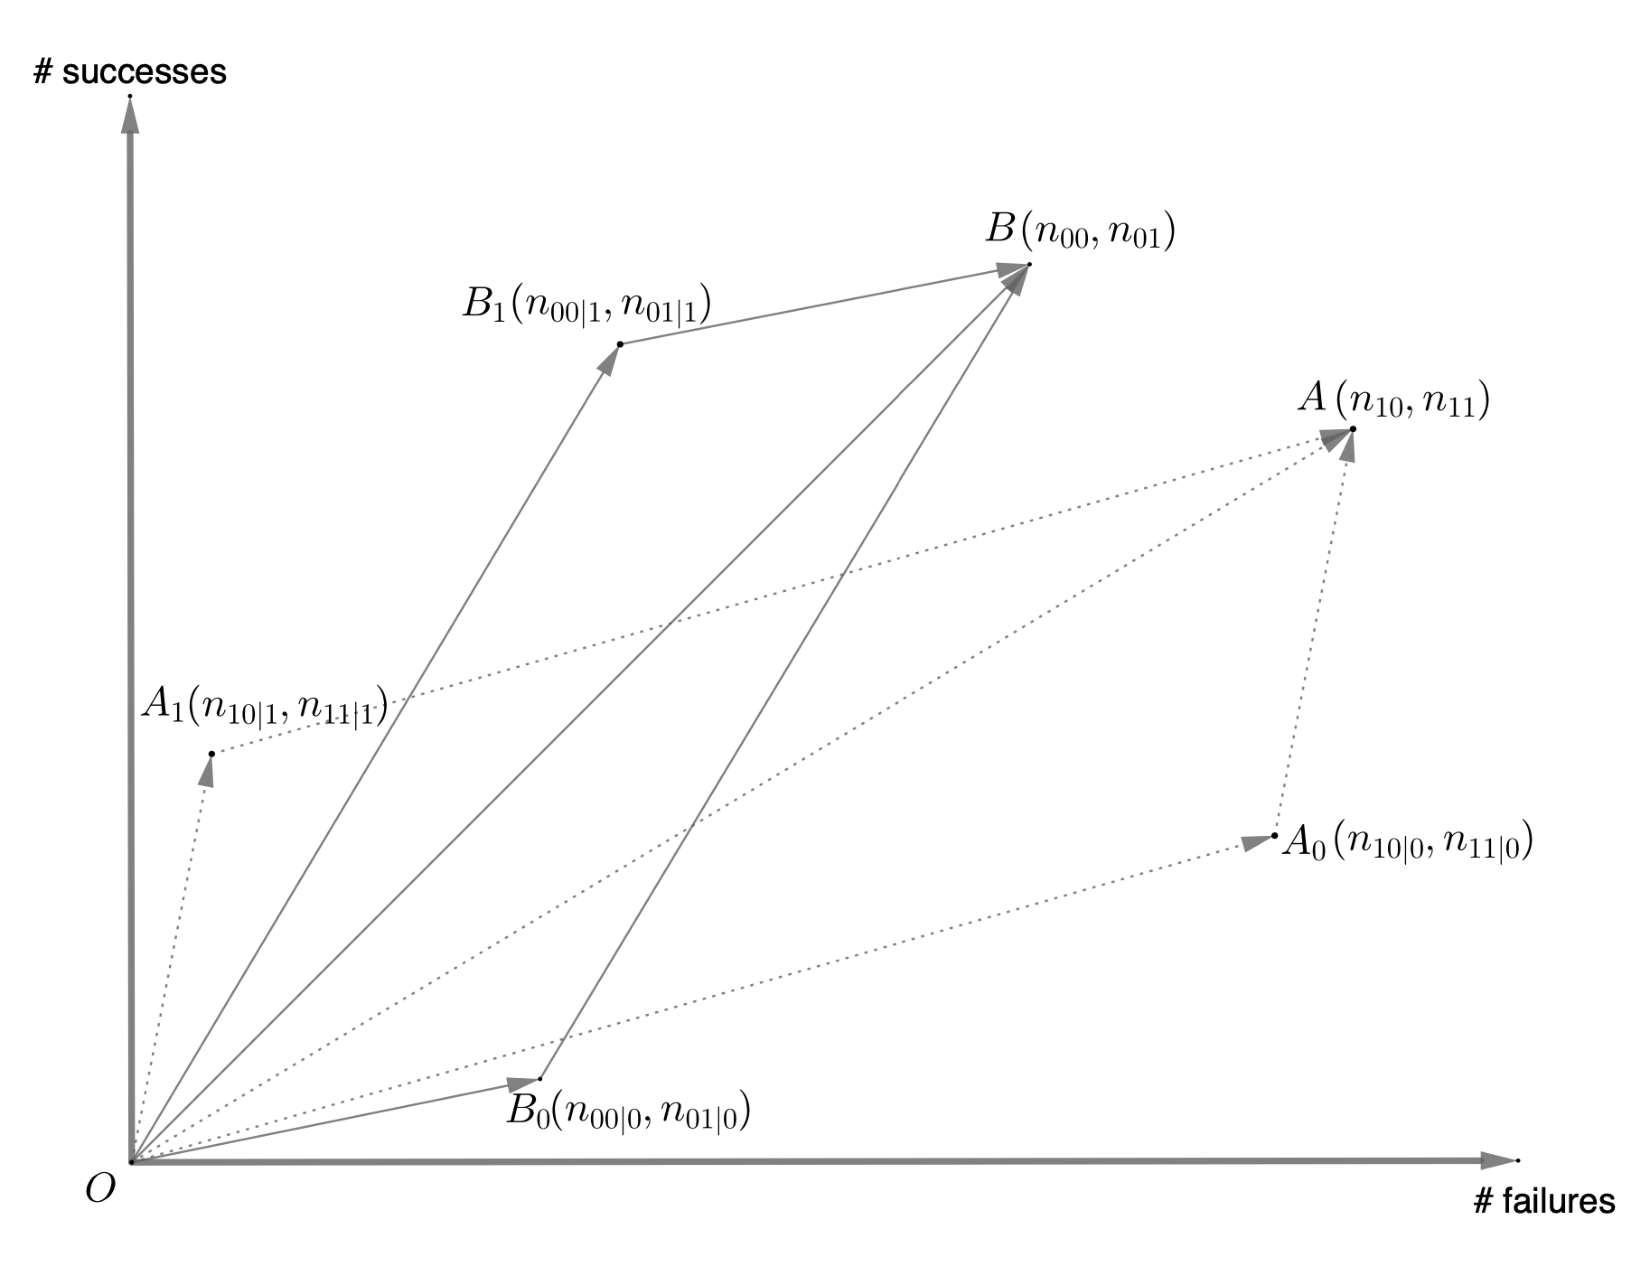
\includegraphics[width=\textwidth]{figures/simpson_geometry2.pdf}
\caption{尤尔-辛普森悖论的几何解释}\label{fig::geomtry-simpson}
\end{figure}

\section{伯克利大学研究生录取数据}
\label{sec::berkeleydata}

\citet{bickel1975sex} 曾研究伯克利大学研究生院的男女录取率差异。\ri{R} 语言的 \ri{datasets} 程序包中包含原始数据集 \ri{UCBAdmissions}。六个最大系别的原始数据如下所示： 
\begin{lstlisting}
> library(datasets)
> UCBAdmissions = aperm(UCBAdmissions, c(2, 1, 3))
> UCBAdmissions
, , Dept = A

        Admit
Gender   Admitted Rejected
  Male        512      313
  Female       89       19

, , Dept = B

        Admit
Gender   Admitted Rejected
  Male        353      207
  Female       17        8

, , Dept = C

        Admit
Gender   Admitted Rejected
  Male        120      205
  Female      202      391

, , Dept = D

        Admit
Gender   Admitted Rejected
  Male        138      279
  Female      131      244

, , Dept = E

        Admit
Gender   Admitted Rejected
  Male         53      138
  Female       94      299

, , Dept = F

        Admit
Gender   Admitted Rejected
  Male         22      351
  Female       24      317
\end{lstlisting}


对全系别数据汇总后可得简洁的二乘二列联表：
\begin{lstlisting} 
> UCBAdmissions.sum = apply(UCBAdmissions, c(1, 2), sum)
> UCBAdmissions.sum
        Admit
Gender   Admitted Rejected
  Male       1198     1493
  Female      557     1278
\end{lstlisting}

下面的函数以\ri{chisq.test}为基础，输入一个二乘二表，输出估计的 \textsc{rd}与$p$值：
\begin{lstlisting}
> risk.difference = function(tb2)
+ {
+   p1      = tb2[1, 1]/(tb2[1, 1] + tb2[1, 2])
+   p2      = tb2[2, 1]/(tb2[2, 1] + tb2[2, 2])
+   testp   = chisq.test(tb2)
+   
+   return(list(p.diff = p1 - p2,  
+               pv = testp$p.value))	    
+ }
\end{lstlisting}
运行该函数可知男女生的录取率存在显著差值：
\begin{lstlisting}
> risk.difference(UCBAdmissions.sum)
$p.diff
[1] 0.1416454

$pv
[1] 1.055797e-21
\end{lstlisting}

若按系别分别分析，则男女生的录取率差异大幅缩小且多不具有统计学显著性。仅在系别 A 中观察到显著的负向差异。 
\begin{lstlisting}
> P.diff = rep(0, 6)
> PV     = rep(0, 6)
> for(dd in 1:6)
+ {
+ 	 department = risk.difference(UCBAdmissions[, , dd])
+ 	 P.diff[dd] = department$p.diff
+ 	 PV[dd]     = department$pv 
+ }
> 
> round(P.diff, 2)
[1] -0.20 -0.05  0.03 -0.02  0.04 -0.01
> round(PV, 2)
[1] 0.00 0.77 0.43 0.64 0.37 0.64
\end{lstlisting} 



 



 
\section{作业习题}


\paragraph{二乘二表格中的独立性}\label{hw::2x2-equivalence}

请证明命题 \ref{prop::2x2-independence} 中的结论 (1) 与 (2)。 


\paragraph{尤尔-辛普森悖论的更多实例}


请构造一个能够产生尤尔-辛普森悖论的三维列联表数值实例。 

请找出现实案例中符合该悖论的实例。 



\paragraph{相关性与偏相关}\label{hw::partial-correlation}

考虑三维正态随机向量
$$
\begin{pmatrix}
X\\
Y\\
Z
\end{pmatrix}
\sim 
\textsc{N}
\left(
\begin{pmatrix}
0\\
0\\
0
\end{pmatrix},
\begin{pmatrix}
1 & \rho_{XY} &\rho_{XZ} \\
  \rho_{XY}  & 1 & \rho_{YZ} \\
  \rho_{XZ} &  \rho_{YZ} & 1
\end{pmatrix}
\right) . 
$$
$Y$与$Z$的相关系数为$\rho_{YZ}$。偏相关系数有多种等价定义。对多元正态向量，用$\rho_{YZ|X}$表示给定$X$后$Y$与$Z$的偏相关系数，即条件分布$(Y, Z)\mid X$中的相关系数。证明
$$
\rho_{YZ\mid X} = \frac{   \rho_{YZ} - \rho_{YX} \rho_{ZX}  }{  \sqrt{  1-\rho_{YX}^2 }  \sqrt{1- \rho_{ZX}^2  }  }  . 
$$

请构造一组满足 $\rho_{YZ} > 0$ 但 $\rho_{YZ|X} < 0$ 的数值实例。 

提示：该实例可视为正态分布下的尤尔-辛普森悖论实例。可借助第 \ref{sec::multivariate-normal} 章的结论推导偏相关系数的表达式。 



\paragraph{变量筛选分析}\label{hw::lalonde-obs-reg}

第\ref{section:correlatioandregressionintro}节重新分析了\citet{hainmueller2012entropy}的数据，结果变量为\ri{re78}，处理为\ri{treat}。数据还含$10$个协变量，所以线性回归有$2^{10} = 1024$个可能的协变量子集。对全部子集拟合$1024$个线性回归，报告处理系数。其中有多少显著为正、多少显著为负、多少不显著？也可报告其他有意思的发现。


\paragraph{种族歧视现象的再探讨}

第 \ref{sec::twobytwotables-withresume} 节重析了 \citet{bertrand2004emily} 收集的数据。请分别针对男性和女性群体独立开展分析，总结各子群的分析结果有何异同？


\paragraph{推荐阅读}

\citet{bickel1975sex}是第\ref{sec::berkeleydata}节悖论的原始文献，\citet{pearl2018book}近期从因果推断视角重新讨论了该研究。 



  \chapter{潜在结果}
 \label{chapter::potential-outcomes}


\section{实验主义者对因果推断的观点}






\citet{rubin1975bayesian}与\citet{holland1986statistics}提出了这样一句格言：
\begin{quote}
“没有干预就没有因果关系。”
\end{quote}
并非所有人都认同这一观点，但它有助于澄清因果思考中的歧义。本书采用这一视角，以潜在结果框架定义因果效应\citep{Neyman:1923, Rubin:1974}。在此框架中，实验或至少思想实验包含一项处理，研究者关心它对一个或多个结果的效应。{\it 处理}有时也称{\it 干预}或{\it 操纵}。 


\begin{example}\label{eg::aspirin}
如果我们想了解服用阿司匹林与否对缓解头痛的效果，那么干预措施就是“服用阿司匹林与否”。 
\end{example}



\begin{example}\label{eg::jobtraining}
如果我们想了解参加职业培训与否对就业率与工资水平的影响，那么干预措施就是“参加职业培训与否”。 
\end{example}


\begin{example}\label{eg::classroom}
如果我们想了解在小班还是大班上课对标准化考试成绩的影响，那么干预措施就是“在小班上课与否”。 
\end{example} 

\begin{example}\label{eg::gotv}
\citet{gerber2008social}研究的是各类鼓励投票的宣传信息对投票行为的影响。此时，干预措施便是这些不同的鼓励投票宣传信息。 
\end{example} 


\begin{example}\label{eg::bmi}
\citet{pearl2018does}指出，我们可以推断肥胖症对寿命的影响。衡量肥胖的常见指标是体质指数（BMI），其定义为身体质量除以身高的平方，单位采用千克/米$^2$。因此，此处的干预措施可以理解为不同水平的BMI值。 
\end{example} 


上述干预的歧义程度不同：例\ref{eg::aspirin}至\ref{eg::gotv}的干预较明确，例\ref{eg::bmi}中干预 BMI 的含义却不够明确。降低 BMI 可以有多种方式，例如改善饮食、增加运动或减重手术，它们对结果的效应可能很不一样。本书认为，若不进一步澄清，例\ref{eg::bmi}中的干预就没有良好定义。

 

另一个定义模糊的干预措施便是“种族”。种族歧视是劳动力市场中的一个重要问题，但要设计试验来改变实验对象的种族却并非易事。\citet{bertrand2004emily}设计了一项有趣的实验，部分回应了这一问题。 

\begin{example}\label{eg::race}
回顾例\ref{eg::bertrand2004emily-chapter1}。\citet{bertrand2004emily}随机改变简历上的姓名，比较带有听起来像非洲裔美国人姓名与白人姓名的简历的回访率。对每份简历，干预是姓名听起来像黑人还是白人的二元指标，结果是是否收到回访的二元指标。第\ref{sec::twobytwotables-withresume}节分析了如下二乘二表： 

\begin{center} 
\begin{tabular}{ccc}
\hline 
 &   获得回电 & 未获得回电 \\
 \hline 
非洲裔美国人风格姓氏  & 157 & 2278\\
欧洲裔美国人风格姓氏   & 235 & 2200\\
\hline 
\end{tabular}
\end{center}

根据此表，我们可以计算两种姓氏获得回电的概率之差：
$$
\frac{157}{2278 + 157} - \frac{235}{  2200 + 235 } = 6.45\% - 9.65\% = - 3.20\% < 0
$$
费舍尔精确检验得到的$p$值也显著小于$0.001$。 
\end{example}

在\citet{bertrand2004emily}的实验中，处理是实验者能够操纵的{\it 被感知的种族}，从而回答一个定义明确的因果问题。但批评者可能指出，对被感知种族的干预，其因果效应未必等于实际种族的因果效应。 



\section{潜在结果的正式记号}
\label{sec::po-sciencetable}

考虑一项有$n$个实验单位的研究，编号为$i= 1, \ldots, n$。先讨论二水平处理：$1$表示处理，$0$表示对照。每个单位$i$的目标结果$Y$有两个版本：
$$
Y_i(1)  \text{ and } Y_i(0),
$$
即假想干预 1 和 0 下的潜在结果。 
%The founding father of the Statistics Department at the University of California Berkeley, Professor Jerzy Neyman, first used this notation in his thesis written in Polish \citep{Neyman:1923}. 
\citet{Neyman:1923}首次使用了这一记号。它看似直观，却隐含一些假设，\citet{Rubin:1980}对此作了如下澄清。

\begin{assumption}
[无相互干扰]
\label{sutva1}
单位$i$的潜在结果不依赖其他单位接受的处理，有时称为{\it 无干扰}假设。 
\end{assumption}


\begin{assumption}
[一致性]
\label{sutva2}
处理不存在未区分的其他版本。等价地，要求处理水平定义明确，至少对所关心的结果没有歧义。这有时称为{\it 一致性}假设。\footnote{这种一致性与第\ref{chapter::basic-prob-append}章定义\ref{def::consistency}中估计量的一致性完全不同。} 
\end{assumption}


%\begin{enumerate}
%[(1)]
%\item\label{sutva1}
%Unit $i$'s potential outcomes do not depend on other units' treatments. This is sometimes called the {\it no-interference} assumption. 
%
%\item\label{sutva2}
%There are no other versions of the treatment. Equivalently, we require that the treatment level be well-defined, or have no ambiguity at least for the outcome of interest. This is sometimes called the {\it consistency} assumption. 
%
%\end{enumerate}

上述假设\ref{sutva1}在传染病研究或网络实验中可能被违反。例如，如果我的某些朋友接种了流感疫苗，即便我没有接种，我患流感的可能性也会降低；如果我的朋友们看到了脸书上的广告，即便我没看到该广告，我购买相应产品的可能性也会提高。在现代因果推断文献中，研究存在相互干扰的实验对象这一情形属于一个活跃的研究领域\citep[e.g.,][]{hudgens2008toward}。 


假设\ref{sutva2}则可能在涉及多种成分的复杂干预措施下被违反。例如，在研究吸烟对肺癌的影响时，香烟的种类可能是个重要因素；在考察高等教育对收入的影响时，大学教育的类型与专业也可能发挥关键作用。 


\citet{Rubin:1980}将上述假设\ref{sutva1}与\ref{sutva2}合称为“稳定单元处理值假设”（Stable Unit Treatment Value Assumption，简称SUTVA）。


\begin{assumption}
[SUTVA]
\label{sutva-complete}
假设\ref{sutva1}与\ref{sutva2}均成立。
\end{assumption}


在SUTVA成立的前提下，\citet{Rubin:2005}将包含所有潜在结果的$n\times 2$矩阵称为“科学表格”：
\begin{center}
\begin{tabular}{ccc}
\hline 
$i$ & $Y_i(1)$ &  $Y_i(0)$ \\
 \hline 
$1$ & $Y_1(1)$ &  $Y_1(0)$ \\
$2$ & $Y_2(1)$ &  $Y_2(0)$ \\
\vdots  &\vdots & \vdots   \\
$n$ & $Y_n(1)$ &  $Y_n(0)$ \\
\hline 
\end{tabular}
\end{center}  


由于Neyman与Rubin对统计因果推断做出了奠基性贡献，潜在结果框架有时也被称作“Neyman模型”“Neyman-Rubin模型”或“Rubin因果模型”。不过在本书及其他科学著作中，我更倾向于使用“潜在结果框架”这一称呼。 
 
 
因果效应是科学表的函数。推断个体因果效应
$$
\tau_i =  Y_i(1) - Y_i(0) ,\quad (i=1, \ldots, n)
$$
存在根本困难：对每个单位$i$，只能观测$Y_i(1)$或$Y_i(0)$之一，也就是科学表的一半。作为起点，本书多数部分关注平均因果效应（ACE）：
\begin{eqnarray*}
\tau  &=&  n^{-1} \sumn \{  Y_i(1) - Y_i(0) \}  \\
&=&  n^{-1} \sumn  Y_i(1) -  n^{-1} \sumn  Y_i(0).
\end{eqnarray*}
也可推广到许多其他参数，亦称{\it 估计目标}，例子见习题\ref{hw::nonlinear-causal-estimands}。 


\subsection{因果效应、子组以及尤尔-辛普森悖论的不可能性}


若由二元变量$X_i $定义两个亚组，可定义亚组因果效应
$$
\tau_x = \frac{  \sumn  I(X_i = x) \{  Y_i(1) - Y_i(0) \}    }{   \sumn  I(X_i = x)    },\quad (x=0,1) 
$$
其中$I(\cdot)$为指示函数。有简单恒等式
$$
\tau =  \pi_1 \tau_1  +  \pi_0 \tau_0
$$
其中$\pi_x =  \sumn  I(X_i = x)  / n$是满足$X_i = x$的单位比例，$(x=0,1)$。因此，若$\tau_1  > 0$且$ \tau_0 > 0$，必有$\tau > 0$。所以 Yule--Simpson 悖论不会发生在这种因果效应的汇总中。  



\subsection{实验单位定义中的细微之处}

实验单位的定义有一个微妙之处：实验单位未必等同于物理对象。例如，我之前未服阿司匹林，头痛没有消失；现在服药，头痛消失。你可能以为观察到了我在对照和处理下的两个潜在结果。用$i$表示我，令$Y=1$表示无头痛，似乎$Y_i(0) = 0$、$Y_i(1) = 1$，所以阿司匹林治好了头痛。但这一逻辑误解了实验单位。同一个人在不同时间点，是两个不同的实验单位，编号为“$i,\textup{before}$”与“$i,\textup{after}$”。因此共有四个潜在结果
$$
Y_{i,\textup{before}}(0)=0, \quad  Y_{i,\textup{before}}(1)=?,\quad
Y_{i,\textup{after}}(0)=?, \quad  Y_{i,\textup{after}}(1)=1,
$$
其中两个已观测，两个缺失，个体因果效应
$$
Y_{i,\textup{before}}(1) -  Y_{i,\textup{before}}(0) = ? - 0 \text{ and } Y_{i,\textup{after}}(1)  - Y_{i,\textup{after}}(0) = 1 - ?
$$
仍未知。即使不服药，头痛也可能自行消失：
$$
Y_{i,\textup{after}}(0)=1, \quad  Y_{i,\textup{after}}(1)=1
$$
此时效应为零；也可能不服药就不会消失：
$$
Y_{i,\textup{after}}(0)=0, \quad  Y_{i,\textup{after}}(1)=1
$$
此时阿司匹林效应为正。 

若前后两期的对照潜在结果稳定，
$$
Y_{i,\textup{before}}(0) = Y_{i,\textup{after}}(0) = 0 .
$$
上述错误的直观推理也可能碰巧得到正确答案。但这是很强且根本不可检验的假设。\citet{rubin2001comment}在因果效应的自我实验背景下作了相关讨论。



\section{干预措施分配机制}\label{sec::Treatment-ScienceTable}

令$Z_i$为单位$i$的二元处理指标，组成向量$\bm{Z} = (Z_1, \ldots, Z_n)$。单位$i$的观测结果是潜在结果与处理指标的函数：
\begin{eqnarray} 
Y_i &=& \begin{cases}
   Y_i(1),& \text{if } Z_i = 1\\
   Y_i(0), & \text{if } Z_i = 0
\end{cases} \label{eq::yobsdef} \\
&=& Z_i Y_i(1) + (1-Z_i)Y_i(0) \label{eq::fundamentalbridge} \\
&=& Y_i(0)  + Z_i\{  Y_i(1) - Y_i(0)  \} \label{eq::teh} \\
&=&Y_i(0)  + Z_i\tau_i . \label{eq::teh2} 
\end{eqnarray}
\eqref{eq::yobsdef}定义观测结果，\eqref{eq::fundamentalbridge}与\eqref{eq::yobsdef}等价。虽然这是简单事实，\citet{pearl2010brief}将其视为连接潜在结果与观测结果的基本桥梁。公式\eqref{eq::teh}与\eqref{eq::teh2}表明，个体因果效应$\tau_i =  Y_i(1) - Y_i(0)  $可因单位而异。 


实验只揭示单位$i$的一个潜在结果，另一个缺失：
\begin{eqnarray*} 
Y_i^\textup{mis} &=& \begin{cases}
   Y_i(0),& \text{if } Z_i = 1\\
   Y_i(1), & \text{if } Z_i = 0
\end{cases}  \\
&=& Z_i Y_i(0) + (1-Z_i)Y_i(1) .
\end{eqnarray*}
缺失结果对应单位$i$没有接受的那个处理水平，因此潜在结果框架也称{\it 反事实}框架。\footnote{“反事实”在哲学中更常见，可能与\citet{lewis1973causation}有关。}这个名称可能引起误解：实验前，两个潜在结果都有可能被观测；实验后，一个成为观测结果，另一个才是反事实结果。 


干预措施分配机制——即向量$\bm{Z} $的概率分布——对推断因果效应起着重要作用。以下简单数值示例可阐明这一点。我们先从正态分布中生成潜在结果，并使平均因果效应接近$-0.5$。 
\begin{lstlisting}
> n  = 500
> Y0 = rnorm(n)
> tau = - 0.5 + Y0
> Y1 = Y0 + tau
\end{lstlisting} 
优秀的医生会在知晓某位患者个体因果效应非负时才安排其接受干预。如此一来，观测结果的均值差将呈现正值： 
\begin{lstlisting}
> Z = (tau >= 0)
> Y = Z*Y1 + (1 - Z)*Y0
> mean(Y[Z==1]) - mean(Y[Z==0])
[1] 2.166509
\end{lstlisting} 
%Another perfect doctor ranks the individual causal effects and assigns the treatment to the patient if the rank is larger than or equal to $n/2$. This again results in a positive difference in means of the observed outcomes: 
%\begin{lstlisting}
%> Z = (rank(tau) >= n/2)
%> Y = Z*Y1 + (1 - Z)*Y0
%> mean(Y[Z==1]) - mean(Y[Z==0])
%[1] 1.851417
% \end{lstlisting} 
而毫无经验可言的医生因不了解任何个体因果效应信息，只能随机安排干预措施。此时观测结果的均值差则会接近真实的平均因果效应值： 
\begin{lstlisting}
> Z = rbinom(n, 1, 0.5)
> Y = Z*Y1 + (1 - Z)*Y0
> mean(Y[Z==1]) - mean(Y[Z==0])
[1] -0.552064 
  \end{lstlisting} 
  
 以上例子虽属假设，现实中没有医生能完全知晓个体因果效应值。这些例子仍足以说明干预措施分配机制的关键作用。本书后续内容也将围绕该机制展开论述。 




 
\section{作业习题}



\paragraph{优秀的医生}
\label{hw::perfect-doctor}

参照第\ref{sec::Treatment-ScienceTable}节中那位优秀医生的例子，假设潜在结果由如下方式生成：
$$
Y(0) \sim \textsc{N}(0,1), \quad \tau = -0.5 + Y(0),\quad Y(1)  = Y(0) + \tau .
$$
干预措施则由因果效应值决定：$Z = 1(\tau \geq 0)$，观测结果亦随之确定为$Y = ZY(1) + (1-Z) Y(0)$。现请计算两种干预水平下观测结果的均值差：
$$
E(Y\mid Z=1) - E(Y\mid Z=0).
$$


提示：截断正态随机变量的均值计算公式如下：
$$
E(X\mid   a < X < b ) = \mu - \sigma \frac{   \phi \left(  \frac{b-\mu}{\sigma} \right )   -  \phi \left(  \frac{a-\mu}{\sigma} \right )   }
{   \Phi \left(  \frac{b-\mu}{\sigma} \right )   -  \Phi \left(  \frac{a-\mu}{\sigma} \right )   } , 
$$
其中$X \sim \textsc{N}(\mu, \sigma^2)$，$\phi(\cdot)$与$\Phi(\cdot)$分别为标准正态随机变量$\textsc{N}(0,1)$的概率密度函数与累积分布函数。 



\paragraph{非线性因果估计量}
\label{hw::nonlinear-causal-estimands}



有$n$个单位的处理与对照潜在结果$\{  (Y_i(1), Y_i(0) \}_{i=1}^n$时，均值差等于个体处理效应的均值：
$$
\bar{Y}(1) - \bar{Y}(0) = n^{-1} \sum_{i=1}^n  \{ Y_i(1) - Y_i(0) \}.
$$
因此，平均处理效应是{\it 线性}因果估计目标：潜在结果均值之差等于个体潜在结果之差的均值。 


其他估计目标未必线性。例如，可定义中位数处理效应
$$
\delta_1 = \text{median}\{  (Y_i(1) \}_{i=1}^n - \text{median}\{  (Y_i(0) \}_{i=1}^n,
$$
它一般不同于个体处理效应的中位数
$$
\delta_2 = \text{median}\{  (Y_i(1) - Y_i(0) \}_{i=1}^n .
$$

\begin{enumerate}
\item
请分别给出数值实例使上述两种估计量满足$\delta_1 = \delta_2$、$\delta_1 > \delta_2$与$\delta_1 < \delta_2$的情形。 


\item
$\delta_1$与$\delta_2$哪个更有意义？为什么？用例子说明。若认为$\delta_1$与$\delta_2$在不同应用中都可能合理，也可分别举例论证。 
\end{enumerate}




\paragraph{平均效应与个体效应}

给出数值例子，使$\tau = n^{-1} \sum_{i=1}^n  \{ Y_i(1) - Y_i(0) \}  >0$成立，但满足$Y_i(1) > Y_i(0)$的单位比例小于$0.5$。即平均因果效应为正，处理却使不到一半的单位获益。 


\paragraph{推荐阅读}

\citet{holland1986statistics}是统计因果推断的经典综述，使潜在结果框架的“Rubin 因果模型”这一名称广为人知。在加州大学伯克利分校，出于显而易见的原因，我们称之为“Neyman 模型”。  



 
\part{随机实验}\label{part::rcts}
  
\chapter{完全随机化实验与费舍尔随机化检验}\label{ch::frt-cre}
 \chaptermark{完全随机化实验与FRT}


潜在结果框架与随机化实验之间存在着内在联系。理解各类随机化实验中的因果推断机制至关重要，这也有助于我们理解更为复杂的非实验性研究中的因果推断问题。  


本书的\ref{part::rcts}部分主要探讨随机化实验。本章则着重介绍最为简单的实验形式，即完全随机化实验（CRE）。 

\section{CRE}

考虑一个实验，共有$n$个单位参与，其中$n_1$个单位接受处理，$n_0$个单位作为对照。我们可以根据处理分配机制来定义平均因果效应\footnote{。读者可能会认为，在平均因果效应中，$Z_i$相当于独立同分布且服从伯努利分布的随机变量，其概率为$\pi$；此时$n_1$则是一个服从二项分布的$(n,\pi)$随机变量。这种实验形式被称为伯努利随机化实验；若以$(n_1, n_0)$作为条件，该实验便等同于平均因果效应实验。  
我会在第\ref{chapter::neyman-cr}章的习题\ref{hw::bre-inference}中进一步详述伯努利随机化实验的相关内容。  
}

\begin{definition}
[CRE]\label{def::CRE}
固定 $n_1$ 与 $n_0$，并使 $n = n_1 + n_0$。  
一个具有可忽略性条件的随机化实验的处理分配机制为：  
$$
\pr(  \bm{Z} = \bm{z} ) = 1 \Big / \binom{n}{n_1},
$$  
其中 $\bm{z} = (z_1,\ldots, z_n)$ 需满足 $\sumn z_i  = n_1$ 与 $\sumn (1-z_i)  = n_0 . $。
\end{definition}


在定义 \ref{def::CRE} 中，我们假设处理状态下的潜在结果向量 $\bm{Y}(1) = (Y_1(1), \ldots, Y_n(1) )$ 与对照状态下的潜在结果向量 $\bm{Y}(0) = (Y_1(0), \ldots, Y_n(0) )$ 均为固定值。即便我们将它们视为随机变量，也可以以它们为条件，此时处理分配机制便变为
$$
\pr\{    \bm{Z} = \bm{z} \mid \bm{Y}(1), \bm{Y}(0)  \} = 1 \Big / \binom{n}{n_1} 
$$
这是因为在 CRE 条件下满足 $ \bm{Z} \ind \{\bm{Y}(1), \bm{Y}(0)\}$。在 CRE 中，处理向量 $\bm{Z}$ 是由 $n_1$ 个 1 和 $n_0$ 个 0 随机排列所得。

在其具有开创性意义的著作{\it《实验设计》}中，\citet{Fisher:1935}指出了随机化的以下几项优势：
\begin{enumerate}
[(1)]
\item\label{eq::comparable}
这样平均而言便能形成可比较的处理组与对照组。

\item\label{eq::reasonedbasis}
它构成了统计推断的“合理依据”。 
 \end{enumerate}
 
 
点\ref{eq::comparable}的含义较为直观，因为随机化处理并不会使结果偏向处理组或对照组。大多数人都能很好地理解这一点。而点\ref{eq::reasonedbasis}则更为微妙。费舍尔想要表达的意思是：随机化过程能够为统计检验提供依据，这种检验如今被称为费舍尔随机化检验（FRT）。本章将在条件随机化假设下阐述FRT的基本思想。


\section{FRT}
\label{sec::frt-basics}

\citet{Fisher:1935} 有兴趣检验下述零假设：\footnote{ 实际上，\citet{Fisher:1935} 并未使用这种形式的$\HF$，因为他并未采用“潜在结果”这一记号。这种形式是由\citet{Rubin:1980}提出的。}
$$
\HF: Y_i(1) = Y_i(0) \text{ for all units } i=1,\ldots, n.
$$
\citet{Rubin:1980} 将其称为{\it 尖锐零假设}，其含义是：该假设能够基于观测数据确定所有潜在结果，即$\bm{Y}(1) = \bm{Y}(0) =  \bm{Y} = (Y_1, \ldots, Y_n)$——也就是观测结果的向量。它也被称作{\it 强零假设} \citep[e.g.,][]{wu2018randomization}。 


从概念上讲，在$\HF$条件下，FRT方法适用于任何由观测数据所构成的检验统计量\begin{eqnarray}\label{eq::teststatistic}
T = T( \bm{Z}, \bm{Y})  ,
\end{eqnarray}在$\HF$条件下，观测到的结果向量$\bm{Y}$是固定不变的，因此检验统计量$T$中唯一的随机成分便是处理向量$\bm{Z}$。实验者可以自行设定$\bm{Z}$的分布情况，而该分布又决定了$T$在$\HF$条件下的分布。这正是计算$p$值的基础。下文我将作更详细的说明。 


在随机化实验中，$\bm{Z}$在如下集合上呈均匀分布：
$$
\{  \bm{z}^1, \ldots, \bm{z}^M  \}
$$
其中$M = \binom{n}{n_1}$，而各个$ \bm{z}^m$则是所有由$n_1$个$1$和$n_0$个$0$所组成的可能向量。
例如，当$n=5$且$n_1=3$时，我们可以列举出$M = \binom{5}{3} = 10$个向量，具体如下：
\begin{lstlisting}
> permutation10 = function(n, n1){
+  M  = choose(n, n1)
+  treat.index = combn(n, n1)
+  Z = matrix(0, n, M)
+  for(m in 1:M){
+    treat  = treat.index[, m]
+    Z[treat, m] = 1
+  }
+  Z
+ }
> 
> permutation10(5, 3)
     [,1] [,2] [,3] [,4] [,5] [,6] [,7] [,8] [,9] [,10]
[1,]    1    1    1    1    1    1    0    0    0     0
[2,]    1    1    1    0    0    0    1    1    1     0
[3,]    1    0    0    1    1    0    1    1    0     1
[4,]    0    1    0    1    0    1    1    0    1     1
[5,]    0    0    1    0    1    1    0    1    1     1
\end{lstlisting}

因此，$T$ 在该集合上呈均匀分布（集合中可能存在重复元素）
$$
\{   T(\bm{z}^1,\bm{Y}) , \ldots, T( \bm{z}^M, \bm{Y})  \}.
$$
也就是说，由于CRE的设计，我们能够知晓$T$的分布情况。我们将这种$T$的分布称为{\it 随机化分布}。 




如果对于$T$而言数值越大表示越极端，那么我们可以利用以下的尾部概率来衡量该检验统计量相对于其随机化分布的极端程度：\footnote{正因如此，\eqref{eq::exactpvalue}中的$p_\frt$属于单侧概率。有时我们可能希望定义双侧$p$值。一种可行的方法是：若$T$的分布以$0$为中心，则可取其绝对值来计算。}

\begin{equation}\label{eq::exactpvalue}
p_\frt = M^{-1} \sum_{m=1}^M   I\{ T(\bm{z}^m,\bm{Y})   \geq T(\bm{Z},\bm{Y})   \},
\end{equation}

费舍尔将此类值称为$p$值。图\ref{fig::frt}展示了$p_\frt $的计算过程。 



\begin{figure}[ht]
\centering 
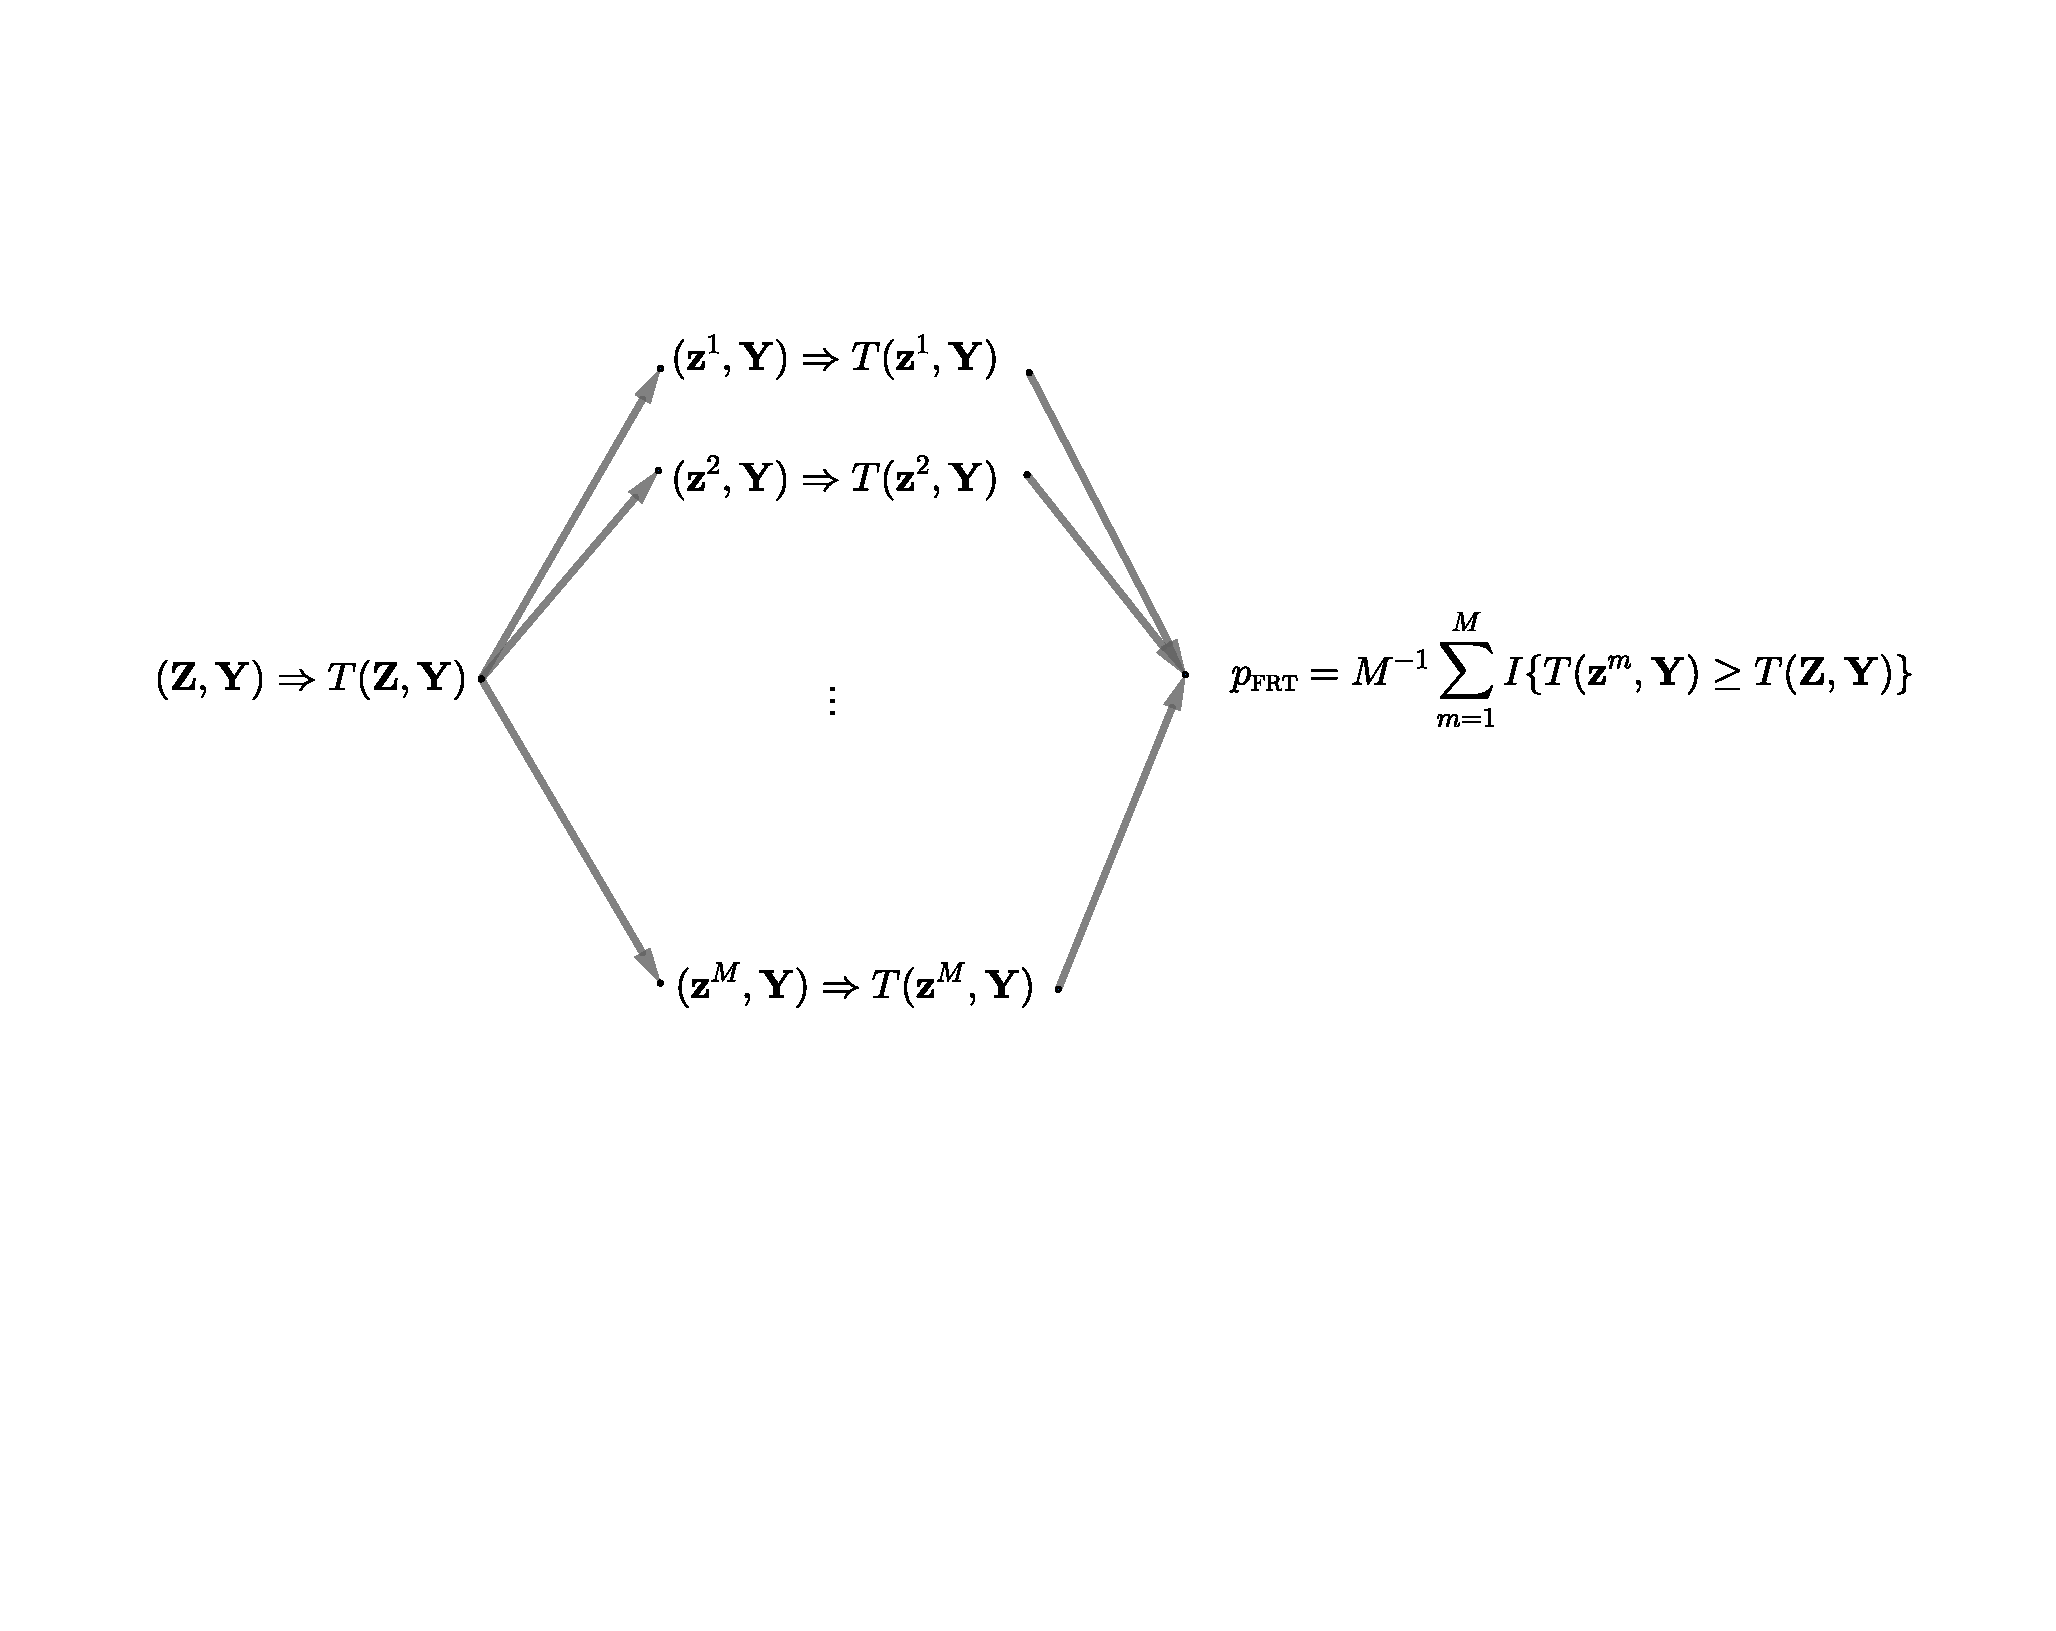
\includegraphics[width =  \textwidth]{figures/frt_fig.pdf}
\caption{ FRT示意图}\label{fig::frt}
\end{figure}




$p$值，即$p_\frt$，在\eqref{eq::exactpvalue}中对任意检验统计量的选择以及任意结果生成过程均适用。该结论还能自然地推广至任意实验情形，这也是后续章节中将反复探讨的主题。重要的是，从\footnote{的意义上来说，该值具有有限样本下的精确性。这正是数理统计学中对$p$值的标准定义。出现不等式的原因通常在于检验统计量的离散性；而当等式成立时，在零假设下$p$值服从$(0,1)$上的均匀分布。设$F(\cdot)$为$T(\bm{Z},\bm{Y})$的分布函数。尽管该分布函数属于阶梯函数，我们仍假定其连续且严格单调递增，就如同它是定义在整个实数轴上的某个连续随机变量的分布函数一般。因此$p_\frt = 1- F(T)$，并且
$$
\pr(p_\frt \leq u) = \pr\{ 1-F(T) \leq u\} = \pr\{  T \geq F^{-1}(1-u)  \} = 1- F( F^{-1}(1-u)) = u.
$$
$T$的离散性确实会在证明过程中引发一些技术性问题，从而导致出现不等式而非等式。具体的技术细节则留作习题\ref{hw::exact-frt}加以探讨。}即在$\HF$条件下，
\begin{eqnarray}\label{eq::p-value-valid}
\pr(p_\frt \leq u) \leq u \quad  \text{ for all } \quad 0 \leq u \leq 1.
\end{eqnarray}




在实践中，$M$的值通常过大（例如，当$n=100, n_1=50$时，我们有$M > 10^{29}$），因此要枚举出处理向量所有可能的取值在计算上是不可行的。我们通常借助蒙特卡洛方法来近似计算$p_\frt$（关于蒙特卡洛方法的基本介绍可参见\ref{sec::monte-carlo-method}节）。具体而言，我们从处理向量的所有可能取值中独立抽取随机样本；或者等价地说，我们对$\bm{Z}$进行随机排列，随后利用下式来近似$p_\frt$：
\begin{equation}\label{eq::mcpvalue}
\hat p_\frt  =  R^{-1} \sum_{r=1}^R   I\{ T(\bm{z}^r,\bm{Y})   \geq T(\bm{Z},\bm{Y})   \},
\end{equation}
其中$\bm{z}^r$代表$R$次对$\bm{Z}$的随机排列。

在\eqref{eq::mcpvalue}中，随着$R$值的增大，$p$值对应的蒙特卡洛误差会迅速减小；详见\ref{para::monte-carlo-error-pfrt}题。由于计算\eqref{eq::mcpvalue}中的$p$值需要用到$\bm{Z}$的排列运算，因此在CRE背景下，FRT有时也被称作{\it 排列检验}。不过，FRT的理念其实比那些用于较复杂实验的排列检验更为通用。 



\section{检验统计量的典型选择}
\label{sec::frt-choiceofstatistic}

根据上述讨论可知，无论选择何种检验统计量，FRT都能产生有限样本下的精确$p$值。这正是FRT的一个特性。不过，这一特性并不应成为随意选择检验统计量的依据。直观而言，我们应当选择那些能够反映$\HF$是否可能被违反的检验统计量。下文我将介绍一些典型的检验统计量选择方式。 


\begin{example}[均值差法]\label{eq::frt-difference-in-means}
均值差统计量即为
$$
\hat{\tau}   = \hat{\bar{Y}}(1) - \hat{\bar{Y}}(0)
$$
其中
$$
 \hat{\bar{Y}}(1)  =  n_1^{-1} \sum_{Z_i=1} Y_i  = n_1^{-1} \sumn Z_iY_i 
$$
表示接受处理时观测结果的样本均值，而
$$
\hat{\bar{Y}}(0) = n_0^{-1}  \sum_{Z_i=0} Y_i   = n_0^{-1}  \sumn (1-Z_i) Y_i 
$$
表示对照组中观测结果的样本均值。
%
%\begin{eqnarray*}
%\hat{\tau}  &=& n_1^{-1} \sum_{Z_i=1} Y_i - n_0^{-1}  \sum_{Z_i=0} Y_i  \\
%&=&  n_1^{-1} \sumn Z_iY_i - n_0^{-1}  \sumn (1-Z_i) Y_i  \\
%&\equiv & \hat{\bar{Y}}(1) - \hat{\bar{Y}}(0).
%\end{eqnarray*}
在$\HF$条件下，其均值为
$$
E(  \hat{\tau}    ) = n_1^{-1}\sumn E(Z_i)Y_i  - n_0^{-1}  \sumn E(1-Z_i) Y_i  = 0
$$
方差则为
\begin{eqnarray*}
\var( \hat{\tau}   ) &=& \var\left\{  n_1^{-1} \sumn Z_iY_i - n_0^{-1}  \sumn (1-Z_i) Y_i  \right\} \\
&=&\var\left(  \frac{n}{n_0}    \frac{1}{n_1} \sumn  Z_i Y_i         \right) \\
&=_*& \frac{n^2}{n_0^2} \left( 1 - \frac{n_1}{n} \right) \frac{s^2}{n_1} \\ 
&=& \frac{n}{n_1 n_0} s^2,
\end{eqnarray*}
其中$=_*$这一结论是根据针对简单随机抽样的\ref{lemma::samplemean}号引理以及$$
\bar{Y} = n^{-1}  \sumn Y_i,\quad 
s^2 = (n-1)^{-1} \sumn (Y_i - \bar{Y})^2 .  
$$得出的。
此外，根据\ref{lemma::finite-population-clt}号引理中所述的有限总体中心极限定理，$\hat{\tau}$的随机化分布近似呈正态分布：
\begin{equation}\label{eq::frt-tau-hat}
\frac{  \hat{\tau}      }{  \sqrt{\frac{n}{n_1 n_0} s^2}    }  
%= \frac{  n_1^{-1} \sum_{Z_i=1} Y_i - n_0^{-1}  \sum_{Z_i=0} Y_i  }{ \sqrt{   \frac{n}{n_1 n_0(n-1)}    \sumn (Y_i - \bar{Y})^2   }  }   
\rightarrow  \N01 
\end{equation}
其分布符合该规律。由于$s^2$在$\HF$条件下为固定值，因此在FRT中将其替换为$$
\frac{  \hat{\tau}      }{  \sqrt{\frac{n}{n_1 n_0} s^2}    }  
$$作为检验统计量同样可行；正如\eqref{eq::frt-tau-hat}所示，该统计量渐进地服从$\textsc{N}(0,1)$分布。如此我们便可计算出近似的$p$值。 
\end{example}


观测到的数据为 $\{  Y_i: Z_i = 1 \}$ 与 $\{ Y_i : Z_i = 0 \}$，因此该问题本质上属于双样本问题。  
在假定结果变量服从独立同分布的正态分布这一前提下（参见第 \ref{sec::bf-problem} 节），经典的、假设方差相等的双样本 $t$ 检验是基于如下公式：
\begin{equation}\label{eq::two-sample-t-equalv}
\frac{  \hat{\tau}      }{  \sqrt{\frac{n}{n_1 n_0(n-2)}  \left[  \sum_{Z_i=1}  \{Y_i - \hat{\bar{Y}}(1)\}^2
+ \sum_{Z_i=0}  \{Y_i - \hat{\bar{Y}}(0)\}^2
    \right]  }    }   \sim t_{n-2}.
\end{equation}
通过一些代数运算（参见习题 \ref{hw::frt-algebraic-detail}），可得到如下展开式：
\begin{equation}\label{eq::frt-algebra-difference-in-means}
(n-1)s^2 = \sum_{Z_i=1}  \{Y_i - \hat{\bar{Y}}(1)\}^2 + \sum_{Z_i=0}  \{Y_i - \hat{\bar{Y}}(0)\}^2
+ \frac{n_1 n_0}{n} \hat{\tau}^2 .
\end{equation}
当样本量 $n$ 较大时，我们可以忽略 $\N01$ 与 $t_{n-2}$ 之间的差异，以及 $n-1$ 与 $n-2$ 之间的差异。  
此外，在 $\HF,$ 条件下，$\hat{\tau}$ 依概率收敛至零，因此从渐近角度而言 $ n_1 n_0 / n \hat{\tau}^2$ 可忽略不计。于是，在 $\HF,$ 条件下，例 \ref{eq::frt-difference-in-means} 中计算出的近似 $p$ 值会接近于经典等方差双样本 $t$ 检验所算出的 $p$ 值；后者可通过 \ri{t.test} 结合 \ri{var.equal = TRUE} 来计算得出。而在 $\tau$ 不为零的备择假设下，展开式 \eqref{eq::frt-algebra-difference-in-means} 中的附加项 $\frac{n_1 n_0}{n} \hat{\tau}^2$ 可能导致 FRT 的功效低于常规的 $t$ 检验；\citet{Ding:2014} 曾指出这一点。 


基于上述讨论，采用$\hat{\tau}$的FRT实际上是利用了合并方差，而忽略了两组之间的异方差性。在经典统计学中，具有异方差性正态分布结果的双样本问题被称为贝伦斯-费舍尔问题（详见\ref{sec::bf-problem}节）。在该问题中，最常用的检验统计量即为下述的学生化统计量。 



\begin{example}[学生化统计量]
\label{eg::studentized-statistic}
该学生化统计量\footnote{此处使用$t$这一符号是有意为之，因为它与$t$分布相关。不过不应将其与符号$t_\nu$相混淆，后者表示自由度为$\nu$的$t$分布。}的计算公式为
$$
t = \frac{    \hat{\bar{Y}}(1)  -   \hat{\bar{Y}}(0)    }{  \sqrt{  \frac{  \hat{S}^2(1)  }{n_1}  + \frac{\hat{S}^2(0)}{n_0}  }   },
$$
其中
$$
\hat{S}^2(1) = (n_1 - 1)^{-1} \sum_{Z_i =1} \{ Y_i  -\hat{\bar{Y}}(1)   \}^2,\quad
\hat{S}^2(0) = (n_0 - 1)^{-1} \sum_{Z_i =0} \{ Y_i  -\hat{\bar{Y}}(0)   \}^2 
$$
分别代表处理组与对照组中观测结果的样本方差。在$\HF$条件下，有限总体中心极限定理再次表明：$t$呈渐近正态分布：
$$
t \rightarrow \N01 
$$
即服从该分布。
随后我们便可计算出一个近似的$p$值，该值接近于由\ri{t.test}及\ri{var.equal = FALSE}所得出的$p$值。
\end{example}



一个极其重要的观点是：即便基础分布并非正态分布，FRT方法也能为那些使用\ri{t.test}并结合\ri{var.equal = TRUE}或\ri{var.equal = FALSE}的传统$t$检验提供合理性依据。通常的统计学教材均基于正态分布这一假设来阐述$t$检验的合理性，但该假设在现实应用中可能过于严苛。幸运的是，只要有限总体中心极限定理成立，我们依然可以运用$t$检验程序。即便我们不认同这些中心极限定理，仍可借助$\hat{\tau}$与$t$作为FRT中的检验统计量，从而获得有限样本下的精确$p$值。 


我们将在第\ref{chapter::unification-fisher-neyman}章从另一个角度来阐述这一学生化统计量的合理性。该章节的理论表明，在FRT中使用$t$能够增强对两组间异方差性的稳健性。 


下述检验统计量对于由重尾分布的结果数据所产生的异常值具有稳健性。 




\begin{example}[威尔科克森秩和]\label{example::wilcoxon-cre}
均值差统计量$ \hat{\tau} $利用原始结果的样本均值进行计算，其抽样分布取决于结果的方差。而学生化统计量$t$则利用原始结果的样本均值与方差进行计算，其抽样分布取决于结果的更高阶矩。正因如此，$ \hat{\tau} $与$t$对异常值较为敏感。 

另一种常用的检验统计量是基于合并后观测结果的秩次。令$R_i$表示$Y_i$在合并样本$\bm{Y}$中的秩次：
$$
R_i = \#\{j : Y_j \leq Y_i  \}.
$$
威尔科克森秩和统计量即为处理组中各观测值秩次的总和：
$$
W = \sumn Z_i R_i.
$$
为简化代数运算，我们假设观测结果中不存在结值。\footnote{
无论是否存在结值，FRT均可应用。若存在结值，我们既可以向原始结果添加微小的随机噪声，也可以采用结值对应的平均秩次。
关于存在结值的情况，可参见\citet[][Chapter 1 Section 4]{lehmann2006nonparametrics}。
}
由于合并样本中所有秩次的总和恒定为$1+2+\cdots + n = n(n+1)/2$，因此威尔科克森统计量实际上等同于处理组与对照组中秩次均值的差值。
在$\HF$条件下，各$R_i$均为固定值，因此
%We can use Lemma \ref{lemma::samplemean} to calculate the moments of $W$ under $\HF$: because the $R_i$'s are fixed, 
$W$的均值为
$$
E(W)  =  \sumn E(Z_i) R_i  =\frac{n_1}{n}  \sumn  i   = \frac{n_1}{n} \times \frac{n(n+1)}{2} = \frac{n_1(n+1)}{2} 
$$
其方差为
\begin{eqnarray*}
\var(W) &=& \var\left( n_1 \frac{1}{n_1} \sumn Z_i R_i  \right) \\
&=_*&  n_1^2  \left( 1-\frac{n_1}{n} \right)  \frac{1}{n_1}  \frac{1}{n-1} \sumn \left(R_i - \frac{n+1}{2}  \right)^2\\
&=&  \frac{n_1 n_0}{n(n-1)} \sumn \left(i - \frac{n+1}{2}  \right)^2\\
&=&   \frac{n_1 n_0}{n(n-1)}   \left\{ \sumn i^2 - n \left(  \frac{n+1}{2}\right)^2     \right\}\\
&=&  \frac{n_1 n_0}{n(n-1)}  \left\{     \frac{n(n+1)(2n+1)}{6} -    n \left( \frac{n+1}{2}   \right)^2 \right\}  \\
&=& \frac{n_1 n_0 (n+1)}{12},
\end{eqnarray*}
其中$=_*$这一结论可由引理\ref{lemma::samplemean}推导得出。
此外，在$\HF$的条件下，有限总体中心极限定理保证了$\widehat{\tau}$的随机化分布近似服从正态分布：
\begin{eqnarray}
\label{eq::wilcox-normal}
\frac{  \sumn Z_i R_i - \frac{n_1(n+1)}{2}   }{  \sqrt{  \frac{n_1 n_0 (n+1)}{12}   }}   \rightarrow \N01 
\end{eqnarray}
即服从该分布。
基于\eqref{eq::wilcox-normal}，我们可以进行渐近检验。在\ri{R}中，函数\ri{wilcox.test}能够依据统计量$W - n_1(n_1+1)/2$来计算精确的以及渐近的$p$值。通过一些渐近分析，\citet{lehmann2006nonparametrics}证实：在多种数据生成过程下，使用$W$的FRT均具备较为理想的检验效能。
\end{example}





\begin{example}
 [Kolmogorov--Smirnov 统计量]
\label{eg::ks-CRE}
处理可能以不同方式影响结果，因此用经验分布概括处理组与对照组的结果是很自然的：
$$
\hat{F}_1( y) = n_1^{-1} \sumn Z_i I(Y_i \leq y),\quad
\hat{F}_0( y ) = n_0^{-1} \sumn (1-Z_i) I(Y_i \leq y) . 
$$
比较这两个经验分布，就得到著名的 Kolmogorov--Smirnov 统计量
$$
D = \max_y  \Big |
\hat{F}_1( y) 
- \hat{F}_0( y ) 
\Big |.
$$
推导$D$的分布是一个颇具挑战的数学问题。当$n_1\rightarrow \infty$、$n_0\rightarrow \infty$时，其分布函数收敛于
$$
\pr\left(  \sqrt{\frac{n_1 n_0}{n}}  D \leq  x   \right  ) \rightarrow   \frac{\sqrt{2\pi}}{x}   \sum_{j=1}^\infty  e^{     - (2j-1)^2 \pi^2 / (8x^2) }     ,
$$
据此可计算渐近$p$值\citep{van2000asymptotic}。在\ri{R}中，\ri{ks.test}函数可以计算精确和渐近$p$值。
\end{example}







\section{拉隆德实验数据的案例分析}
\label{sec::frt-lalonde-experiment}

下面用\citet{lalonde1986evaluating}的实验数据说明 FRT。数据可在\ri{Matching}包\citep{sekhon2011multivariate}中获得： 

\begin{lstlisting}
> library(Matching)
> data(lalonde)
> z = lalonde$treat
> y = lalonde$re78
\end{lstlisting}

此处\ri{z}为指示实验单位是否接受培训处理的二值向量；\ri{y}为实验单位1978年的实际收入值。图\ref{fig::lalonde-histograms}展示了处理与对照组的收入分布直方图。 


\begin{figure}[ht]
\centering 
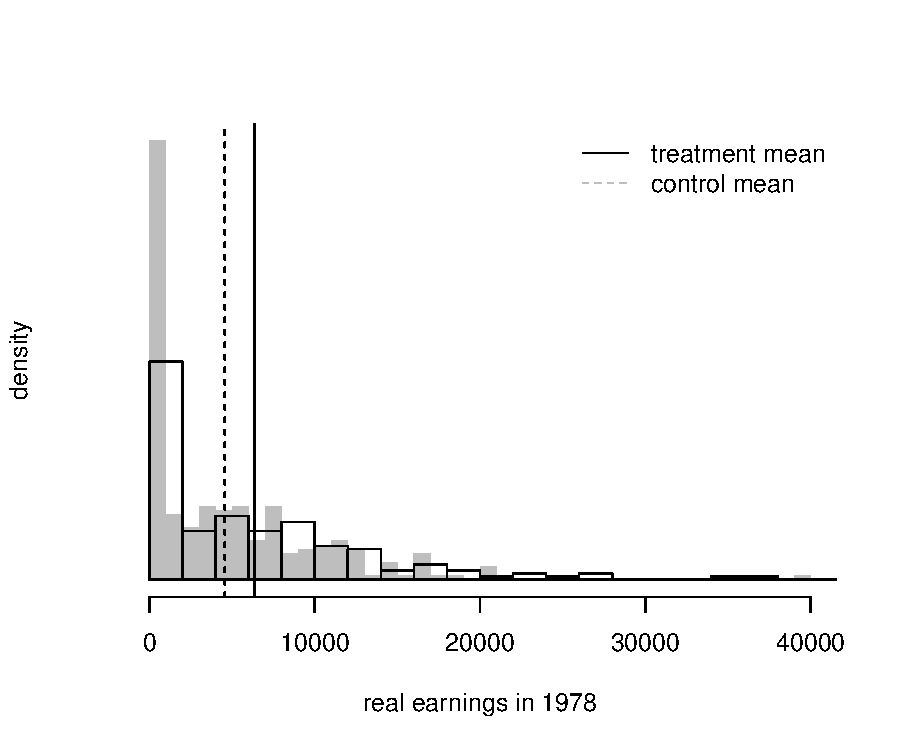
\includegraphics[width =  \textwidth]{figures/lalonde_histograms.pdf}
\caption{拉隆德实验数据中处理组（白色）与对照组（灰色）的收入分布直方图；垂直线分别为两组样本均值：实线为处理组，虚线为对照组。}\label{fig::lalonde-histograms}
\end{figure}



下述代码计算了四种典型统计量的观测值：
\begin{lstlisting}
> tauhat = t.test(y[z == 1], y[z == 0], 
+                 var.equal = TRUE)$statistic
> tauhat
       t 
2.835321 
> student = t.test(y[z == 1], y[z == 0],
+                 var.equal = FALSE)$statistic
> student
       t 
2.674146 
> W = wilcox.test(y[z == 1], y[z == 0])$statistic
> W
      W 
27402.5 
> D = ks.test(y[z == 1], y[z == 0])$statistic
> D
        D 
0.1321206 
\end{lstlisting}

随机置换处理向量，即可得到检验统计量随机化分布的蒙特卡洛近似，结果分别存放在\ri{Tauhat}、\ri{Student}、\ri{Wilcox}和\ri{Ks}四个向量中。 
\begin{lstlisting}
> MC = 10^4
> Tauhat   = rep(0, MC)
> Student  = rep(0, MC)
> Wilcox   = rep(0, MC)
> Ks       = rep(0, MC)
> for(mc in 1:MC)
+ {
+   zperm       = sample(z)
+   Tauhat[mc]  = t.test(y[zperm == 1], y[zperm == 0], 
+                        var.equal = TRUE)$statistic 
+   Student[mc] = t.test(y[zperm == 1], y[zperm == 0], 
+                        var.equal = FALSE)$statistic
+   Wilcox[mc]  = wilcox.test(y[zperm == 1], 
+                             y[zperm == 0])$statistic 
+   Ks[mc]      = ks.test(y[zperm == 1], 
+                         y[zperm == 0])$statistic
+ }
\end{lstlisting}



基于 FRT 的单侧$p$值均小于 0.05： 
\begin{lstlisting}
> exact.pv = c(mean(Tauhat >= tauhat),
+              mean(Student >= student),
+              mean(Wilcox >= W),
+              mean(Ks >= D))
> round(exact.pv, 3)
[1] 0.002 0.002 0.006 0.040
\end{lstlisting}
也可以不使用蒙特卡洛方法，直接计算渐近$p$值，它们同样均小于 0.05： 
\begin{lstlisting}
> asym.pv = c(t.test(y[z == 1], y[z == 0], 
+                    var.equal = TRUE)$p.value, 
+             t.test(y[z == 1], y[z == 0], 
+                    var.equal = FALSE)$p.value,
+             wilcox.test(y[z == 1], y[z == 0])$p.value,
+             ks.test(y[z == 1], y[z == 0])$p.value)
> round(asym.pv, 3)
[1] 0.005 0.008 0.011 0.046
\end{lstlisting}

这些$p$值的差异既来自渐近近似，也来自\ri{t.test}和\ri{wilcox.test}默认进行双侧检验。为作公平比较，需要将前三个$p_\frt$乘以$2$。 


图\ref{fig::randomizationdistribution-lalonde}给出了四个检验统计量随机化分布的直方图及其观测值。虽然原始结果数据的分布远非正态分布（见图\ref{fig::lalonde-histograms}），前三个统计量的正态近似仍很好。一般而言，图\ref{fig::randomizationdistribution-lalonde}这样的图形能更清楚地展示检验尖锐零假设所需的信息。近期\citet{bind2020possible}甚至在论文标题中倡议：“只要可能，就报告 Fisher 精确$p$值，并展示其对应的零假设随机化分布。”我赞同这一建议。 

\begin{figure}[ht]
\centering 
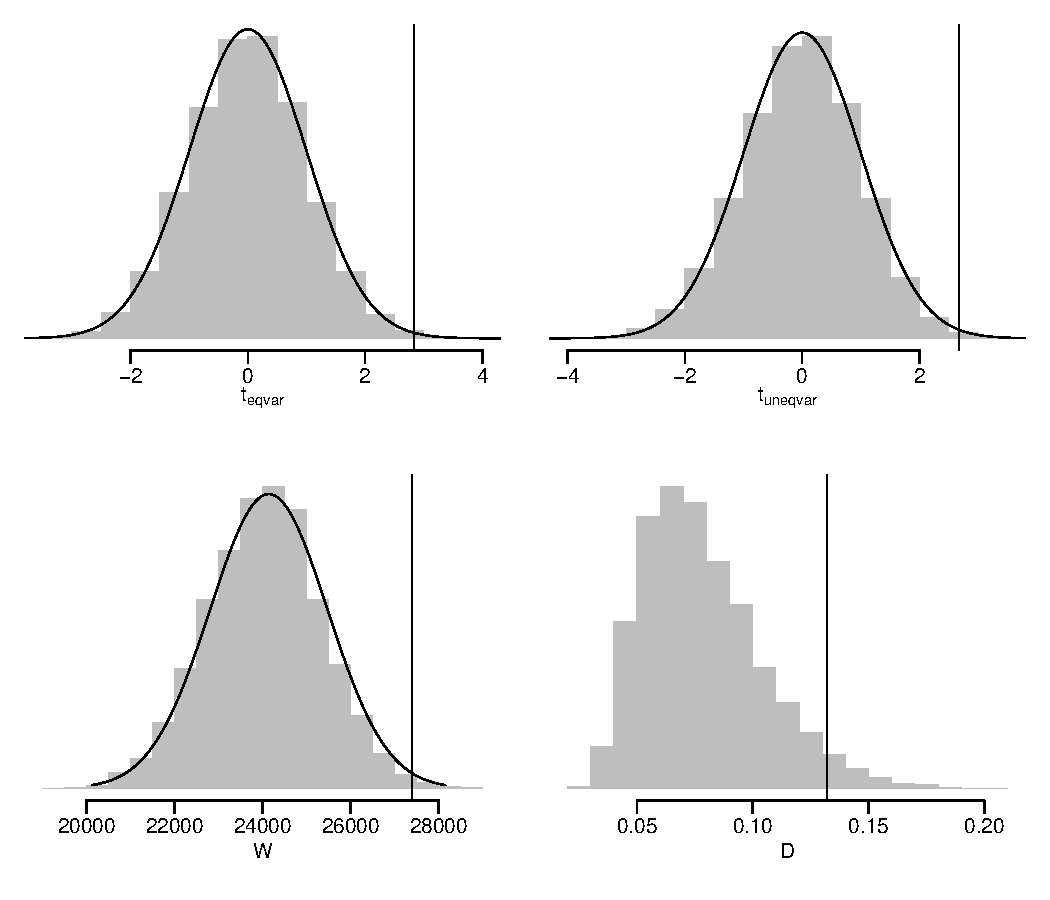
\includegraphics[width =  \textwidth]{figures/FRT_lalonde.pdf}
\caption{基于 LaLonde 实验数据的四个检验统计量的随机化分布} \label{fig::randomizationdistribution-lalonde}
\end{figure}





\section{随机实验与 FRT 的简史}


\subsection{James Lind 的实验}\label{section::lind}


James Lind（1716—1794）是一位苏格兰医生，也是英国皇家海军海上卫生研究的先驱。在他所处的时代，坏血病是水手死亡的主要原因之一。他开展了一项较早且细节记录清楚的随机实验，在维生素 C 被发现之前，就得出柑橘类水果能够治疗坏血病的结论。 


在\citet{lind1753treatise}中，他描述了将$12$名坏血病患者分到$6$组的随机实验。略去部分细节，$6$组分别为：
\begin{enumerate}
[(1)]
\item
两人每天饮用一夸脱苹果酒； 

\item
两人每天服用三次硫酸，每次二十五滴；

\item
两人每天服用三次醋，每次两匙；

\item
两人每天饮用半品脱海水；


\item
两人每天食用两个橙子和一个柠檬；

\item 
两人每天食用一种辛辣糊剂，并饮用大麦水。
\end{enumerate}

六天后，第五组患者康复，而其他组没有康复。若将处理简化为
$$
Z_i  = 1(\text{unit } i \text{ received citrus fruits})
$$
并将结果简化为
$$
Y_i = 1(\text{unit } i \text{ recovered after six days}),
$$
就得到如下二乘二列联表：

\begin{center}
\begin{tabular}{lcc}
\hline 
      & $Y =1$ & $Y =0$\\\hline
$Z =1$ & $2$ & $0$\\ 
$Z =0$ & $0$ & $10$\\
\hline 
\end{tabular}
\end{center}


这是该实验中能够观测到的最极端的二乘二列联表，数据为柑橘类水果治疗坏血病的正向效应提供了强有力的证据。从统计学角度，应如何衡量证据的强度？


按照 FRT 的逻辑，若处理完全没有效应（即$\HF$成立），如此极端的二乘二表出现的概率为
$$
 \frac{1}{\binom{12}{2}} = \frac{1}{66} = 0.015
$$
这就是$p_\frt$。在$\HF$下，这样的结果相当出乎意料：在$0.05.$水平上，我们很容易拒绝$\HF$。



\subsection{女士品茶}\label{section::lady-tasting-tea}


\citet{Fisher:1935}描述了著名的{\it 女士品茶}实验。\footnote{后来\citet{salsburg2001lady}撰写现代统计学史时，将这一名称用作书名。}一位女士声称，她能分辨两种制作奶茶的方法：先加奶和先加茶。多数人可能会觉得这个说法有些奇怪。作为统计学家，Fisher 设计了一项实验，检验这位女士是否真的能区分两种做法。 

他准备了$8$杯茶，其中$4$杯先加奶，另$4$杯先加茶，再将$8$杯茶按随机顺序呈给女士，请她选出先加奶的$4$杯。最终实验结果可汇总为下列二乘二表： 

\begin{tabular}{lccc}
\hline 
      &    先加奶（女士判断）&    先加茶（女士判断） & 列合计 \\ \hline
      先加奶（Fisher 安排） & $X$ & $4-X$ & 4\\ 
   先加茶（Fisher 安排） & $4-X$ & $X$ & 4\\
   行合计 & 4 & 4 &8 \\
   \hline 
\end{tabular}

$X$的可能取值为$0, 1, 2, 3, 4$。实际实验得到$X = 4$，这是最极端的数据，强烈表明女士确实能够区分两种奶茶做法。我们再次面临同一个问题：如何衡量证据的强度？


在女士无法区分两种做法的零假设下，$\binom{8}{4} = 70$种可能排列中，只有一种会得到$X=4$的二乘二表。因此，$p$值为
$$
p_\frt = \frac{1}{70} = 0.014.
$$
在$0.05$的显著性水平上，我们拒绝零假设。 



\subsection{Fisher 实验设计的两个原则}\label{sec::fisherian-principles-experiments}


在第\ref{section::lind}和\ref{section::lady-tasting-tea}节的两个例子中，$p_\frt$的有效性都由实验的随机化保证。这突出了 Fisher 实验设计的第一个原则：{\it 随机化}。




 
 
 


此外，从某种意义上说，上述两项实验已经是能够给出有统计意义结果的最小实验。例如，若 Lind 只给六个组各分配一名患者，则最小$p$值为
$$
\frac{1}{\binom{6}{1}}  =\frac{1}{6} = 0.167;
$$
若 Fisher 只准备$6$杯茶，其中$3$杯先加奶、另$3$杯先加茶，则最小$p$值为
$$
\frac{1}{\binom{6}{3}} = \frac{1}{20} = 0.05.
$$
此时无法在$0.05$水平上拒绝零假设。这突出了 Fisher 实验设计的第二个原则：{\it 重复}。也就是说，为使 FRT 具有检验功效，实验中必须有足够多的单位。 

 

第\ref{chapter::stratification-poststratification}章将讨论 Fisher 实验设计的第三个原则：{\it 区组化}。


 

 

\section{讨论}

\subsection{其他尖锐零假设与置信区间}\label{sec::frt-invert-interval}


上文着重讨论尖锐零假设$\HF$。实际上，FRT 的逻辑也适用于其他尖锐零假设。例如，对于已知向量$\bm{\tau} = (\tau_1, \ldots, \tau_n)$，可检验
$$
H_0(\bm{\tau}): Y_i(1) - Y_i(0) = \tau_i \text{ for all } i=1,\ldots, n
$$
在$H_0(\bm{\tau})$下，每个单位的因果效应都已知，因此可以根据观测数据填补所有缺失的潜在结果。潜在结果确定后，任意检验统计量$T = T(\bm{Z}, \bm{Y}(1), \bm{Y}(0))$的分布都完全由处理分配机制决定，从而可计算对应的$p_\frt$。它是$\bm{\tau} $的函数，记为$p_\frt(\bm{\tau} )$。若能列出所有可能的$\bm{\tau}$，就可得到一系列$p_\frt(\bm{\tau} )$。根据假设检验与置信集合的对偶性（见第\ref{section::duality-ci-testing}节），可构造平均因果效应的$(1-\alpha)$水平置信集合：
$$
\left \{ \tau = n^{-1}\sum_{i=1}^n \tau_i :  p_\frt(\bm{\tau} ) \geq \alpha \right \} .
$$
这个策略在概念上很直接，但所有可能的$\bm{\tau}$数量庞大，实践中存在计算困难。对于二元结果，\citet{Rigdon:2015}和\citet{li2016exact}提出了基于 FRT 构造$\tau$置信区间的可计算方法。对于一般无界结果，这一策略往往在计算上不可行。 


一种常用的简化\citep{rosenbaum2002design, Rosenbaum:2010}是只考虑个体因果效应恒定的一类尖锐零假设：
$$
H_0(c): Y_i(1) - Y_i(0) =  c\text{ for all } i=1,\ldots, n
$$
其中$c$是已知常数。给定$c$，可以计算$p_\frt(c)$。利用对偶性，可得到平均因果效应的$(1-\alpha)$水平置信集合：
$$
\{ c :  p_\frt(c ) \geq \alpha \} .
$$
这一过程只涉及一维搜索，因此在计算上可行。然而，个体因果效应恒定的假设过强。特别是，对于二元结果，只有所有单位的效应都为$0,$、都为$-1$或都为$1$时，该假设才能成立。一般而言，恒定个体因果效应假设对数据施加了可检验的限制，因此可能被观测数据拒绝；\citet{ding2015randomization}提出了正式的统计检验。 



\subsection{其他检验统计量}\label{section::other-statistic}


FRT 是一种一般性的策略，适用于任何随机实验和任何检验统计量。第\ref{sec::frt-choiceofstatistic}节已经介绍了若干统计量，其实统计量的定义还可以更一般。例如，令处理前协变量矩阵为$\bm{X}$，第$i$行为单位$i$的协变量$X_i$，$(i = 1, \ldots, n)$。\footnote{在因果推断中，只有不受处理影响的变量$X_i$才称为协变量。也就是说，若它有两个潜在结果$X_i(1)$和$X_i(0)$，则二者必须满足$X_i(1) = X_i(0)$。标准统计教材往往不区分处理与协变量，因为二者通常都出现在结果回归模型的右侧，并都被称为协变量。本书加以区分，因为它们在因果推断中发挥不同作用。}此时可以令检验统计量$T(\bm{Z}, \bm{Y}, \bm{X})$为处理向量、结果向量和协变量矩阵的函数，习题\ref{hw::frt-covariates}给出了一个例子。 



\subsection{最后的说明}对于一般的实验，$\bm{Z}$未必在所有由$n_1$个 1 和$n_0$个 0 构成的排列上均匀分布，但实验者完全知道其分布。因此，总能模拟该分布，进而得到尖锐零假设下任意检验统计量的分布。有限样本精确$p$值为
$$
p_\textsc{frt} = \pr'\{  T(\bm{Z}', \bm{Y}) \geq T(\bm{Z}, \bm{Y}) \}
$$
其中$\pr'$表示在给定数据后，对$\bm{Z}'$的分布求平均。后续章节将讨论其他实验。这里强调，FRT 的适用范围不限于本书介绍的几种具体实验。 

 
FRT 可以使用任意检验统计量，但这并未回答实际分析中应如何选择统计量。如果目的是发现与尖锐零假设不相容的结果，就应选择在备择假设下功效较高的统计量。一般没有一种统计量的功效能始终优于其他统计量，因为功效取决于备择假设。第\ref{sec::frt-choiceofstatistic}节的四个统计量针对不同备择假设：例如，$\hat{\tau}$和$t$针对平均处理效应不为零的备择；$W$则针对结果呈重尾分布、因果效应恒定的备择。指定一个工作备择假设通常有助于构造检验统计量，但 FRT 的有效性并不要求该备择假设准确。习题\ref{hw::frt-covariates}和\ref{hw::frt-glm}说明了如何利用工作备择假设或统计模型构造统计量。 
 



\section{作业习题}



\paragraph{$p_\frt$的精确性}
\label{hw::exact-frt}

证明 \eqref{eq::p-value-valid}。 



\paragraph{$\hat p_\frt$的蒙特卡洛误差}\label{para::monte-carlo-error-pfrt}

给定数据后，$p_\frt$是固定数，而它在\eqref{eq::mcpvalue}中的蒙特卡洛估计$\hat p_\frt$仍是随机的。证明
$$
E_{\text{mc}} (\hat p_\frt) =   p_\frt
$$
以及
$$
\var_{\text{mc}} (\hat p_\frt)  \leq \frac{1}{4R},
$$
下标“mc”表示蒙特卡洛方法引入的随机性：$\hat p_\frt$之所以随机，是因为各$\bm{z}^r$是从$\bm{Z}$的所有可能取值中独立随机抽取的$R$个向量。


注：$p_\frt$的随机性来自$\bm{Z}$，但本题以数据为条件，故$p_\frt$成为固定数。$\hat p_\frt$的随机性则来自各$\bm{z}^r$是$\bm{Z}$的随机置换。习题\ref{para::monte-carlo-error-pfrt}证明，对蒙特卡洛随机性求平均时，$\hat p_\frt$是$p_\frt$的无偏估计量，并给出了$\hat p_\frt$方差的上界。\citet[][Theorem 2]{luo2021leveraging}给出了更精细的蒙特卡洛误差界。




\paragraph{$p_\frt$的有限样本有效蒙特卡洛近似}\label{para::finite-sample-exact-monte-carlo-frt}


尽管由习题\ref{para::monte-carlo-error-pfrt}可知$\hat p_\frt$是$p_\frt$的无偏估计量，但当$R$有限时，蒙特卡洛误差可能使它不满足对所有$u\in (0,1)$都有$\pr(\hat p_\frt \leq u) \leq u$的要求，因而未必是有效$p$值。下面的修正蒙特卡洛近似始终是有限样本有效的$p$值。\citet{phipson2010permutation}在置换检验中指出了这一技巧。



定义
$$
\tilde p_\frt  =  \frac{  1 + \sum_{r=1}^R   I\{ T(\bm{z}^r,\bm{Y})   \geq T(\bm{Z},\bm{Y})   \}  }{1+R}
$$
其中各$\bm{z}^r$是$\bm{Z}$的$R$次随机置换。证明：无论$R$取何值，蒙特卡洛近似$\tilde p_\frt $始终是有限样本有效的$p$值，即对所有$u\in (0,1)$均有$\pr(\tilde p_\frt \leq u) \leq u$。


 
注：可利用以下两个基本概率结论证明习题\ref{para::finite-sample-exact-monte-carlo-frt}的结论。 


\begin{lemma}
\label{lemma::binomial-order}
设两个二项随机变量$X_1\sim \text{Binomial}(R, p_1)$和$X_2\sim \text{Binomial}(R, p_2)$满足$p_1\geq p_2$，则对所有$x.$，均有$\pr(X_1\leq x) \leq  \pr(X_2\leq x) $。
\end{lemma}

\begin{lemma}
\label{lemma::uniform}
若$p\sim \text{Uniform}(0,1)$且$X\mid p \sim \text{Binomial}(R, p)$，则从边际分布来看，$X$在$\{ 0,1,\ldots, R  \}$上服从均匀分布。 
\end{lemma}

 


\paragraph{费舍尔精确检验}
\label{hw::frt-fisherexacttest}

考虑结果为二元变量的完全随机实验，将数据汇总为以下二乘二表：
 \begin{center}
\begin{tabular}{lccc}
\hline 
        & $Y =1$ & $Y =0$& 合计\\\hline
$Z =1$ & $n_{11}$ & $n_{10}$ & $n_1$\\ 
$Z =0$ & $n_{01}$ & $n_{00}$ & $n_0$\\ 
\hline 
\end{tabular}
\end{center}
在$\HF$下，证明任意检验统计量$T(n_{11}, n_{10}, n_{01}, n_{00})$都是$n_{11}$与其他非随机常数的函数，且$n_{11}$的精确分布为超几何分布。写出该超几何分布的参数。 

注：\citet{barnard1947significance}和\citet{Ding:2015}指出，在具有二元结果的完全随机实验中，Fisher 精确检验（见第\ref{sec::fisher-exact-test}节）与 FRT 等价。 





\paragraph{女士品茶实验的更多细节}
\label{hw::more-tea}

回顾第\ref{section::lady-tasting-tea}节的例子。计算$k=0,1,2,3,4$时的$\pr(X=k)$。 


\paragraph{协变量调整后的 FRT}
\label{hw::frt-covariates}


本题补充第\ref{section::other-statistic}节的细节。  


第\ref{sec::frt-lalonde-experiment}节使用四种检验统计量，通过 FRT 重新分析了 LaLonde 实验数据。若有额外协变量，至少还可以采用以下两种策略，使 FRT 更一般。假定所有潜在结果和协变量均为固定数。 

第一种策略是使用基于线性回归残差的检验统计量。将结果对协变量作线性回归，得到残差，并把残差视为“伪结果”。然后用残差定义前述四种统计量，分别实施 FRT，报告相应的$p$值。


第二种策略是将结果对处理和协变量作线性回归，以处理的回归系数作为检验统计量实施 FRT，并报告相应$p$值。 


为什么上述两种策略给出的五个$p$值都具有有限样本精确性？请说明理由。 



\paragraph{使用广义线性模型的 FRT}
\label{hw::frt-glm}


使用习题\ref{hw::frt-covariates}的数据集，将结果改为表示\ri{re78}是否为正的二元指标。将结果对处理与协变量作逻辑回归。处理系数是否显著？对应的$p$值是多少？再以处理系数作为检验统计量，计算 FRT 的$p$值。 




\paragraph{一个代数细节}
\label{hw::frt-algebraic-detail}

验证 \eqref{eq::frt-algebra-difference-in-means}。 



\paragraph{推荐阅读}

近期论文\citet{bind2020possible}倡导在分析复杂实验时，同时报告$p$值并展示相应的随机化分布。 


  
\chapter{完全随机实验中的内曼重复抽样推断}\label{chapter::neyman-cr}
 \chaptermark{完全随机实验与内曼推断}
 
 
在具有里程碑意义的论文中，\citet{Neyman:1923}不仅提出了潜在结果的概念，还推导出了在完全随机实验条件下对平均因果效应进行推断的严格数学结论。与费希尔在尖锐零假设下计算$p$值的思想不同，\citet{Neyman:1923}提出了一种无偏点估计量，以及基于该估计量抽样分布得到的保守置信区间。本章将介绍\citet{Neyman:1923}的这些基础性结论，它们对于理解本书\ref{part::rcts}部分后续章节至关重要。



\section{有限总体中的统计量}

考虑包含$n$个单位的完全随机实验，其中$n_1$个接受处理，$n_0$个作为对照。单位$i = 1, \ldots, n$的潜在结果为$Y_i(1)$和$Y_i(0)$，个体效应为$\tau_i = Y_i(1) - Y_i(0).$。潜在结果的有限总体均值为
$$
\bar{Y}(1) = n^{-1} \sumn Y_i(1),\quad
\bar{Y}(0) = n^{-1} \sumn Y_i(0),
$$
方差为\footnote{以$n-1$为除数可使本章主要定理更简洁。改用$n$会使公式复杂，但不改变基本结论；$n$较大时，差异很小。}
$$
S^2(1) = (n-1)^{-1} \sumn \{ Y_i(1) -\bar{Y}(1)  \}^2,\quad
S^2(0) = (n-1)^{-1} \sumn \{ Y_i(0) -\bar{Y}(0)  \}^2 ,
$$
协方差为
$$
S(1,0) = (n-1)^{-1} \sumn \{ Y_i(1) -\bar{Y}(1)  \}\{ Y_i(0) -\bar{Y}(0)  \} . 
$$
个体效应的均值为
$$
\tau = n^{-1} \sumn \tau_i = \bar{Y}(1) - \bar{Y}(0) .
$$
方差为
$$
S^2(\tau) = (n-1)^{-1} \sumn (\tau_i - \tau)^2.
$$
这些方差与协方差满足以下关系。
\begin{lemma}\label{lemma::variancecovariancetau}
$2S(1,0) = S^2(1)+S^2(0) - S^2(\tau).$
\end{lemma}

引理\ref{lemma::variancecovariancetau}是后续讨论要用到的基本结论。引理\ref{lemma::variancecovariancetau}可通过初等代数证明，留作习题\ref{hw::proof-covariance-basic}。 

这些统计量均由科学表$\{ Y_i(1), Y_i(0)  \}_{i=1}^n$所决定。我们感兴趣的是：基于完全随机实验中观测到的数据$ (Z_i, Y_i)_{i=1}^n$，如何估计平均因果效应$\tau$。 


\section{\citet{Neyman:1923}的定理}


根据观测结果，可计算样本均值
$$
\hat{\bar{Y}}(1) = n_1^{-1} \sumn Z_i Y_i,\quad
\hat{\bar{Y}}(0) = n_0^{-1} \sumn (1-Z_i) Y_i,
$$
与样本方差
$$
\hat{S}^2(1) = (n_1 - 1)^{-1} \sumn Z_i  \{  Y_i - \hat{\bar{Y}}(1) \}^2,\quad
\hat{S}^2(0) = (n_0 - 1)^{-1} \sumn (1-Z_i)  \{  Y_i - \hat{\bar{Y}}(0) \}^2 . 
$$
但$S(1,0)$与$S^2(\tau)$没有可计算的样本版本，因为每个单位$i$的潜在结果$Y_i(1)$和$Y_i(0)$永远不能同时观测。\citet{Neyman:1923}证明了以下定理。 




\begin{theorem}
\label{thm::neyman1923}
在完全随机实验条件下， 
\begin{enumerate}
\item
均值差估计量$\hat{\tau} =\hat{\bar{Y}}(1) -  \hat{\bar{Y}}(0)$是$\tau$的无偏估计量：
$$
E(\hat{\tau}) =\tau ;
$$ 
\item
$\hat{\tau} $的方差为
\begin{eqnarray}
\var(\hat{\tau})  &=&  \frac{S^2(1)}{n_1} + \frac{S^2(0)}{n_0} - \frac{S^2(\tau)}{n} \label{eq::neyman23var} \\
&=& \frac{n_0}{n_1 n} S^2(1) + \frac{n_1}{n_0 n} S^2(0) + \frac{2}{n} S(1,0) ;  \label{eq::neyman23var-equivalent}
\end{eqnarray}
\item\label{neyman-3}
方差估计量 
$$
\hat{V} = \frac{\hat{S}^2(1)}{n_1} + \frac{\hat{S}^2(0)}{n_0}
$$
是$\var(\hat{\tau})$的一个保守估计量，即满足
$$
E(\hat{V} ) - \var(\hat{\tau})  = \frac{S^2(\tau)}{n}  \geq 0
$$
当且仅当所有单位的$\tau_i = \tau$时等号成立。 
\end{enumerate}
\end{theorem}

定理\ref{thm::neyman1923}的证明见第\ref{sec::prove-neyman-1923}节。在证明定理\ref{thm::neyman1923}之前，必须澄清定理\ref{thm::neyman1923}中$E(\cdot)$与$\var(\cdot)$的含义。潜在结果均固定，只有处理指标$Z_i$随机。因此，期望与方差都针对各$Z_i$的随机性计算；处理向量是$n_1$个 1 与$n_0$个 0 的随机排列。图\ref{fig::neyman1923}说明$\hat\tau$的随机性：$M=\binom{n}{n_1}$种处理分配等概率出现，分别对应$\{ \hat\tau^1 , \ldots, \hat\tau^M\}$中的取值，从而诱导其抽样分布。比较图\ref{fig::neyman1923}与图\ref{fig::frt}，可见 FRT 与\citet{Neyman:1923}定理的关键区别：
\begin{enumerate}
\item
FRT 适用于任意检验统计量，\citet{Neyman:1923}的定理则只针对均值差。虽然也可为其他估计量推导类似\citet{Neyman:1923}的结论，但对一般估计量而言，数学推导往往很困难。 

\item
图\ref{fig::frt}中观测结果向量$\bm{Y}$是固定不变的，而图\ref{fig::neyman1923}中$\bm{Y}(\bm{z}^m)$的值随处理分配方案$\bm{z}^m$变化。 

\item
图\ref{fig::frt}中各$T(\bm{z}^m,\bm{Y}) $均可由观测数据计算，图\ref{fig::neyman1923}中各$\hat\tau^m$却是假想值，因为并非所有潜在结果都已知。 
\end{enumerate}

\begin{figure}[ht]
\centering 
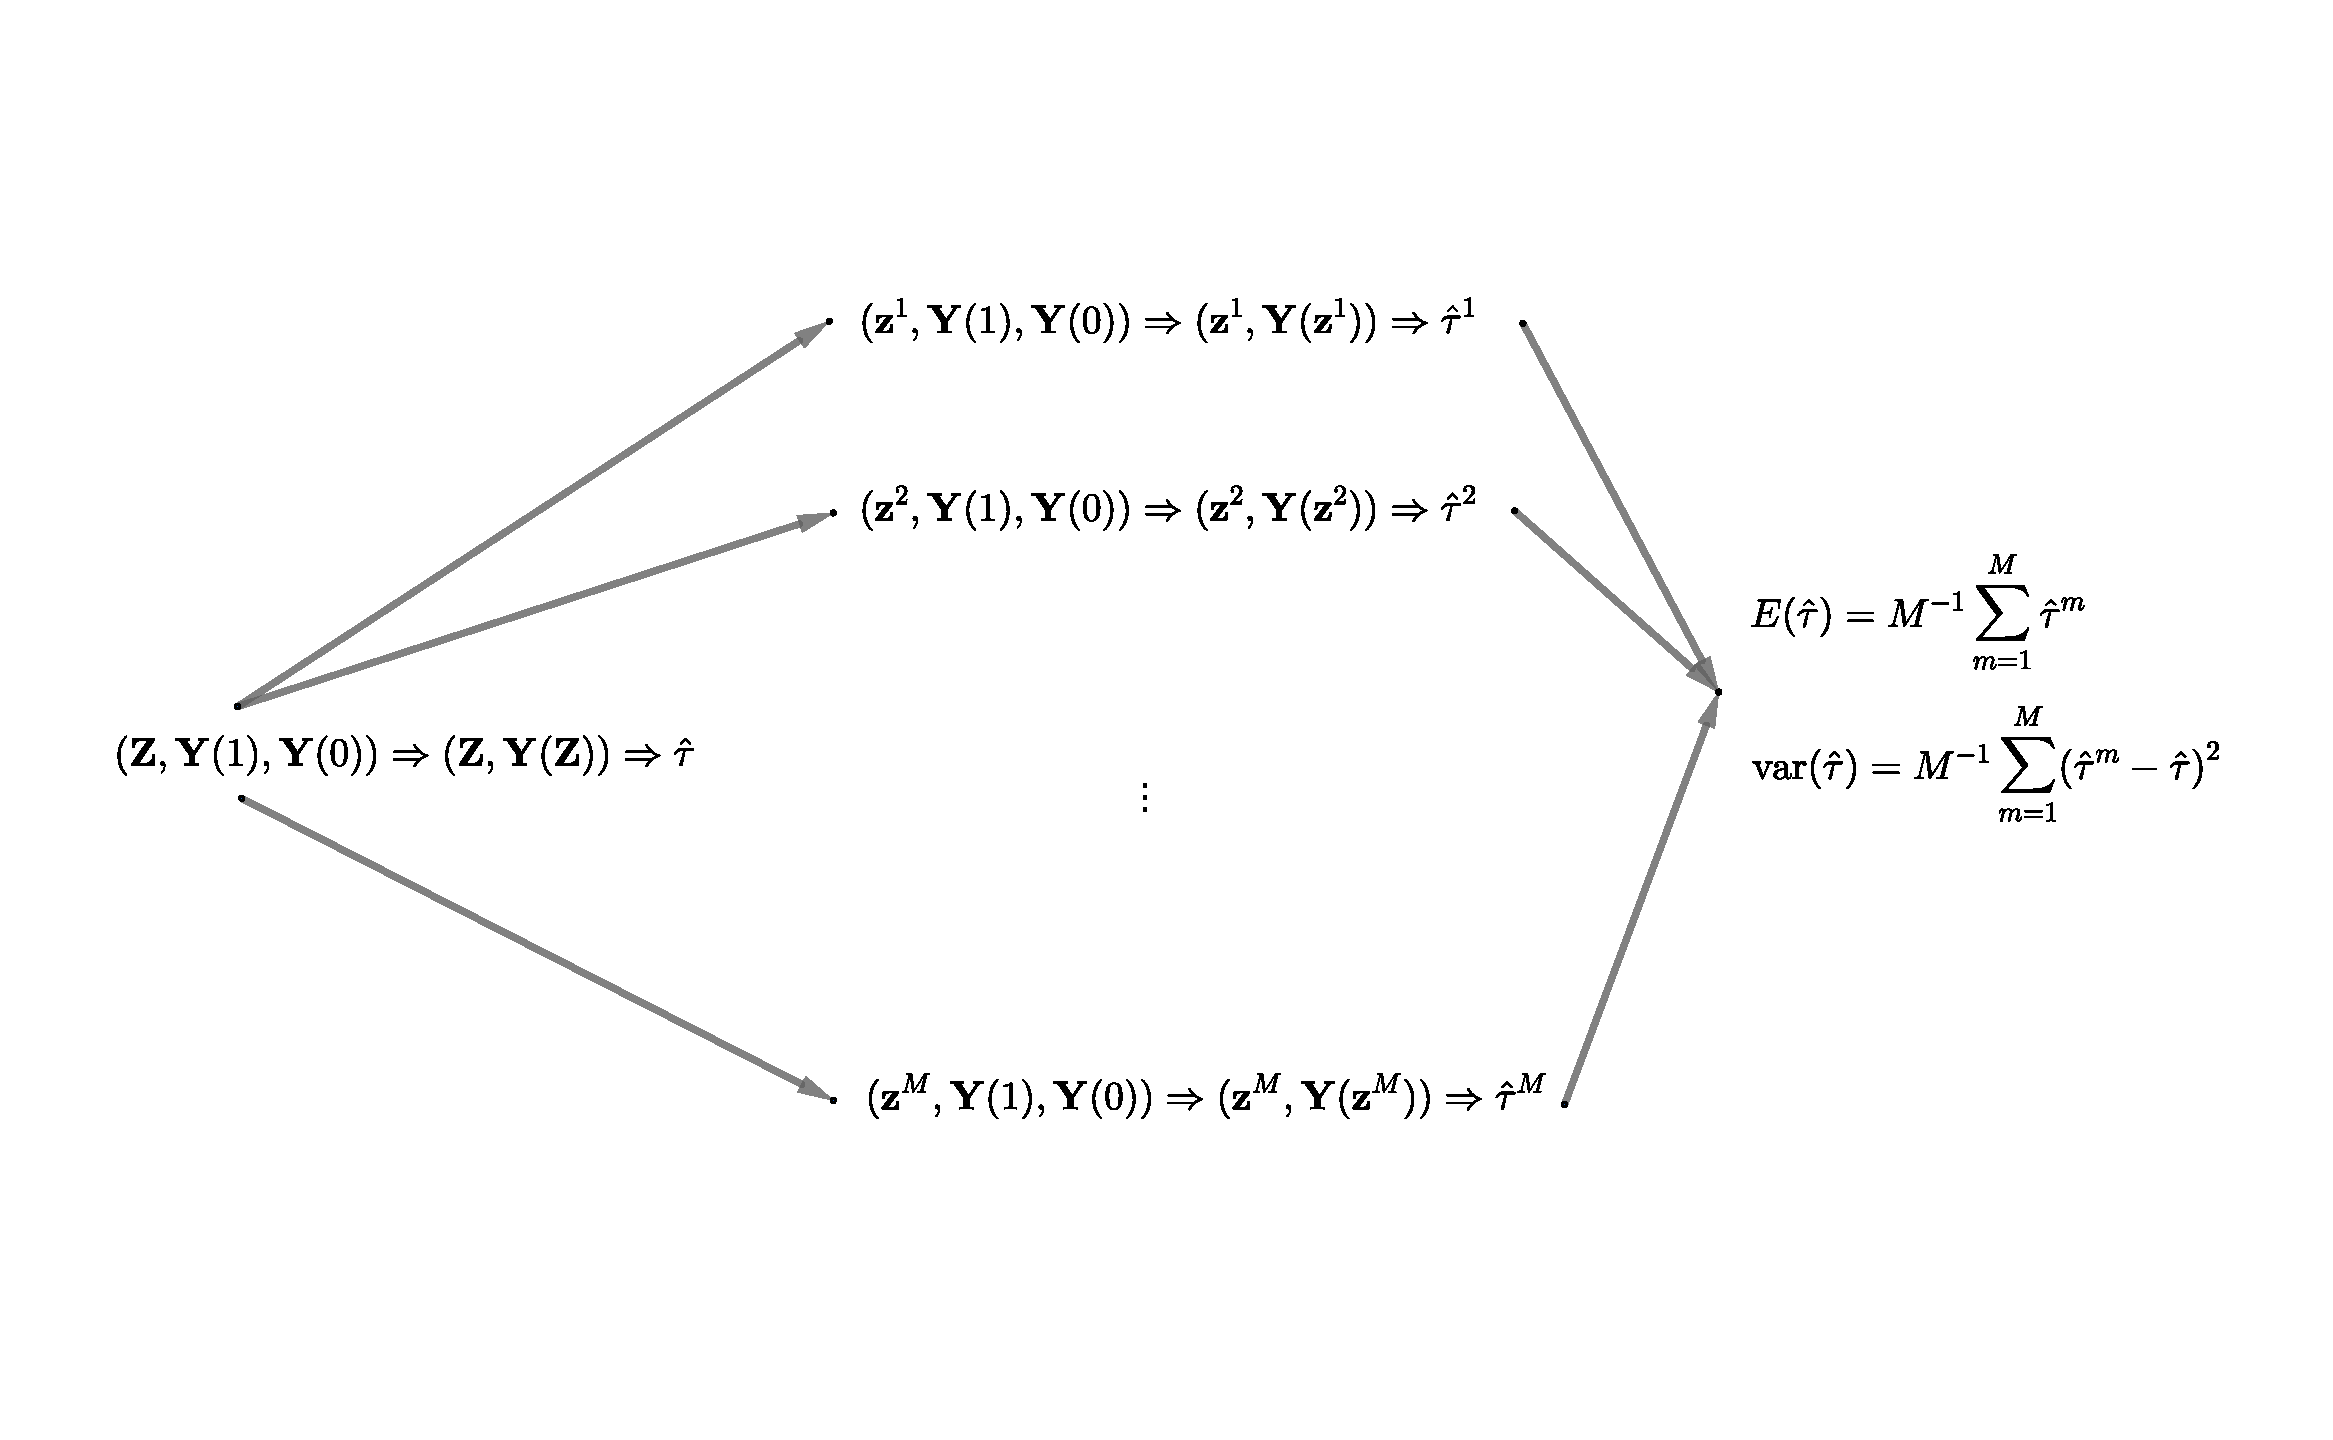
\includegraphics[width =  \textwidth]{figures/neyman1923_fig.pdf}
\caption{\citet{Neyman:1923}定理示意图，其中$\bm{Y}(\bm{z}^m)$为给定处理分配方案$\bm{z}^m$时的观测结果向量。}\label{fig::neyman1923}
\end{figure}




点估计量$\hat\tau$虽然形式简单，但在完全随机实验框架下其方差却具有非平凡特性。式\eqref{eq::neyman23var}所示的方差表达式与经典均值差方差公式\footnote{在经典双样本问题中，处理组观测值独立同分布于均值$\mu_1$、方差$\sigma_1^2$的分布，对照组观测值独立同分布于均值$\mu_0$、方差$\sigma_0^2$的分布。此时有
$$
\var(\hat{\tau} ) = \frac{\sigma_1^2}{n_1} +  \frac{\sigma_0^2}{n_0}.
$$
此处$\var(\cdot)$均指观测值的随机性。该公式不含涉及个体因果效应方差的第三项。}存在显著差异：它不仅取决于潜在结果的有限总体方差，还包含个体处理效应方差（或等价的潜在结果协方差）。遗憾的是，由于$Y_i(1)$与$Y_i(0)$无法同时观测，因此$S^2(\tau)$与$S(1,0)$均无法由数据直接识别。 




公式\eqref{eq::neyman23var}有些令人困惑：个体效应越异质，$\hat{\tau}$的变异反而越小。第\ref{sec::simulation-neyman-formula}节将用数值例子验证\eqref{eq::neyman23var}。直观原因是什么？可以根据等价形式\eqref{eq::neyman23var-equivalent}，比较潜在结果正相关与负相关的情形。处理组虽然是从$n$个单位的有限总体中简单随机抽取的，一次实际实验仍可能恰好选到处理潜在结果较大的单位。假设出现了这种情况。 
\begin{enumerate}
\item
若$S(1,0) > 0$，这些处理单位的对照潜在结果也较大，剩余对照单位的观测结果因而较小，使$\hat\tau$较大。 
\item
若$S(1,0) < 0$，这些处理单位的对照潜在结果较小，剩余对照单位的观测结果因而较大，使$\hat\tau$较小。 
\end{enumerate}
若某次实验恰好选到处理潜在结果较小的单位，也会出现方向相反的情况。总之，$\hat\tau$的无偏性不依赖潜在结果的相关性，但与$S(1,0) < 0$相比，在$S(1,0) > 0$下更容易观测到极端的$\hat\tau$。因此，潜在结果正相关时，$\hat{\tau}$的方差更大。 

 
 
 
 


\citet[][Theorem 5 and Proposition 3]{li2017general}基于有限总体中心极限定理，进一步证明了$\hat{\tau}$的以下渐近正态性。
\begin{theorem}
\label{thm::clt-difference-in-means}
设$n\rightarrow \infty$且$n_1 \rightarrow \infty$。若$n_1/n$收敛于$(0,1)$区间内的某定值，$\{S^2(1), S^2(0), S(1,0)\}$亦存在极限值，且满足
$$  
\max_{1\leq i \leq n}\{ Y_i(1) - \bar{Y}(1) \}^2/n \rightarrow 0, \quad 
\max_{1\leq i \leq n}\{ Y_i(0) - \bar{Y}(0) \}^2/n \rightarrow 0,
$$
则
$$
\frac{   \hat{\tau} - \tau }{  \sqrt{ \var(\hat{\tau}) } } \rightarrow \N01
$$
依分布收敛，同时
$$
\hat{S}^2(1) \rightarrow S^2(1),\quad 
\hat{S}^2(0) \rightarrow S^2(0)
$$
依概率收敛。 
\end{theorem}


定理\ref{thm::clt-difference-in-means}的证明涉及较多技术细节，超出本书范围。它保证在大样本及一定正则条件下，$\hat{\tau} $的抽样分布可用正态分布近似；结果的样本方差也一致估计总体方差，从而使\cite{Neyman:1923}方差估计的概率极限不低于$\hat{\tau} $的真实方差。因此，可构造$\tau$的保守大样本置信区间：
$$
\hat{\tau} \pm z_{1-\alpha/2} \sqrt{  \hat{V}  },
$$
其中$z_{1-\alpha/2}$为标准正态分布的$1-\alpha/2$分位数。这与标准双样本问题的置信区间渐近相同（见第\ref{sec::bf-problem}节）。样本量足够大时，该区间覆盖$\tau$的概率至少为$1-\alpha$。由对偶性，可据此检验
$$
\HN: \tau = 0,
$$
这称为弱零假设。 



由于潜在结果缺失的根本性限制，我们只能获得保守型方差估计量。统计学中置信区间的定义本身即允许覆盖率超标的存在，这也使得方差估计的保守性具有合理性（参见\ref{sec::statistical-inference}节）。若实际研究中对处理效应估计不足的危害可控，这种保守性便无大碍。但当研究涉及药物副作用测量时，估计不足可能带来严重危害——例如新药的毒性效应若被低估将危及患者健康。 
 
 

\section{证明}\label{sec::prove-neyman-1923}

本节将完整证明定理\ref{thm::neyman1923}。


首先，$\hat{\tau}$的无偏性可直接由如下展开式与期望线性性质推导：
\begin{eqnarray*}
\hat{\tau} &=& n_1^{-1} \sumn Z_i Y_i - n_0^{-1} \sumn (1-Z_i) Y_i \\
&=& n_1^{-1} \sumn Z_i Y_i(1) - n_0^{-1} \sumn (1-Z_i) Y_i(0) 
\end{eqnarray*}
于是
\begin{eqnarray*}
E( \hat{\tau}  ) &=& E\left\{    n_1^{-1} \sumn Z_i Y_i(1) - n_0^{-1} \sumn (1-Z_i) Y_i(0)   \right\} \\
&=& n_1^{-1} \sumn E(Z_i) Y_i(1) - n_0^{-1} \sumn E(1-Z_i) Y_i(0) \\
&=& n_1^{-1} \sumn \frac{n_1}{n} Y_i(1) - n_0^{-1} \sumn \frac{n_0}{n} Y_i(0) \\
&=&  n^{-1} \sumn Y_i(1) - n^{-1} \sumn Y_i(0) \\
&=& \tau .
\end{eqnarray*}


第二，将$\hat{\tau}$进一步改写为
\begin{eqnarray*}
\hat{\tau} &=&  \sumn Z_i  \left\{    \frac{  Y_i(1) }{ n_1 } + \frac{  Y_i(0) }{ n_0 }   \right\}
- n_0^{-1} \sumn Y_i(0).
\end{eqnarray*}
根据简单随机抽样的引理\ref{lemma::samplemean}，$\hat{\tau}$的方差为
\begin{eqnarray*}
\var(\hat{\tau}) &=&  \frac{  n_1 n_0  }{  n(n-1)  }  \sumn  
\left\{    \frac{  Y_i(1) }{ n_1 } + \frac{  Y_i(0) }{ n_0 }  -  \frac{  \bar{Y}(1) }{ n_1 } - \frac{  \bar{Y}(0) }{ n_0 }    \right\}^2 \\
&=&  \frac{  n_1 n_0  }{  n(n-1)  }  \left[
\frac{1}{n_1^{2}}   \sumn  \{  Y_i(1) -  \bar{Y}(1)\}^2 + \frac{1}{n_0^{2}}  \sumn  \{  Y_i(0) -  \bar{Y}(0)\}^2 \right. \\
&& \left. \qquad \qquad 
+ \frac{2}{n_1 n_0}  \sumn  \{  Y_i(1) -  \bar{Y}(1)\}  \{  Y_i(0) -  \bar{Y}(0)\} 
\right]\\
&=& \frac{n_0}{n_1n} S^2(1) + \frac{n_1}{n_0n}S^2(0) + \frac{2}{n} S(1,0). 
\end{eqnarray*}
由引理\ref{lemma::variancecovariancetau}，还可将方差写为
\begin{eqnarray*}
\var(\hat{\tau})
&=& \frac{n_0}{n_1n} S^2(1) + \frac{n_1}{n_0n}S^2(0) + \frac{1}{n} \{ S^2(1)+S^2(0) - S^2(\tau) \}\\
&=&  \frac{S^2(1)}{n_1} + \frac{S^2(0)}{n_0} - \frac{S^2(\tau)}{n}.
\end{eqnarray*}

第三，处理组是从$n$个单位中抽取的大小为$n_1$的简单随机样本。因此，由引理\ref{lemma::variance-unbiased}，各$Y_i(1)$的样本方差无偏估计总体方差：
$$
E\{  \hat{S}^2(1) \} = S^2(1).
$$
类似地，$E\{  \hat{S}^2(0) \} = S^2(0).$。所以$\hat{V} $是\eqref{eq::neyman23var}前两项之和的无偏估计。 
 
 
 
 
 \section{完全随机实验的回归分析}
 
 
 
实践中常用回归对平均因果效应$\tau$作推断。标准做法是将结果对处理指标及截距作普通最小二乘（OLS）回归：
$$
(\hat\alpha, \hat\beta) = \arg\min_{(a,b)} \sum_{i=1}^n (Y_i - a - bZ_i)^2,
$$
以处理系数$ \hat\beta$估计平均因果效应。可以证明，$ \hat\beta$恰好等于均值差：
\begin{equation}
\label{eq::ols-difference-in-means}
\hat\beta = \hat\tau .
\end{equation}

但 OLS 的通常方差估计量（见第\ref{appendix::basic-linear-regression}章的\eqref{eq::v-hat-ols}），例如\ri{R}中\ri{lm}函数的输出，等于
\begin{eqnarray}
\label{eq::ols-se}
\hat V_\textsc{ols} &=& \frac{n\left(n_1 -1\right)}{( n-2 ) n_1  n_0 } \hat S^2(1) +\frac{n\left(n_0 -1\right)}{( n-2 ) n_1  n_0 } \hat S^2(0)\\
\nonumber &\approx& \frac{\hat S^2(1)}{n_0 }+\frac{ \hat S^2(0) }{n_1 },
\end{eqnarray}
近似在$ n_1 $和$ n_0 $较大时成立。即使$ n_1 $、$ n_0 $很大，它仍不同于$\hat{V}$。 


幸运的是，Eicker--Huber--White（EHW）稳健方差估计量（见第\ref{appendix::basic-linear-regression}章的\eqref{eq::v-hat-ehw}）接近$\hat{V}$：
\begin{eqnarray}
\label{eq::ols-ehw}
\hat V_\textsc{ehw} &=& \frac{\hat S^2(1)}{n_1 } \frac{n_1 -1}{n_1 }+\frac{\hat S^2(0)}{n_0 } \frac{n_0 -1}{n_0 } \\
\nonumber &\approx& \frac{ \hat S^2(1)  }{n_1 }+\frac{ \hat S^2(0) }{n_0 }
\end{eqnarray}
近似在$ n_1 $和$ n_0 $较大时成立，几乎等于$\hat{V}$。而且，EHW 稳健方差估计的 HC2 变体与$\hat{V}$完全相同。\ri{car}包中的\ri{hccm}函数可以计算 EHW 稳健方差及 HC2 变体。 

习题\ref{hw::neyman-ols-nox}给出了\eqref{eq::ols-difference-in-means}至\eqref{eq::ols-ehw}的更多技术细节。 
 



 

 
\section{实例演示} 


\subsection{模拟}
\label{sec::simulation-neyman-formula}



首先设定样本总量$n=100$，其中处理组$60$例、对照组$40$例，生成个体效应恒定的潜在结果： 
\begin{lstlisting}
n  = 100
n1 = 60
n0 = 40
y0 = rexp(n)
y0 = sort(y0, decreasing = TRUE)
y1 = y0 + 1
 \end{lstlisting}
固定科学表，反复生成完全随机实验，并应用定理\ref{thm::neyman1923}计算点估计、保守方差估计以及基于正态近似的置信区间。图\ref{fig::simulation-neyman}的$(1,1)$子图给出潜在结果散点图，图\ref{fig::simulation-neyman}的$(1,2)$子图给出$\hat{\tau} - \tau$的直方图。 

随后反转对照组结果顺序重新模拟：
\begin{lstlisting}
y0 = sort(y0, decreasing = FALSE)
 \end{lstlisting}
并重复上述模拟。图\ref{fig::simulation-neyman}的$(2,1)$子图给出潜在结果散点图，图\ref{fig::simulation-neyman}的$(2,2)$子图给出$\hat{\tau} - \tau$的直方图。 




最后，随机置换对照潜在结果： 
 \begin{lstlisting}
y0 = sample(y0)
 \end{lstlisting}
 并重复上述模拟。图\ref{fig::simulation-neyman}的$(3,1)$子图给出潜在结果散点图，图\ref{fig::simulation-neyman}的$(3,2)$子图给出$\hat{\tau} - \tau$的直方图。 

 
 三组模拟中，潜在结果的相关性不同，但边际分布相同。下表比较真实方差、估计方差的平均值以及$95\%$置信区间的覆盖率。 
 \begin{lstlisting}
              constant negative independent
var              0.036    0.007       0.020
estimated var    0.036    0.036       0.036
coverege rate    0.947    1.000       0.989
 \end{lstlisting}
真实方差依赖潜在结果的相关性：潜在结果正相关时，抽样方差较大，验证了\eqref{eq::neyman23var-equivalent}。估计方差几乎相同，因为$\hat{V}$的公式只依赖潜在结果的边际分布。由于真实方差与估计方差不同，三组模拟的覆盖率也不同。只有因果效应恒定时，估计方差才在平均意义上等于真实方差，验证了定理\ref{thm::neyman1923}的第\ref{neyman-3}点。 
 
图\ref{fig::simulation-neyman}还画出了基于$\hat{\tau} $中心极限定理的正态密度曲线，与模拟直方图很接近，验证了定理\ref{thm::clt-difference-in-means}。
 
 
 \begin{figure}
 \centering 
 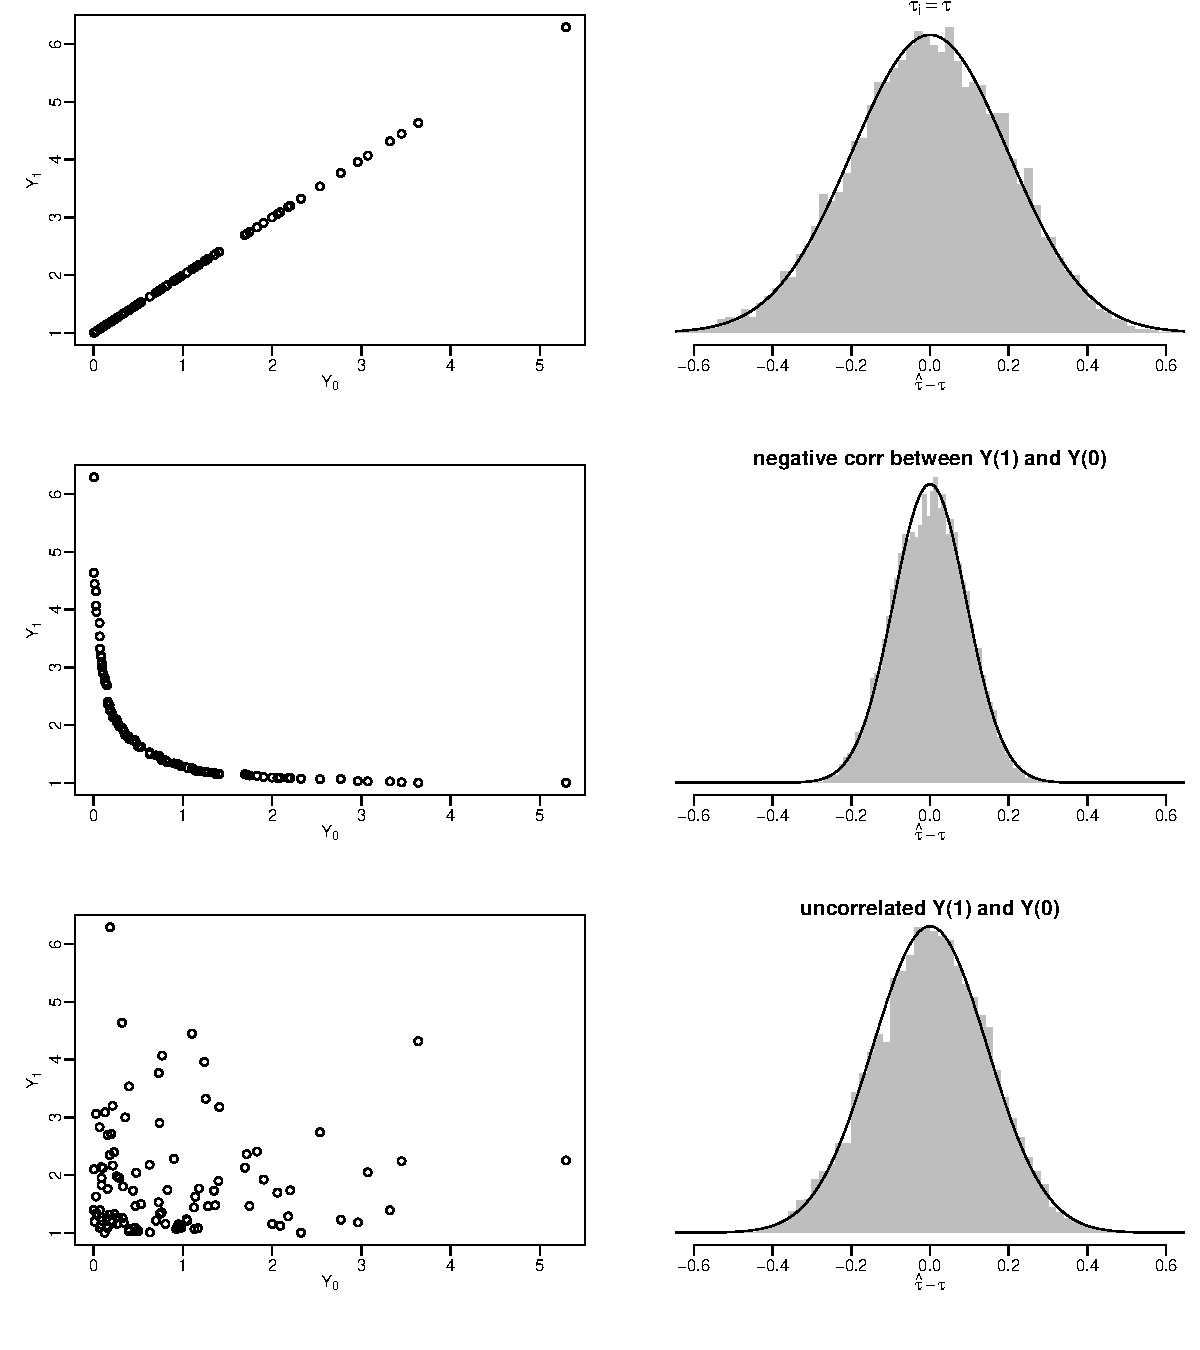
\includegraphics[width = \textwidth]{figures/neymanevaluation3.pdf}
 \caption{左：边际分布相同的潜在结果联合分布。右：不同潜在结果联合分布下，$10^4$次模拟所得$\hat{\tau} - \tau$的抽样分布。}\label{fig::simulation-neyman}
 \end{figure} 
 
 
 
 
 
 \subsection{重尾分布下的正态近似失效}


定理\ref{thm::clt-difference-in-means}中$\hat{\tau}  $的中心极限定理需要正则条件，重尾潜在结果会违反这些条件。可修改前面的模拟说明这一点：保持个体因果效应恒定，但让对照潜在结果以$0.1, 0.3$或$0.5$的概率受到柯西分布成分污染。下面的代码生成污染概率为$0.1$的潜在结果。 

\begin{lstlisting}
eps = rbinom(n, 1, 0.1)
y0 = (1 - eps)*rexp(n) + eps*rcauchy(n)
y1 = y0 + 1
\end{lstlisting} 


图\ref{fig::simulation-neyman-heavytail-1}和\ref{fig::simulation-neyman-heavytail-2}给出了两次实现中$\hat{\tau} - \tau$的直方图及对应正态近似。潜在结果呈重尾时，正态近似很差；而且与图\ref{fig::simulation-neyman}不同，直方图对模拟的随机种子很敏感。 


 \begin{figure}
 \centering 
 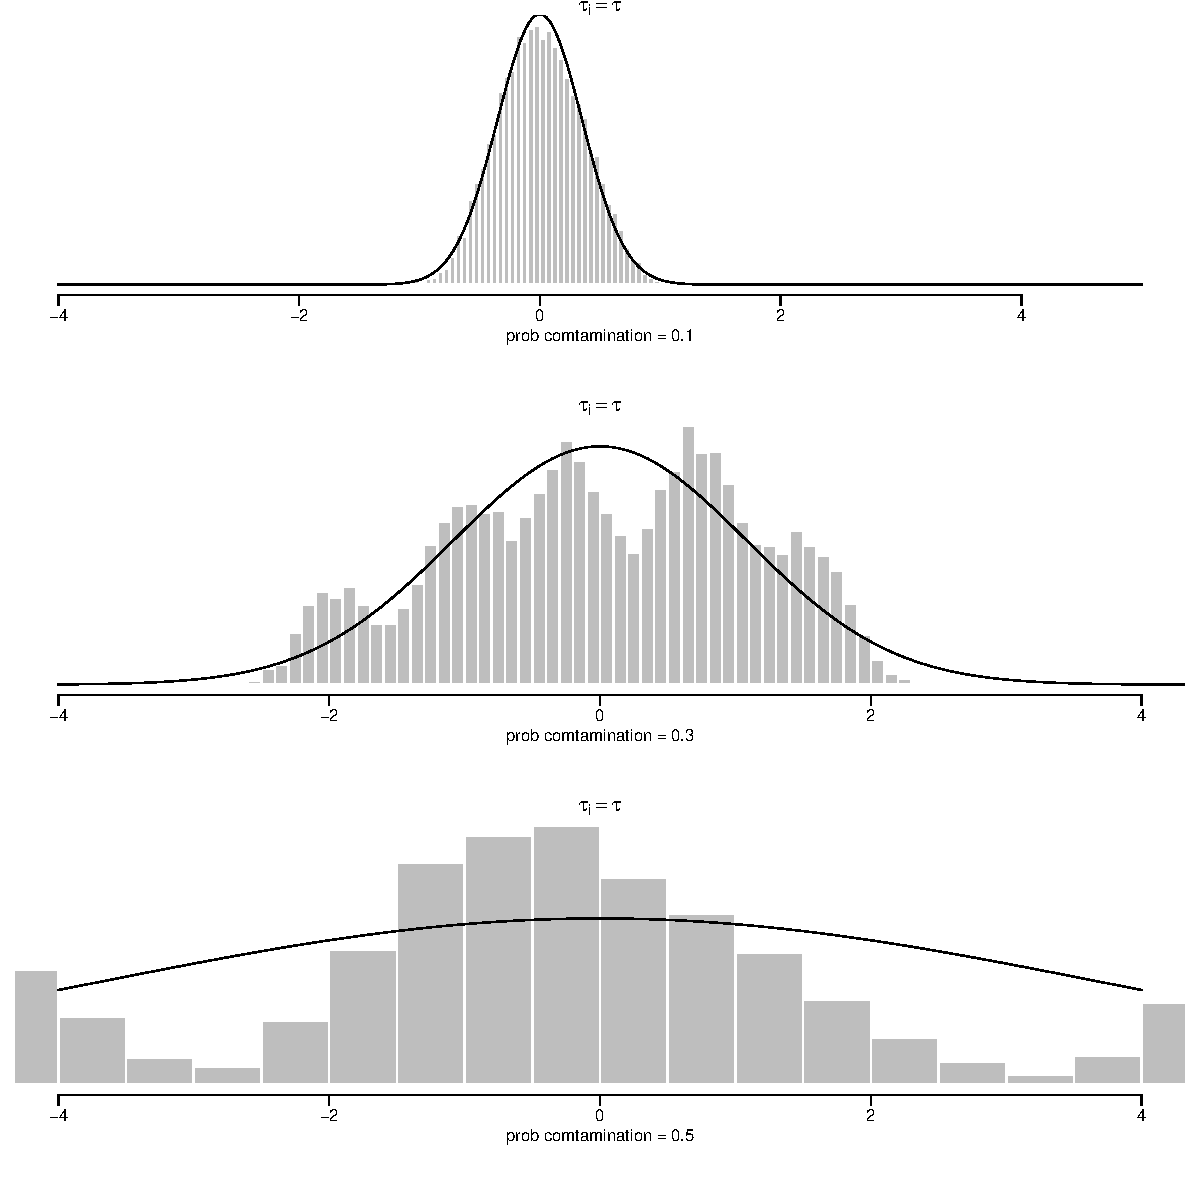
\includegraphics[width = \textwidth]{figures/neyman_comtamination_realized1.pdf}
 \caption{潜在结果受到不同概率污染时$\hat{\tau} - \tau$的抽样分布：第一次实现}\label{fig::simulation-neyman-heavytail-1}
 \end{figure} 
 
  \begin{figure}
 \centering 
 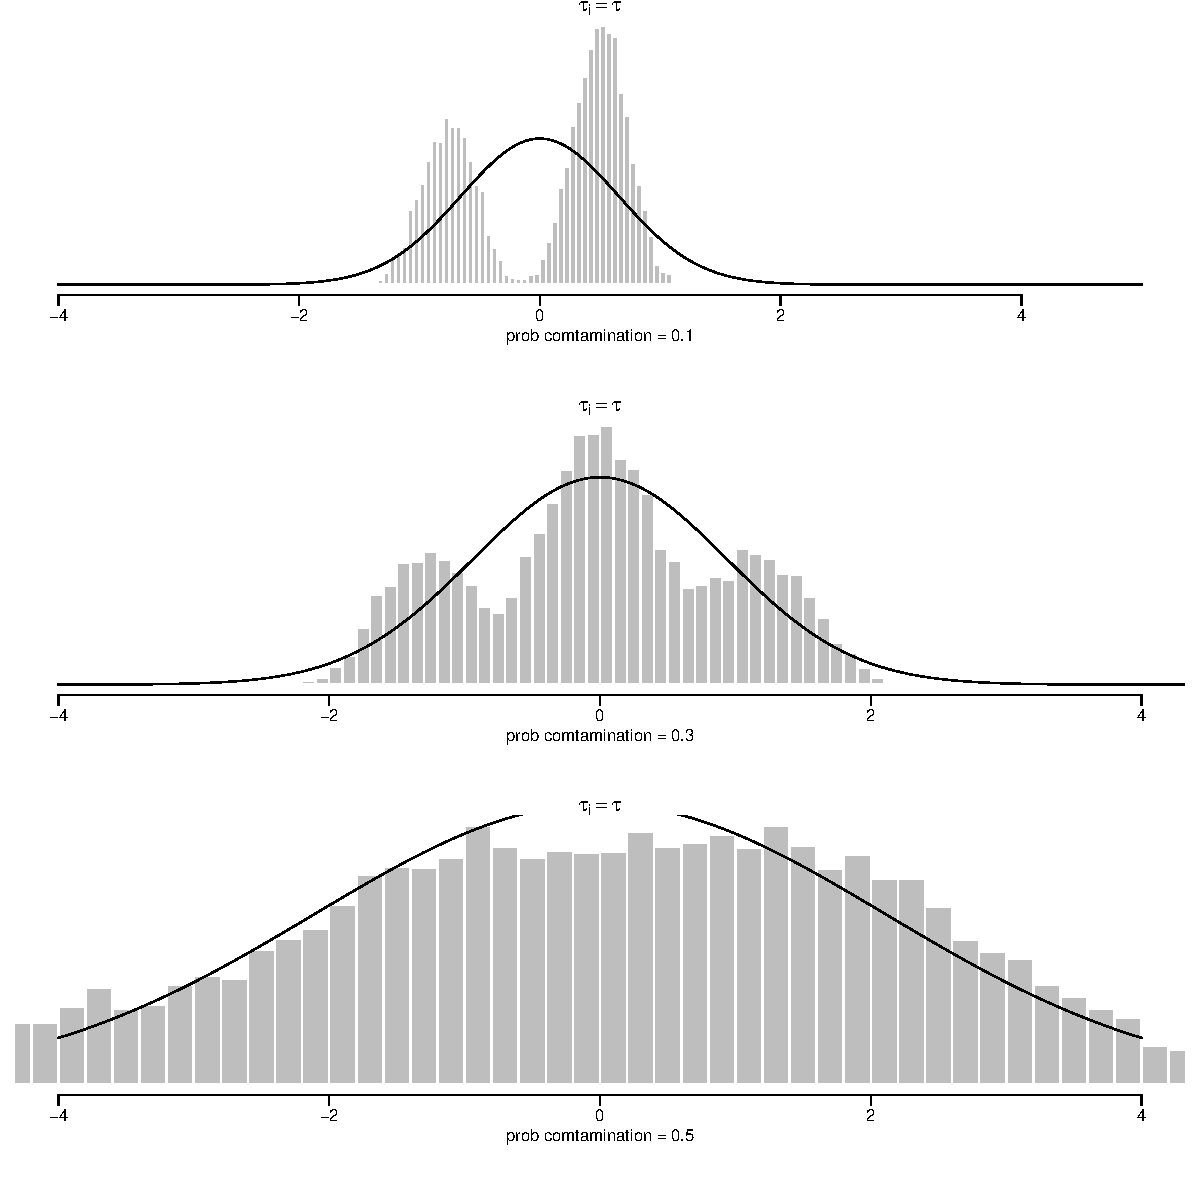
\includegraphics[width = \textwidth]{figures/neyman_comtamination_realized2.pdf}
 \caption{潜在结果受到不同概率污染时$\hat{\tau} - \tau$的抽样分布：第二次实现}\label{fig::simulation-neyman-heavytail-2}
 \end{figure} 
 
 


\subsection{实际数据应用}
\label{sec::example-neyman-formula}


第\ref{sec::frt-lalonde-experiment}节用\ri{lalonde}数据说明了 FRT，现在用同一数据说明本章理论。 
\begin{lstlisting}
> library(Matching)
> data(lalonde)
> z = lalonde$treat
> y = lalonde$re78
\end{lstlisting} 

利用定理\ref{thm::neyman1923}的公式，容易计算点估计与标准误：
\begin{lstlisting}
> n1= sum(z)
> n0= length(z) - n1
> tauhat = mean(y[z==1]) - mean(y[z==0])
> vhat   = var(y[z==1])/n1 + var(y[z==0])/n0
> sehat  = sqrt(vhat)
> tauhat
[1] 1794.343
> sehat
[1] 670.9967
\end{lstlisting} 

此结果与OLS所得估计量高度吻合。而使用EHW稳健标准误修正后所得置信区间则与内曼理论预期完全一致。 
\begin{lstlisting}
> olsfit = lm(y ~ z)
> summary(olsfit)$coef[2, 1: 2]
  Estimate Std. Error 
 1794.3431   632.8536 
 \end{lstlisting} 
但上述标准误比定理\ref{thm::neyman1923}给出的标准误小得多，可以通过 EHW 稳健标准误解决。 
\begin{lstlisting}
> library(car)
> sqrt(hccm(olsfit)[2, 2])
[1] 672.6823
> sqrt(hccm(olsfit, type = "hc0")[2, 2])
[1] 669.3155
> sqrt(hccm(olsfit, type = "hc2")[2, 2])
[1] 670.9967
 \end{lstlisting} 





\section{作业习题}

\paragraph{引理\ref{lemma::variancecovariancetau}的证明}\label{hw::proof-covariance-basic}


证明引理 \ref{lemma::variancecovariancetau}。 


\paragraph{定理\ref{thm::neyman1923}的另类证明}\label{hw::neyman-alternative-proof}


在完全随机实验下，计算
$$
\var\{  \hat{\bar{Y}}(1)  \} ,\quad
\var\{  \hat{\bar{Y}}(0)  \} ,\quad
\cov\{  \hat{\bar{Y}}(1) ,  \hat{\bar{Y}}(0)  \} 
$$
并据此计算$\var(\hat{\tau} )$。 

注：使用第\ref{chapter::SRS-appendix}章的结论。 





\paragraph{内曼推断与OLS}
\label{hw::neyman-ols-nox}


证明\eqref{eq::ols-difference-in-means}至\eqref{eq::ols-ehw}。此外，证明 EHW 稳健方差估计的 HC2 变体恰好恢复$\hat{V}$。 

注：第\ref{appendix::basic-linear-regression}章回顾了 OLS 的若干重要技术结论。
 
 



\paragraph{处理效应的异质性影响}\label{hw::treatment-effect-heterogeneity-neyman}


证明$S^2(\tau) = 0$蕴含$S^2(1) = S^2(0)$，并举出满足$S^2(1) = S^2(0)$但$S^2(\tau) \neq  0$的反例。 


证明$S^2(1) < S^2(0)$蕴含
$$
S(Y(0),\tau)  = (n-1)^{-1} \sumn \{ Y_i(0)  - \bar{Y}(0) \} (\tau_i - \tau) <0.
$$
并举出满足$S^2(1) > S^2(0)$但$S(Y(0),\tau)  < 0 .$的反例。



注：第一条说明，没有处理效应异质性就意味着处理与对照潜在结果的方差相等，但逆命题不成立。第二条说明，若处理潜在结果的方差小于对照潜在结果的方差，则个体处理效应与对照潜在结果负相关，逆命题同样不成立。相关讨论见\citet[][page 293]{gerber2012field}和\citet[][Appendix B.3]{ding2019decomposing}。 



\paragraph{方差估计式的优化}
\label{hw::better-bound-neyman}


\cite{Neyman:1923}的保守方差估计本质上采用了真实方差的上界
$$
\var(\widehat{\tau}) = \frac{S^2(1)}{n_1} + \frac{S^2(0)}{n_0} - \frac{S^2(\tau)}{n} \leq \frac{S^2(1)}{n_1} + \frac{S^2(0)}{n_0},
$$
这里使用了显然成立的$S^2(\tau) \geq 0$。证明另一个上界
\begin{eqnarray}\label{hw::cs-bound-neyman}
\var(\widehat{\tau})  \leq   \frac{1}{n} \left\{   \sqrt{  \frac{n_0}{n_1}  } S(1) +  \sqrt{  \frac{n_1}{n_0}  } S(0)   \right\}^2.
\end{eqnarray}
并说明\eqref{hw::cs-bound-neyman}何时取等号。 

根据上界\eqref{hw::cs-bound-neyman}，可构造另一个保守方差估计量
$$
\hat{V}' =  \frac{1}{n} \left\{   \sqrt{  \frac{n_0}{n_1}  } \hat S(1) +  \sqrt{  \frac{n_1}{n_0}  } \hat S(0)   \right\}^2.
$$
第\ref{sec::simulation-neyman-formula}节的模拟使用了$\hat{V}$。请重复模拟，加入方差估计量$\hat{V}' $及相应置信区间进行比较。 



注：证明时可参考第\ref{sec::cauchy-schwarz-inequality}节。上界\eqref{hw::cs-bound-neyman}还能改进；\citet{aronow2014sharp}利用 Fréchet--Hoeffding 不等式推导了$\var(\widehat{\tau}) $的尖锐上界。这些改进在实践中很少使用，主要有两个原因：一是比可方便地用 OLS 实现的$\hat{V}$复杂；二是基于$\hat{V}$的置信区间也适用于其他表述，例如结果对处理的真实线性模型，而这些改进一般不具备这种性质。因此，尽管理论上有趣，实际影响较小。 
 


\paragraph{\citet{Neyman:1923}定理的向量化拓展} \label{hw::vector-neyman1923}

\citet{Neyman:1923}的经典结论针对标量结果，实践中却常有多个结果。因此，将潜在结果推广为向量，考虑向量结果$\bm{V}  \in \mathbb{R}^K$上的平均因果效应：
$$
\tau_{\bm{V}} = \frac{1}{n}  \sumn \left\{  \bm{V}_i(1) - \bm{V}_i(0) \right\},
$$
其中$\bm{V}_i(1)$和$\bm{V}_i(0)$是单位$i$的$\bm{V}$潜在结果。$\tau_{\bm{V}}$的 Neyman 型估计量为处理组与对照组观测结果样本均值向量之差：
$$
\widehat{ \tau}_{\bm{V}} = \bar{\bm{V}}_1  - \bar{\bm{V}}_0 
= \frac{1}{n_1}   \sumn Z_i  \bm{V}_i   - \frac{1}{n_0}  \sumn (1-Z_i) \bm{V}_i . 
$$


考虑完全随机实验。证明$\widehat{ \tau}_{\bm{V}} $是$\tau_{\bm{V}} $的无偏估计，求$\widehat{ \tau}_{\bm{V}} $的协方差矩阵，并构造一个可能保守的方差估计量。 


\paragraph{完全随机实验下的统计推断}\label{hw::bre-inference}


探讨FRT在随机分配机制下的适用性，比较不同估计量及其渐近特性。 

\begin{definition}
[BRE]\label{def::BRE}
各处理指标$Z_i$独立同分布于 Bernoulli$(\pi)$，处理组人数为$n_1 = \sumn Z_i$，对照组人数为$n_0 = \sumn (1-Z_i)$。 
\end{definition}



首先，可以用 FRT 分析伯努利随机实验（BRE）。如何在 BRE 中检验$\HF$？若实际设计为 BRE，能否使用与完全随机实验相同的 FRT 程序？可以则说明依据，不可以则解释原因。

其次，可像\citet{Neyman:1923}分析完全随机实验那样，构造$\tau$的点估计及对应方差估计。 
\begin{enumerate}
\item
$\hat{\tau}$是$\tau$的无偏估计吗？是否一致？
\item
构造$\tau$的无偏估计量。
\item
比较上述无偏估计量的方差与$\hat{\tau}$的渐近方差。 
\end{enumerate}

注：在 BRE 下，估计量$\hat{\tau}$没有有限方差，但其渐近分布的方差有限。 



\paragraph{推荐阅读}

 \citet{Ding:2014}比较了分析完全随机实验的 Fisher 方法和 Neyman 方法。 




\chapter{随机实验中的分层与后分层}
 \chaptermark{分层与后分层}
\label{chapter::stratification-poststratification}

\begin{quotation}
能分层的就分层，不能分层的就随机化。  

--- \citet[][page 103]{box1978statistics}
\end{quotation}

这是 George Box 第二著名的名言。\footnote{他最著名的名言是“所有模型都是错的，但有些是有用的”\citep[][page 202]{box1979robustness}。}本章将解释它的含义。



\section{分层}



完全随机实验可能偶然产生不理想的处理分配。先考虑离散协变量$X_i   \in \{ 1, \ldots, K \}$，定义$n_{[k]} = \#\{ i: X_i    =k  \}$和$\pi_{[k]} = n_{[k]} / n$为第$k$层的单位数及其比例，$(k=1, \ldots, K)$。完全随机实验将$n_1$个单位分到处理组、$n_0$个单位分到对照组，使第$k$层内的处理和对照单位数分别为
$$
n_{[k]1} = \#\{ i: X_i   = k, Z_i = 1 \},\quad
n_{[k]0} = \#\{ i: X_i   = k, Z_i = 0 \}
$$
对于某些$k$，$n_{[k]1}$或$n_{[k]0}$有正概率为零，即某些层可能只有处理单位或只有对照单位。即使各$n_{[k]1}$和$n_{[k]0}$都不为零，也很可能有
\begin{equation}
\frac{  n_{[k]1} }{n_1}  -  \frac{  n_{[k]0} }{n_0} \neq 0 ,
\label{eq::covarianceimbK}
\end{equation}
且差异可能很大。因此，第$k$层的单位在处理组与对照组中的比例不同，尽管其差的期望为零（见习题\ref{hw::balance-discrete-CRE}）：
\begin{equation}\label{eq::balance-discrete-CRE}
E\left(  \frac{  n_{[k]1} }{n_1}  -  \frac{  n_{[k]0} }{n_0} \right) = 0.
\end{equation}
若某些层$k$中的$n_{[k]1}  / n_1  -  n_{[k]0} / n_0$很大，两组就存在不理想的协变量不平衡。这会降低实验质量，使结果难以解释，因为结果差异可能来自处理，也可能来自协变量不平衡。 



如何避免这种失衡？此时可采用分层随机实验法。

\begin{definition}[SRE]
\label{def::SRE}
固定各$n_{[k]1}$或各$n_{[k]0}$，在离散协变量$X$的$K$个层内分别实施$K$个相互独立的完全随机实验。
\end{definition}

在农业实验中，分层随机实验也称{\it 随机区组设计}，各层称为区组。相应地，{\it 分层随机化}也称{\it 区组随机化}。\footnote{第\ref{sec::fisherian-principles-experiments}节介绍了 Fisher 实验设计的两个原则：{\it 随机化}与{\it 重复}；{\it 区组化}是第三个原则。}分层随机实验的随机分配总数为
$$
\prod_{k=1}^K  \binom{  n_{[k]} }{  n_{[k]1} } ,
$$
每个可行分配等概率出现。第$k$层接受处理的比例为
$$
e_{[k]} = \frac{n_{[k]1}}{n_{[k]}},
$$
这也称{\it 倾向得分}，将在本书第\ref{part::observational-studies}部分发挥核心作用（见定义\ref{def::pscore}）。分层随机实验不同于完全随机实验：第一，前者的所有可行分配只是后者可行分配的子集，因此
$$
\prod_{k=1}^K  \binom{  n_{[k]} }{  n_{[k]1} } < 
\binom{n}{n_1} ;
$$
第二，$e_{[k]} $在分层随机实验中固定，在完全随机实验中随机。  


每个单位$i$有潜在结果$Y_i(1)$、$Y_i(0)$，个体因果效应为$\tau_i = Y_i(1) - Y_i(0) . $。第$k$层的平均因果效应为
$$
\tau_{[k]} = n_{[k]}^{-1} \sum_{X_i   = k} \tau_i .
$$
总体平均因果效应为
$$
\tau = n^{-1} \sumn \tau_i = n^{-1} \sum_{k=1}^K \sum_{X_i   = k} \tau_i =  \sum_{k=1}^K  \pi_{[k]}  \tau_{[k]},
$$
即各层平均因果效应的加权平均。 


若关注$\tau_{[k]} $，可在第$k$层内使用第\ref{ch::frt-cre}、\ref{chapter::neyman-cr}章完全随机实验的方法。下面讨论对$\tau$的统计推断。 


\section{FRT}
\label{sec::sre-frt}


\subsection{理论}与完全随机实验的讨论相对应，先介绍分层随机实验中的 FRT。尖锐零假设仍为
$$
\HF: Y_i(1) = Y_i(0) \text{ for all units } i=1, \ldots, n.
$$
FRT 的基本思想适用于任意随机实验：可以使用任意统计量$T = T(\bm{Z}, \bm{Y}, \bm{X})$，其中$\bm{Z}, \bm{Y}$与$\bm{X}$依次表示处理向量、观测结果向量与协变量矩阵。在分层随机实验及$\HF$下，$\bm{Z}$的分布已知，故$T$的分布也已知。但必须注意两点：第一，模拟处理向量时，必须按定义\ref{def::SRE}在$X$的各层内置换处理指标。所得检验有时称为{\it 条件随机化检验}或{\it 条件置换检验}。第二，应选择能体现分层随机实验特点的统计量。下面给出若干常用选择。

\begin{example}[分层差异估计量]
\label{eg::stratifiedestimator}
为估计$\tau$（见后文第\ref{sec::sre-neyman}节），可在 FRT 中使用分层估计量
$$
\hat{\tau}_\textsc{S} = \sum_{k=1}^K  \pi_{[k]} \hat{\tau}_{[k]},
$$
其中
$$
\hat{\tau}_{[k]} = n_{[k]1}^{-1} \sumn I(X_i  =k, Z_i=1) Y_i - n_{[k]0}^{-1} \sumn I(X_i  =k, Z_i=0) Y_i 
$$
是第$k$层内的均值差。 
\end{example}




\begin{example}[标准化分层估计量]
\label{eg::student-stratifiedestimator}
受双样本问题的学生化统计量启发，可定义如下标准化统计量：
$$
t_\textsc{S} = 
\frac{ \hat{\tau}_\textsc{S}  }{  \sqrt{\hat{V}_\textsc{S}  }},
$$
其中
$$
\hat{V}_\textsc{S} = \sum_{k=1}^K  \pi_{[k]}^2 \left(  \frac{\hat{S}_{[k]}^2(1)}{ n_{[k]1} } +  \frac{ \hat{S}_{[k]}^2(0)}{ n_{[k]0} } \right)
$$
$\hat{S}_{[k]}^2(1)$ 与 $\hat{S}_{[k]}^2(0)$ 分别为该层处理组与对照组的样本方差。该统计量设计思路源自下文 \ref{sec::sre-neyman} 所述的内曼视角。
\end{example}




\begin{example}[威尔科克森秩和合并法]
\label{eg::vanelteren}
先在第$k$层内计算 Wilcoxon 秩和统计量$W_{[k]}$（回顾例\ref{example::wilcoxon-cre}），再合成为
$$
W_\textsc{S} = \sum_{k=1}^K   c_{[k]}  W_{[k]}   . 
$$
根据不同渐近设定与最优性准则，\citet{van1960combination}提出两种权重：
$$
c_{[k]}  = \frac{1}{  n_{[k]1}  n_{[k]0} },
$$
以及
$$ 
c_{[k]}  = \frac{1}{  n_{[k]}  +1 } .
$$
这些权重的理论依据涉及较多技术细节，其他权重选择也可能合理。 
\end{example}


 


\begin{example}[\citet{hodges1962rank} 的对齐秩和检验]
\label{eg::hodgeslehmann}
\citet{van1960combination}的统计量适合层数较少、每层较大的情形；层数多而每层很小时，它进行的比较不够充分，可能损失信息。\citet{hodges1962rank}提出将结果标准化后，作更多跨层比较。具体做法是先按层均值中心化结果：
$$
\tilde{Y}_i = Y_i  - \bar{Y}_{[k]}
$$
其中，若$X_i = k$，层均值为$
\bar{Y}_{[k]} = n_{[k]}^{-1} \sum_{X_i   = k} Y_i
$；然后对合并后的结果$(\tilde{Y}_1, \ldots, \tilde{Y}_n)$计算秩$(\tilde{R}_1, \ldots, \tilde{R}_n)$，最后构造统计量
$$
\tilde{W} = \sumn Z_i \tilde{R}_i.
$$
\end{example}


基于上述统计量，我们可模拟其在分层实验下的经验分布，计算均值、方差及 $p$ 值。目前尚未见针对分层实验的柯尔莫哥洛夫-斯米尔诺夫统计量研究，下文将作初步探讨。 


查阅一番后，我未找到详细讨论分层随机实验中 Kolmogorov--Smirnov 统计量的文献。下面给出我的建议。


 \begin{example}[Kolmogorov--Smirnov 统计量]
\label{eg::ks-stratified}
在第$k$层内计算处理组与对照组结果经验分布的最大差$D_{[k]}$。最终统计量可以取
$$
D_\textsc{S}  = \sum_{k=1}^K    c_{[k]}    D_{[k]}
$$
或
$$
D_{\max} = \max_{1\leq k \leq K}  c_{[k]}   D_{[k]},
$$
权重$ c_{[k]}   = \sqrt{   n_{[k]1}  n_{[k]0} /  n_{[k]}  }$的依据，是$n_{[k]1} $和$ n_{[k]0} $趋于无穷时$D_{[k]}$的极限分布（见例\ref{eg::ks-CRE}）。$D_\textsc{S} $与$D_{\max} $更适合所有层样本量都较大的情形。另一个合理选择为
$$
D =  \max_y \Big |  \sum_{k=1}^K  \pi_{[k]}  \{  \hat{F}_{[k]1}(y)  - \hat{F}_{[k]0}(y) \}   \Big | ,
$$
其中$\hat{F}_{[k]1}(y)  $和$ \hat{F}_{[k]0}(y)$分别是各层处理组与对照组结果的经验分布函数。统计量$D$既适用于大层，也适用于许多小层。 
\end{example}
 
 
 
 \subsection{实例应用}
 \label{sec::frt-pennbonus}
 
 
 
宾州奖金实验可用来说明分层随机实验的 FRT。\citet{koenker2002inference}使用的数据来自按\ri{quarter}分层的职业培训项目，结果为就业前的等待时长。 

\begin{lstlisting}
> penndata = read.table("Penn46_ascii.txt")
> z = penndata$treatment
> y = log(penndata$duration)
> block = penndata$quarter
> table(penndata$treatment, penndata$quarter)
   
      0   1   2   3   4   5
  0 234  41 687 794 738 860
  1  87  48 757 866 811 461
\end{lstlisting} 


下面只考虑$\hat{\tau}_\textsc{S}$和$W_\textsc{S}$，其他统计量的 FRT 留作习题\ref{hw::FRT-SRE-more}。以下函数计算$\hat{\tau}_\textsc{S}$与$W_\textsc{S}$：

\begin{lstlisting}
stat_SRE = function(z, y, x)
{
       xlevels = unique(x)
       K       = length(xlevels)
       PiK     = rep(0, K)
       TauK    = rep(0, K)
       WK      = rep(0, K)
       for(k in 1:K)
       {
             xk         = xlevels[k]
             zk         = z[x == xk]
             yk         = y[x == xk]
             PiK[k]     = length(zk)/length(z)
             TauK[k]    = mean(yk[zk==1]) - mean(yk[zk==0])
             WK[k]      = wilcox.test(yk[zk==1], yk[zk==0])$statistic
       }
       
       return(c(sum(PiK*TauK), sum(WK/PiK)))
}
\end{lstlisting} 


下面的函数根据观测数据，生成分层随机实验的一次随机处理分配：

\begin{lstlisting}
zRandomSRE = function(z, x)
{
         xlevels = unique(x)
         K       = length(xlevels)
         zrandom = z
         for(k in 1:K)
         {
              xk = xlevels[k]   
              zrandom[x == xk] = sample(z[x == xk])
         }
         
         return(zrandom)
}
\end{lstlisting} 


利用上述数据和函数，可模拟检验统计量的随机化分布并计算$p$值。 
\begin{lstlisting}
> stat.obs = stat_SRE(z, y, block)
> MC = 10^3
> statSREMC = matrix(0, MC, 2)
> for(mc in 1:MC)
+ {
+     zrandom         = zRandomSRE(z, block) 
+     statSREMC[mc, ] = stat_SRE(zrandom, y, block)     
+ }
> mean(statSREMC[, 1] <= stat.obs[1])
[1] 0.002
> mean(statSREMC[, 2] <= stat.obs[2])
[1] 0.001
\end{lstlisting} 
由于处理对结果产生负向效应，这里根据左尾概率计算$p$值。观测统计量和随机化分布的更多细节见图\ref{fig::frt_sre_penn}。  
 

 
\begin{figure}
\centering
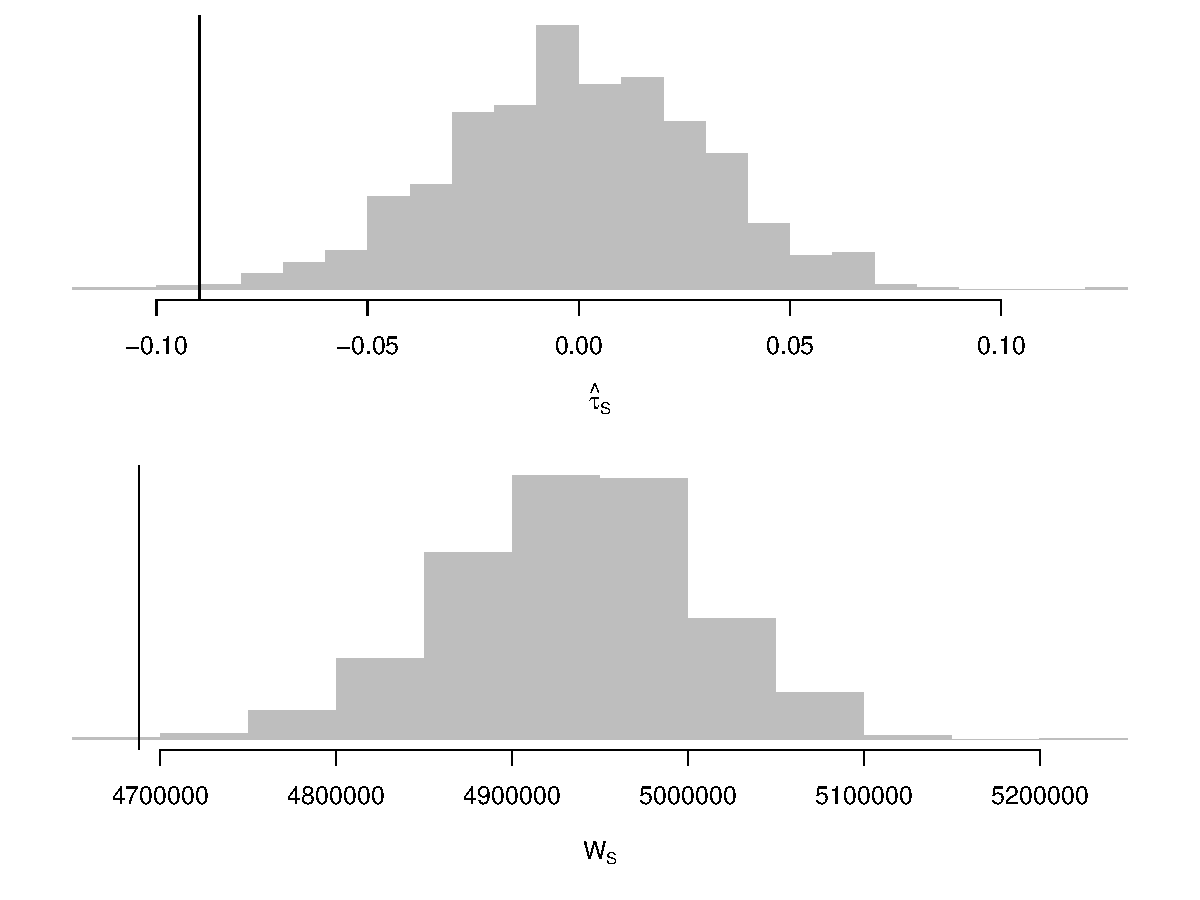
\includegraphics[width = \textwidth]{figures/FRT_SRE_histograms.pdf}
\caption{宾州奖金实验中$\hat{\tau}_\textsc{S}$与$W_\textsc{S}$的随机化分布，使用$10^4$次蒙特卡洛抽样}\label{fig::frt_sre_penn}
\end{figure} 



\section{内曼推断法}
\label{sec::sre-neyman}
\subsection{点估计与区间估计}

分层随机实验本质上由$K$个独立的完全随机实验组成，据此可推广\citet{Neyman:1923}的结论。第$k$层内，均值差$\hat{\tau}_{[k]}$是$\tau_{[k]}$的无偏估计，方差为
$$
\var ( \hat{\tau}_{[k]}) =  \frac{S_{[k]}^2(1)}{ n_{[k]1} } +  \frac{S_{[k]}^2(0)}{ n_{[k]0} }
- \frac{  S_{[k]}^2(\tau) }{ n_{[k]} },
$$
其中$ S_{[k]}^2(1), S_{[k]}^2(0)$与$S_{[k]}^2(\tau)$分别为层内潜在结果和个体因果效应的方差。因此，分层估计量$\hat{\tau}_\textsc{S} = \sum_{k=1}^K  \pi_{[k]} \hat{\tau}_{[k]}$是$\tau =\sum_{k=1}^K  \pi_{[k]}  \tau_{[k]} $的无偏估计，方差为
$$
\var( \hat{\tau}_\textsc{S}   ) = \sum_{k=1}^K  \pi_{[k]}^2   \var ( \hat{\tau}_{[k]}).
$$
若$n_{[k]1} \geq 2$且$n_{[k]0} \geq 2$，可计算第$k$层内结果的样本方差$\hat{S}_{[k]}^2(1)$与$\hat{S}_{[k]}^2(0)$，并构造保守方差估计量
$$
\hat{V}_\textsc{S}  = \sum_{k=1}^K  \pi_{[k]}^2 \left(  \frac{\hat{S}_{[k]}^2(1)}{ n_{[k]1} } +  \frac{ \hat{S}_{[k]}^2(0)}{ n_{[k]0} } \right), 
$$
其中$\hat{S}_{[k]}^2(1)$和$\hat{S}_{[k]}^2(0)$分别为各层处理组与对照组结果的样本方差。对$\hat{\tau}_\textsc{S} $作正态近似，可构造$\tau$的 Wald 型$1-\alpha$置信区间：
$$
\hat{\tau}_\textsc{S} \pm z_{1-\alpha/2} \sqrt{  \hat{V}_\textsc{S}  } . 
$$
从检验角度，在$\HN: \tau=0$下，可将$t_\textsc{S} =   \hat{\tau}_\textsc{S} / \sqrt{  \hat{V}_\textsc{S}  }$与标准正态分位点比较，得到渐近$p$值。统计量$t_\textsc{S} $也出现在例\ref{eg::student-stratifiedestimator}的 FRT 中。后文第\ref{chapter::unification-fisher-neyman}章将证明，以$t_\textsc{S} $进行 FRT，在$\HF$下给出有限样本精确$p$值，在$\HN$下给出渐近有效$p$值。 



这里略去$\hat{\tau}_\textsc{S} $中心极限定理的技术细节。\citet{liu2020regression}给出了证明，同时覆盖少数大层与许多小层两种渐近情形。后文第\ref{sec::sre-neyman-example}节通过数值例子说明这一理论问题。 


\subsection{数值示例}
\label{sec::sre-neyman-example}

下面的函数计算分层随机实验的 Neyman 点估计和方差估计：
\begin{lstlisting}
Neyman_SRE = function(z, y, x)
{
       xlevels = unique(x)
       K       = length(xlevels)
       PiK     = rep(0, K)
       TauK    = rep(0, K)
       varK    = rep(0, K)
       for(k in 1:K)
       {
             xk         = xlevels[k]
             zk         = z[x == xk]
             yk         = y[x == xk]
             PiK[k]     = length(zk)/length(z)
             TauK[k]    = mean(yk[zk==1]) - mean(yk[zk==0])
             varK[k]    = var(yk[zk==1])/sum(zk) + 
                               var(yk[zk==0])/sum(1 - zk)
       }
       
       return(c(sum(PiK*TauK), sum(PiK^2*varK)))
}
\end{lstlisting} 


第一个模拟设定取$K=5$，每层$80$个单位。\ri{TauHat}和\ri{VarHat}分别保存$10^4$次模拟的点估计与方差估计。 
\begin{lstlisting}
> K  = 5
> n  = 80
> n1 = 50
> n0 = 30
> x  = rep(1:K, each = n)
> y0 = rexp(n*K, rate = x)
> y1 = y0 + 1
> zb = c(rep(1, n1), rep(0, n0))
> MC = 10^4
> TauHat = rep(0, MC)
> VarHat = rep(0, MC)
> for(mc in 1:MC)
+ {
+   z  = replicate(K, sample(zb))
+   z  = as.vector(z)
+   y  = z*y1 + (1-z)*y0
+   est = Neyman_SRE(z, y, x) 
+   TauHat[mc] = est[1]
+   VarHat[mc] = est[2]
+ }
> var(TauHat)
[1] 0.002248925
> mean(VarHat)
[1] 0.002266396
\end{lstlisting} 
图\ref{fig::2CLTs}上图给出点估计量的直方图，它围绕真实参数对称，呈钟形。由于个体因果效应恒定，方差估计量的平均值几乎等于点估计量的真实方差。 



第二个模拟设定取$K=50$，每层$8$个单位。 
\begin{lstlisting}
> K  = 50
> n  = 8
> n1 = 5
> n0 = 3
> x  = rep(1:K, each = n)
> y0 = rexp(n*K, rate = log(x + 1))
> y1 = y0 + 1
> zb = c(rep(1, n1), rep(0, n0))
> MC = 10^4
> TauHat = rep(0, MC)
> VarHat = rep(0, MC)
> for(mc in 1:MC)
+ {
+   z  = replicate(K, sample(zb))
+   z  = as.vector(z)
+   y  = z*y1 + (1-z)*y0
+   est = Neyman_SRE(z, y, x) 
+   TauHat[mc] = est[1]
+   VarHat[mc] = est[2]
+ }
> 
> hist(TauHat, xlab = expression(hat(tau)[S]),
+      ylab = "", main = "many small strata", 
+      border = FALSE, col = "grey",
+      breaks = 30, yaxt = 'n',
+      xlim = c(0.8, 1.2))
> abline(v = 1)
> 
> var(TauHat)
[1] 0.001443111
> mean(VarHat)
[1] 0.001473616
\end{lstlisting} 
图\ref{fig::2CLTs}下图给出点估计量的直方图，它同样围绕真实参数对称，呈钟形。由于个体因果效应恒定，方差估计的平均值再次几乎等于点估计量的真实方差。 

\begin{figure}
\centering
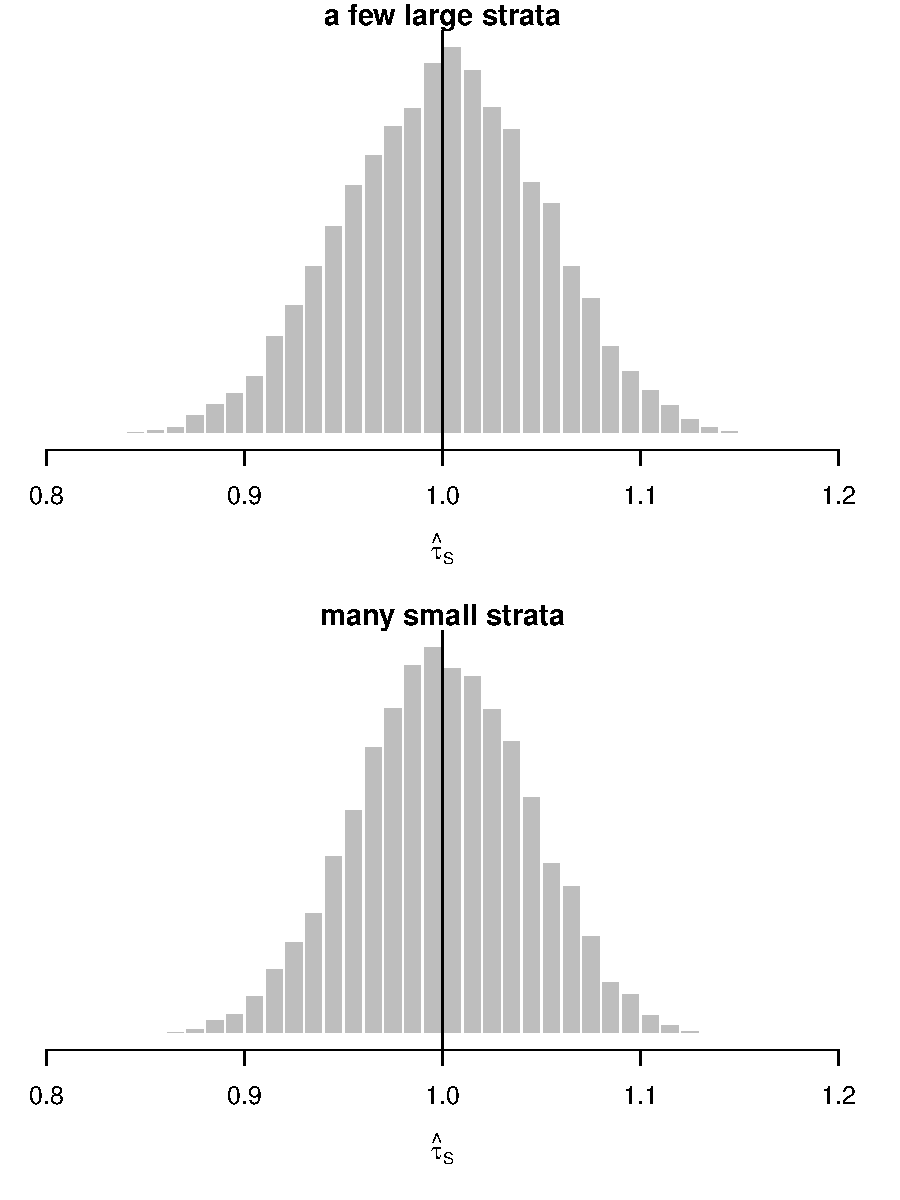
\includegraphics[width = \textwidth]{figures/SRE_CLT_2Regimes.pdf}
\caption{两种分层规模的渐近正态性表现}\label{fig::2CLTs}
\end{figure} 




最后以宾州奖金实验说明分层随机实验的 Neyman 推断。对数据使用\ri{Neyman_SRE}函数，得到：
\begin{lstlisting}
> penndata = read.table("Penn46_ascii.txt")
> z = penndata$treatment
> y = log(penndata$duration)
> block = penndata$quarter
> est = Neyman_SRE(z, y, block)
> est[1]
[1] -0.08990646
> sqrt(est[2])
[1] 0.03079775
\end{lstlisting} 
因此，该职业培训项目显著缩短了就业前等待时长的对数。 


\subsection{比较分层随机实验与完全随机实验}

分层随机实验相比完全随机实验有什么好处？前面从协变量平衡出发引入分层设计，下面说明更好的平衡还能提高平均因果效应的估计精度。为公平比较，假定对所有$k$都有$e_{[k]} = e$，此时均值差等于分层估计量：
\begin{equation}
\label{eq::dim=stratified}
\hat{\tau} = \hat{\tau}_\textsc{S}.
\end{equation}
\eqref{eq::dim=stratified}的证明留作习题\ref{hw::sre-additional-neyman}。 




下面比较抽样方差。经典方差分析将总方差分解为层内方差与层间方差，得到
\begin{eqnarray*}
S^2(1) &=&  (n-1)^{-1} \sumn \{  Y_i(1) - \bar{Y}(1) \}^2 \\
&=& (n-1)^{-1} \sum_{k=1}^K \sum_{X_i   = k} \{ Y_i(1) - \bar{Y}_{[k]}(1)  + \bar{Y}_{[k]}(1)  -   \bar{Y}(1)  \}^2 \\
&=& (n-1)^{-1} \sum_{k=1}^K \sum_{X_i   = k} \left[  \{ Y_i(1) - \bar{Y}_{[k]}(1) \}^2 +  \{ \bar{Y}_{[k]}(1)  -   \bar{Y}(1)  \}^2 \right] \\
&=& \sum_{k=1}^K \left[   \frac{n_{[k]} - 1}{n-1}   S_{[k]}^2(1)  +  \frac{ n_{[k]}}{ n-1} \{ \bar{Y}_{[k]}(1) - \bar{Y}(1) \}^2  \right],
\end{eqnarray*}
类似地，
\begin{eqnarray*}
S^2(0) &=& \sum_{k=1}^K \left[   \frac{n_{[k]} - 1}{n-1}   S_{[k]}^2(0)  +  \frac{ n_{[k]}}{ n-1} \{ \bar{Y}_{[k]}(0) - \bar{Y}(0) \}^2  \right],\\
S^2(\tau) &=& \sum_{k=1}^K \left[   \frac{n_{[k]} - 1}{n-1}   S_{[k]}^2(\tau)  +  \frac{ n_{[k]}}{ n-1} \{ \tau_{[k]} - \tau \}^2  \right] .
\end{eqnarray*}
完全随机实验下均值差估计量的方差可分解为
\begin{eqnarray*}
&&\var_{\text{CRE}}(  \hat{\tau} )  \\
&=& \frac{S^2(1)}{ n_{1} } +  \frac{S^2(0)}{ n_{0} }
- \frac{  S^2(\tau) }{ n }  \\ 
&=& \sum_{k=1}^K  \left[   \frac{ n_{[k]} - 1}{(n-1)n_1}  S_{[k]}^2(1) + \frac{ n_{[k]} - 1}{ (n-1)n_0}  S_{[k]}^2(0) -  \frac{ n_{[k]} - 1}{(n-1)n}    S_{[k]}^2(\tau) \right] \\
&&  + \sum_{k=1}^K  \left[    \frac{ n_{[k]} - 1}{ (n-1)n_1}  \{ \bar{Y}_{[k]}(1) - \bar{Y}(1) \}^2 +  \frac{ n_{[k]} - 1}{ (n-1)n_0}  \{ \bar{Y}_{[k]}(0) - \bar{Y}(0) \}^2   \right. \\
&& \left.  - \frac{ n_{[k]} - 1  }{ (n-1)n} \{ \tau_{[k]} - \tau \}^2  \right] .
 \end{eqnarray*}
各$n_{[k]}$较大时，近似为
\begin{eqnarray*}
 &&\var_{\text{CRE}}(  \hat{\tau} )  \\
&\approx & 
\sum_{k=1}^K  \left[   \frac{ \pi_{[k]}}{n_1}  S_{[k]}^2(1) + \frac{ \pi_{[k]}}{n_0}  S_{[k]}^2(0) -  \frac{ \pi_{[k]}}{n}    S_{[k]}^2(\tau) \right] \\
&&  + \sum_{k=1}^K  \left[    \frac{ \pi_{[k]}}{n_1}  \{ \bar{Y}_{[k]}(1) - \bar{Y}(1) \}^2 +  \frac{ \pi_{[k]}}{n_0}  \{ \bar{Y}_{[k]}(0) - \bar{Y}(0) \}^2  
 - \frac{ \pi_{[k]}  }{n} \{ \tau_{[k]} - \tau \}^2  \right] .
\end{eqnarray*}
恒定倾向得分假设保证
$$ 
\pi_{[k]} / n_{[k]1}  = 1/(ne), \quad   \pi_{[k]} / n_{[k]0} = 1/\{n(1-e) \},\quad \pi_{[k]} / n_{[k]} = 1/n,
$$
从而可将分层随机实验中$\hat{\tau}_\textsc{S}$的方差改写为
\begin{eqnarray*}
\var_\textsc{SRE}(\hat{\tau}_\textsc{S}) &= & \sum_{k=1}^K  \pi_{[k]}^2 \left[ \frac{S_{[k]}^2(1)}{ n_{[k]1} } +  \frac{S_{[k]}^2(0)}{ n_{[k]0} }
- \frac{  S_{[k]}^2(\tau) }{ n_{[k]} } \right]\\
&=&\sum_{k=1}^K  \left[   \frac{ \pi_{[k]}}{n_1}  S_{[k]}^2(1) + \frac{ \pi_{[k]}}{n_0}  S_{[k]}^2(0) -  \frac{ \pi_{[k]}}{n}    S_{[k]}^2(\tau) \right] .
\end{eqnarray*}
各$n_{[k]}$较大时，$\var_{\text{CRE}}(  \hat{\tau} )$与$\var_\textsc{SRE}(\hat{\tau}_\textsc{S})$之差近似为
$$
\sum_{k=1}^K  \left[    \frac{ \pi_{[k]}}{n_1}  \{ \bar{Y}_{[k]}(1) - \bar{Y}(1) \}^2 +  \frac{ \pi_{[k]}}{n_0}  \{ \bar{Y}_{[k]}(0) - \bar{Y}(0) \}^2  
 - \frac{  \pi_{[k]}  }{n}  ( \tau_{[k]} - \tau  ) ^2  \right] 
 $$
这一差值非负，因为它等于（见习题\ref{hw::compare-CRE-SRE}）
\begin{eqnarray}
\label{eq::difference}
\sum_{k=1}^K\frac{ \pi_{[k]}}{n} 
 \left\{
\sqrt{ \frac{n_0}{n_1} } \{ \bar{Y}_{[k]}(1) - \bar{Y}(1) \} +  \sqrt{ \frac{n_1}{n_0} } \{ \bar{Y}_{[k]}(0) - \bar{Y}(0) \}
 \right\}^2 \geq 0,
\end{eqnarray}
\eqref{eq::difference}仅在对所有$k=1,\ldots, K$均有
$$
\sqrt{ \frac{n_0}{n_1} } \{ \bar{Y}_{[k]}(1) - \bar{Y}(1) \} +  \sqrt{ \frac{n_1}{n_0} } \{ \bar{Y}_{[k]}(0) - \bar{Y}(0) \}
= 0 
$$
的极端情况下为零。若协变量能预测潜在结果，上述各量通常不全为零，因而分层随机实验比完全随机实验更有效率。只有协变量完全没有预测能力的极端情形，大样本效率增益才为零；此时在有限样本中，分层甚至可能降低效率。这呼应了本章开头 George Box 的名言。 

 


最后补充几点。第一，上述比较针对抽样方差，也可比较两种设计下的估计方差，结论类似。第二，增加$K$能提高效率，但论证依赖各层足够大的假设，因此实践中存在权衡。不能任意增大$K$；最极端的情形是$n_{[k]1} = n_{[k]0} = 1$，即第\ref{chapter::mpe}章将介绍的配对实验。 

 




\section{完全随机实验中的后分层}\label{sec::poststra-cre}

在具有离散协变量$X$的完全随机实验中，第$k$层的处理与对照单位数随机；在分层随机实验中，这些数固定。但若给定$\bm{n} = \{  n_{[k]1} , n_{[k]0} \}_{k=1}^K$作条件推断，完全随机实验就变为分层随机实验。从数学上说，若$\bm{n}$的各分量均不为零，则
\begin{equation}\label{eq::condition-to-SRE}
\pr_\textsc{CRE}(\bm{Z} = \bm{z} \mid\bm{n} )
= \frac{ \pr_\textsc{CRE}( \bm{Z} = \bm{z},  \bm{n})   }{ \pr_\textsc{CRE}(   \bm{n})   }
=  \frac{1}{  \prod_{k=1}^K  \binom{  n_{[k]} }{  n_{[k]1} } }  ,
\end{equation}
即完全随机实验中给定$\bm{n}$后$\bm{Z}$的条件分布，与分层随机实验中$\bm{Z}$的分布相同。\eqref{eq::condition-to-SRE}的证明留作习题\ref{hw::CRE-SRE}。因此，给定$\bm{n}$后，可按分层随机实验的方法分析带离散协变量$X$的完全随机实验。具体而言，FRT 变为{\it 条件 FRT}，Neyman 分析变为{\it 后分层}：
$$
\hat{\tau}_\textsc{PS} = \sum_{k=1}^K \pi_{[k]} \hat{\tau}_{[k]},
$$
其形式与$\hat{\tau}_\textsc{S}$相同。给定$\bm{n}$时$\hat{\tau}_\textsc{PS} $的方差，等于分层随机实验下$\hat{\tau}_\textsc{S}$的方差。  


\citet{hennessy2016conditional}通过模拟表明，条件 FRT 的功效往往高于无条件 FRT。\citet{miratrix:2013}从理论上证明，后分层在许多情形下比$\hat{\tau}$更有效率。二者都要求$X$能预测结果。但模拟只覆盖有限的数据生成过程，理论也要求各层足够大。条件 FRT 或后分层不能划分得过细：$K$越大，某些$n_{[k]1} $或$ n_{[k]0}$为零的可能性越高。$n_{[k]1} $或$ n_{[k]0}$很小甚至为零时，FRT 的可行随机分配数大幅减少，功效可能显著降低。Neyman 推断的问题更明显，因为此时甚至无法定义$\hat{\tau}_\textsc{PS}$及其方差估计量。 


分层在设计阶段使用$X$，后分层在分析阶段使用$X$，二者是利用$X$的对偶方法。当各层较大时，两者的差异渐近较小\citep{miratrix:2013}。

\subsection{\citet{meinert1970study}的例子}\label{sec::ps-merinert}

使用\citet{meinert1970study}报告的完全随机实验数据，\citet{rothman2008modern}也曾使用这组数据。处理为甲苯磺丁脲，对照为安慰剂。 
\begin{center} 
\begin{tabular}{ccc}
\multicolumn{3}{c}{ 年龄 $< 55$} \\
\hline 
 & 存活 & 死亡 \\
$Z=1$ &    98 & 8 \\
$Z=0$  & 115 & 5 \\
\hline 
\end{tabular}
%&
\begin{tabular}{ccc}
\multicolumn{3}{c}{ 年龄 $\geq  55$} \\
\hline 
 & 存活 & 死亡 \\
$Z=1$ &    76 & 22 \\
$Z=0$  &  69 & 16 \\
\hline 
\end{tabular}
%&
\begin{tabular}{ccc}
\multicolumn{3}{c}{合计 } \\
\hline 
 & 存活 & 死亡 \\
$Z=1$ &    174 & 30 \\
$Z=0$  & 184 & 21 \\
\hline 
\end{tabular}
\end{center}
 

下表分别给出两层的估计量、后分层估计量、忽略二元协变量的粗估计量，以及各自的标准误。  
\begin{center}
\begin{tabular}{crrrr}
\hline 
    &第 1 层& 第 2 层 &后分层 &  未调整 \\
估计值 &    $-0.034$ &   $-0.036$ &  $-0.035$ & $-0.045$ \\
标准误   &   $0.031$    & $0.060$   & $0.032$   & $0.033$\\
\hline 
\end{tabular}
\end{center} 


粗估计与后分层估计没有给出根本不同的结论。但粗估计大于两个层内估计，而后分层估计位于二者之间。 


\subsection{\citet{chong2016iron}的例子}\label{sec::ps-chong}


\citet{chong2016iron}在 2009 学年，对秘鲁 Cajamarca 地区一所农村中学的 219 名学生实施了分层随机实验。研究者先向村诊所提供铁补充剂，并培训工作人员，让亲自前来领取的青少年免费获得铁片。随后随机分配学生观看三类视频：第一类由知名足球运动员鼓励服用铁剂以提高精力（“足球”组）；第二类由医生鼓励服用铁剂以改善总体健康（“医生”组）；第三类完全不提铁剂（“对照”组）。实验按年级（1—5）分层，各层的处理与对照人数如下：

\begin{lstlisting}
> library("foreign")
> dat_chong = read.dta("chong.dta")
> table(dat_chong$treatment, dat_chong$class_level)
               
                 1  2  3  4  5
  Soccer Player 16 19 15 10 10
  Physician     17 20 15 11 10
  Placebo       15 19 16 12 10
\end{lstlisting}

关注的一个结果是 2009 年第三、第四季度的平均成绩，重要的背景协变量是基线贫血状况。本章只使用原数据的一个子集。 

\begin{lstlisting}
> use.vars = c("treatment", 
+              "gradesq34", 
+              "class_level", 
+              "anemic_base_re")
> dat_physician = subset(dat_chong,
+                        treatment != "Soccer Player",
+                        select = use.vars)
> dat_physician$z = (dat_physician$treatment=="Physician")
> dat_physician$y = dat_physician$gradesq34
> table(dat_physician$z, 
+       dat_physician$class_level)
       
         1  2  3  4  5
  FALSE 15 19 16 12 10
  TRUE  17 20 15 11 10
> table(dat_physician$z, 
+       dat_physician$class_level,
+       dat_physician$anemic_base_re)
, ,  = No

       
         1  2  3  4  5
  FALSE  6 14 12  7  4
  TRUE   8 12  9  5  6

, ,  = Yes

       
         1  2  3  4  5
  FALSE  9  5  4  5  6
  TRUE   9  8  6  6  4
\end{lstlisting}

 
可使用前面定义的\ri{Neyman_SRE}函数，计算分层估计量及其估计方差。 
\begin{lstlisting}
tauS = with(dat_physician,
            Neyman_SRE(z, gradesq34, class_level))
\end{lstlisting}

另一个重要协变量是基线贫血指标，它对预测结果十分重要。进一步以基线贫血状态分层，得到$5\times 2 =10$个层，各层处理与对照人数如上。仍可使用此前的\ri{Neyman_SRE}函数，计算后分层估计量及其方差估计。 
 \begin{lstlisting}
> tauSPS = with(dat_physician, {
+   sps = interaction(class_level, anemic_base_re)
+   Neyman_SRE(z, gradesq34, sps)
+ })
\end{lstlisting}

下表比较两个估计量，后分层估计得到的$p$值明显更小。 
\begin{center}
\begin{tabular}{crrrr}
                          & 估计值 &   标准误 &t 统计量& p 值 \\
分层                & 0.406 &0.202 & 2.005  & 0.045 \\
分层与后分层 & 0.463 &0.190 & 2.434 &  0.015
\end{tabular}
\end{center} 

这个例子表明，后分层不仅适用于完全随机实验，也适用于具有额外离散协变量的分层随机实验。 


\section{实践注意事项}


应如何选择$X$来构造分层随机实验？理论上，$X$应能预测潜在结果。有时实验者根据先导研究等已充分了解哪些协变量有预测能力，选择$X$就很直接。其他情况下，背景知识可能不足，实验者就按实施便利选择$X$，例如用$X$表示研究地区或学生届别。 


层数$K$的选择是相关问题。理论上，只要各层足够大，分层越细，估计效率越高；但$K$过大反而可能降低效率。模拟中，增加$K$的边际收益会递减。经验上，$K = 5$往往已经足以带来效率增益（这个神奇数字$5$将在第\ref{chapter::pscore-key}章再次出现）。有些实验者偏好分层随机实验的最极端版本$K=n/2$，即后文第\ref{chapter::mpe}章介绍的配对实验。  


若实验有多维连续协变量，还能使用分层设计吗？若有先导研究，可根据这些协变量建立潜在结果$Y(0)$的预测模型，再以预测值$\hat{Y}(0)$的离散化版本作为$X$。若没有这样的先导研究，或不愿作人为离散化，则可使用更一般的再随机化策略，这是第\ref{chapter:rerandomization-regression}章的主题。 

 
 
 \section{作业习题}
 
 
  \paragraph{常规实验中的协变量平衡}\label{hw::balance-discrete-CRE}
  
 在完全随机实验下，证明 \eqref{eq::balance-discrete-CRE}。 
 
 \paragraph{恒定因果效应的影响}
\label{hw::sre-additional-neyman}

证明 \eqref{eq::dim=stratified}。 


\paragraph{个体因果效应恒定的推论}

假定对所有$i=1,\ldots, n$都有恒定个体因果效应$\tau_i = \tau$。考虑以下$\tau$的加权估计量族：
$$
\hat{\tau}_w = \sum_{k=1}^K  w_{[k]}  \hat{\tau}_{[k]} ,
$$
其中对所有$k$，权重$w_{[k]}  $均非负。

求权重$w_{[k]}$满足什么条件时，$\hat{\tau}_w $是$\tau$的无偏估计。在所有无偏估计量中，找出使$\hat{\tau}_w$方差最小的权重。 


\paragraph{两种实验设计的差异}\label{hw::compare-CRE-SRE}

证明 \eqref{eq::difference}。



\paragraph{条件分布转化}\label{hw::CRE-SRE}


证明 \eqref{eq::condition-to-SRE}。


 
 \paragraph{第\ref{sec::frt-pennbonus}节的其他 FRT}\label{hw::FRT-SRE-more}
 
 使用其他检验统计量的 FRT，推广第\ref{sec::frt-pennbonus}节的分析。


 
 \paragraph{\citet{imbens2015causal} 实例分析}
重现 STAR 实验的分层后推断过程。


\citet{imbens2015causal}讨论了 1985—1986 年在田纳西州开展的学生／教师比例实验中的分层随机实验。幼儿园数据如下：
 \begin{lstlisting}
treatment = list(c(1,1,0,0), 
                 c(1,1,0,0), 
                 c(1,1,1,0,0), 
                 c(1,1,0,0),
                 c(1,1,0,0),
                 c(1,1,0,0),
                 c(1,1,0,0), 
                 c(1,1,1,1,0,0),
                 c(1,1,0,0),
                 c(1,1,0,0),
                 c(1,1,0,0),
                 c(1,1,1,0,0),
                 c(1,1,0,0),
                 c(1,1,0,0),
                 c(1,1,0,0),
                 c(1,1,0,0))
outcome = list(c(0.165,0.321,-0.197,0.236), 
               c(0.918,-0.202,1.19,0.117),
               c(0.341,0.561,-0.059,-0.496,0.225),
               c(-0.024,-0.450,-1.104,-0.956), 
               c(-0.258,-0.083,-0.126,0.106),
               c(1.151,0.707,0.597,-0.495), 
               c(0.077,0.371,0.685,0.270), 
               c(-0.870,-0.496,-0.444,0.392,-0.934,-0.633), 
               c(-0.568,-1.189,-0.891,-0.856), 
               c(-0.727,-0.580,-0.473,-0.807), 
               c(-0.533,0.458,-0.383,0.313), 
               c(1.001,0.102,0.484,0.474,0.140), 
               c(0.855,0.509,0.205,0.296), 
               c(0.618,0.978,0.742,0.175), 
               c(-0.545,0.234,-0.434,-0.293), 
               c(-0.240,-0.150,0.355,-0.130))
\end{lstlisting}
各层对应学校，分析单位为教师或班级。小班（每位教师 13—17 名学生）的处理取$1$，常规班（每位教师 22—25 名学生）取$0$。结果为标准化数学平均成绩。


用 FRT 重新分析下面的 STAR 项目数据，分别使用$\hat{\tau}_\textsc{S}$、$W_\textsc{S}$和$\tilde W$，比较$p$值。

注：本书用$Z$表示处理指标，\citet{imbens2015causal}使用$W.$。
 






\paragraph{数据再分析}

\citet[][Table 1]{gould1998multi}报告了一项多中心试验的数据：

\begin{lstlisting}
> multicenter = read.csv("multicenter.csv")
> multicenter
   center n0 mean0  sd0 n1 mean1  sd1 n5 mean5  sd5
1       1  7  0.43 4.58  7 -5.43 5.53  8 -2.63 3.38
2       2 11  0.10 4.21 11 -2.59 3.95 12 -2.21 4.14
3       3  6  2.58 4.80  6 -3.94 4.25  7  1.29 7.39
4       4 10 -2.30 3.86 10 -1.23 5.17 10 -1.40 2.27
5       5 10  2.08 6.46 10 -6.70 7.45 10 -5.13 3.91
6       6  6  1.13 3.24  5  3.40 8.17  5 -1.59 3.19
7       7  5  1.20 7.85  6 -3.67 4.89  5 -1.40 2.61
8       8 12 -1.21 2.66 13  0.18 3.81 12 -4.08 6.32
9       9  8  1.13 5.28  8 -2.19 5.17  9 -1.96 5.84
10     10  9 -0.11 3.62 10 -2.00 5.35 10  0.60 3.53
11     11 15 -4.37 6.12 14 -2.68 5.34 15 -2.14 4.27
12     12  8 -1.06 5.27  9  0.44 4.39  9 -2.03 5.76
13     13 12 -0.08 3.32 12 -4.60 6.16 11 -6.22 5.33
14     14  9  0.00 5.20  9 -0.25 8.23  7 -3.29 5.12
15     15  6  1.83 5.85  7 -1.23 4.33  6 -1.00 2.61
16     16 14 -4.21 7.53 14 -2.10 5.78 12 -5.75 5.63
17     17 13  0.76 3.82 13  0.55 2.53 13 -0.63 5.41
18     18 15 -1.05 4.54 13  2.54 4.16 14 -2.80 2.89
19     19 15  2.07 4.88 15 -1.67 4.95 15 -3.43 4.71
20     20 11 -1.46 5.48 10 -1.99 5.63 10 -6.77 5.19
21     21  5  0.80 4.21  5 -3.35 4.73  5 -0.23 4.14
22     22 11 -2.92 5.42 10 -1.22 5.95 11 -4.45 6.65
23     23  9 -3.37 4.73  9 -1.38 4.17  7  0.57 2.70
24     24 12 -1.92 2.91 12 -0.66 3.55 12 -2.39 2.27
25     25  9 -3.89 4.76  9 -3.22 5.54  8 -1.23 4.91
26     26 15 -3.48 5.98 15 -2.13 3.25 14 -3.71 5.30
27     27 11 -1.91 6.49 12 -1.33 4.40 11 -1.52 4.68
28     28 10 -2.66 3.80 10 -1.29 3.18 10 -4.70 3.43
29     29 13 -0.77 4.73 13 -2.31 3.88 13 -0.47 4.95
\end{lstlisting}


这是以研究中心为层的分层随机实验，用于研究非那雄胺治疗良性前列腺增生的疗效与耐受性。在$29$个中心内，分别将患者随机分为对照、1 mg 非那雄胺和 5 mg 非那雄胺三组。数据给出了结果的汇总统计量；结果为总症状评分相对于基线的变化。总症状评分是九个反映排尿能力受损不同方面的问题得分之和，每题取$0$至$4$分。各列含义如下：

\begin{enumerate}
\item
\texttt{center}：研究中心编号；
\item
\texttt{n0, n1, n5}：三个组的样本量；
\item
\texttt{mean0, mean1, mean5}：三个组的结果均值；
\item
\texttt{sd0, sd1, sd5}：三个组的结果标准差。 
\end{enumerate}

未报告个体结果，因此无法实施 FRT。但 Neyman 推断只需汇总统计量。请分别比较“1 mg 非那雄胺”与“对照”、“5 mg 非那雄胺”与“对照”，报告点估计和方差估计。 


\paragraph{数据再分析}
 
 
重新分析第\ref{sec::example-neyman-formula}节使用的 LaLonde 数据，同时进行 Fisher 推断和 Neyman 推断。 

原实验为完全随机实验，现在假装它采用分层随机设计，分别重新分析：(1) 按种族（黑人、西班牙裔、其他）分层；(2) 按婚姻状况分层；(3) 按是否有高中毕业文凭分层。 

与完全随机实验下的结果比较。 

 


\paragraph{推荐阅读}

\citet{miratrix:2013}为后分层提供了严格理论，并将其与分层比较。主要结论是：尽管有限样本下二者可能不同，渐近差异较小。 




 
\chapter{再随机化与回归调整}
 \label{chapter:rerandomization-regression}


第\ref{chapter::stratification-poststratification}章中提到的分层与后分层方法是针对随机实验设计与分析中离散协变量的处理手段。那么，面对多维且可能为连续的协变量时该如何处理呢？我们可以将连续协变量离散化，但这种方法在需要处理大量协变量时不甚理想。再随机化与回归调整正是针对一般协变量的处理手段，这也是本章要讨论的内容。 


下表总结了第\ref{chapter::stratification-poststratification}章与第\ref{chapter:rerandomization-regression}章所涉及的主题：


\begin{center}
\begin{tabular}{c|c|c}
\hline 
 & 实验设计 & 统计分析 \\ 
 \hline 
 离散协变量 & 分层法 & 后分层法 \\
 \hline 
 一般协变量 & 再随机化 & 回归调整 \\
 \hline 
 \end{tabular}
\end{center}





\section{再随机化}

\subsection{实验设计}
我们仍考虑一个包含 $n$ 个实验单元的有限总体，其中 $n_1$ 个单元接受处理，$n_0$ 个单元作为对照。设 $\bm{Z} = (Z_1,\ldots, Z_n)$ 为各实验单元的处理分配向量。每个单元 $i$ 都有一个协变量 $X_i \in \mathbb{R}^K$，其分量既可以是连续的也可以是二值的。我们将这些协变量整合为 $n\times K$ 的矩阵 $\bm{X} = (X_1 , \ldots, X_n )  \tran$，并将其均值中心化至零，即 $\bar{X}  = n^{-1} \sumn X_i = 0$ 以便简化后续推导。 

完全随机实验在平均意义上平衡处理组与对照组的协变量。例如，协变量均值差
$$
\hat{\tau}_X  = n_1^{-1} \sumn Z_i X_i - n_0^{-1} \sumn (1-Z_i) X_i
$$
在完全随机实验下的期望为零，但某次实际分配仍可能产生不理想的协变量平衡，即$\hat{\tau}_X  $的实现值往往不为零。利用习题\ref{hw::vector-neyman1923}中\citet{Neyman:1923}结论的向量形式，可得
$$
\cov(\hat{\tau}_X  ) 
= \frac{1}{n_1}  S_X^2  + \frac{1}{n_0}  S_X^2   
=  \frac{n}{n_1 n_0} S_X^2   ,
$$
其中$ S_X^2   = (n-1)^{-1} \sumn  X_i X_i\tran $是协变量的有限总体协方差矩阵。下面的马氏距离衡量两组差异：
\begin{equation}
\label{eq::m-distance-def}
M = \hat{\tau}_X \tran \cov(\hat{\tau}_X  )^{-1} \hat{\tau}_X  = \hat{\tau}_X \tran  \left(  \frac{n}{n_1 n_0} S_X^2   \right)^{-1} \hat{\tau}_X  . 
\end{equation}
严格地说，\eqref{eq::m-distance-def}中的$M$只有在$S_X^2 $可逆时才有意义，也就是协变量矩阵$\bm{X}$的列线性无关。若某列可由其他列线性表示，它就是冗余的，应在实验前删除。$M$的一个优点是对$X$的非退化线性变换不变。下面的引理\ref{lemma::invariance-mdistance}概括这一性质，证明留作习题\ref{para::invariance-M}。 

\begin{lemma}\label{lemma::invariance-mdistance}
若对所有单位$i=1,\ldots, n$，将$X_i$变换为$b_0  + BX_i$，其中$b_0  \in \mathbb{R}^K$且$B \in \mathbb{R}^{K\times K}$可逆，则\eqref{eq::m-distance-def}中的$M$保持不变。 
\end{lemma}




有限总体下的中心极限定理 \citep{li2017general} 表明：当实验样本量 $n$ 较大时，在完全随机化设计下，马氏距离 $M $ 近似服从 $ \chi^2_K$ 分布。这表明在完全随机化设计下 $M$ 的观测值通常较大，其渐进期望值为 $K$、方差为 $2K$。再随机化正是通过剔除那些 $M$ 值过大的处理方案来改善协变量平衡性。下面给出基于马氏距离的再随机化方法（简称 ReM）的正式定义，该方法由 \citet{cox:1982} 提出，后经 \citet{morgan2012rerandomization} 进一步研究完善。 


\begin{definition}
[ReM]
从完全随机实验中抽取$\bm{Z}$，并且仅当
$$
M \leq a,
$$
时接受该分配，其中$a > 0$是预先指定的常数。 
\end{definition}



选择$a$与选择分层随机实验的层数类似，在实践中并不容易。一个极端是$a = \infty$，这就是完全随机实验；另一个极端是$a=0$，此时可行分配很少，实验几乎失去随机性，基于随机化的推断也失去用途。折中的办法是选择较小但不极小的$a$，例如$a=0.001$，或$\chi^2_K$分布的某个分位数。 


 

ReM 具有诸多优良特性：如上所述，它对协变量的线性变换具有不变性；此外它还具有良好的几何性质与简洁的数学结构。本章后续将主要围绕 ReM 展开讨论。  


\subsection{统计推断}

再随机化后的数据应如何分析，是一个重要问题。\citet{bruhn2009pursuit}和\citet{morgan2012rerandomization}指出，只要在$M\leq a$的约束下模拟$\bm{Z}$，就始终可以使用 FRT；在尖锐零假设下，所得$p$值始终具有有限样本精确性，见习题\ref{hw::FRT-under-REM}。 


然而，若不对零假设做任何额外假设而直接推导再随机化的有限样本性质，则是极具挑战性的课题。\citet{li2018asymptotic} 在设定了若干正则条件后，导出了处理效应差 $\hat{\tau}$ 在再随机化下的渐进分布形式。



\begin{condition}\label{condition::regularity-cre-rem}
当总体样本量 $n\rightarrow \infty$ 时，必须满足以下条件：
\begin{enumerate}
\item 
处理组与对照组的样本比例 $n_1/n$ 与 $n_0/n$ 均收敛至一个大于零的有限值；
\item 
实验单元潜在结果 $\{  X_i, Y_i(1), Y_i(0), \tau_i \}$ 的有限总体协方差存在有限极限；
\item
$\max_{1\leq i \leq n}  \{   Y_i(1) - \bar{Y}(1) \} ^2/n \rightarrow 0 $， $\max_{1\leq i \leq n}  \{   Y_i(0) - \bar{Y}(0) \}^2/n \rightarrow 0 $，且 $\max_{1\leq i \leq n}   X_i \tran X_i/n \rightarrow 0 $。
\end{enumerate}
\end{condition} 


下面是再随机化的主要定理，需要先引入记号。令
$$
L_{K,a} \sim D_1\mid \bm{D}\tran \bm{D} \leq a
$$
其中$\bm{D} = (D_1,\ldots, D_K)$服从$K$维标准正态分布；令$ \varepsilon$服从一元标准正态分布，并令$L_{K,a}  \ind \varepsilon .$。


\begin{theorem}\label{thm::remasymptotics}
在满足$M\leq a$的再随机化设计及条件\ref{condition::regularity-cre-rem}下，有\footnote{记号“$A \asim B$”表示$A$与$B$具有相同的渐近分布。}
$$
\hat{\tau} - \tau \asim \sqrt{ \var(\hat \tau) }  \left\{   \sqrt{R^2} L_{K,a}  + \sqrt{1-R^2} \varepsilon \right\},
$$
其中
$$
\var( \hat{\tau} ) = \frac{S^2(1)}{n_1} + \frac{S^2(0)}{n_0} - \frac{S^2(\tau)}{n}
$$
是第\ref{chapter::neyman-cr}章证明的\citet{Neyman:1923}方差公式，
$$
R^2 = \textup{corr}^2(\hat{\tau}, \hat{\tau}_X   )
$$
是在完全随机实验下$\hat{\tau}$与$\hat{\tau}_X $之间的多重相关系数平方（定义见第\ref{sec::measure-pearson-r2}节）。
\end{theorem}


虽然\citet{li2018asymptotic}的证明涉及较多技术细节，定理\ref{thm::remasymptotics}中的渐近分布却有清楚的几何解释，见图\ref{fig::geometry-rem}：$\hat\tau$可分解为$\hat\tau_X$的线性组合与正交于$\hat\tau_X$的分量。几何上，$\cos^2 \theta = R^2$，其中$\theta$是$\hat\tau$与$\hat\tau_X$的夹角。再随机化影响第一个分量，而不改变第二个分量。截断正态分布$L_{K,a}$正是对第一个分量施加再随机化约束的结果。  


\begin{figure}
\centering
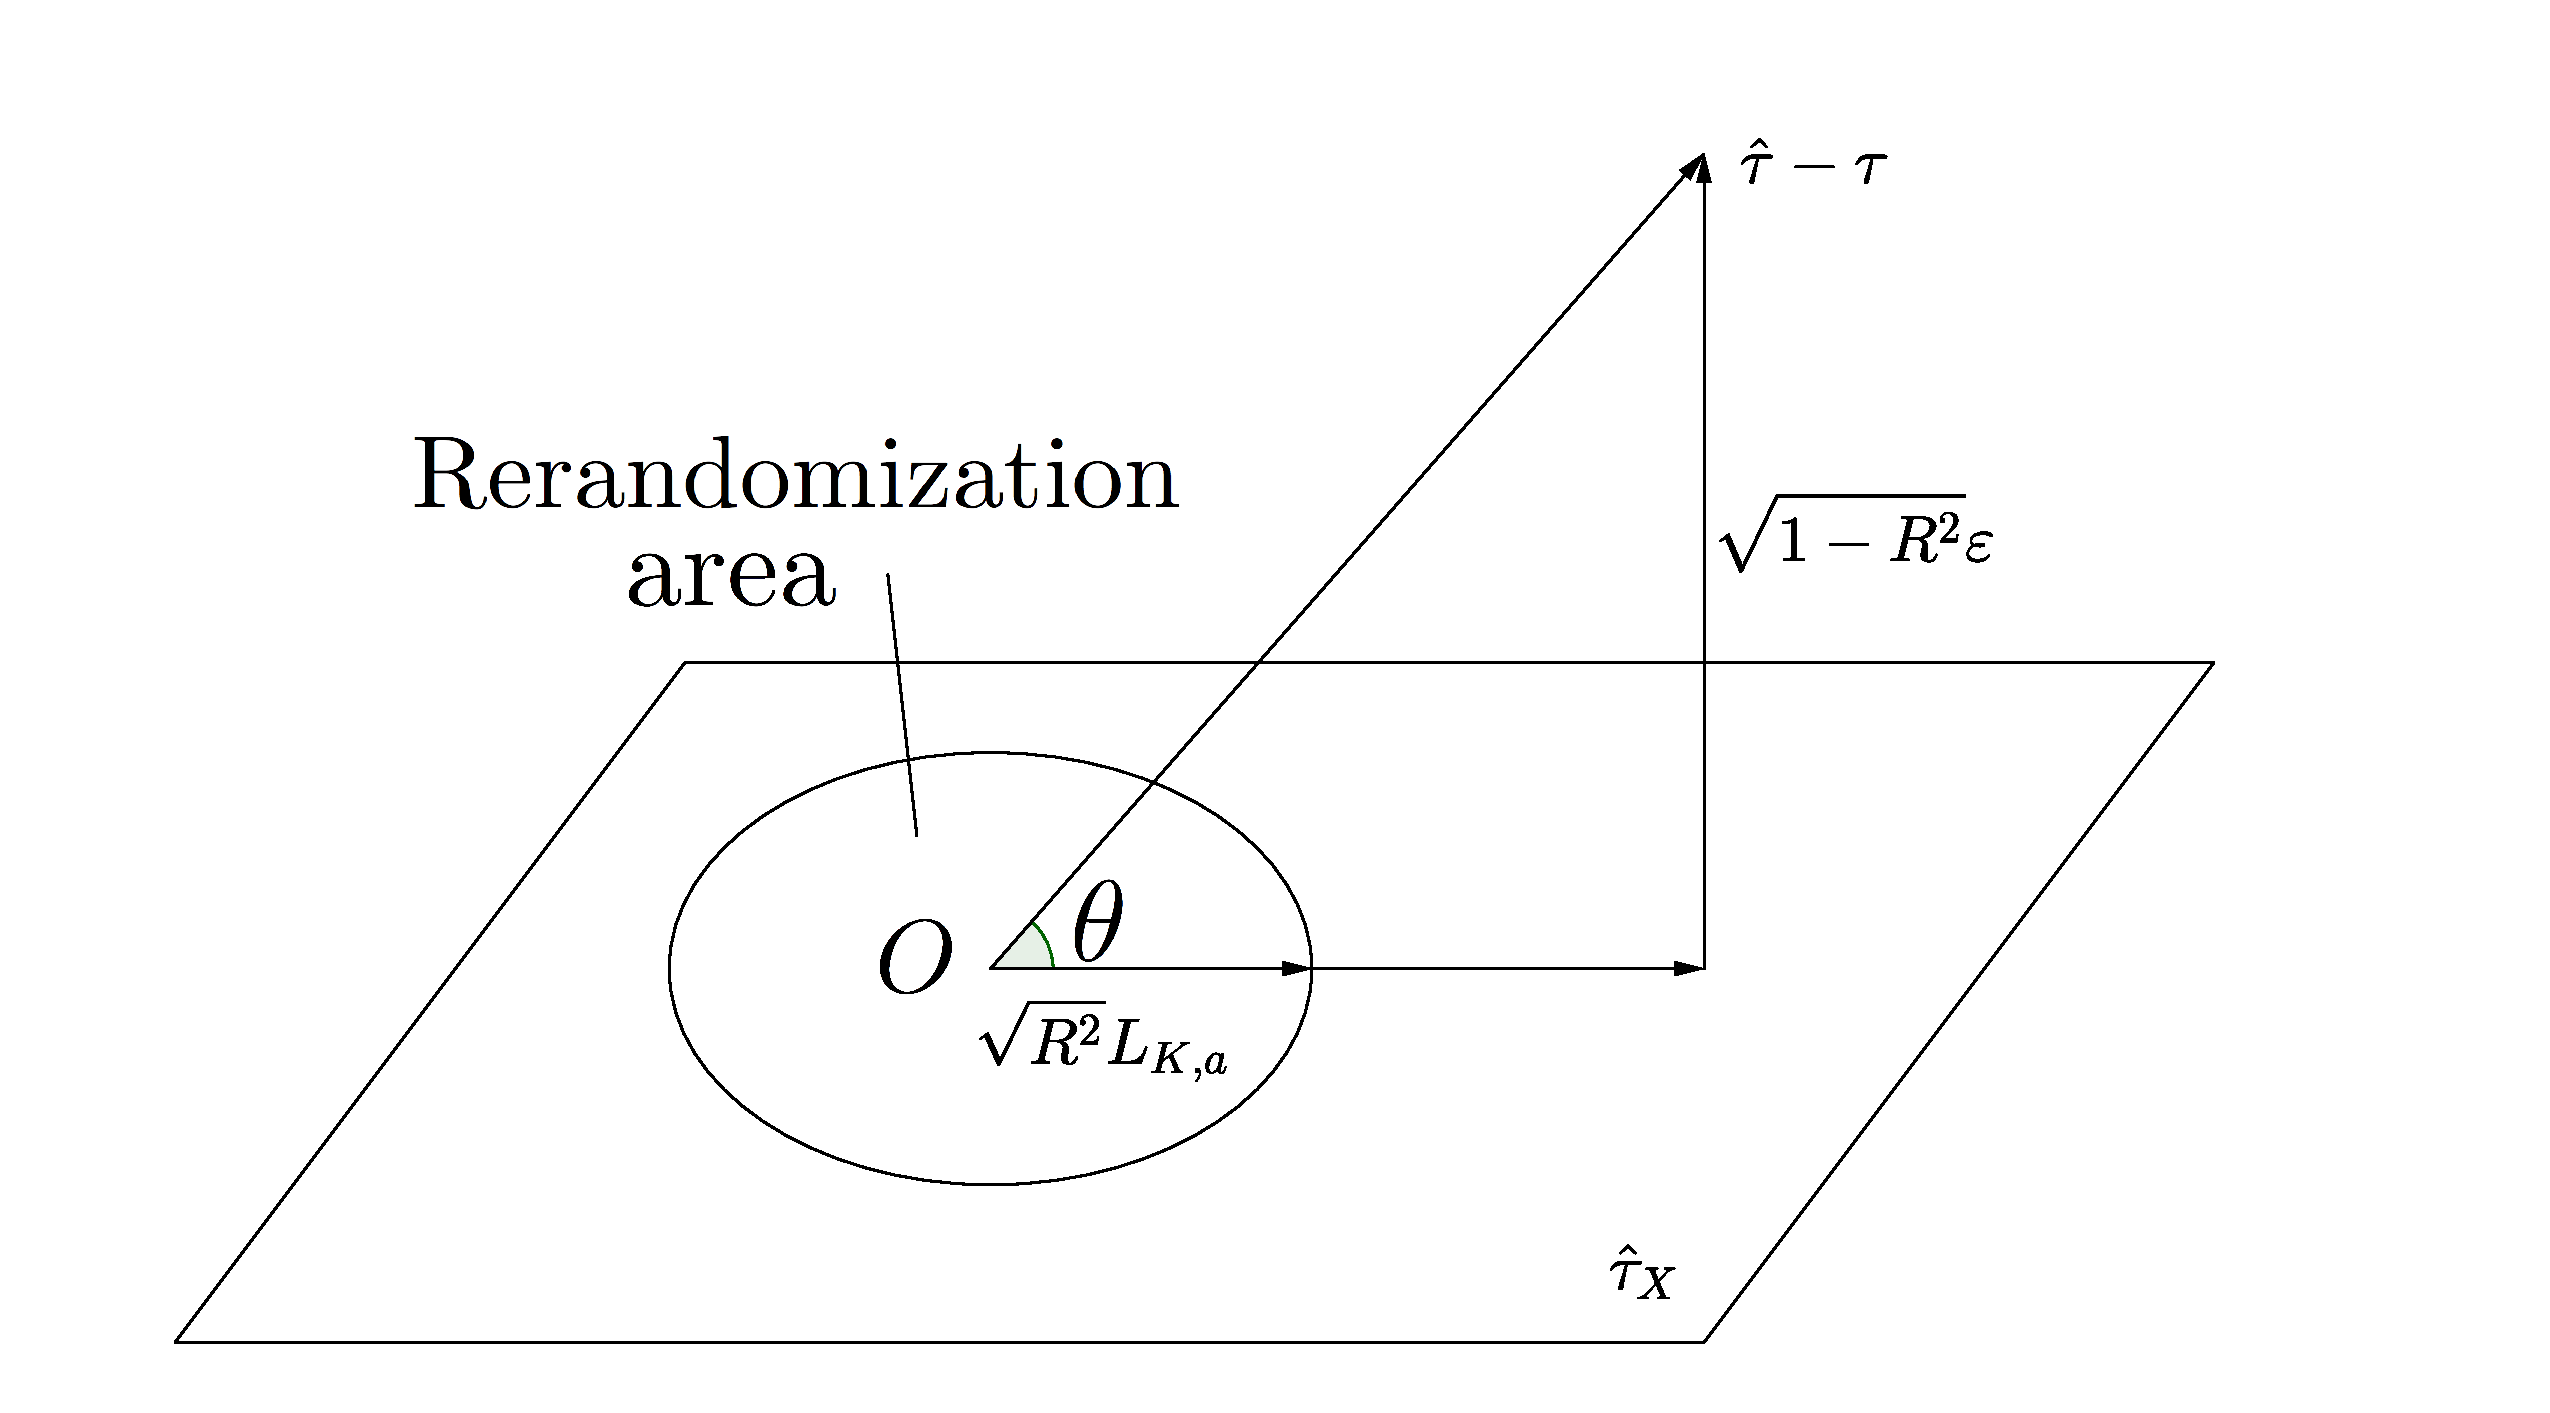
\includegraphics[width = 0.9\textwidth]{figures/rem_geometry.pdf}
\caption{再随机化下$\hat\tau$渐近分布的几何解释}\label{fig::geometry-rem}
\end{figure}


当阈值 $a  = \infty$ 时，该渐进分布退化为完全随机化下的分布形式：
$$
\hat{\tau} - \tau \asim \sqrt{ \var(\hat \tau) } \varepsilon .
$$
当阈值 $a$ 极接近于零时，分布形式变为：
$$
\hat{\tau} - \tau \asim \sqrt{ \var(\hat \tau) (1-R^2)} \varepsilon ;
$$
严格证明见 \citet{wang2022rerandomization}。由此可知，在 $a$ 值较小的情况下，再随机化的效率提升效果直接取决于 $R^2$ 的大小。该系数还具有以下等价表达形式。 
\begin{proposition}
\label{prop::rsquared-forms}
在完全随机实验下，
$$
R^2 = \textup{corr}^2(\hat{\tau}, \hat{\tau}_X   )
= \frac{  n_1^{-1}  S^2(1\mid X) + n_0^{-1} S^2(0\mid X) - n^{-1} S^2(\tau \mid X) }
{ n_1^{-1}  S^2( 1 ) + n_0^{-1} S^2( 0 ) - n^{-1} S^2( \tau  )},
$$
其中$\{S^2( 1 ) , S^2( 0 ), S^2( \tau  )\}$是$\{ Y_i(1), Y_i(0), \tau_i \}_{i=1}^n$的有限总体方差，$\{S^2( 1 \mid x ) , S^2( 0 \mid x ), S^2( \tau  \mid x )\}$是它们分别在线性空间$(1, X_i)$上投影后的有限总体方差；线性投影的定义见第\ref{sec::sampleOLS}节。 
%\footnote{For example, the linear projection of $Y_i(1)$ on $(1,X_i)$ is $\alpha_1 + \beta_1 X_i$ where 
%$$
%(\alpha_1, \beta_1) = \arg \min_{a,b} \sumn \{  Y_i(1) - a - b\tran X_i\}^2.
%$$
%}
在个体因果效应恒定、即$\tau_i = \tau$的假设下，$R^2 $简化为$S^2(0\mid X) / S^2( 0 ) $，也就是$Y_i(0)$与$X_i$的有限总体多重相关系数平方。
\end{proposition}

命题\ref{prop::rsquared-forms}的证明留作习题\ref{para::r2-cre}。 

当$ 0 < a <\infty$时，$\hat{\tau}$的渐近分布更复杂，却更集中在$\tau$附近，所以再随机化下的均值差$\hat{\tau}$比完全随机实验下更精确。 


若忽略再随机化设计，仍根据\cite{Neyman:1923}的方差公式和正态近似构造置信区间，即使个体因果效应恒定，区间也会过度保守，对$\tau$产生过高覆盖率。\citet{li2018asymptotic}提出根据定理\ref{thm::remasymptotics}构造置信区间。这里略去细节，第\ref{sec::unification-rem-regadj}节再回到推断问题。 
 



\section{回归调整}

当处理组与对照组样本量相等时，再随机化下的估计量偏差较小且渐进无偏；然而当两组样本量不等时，再随机化可能引入一定偏差。该点亦可从几何角度加以解释：在两组样本量不等时，正交分量的权重改变可能导致估计量方向调整幅度变大，从而引入更多偏差。 

\subsection{再随机化与后分层法的关联}\label{sec::covariate-adjusted-frt-intro}


协变量$\bm{X}$均为固定值；在$\HF$下，观测结果也全部固定。因此，可以模拟任意检验统计量$T = T(\bm{Z}, \bm{Y}, \bm{X})$的分布，并计算$p$值。有额外协变量时，FRT 的基本思想仍然不变。  


构造统计量有两种一般策略，此前习题\ref{hw::frt-covariates}已提示这两种思路。下面采用\citet{zhao2020caFRT}的术语作概括。 


\begin{definition}
[协变量调整 FRT 的伪结果策略]
\label{def::pseudo-y-frt}
可以根据统计模型拟合后的残差构造统计量。将$Y_i$对$X_i$作回归，得到残差$\hat \varepsilon_i$，然后将$\hat \varepsilon_i$视为伪结果来构造检验统计量。
\end{definition}



\begin{definition}
[协变量调整 FRT 的模型输出策略]
\label{def::model-out-frt}
可以将回归系数作为统计量。将$Y_i$对$(Z_i, X_i)$作回归，以$Z_i$的系数作为检验统计量。
\end{definition}

 

在定义\ref{def::pseudo-y-frt}的伪结果策略中，将$Y_i$对$X_i$作回归时不应加入处理$Z_i$，以保证原结果满足$\HF$时，伪结果也满足$\HF$。定义\ref{def::model-out-frt}的模型输出策略则在$Y_i$对$(Z_i, X_i)$的回归中加入处理$Z_i$，因为要用$Z_i$的系数衡量偏离$\HF$的程度。计算上，第一种策略只需回归一次，第二种策略则需反复回归。 

这里的“回归”泛指线性回归、逻辑回归，甚至机器学习算法。在$\HF$下，这两类策略产生的任意统计量都给出有限样本精确的 FRT，但在备择假设下表现可能不同。本节余下部分回顾若干基于 OLS 的统计量。 



\subsection{协方差分析及其推广}\label{sec::ancova}

现在转向直接估计平均因果效应$\tau$，并调整观测协变量。 

历史上，\citet{fisher1925statistical}提出用协方差分析（ANCOVA）提高估计效率。它至今仍是许多领域的标准方法：将$Y_i$对$(1, Z_i, X_i)$作 OLS 回归，取$Z_i$的系数估计$\tau$。将 Fisher 的 ANCOVA 估计量记为$\hat{\tau}_\textsc{F}$。 


曾任伯克利统计系教授的 David A. Freedman 在\citet{Neyman:1923}的潜在结果框架下重新分析了 Fisher 的 ANCOVA。\citet{freedman2008regression_a, freedman2008regression_b}发现以下负面结果：
\begin{enumerate}
[(1)]
\item
$\hat{\tau}_\textsc{F}$有偏，而简单均值差$\hat{\tau}$无偏。
\item 
当$n_1\neq n_0$时，$\hat{\tau}_\textsc{F}$的渐近方差甚至可能大于$\hat{\tau}$的渐近方差。
\item 
在完全随机实验下，OLS 给出的标准误不是$\hat{\tau}_\textsc{F}$真实标准误的一致估计。   
\end{enumerate}


曾在伯克利攻读博士的 Winston Lin 在论文中回应了 Freedman 的批评。\citet{lin2013}得到了以下正面结论：
\begin{enumerate}
[(1)]
\item
大样本下，$\hat{\tau}_\textsc{F}$的偏差较小，并随着样本量趋于无穷而趋于零。
\item
将$Y_i$对$(1, Z_i, X_i, Z_i\times X_i)$作 OLS 回归，以$Z_i$的系数作为估计量，可以同时改进$\hat{\tau}$与$\hat{\tau}_\textsc{F}$的渐近效率。用$\hat{\tau}_\textsc{L}$表示\citet{lin2013}的估计量。此外，EHW 标准误是在完全随机实验下$\hat{\tau}_\textsc{L}$真实标准误的保守估计。 
\item
将$Y_i$对$(1, Z_i, X_i)$作 OLS 回归时，$\hat{\tau}_\textsc{F}$的 EHW 标准误\footnote{不含协变量时，HC2 修正得到的方差估计与\citet{Neyman:1923}的经典估计完全相同，见习题\ref{hw::neyman-ols-nox}。为统一处理，也可以对\citet{lin2013}的协变量调整估计量使用 HC2 修正。当协变量数相对样本量较小、且协变量无离群值时，EHW 标准误的不同变体表现相近；协变量较多或存在离群值时，变体可能优于原方法。此时\citet{lei2018regression}推荐 HC3 变体。}是在完全随机实验下$\hat{\tau}_\textsc{F}$真实标准误的保守估计。 
\end{enumerate}


\subsubsection{\citet{lin2013}结论的直观解释}


\citet{Neyman:1923}的结论表明，均值差估计量$\hat{\tau}$的方差依赖于潜在结果的方差。直观上，降低潜在结果的方差，就能降低估计量的方差。考虑一类线性调整估计量
\begin{eqnarray} 
\hat{\tau}(\beta_1, \beta_0) &=& n_1^{-1} \sumn Z_i(Y_i - \beta_1\tran X_i) - n_0^{-1} \sumn (1-Z_i) (Y_i - \beta_0\tran X_i)  \label{eq::linear-adj-1}\\
&=& \left\{  \hat{\bar{Y}}(1) - \beta_1\tran \hat{\bar{X} }(1) \right\}  -  \left\{   \hat{\bar{Y}}(0) - \beta_0\tran \hat{\bar{X} }(0) \right\},
\label{eq::linear-adj-2}
\end{eqnarray}
其中$\{ \hat{\bar{Y}}(1), \hat{\bar{Y}}(0) \}$为结果的样本均值，$\{ \hat{\bar{X} }(1), \hat{\bar{X} }(0)\}$为协变量的样本均值。估计量$\hat{\tau}(\beta_1, \beta_0)$通过对潜在结果残差化来降低$\hat\tau$的方差；取$\beta_1 = \beta_0 = 0$时，它退化为$\hat\tau$。由于$\bar{X}  = 0.$，对任意固定$\beta_1$和$\beta_0$，其期望都为$\tau$。我们希望选择$(\beta_1, \beta_0)$，使$\hat{\tau}(\beta_1, \beta_0)$的方差最小。这本质上是调整后潜在结果$\{ Y_i(1) - \beta_1\tran X_i  , Y_i(0) - \beta_0\tran  X_i \}_{i=1}^n $的均值差。应用\citet{Neyman:1923}的结论，方差为
$$
\var\{ \hat{\tau}(\beta_1, \beta_0) \} = \frac{ {S}^2(1; \beta_1) }{ n_1 } + \frac{ {S}^2(0; \beta_0) }{ n_0 }
- \frac{  S^2(\tau; \beta_1, \beta_0)  }{ n },
$$
其中$ {S}^2(z; \beta_z)$（$(z=1,0)$）与$S^2(\tau; \beta_1, \beta_0)$分别为调整后潜在结果及个体因果效应的有限总体方差；保守方差估计为
$$
\hat{V}( \beta_1, \beta_0 ) = \frac{ \hat{S}^2(1; \beta_1) }{ n_1 } + \frac{ \hat{S}^2(0; \beta_0) }{ n_0 },
$$
其中
\begin{eqnarray*}
\hat{S}^2(1; \beta_1) &=& (n_1-1)^{-1} \sumn Z_i  ( Y_i - \gamma_1 - \beta_1\tran  X_i )^2,\\ 
\hat{S}^2(0; \beta_0) &=& (n_0-1)^{-1} \sumn (1-Z_i)  ( Y_i - \gamma_0 - \beta_0\tran  X_i )^2
\end{eqnarray*}
是调整后潜在结果的样本方差，$\gamma_1$、$\gamma_0$分别是处理组中$Y_i - \beta_1\tran  X_i$与对照组中$Y_i   - \beta_0\tran  X_i $的样本均值。要使$\hat{V}( \beta_1, \beta_0 )$最小，需要求解两个 OLS 问题\footnote{也可最小化$\hat{\tau}(\beta_1, \beta_0) $的真实方差，详见习题\ref{hw::compare-true-variance}。}：
$$
\min_{\gamma_1 , \beta_1 }
\sumn Z_i  ( Y_i - \gamma_1 - \beta_1\tran  X_i )^2,\quad
\min_{\gamma_0 , \beta_0 }
\sumn (1-Z_i)  ( Y_i - \gamma_0 - \beta_0\tran  X_i  )^2.
$$
分别在处理组和对照组将$Y_i$对$X_i$作 OLS 回归，得到$( \hat{\gamma}_1, \hat{\beta}_1 )$和$( \hat{\gamma}_0, \hat{\beta}_0 )$。最终估计量为
\begin{eqnarray*}
 \hat{\tau}( \hat{\beta}_1, \hat{\beta}_0) &=& n_1^{-1} \sumn Z_i(Y_i - \hat{\beta}_1\tran  X_i) 
- n_0^{-1} \sumn (1-Z_i)  (Y_i - \hat{\beta}_0\tran  X_i) \\
&=&\left\{  \hat{\bar{Y}}(1) - \hat \beta_1\tran \hat{\bar{X} }(1) \right\}  
-  \left\{   \hat{\bar{Y}}(0) - \hat \beta_0\tran \hat{\bar{X} }(0) \right\} . 
\end{eqnarray*}
由 OLS 拟合的性质（见\eqref{eq::OLS-mean-data}），
$$
\hat{\bar{Y}}(1) =  \hat{\gamma}_1 + \hat{\beta}_1\tran  \hat{\bar{X} }(1),\quad
\hat{\bar{Y}}(0) =  \hat{\gamma}_0 + \hat{\beta}_0\tran  \hat{\bar{X} }(0).
$$
故可将估计量改写为
\begin{equation}
\label{eq::lin-intercepts}
 \hat{\tau}( \hat{\beta}_1, \hat{\beta}_0)  =  \hat{\gamma}_1 - \hat{\gamma}_0  
\end{equation}
\eqref{eq::lin-intercepts}中的等价形式表明，$ \hat{\tau}( \hat{\beta}_1, \hat{\beta}_0) $也可以通过下面的一次 OLS 回归得到。




\begin{proposition}\label{prop::lin-ols}
\eqref{eq::lin-intercepts}中的估计量$ \hat{\tau}( \hat{\beta}_1, \hat{\beta}_0) $，等于将$Y_i$对$(1, Z_i, X_i, Z_i\times X_i)$作 OLS 回归得到的$Z_i$系数，即此前介绍的\citet{lin2013}估计量$\hat{\tau}_\textsc{L}$。 
\end{proposition}

命题\ref{prop::lin-ols}是一个纯粹的线性代数事实，证明留作习题\ref{para::lin-ols-covadj}。 


根据以上讨论，$\hat{\tau}_\textsc{L}$的保守方差估计量为
\begin{eqnarray*}
\hat{V}(  \hat{\beta}_1, \hat{\beta}_0 ) 
%= \frac{ \hat{S}^2(1; \hat{\beta}_1) }{ n_1 } + \frac{ \hat{S}^2(0; \hat{\beta}_0) }{ n_0 }
&=& \frac{1}{n_1(n_1 - 1)} \sumn Z_i  ( Y_i - \hat{\gamma}_1 - \hat{\beta}_1\tran  X_i  ) ^2 \\
&& \qquad + \frac{1}{n_0(n_0 - 1)} \sumn (1-Z_i)  ( Y_i - \hat{\gamma}_0 - \hat{\beta}_0\tran  X_i )^2.
\end{eqnarray*}
\citet{lin2013}通过较复杂的推导进一步证明，命题\ref{prop::lin-ols}中 OLS 回归给出的 EHW 标准误，与由$\hat{V}(  \hat{\beta}_1, \hat{\beta}_0 ) $计算的标准误几乎相同，后者是在完全随机实验下$\hat{\tau}_\textsc{L}$真实标准误的保守估计。直观上，这是因为我们未假定线性模型设定正确，而 EHW 标准误对模型误设具有稳健性。 



上述讨论有一个微妙之处：方差公式$\var\{ \hat{\tau}(\beta_1, \beta_0) \} $适用于固定$(\beta_1, \beta_0)$，而估计量$ \hat{\tau}( \hat{\beta}_1, \hat{\beta}_0) $使用了两个估计系数$( \hat{\beta}_1, \hat{\beta}_0) $。估计系数的额外不确定性可能使最终估计量产生有限样本偏差。\citet{lin2013}证明，这一问题在渐近意义下消失，因为$ \hat{\tau}( \hat{\beta}_1, \hat{\beta}_0) $与$ \hat{\tau}( \tilde{\beta}_1, \tilde{\beta}_0) $表现相似，其中$\tilde{\beta}_1$、$\tilde{\beta}_0$分别是$\hat{\beta}_1$、$ \hat{\beta}_0$的极限。直观上，$ \hat{\tau}( \hat{\beta}_1, \hat{\beta}_0) $与$ \hat{\tau}( \tilde{\beta}_1, \tilde{\beta}_0) $之差依赖于
$$
(\hat{\beta}_z - \tilde{\beta}_z)\tran \hat{\bar{X} }(z) ,\quad (z=0,1) 
$$
它是两个小阶量的乘积。需要注意，渐近理论要求较大样本量，以及潜在结果和协变量满足一定正则条件。在有限样本中，$\hat{\beta}_1$和$\hat{\beta}_0$估计带来的额外不确定性甚至可能使回归调整有害。 




\subsubsection{通过预测潜在结果理解\citet{lin2013}的估计量}
\label{sec::understand-lin-predict}
 
\begin{table}
\centering
\caption{再随机化与协变量不平衡的调整}\label{tb::predict-po-ols}
\begin{tabular}{cccccc}
\hline 
$X$ & $Z$ & $Y(1)$ & $Y(0)$ &  $\hat{Y}(1)$ & $\hat{Y}(0)$ \\
\hline
$X_1 $ & 1 & $Y_1(1)$ & ? & $\hat{\mu}_1(X_1 )$ & $\hat{\mu}_0(X_1)$ \\
\vdots \\
$X_{n_1}$ & 1 & $Y_{n_1}(1)$ & ? & $\hat{\mu}_1(X_{n_1})$ & $\hat{\mu}_0(X_{n_1})$ \\
$X_{n_1 + 1}$ & 0 & ? & $Y_{n_1+1}(0)$ & $\hat{\mu}_1(X_{n_1+1})$ & $\hat{\mu}_0(X_{n_1+1})$ \\
\vdots \\
$X_{n}$ & 0 & ? & $Y_{n}(0)$ & $\hat{\mu}_1(X_{n})$ & $\hat{\mu}_0(X_{n})$ \\
\hline 
\end{tabular}
\end{table}


 
可以把\citet{lin2013}的估计量看作基于潜在结果对协变量 OLS 拟合的{\it 预测型估计量}。用处理组数据，建立由$X$预测$Y(1)$的模型：
\begin{eqnarray}
\label{eq::pred-y1-linear}
\hat{\mu}_1(X) = \hat{\gamma}_1 + \hat{\beta}_1\tran X.
\end{eqnarray}
类似地，用对照组数据，建立由$X$预测$Y(0)$的模型：
\begin{eqnarray}
\label{eq::pred-y0-linear}
\hat{\mu}_0(X)= \hat{\gamma}_0 + \hat{\beta}_0\tran X . 
\end{eqnarray}
表\ref{tb::predict-po-ols}说明潜在结果的预测。若只预测缺失的潜在结果，可得预测型估计量
\begin{eqnarray}\label{eq::predictive-estimator-generic}
\hat{\tau}_\text{pred} = n^{-1} \left\{   \sum_{Z_i=1}Y_i + \sum_{Z_i=0}\hat{\mu}_1(X_i) - \sum_{Z_i=1} \hat{\mu}_0(X_i) - \sum_{Z_i=0} Y_i     \right\} .
\end{eqnarray}
可验证，采用\eqref{eq::pred-y1-linear}与\eqref{eq::pred-y0-linear}时，这个预测型估计量等于\citet{lin2013}的估计量：
\begin{eqnarray}
\label{eq::predictiveestimator}
\hat{\tau}_\text{pred} = \hat{\tau}_\textsc{L}.
\end{eqnarray}
若预测所有潜在结果，包括已经观测到的结果，则得到{\it 投影型估计量}：
\begin{eqnarray}\label{eq::projective-estimator-generic}
\hat{\tau}_\text{proj} = n^{-1}  \sumn \{ \hat{\mu}_1(X_i) - \hat{\mu}_0(X_i)    \}.
\end{eqnarray}
可验证，采用\eqref{eq::pred-y1-linear}与\eqref{eq::pred-y0-linear}时，投影型估计量也等于\citet{lin2013}的估计量：
\begin{eqnarray}
\label{eq::projectiveestimator}
\hat{\tau}_\text{proj} = \hat{\tau}_\textsc{L}.
\end{eqnarray}
\eqref{eq::predictiveestimator}与\eqref{eq::projectiveestimator}的证明留作习题\ref{para::predictiveestimator}。 


“预测型”与“投影型”的术语来自抽样调查文献\citep{firth1998robust, ding2018causal}。在更一般的公式\eqref{eq::predictive-estimator-generic}和\eqref{eq::projective-estimator-generic}中，也可使用其他潜在结果预测器。为说明与\citet{lin2013}估计量的联系，这里采用线性预测。预测器$\hat{\mu}_1(X)$与$\hat{\mu}_0(X)$可以非常一般，包括更复杂的机器学习算法。但构造点估计只是分析完全随机实验的第一步，更重要的第二步是量化估计量的不确定性，这取决于潜在结果预测器的性质。不过，无需额外理论分析，总可将\eqref{eq::predictive-estimator-generic}和\eqref{eq::projective-estimator-generic}作为 FRT 的检验统计量。 
 
 
\subsubsection{通过调整协变量不平衡理解\citet{lin2013}的估计量}
\label{sec::lin=adjustingforimbalance}

线性调整估计量可等价地写成
\begin{eqnarray}\label{eq::linear-covariate-imbalance}
%\hat{\tau}(\gamma) = 
\hat{\tau}(\beta_1, \beta_0) = \hat{\tau} - \gamma\tran \hat{\tau}_X 
\end{eqnarray}
其中$\gamma =\frac{n_0}{n} \beta_1 + \frac{n_1}{n} \beta_0$，因而也可写为$\hat{\tau}(\gamma) = 
\hat{\tau}(\beta_1, \beta_0) .$。类似地，\citet{lin2013}的估计量有等价形式
\begin{eqnarray}\label{eq::lin-covariate-imbalance}
\hat{\tau}_\textsc{L} = \hat{\tau} - \hat \gamma\tran \hat{\tau}_X ,
\end{eqnarray}
其中$\hat \gamma =\frac{n_0}{n} \hat \beta_1 + \frac{n_1}{n} \hat  \beta_0$。\eqref{eq::linear-covariate-imbalance}与\eqref{eq::lin-covariate-imbalance}的证明留作习题\ref{para::reg-covariate-imbalance}。\eqref{eq::linear-covariate-imbalance}与\eqref{eq::lin-covariate-imbalance}正是“调整协变量不平衡”的数学表达：从原均值差中减去协变量均值差的某个线性组合。在完全随机实验下，$\hat{\tau} $与$\hat{\tau}_X $相关，因此适当选择$\gamma$作协变量调整，就可降低$\hat{\tau} $的方差。\eqref{eq::linear-covariate-imbalance}和\eqref{eq::lin-covariate-imbalance}还有一个有意思的性质：最终估计量只依赖$\gamma$或$\hat \gamma$，因此$\beta$系数的选择并不唯一。\citet{li2019rerandomization}指出了这一简单事实。所以，\citet{lin2013}的估计量只是最优估计量之一；但它容易通过标准 OLS 与 EHW 标准误实现，因此本书主要介绍它。 



\subsection{关于回归调整的补充说明}


\subsubsection{再随机化与回归调整的对偶性}\citet{li2018asymptotic}指出，再随机化与\citet{lin2013}的回归调整分别在实验设计阶段和分析阶段使用协变量，二者具有对偶关系。具体而言，$a$较小时，再随机化下$\hat{\tau}$的渐近分布与完全随机实验下$\hat{\tau}_\textsc{L}$的渐近分布几乎相同。因此，再随机化在设计阶段使用协变量，\citet{lin2013}的回归调整在分析阶段使用协变量；当$a$较小时，二者几乎取得相同的渐近效率增益。 


 \subsubsection{回归调整与后分层的等价性}若离散协变量$C_i$有$K$个类别，可构造$K-1$个中心化的虚拟变量
$$
X_i = ( I(C_i=1) - \pi_{[1]}, \ldots,   I(C_i=K-1) - \pi_{[K-1]})
$$
其中$\pi_{[k]}$为满足$C_i = k$的单位比例。此时\citet{lin2013}的回归调整等价于后分层，见下面的命题。 

\begin{proposition}
\label{prop::lin=ps-discrete}
基于$X_i$的$\hat{\tau}_\textsc{L}$与基于$C_i$的后分层估计量$\hat{\tau}_\textsc{PS}$在数值上完全相同（见第\ref{sec::poststra-cre}节）。 
\end{proposition}


命题\ref{prop::lin=ps-discrete}的证明留作习题\ref{para::lin=ps-discrete}。 


\subsubsection{作为协变量调整$\hat \tau(\beta_1, \beta_0)$特例的双重差分}\label{sec::difference-in-difference-CRE}
许多研究中的重要协变量$X$是处理前的滞后结果。例如，教育研究中，结果$Y$是后测成绩，协变量$X$是前测成绩；职业培训研究中，结果$Y$是培训后的对数工资，协变量$X$是培训前的对数工资。以滞后结果$X$为协变量，一种常用方法是{\it 增益分数}或{\it 双重差分}估计量，即在\eqref{eq::linear-adj-1}和\eqref{eq::linear-adj-2}中固定$\beta_1 = \beta_0=1$：
\begin{eqnarray*}
\hat{\tau}(1,1) &=& n_1^{-1} \sumn Z_i(Y_i -   X_i) - n_0^{-1} \sumn (1-Z_i) (Y_i -   X_i) \\
&=& \left\{   \hat{\bar{Y}}(1) - \hat{\bar{Y}}(0) \right\} -  \left\{   \hat{\bar{X} }(1) - \hat{\bar{X} }(0) \right\} .
\end{eqnarray*}
$\hat{\tau}(1,1) $的第一种形式说明了{\it 增益分数}这一名称，因为它本质上是增益分数$g_i = Y_i - X_i$的均值差。$\hat{\tau}(1,1) $的第二种形式说明了{\it 双重差分}这一名称，因为它是两个均值差之差。它不同于\citet{lin2013}的估计量：它事先固定$\beta_1 = \beta_0=1$，而\citet{lin2013}的估计量需要估计两个$\beta$。$\hat{\tau}(1,1) $是无偏的，其保守方差估计量为
\begin{eqnarray*}
\hat{V}( 1,1 ) 
&=& \frac{1}{n_1(n_1 - 1)} \sumn Z_i  \{ g_i - \hat{\bar{g}}(1)   \}^2 \\
& & \qquad + \frac{1}{n_0(n_0 - 1)} \sumn (1-Z_i)  \{ g_i - \hat{\bar{g}}(0)   \}^2,
\end{eqnarray*}
其中$\hat{\bar{g}}(1)$和$ \hat{\bar{g}}(0)$分别为处理组与对照组的增益分数$g_i = Y_i - X_i$的样本均值。若滞后结果能很好地预测结果，增益分数$g_i = Y_i - X_i$的方差往往远小于结果本身的方差；此时$\hat{\tau}(1,1) $能显著降低简单结果均值差的方差。详见习题\ref{hw::did-CRE}。 


理论上，在大样本中，\citet{lin2013}的估计量始终比$\hat{\tau}(1,1)$更有效率。但\citet{lin2013}的估计量有有限样本偏差，而$\hat{\tau}(1,1)$始终无偏。   





\subsection{推广到分层随机实验}\label{sec::covariate-SRE}


实验可能按离散变量$C$分层，同时观测到额外协变量$X$。若每层都足够大，可在层内计算\citet{lin2013}的估计量$\hat{\tau}_{\textsc{L},[k]}$，再合成为
$$
\hat{\tau}_{\textsc{L},\textsc{S}} = \sum_{k=1}^K \pi_{[k]} \hat{\tau}_{\textsc{L},[k]} . 
$$
保守方差估计量为
$$
\hat{V}_{\textsc{L},\textsc{S}} =  \sum_{k=1}^K \pi_{[k]}^2 \hat{V}_{\textsc{ehw},[k]},
$$
其中$\hat{V}_{\textsc{ehw},[k]}$是在第$k.$层内，将结果对截距、处理指标、协变量及处理与协变量交互项作 OLS 回归得到的 EHW 方差估计。协变量必须按各层自己的均值进行中心化。
 

\section{统一、组合与比较}
\label{sec::unification-rem-regadj}


\citet{li2019rerandomization}统一了相关文献，证明再随机化可以与回归调整结合：在设计阶段进行再随机化后，分析阶段可使用\citet{lin2013}的估计量及 EHW 标准误。这种结合既改善设计阶段的协变量平衡，也提高分析阶段的估计效率。 




表\ref{tb::rerandomization-regression}概括了从\citet{Neyman:1923}到\citet{li2019rerandomization}的研究。箭头 1 表示完全随机实验中协变量调整的效率增益：渐近地，$\hat\tau_\textsc{L}$的方差小于$\hat\tau$。箭头 2 表示再随机化的效率增益：渐近地，$\hat{\tau}$在再随机化下的分位区间窄于完全随机实验。箭头 3 和 4 表示将再随机化与回归调整相结合的收益。



\begin{table}
\centering
\caption{随机实验的设计与统计分析}\label{tb::design-analysis-2x2}
\label{tb::rerandomization-regression}
\begin{tabular}{c|cccc}
\hline 
  & & & 统计分析 & \\
  \hline 
  & CRE & $\hat\tau$ \citep{Neyman:1923} &  $\stackrel{1}{\longrightarrow}$  &  $\hat\tau_\textsc{L}$ \citep{lin2013} \\
  实验设计&  &  $2\Big\downarrow$ && $  \Big\downarrow 4$ \\
  & 再随机化 & $\hat\tau$  \citep{li2018asymptotic} &  $\stackrel{3}{\longrightarrow}$  &$\hat\tau_\textsc{L}$ \citep{li2019rerandomization}  \\
  \hline 
\end{tabular}
\end{table}



 

\section{模拟}
\label{sec::rem-reg-simulation}

\citet{angrist2009incentives}在加拿大某大学开展实验，评价提高一年级学生学业表现的不同策略。这里使用原数据的一个子集，比较对照组与同时获得学业支持服务及良好成绩经济奖励的处理组。结果是第一学年末的 GPA。缺失结果以观测均值填补，这种做法有一定任意性（见习题\ref{hw::missing-y-experiments}）。两个协变量为性别和基线 GPA。

\begin{lstlisting}
angrist   = read.dta("star.dta")
angrist2  = subset(angrist, control == 1||sfsp == 1)
## imputing missing outcomes
y = angrist2$GPA_year1
meany    = mean(y, na.rm = TRUE)
y = ifelse(is.na(y), meany, y)
z = angrist2$sfsp 
x = angrist2[, c("female", "gpa0")]
\end{lstlisting}


以下代码演示了两种估计量的统计性质： 
\begin{lstlisting}
> ## unadjusted estimator
> fit_unadj = lm(y ~ z)
> ace_unadj = coef(fit_unadj)[2]
> se_unadj  = sqrt(hccm(fit_unadj, type = "hc2")[2, 2])
> 
> ## regression adjustment
> x         = scale(x)
> fit_adj   = lm(y ~ z*x)
> ace_adj   = coef(fit_adj)[2]
> se_adj    = sqrt(hccm(fit_adj, type = "hc2")[2, 2])
> 
> res = c(ace_unadj, ace_adj, se_unadj, se_adj)
> dim(res) = c(2, 2)
> t.stat   = res[, 1]/res[, 2]
> p.value  = 2*pnorm(abs(t.stat), lower.tail = FALSE) 
> res      = cbind(res, t.stat, p.value)
> rownames(res) = c("Neyman", "Lin")
> colnames(res) = c("estimate", "s.e.", "t-stat", "p-value")
> round(res, 3)
       estimate  s.e. t-stat p-value
Neyman    0.054 0.076  0.719   0.472
Lin       0.075 0.072  1.036   0.300
\end{lstlisting}
尽管回归调整估计量的标准误小于原始估计量，二者在统计显著性层面并无显著差别。 



还利用此数据集模拟比较表\ref{tb::design-analysis-2x2}中的四种设计与分析策略。分别在处理组和对照组，用结果对协变量拟合二次函数，填补所有缺失潜在结果。为展示再随机化和回归调整的改进，还分别将误差项乘以$0.1$和$0.25$，提高信噪比。利用填补后的科学表，生成 2000 次处理分配，得到观测数据并计算估计量。模拟中的“真实”结果模型非线性，但仍采用线性调整估计，以评价线性模型误设时估计量的性质。 


图\ref{fg::rerandomizationandancova}给出了四种组合的估计值减去真实$\tau$后的小提琴图。\footnote{小提琴图类似箱线图，但两侧各增加一幅旋转后的核密度图。}正如理论预测，所有估计量都近似无偏，再随机化和回归调整均提高效率，而且噪声越小，效果越明显。 

\begin{figure}
\centering
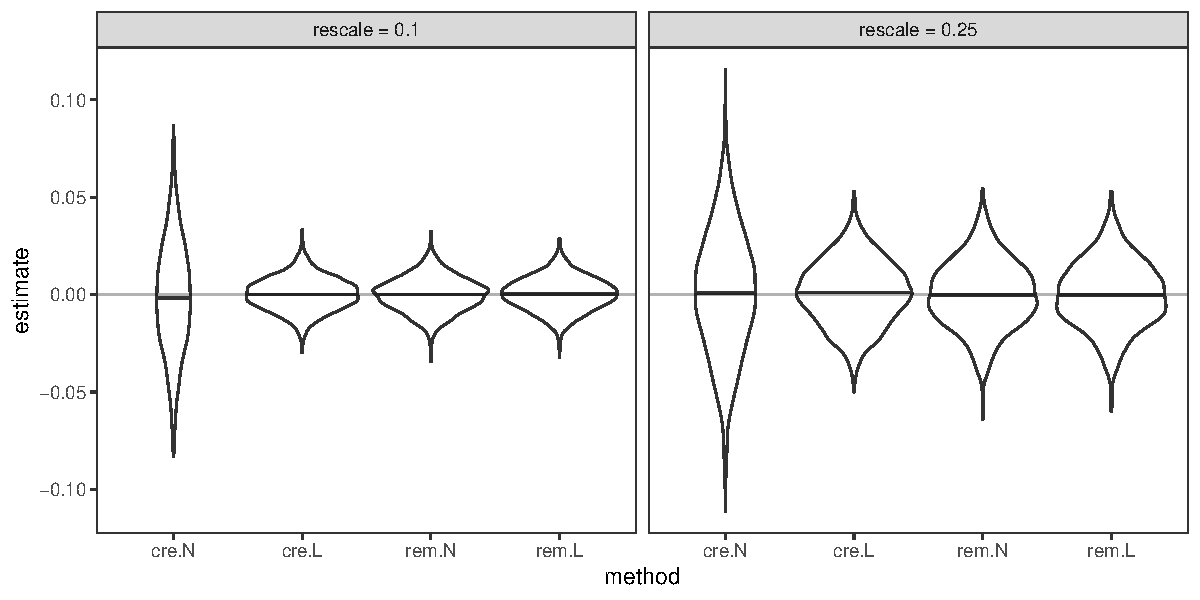
\includegraphics[width = \textwidth]{figures/RemReg_violin.pdf}
\caption{$2000$次蒙特卡洛重复、再随机化阈值$a=0.05$下的模拟} \label{fg::rerandomizationandancova}
\end{figure}


 


\section{结语}

再随机化以马氏距离作为平衡准则，也可将准则推广为$\bm{Z}$与$\bm{X}$的一般函数。例如，对$X_i = (x_{i1}, \ldots, x_{iK})\tran$的每个分量进行边际检验，只有在
\begin{equation}
\label{eq::marginal-testing-rerandomization}
\left | \frac{  \hat{\tau}_{xk} }{   \sqrt{  \frac{n}{n_1 n_0} S_{xk}^2       }  }   \right | \leq  a \quad ( k=1,\ldots, K )
\end{equation}
时才接受$\bm{Z}$，其中$a > 0$为预先指定的常数，$S_{xk}^2$是协变量$x_{ik}$的有限总体方差。例如，$a$可取标准正态分布的某个上分位点。基于准则\eqref{eq::marginal-testing-rerandomization}及其他准则的再随机化理论见\citet{zhao2021no}。 


对于连续结果，Fisher 的 ANCOVA 多年来一直是标准方法。即使线性模型误设，\citet{lin2013}的改进方法也有更好的理论性质。对于二元结果，常将观测结果对截距、处理指标和协变量作逻辑回归，用处理系数估计因果效应。但\citet{freedman2008randomization}表明，这种逻辑回归在潜在结果框架下的性质并不理想。即使模型正确，处理系数刻画的也是条件对数优势比（见第\ref{sec::logistic-regression}节），未必对应所关心的参数；模型错误时，更难解释。由前述讨论可知，若关注平均因果效应，仍可用\citet{lin2013}的估计量分析完全随机实验中的二元结果。\cite{guo2020generalized}推广了\citet{lin2013}的理论，允许在潜在结果框架下用广义线性模型构造平均因果效应估计量。  


\citet{lin2013}理论的其他推广涉及高维协变量。\citet{bloniarz2015lasso}考虑协变量数多于样本量的情形，建议将结果对截距、处理、协变量及交互项的 OLS 拟合，替换为最小绝对收缩与选择算子（LASSO）拟合\citep{tibshirani1996regression}。\citet{lei2018regression}考虑协变量数发散但不要求稀疏的情形，证明在一定正则条件下，\citet{lin2013}的估计量仍一致且渐近正态。\citet{wager2016high}提出用机器学习方法分析高维实验数据。 



\section{作业习题}

\paragraph{再随机化下的 Fisher 随机化检验}\label{hw::FRT-under-REM}

描述再随机化设计下的 Fisher 随机化检验方法。


\paragraph{马氏距离的不变性}\label{para::invariance-M}

证明引理\ref{lemma::invariance-mdistance}。 


\paragraph{再随机化下均值差的偏差性质}\label{hw::unbiasednessof-tauhat-rerandom}

假设从完全随机实验中抽取$\bm{Z} = (Z_1, \ldots, Z_n)$，仅当$\phi(\bm{Z}, \bm{X}) = 1$时接受该分配，其中$\phi$是预先指定的平衡准则。证明，若$n_1 = n_0$且
\begin{eqnarray}
\phi(\bm{Z}, \bm{X}) = \phi(\bm{1}_n-\bm{Z}, \bm{X}), \label{eq::symmetry}
\end{eqnarray}
则$\hat{\tau}$是$\tau$的无偏估计。验证：$n_1 = n_0$时，使用马氏距离的再随机化满足\eqref{eq::symmetry}。举出两个条件不成立时，$\hat{\tau}$对$\tau$有偏的反例。  


注：本题中的$\phi(\bm{Z}, \bm{X}) $可以是一般平衡准则。再随机化是$\phi(\bm{Z}, \bm{X})  =  I(M\leq a) $这一特例。


\paragraph{完全随机化下 $R^2$ 的等价表达}\label{para::r2-cre}

证明命题\ref{prop::rsquared-forms}。 



\paragraph{再随机化下线性调整估计量的方差分解}\label{hw::projection-po-onto-x}



证明
$$
S^2(1\mid X) = S_{Y(1)X} (S_X^2)^{-1} S_{XY(1)}
$$
其中$S_{XY(1)}$是$X_i$与$Y_i(1)$的有限总体协方差，$S_{Y(1)X} = S_{XY(1)}\tran$，$S_X^2$为$X_i$的有限总体协方差矩阵。写出$S^2(0\mid X) $和$S^2(\tau\mid X) .$的类似公式。



\paragraph{比较线性调整估计量族中的真实方差}\label{hw::compare-true-variance} 



证明$\hat{\tau}(\beta_1, \beta_0)$的方差可分解为
$$
\var\{ \hat{\tau}(\beta_1, \beta_0) \} 
=  
\var\{ \hat{\tau}( \tilde{\beta}_1, \tilde{\beta}_0) \}  
+
\var\{ \hat{\tau}(\beta_1, \beta_0) - \hat{\tau}(\tilde{\beta}_1, \tilde{\beta}_0) \}
$$
其中$\tilde{\beta}_1$和$\tilde{\beta}_0$分别是将$Y_i(1)$、$Y_i(0)$对$(1, X_i)$作 OLS 投影时，$X_i$的系数。 



注：\citet[][Example 9]{li2017general}推导了这一分解。由于$\var\{ \hat{\tau}(\beta_1, \beta_0) - \hat{\tau}(\tilde{\beta}_1, \tilde{\beta}_0) \}$始终非负，$\hat{\tau}( \tilde{\beta}_1, \tilde{\beta}_0)$在线性调整估计量族中按真实方差衡量是一个最优选择。   




\paragraph{Lin 回归调整估计量的等价表达}\label{para::lin-ols-covadj}

证明命题\ref{prop::lin-ols}。 

\paragraph{预测型与投影型估计量的等价性}\label{para::predictiveestimator}
证明 \eqref{eq::predictiveestimator} 和 \eqref{eq::projectiveestimator}。 
 
 
 \paragraph{线性调整估计量的代数表达}\label{para::reg-covariate-imbalance}

证明 \eqref{eq::linear-covariate-imbalance} 和 \eqref{eq::lin-covariate-imbalance}。 
 
 
 
\paragraph{ANCOVA 与协变量不平衡调整的关系}
\label{para::ancova-imbalance}

本题给出 ANCOVA 的一个结论，类似于\eqref{eq::lin-covariate-imbalance}。 

证明
$$
\hat{\tau}_\textsc{F} =\hat\tau  - \hat\gamma_\textsc{F}\tran \hat\tau_X,
$$
其中$ \hat\gamma_\textsc{F}$是将$Y_i$对$(1,Z_i, X_i)$作 OLS 回归时$X_i$的系数。 





 \paragraph{完全随机实验的回归调整与后分层}\label{para::lin=ps-discrete}
 
 证明命题\ref{prop::lin=ps-discrete}。 
 
 
注：有时$\hat{\tau}_{\textsc{ps}}$或$ \hat{\tau}_\textsc{L}$未必有良好定义。在这些情形下，把$\hat{\tau}_{\textsc{ps}}$与$ \hat{\tau}_\textsc{L}$视为相等。证明中可忽略这一复杂情况。 
 
%In a completely randomized experiment, we have a binary treatment indicator $Z$, an outcome $Y$, and a discrete covariate $X \in \{  1, \ldots, K \}$. We can use two methods to use covariates to improve estimation efficiency. 
%
%First, we can use the post-stratification estimator, pretending that the experiment is a stratified randomized experiment, conditional on $X$. This estimator is $\hat{\tau}_{\textsc{ps}}$. 
%
%Second, we can create $K-1$ dummy variables $\delta_{1i} = I(X_i=1), \ldots, \delta_{K-1,i} = I(X_i=K-1)$, and use Lin's estimator with covariates $\delta_1,\ldots, \delta_{K-1}$. This estimator is $\hat{\tau}_\textsc{L}$. 
%
%Show that $\hat{\tau}_{\textsc{ps}} = \hat{\tau}_\textsc{L}.$ Note that sometimes $\hat{\tau}_{\textsc{ps}}$ or $ \hat{\tau}_\textsc{L}$ may not be well-defined. In those cases, we treat $\hat{\tau}_{\textsc{ps}}$ and $ \hat{\tau}_\textsc{L}$ as equal. 


 
% \paragraph{Regression adjustment in the Fisher Randomization Test}
%This is a reanalysis of the LaLonde experimental data used in the lecture. In \texttt{FRTlalonde.R}, I conduct the Fisher randomization test using four test statistics. The Fisher randomization test can be more general with at least the following two additional strategies. Under the potential outcomes framework, {\it all potential outcomes and covariates are fixed numbers}. 
%
%
%First, we can use test statistics based on residuals from the linear regression. Run a linear regression of the outcomes on the covariates, and obtain the residuals (i.e., treat the residuals as the pseudo ``outcomes''). Then define the four test statistics based on the residuals. Conduct the Fisher randomization test using these four new test statistics. Report the corresponding $p$-values.
%
%
%Second, we can define the test statistic as the coefficient in the linear regression of the outcomes on the treatment and covariates. Conduct the Fisher randomization test using this test statistic. Report the corresponding $p$-value. 
%
%
%Why the five $p$-values from the above two strategies are exact $p$-values? Justify them. 


\paragraph{完全随机化下差异-差异估计量的性质}\label{hw::did-CRE}

本题补充第\ref{sec::difference-in-difference-CRE}节完全随机实验中双重差分估计量的细节。 

证明$\hat{\tau}(1,1) $是$\tau$的无偏估计，计算其方差，并证明$\hat{V}( 1,1 ) $是$\hat{\tau}(1,1) $真实方差的保守估计。什么情况下有$E\{\hat{V}( 1,1 ) \} = \var\{  \hat{\tau}(1,1)  \}$？



比较$\hat{\tau}(0,0) $与$\hat{\tau}(1,1) $的方差，证明
$$
\var\{ \hat{\tau}(0,0) \}  \geq \var\{  \hat{\tau}(1,1)  \}
$$
成立当且仅当
$$
2 \frac{n_0}{n} \beta_1 + 2\frac{n_1}{n} \beta_0 \geq 1,
$$
其中
$$
\beta_1 = \frac{\sum_{i=1}^n (X_i-\bar{X})\{  Y_i(1)-\bar{Y}(1) \}  }{  \sum_{i=1}^n (X_i-\bar{X})^2 },\quad
\beta_0 = \frac{\sum_{i=1}^n (X_i-\bar{X})\{  Y_i(0)-\bar{Y}(0) \}  }{  \sum_{i=1}^n (X_i-\bar{X})^2 }
$$
分别为将$Y_i(1)$和$Y_i(0)$对$(1,X_i)$作 OLS 回归时$X_i$的系数。 


注：\citet[][page 28]{gerber2012field}讨论了本题在$n_1=n_0.$时的特例。



\paragraph{Penn 奖学金实验的再分析}

 
重新分析宾州奖金实验数据。第\ref{chapter::stratification-poststratification}章的分析使用处理指标、结果和区组指标，现在需要使用其他所有协变量。 

在实验各层内进行回归调整，再合并调整后的估计量，估计平均因果效应。报告点估计、估计标准误和 95\% 基于实验数据，结合协变量进行回归调整并给出统计推断结果，与未调整结果进行比较分析。 
 

\paragraph{缺失结果下的统计推断}\label{hw::missing-y-experiments}

第\ref{sec::rem-reg-simulation}节的数据分析用简单填补法处理缺失结果，这具有一定任意性。 

分别用处理组和对照组的观测均值填补各组缺失结果，结论是否改变？

分别在处理组和对照组将观测结果对协变量作线性回归，用拟合值填补各组缺失结果，结论是否改变？ 

探讨不同缺失结果处理方法对统计推断的影响。 




\paragraph{推荐阅读}

本章标题与\citet{li2019rerandomization}相同，该文分别研究了再随机化和回归调整在随机实验设计与分析阶段中的作用。 


  
 
\chapter{配对实验}
 \label{chapter::mpe}
 
配对实验（Matched-Pairs Experiment, MPE）是随机化实验（SRE）的极端形式：在每个分层内仅有一个处理组单位和一个对照组单位。此时这些分层也被称为“配对”。虽然这种实验形式属于第\ref{chapter::stratification-poststratification}章所述SRE的特殊情况，但它有自己独立的估计与推断方法。此外，它还具有许多新特性，且与第\ref{chapter::matching-obs}章将要讨论的观测研究中的“匹配”策略密切相关。因此我们在此单独设章探讨MPE。 





\section{实验设计及潜在结果}
 
考虑一个有$2n$个单位的实验。若存在可用于预测结果的协变量，则可依据协变量的相似性来配对单位。若协变量为标量，可先对单位按该值排序，再将相邻单位配对。若存在多个协变量，则可计算单位间的两两距离并据此配对。此时配对过程可采用贪婪算法或最优非二分匹配算法实现。贪婪算法会先配对距离最小的两个单位，将其从候选池移除，再对剩余单位重复此过程。最优非二分匹配算法则能将$2n$个单位划分为$n$个二元组，使得每组内距离之和最小。关于MPE计算层面的更多细节可参见\citet{greevy2004optimal}。本章假设配对已通过协变量完成，后续将讨论由此产生的设计与推断问题。 


 用$(i,j)$表示第$i$对中的第$j$个单位，其中$i=1,\ldots, n$、$j=1,2$。单位$(i, j)$在处理与对照下的潜在结果分别为$Y_{ij}(1)$和$Y_{ij}(0)$。每一对内随机选一人接受处理，另一人作为对照。令
$$
Z_i = \begin{cases}
   1,& \text{if the first unit receives the treatment}, \\
   0, & \text{if the second unit receives the treatment}. 
\end{cases}  
$$
据此，可通过处理分配机制正式定义配对实验（MPE）。 


\begin{definition}
[MPE]
满足以下条件：  
\begin{eqnarray}
 (Z_i)_{i=1}^n \iidsim \text{Bernoulli}(1/2).
 \label{eq::mp-treatment}
\end{eqnarray} 
\end{definition}

 
 
第$i$对的观测结果为
$$
Y_{i1} = Z_i Y_{i1}(1) + (1-Z_i) Y_{i1}(0)
= \begin{cases}
   Y_{i1}(1),& \text{if } Z_i = 1; \\
   Y_{i1}(0), & \text{if } Z_i = 0; 
\end{cases}
$$
和
$$
Y_{i2} = Z_i Y_{i2}(0) + (1-Z_i) Y_{i2}(1)
= \begin{cases}
   Y_{i2}(0),& \text{if } Z_i = 1; \\
   Y_{i2}(1), & \text{if } Z_i = 0 . 
\end{cases} 
$$
因此，观测数据为$( Z_i, Y_{i1} , Y_{i2} )_{i=1}^n$。  
 
 
\section{FRT}
 
 与前面的讨论类似，总可以用 FRT 检验尖锐零假设
$$
\HF: Y_{ij}(1) = Y_{ij}(0)  \text{ for all }  i=1,\ldots  n  \text{ and } j=1,2. 
$$
实施 FRT 时，需要根据\eqref{eq::mp-treatment}模拟$(Z_1, \ldots, Z_n)$的分布。下面介绍几种基于处理与对照结果对内差的常用统计量：
\begin{eqnarray*}
\hat{\tau}_i &=& \text{outcome under treatment} - \text{outcome under control} \text{ (within pair } i) \\
&=&  (2Z_i - 1) (Y_{i1}  - Y_{i2})\\
&=& S_i (Y_{i1}  - Y_{i2})  , 
\end{eqnarray*}
其中$S_i = 2Z_i - 1$是独立同分布的随机符号，均值为$0$，方差为$1$，$i=1,\ldots, n$。由于$\hat{\tau}_i $为零的配对不影响随机化分布，讨论 FRT 时将它们删除。 
 
\begin{example} 
[配对$t$统计量]\label{eg::paired-t-statistic}
对内差的平均值为
$$
\hat{\tau} = n^{-1}  \sumn \hat{\tau}_i .
$$
在$\HF$下，
$$
E(\hat{\tau} ) = 0
$$
且
$$
\var(  \hat{\tau}   ) 
= n^{-2} \sumn \var(  \hat{\tau}_i ) 
= n^{-2} \sumn \var(S_i) (Y_{i1}  - Y_{i2})^2 =  n^{-2} \sumn  \hat{\tau}_i^2 . 
$$
由独立随机变量和的中心极限定理，得到正态近似
$$
\frac{  \hat{\tau}  }{ \sqrt{  n^{-2} \sumn  \hat{\tau}_i^2 } } \rightarrow \N01 
$$
这里为依分布收敛，可据此构造渐近检验。许多标准教材建议在配对实验中使用如下配对$t$统计量：
$$
t_\text{pair} = \frac{  \hat{\tau}  }{ \sqrt{  \{ n(n-1) \}^{-1} \sumn  (\hat{\tau}_i - \hat{\tau} ) ^2 } },
$$
在$\HF$下，$n$较大、$\hat{\tau} $较小时，它与$\hat{\tau}$对应的标准化统计量几乎相同。 
\end{example} 

经典统计学在另一框架下论证$t_\text{pair}$的使用。若$\hat{\tau}_i \iidsim \textsc{N}(0, \sigma^2)$，可证明$t_\text{pair} \sim t(n-1)$，即$t_\text{pair} $精确服从自由度为$n-1$的$t$分布；$n$较大时，这接近$\N01$。在\ri{R}中，用\ri{t.test}函数并指定\ri{paired=TRUE}即可实施该检验。$n$较大时，这些方法结果相近。例\ref{eg::paired-t-statistic}无需假定数据正态，就为经典配对$t$检验提供了另一种依据。 

 
 
 

 
 
  \begin{example}
 [威尔科克森符号秩统计量]\label{eg::mpe-sign-rank}
根据$( | \hat{\tau}_1| , \ldots, | \hat{\tau}_n| )$的秩$(R_1, \ldots, R_n)$，定义统计量
$$
W = \sumn  I( \hat{\tau}_i > 0 ) R_i. 
$$
%Under $\HF$, we can drop the pairs with $ \hat{\tau}_i = 0$ since those pairs do not contribute to the randomization distribution of $W$. Ignoring those pairs with $ \hat{\tau}_i = 0$, we 
在$\HF$下，各$| \hat{\tau}_i|$固定，因而各$R_i$也固定，故
$$
E(W) = \frac{1}{2} \sumn R_i = \frac{1}{2} \sumn i = \frac{n(n+1)}{4}
$$
以及
$$
\var(W) = \frac{1}{4} \sumn R_i^2 = \frac{1}{4} \sumn i^2 = \frac{n(n+1)(2n+1)}{24}. 
$$
独立随机变量和的中心极限定理给出正态近似
$$
\frac{W - n(n+1)/4}{ \sqrt{n(n+1)(2n+1) / 24    } } \rightarrow \N01
$$
这里为依分布收敛，可据此构造渐近检验。\ri{R}中的\ri{wilcox.test}函数指定\ri{paired=TRUE}时，可以实施精确检验和渐近检验。 
 \end{example}
 
 
 
 
   \begin{example}
 [柯尔莫哥洛夫-斯米尔诺夫型统计量]\label{eg::mpe-ksstatistics}
在$\HF$下，绝对值$( | \hat{\tau}_1| , \ldots, | \hat{\tau}_n| )$固定，但符号随机，因此$   (  \hat{\tau}_1 , \ldots,  \hat{\tau}_n  )$与$ -   (  \hat{\tau}_1 , \ldots,  \hat{\tau}_n  )$应具有相同分布。令
$$
\hat{F}(t)  = n^{-1} \sumn I( \hat{\tau}_i  \leq t  )
$$
为$  (  \hat{\tau}_1 , \ldots,  \hat{\tau}_n  )$的经验分布，
$$
1 - \hat{F}(-t-)  =    n^{-1} \sumn I( -  \hat{\tau}_i  \leq t  )
$$
为$ -   (  \hat{\tau}_1 , \ldots,  \hat{\tau}_n  )$的经验分布，其中$\hat{F}(-t-)$表示函数$\hat{F}(\cdot)$在$-t$处的左极限。相应的 Kolmogorov--Smirnov 型统计量为
$$
D = \max_t |  \hat{F}(t)  +  \hat{F}(-t-)  - 1  |.
$$
\citet{butler1969test}提出了这一统计量，并推导了其精确和渐近分布。标准软件包尚未实现这一检验，但仍可通过 FRT 模拟精确分布并计算$p$值。\footnote{\citet{butler1969test}最初在稍有不同的框架下提出该统计量。若从分布$F(y)$独立同分布抽取$    (  \hat{\tau}_1 , \ldots,  \hat{\tau}_n  )$，且它们关于$0$对称，则
$$
F(t) = \pr( \hat{\tau}_i \leq t ) =  \pr( -  \hat{\tau}_i \leq t )  = 1 - \pr( \hat{\tau}_i <- t) = 1 - F(-t-).
$$
因此，$\hat{F}(t)  +  \hat{F}(-t-)  - 1 $衡量对称性零假设的偏离，这正是例\ref{eg::mpe-ksstatistics}中$D$的构造动机。另一种朴素做法是像例\ref{eg::ks-CRE}一样，直接比较处理组与对照组结果的经验分布，但这实际上破坏了配对结构。虽然它仍可用于配对实验的 FRT，却未体现实验的配对设计。}
 \end{example}
 
 
 
 
 
  \begin{example}
 [符号统计量]\label{eg::mpe-sign}
 符号统计量仅使用对内差的符号：
$$
 \Delta = \sumn I( \hat{\tau}_i > 0 ).
 $$
% Again the pairs with $\hat{\tau}_i = 0$ do not contribute to the randomization distribution of $ \Delta $, so we drop them without loss of generality. 
 在$\HF$下，
$$
 I( \hat{\tau}_i > 0 ) \iidsim \textup{Bernoulli}(1/2)
 $$
因而
$$
  \Delta \sim \textup{Binomial}(n, 1/2).
 $$
据此得到精确二项检验，可在\ri{R}中使用\ri{binom.test}函数并指定\ri{p=1/2}。利用中心极限定理，也可根据二项分布的正态近似实施检验：
$$
\frac{  \Delta - n/2 }{  \sqrt{n/4} } \rightarrow \N01 
$$
这里为依分布收敛。 
 \end{example}
 
 
 
 \begin{example}
 [二元结果下的麦克尼马尔检验]\label{eg::mcnenar-test-binary}
 若结果为二元变量，可更紧凑地汇总配对实验数据。每对中，处理结果可为$1$或$0$，对照结果可为$1$或$0$，从而得到表\ref{tb::binarymatchedpairs}的二乘二表。 
 
\begin{table}
\centering
\caption{四类配对的频数统计}\label{tb::binarymatchedpairs}
\begin{tabular}{ccc}
\hline 
 & 对照结果 1 & 对照结果 0\\
 \hline 
处理结果 1 & $m_{11}$ & $m_{10}$ \\
处理结果 0 & $m_{01}$ & $m_{00}$ \\
\hline 
\end{tabular}
\end{table} 
 
在$\HF$下，结果一致的配对数$m_{11}$和$m_{00}$固定，$m_{10} + m_{01}$也固定。唯一的随机分量为$m_{10}$，其分布为
$$
m_{10} \sim \textup{Binomial}( m_{10} + m_{01}, 1/2  ).
$$
由此得到精确二项检验。\ri{R}中的\ri{mcnemar.test}函数则利用二项分布的正态近似实施渐近检验：
$$
\frac{   m_{10}  - (m_{10} + m_{01})/2  }{  \sqrt{  (m_{10} + m_{01}) / 4   } } 
= \frac{ m_{10}  -  m_{01}   }{  \sqrt{ m_{10} + m_{01}    }  }
\rightarrow \N01  
$$
这里为依分布收敛。精确 FRT 与渐近检验都不依赖$m_{11}$或$m_{00}$，只有结果不一致的配对数影响检验。 
 \end{example}
 
 
 
\section{内曼推断法}
 
第$i$对内的平均因果效应为
$$
 \tau_i = \frac{1}{2}  \left\{    Y_{i1}(1) + Y_{i2}(1) -     Y_{i1}(0)  - Y_{i2}(0)     \right\},
 $$
所有单位的平均因果效应为
$$
\tau = n^{-1} \sumn  \tau_i  = (2n)^{-1} \sumn \sum_{j=1}^2 \{  Y_{ij}(1) - Y_{ij}(0)   \} .
$$
直观可知，$\hat{\tau}_i $是$ \tau_i $的无偏估计，因此$\hat{\tau}  $是$\tau$的无偏估计。也可计算$\hat{\tau}  $的方差。由于配对实验只是分层随机实验的特例，具体公式留作习题\ref{para::variance-mp-design}。 


但不能照搬分层随机实验的方法估计配对实验中$\hat{\tau}  $的方差。每对只有一个处理单位和一个对照单位，对内结果的样本方差无法定义，数据也不足以估计第$i$对内$\hat{\tau}_i $的方差。  


能否估计配对实验中$\hat{\tau}$的方差？先暂时离开配对实验，考虑经典独立同分布抽样。若各$\hat{\tau}_i$独立同分布，均值为$\mu$、方差为$\sigma^2$，则$\hat{\tau} = n^{-1} \sumn \hat{\tau}_i$的方差为$\sigma^2 / n$。$\sigma^2$的无偏估计量是样本方差$(n-1)^{-1} \sumn ( \hat{\tau}_i -  \hat{\tau} )^2$，所以$\var( \hat{\tau}  )$的无偏估计量为
\begin{equation}\label{eq::mpe-variance-estimation}
\hat{V} = \{ n(n-1)  \}^{-1} \sumn ( \hat{\tau}_i -  \hat{\tau} )^2.
\end{equation}
这个讨论也能推广到独立但不同分布的情形，见第\ref{chapter::basic-prob-append}章习题\ref{hw::inid}。这看似偏离了统计假设完全不同的配对实验，但至少启发了方差估计量$\hat{V} $：用$\hat{\tau}_i $的对间变异估计$\hat{\tau}  $的方差。它虽在另一组假设下推导，却是否也适用于配对实验？下面的定理\ref{thm::varianceest-mp}给出肯定答案。
 
\begin{theorem}\label{thm::varianceest-mp}
在配对实验下，\eqref{eq::mpe-variance-estimation}定义的$\hat{V}$是$\hat{\tau}  $真实方差的保守估计：
$$
E(  \hat{V}) - \var(   \hat{\tau}  ) = \{ n(n-1)  \}^{-1} \sumn  (\tau_i - \tau)^2 \geq 0  .
$$
若各对的$\tau_i$相同，则$E(  \hat{V} )  = \var(\hat{\tau}) .$。
\end{theorem}


定理\ref{thm::varianceest-mp}表明，在配对实验下，$\hat{V} $一般是保守方差估计量；若各对的平均因果效应相同，它就是无偏的。这有些出人意料，因为$\hat{V} $依赖各$ \hat{\tau}_i $的对间变异，而$ \var(   \hat{\tau}  ) $依赖每个$ \hat{\tau}_i $的对内变异。下面的证明有助于理解这一结果。 
 
 


\begin{myproof}{定理}{\ref{thm::varianceest-mp}}
回忆基本代数恒等式：$\sumn (a_i - \bar a)^2 = \sumn a_i^2 - n \bar{a}^2$，此式类比随机变量$W$的方差公式$\var(W) = E(W^2) - (EW)^2$。应用此式于以下步骤：  
\begin{eqnarray*}
n(n-1) E( \hat{V} ) &=& E\left\{   \sumn (\hat{\tau}_i - \hat{\tau})^2 \right\}  \\
&=&  E\left (    \sumn \hat{\tau}_i^2 - n \hat{\tau}^2  \right)   \\
&=& \sumn \{  \var(\hat{\tau}_i) + \tau_i^2 \} - n \{  \var(\hat{\tau})  + \tau^2 \}\\
&=& \sumn  \var(\hat{\tau}_i)  - n \var(\hat{\tau}) + \sumn  \tau_i^2 - n  \tau^2 \\
&=& n^2 \var(\hat{\tau})  - n \var(\hat{\tau})  + \sumn (\tau_i - \tau)^2.
\end{eqnarray*}
故得  
$$
E( \hat{V} )  = \var(\hat{\tau})  + \{ n(n-1)  \}^{-1}   \sumn (\tau_i - \tau)^2 \geq  \var(\hat{\tau})  .
$$
\end{myproof}




与其他实验的讨论类似，Neyman 方法依赖大样本近似：当$n\rightarrow \infty$且满足一定正则条件时，
$$
\frac{  \hat\tau  -  \tau }{  \sqrt{\var( \hat\tau )} } \rightarrow \N01
$$
依分布收敛。由于方差被保守估计，Wald 型置信区间
$$
 \hat\tau   \pm     z_{1-\alpha/2}  \sqrt{ \hat{V} }
$$
覆盖$\tau$的概率渐近不低于$1-\alpha$。



如下命题表明，点估计量$\hat\tau$与方差估计量$\hat{V}$均可方便地通过 OLS 得到。 

\begin{proposition}\label{prop::mpe-variance}
将向量$(\hat{\tau}_1, \ldots, \hat{\tau}_n)\tran$只对截距作 OLS 回归，所得截距系数及其方差估计分别恰好等于$\hat\tau$与$\hat{V}$。
\end{proposition}

  命题\ref{prop::mpe-variance}的证明留作习题\ref{para::seols-matchedpairs}。 
  
  

\section{协变量调整}



虽然设计阶段已经按协变量配对，匹配仍可能不完全，即$(X_{i1}\neq X_{i2})$；有时还观测到配对时未使用的额外协变量。此时可进一步调整协变量，提高估计效率。设单位$(i, j)$的协变量为$X_{ij} $。与完全随机实验类似，配对实验中也有两类一般的协变量调整策略。 



\subsection{FRT}

 
先考虑配对实验中协变量调整后的 FRT。对应于定义\ref{def::pseudo-y-frt}，可以根据结果对协变量拟合模型后的残差构造统计量，因为在尖锐零假设下，这些残差是固定值。一种常用做法是将所有观测$Y_{ij}$对$X_{ij}$作 OLS 回归，得到残差$\hat \varepsilon_{ij}$，再将$\hat \varepsilon_{ij}$当作观测结果构造检验统计量。\citet{rosenbaum2002covariance}特别倡导在配对实验中采用这一方法。 


对应于定义\ref{def::model-out-frt}，也可直接使用模型拟合的某些系数作为检验统计量。下一小节将给出这种策略的一种统计量选择。 



\subsection{回归调整}


下面着重估计$\tau$。与结果一样，可计算协变量的对内差$\hat{\tau}_{X,i} $及其平均$\hat{\tau}_X $。可以证明
$$
 E(\hat{\tau}_{X,i}   ) = 0,\quad 
 E(\hat{\tau}_X ) = 0,
 $$
和
$$
\cov(\hat{\tau}_X   ) =n^{-2} \sumn \hat{\tau}_{X,i}   \hat{\tau}_{X,i}  \tran .
%= n^{-2} \sumn |  \hat{\tau}_{X,i}  |  |\hat{\tau}_{X,i}  | \tran  .
$$
在一次实际配对实验中，除非各$\hat{\tau}_{X,i}  $均为零，否则$\cov(\hat{\tau}_X   ) $不为零。若随机抽到的$(Z_1,\ldots, Z_n)$不理想，$\hat{\tau}_X $可能显著偏离零。与第\ref{sec::lin=adjustingforimbalance}节完全随机实验的讨论类似，调整协变量均值的不平衡，有望提高估计效率。 

类似于第\ref{sec::lin=adjustingforimbalance}节，考虑以$\gamma$为参数的一类估计量：
$$
\hat{\tau}(\gamma) = \hat{\tau} - \gamma\tran \hat{\tau}_X 
$$
对任意固定$\gamma$，其均值为$\tau$。希望选择$\gamma$使$\hat{\tau}(\gamma)$的方差最小。方差是$\gamma$的二次函数：
\begin{eqnarray*}
\var\{ \hat{\tau}(\gamma) \} &=&   \var(\hat{\tau} - \gamma\tran \hat{\tau}_X ) \\
&=&  \var(\hat{\tau}  ) + \gamma\tran \cov(\hat{\tau}_X   ) \gamma - 2\gamma\tran \cov( \hat{\tau}_X ,  \hat{\tau}  ),
\end{eqnarray*}
在
$$
\tilde{\gamma} = \cov(\hat{\tau}_X   )^{-1}  \cov( \hat{\tau}_X ,  \hat{\tau}  ).
$$
处达到最小。上文已得$\cov(\hat{\tau}_X   ) $的公式，也可写为
$$
\cov(\hat{\tau}_X   ) = n^{-2} \sumn |  \hat{\tau}_{X,i}  |  |\hat{\tau}_{X,i}  | \tran,
$$
其中$| \cdot | $表示向量逐分量取绝对值。因此，$\cov(\hat{\tau}_X   ) $是固定的，且可由观测数据得知。但$\cov( \hat{\tau}_X ,  \hat{\tau}  )$依赖未知潜在结果。幸运的是，仍可得到它的无偏估计量，见下面的定理\ref{thm::covariance-mp}。

\begin{theorem}\label{thm::covariance-mp}
$\cov( \hat{\tau}_X ,  \hat{\tau}  )$的无偏估计量为
$$
\hat{\theta} = \{n(n-1)  \}^{-1} \sumn ( \hat{\tau}_{X,i}  -  \hat{\tau}_{X} ) (   \hat{\tau}_i -  \hat{\tau}   ).
$$
\end{theorem}

定理\ref{thm::covariance-mp}的证明与定理\ref{thm::varianceest-mp}类似，留作习题\ref{para::covariance-est-proof}。 


因此，可用
\begin{eqnarray*}
\hat{\gamma} &=&  \left( n^{-2} \sumn \hat{\tau}_{X,i}   \hat{\tau}_{X,i}  \tran  \right)^{-1}
\left\{ \{n(n-1)  \}^{-1} \sumn (\hat{\tau}_{X,i}  -  \hat{\tau}_X )(   \hat{\tau}_i -  \hat{\tau}   ) \right\} \\
&\approx &  \left(  \sumn(  \hat{\tau}_{X,i}   - \hat{\tau}_X ) ( \hat{\tau}_{X,i}  -  \hat{\tau}_X  )\tran  \right)^{-1}
  \sumn (\hat{\tau}_{X,i}  -  \hat{\tau}_X ) (   \hat{\tau}_i -  \hat{\tau}   )  ,
\end{eqnarray*}
估计最优系数$\tilde{\gamma}$；它近似等于将各$\hat{\tau}_i $对$\hat{\tau}_{X,i} $作带截距 OLS 回归时$\hat{\tau}_{X,i}$的系数。最终估计量为
$$
\hat{\tau}_{\text{adj}} = 
\hat{\tau}( \hat{\gamma} ) = \hat{\tau} - \hat{\gamma} \tran \hat{\tau}_X  ,
$$
由 OLS 的性质，它近似等于将各$\hat{\tau}_i $对$\hat{\tau}_{X,i} $作带截距 OLS 回归得到的截距。


相应地，$\hat{\tau}_{\text{adj}} $的保守方差估计量为
\begin{eqnarray*}
\hat{V} _{\text{adj}} 
&=& 
\hat{V} + \hat \gamma\tran \cov(\hat{\tau}_X   ) \hat \gamma - 2 \hat \gamma\tran \hat \theta  \\
&=& \hat{V}  - \hat \theta \tran \cov(\hat{\tau}_X   ) ^{-1}    \hat \theta .
\end{eqnarray*}


一个微妙的技术问题是：$\hat\tau(\hat\gamma)$是否具有$\hat\tau(\tilde\gamma)$同样的最优性？在讨论\citet{lin2013}的估计量时已遇到类似问题。大样本下，可证明$\hat\tau(\hat\gamma) - \hat\tau(\tilde\gamma) =  - (\hat\gamma - \tilde\gamma)\tran \hat{\tau}_X $为更高阶小量，因为它是$\hat\gamma - \tilde\gamma$与$\hat{\tau}_X$两个“小”量的乘积。 


此外，\citet{fogarty2018regression}讨论了上述协变量调整过程的渐近等价回归形式，并严格证明了对应的中心极限定理。下面概括这一回归表述，略去正则条件。 


\begin{proposition}\label{prop::colin2018regression}
在配对实验中，将各$\hat{\tau}_i $组成的向量对$1$及各$\hat{\tau}_{X,i} $组成的矩阵作 OLS 回归，所得截距及其方差估计可方便地近似协变量调整估计量$\hat{\tau}_{\textup{adj}} $及对应的方差估计量$\hat{V} _{\textup{adj}}$。 
\end{proposition}


命题\ref{prop::colin2018regression}的证明留作习题\ref{para::seols-matchedpairs}。有意思的是，命题\ref{prop::mpe-variance}和\ref{prop::colin2018regression}都不需要对方差估计量作 EHW 修正，技术细节见\citet{fogarty2018regression}。由于将配对实验数据化为对内差，这里也无需对协变量中心化，与完全随机实验下\citet{lin2013}估计量的实现不同。

 


\section{实例演示}

\subsection{Darwin 比较异花授粉与自花授粉对玉米株高影响的数据}
\label{sec::frt-darwin-mpe}

这是\citet{Fisher:1935}中的经典例子，包含 15 对异花授粉或自花授粉的玉米，以株高为结果。\ri{R}的\ri{HistData}包提供原始数据，\ri{cross}与\ri{self}分别是异花授粉和自花授粉的株高，\ri{diff}表示二者之差。 

\begin{lstlisting}
> library("HistData")
> ZeaMays
   pair pot  cross   self   diff
1     1   1 23.500 17.375  6.125
2     2   1 12.000 20.375 -8.375
3     3   1 21.000 20.000  1.000
4     4   2 22.000 20.000  2.000
5     5   2 19.125 18.375  0.750
6     6   2 21.500 18.625  2.875
7     7   3 22.125 18.625  3.500
8     8   3 20.375 15.250  5.125
9     9   3 18.250 16.500  1.750
10   10   3 21.625 18.000  3.625
11   11   3 23.250 16.250  7.000
12   12   4 21.000 18.000  3.000
13   13   4 22.125 12.750  9.375
14   14   4 23.000 15.500  7.500
15   15   4 12.000 18.000 -6.000
\end{lstlisting}
 


该配对实验共有$2^{15} = 32768$种可能处理分配，用\ri{R}可以处理这一规模。下面的函数枚举所有处理分配：

\begin{lstlisting}
MP_enumerate = function(i, n.pairs) 
{
 if(i > 2^n.pairs)  print("i is too large.")
 a = 2^((n.pairs-1):0)
 b = 2*a
 2*sapply(i-1, 
          function(x) 
            as.integer((x %% b)>=a)) - 1
}
\end{lstlisting}



因此，枚举全部处理分配，计算相应的各$\hat{\tau}$及单侧精确$p$值。 

\begin{lstlisting}
> difference = ZeaMays$diff 
> n.pairs    = length(difference)
> abs.diff   = abs(difference)
> t.obs      = mean(difference)
> t.ran      = sapply(1:2^15, 
+                     function(x){ 
+                       sum(MP_enumerate(x, 15)*abs.diff) 
+                       })/n.pairs
> pvalue     = mean(t.ran>=t.obs)
> pvalue
[1] 0.02633667
\end{lstlisting}

图\ref{fig::frt-darwin-mpe}展示了$\HF$下$\hat{\tau}$的精确随机化分布。

\begin{figure}[th]
\centering
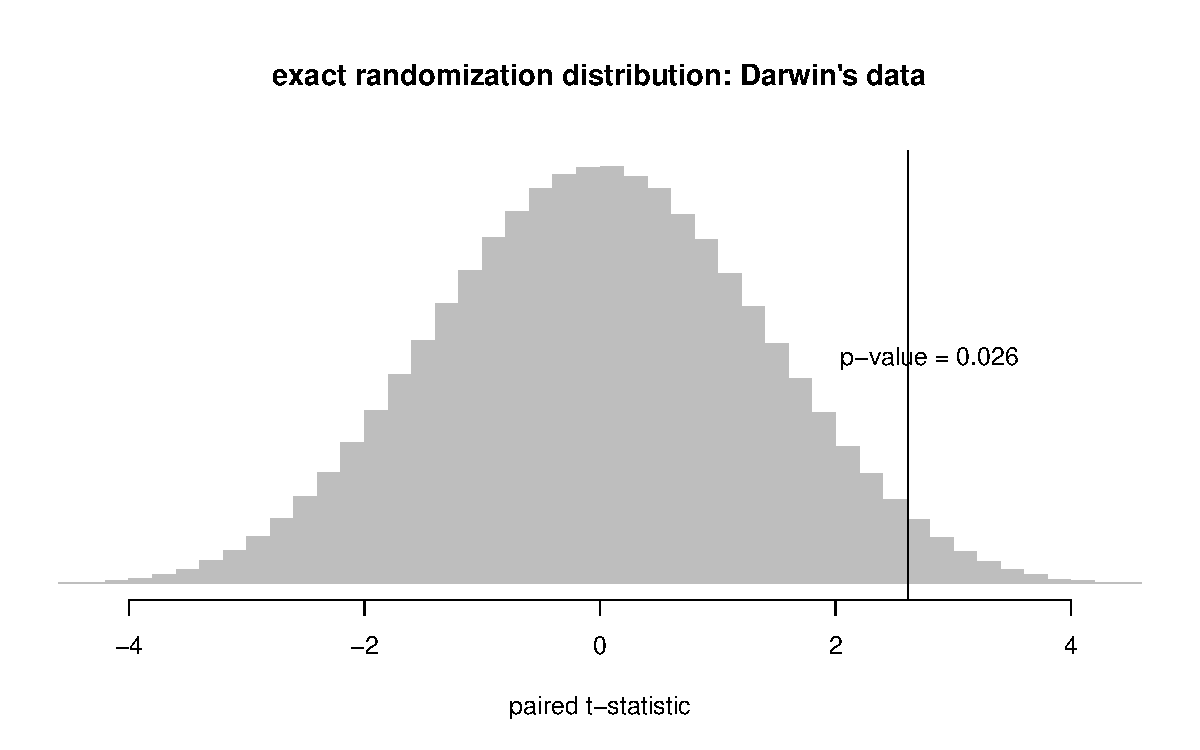
\includegraphics[width = \textwidth]{figures/frt_darwin.pdf}
\caption{利用 Darwin 数据得到的$\hat{\tau}$精确随机化分布}\label{fig::frt-darwin-mpe}
\end{figure}



\subsection{儿童电视教育实验数据}
\label{sec::neyman-television-mpe}



还重新分析了\citet{ball1973reading}中儿童电视工作坊实验的数据子集，\citet[][Chapter 10]{imbens2015causal}也分析过该数据。实验包含 8 对班级，每对随机选一个班，在正常阅读课时间观看{\it《电力公司》}节目。数据包含前测成绩（协变量）和后测成绩（结果）。下表汇总了对内协变量与结果及它们的差值：
\begin{lstlisting}
> dataxy = c(12.9, 12.0, 54.6, 60.6,
+            15.1, 12.3, 56.5, 55.5,
+            16.8, 17.2, 75.2, 84.8,
+            15.8, 18.9, 75.6, 101.9,
+            13.9, 15.3, 55.3, 70.6,
+            14.5, 16.6, 59.3, 78.4,
+            17.0, 16.0, 87.0, 84.2,
+            15.8, 20.1, 73.7, 108.6)
> dataxy = matrix(dataxy, 8, 4,  byrow = TRUE)           
> diffx = dataxy[, 2] - dataxy[, 1]
> diffy = dataxy[, 4] - dataxy[, 3]
> dataxy = cbind(dataxy, diffx, diffy)
> rownames(dataxy) = 1:8
> colnames(dataxy) = c("x.control", "x.treatment", 
+                      "y.control", "y.treatment",
+                      "diffx", "diffy")
> dataxy = as.data.frame(dataxy)
> dataxy
  x.control x.treatment y.control y.treatment diffx diffy
1      12.9        12.0      54.6        60.6  -0.9   6.0
2      15.1        12.3      56.5        55.5  -2.8  -1.0
3      16.8        17.2      75.2        84.8   0.4   9.6
4      15.8        18.9      75.6       101.9   3.1  26.3
5      13.9        15.3      55.3        70.6   1.4  15.3
6      14.5        16.6      59.3        78.4   2.1  19.1
7      17.0        16.0      87.0        84.2  -1.0  -2.8
8      15.8        20.1      73.7       108.6   4.3  34.9
\end{lstlisting}


下面的\ri{R}代码计算$\hat\tau$与$\hat V$。 
\begin{lstlisting}
> n      = dim(dataxy)[1]
> tauhat = mean(dataxy[, "diffy"])
> vhat   = var(dataxy[, "diffy"])/n
> tauhat
[1] 13.425
> sqrt(vhat)
[1] 4.636337
\end{lstlisting}
由命题\ref{prop::mpe-variance}和\ref{prop::colin2018regression}，可用 OLS 得到点估计与标准误。调整协变量后，有
\begin{lstlisting}
> unadj = summary(lm(diffy ~ 1, data = dataxy))$coef
> round(unadj, 3) 
            Estimate Std. Error t value Pr(>|t|)
(Intercept)   13.425      4.636   2.896    0.023
\end{lstlisting}
调整协变量后，有
\begin{lstlisting} 
> adj = summary(lm(diffy ~ diffx, data = dataxy))$coef
> round(adj, 3)
            Estimate Std. Error t value Pr(>|t|)
(Intercept)    8.994      1.410   6.381    0.001
diffx          5.371      0.599   8.964    0.000
\end{lstlisting}


这些结果要求$n$较大，只有认可大$n$近似，$p$值才有依据。但本例的$n=8$并不大，总共只有$2^8 = 256$种处理分配，所以最小可能$p$值是$1/256 = 0.0039$，远大于协变量调整估计量正态近似给出的$p$值。因此，更合理的做法是以学生化统计量——\ri{lm}函数给出的\ri{t value}——实施 FRT，计算精确$p$值。\footnote{其依据见第\ref{chapter::unification-fisher-neyman}章。}下面的\ri{R}代码计算基于两种$t$统计量的$p$值。 
\begin{lstlisting} 
> t.ran = sapply(1:2^8, function(x){ 
+   z.mpe = MP_enumerate(x, 8)
+   diffy.mpe = diffy*z.mpe
+   diffx.mpe = diffx*z.mpe
+   
+   c(summary(lm(diffy.mpe ~ 1))$coef[1, 3],
+     summary(lm(diffy.mpe ~ diffx.mpe))$coef[1, 3]) 
+ })
> p.unadj = mean(abs(t.ran[1, ]) >= abs(unadj[1, 3]))
> p.unadj
[1] 0.03125
> p.adj = mean(abs(t.ran[2, ]) >= abs(adj[1, 3]))
> p.adj
[1] 0.0078125
\end{lstlisting}


图\ref{fig::frt-television-mpe}给出了两个学生化统计量的精确分布及双侧$p$值。图中突出显示，检验统计量的随机化分布是离散的，至多只有 256 个取值。正态近似未必准确，尾部尤其如此，故应报告基于 FRT 的$p$值。 


\begin{figure}[th]
\centering
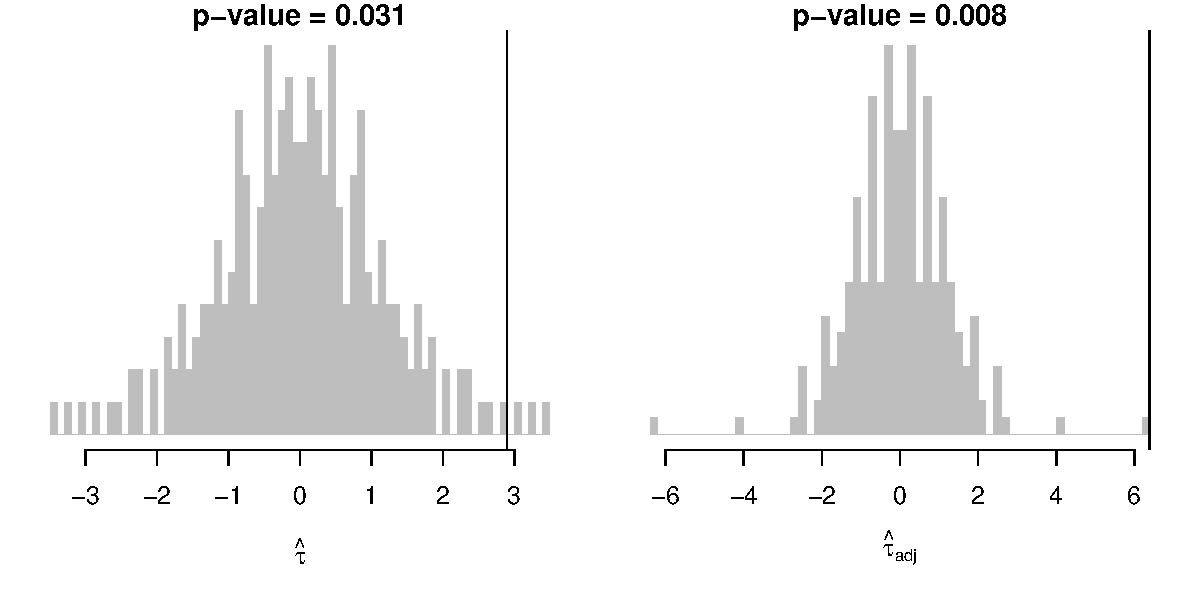
\includegraphics[width = \textwidth]{figures/frt_television.pdf}
\caption{第\ref{sec::neyman-television-mpe}节中学生化统计量的精确随机化分布}\label{fig::frt-television-mpe}
\end{figure}



\section{MPE与CRE的比较}
\label{sec::discussion}

\citet{imai2008variance}比较了配对实验与完全随机实验。直观上，若匹配良好且协变量能够预测结果，配对实验的估计更精确，但在设计阶段没有结果数据，难以判断这一条件是否满足。对于 FRT，若协变量能预测结果，配对实验通常比完全随机实验具有更高功效；\citet{greevy2004optimal}用基于 Wilcoxon 符号秩统计量的模拟说明了这一点。但有限样本下问题更微妙。考虑有$2n$个单位的实验，其中$n$个接受处理，$n$个作为对照。在$0.05$水平检验尖锐零假设时，配对实验至少需要$2\times 5=10$个单位，因为最小$p$值为$1/2^5 = 1/32 < 0.05$，但$1/2^4 = 1/16 > 0.05$；完全随机实验则至少需要$2\times 4 = 8$个单位，因为最小$p$值为$1/\binom{8}{4} = 1/70 < 0.05$，但$1/\binom{6}{3} = 1/20 = 0.05$。因此，只有$8$个单位时，配对实验不可能拒绝尖锐零假设，完全随机实验却有可能。即使协变量完美预测结果，按 FRT 衡量，配对实验也未必优于完全随机实验。 



\section{广义配对实验的推广}\label{sec::general-matched-experiment}

配对实验可直接推广为对照单位数可变的一般匹配实验。设有$n$个匹配集，编号为$i=1, \ldots, n$；第$i$个匹配集有$1+M_i$个单位，各$M_i$可以不同。实验总单位数为$N = n + \sum_{i=1}^n M_i$。用$ij$表示第$i$个匹配集中的第$j$个单位，其中$i=1,\ldots, n$、$j=1,\ldots, M_i+1$。单位$ij$的处理与对照潜在结果分别为$Y_{ij}(1)$和$Y_{ij}(0)$。 


在每个匹配集$i$中（$(i=1, \ldots, n)$），随机选且仅选一个单位接受处理，其余$M_i$个单位作为对照。这也是分层随机实验的特例：共有$n$层，各层大小为$1+M_i$，$(i=1, \ldots, n)$。令$Z_{ij}$为单位$ij$的处理指标，则观测结果为
$$
Y_{ij} = Z_{ij} Y_{ij}(1) + (1-Z_{ij}) Y_{ij}(0) . 
$$ 

匹配集$i$内的平均因果效应为
$$
\tau_i = (M_i + 1)^{-1} \sum_{j=1}^{1+M_i} \{ Y_{ij}(1)-Y_{ij}(0) \}. 
$$
由于一般匹配实验是分层随机实验，$\tau_i $的无偏估计量为
$$
\hat \tau_i = \sum_{j=1}^{M_i + 1} Z_{ij} Y_{ij} - M_i^{-1} \sum_{j=1}^{M_i+1} (1-Z_{ij}) Y_{ij}
$$
即匹配集$i$内的结果均值差。 

下面讨论一般匹配实验中的统计推断。 


\subsection{FRT}

同样，总可用 FRT 检验尖锐零假设
$$
\HF: Y_{ij}(1) = Y_{ij}(0)  \text{ for all }  i=1,\ldots, n; j=1,\ldots, M_i+1. 
$$
一般匹配实验是含许多小层的分层随机实验的特例，因此可使用例\ref{eg::hodgeslehmann}、\ref{eg::ks-stratified}、\ref{eg::mpe-sign-rank}、\ref{eg::mpe-ksstatistics}、\ref{eg::mpe-sign}的统计量，以及下面两小节的估计量及对应$t$统计量。 



\subsection{估计层内效应的平均值}


先考虑估计层内效应的平均值
$$
\tau = n^{-1} \sumn \tau_i .
$$
其无偏估计量为
$$
\hat\tau = n^{-1} \sumn \hat \tau_i . 
$$
有意思的是，定理\ref{thm::varianceest-mp}以及配对实验的其他结论仍适用于一般匹配实验。特别地，将各$\hat \tau_i $只对截距作 OLS 回归，就可得到$\tau$的点估计和方差估计。有协变量时，则将各$\hat \tau_i $对截距与各$\hat\tau_{X,i}$作 OLS 回归，其中
$$
\hat \tau_{X,i} = \sum_{j=1}^{M_i + 1} Z_{ij} X_{ij} - M_i^{-1} \sum_{j=1}^{M_i+1} (1-Z_{ij}) X_{ij}
$$
是匹配集$i$内相应的协变量均值差。 



\subsection{更一般的因果估计目标}


上面的$\tau$是各$\tau_i$的简单平均；各$M_i$不同时，它不等于实验中$N$个单位的平均因果效应。后者为
$$
\tau' = N^{-1} \sumn \sum_{j=1}^{1+M_i} \{ Y_{ij}(1)-Y_{ij}(0) \} = \sumn \frac{1+M_i}{N} \tau_i.
$$
为统一讨论，考虑加权因果效应
$$
\tau_w =  \sumn w_i \tau_i
$$
其中$\sumn w_i = 1$。它包括$w_i = n^{-1}$时的$\tau$，也包括对每个$i=1,\ldots, n$取$w_i = (1+M_i)/N $时的$\tau'$。容易得到无偏估计量
$$
\hat\tau_w =  \sumn w_i \hat\tau_i,
$$
及其方差
$$
\var(\hat\tau_w ) = \sumn w_i^2 \var (\hat\tau_i ). 
$$
但估计$\hat\tau_w $的方差相当棘手，因为各$\hat\tau_i$独立，却各自没有重复观测。这是\citet{hartley1969variance}和\citet{rao1970estimation}研究过的经典理论统计问题；\citet{fogarty2018mitigating}也讨论过，但未注意到这些早期工作。这里直接给出方差估计量，不详述构造动机：
$$
\hat{V}_w = \sumn c_i (\hat\tau_i -\hat\tau_w )  ^2
$$
其中
$$
c_i = \frac{    \frac{w_i^2}{1-2w_i}   }{   1 + \sumn  \frac{w_i^2}{1-2w_i} }.
$$
作为核查，配对实验中$M_i=1$且$w_i = n^{-1}$时，$c_i $简化为$ \{  n(n-1) \}^{-1}$。为简化讨论，假定对所有$i$均有$w_i < 1/2$，即没有任何匹配集占总权重的一半以上。下面的定理推广了定理\ref{thm::varianceest-mp}。  

\begin{theorem}
\label{thm::hadamdard-matched-experiment}
在各$M_i$可变的一般匹配实验中，若对所有$i$都有$w_i < 1/2$，则
$$
 E(\hat{V}_w ) - \var( \hat\tau_w  ) = \sumn c_i (\tau_i - \tau_w )^2 \geq \var( \hat\tau_w  )  \geq 0
 $$
各$\tau_i $相同时取等号。 
\end{theorem}

虽然$\hat{V}_w $的理论动机较复杂，直接验证定理\ref{thm::hadamdard-matched-experiment}却不太困难，证明留作习题\ref{para::variance-general-matched}。 
 



\section{作业习题}

\paragraph{MPE中$\hat{\tau}$的真实方差}
\label{para::variance-mp-design}

用潜在结果的有限总体方差表达$\var(\hat{\tau})$。 

\paragraph{协方差估计量的证明}\label{para::covariance-est-proof}
证明定理\ref{thm::covariance-mp}。

\paragraph{OLS方差估计方法}\label{para::seols-matchedpairs}
证明命题\ref{prop::mpe-variance}与\ref{prop::colin2018regression}。 


\paragraph{二元结果下的内曼推断}\label{para::binary-matchedpairs-neyman}


本题将例\ref{eg::mcnenar-test-binary}推广到 Neyman 推断。 

用表\ref{tb::binarymatchedpairs}中的计数表示$\hat\tau$与$\hat V$。 




\paragraph{最小样本量与FRT}
\label{prob::minimum-n-0.001}

推广第\ref{sec::discussion}节的讨论。考虑有$2n$个单位的实验，其中$n$个接受处理，$n$个作为对照，在$0.001$水平检验尖锐零假设。对于配对实验，要使最小$p$值不超过$0.001$，$n$至少应取多少？完全随机实验中相应的最小$n$是多少？
 

\paragraph{达尔文数据再分析}  
用威尔科克森统计量与内曼法重新分析该数据。

 
第\ref{sec::frt-darwin-mpe}节用统计量$\hat{\tau}$的 FRT 分析了 Darwin 数据。

改用 Wilcoxon 符号秩统计量的 FRT，重新分析该数据集。

采用 Neyman 推断重新分析该数据集，报告无偏点估计、保守方差估计及 95\% 置信区间。

\paragraph{电视实验数据再分析}  
对比不同检验法的结果差异。

第\ref{sec::neyman-television-mpe}节基于 Neyman 推断分析了这一数据集。

使用不同检验统计量的 FRT 重新分析该数据集。 

进行协变量调整，再用 FRT 重新分析该数据集。




\paragraph{重新分析\citet{angrist2009effects}的数据}\label{para::AL-mpe-neyman}

\citet{angrist2009effects}的原分析相当复杂。本题只关注原论文表 A1，并将学校视为实验单位。\citet{angrist2009effects}本质上对学校实施了配对实验。删除第 6 对及所有存在不依从的配对后，剩下 14 个完整配对，数据如下，也可从\ri{AL2009.csv}获得。 
\begin{lstlisting}
   pair z  pr99  pr00  pr01  pr02
1     1 0 0.046 0.000 0.091 0.185
2     1 1 0.036 0.051 0.000 0.047
3     2 0 0.054 0.094 0.184 0.034
4     2 1 0.050 0.108 0.110 0.095
5     3 0 0.114 0.000 0.056 0.075
6     3 1 0.098 0.054 0.030 0.068
7     4 0 0.148 0.162 0.082 0.075
8     4 1 0.134 0.390 0.339 0.458
9     5 0 0.152 0.105 0.083 0.129
10    5 1 0.145 0.077 0.579 0.167
11    6 0 0.188 0.214 0.375 0.545
12    6 1 0.179 0.165 0.483 0.444
13    7 0 0.193 0.771 0.328 0.583
14    7 1 0.189 0.186 0.168 0.368
15    8 0 0.197 0.350 0.000 0.383
16    8 1 0.200 0.071 0.667 0.429
17    9 0 0.213 0.176 0.164 0.172
18    9 1 0.209 0.165 0.092 0.151
19   10 0 0.211 0.667 0.250 0.617
20   10 1 0.219 0.250 0.500 0.350
21   11 0 0.219 0.153 0.185 0.219
22   11 1 0.224 0.363 0.372 0.342
23   12 0 0.255 0.226 0.213 0.327
24   12 1 0.257 0.098 0.107 0.095
25   13 0 0.261 0.071 0.000    NA
26   13 1 0.263 0.441 0.448 0.435
27   14 0 0.286 0.161 0.126 0.181
28   14 1 0.285 0.389 0.353 0.309
\end{lstlisting}
结果是 2001 年和 2002 年的 Bagrut 考试通过率，处理前协变量为 1999 年和 2000 年的通过率。分别进行调整与不调整协变量的 Neyman 推断，重新分析数据。特别地，如何处理第 25 对的缺失结果？ 
% (1) using the FRT with and without covariate adjustment and (2) based on the Neymanian inference with and without covariates. In particular, how do you deal with the missing outcome? 
 
 
\paragraph{广义配对实验的方差估计} 
 \label{para::variance-general-matched}

本题补充第\ref{sec::general-matched-experiment}节的细节。 
 
 
先证明一般匹配实验中的定理\ref{thm::varianceest-mp}，再证明定理\ref{thm::hadamdard-matched-experiment}。 
 
注：第二部分可先验证$\hat\tau_i -\hat\tau_w$的均值为$\tau_i - \tau_w$，方差为
$$
 \var(\hat\tau_i -\hat\tau_w) = \var(\hat\tau_w ) + (1-2w_i) \var(\hat\tau_i). 
 $$


\paragraph{推荐阅读}

\citet{greevy2004optimal}给出了基于协变量构造匹配对的算法。\citet{imai2008variance}讨论了不调整协变量时平均因果效应的估计，\citet{fogarty2018regression}讨论了配对实验中的协变量调整。 


  
 \chapter{随机实验中费希尔推断与内曼推断的统一}\label{chapter::unification-fisher-neyman}
 \chaptermark{费希尔推断与内曼推断的统一}


第\ref{ch::frt-cre}至\ref{chapter::mpe}章介绍了不同实验中的 Fisher 推断与 Neyman 推断。Fisher 视角检验任何单位都不存在因果效应的强零假设，关注有限样本精确$p$值；Neyman 视角关注平均因果效应的无偏估计及保守大样本置信区间。二者都由实验设计保证的实际随机化支持，因而都称为{\it 基于随机化的推断}或{\it 基于设计的推断}。由于讨论实验中有限总体的单位，也称为{\it 有限总体推断}。它们既相互联系，也各具特点。 

1935年，内曼向英国皇家统计学会提交了关于基于随机化推断的开创性论文。他的论文\citep{neyman1935statistical}在讨论环节遭到了费希尔的批驳。\cite{sabbaghi2014comments}回顾了这场著名的内曼-费希尔之争，并就该经典问题给出了新的研究结果。本章并不深究其中的哲学争议，而旨在提供一种统一的讨论框架。 



\section{在CRE中检验强零假设与弱零假设} 
 \label{sec::strong-weak-cre-frt}
 
 
重新考虑处理—对照完全随机实验。Fisher 视角检验强零假设
$$
\HF: Y_i(1) = Y_i(0) \text{ for all units } i=1,\ldots, n.
$$
FRT 给出\eqref{eq::exactpvalue}定义的有限样本精确$p_\frt$。 
 
 
由置信区间与假设检验的对偶性，Neyman 视角根据
$$
t= 
\frac{\hat{\tau} }{  \sqrt{  \hat{V}    } }  .
$$
检验弱零假设
$$
\HN : \tau = 0  \Longleftrightarrow \HN: \bar{Y}(1) = \bar{Y}(0)
$$
由$\hat\tau$的中心极限定理及方差估计的保守性，
$$
t  =   \sqrt{  \frac{ \var(\hat{\tau}) }{ \hat{V} } } \times  \frac{\hat{\tau} }{  \sqrt{  \var(\hat{\tau})   } }    \rightarrow  C \times   \N01 
$$
依分布收敛，其中$C$不大于$1$，但依赖未知潜在结果。将学生化统计量$t$与$\N01$的分位点比较，可得$\HN$的保守大样本检验。 

此外，\citet{ding2017randomization}证明：使用学生化统计量$t$开展FRT时具有双重保障：
\begin{enumerate}
\item 
 在强零假设$\HF$成立时，$p_\frt$值为有限样本精确值；
\item
 在弱零假设$\HN$成立时，$p_\frt$值具有大样本保守性。
\end{enumerate}
这种特性仅存在于学生化统计量$t$中。\citet{ding2017randomization}还指出：若采用其他统计量进行FRT，则未必能获得上述双重保障；特别是使用$\hat{\tau}$作为统计量时，在$\HN$成立条件下可能会出现大样本反保守性现象。以下我将通过理论分析阐释学生化操作在FRT中的必要性。 


在$\HN$下，有
$$
\hat{\tau} \asim \textsc{N}\left(0,    \frac{S^2(1)}{n_1} + \frac{S^2(0)}{n_0} -  \frac{S^2(\tau)}{n}    \right).
$$
FRT 假装科学表为$\HF$所规定的$(Y_i, Y_i)_{i=1}^n$，因此$\hat{\tau} $的随机化分布为
$$
(\hat{\tau} )^\pi \asim \textsc{N}\left(0,    \frac{s^2}{n_1} + \frac{s^2}{n_0}    \right),
$$
其中$(\cdot)^\pi$表示随机化分布。\footnote{$\pi$是表示随机置换的标准记号。}
$
s^2 
$
是观测结果的样本方差。根据第\ref{ch::frt-cre}章的\eqref{eq::frt-algebra-difference-in-means}，可将$\HF$下$(\hat{\tau} )^\pi$的渐近方差近似为
\begin{eqnarray*}
\frac{s^2}{n_1} + \frac{s^2}{n_0} 
& =& \frac{n}{n_1 n_0}  \left\{ 
 \frac{n_1 -1}{ n-1 } \hat S^2(1) + \frac{n_0 - 1}{n-1} \hat S^2(0) + \frac{n_1n_0}{n(n-1)} \hat\tau^2
 \right\} \\
&\approx & \frac{\hat S^2(1) }{n_0} +  \frac{\hat S^2(0) }{n_1} \\ 
&\approx & \frac{  S^2(1) }{n_0} +  \frac{  S^2(0) }{n_1},
\end{eqnarray*}
它不等于$\hat{\tau} $的渐近方差。理想情况下，检验$\HN$的$p$值应根据$\hat{\tau} $的真实分布计算，但它依赖未知潜在结果。FRT 则使用置换分布$(\hat{\tau} )^\pi $计算$p_\frt$，即使在大样本下也不等于$\HN$下$\hat{\tau} $的真实分布。因此，以$\hat\tau$作 FRT，即使大样本也未必控制$\HN$下的第一类错误率。 
 
 
幸运的是，将原统计量$\hat{\tau} $改为学生化版本$t$，就能消除以$\hat\tau$作 FRT 的上述问题。在$\HN$下，
$$
t \asim \textsc{N}(0,  C^2)
$$
其中$C^2 \leq 1$，且所有单位$i=1, \ldots, n$满足$Y_i(1) - Y_i(0) = \tau$时取等号。FRT 假装所有$i$都满足$Y_i(1) = Y_i(0) = Y_i$，生成置换分布
$$
t^\pi \asim \textsc{N}(0,  1)
$$
方差为$1$，因为 FRT 使用的科学表中个体因果效应均为零。在$\HN$下，$t$的真实分布比对应置换分布更集中，因此基于$t$的$p_\frt$渐近保守。 

%Whether $\HF$ or $\HN$ makes more sense? This is a famous controversy between Neyman and Fisher in a meeting at the Royal Statistical Society, UK \citep{neyman1935statistical, sabbaghi2014comments, Ding:2014}.  
%Recently, \citet{ding2017randomization} advocated using $\hat{\tau} /  \sqrt{  \hat{V}    } $, i.e., the studentized statistic $t$ in Example \ref{eg::studentized-statistic} of Chapter \ref{ch::frt-cre}, in the FRT so that the $p$-value is finite sample exact for $\HF$ and asymptotically valid for $\HN$.  In contrast, using the difference-in-means in the FRT does not have these guarantees. 







 
 
\section{CRE中的协变量校正型FRT}
 \label{sec::xfrt-cre}
 
将第\ref{sec::strong-weak-cre-frt}节推广到含协变量的情形，\citet{zhao2020caFRT}建议以学生化的\citet{lin2013}估计量进行 FRT：
$$
t_\textsc{L}   =  \frac{  \hat{\tau}_\textsc{L} }{  \sqrt{\hat{V}_\textsc{L}}  },
$$
它是将$Y_i$对$( 1, Z_i, X_i, Z_i X_i) $作 OLS 回归时，$Z_i$系数的稳健$t$统计量。他们证明，以$t_\textsc{L} $作 FRT 具有多重保证：
 \begin{enumerate}
\item
 在强零假设$\HF$条件下，$p_\frt$具有有限样本精确性；
\item
 在弱零假设$\HN$条件下，$p_\frt$具备大样本保守性；
\item
 当$\HN$不成立且协变量能预测结果时，$p_\frt$对应检验的渐近功效高于基于$t$的 FRT；
\item
即便线性结果模型设定存在偏差，上述特性依然成立。 
\end{enumerate}
这同样是学生化统计量$t_\textsc{L} $的特性。\citet{zhao2020caFRT}证明，第\ref{sec::covariate-adjusted-frt-intro}节的其他协变量调整 FRT，可能在$\HN$下反保守，或在$\HN$不成立时功效低于基于$t_\textsc{L} $的 FRT。  




\section{模拟研究}
\label{sec::simulation-xfrt-typeoneerror}




下面通过模拟评价弱零假设下各$p_\frt$的有限样本性质，使用以下十二种统计量。
\begin{enumerate}
\item
前三种统计量源自内曼\citet{Neyman:1923}的OLS推导，依次为处理组系数、基于经典标准误的$t$统计量及基于EHW标准误的$t$统计量。

\item
接下来三个统计量采用定义\ref{def::pseudo-y-frt}的伪结果策略，\citet{rosenbaum2002covariance}倡导过该方法。先将$Y_i$对$(1,X_i)$回归，得到残差，再像前三个统计量一样构造统计量。

\item
接下来三个统计量基于\citet{fisher1925statistical}的 OLS 实现，见第\ref{sec::ancova}节。

\item
最后三种对应\citet{lin2013}的OLS推导，亦在第\ref{sec::ancova}章中探讨。
\end{enumerate}

 


考虑包含$n=100$个单位的有限总体，实施组别大小为$(n_1, n_0) =(20,80)$的完全随机实验。对每个$i  $，从 Unif$(-1,1)$抽取一元协变量$ X_i $，生成潜在结果$Y_i(1) \sim \textsc{N}(  X_i ^3 , 1)$和$Y_i(0) \sim \textsc{N}( - X_i ^3 , 0.5^2)$，再分别中心化各$Y_i(1)$与$Y_i(0)$，保证$\tau= 0$。模拟时固定$\{Y_i(1), Y_i(0),  X_i \}_{ i = 1}^{n} $，随机置换$n_1$个 1 与$n_0$个 0，得到观测结果并实施 FRT。重复 500 次，每次用处理向量的 500 次独立置换近似$p$值。 



图\ref{fig::xfrt-type1error}呈现了弱零假设下的$p$值分布。唯独底部四列稳健$t$统计量能维持第一类错误率在设定水平，且呈保守特性符合理论预期。其余八种统计量均导致第一类错误率超出名义水平，故不宜用于弱零假设检验。

 



\begin{sidewaysfigure} 
\centering
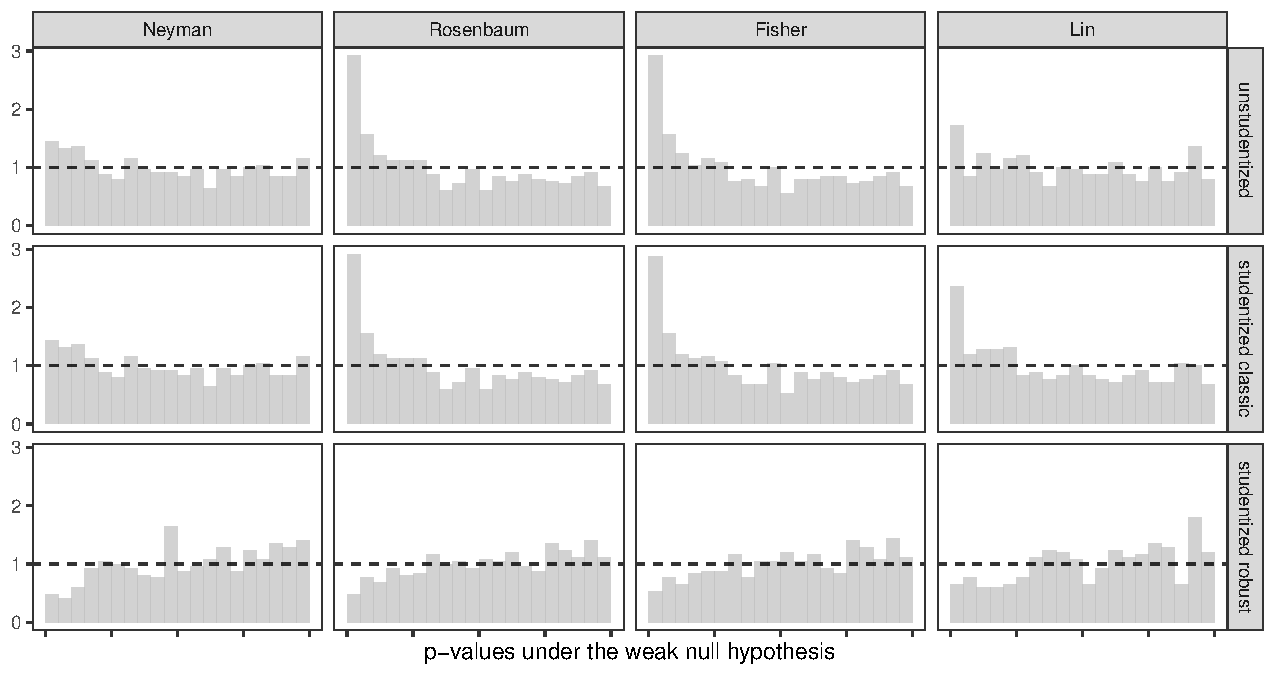
\includegraphics[width = \textwidth]{figures/typeoneerrorXFRT.pdf}
\caption{弱零假设下$p_\frt$值的直方图}\label{fig::xfrt-type1error}
\end{sidewaysfigure}










\section{综合建议}






若需同时检验强弱零假设，SRE场景下的建议与CRE相似。回顾第\ref{chapter::stratification-poststratification}章与\ref{sec::covariate-SRE}章的估计量：无协变量时\citet{zhao2020caFRT}推荐采用
$$
t_\textsc{S} =  \frac{  \hat{\tau}_\textsc{S} }{  \sqrt{\hat{V}_\textsc{S}} } ;
$$ 
存在协变量时则建议利用
$$
t_\textsc{L,S} =  \frac{  \hat{\tau}_\textsc{L,S} }{  \sqrt{\hat{V}_\textsc{L,S}} } . 
$$ 


再随机化的分析更微妙。\citet{zhao2020caFRT}证明，基于$t$的 FRT 不再具有第\ref{sec::strong-weak-cre-frt}节的双重保证，但基于$t_\textsc{L}$的 FRT 仍保有第\ref{sec::xfrt-cre}节的保证，说明再随机化下协变量调整与学生化都很重要。 




配对实验也有类似结论。不含协变量时，建议将$\hat\tau_i$仅对$1$作 OLS 回归，以截距的$t$统计量实施 FRT；含协变量时，将$\hat\tau_i$对$1$与$\hat\tau_{X,i}$回归，以截距的$t$统计量实施 FRT。第\ref{chapter::mpe}章图\ref{fig::frt-television-mpe}采用了这些推荐方法。 



总体上，以学生化统计量实施 FRT 是更稳妥的选择。若学生化统计量的大样本正态近似准确，$p_\frt$与正态近似$p$值几乎相同；若近似不准确，FRT 至少仍保证强零假设下$p$值有效。这就是本书的建议。 



\section{案例研究}
\label{sec::case-study-chong}

 

回顾第\ref{sec::ps-chong}节分析的\citet{chong2016iron}分层随机实验，分别比较“足球”组与“对照”组、“医生”组与“对照”组，并比较是否使用基线贫血状态协变量的 FRT。该数据可同时说明完全随机实验和分层随机实验的 FRT：同一年级内的十项亚组分析使用完全随机实验的$t$和$t_\textsc{L}$；对所有年级平均的两项总体分析使用分层随机实验的$t_\textsc{S}$和$t_\textsc{L,S}$。 

表\ref{tb::pv-values-chong}给出点估计、标准误、稳健$t$统计量正态近似的$p$值，以及 FRT 的$p$值。由于基线贫血能预测结果，多数层中协变量调整降低了标准误。表\ref{tb::pv-values-chong}也有两个例外：二年级比较“足球”与“对照”、四年级比较“医生”与“对照”时，调整后标准误增加。这是层内组别人数较少、渐近近似不准确所致，但两例的差异都仅在第三位数字。正态近似与 FRT 的$p$值很接近，后者多数略大。根据理论，应更信赖 FRT 的$p$值，因为它还有尖锐零假设下有限样本精确的额外保证。本例层内人数很少，这一点尤其重要。 

\begin{table}
\centering
\caption{基于\citet{chong2016iron}数据的再分析：“\textsc{N}”表示\citet{Neyman:1923}的不调整协变量估计与检验，“\textsc{L}”表示\citet{lin2013}的协变量调整估计与检验。}\label{tb::pv-values-chong}
\begin{subtable}[h]{0.45\textwidth}
\caption{足球组 vs 对照组}
    \begin{tabular}{rrrrr}
    \hline 
   &    估计值 & 标准误 &$p_\text{Normal}$ & $p_\frt$ \\
       类别1& &&&\\
\textsc{N}  &  0.051 &0.502 &     0.919  & 0.924 \\
\textsc{L}   &    0.050 & 0.489 &     0.919 &  0.929 \\
       类别2& &&&\\
\textsc{N}  &  -0.158 &0.451  &    0.726  & 0.722\\
\textsc{L}   &  -0.176 & 0.452   &   0.698  & 0.700 \\
       类别3& &&&\\
\textsc{N}  &  0.005 &0.403  &    0.990 &  0.989 \\
\textsc{L}   &   -0.096& 0.385 &     0.803&   0.806 \\
       类别4& &&&\\
\textsc{N}  &  -0.492& 0.447  &    0.271 &  0.288 \\
\textsc{L}   &    -0.511& 0.447  &    0.253 &  0.283 \\
       类别5& &&&\\
\textsc{N}  &  0.390& 0.369 &     0.291 &  0.314 \\
\textsc{L}   &   0.443 &0.318  &    0.164  & 0.186 \\
       全部& &&&\\
\textsc{N}  &  -0.051 & 0.204  &    0.802 &  0.800 \\
\textsc{L}   &    -0.074& 0.200   &   0.712  & 0.712\\
\hline 
    \end{tabular}
\end{subtable}

\begin{subtable}[h]{0.45\textwidth} 
\caption{医生组 vs 对照组}
    \begin{tabular}{rrrrr}
    \hline 
   &    估计值 & 标准误 &$p_\text{Normal}$ & $p_\frt$ \\
       类别1& &&&\\
\textsc{N}  &  0.567 &0.426  &    0.183 &  0.192 \\
\textsc{L}   &   0.588& 0.418  &   0.160  & 0.174 \\
       类别2& &&&\\
\textsc{N}  &   0.193& 0.438 &     0.659 &  0.666 \\
\textsc{L}   &  0.265& 0.409   &   0.517  & 0.523 \\
       类别3& &&&\\
\textsc{N}  &  1.305& 0.494  &    0.008 &  0.012\\
\textsc{L}   &  1.501& 0.462   &   0.001  & 0.003 \\
       类别4& &&&\\
\textsc{N}  &  -0.273& 0.413  &    0.508 &  0.515 \\
\textsc{L}   &  -0.313& 0.417   &   0.454  & 0.462\\
       类别5& &&&\\
\textsc{N}  & -0.050 &0.379  &    0.895 &  0.912 \\
\textsc{L}   &  -0.067& 0.279  &    0.811 &  0.816 \\
       全部& &&&\\
\textsc{N}  &  0.406 & 0.202   &   0.045 &  0.047\\
\textsc{L}   &    0.463 & 0.190   &   0.015  & 0.017 \\
\hline 
    \end{tabular}
\end{subtable}
\end{table}



图\ref{fig::randomization-distributions-chong}比较了稳健$t$统计量随机化分布的直方图与渐近近似。亚组分析中，随机化分布与$\textsc{N}(0,1)$有可见差异；对各年级平均后，差异几乎消失。本例正态近似$p$值与 FRT 相差不大，两者结论一致：由医生说明铁剂益处的视频提高了学业表现，三年级学生中的效应最显著；由知名足球运动员说明铁剂益处的视频则没有显著效应。 



\begin{sidewaysfigure}
\centering
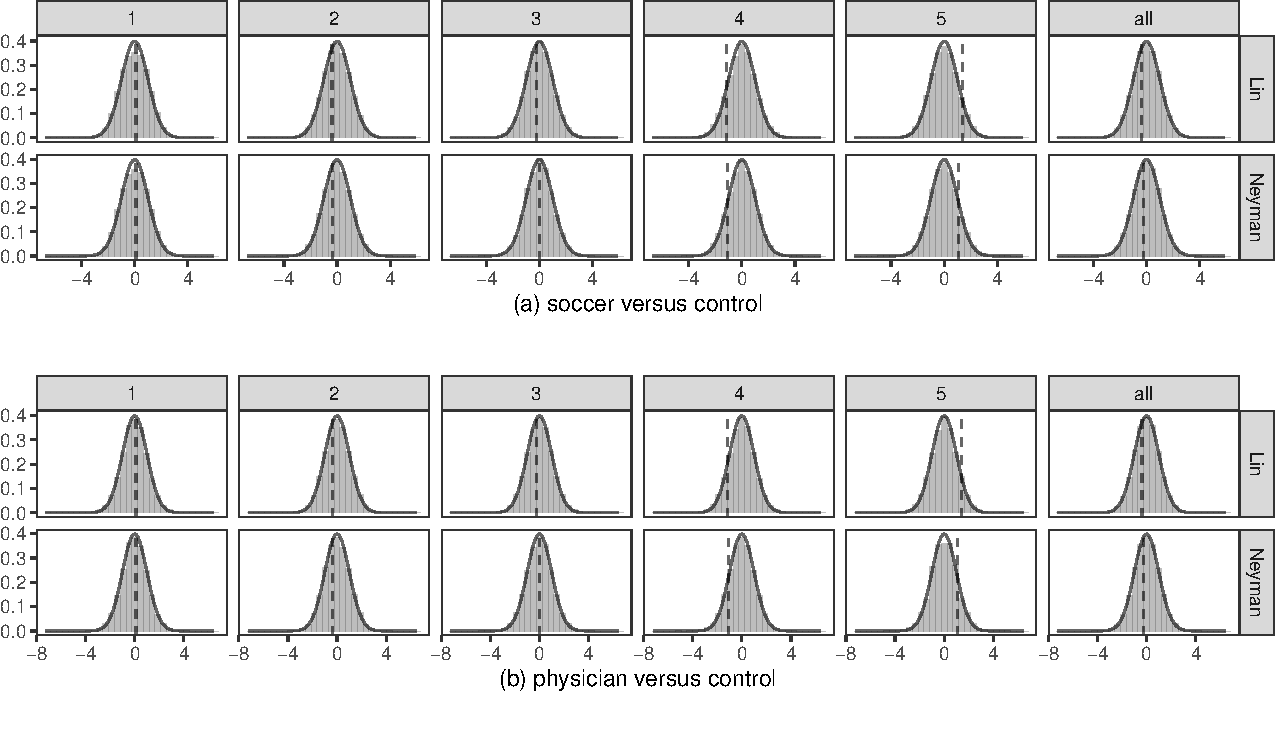
\includegraphics[width = \textwidth]{figures/frt_dist_chong.pdf}
\caption{\citet{chong2016iron}数据的再分析：含$5\times 10^4$次蒙特卡洛抽样的结果分布与$\N01$近似}
\label{fig::randomization-distributions-chong}
\end{sidewaysfigure}


 \section{作业习题}


\paragraph{重新分析\citet{angrist2009effects}的数据}\label{para::AL-mpe-fisher}

本题为内曼视角下的对应习题\ref{para::AL-mpe-neyman}。请计算各类学生化统计量对应的$p_\frt$值。 


\paragraph{复现\citet{zhao2020caFRT}的图1}\label{para::zhaoding-xfrt}

\citet{zhao2020caFRT}模拟比较不同统计量 FRT 的$p_\frt$有限样本性质，并根据图 1 推荐用$t_\textsc{L,S} $的 FRT 分析分层随机实验。请复现其图 1。 


\paragraph{推荐阅读}

在置换检验中使用学生化统计量并非新想法，参见\citet{Janssen97}和\citet{Romano13}。在基于设计的框架下，\citet{ding2017randomization}和\citet{wu2018randomization}针对多处理组实验提出了这一建议，\citet{zhao2020caFRT}将其推广到协变量调整。  

   
    \chapter{有限总体与超总体因果推断的衔接}\label{chapter::bridging}
 \chaptermark{有限总体与超总体因果推断的衔接}


 


我们之前重点讨论了随机实验中的有限总体视角。该视角将所有潜在结果视为固定数值。即便这些潜在结果本质上是随机变量，在有限总体视角下我们仍能将其视为已知条件。这种视角的优势在于：
\begin{enumerate}
\item
它侧重于实验设计本身；
\item
它对结果生成过程所需的假设条件极少。
\end{enumerate}
然而，这种视角常受到批评，被认为仅具备{\it 内部有效性}，未必具备{\it 外部有效性}。两者的非正式定义如下。 

\begin{definition}
[内部有效性]
统计分析结果对当前研究样本有效。 
\end{definition}


\begin{definition}
[外部有效性]
统计分析结果对超出研究样本范围的更大总体也有效。 
\end{definition}



显然，所有实验者都希望自己的实验结果既具备内部有效性又具备外部有效性。由于在有限总体视角下所有统计性质均以现有样本的潜在结果为前提，因此相关结论仅适用于这些观测对象。此时一个自然的问题便浮现出来：有限总体视角下的结论能否推广到更大总体呢？ 



从潜在结果角度出发，有限总体框架确实存在这样的局限性。不过这也可视为一个哲学层面上的问题。我们所观测到的毕竟是有限总体，任何实验设计与分析所提供的信息均针对这一有限总体。随机化机制仅能在给定个体潜在结果的条件下确保内部有效性。至于结果的外部有效性，则取决于这些个体的抽样方式。倘若该有限总体恰是我们所关心的更大总体的代表性样本，那么实验结果自然也具备外部有效性；反之，基于随机化推断得出的结论则可能不具备推广性。为严谨探讨此问题，我们需要一个包含双重随机性的框架：其一是个体的抽样随机性，其二是干预措施分配的随机性。关于此点的正式探讨可参见\citet{miratrix2018worth}与\citet{abadie2020sampling}的论述。\footnote{\citet{pearl2014external}则从因果图的角度探讨了{\it 可迁移性}问题。}
  
  
  
  
对某些统计学家而言，这只是个技术性问题。我们可修改统计框架，假定个体是从超总体中抽样而得。如此一来所有结论便都关于所关注的总体了。这个框架虽看似便捷，却并未真正解决前述问题。下文我将介绍该框架，主要出于两个目的：
\begin{enumerate}
\item
它为随机实验提供了另一种视角；
\item
它充当了本书\ref{part::rcts}与\ref{part::observational-studies}两大部分之间的桥梁。
\end{enumerate}
后者尤为重要，因为超总体框架能帮助我们针对干预措施非随机分配的观测性研究得出更有价值的结论。 





\section{CRE}\label{sec::cre-superpop}

假设从某个超总体中抽样得到
$$
\{  Z_i, Y_i(1), Y_i(0),  X_i  \}_{i=1}^n  \iidsim \{  Z, Y(1), Y(0), X \}
$$
因此我们可以省略该总体中各量的下标 $i$。稍作记号约定后，我们将总体平均因果效应定义为
$$
\tau  = E\{  Y(1)  - Y(0)\}  = E\{  Y(1)  \} -  E\{ Y(0)\} .
$$
在超总体框架下，CRE可表述如下。

\begin{definition}
[超总体框架下的CRE]
\label{def::cre-superpopulation}
此时有
$$
Z \ind \{  Y(1), Y(0), X \} .
$$
\end{definition}

依据定义\ref{def::cre-superpopulation}，平均因果效应可表示为
\begin{eqnarray}
\tau &=& E\{  Y(1) \mid Z=1\}  - E\{  Y(0) \mid Z=0 \}   \nonumber  \\
&=& E( Y \mid Z=1)  - E(  Y \mid Z=0 ),
\label{eq::cre-identifiable}
\end{eqnarray}
即两个条件下结果期望值的差值。公式\eqref{eq::cre-identifiable}的第一行正是利用随机化机制的关键步骤。由于 $\tau  $ 可由观测变量的分布直接导出，因此它属于{\it 非参数可识别}\footnote{在因果推断中，若仅依据观测变量分布即可确定某参数而无需额外参数假设，则称该参数具有非参数可识别性。更正式的讨论见后文定义\ref{def::nonparametric-identification}。}。公式\eqref{eq::cre-identifiable}直接提示了矩估计量 $\hat{\tau}$ 的存在形式——即前述结果均值之差。以 $\bm{Z}$ 为条件后，此即典型的双样本均值比较问题。此时有
$$
E(  \hat{\tau} \mid \bm{Z}) = \tau
$$
以及
$$
\var (  \hat{\tau} \mid \bm{Z}) =   \frac{ \var\{ Y(1) \}}{n_1} + \frac{ \var\{ Y(0) \}}{n_0}.
$$
在独立同分布抽样条件下，样本方差是总体方差的无偏估计，因此\citet{Neyman:1923}提出的方差估计器也同样是 $\var (  \hat{\tau} \mid \bm{Z}) $ 的无偏估计。超总体框架下此保守性问题便不复存在。


我们亦可探讨协变量调整法。基于OLS分解式（参见章节\ref{appendix::basic-linear-regression}）
\begin{eqnarray}
Y(1) &=& \gamma_1 + \beta_1\tran X + \varepsilon(1),\label{eq::ols-decomposition-y1}\\
Y(0) &=& \gamma_0 + \beta_0\tran X + \varepsilon(0),\label{eq::ols-decomposition-y0}
\end{eqnarray}
可得
\begin{eqnarray*}
\tau  &=& E\{  Y(1)  - Y(0)\} \\
&=& \gamma_1  -  \gamma_0 + (\beta_1 - \beta_0)\tran E(X),
\end{eqnarray*}
此处因截距项的引入，残差 $  \varepsilon(1)$ 与 $\varepsilon(0)$ 的期望值均为零。我们可分别对处理组与对照组数据实施OLS回归以估计\eqref{eq::ols-decomposition-y1}与\eqref{eq::ols-decomposition-y0}中的系数。设其样本估计量依次为 $\hat{\gamma}_1, \hat{\beta}_1, \hat{\gamma}_0, \hat{\beta}_0$，则经协变量调整后的 $\tau $ 估计量为
$$
\hat{\tau}_\text{adj} =  \hat \gamma_1  - \hat  \gamma_0 + (\hat \beta_1 - \hat \beta_0)\tran \bar{X}.
$$
若将协变量中心化处理使 $ \bar{X} = 0$，则上述估计量便等同于\citet{lin2013}提出的估计器
$$
\hat{\tau}_\textsc{L} = \hat \gamma_1  - \hat  \gamma_0,
$$
此值恰为含处理组-协变量交互项的合并回归中 $Z$ 的系数；参见命题\ref{prop::lin-ols}。 



遗憾的是，在超总体框架下，协变量样本均值$\bar{X} $还具有额外的不确定性，因此 EHW 方差估计量不适用于$\hat{\tau}_\textsc{L}$。\citet{berk2013covariance}、\citet{negi2020revisiting}和\citet{zhao2020caFRT}提出在 EHW 方差估计量中加入修正项
\begin{equation}\label{eq::lin-ehw-correction}
(\hat \beta_1 - \hat \beta_0)\tran S_X^2  (\hat \beta_1 - \hat \beta_0)  / n
\end{equation}
其中，$\hat \beta_1 - \hat \beta_0$是在计算\citet{lin2013}的估计量时交互项$Z_iX_i$的系数，$S_X^2$是协变量的有限总体协方差矩阵。一种概念上更简单、但计算量更大的办法是用自助法估计方差；参见第\ref{sec::bootstrap}节和习题\ref{hw::variance-bootstrap-superpopulation}。 



\section{基于CRE的超总体视角模拟实验}
\label{sec::simulation-CRE-superp}


下述\ri{linestimator}函数可计算超总体情形下的\citet{lin2013}估计量、EHW标准误以及基于\eqref{eq::lin-ehw-correction}的修正标准误。 
\begin{lstlisting}
library("car")
linestimator = function(Z, Y, X){
  ## standardize X
  X      = scale(X)
  n      = dim(X)[1]
  p      = dim(X)[2]
  
  ## fully interacted OLS
  linreg = lm(Y ~ Z*X)
  est    = coef(linreg)[2]
  vehw   = hccm(linreg)[2, 2]
  
  ## super population correction
  inter  = coef(linreg)[(p+3):(2*p+2)]
  vsuper = vehw + sum(inter*(cov(X)%*%inter))/n
  
  c(est, sqrt(vehw), sqrt(vsuper))
}
\end{lstlisting}


下面通过模拟比较 EHW 标准误与修正后的标准误。样本量取$n=500$，进行 2000 次蒙特卡洛重复。潜在结果是协变量的非线性函数，误差项也不服从正态分布。真实平均因果效应为$0.$。
\begin{lstlisting}
res = replicate(2000, {
  n  = 500
  X  = matrix(rnorm(n*2), n, 2)
  Y1 = X[, 1] + X[, 1]^2 + runif(n, -0.5, 0.5)
  Y0 = X[, 2] + X[, 2]^2 + runif(n, -1, 1)
  Z  = rbinom(n, 1, 0.6)
  Y  = Z*Y1 + (1-Z)*Y0
  linestimator(Z, Y, X)
})
\end{lstlisting}


模拟结果完全印证了理论推测。首先，\citet{lin2013}估计量近乎无偏。其次，EHW标准误均值小于经验标准差，致使95\% 置信区间覆盖率不足。最后，经修正的超总体标准误均值与经验标准差高度吻合，从而准确实现了95\% 置信区间的覆盖率控制。  
\begin{lstlisting}
> ## bias
> mean(res[1, ])
[1] -0.0001247585
> ## empirical standard deviation
> sd(res[1, ])
[1] 0.1507773
> ## estimated EHW standard error
> mean(res[2, ])
[1] 0.1388657
> ## coverage based on EHW standard error
> mean((res[1, ]-1.96*res[2, ])*(res[1, ]+1.96*res[2, ])<=0)
[1] 0.927
> ## estimated super population standard error
> mean(res[3, ])
[1] 0.1531519
> ## coverage based on population standard error
> mean((res[1, ]-1.96*res[3, ])*(res[1, ]+1.96*res[3, ])<=0)
[1] 0.9525
\end{lstlisting}

\section{推广到分层随机实验}

第\ref{sec::cre-superpop}节的讨论可以推广到分层随机实验，因为它等价于各层内相互独立的完全随机实验。 
%The discussion will also extend to the MPE since it is a special case of the SRE. 
下面的记号与第\ref{chapter::stratification-poststratification}章略有不同。 


设
$$
\{ Z_i,  Y_i(1), Y_i(0) ,  X_i  \}  \iidsim \{ Z,  Y(1), Y(0), X  \} .
$$ 
设定离散型协变量 $ X_i \in \{ 1,\ldots, K\}$，此时SRE可表述如下。


\begin{definition}
[超总体框架下的SRE]\label{def::sre-superpopulation}
此时有
$$
Z\ind\{  Y(1), Y(0) \} \mid   X  .
$$
\end{definition}


依定义\ref{def::sre-superpopulation}，条件平均因果效应可改写为
\begin{eqnarray*}
\tau_{[k]}  &=&  E\{   Y(1) -  Y(0)  \mid X= k \} \\
&=& E(Y\mid Z=1, X=k) - E(Y\mid Z=0, X=k),
\end{eqnarray*}
进而总体平均因果效应可表示为
\begin{eqnarray*}
\tau &=&   E\{   Y(1) -  Y(0)   \}  \\
&=& \sum_{k=1}^K \pr(X = k) E\{   Y(1) -  Y(0)  \mid X = k \} \\
&=& \sum_{k=1}^K \pr(X  = k) \tau_{[k]} .
\end{eqnarray*}
%
% The covariates $ X_i $'s are fixed with marginal proportions $\pi_{[k]} = \#\{ i:  X_i  = k \} / n$ for  $k=1,\ldots, K$. 
%The MPE corresponds to the case in which $K=n/2$ and there is only one treated and one control unit with $ X_i  = k$ for all $k=1,\ldots, K$. 
%The stratum-specific average causal effect is
%$$
%\tau_{[k]} = E\{  Y_{[k]}(1) -  Y_{[k]}(0) \} ,
%$$
%and the population average causal effect is
%$$
%\tau  = \sum_{k=1}^K \pi_{[k]} \tau_{[k]} .
%$$
第\ref{sec::cre-superpop}节的讨论在每一层内都成立，因此可以推导出分层随机实验在超总体框架下的对应结论。若每一层的处理单位和对照单位均多于两个，就可以用$\hat{V}_\textsc{S}$作为$\var( \hat{\tau}_\textsc{S} )$的方差估计量。 


%Unsurprisingly, the MPE is more subtle since $\hat{V}_\textsc{S}$ is not well defined. With $\{\hat{\tau}_{[1]} , \ldots, \hat{\tau}_{[n/2]} \}$, we can use  
%$$
%\hat{V} = \frac{1}{  n/2(n/2-1) } \sum_{k=1}^{n/2} (  \hat{\tau}_{[k]} -  \hat{\tau}_\textsc{S})^2
%$$
%to estimate the variance of $\hat{\tau}_\textsc{S}$. Similar to our proof before, we can show that 
%\begin{eqnarray}
%\label{eq::super-pop-mpe-var}
%E(\hat{V}) - \var( \hat{\tau}_\textsc{S} ) =  \frac{1}{  n/2(n/2-1) } \sum_{k=1}^{n/2} ( \tau_{[k]} -  \tau)^2 \geq 0,
%\end{eqnarray}
%so $\hat{V} $ is still a conservative variance estimator. Unlike the CRE and SRE, the conservativeness issue does not go away for the MPE even under the superpopulation framework. 
%  
%  
%Sometimes, we may further assume that the covariates are random draws in the SRE and MPE:
%$$
%\{Z_i,  Y_i(1), Y_i(0) ,  X_i    \}  \iidsim \{   Z_i,  Y_i(1), Y_i(0) ,  X_i   \}
%$$
%with
%$$
%Z \ind\{  Y(1), Y(0) \} \mid  x  .
%$$
%The population average causal effect simplifies to
%$$
%\tau  = E\{  Y(1) -  Y(0) \}
%=\sum_{k=1}^K  E\{  Y(1) -  Y(0) \mid x = k \} \pr(x  = k).
%$$
%The estimators remain unchanged. This framework brings mathematical convenience due to the IID assumption. However, it seems especially awkward in the MPE when the pair indicators are IID which invalidates the motivation for the experimental design itself. We should impose IID assumptions with caution. 


后文第\ref{part::observational-studies}部分将给出定义\ref{def::sre-superpopulation}的具体形式。 
  

 \section{作业习题}
 
\paragraph{完全随机实验中观测结果的 OLS 分解}\label{hw::ols-decompose-cre}

依据\eqref{eq::ols-decomposition-y1}与\eqref{eq::ols-decomposition-y0}，试证观测结果可分解为如下形式
$$
Y= \alpha_0 + \alpha_Z  Z +
\alpha_X \tran X + \alpha_{ZX} \tran X Z + \varepsilon 
$$
其中系数关系为
$$
\alpha_0 = \gamma_0 ,\quad
\alpha_Z = \gamma_1 - \gamma_0,\quad
\alpha_X  =  \beta_0, \quad
\alpha_{ZX} = \beta_1 - \beta_0
$$
且残差项可表为
$$
\varepsilon  = Z \varepsilon (1) + (1-Z) \varepsilon (0). 
$$
换言之，
$$
(\alpha_0, \alpha_Z, \alpha_X , \alpha_{ZX} )
=\arg\min_{a_0, a_Z, a_X, a_{ZX}   }  E  (  Y - a_0 - a_Z Z - a_X\tran X -a_{ZX} \tran X Z)^2.
$$ 
 
 
\paragraph{超总体框架下\citet{lin2013}估计量的方差估计}\label{hw::variance-bootstrap-superpopulation}
 
在超总体框架下，根据\eqref{eq::ols-decomposition-y1}和\eqref{eq::ols-decomposition-y0}生成模拟数据$\{  X_i, Z_i, Y_i(1), Y_i(0) \}_{i=1}^n$，并令$\beta_1 \neq \beta_0$成立。在每个模拟数据集中计算\citet{lin2013}的估计量，比较真实方差与下列方差估计值：
\begin{enumerate}
\item
EHW稳健型方差估计值；
\item
含修正项\eqref{eq::lin-ehw-correction}的改进型EHW方差估计值；
\item
协变量初始中心化处理且每次自助法抽样不再重新调整的Bootstrap方差估计值；
\item
每次自助法抽样前均重新中心化协变量的Bootstrap方差估计值。
\end{enumerate}

  
 
% \paragraph{Variance estimation in the MPE}
% Show \eqref{eq::super-pop-mpe-var} under the super population framework. 


\paragraph{推荐阅读}


\citet{ding2017bridging}系统探讨了有限总体与超总体两种情境下平均因果效应的推断方法。 

  
   
   
 
\part{观察性研究}\label{part::observational-studies}
  \chapter{观察性研究、选择偏差与因果效应的非参数识别}\label{chapter::observational-studies}
 \chaptermark{观察性研究}

 
\citet{cochran1965planning}总结了观察性研究的两个共同特征：
\begin{enumerate}
\item
目标是阐明因果关系；
\item 
无法通过控制实验来实现研究目的。 
\end{enumerate}

第一个特征与本书第\ref{part::rcts}部分讨论的随机实验相同，但第二个特征与随机实验存在本质区别。 


\citet{dorn1953philosophy}指出，观察性研究的设计者应当时刻思考以下问题：
\begin{quote}
如果能够通过控制实验完成研究，那么实验过程会是怎样的？
\end{quote}
遵循\citet{dorn1953philosophy}的建议总是有益的，因为潜在结果框架与实验存在内在联系——无论是真实实验还是思想实验。本书第\ref{part::observational-studies}部分将探讨基于观察性研究的因果推断，阐明其与随机实验的根本差异。不过许多基于观察性研究的因果推断思想同样与随机实验密切相关。 

 


\section{示例说明}
 
 \begin{example}
 [职业培训项目]\label{eg::job-training-obs}
 \citet{lalonde1986evaluating}研究职业培训项目对收入的因果效应，比较随机实验与观察性研究的结果。此前已使用过实验数据，即\ri{Matching}包中的\ri{lalonde}；也在第\ref{section:correlatioandregressionintro}节和习题\ref{hw::lalonde-obs-reg}中使用过观察性对应数据\ri{cps1re74.csv}。\citet{lalonde1986evaluating}发现，许多传统统计或计量经济学方法在观察性数据上得到的估计，与实验估计相差很大。\cite{dehejia1999causal}采用因果推断启发的方法重新分析，发现能较好地恢复实验这一金标准。此后，这成为观察性研究因果推断中的经典例子。 
 \end{example}
 
 
  \begin{example}
 [吸烟与同型半胱氨酸]\label{eg::nhanes2005-2006}
 \citet{bazzano2003relationship}利用2005–2006年美国国家健康与营养检查调查数据，对比每日吸烟者与非吸烟者的同型半胱氨酸水平\footnote{同型半胱氨酸是一种氨基酸，血液中该物质含量高是心血管疾病的标志}。\citet{rosenbaum2018sensitivity}将该数据集命名为\ri{homocyst}并收录于\ri{senstrat}包中。数据集包含以下重要协变量：
 
\begin{tabular}{ll}
\hline 
\texttt{female} &
1=女性，0=男性
\\
\texttt{age3} &
年龄分组：20–39岁、40–50岁、$\geq $60岁
\\
\texttt{ed3} &
三类教育程度：$<$高中、高中、上过大学
\\
\texttt{bmi3}&
BMI分组：$<$30、$[30,35)$、$\geq $35
\\
\texttt{pov2}&
TRUE=收入达贫困线两倍以上，FALSE=其他情况\\
\hline 
\end{tabular} 

 \end{example}
 
 
 
 
   \begin{example} 
 [学校供餐计划与体重指数]\label{eg::chan-bmi-ATE}
 \citet{chan2016globally}利用NHANES 2007–2008的部分数据，研究参与学校供餐计划是否会导致学生体重指数上升。该数据被命名为\ri{nhanes_bmi}并收录于\ri{ATE}包中，含以下关键协变量：
 
\begin{tabular}{ll}
\hline 
\texttt{age}&
年龄  
\\
\texttt{ChildSex}&
性别 (1: 男，0: 女)
\\
\texttt{black}&
种族 (1: 黑人，0: 其他) 
\\
\texttt{mexam}&
族裔 (1: 西班牙裔: 0: 其他)
\\
\texttt{pir200\_plus}&
家庭收入高于联邦贫困线200\% 的联邦贫困线水平  \\
\texttt{WIC}&
是否参与特殊营养补助计划 \\
\texttt{Food\_Stamp}&
是否参与食品券计划   \\
\texttt{fsdchbi}&
儿童食物安全状况  \\
\texttt{AnyIns}&
是否享有任何保险 \\
\texttt{RefSex}&
应答成年人性别 (1: 男，0: 女) \\
\texttt{RefAge}&
应答成年人年龄\\
\hline 
\end{tabular} 

 \end{example}
 
示例\ref{eg::job-training-obs}–\ref{eg::chan-bmi-ATE}的共同点是：我们旨在估计非随机化处理对结果的因果效应。这些均属于观察性研究范畴。 
 
 
\section{潜在结果框架下的因果效应与选择偏差} 
 \label{sec::selection-bias-randomization}

 
 
单位$i$（$(i=1,\ldots, n)$）具有处理前协变量$X_i$、二元处理指标$Z_i$和观测结果$Y_i$，处理与对照潜在结果分别为$Y_i(1)$、$Y_i(0)$。为简化讨论，假定
$$
\{X_i, Z_i, Y_i(1),  Y_i(0)  \}_{i=1}^n \iidsim \{  X, Z, Y(1),  Y(0) \} .
$$
因此，总体量可以省略下标$i$。所关心的因果效应包括平均因果效应
$$
\tau = E\{  Y(1) - Y(0)  \},
$$
、处理组平均因果效应
$$
\tau_\textsc{T} =  E\{  Y(1) - Y(0)  \mid Z = 1 \},
$$
以及对照组平均因果效应
$$
\tau_\textsc{C} =  E\{  Y(1) - Y(0)  \mid Z = 0 \}. 
$$ 

由期望的线性性，
\begin{eqnarray*}
\tau_\textsc{T} &=&  E\{  Y(1)    \mid Z = 1 \} - E\{   Y(0)  \mid Z = 1 \}  \\
&=&  E(  Y    \mid Z = 1 ) - E\{   Y(0)  \mid Z = 1 \}
\end{eqnarray*}
和
\begin{eqnarray*}
 \tau_\textsc{C} &=&  E\{  Y(1)    \mid Z = 0 \} - E\{   Y(0)  \mid Z = 0 \} \\
 &=&  E\{  Y(1)    \mid Z = 0 \} - E(  Y   \mid Z = 0 ).
\end{eqnarray*}
在上述$\tau_\textsc{T} $与$\tau_\textsc{C} $的公式中，$E(Y    \mid Z = 1 ) $和$E(   Y   \mid Z = 0 ) $可直接由数据估计，$E\{   Y(0)  \mid Z = 1 \}$与$E\{  Y(1)    \mid Z = 0 \}$却不能。后两者是{\it 反事实量}，因为它们是在实际未接受的处理水平下，潜在结果的均值。 
 

直观差分估计量——亦称{\it 初步}\footnote{拉丁语短语，意为“基于初步印象”或“在证伪前视为正确”。\citet{holland1986statistics}首次使用该词}因果效应：
\begin{eqnarray*}
\tau_\textsc{PF} &=& E(  Y    \mid Z = 1 )  - E(   Y   \mid Z = 0 )   \\
&=& E\{  Y(1)    \mid Z = 1 \}  - E\{   Y(0)  \mid Z = 0 \} 
\end{eqnarray*}
通常无法准确估计前述因果效应。例如：
$$
 \tau_\textsc{PF} - \tau_\textsc{T} = E\{   Y(0)  \mid Z = 1 \} - E\{   Y(0)  \mid Z = 0 \} 
 $$
以及
$$
  \tau_\textsc{PF} - \tau_\textsc{C} =  E\{   Y(1)  \mid Z = 1 \} - E\{   Y(1)  \mid Z = 0 \} 
 $$
通常不为零，这正是{\it 选择偏差}的体现。它反映了不同处理组间潜在结果均值的系统性差异。 
 
 
 
 
 为何随机化如此关键？\citet{rubin1978bayesian}率先运用潜在结果框架阐明随机化的价值。正如本书第\ref{chapter::bridging}章所述，若满足
\begin{equation}\label{eq::rubinrandomization}
 Z  \ind \{ Y (1) , Y (0) \}
\end{equation}
则选择偏差项必为零：
$$
  \tau_\textsc{PF} - \tau_\textsc{T}  = 
 E\{   Y(0)  \mid Z = 1 \} - E\{   Y(0)  \mid Z = 0 \}  = 0
 $$
且
$$
   \tau_\textsc{PF} - \tau_\textsc{C} =
 E\{   Y(1)  \mid Z = 1 \} - E\{   Y(1)  \mid Z = 0 \}  = 0. 
 $$
因此在\eqref{eq::rubinrandomization}条件下，必然有
\begin{equation}
\label{eq::no-selection-bias-all-equal}
 \tau = \tau_\textsc{T} = \tau_\textsc{C} = \tau_\textsc{PF}.
\end{equation}
可见随机化的根本意义在于平衡处理组与对照组的潜在结果分布，这比单纯平衡观测协变量分布更具重要意义。 
 

若无随机化机制，选择偏差可能极大——尤其在结果变量无界时更为明显。这恰恰揭示了观察性研究因果推断的核心困难。 


\section{因果效应非参数识别的充分条件} 
 
 
 
\subsection{识别条件}\label{sec::identification-ignorability}
 
 
 观察性研究的因果推断依赖较强假设，因而颇具挑战。一种策略是利用处理前协变量，假定给定观测协变量$X$后，选择偏差项为零，即
\begin{eqnarray}
\label{eq::meanind0} E\{   Y(0)  \mid Z = 1, X \} &=& E\{   Y(0)  \mid Z = 0, X \}  ,\\
\label{eq::meanind1} E\{   Y(1)  \mid Z = 1 , X\} &=& E\{   Y(1)  \mid Z = 0, X \}   . 
\end{eqnarray}
假设\eqref{eq::meanind0}与\eqref{eq::meanind1}表示，处理组和对照组潜在结果均值的差异完全来自观测协变量的差异。因此，协变量取值相同时，两组潜在结果的均值相同。数学上，\eqref{eq::meanind0}和\eqref{eq::meanind1}保证\eqref{eq::no-selection-bias-all-equal}中几类效应的条件版本相等：
$$
 \tau(X) = \tau_\textsc{T}(X) =  \tau_\textsc{C}(X) = \tau_\textsc{PF}(X),
 $$
其中
\begin{eqnarray*}
 \tau(X)  &=& E\{ Y(1) - Y(0) \mid X  \}, \\
 \tau_\textsc{T}(X) &=&  E\{ Y(1) - Y(0) \mid Z=1,  X  \},\\
  \tau_\textsc{C}(X) &=& E\{ Y(1) - Y(0) \mid Z=0,  X  \},\\
   \tau_\textsc{PF}(X) &=& E(Y\mid Z=1, X) - E(Y\mid Z=0, X).
\end{eqnarray*}
特别地，$ \tau(X) $通常称为{\it 条件平均因果效应}（CATE）。 



本章的关键结论是：在\eqref{eq::meanind0}与\eqref{eq::meanind1}下，平均因果效应$\tau$是{\it 非参数可识别的}。经典统计学较少强调非参数识别，但它是观察性研究因果推断的核心。先给出一个抽象定义。 

\begin{definition}[识别性]
\label{def::nonparametric-identification}
若在一定模型假设下，参数$\theta$可写成观测数据分布的函数，就称其可识别。若不施加任何参数模型假设，参数$\theta$仍可写成观测数据分布的函数，就称其非参数可识别。 
\end{definition}



定义\ref{def::nonparametric-identification}目前较抽象，后续会用具体例子说明。经典统计问题常忽略这一点：例如，若有$Y_i$的独立同分布样本，均值$\theta = E(Y)$就非参数可识别；若有成对数据$(X_i, Y_i)$的独立同分布样本，Pearson 相关系数$\theta = \rho_{YX}$也非参数可识别。在这些例子中，识别自动成立。但定义\ref{def::nonparametric-identification}在观察性研究的因果推断中至关重要：目标参数$\tau = E\{ Y(1)  - Y(0)\}$涉及不可观测随机变量，能否由观测数据非参数识别并不显然。在假设\eqref{eq::meanind0}与\eqref{eq::meanind1}下可以，具体如下。 


 $   \tau_\textsc{PF}(X)$只依赖可观测量，故按定义非参数可识别。\eqref{eq::meanind0}与\eqref{eq::meanind1}又保证三个因果效应等于$   \tau_\textsc{PF}(X)$，所以$\tau(X) $、$\tau_\textsc{T}(X) $、$  \tau_\textsc{C}(X)$均非参数可识别。根据全期望公式，在\eqref{eq::meanind0}与\eqref{eq::meanind1}下，无条件版本也非参数可识别：
$$
 \tau = E\{ \tau(X)\},\quad
 \tau_\textsc{T} = E\{  \tau_\textsc{T}(X) \mid Z=1  \}, \quad
   \tau_\textsc{C} = E\{   \tau_\textsc{C}(X) \mid Z=0 \}.
 $$
以下除另有说明外，只关注$\tau$（第\ref{chapter::ATT-and-other}章例外）。下面的定理概括$\tau$的识别公式。 
 
\begin{theorem}
\label{thm::identification-formula}
在\eqref{eq::meanind0}与\eqref{eq::meanind1}条件下，平均因果效应$\tau$可如下识别：
 \begin{eqnarray} 
 \tau &=& E\{ \tau(X)\} \\
 &=& E\{  E(Y\mid Z=1, X) - E(Y\mid Z=0, X) \} \label{eq::nonparametric-identification-tau} \\
 &=&  \int \{  E(Y\mid Z=1, X=x) - E(Y\mid Z=0, X=x)\} f(x) \diff x.
 \end{eqnarray}
\end{theorem} 
 
 
 公式\eqref{eq::nonparametric-identification-tau}由\citet{rosenbaum1983central}正式建立，Robins 也称其为 g 公式\citep[see][]{hernan2020causal}。
 
 
 协变量离散时，定理\ref{thm::identification-formula}的识别公式可写为
\begin{eqnarray}
 \tau  &=&  \sum_x  E(Y\mid Z=1, X=x)  \pr(X=x)  \nonumber \\
 &&  - \sum_x E(Y\mid Z=0, X=x) \pr(X=x), \label{eq::nonparametric-identification-tau-discrete}
\end{eqnarray}
由全概率公式，简单均值差可写为
\begin{eqnarray}  
 \tau_\textsc{PF} &=& \sum_x   E(Y\mid Z=1, X=x) \pr(X=x\mid Z=1) \nonumber  \\
 &&- \sum_x   E(Y\mid Z=0, X=x) \pr(X=x\mid Z=0)  \label{eq::difference-in-means-discrete-x}
  \end{eqnarray}
比较\eqref{eq::nonparametric-identification-tau-discrete}和\eqref{eq::difference-in-means-discrete-x}可见，两者都比较条件期望$ E(Y\mid Z=1, X=x) $与$ E(Y\mid Z=0, X=x)$，但平均所用的协变量分布不同。因果参数$\tau$按同一个协变量分布平均，而均值差$ \tau_\textsc{PF} $分别按处理组与对照组各自的协变量分布平均。 
 
 
 
 实际研究中常引入更强假设：
 
 \begin{assumption}[可忽略性]
 \label{assume:weak-ignorability} 
 满足
\begin{eqnarray}
 Y(z) \ind Z \mid X \quad (z=0,1) .
 \label{eq::ignorability}
\end{eqnarray}
 \end{assumption}
 
 
假设 \ref{assume:weak-ignorability} 有多种名称：
\begin{enumerate}
\item
{\it 可忽略性}，这一名称来自\citet{rubin1978bayesian}；\footnote{仅根据本书的讨论，这个名称的由来并不明显。它实际上源于因果推断的贝叶斯视角，这超出本书范围。}

\item
流行病学界通称{\it 无混杂性}；

\item
社会科学家多称之为{\it 基于可观测变量的无选择性}；

\item
{\it 条件独立性}，直接描述假设中的记号$\ind$。
\end{enumerate}


有时还需引入更强假设：

\begin{assumption}[强可忽略性]
\label{assume:strong-ignorability}
满足
\begin{eqnarray}
 \{  Y(1), Y(0)  \} \ind Z \mid X .
  \label{eq::strong-ignorability}
\end{eqnarray}
\end{assumption}


假设\ref{assume:strong-ignorability}称为{\it 强可忽略性}\citep{rubin1978bayesian, rosenbaum1983central}。若只关心$\tau$，采用更强的假设\ref{assume:weak-ignorability}与\ref{assume:strong-ignorability}，主要是借助条件独立记号$\ind$简化表述，识别$\tau$并不需要如此强的条件。但若关注分布、分位数或结果变换等其他尺度的因果效应，一般需要更强的分布层面条件。{\it 强可忽略性}要求给定协变量后，整个潜在结果向量与处理独立；{\it 可忽略性}则只要求每个潜在结果分别与处理独立。前者更强，但差异主要是技术性和理论性的，见习题\ref{hw::ignorability-difference}。在多数合理的统计模型中，两者同时成立，见下面第\ref{sec::plausibility-ignorability}节。本书不作特别区分，统一称为{\it 可忽略性}。 
 
 
 
 
 
 \subsection{可忽略性假设的合理性} \label{sec::plausibility-ignorability}



观察性研究因果推断的一个根本问题，是可忽略性假设是否合理。第\ref{sec::identification-ignorability}节可能显得过于数学化：可忽略性只是平均因果效应非参数识别的充分条件。它的科学含义是什么？直观上，它排除了同时影响处理和结果的未测量协变量。这些“共同原因”称为混杂变量，因此可忽略性也称无混杂性。用数据生成过程可以看得更清楚：若
\begin{eqnarray*}
Y(1) &=& g_1(X, V_1),\\
Y(0) &=& g_0(X, V_0), \\
Z &=& 1\{ g(X,V)  \geq 0 \}
\end{eqnarray*}
且$(V_1, V_0)\ind V$，则假设\ref{assume:weak-ignorability}与\ref{assume:strong-ignorability}都成立。此时处理与结果的共同原因$X$全部被观测，剩余随机成分独立。若生成过程改为
\begin{eqnarray*}
Y(1) &=& g_1(X, U, V_1),\\
Y(0) &=& g_0(X, U, V_0), \\
Z &=& 1\{ g(X, U, V)  \geq 0 \}
\end{eqnarray*}
且$(V_1, V_0)\ind V$，假设\ref{assume:weak-ignorability}与\ref{assume:strong-ignorability}一般不成立。未观测共同原因$U$使处理与潜在结果即使给定$X$后仍有关联。若没有$U$，只根据$(Z,X,Y)$分析，最终估计量一般对因果参数有偏。这在计量经济学中称为{\it 遗漏变量偏差}，见后文习题\ref{hw::cochran+ovb}。 



若观测到丰富的协变量$X$，涵盖同时影响处理和结果的因素，可忽略性可能合理。第\ref{part::observational-studies}部分从这一假设出发讨论识别与估计。但它根本上不可检验：可根据科学背景加以论证，却通常不能确信它是否成立。第\ref{part::challenges-os}和\ref{part::instrumentalvariables}部分将讨论可忽略性不可信时的其他策略。 




\section{两种简单估计方法及其局限性}


\subsection{基于离散协变量的分层法}

若协变量$X_i \in \{1, \ldots, K \}$离散，可忽略性\eqref{eq::ignorability}写为
$$
 Y(z) \ind Z \mid X = k \quad (z=0,1; k=1,\ldots, K),
 $$
这实质上将观察性研究视为第\ref{chapter::bridging}章超总体框架下的分层随机实验。因此，可采用估计量
$$
\hat{\tau} = \sum_{k=1}^K \pi_{[k]} \left\{   \hat{\bar{Y}}_{[k]}(1) - \hat{\bar{Y}}_{[k]}(0)   \right\},
$$
它与第\ref{chapter::stratification-poststratification}章讨论的分层或后分层估计量相同。 


这种方法至今广泛应用。例\ref{eg::nhanes2005-2006}包含离散协变量，分析留作习题\ref{hw::stratification-example-rosenbaum}。但实现存在明显困难：第一，$K$较小时效果良好；$K$较大时，许多层可能满足$n_{[k]1}  = 0$或$n_{[k]0} = 0$，使其$\hat{\tau}_{[k]}$无法良好定义。这涉及后文第\ref{chapter::overlap}章的重叠性问题。第二，对多维连续或混合协变量$X$，如何分层并不显然。常见做法是先根据原协变量划分层，再分析，但这可能给分析带来任意性。 


\subsection{结果回归法}\label{sec::outcome-regression}


最常见的结果回归方法，是将观测结果对处理指标和协变量作加性 OLS 回归，假定
$$
E(Y\mid Z, X) = \beta_0 + \beta_z Z  + \beta_x \tran X .
$$
若该线性模型正确，
\begin{eqnarray*}
\tau(X) &=&  E(Y\mid Z=1, X) - E(Y\mid Z=0, X) \\
&=& (\beta_0 + \beta_z   + \beta_x\tran  X ) - ( \beta_0    + \beta_x\tran  X )  \\
&=& \beta_z,
\end{eqnarray*}
即因果效应不随协变量变化。结合可忽略性，
$$
\tau = E\{ \tau(X)  \} = \beta_z.
$$
因此，在可忽略性成立且结果模型线性时，平均因果效应等于$Z$的系数。这是线性模型最重要的应用之一。但$Z$系数的因果解释依赖两个强假设：可忽略性和线性模型。 
 
 
 
第\ref{chapter:rerandomization-regression}章已指出，即使在完全随机实验中，上述方法也未必最优，因为忽略了协变量带来的效应异质性。若假定
$$
E(Y\mid Z, X) = \beta_0 + \beta_z Z  + \beta_x\tran  X  + \beta_{zx}\tran  X Z,
$$
则
\begin{eqnarray*}
\tau(X) &=& 
E(Y\mid Z=1, X) - E(Y\mid Z=0, X)  \\
&=& (\beta_0 + \beta_z   + \beta_x\tran  X +\beta_{zx}\tran  X ) - ( \beta_0    + \beta_x\tran  X ) \\
&=& \beta_z+  \beta_{zx}\tran  X,
\end{eqnarray*}
结合可忽略性，
$$
\tau = E\{ \tau(X)  \} =E(\beta_z+  \beta_{zx}\tran  X) = \beta_z + \beta_{zx}\tran E(X). 
$$
因此，$\tau$的估计量为$ \hat{\beta}_z + \hat{\beta}_{zx}\tran  \bar{X}$，其中$\hat{\beta}_z$是$Z$的回归系数，$\bar{X}$是$X$的样本均值。若先中心化协变量，使$\bar{X}=0$，估计量就只是$Z$的回归系数。通常一开始就作中心化以简化操作；也可回顾第\ref{chapter:rerandomization-regression}章介绍的\citet{lin2013}估计量。\citet{rosenbaum1983central}与\citet{hirano2001estimation}讨论了这一估计量。 



也可用更复杂的模型估计因果效应。例如，分别根据处理组与对照组建立预测器$\hat{\mu}_1(X)$和$\hat{\mu}_0(X)$，得到条件平均因果效应估计
$$
\hat\tau(X) = \hat{\mu}_1(X) - \hat{\mu}_0(X)
$$
及平均因果效应估计
$$
\hat{\tau}^{\text{reg}} = n^{-1} \sumn \{ \hat{\mu}_1(X_i) - \hat{\mu}_0(X_i) \}  . 
$$
上述$\hat{\tau} $与第\ref{chapter:rerandomization-regression}章的投影型估计量形式相同，有时称为{\it 结果回归}估计量。前面的 OLS 估计都是特例。可用非参数自助法估计标准误，见第\ref{sec::bootstrap}节。 


二元结果情形示例： 

 \begin{example}
 [二元结果的结果回归估计]\label{eg::reg-binary}
 对于二元结果，可用逻辑模型描述$Y$：
$$
E(Y\mid Z, X) = \pr(Y =1\mid Z, X) = \frac{   e^{\beta_0 + \beta_z Z + \beta_x \tran X}  }
{ 1+ e^{\beta_0 + \beta_z Z + \beta_x \tran X} } ,
$$
根据系数估计$ \hat \beta_0, \hat \beta_z, \hat{\beta}_x $，平均因果效应的估计量为
$$
\hat{\tau} = n^{-1} \sumn \left\{  
\frac{   e^{\hat\beta_0 +\hat \beta_z + \hat\beta_x \tran X_i}  }
{ 1+ e^{\hat\beta_0 +\hat \beta_z  + \hat\beta_x \tran X_i} }  
- \frac{   e^{\hat\beta_0 + \hat\beta_x \tran X_i}  }
{ 1+ e^{\hat\beta_0   + \hat\beta_x \tran X_i} } 
\right \}  . 
$$
它并非简单地取逻辑模型的处理系数。\footnote{模型正确时，$\hat\beta_z$估计给定协变量后的条件对数优势比，并不等于$\tau$。\citet{freedman2008randomization}曾提醒不要在完全随机实验中直接用逻辑回归系数估计$\tau$。逻辑回归的更多细节见第\ref{appendix::basic-linear-regression}章。}该估计量是全部系数及协变量经验分布的非线性函数。计量经济学称其为逻辑模型中处理的“平均偏效应”或“平均边际效应”，许多软件可同时报告估计及标准误。也可类似地推导完全交互逻辑模型下的估计量，见习题\ref{hw::outcome-two-logit}。 
 \end{example}





 

上述结果条件均值预测器也可以采用机器学习工具。\citet{hill2011bayesian}倡导用树方法估计$\tau$，\citet{wager2018estimation}提出也用其估计$\tau(X) $。\citet{wager2018estimation}还将树方法与下一章的{\it 倾向得分}结合。此后，机器学习与因果推断的交叉成为活跃研究领域\citep[e.g.,][]{hahn2020bayesian, kunzel2019metalearners}。 


结果回归方法的最大问题，是对结果模型设定敏感，习题\ref{hw::lalonde-obs-reg}给出了例子。受到实证研究与发表激励的影响，研究者可能搜索大量模型后，只报告合意的因果效应估计，却不披露模型搜索过程。这是因果推断中$p$值操纵的重要来源，习题\ref{hw::lalonde-obs-reg}已暗示这一问题。\citet{leamer1978specification}批评了实证研究中的此类做法。  

 


\section{作业习题}


\paragraph{简单恒等式}\label{hw::simple-identity-taus}

证明：$\tau = \pr(Z=1) \tau_\textsc{T} + \pr(Z=0)\tau_\textsc{C}$。 


\paragraph{其他因果效应的非参数可识别性}\label{hw::nonparametric-identification-dce-qce}

基于可忽略性假设证明：
\begin{enumerate}
\item
 分布因果效应
$$
\textsc{DCE}_y = \pr\{  Y(1) > y  \} - \pr\{ Y(0) > y \} 
$$
对任意$y$均非参数可识别；
\item
分位数因果效应
$$
\textsc{QCE}_q = \text{quantile}_q\{ Y(1) \} - \text{quantile}_q\{ Y(0) \},
$$
对所有$q$均非参数可识别，其中$\text{quantile}_q\{ \cdot \} $表示随机变量的第$q$分位数。 
\end{enumerate}



注：在概率论中，$\pr\{  Y(z) \leq y \}$是潜在结果$Y(z)$的累积分布函数，$\pr\{  Y(z) > y \}$是其生存函数。分布因果效应比较处理与对照潜在结果的生存函数。 
 
分位数因果效应比较潜在结果的边际分位数，不同于个体因果效应的分位数
$$
\tau_q =  \text{quantile}_q\{ Y(1)  - Y(0)\} .
$$
事实上，$\tau_q$不可识别，因为边际分布$\pr\{  Y(1) \leq  y  \} $与$ \pr\{ Y(0) \leq  y \} $不能唯一确定$\tau_q$。 


\paragraph{完全交互效应模型下的结果插补估计}\label{hw::outcome-two-logit}

本题推广例 \ref{eg::reg-binary}。 

假定二元结果服从逻辑模型
$$
E(Y\mid Z, X) = \pr(Y =1\mid Z, X) = \frac{   e^{\beta_0 + \beta_z Z + \beta_x \tran X + \beta_{xz}  \tran X Z }  }
{ 1+ e^{\beta_0 + \beta_z Z + \beta_x \tran X + \beta_{xz}  \tran X Z} } .
$$
对应的平均因果效应结果回归估计量是什么？

\paragraph{数据分析：分层法与回归法}\label{hw::stratification-example-rosenbaum}

使用\ri{senstrat}包的\ri{homocyst}数据集。结果\ri{homocysteine}为同型半胱氨酸水平，处理为\ri{z}，其中$z=1$表示每日吸烟者，$z=0$表示从不吸烟者。协变量为\ri{female, age3, ed3, bmi3, pov2}，包内有详细说明。\ri{st}是层指标，由离散协变量的全部组合定义。


\begin{enumerate}
[(1)]
\item
统计无实验组或对照组个体的分层数量及其占比。剔除此类分层后估计平均因果效应，报告点估计值、方差及95\% 平均因果效应的置信区间。

\item
将结果对处理指标和协变量作不含交互项的 OLS 回归，报告处理系数及稳健标准误。

对结果变量执行无交互项的OLS回归，报告处理系数及其稳健标准误。剔除极端分层后重复分析并对比结果。 


\item
应用\citet{lin2013}提出的估计器，报告处理系数及稳健标准误。若保留极端分层则结果如何？

若不删除只有处理单位或只有对照单位的层，会发生什么？


\item
综合比较三种方法的结果，哪种更可信？

\end{enumerate} 



\paragraph{可忽略性与强可忽略性}\label{hw::ignorability-difference}


举一个可忽略性成立、强可忽略性却不成立的例子。 


注：这与一个经典概率问题有关：寻找三个随机变量$A,B,C$，使
$$
A\ind C \text{ and } B\ind C \text{ but } (A,B) \nind C.
$$


\paragraph{推荐阅读}


\citet{cochran1965planning}是观察性研究的经典文献，包含许多有用见解，但未使用形式化潜在结果框架。Dylan Small 于 2015 年创办{\it《Observational Studies》}期刊\citep{small2015introduction}，并将 W. G. Cochran 的旧文《Observational Studies》重新刊为\citet{cochran2015}。多位学者也对\citet{cochran2015}作了富有见地的评论。 

  
 
\chapter{倾向得分在观测性因果效应研究中的核心作用}\label{chapter::pscore-key}
\chaptermark{倾向得分} 
 
 
\citet{rosenbaum1983central}提出了{\it 倾向得分}这一关键概念，并讨论其在观察性研究因果推断中的作用。该文是统计学引用最多的论文之一，\citet{titterington2013biometrika}将其列为{\it《Biometrika》}过去百年发表论文中被引次数第二高的论文。近年来，其引用量增长很快。 


在独立同分布采样假设下，每个研究单位对应四个随机变量：$\{  X, Z, Y(1), Y(0) \} $。根据概率论基本规则，联合分布可分解为：
\begin{eqnarray*}
&&\pr \{  X, Z, Y(1), Y(0) \}  \\
 &=& \pr(X)  
\times   \pr\{ Y(1), Y(0) \mid X \}   
 \times  \pr\{  Z\mid X, Y(1), Y(0)  \} ,
\end{eqnarray*}
其中：
\begin{enumerate}
\item
 $\pr(X)$为协变量分布； 
 \item
 $\pr\{ Y(1), Y(0) \mid X \}$为在给定协变量$X$时的结果变量分布；
 \item
 $\pr\{  Z\mid X, Y(1), Y(0)  \}$为在给定协变量$X$时的处理分配概率，即处理机制。 
\end{enumerate}
通常我们无需对协变量建模，因为它们属于处理与结果发生前的背景信息。若需进一步分析，则需关注处理机制，这便引出了倾向得分的定义。

\begin{definition}
[倾向得分]\label{def::pscore}
定义
$$
e(X, Y(1), Y(0)   ) = \pr\{  Z=1\mid X, Y(1), Y(0)  \}
$$
为{\it 倾向得分}。在强可忽略性条件下，有
$$
 e(X, Y(1), Y(0)   )  = \pr\{  Z=1\mid X, Y(1), Y(0)  \} = \pr(Z=1 \mid X),
$$
此时倾向得分可简化为
$$
e(X) = \pr(Z=1 \mid X),
$$
即在给定协变量时接受处理的条件概率。  
\end{definition} 

 
\citet{rosenbaum1983central}将$e(X) = \pr(Z=1 \mid X)$作为倾向得分的定义，因其研究重点为强可忽略条件下的观测性研究。即便在强可忽略性不成立时，将$e(X, Y(1), Y(0)   ) = \pr\{  Z=1\mid X, Y(1), Y(0)  \}$视作倾向得分的广义定义亦不失合理性。更多细节可参见问题\ref{hw::principal-unobserved-cov}。 

遵循\citet{rosenbaum1983central}的思路，本章将论证：在可忽略性条件成立时，$e(X)$正是观测性研究中实现因果推断的关键量。

 


\section{倾向得分作为降维工具}

\subsection{理论推导}

\begin{theorem}
\label{thm::pscore-dimreduction}
若$Z\ind \{ Y(1), Y(0)  \} \mid X$，则
$
Z\ind \{ Y(1), Y(0)  \} \mid e(X).
$
\end{theorem}

定理\ref{thm::pscore-dimreduction}指出：若给定协变量$X$后强可忽略性成立，给定标量倾向得分$e(X)$后也成立。可忽略性原本需要同时控制单位的许多背景特征$X$，但定理\ref{thm::pscore-dimreduction}表明，只给定$e(X)$就能消除由$X.$引起的全部混杂。原协变量$X$可以很一般、维数很高，而$e(X)$只是介于$0$与$1$之间的一维标量。倾向得分因此既降低协变量维数，又保留可忽略性。用统计术语说，它是一种{\it 降维}工具。下面先证明定理\ref{thm::pscore-dimreduction}，再介绍降维性质的应用。 





\begin{myproof}{定理}{\ref{thm::pscore-dimreduction}}根据条件独立的定义，只需证明
\begin{eqnarray}
\pr\{ Z=1\mid Y(1), Y(0), e(X)  \} = \pr\{ Z=1\mid e(X)  \} .
\label{eq::pscore-dimreduction}
\end{eqnarray}
\eqref{eq::pscore-dimreduction}左边等于
\begin{eqnarray*}
&&\pr\{ Z=1\mid Y(1), Y(0), e(X)  \}  \\
&=& E\{ Z \mid Y(1), Y(0), e(X)  \}  \\
&=& E\Big[   E\{ Z \mid Y(1), Y(0), e(X) , X  \}  \mid   Y(1), Y(0), e(X)    \Big]  \\
&&\quad  \quad  \quad  \quad   \quad \quad \text{(tower property; see Section \ref{appendix::tower-property})} \\
&=& E\Big[   E\{ Z \mid Y(1), Y(0),   X  \}  \mid   Y(1), Y(0), e(X)    \Big]  \\
&=& E\Big\{    E(Z \mid  X  )  \mid   Y(1), Y(0), e(X)    \Big\}  \quad \text{(strong ignorability)} \\
&=& E\Big\{   e(X) \mid   Y(1), Y(0), e(X)    \Big\} \\
&=& e(X).
\end{eqnarray*}
\eqref{eq::pscore-dimreduction}右边等于
\begin{eqnarray*}
&& \pr\{ Z=1\mid e(X)  \} \\
  &=&  E\{ Z \mid e(X)  \} \\
 &=& E\Big[   E\{ Z \mid e(X), X  \}  \mid e(X)  \Big ] \quad \text{(tower property)} \\
 &=& E\Big\{    E( Z \mid  X )  \mid e(X)  \Big \}   \\
 &=& E\Big\{   e(X)  \mid e(X)  \Big \} \\
 &=& e(X). 
\end{eqnarray*}
因此，\eqref{eq::pscore-dimreduction}的左边等于\eqref{eq::pscore-dimreduction}的右边。 
\end{myproof}


\subsection{倾向得分分层法}
\label{sec::pscore-stratification}




由定理\ref{thm::pscore-dimreduction}可得到简单的倾向得分分层法。先假定倾向得分已知，只取$K$个可能值$\{ e_1,\ldots, e_K \}$，且$K$远小于样本量$n$。此时定理\ref{thm::pscore-dimreduction}化为
$$
Z\ind \{ Y(1), Y(0)  \} \mid e(X) = e_k  \quad (k=1,\ldots, K).
$$
因此，可视为一个分层随机实验：倾向得分各层内有$K$个独立的完全随机实验。可按以$e(X)$分层的实验方法分析观察性数据。 


一般而言，倾向得分未知且不离散，通常拟合$\pr(Z = 1\mid X)$的统计模型，例如二元$Z$对$X$的逻辑回归，得到估计$\hat{e}(X)$。它可能有与样本量一样多的不同取值，但可离散化以近似前面的简单情形。例如，按$K$个分位数区间离散化，得到$\hat{e}'(X)$：若$ \hat{e}(X_i)$介于各$\hat{e}(X_i)$的$(k-1)/K$与$k/K$分位数之间，就令
$
\hat{e}'(X_i) = e_k,
$
其中相应的层代表值为$\hat{e}(X)$的$k/K$分位数。此时近似有
$$
Z\ind \{ Y(1), Y(0)  \} \mid \hat{e}'(X) = e_k  \quad (k=1,\ldots, K).
$$
可按以$\hat{e}'(X)$分层的随机实验分析。由于给定$\hat{e}'(X)$后的可忽略性只近似成立，还可用协变量作回归调整，消除偏差并提高效率。具体可在每层计算\citet{lin2013}的估计量，再加权平均得到最终估计，见第\ref{sec::covariate-SRE}节。 


 




倾向得分未知时，必须拟合统计模型获得$\hat{e}(X)$，最终估计因而依赖模型设定。不过，倾向得分分层主要依赖估计得分的正确排序，而非精确数值，因此相对其他方法较稳健。许多数值例子呈现了这一性质，但文献中仍缺乏对其严格的量化。 




实践中如何选择$K$？$K$过小，给定$\hat{e}'(X)$后，可忽略性甚至未必近似成立；$K$过大，每层单位不足，许多层可能只有处理或只有对照，因此存在权衡。沿用\citet{cochran1968effectiveness}的直观论证，\citet{rosenbaum1983central}和\citet{rosenbaum1984reducing}建议$K=5$，在许多情形下能消除大量偏差。但数据极大时，固定$K$会使分层估计仍有偏\citep{lunceford2004stratification}，所以只要各层保有足够处理与对照单位，就可以增大$K$。\citet{wang2020robust}提出贪心选择$K$：取使分层估计量仍有定义的最大层数，但这一过程的严格理论尚未完全建立。 




另一个实际问题是如何计算倾向得分分层估计的标准误。有研究者以离散得分$\hat{e}'(X)$为条件，按分层随机实验计算标准误，实际上忽略了倾向得分估计的不确定性。这往往高估真实方差，因为文献中有一个出乎意料的结论：使用估计倾向得分反而可降低平均因果效应估计的渐近方差\citep{su2023estimated}。也有研究者对整个过程作自助法，以计入全部不确定性；但由于估计量具有离散性，这一自助法的理论仍不清楚。 
 
 
 
 \subsection{应用实例}\label{sec::application-pscore-stratification}


为演示该方法的实践效果，现以\ref{eg::chan-bmi-ATE}为例重现分析： 
\begin{lstlisting}
> nhanes_bmi = read.csv("nhanes_bmi.csv")[, -1]
> z = nhanes_bmi$School_meal
> y = nhanes_bmi$BMI
> x = as.matrix(nhanes_bmi[, -c(1, 2)])
> x = scale(x)
\end{lstlisting}
例\ref{eg::chan-bmi-ATE}介绍了数据集的协变量。处理\ri{School_meal}表示是否参加学校供餐计划，结果\ri{BMI}为 BMI。 



\begin{figure}
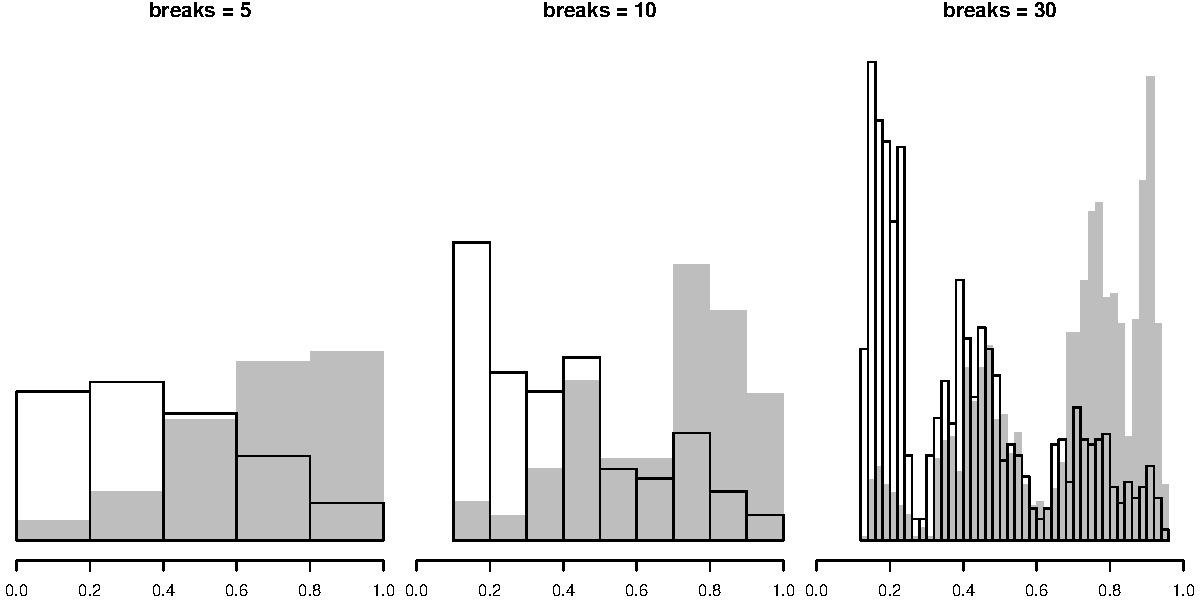
\includegraphics[width = \textwidth]{figures/pscore_stratified_hist.pdf}
\caption{基于\ri{nhanes_bmi}数据的倾向得分分布直方图：白色为对照组、灰色为处理组}\label{fig::pscore_bmi}
\end{figure}


图\ref{fig::pscore_bmi}画出了采用不同组数$(K=5,10,30)$的估计倾向得分直方图。利用第\ref{chapter::stratification-poststratification}章分析分层随机实验的\ri{Neyman_SRE}函数，可以对$K \in \{5, 10, 20, 50, 80 \}$的不同选择计算分层点估计与标准误：
\begin{lstlisting}
> pscore = glm(z ~ x, family = binomial)$fitted.values
> n.strata = c(5, 10, 20, 50, 80)
> strat.res = sapply(n.strata, FUN = function(nn){
+   q.pscore = quantile(pscore, (1:(nn-1))/nn)
+   ps.strata = cut(pscore, breaks = c(0,q.pscore,1), 
+                   labels = 1:nn)
+   Neyman_SRE(z, y, ps.strata)})
> 
> rownames(strat.res) = c("est", "se")
> colnames(strat.res) = n.strata
> round(strat.res, 3)
         5     10     20     50     80
est -0.116 -0.178 -0.200 -0.265 -0.204
se   0.283  0.282  0.279  0.272     NA
\end{lstlisting}
将$K$从$5$增至$50$降低了标准误。但不能极端地取$K=80$，因为某些层只有一个处理或对照单位，标准误无法定义。上述估计表明供餐计划对 BMI 的效应为负，但不显著。 


亦可将此法与三种传统回归法对比：不校正协变量的基础估计、Fisher法、Lin法。 
\begin{lstlisting}
> DiM = lm(y ~ z)
> Fisher = lm(y ~ z + x)
> Lin = lm(y ~ z + x + z*x)
> res.regression = c(coef(DiM)[2], hccm(DiM)[2, 2]^0.5,
+                    coef(Fisher)[2], hccm(Fisher)[2, 2]^0.5,
+                    coef(Lin)[2], hccm(Lin)[2, 2]^0.5)
> res.regression = matrix(res.regression,
+                         nrow = 2, ncol = 3)
> rownames(res.regression) = c("est", "se")
> colnames(res.regression) = c("naive", "fisher", "lin")
> round(res.regression, 3)   
    naive fisher    lin
est 0.534  0.061 -0.017
se  0.225  0.227  0.226
\end{lstlisting} 
由于协变量严重不平衡，朴素均值差与其他方法差异很大。Fisher 估计的点估计仍为正，但不显著；Lin 估计与倾向得分分层估计给出相同的定性结论。分层估计对不同$K$的选择较稳定。 




\section{倾向得分加权法}

\subsection{理论推导}

\begin{theorem}
\label{thm::pscore-weighting}
若满足$Z\ind \{ Y(1), Y(0)  \} \mid X$且$0<e(X)<1$，则
$$
E\{  Y(1) \} =  E\left\{  \frac{ZY}{e(X)}  \right\},\quad
E\{  Y(0) \} =  E\left\{  \frac{(1-Z)Y}{1-e(X)}  \right\} ,
$$
进而可得
$$
\tau = E\{  Y(1) -  Y(0) \} =  E\left\{  \frac{ZY}{e(X)} - \frac{(1-Z)Y}{1-e(X)}   \right\} .
$$
\end{theorem}


证明定理\ref{thm::pscore-weighting}前，须注意额外假设$0<e(X)<1$，称为{\it 重叠性}或{\it 正值性}条件。若某些$X$使$e(X)=0$或$1$成立，定理\ref{thm::pscore-weighting}会出现零分母。这并非倾向得分加权识别公式特有的要求：尽管定理\ref{thm::identification-formula}未明说，\eqref{eq::nonparametric-identification-tau}中识别$\tau$所需的条件期望$E(Y\mid Z=1, X)$与$ E(Y\mid Z=0, X)$，也只有在$0< e(X) < 1$时都有良好定义。重叠性可视为保证定理\ref{thm::identification-formula}和\ref{thm::pscore-weighting}公式有定义的技术条件，也涉及观察性因果推断的哲学问题。若单位$i$满足$e(X_i)=1$，总能观测其处理潜在结果$Y_i(1)$，却永远不能观测其对照潜在结果$Y_i(0)$。甚至$Y_i(0)$本身也可能没有明确含义，使单位$i$的因果效应定义变得模糊。\citet{king2006dangers}将$e(X_i)=1$时的$Y_i(0)$称为{\it 极端反事实}，并讨论了它对因果推断的危害。单位$i$满足$e(X_i)=0$时也有类似问题。 
 
 
$Z\ind \{ Y(1), Y(0)  \} \mid X$要求观测到足够协变量，以保证处理与潜在结果条件独立；$0<e(X)<1$则要求给定协变量后，处理仍保有随机性。事实上，\citet{rosenbaum1983central}对强可忽略性的原始定义同时包含这两个条件，现代文献往往将它们分开陈述。 
 


 

\begin{myproof}{定理}{\ref{thm::pscore-weighting}}这里只证明$E\{ Y(1) \}$的结论，$E\{ Y(0) \}$的证明类似。有
\begin{eqnarray*}
&&E\left\{  \frac{ZY}{e(X)}  \right\} \\
&=& E\left\{  \frac{ZY(1)}{e(X)}  \right\} \\
&=& E\left[ E\left\{  \frac{ZY(1)}{e(X)}  \mid X \right\}  \right]  \quad \text{(tower property)} \\
&=& E\left[  \frac{1}{e(X)}   E\left\{   ZY(1)  \mid X \right\}  \right]   \\
&=& E\left[  \frac{1}{e(X)}   E( Z  \mid X ) E\left\{   Y(1)  \mid X \right\}  \right]  \quad \text{(strong ignorability)} \\\\
&=& E\left[  \frac{1}{e(X)}   e(X) E\left\{   Y(1)  \mid X \right\}  \right] \\
&=& E\left[ E\left\{   Y(1)  \mid X \right\}  \right] \\
&=& E\{   Y(1) \}. 
\end{eqnarray*}
\end{myproof}



\subsection{逆倾向得分加权估计法}\label{sec::ipw-estimators}

由定理\ref{thm::pscore-weighting}，得到平均因果效应的矩估计量
$$
\hat{\tau}^\textup{ht} = \frac{1}{n} \sumn \frac{Z_i Y_i}{ \hat{e}(X_i) }
- \frac{1}{n} \sumn \frac{ (1-Z_i) Y_i}{ 1 - \hat{e}(X_i) } ,
$$
其中$\hat{e}(X_i)$为倾向得分估计。这称为逆倾向得分加权（IPW）估计量，也称 Horvitz--Thompson（HT）估计量。\citet{horvitz1952generalization}在抽样调查中提出它，\citet{rosenbaum1987model}将其用于观察性研究的因果推断。 


但$\hat{\tau}^\textup{ht}$有不少问题，特别是不具有对结果平移变换的不变性。命题\ref{prop::no-invariance-HT}精确表述了这一问题，证明留作习题\ref{hw::hajek-weights}。 

\begin{proposition}
[HT估计法的非不变性]
\label{prop::no-invariance-HT}
将$Y_i$改为$Y_i+c$，其中$c$为常数，则 HT 估计量$\hat{\tau}^\textup{ht}$变为$\hat{\tau}^\textup{ht} + c (\hat{ 1 }_\textsc{T} - \hat{ 1 }_\textsc{C})$，其中
$$
\hat{ 1 }_\textsc{T}=   \frac{1}{n} \sumn \frac{Z_i }{ \hat{e}(X_i) } ,\quad
\hat{ 1 }_\textsc{C} =\frac{1}{n} \sumn \frac{ (1-Z_i) }{ 1 - \hat{e}(X_i) }   
$$
可看作常数$1$的两个不同估计。 
\end{proposition}

命题\ref{prop::no-invariance-HT}采用了有些特别的记号$\hat{ 1 }_\textsc{T} $与$ \hat{ 1 }_\textsc{C}$：使用真实倾向得分时，这两项的期望都为 1，见习题\ref{hw::hajek-weights}。但有限样本下，$\hat{ 1 }_\textsc{T} - \hat{ 1 }_\textsc{C}$一般不为零。给所有结果加同一个常数本不应改变平均因果效应，HT 估计却依赖$c.$，因此不够理想。简单修正是分别用$\hat{ 1 }_\textsc{T}  $和$\hat{ 1 }_\textsc{C} $归一化权重，得到
$$
\hat{\tau}^\textup{hajek} = \frac{  \sumn \frac{Z_i Y_i}{ \hat{e}(X_i) }  }{  \sumn \frac{Z_i }{ \hat{e}(X_i) } }
- \frac{  \sumn \frac{ (1-Z_i) Y_i}{ 1 - \hat{e}(X_i) }  }{  \sumn \frac{ 1-Z_i}{ 1 - \hat{e}(X_i) }  }.
$$
这就是\citet{hajek1971comment}在不等概率抽样背景下提出的 Hájek 估计量。可以验证，它对平移变换不变：把$Y_i$换成$Y_i + c$后，$\hat{\tau}^\textup{hajek}$不变，见习题\ref{hw::hajek-weights}。许多数值研究还发现，在有限样本中$\hat{\tau}^\textup{hajek}$比$\hat{\tau}^\textup{ht}$稳定得多。 





\subsection{IPW方法的缺陷与因果推断的根本难题}
\label{sec::ipw-problem}


许多渐近分析要求{\it 强重叠性}条件
$$
0<  \alpha_\textsc{L} \leq e(X) \leq  \alpha_\textsc{U} < 1,
$$
即真实倾向得分与$0$和$1$保持正距离。但\citet{d2017overlap}指出，尤其在协变量较多时，这是相当强的假设，第\ref{chapter::overlap}章将详述。 


即使真实倾向得分满足强重叠性，估计倾向得分仍可能接近$0$或$1$，使加权估计量趋于极端，有限样本表现很不稳定。一种做法是截断得分，改为
$$
 \max\Big[  \alpha_\textsc{L},   \min\{   \hat{e}(X_i), \alpha_\textsc{U} \}   \Big] ,
$$
另一种做法是修剪样本，删除$\hat{e}(X_i)$位于区间$[\alpha_\textsc{L},   \alpha_\textsc{U}  ]$之外的单位。\citet{crump2009dealing}建议$  \alpha_\textsc{L} = 0.1$与$\alpha_\textsc{U} = 0.9 $，\citet{kurth2005results}建议$  \alpha_\textsc{L} = 0.05$与$\alpha_\textsc{U} = 0.95 $，\citet{yang2018asymptotic}建立了一些修剪的渐近理论。总的来说，修剪虽然常使 IPW 更稳定，也给分析增加了任意性。 




 \subsection{应用实例}\label{sec::application-pscore-weighting}


以下代码实现IPW估计及其自助法标准误计算： 
\begin{lstlisting}
ipw.est = function(z, y, x, truncps = c(0, 1))
{
  ## fitted propensity score
  pscore   = glm(z ~ x, family = binomial)$fitted.values
  pscore   = pmax(truncps[1], pmin(truncps[2], pscore))
  
  ace.ipw0 = mean(z*y/pscore - (1 - z)*y/(1 - pscore))
  ace.ipw  = mean(z*y/pscore)/mean(z/pscore) - 
    mean((1 - z)*y/(1 - pscore))/mean((1 - z)/(1 - pscore))
  
  return(c(ace.ipw0, ace.ipw))     
}


ipw.boot = function(z, y, x, n.boot = 500, truncps = c(0, 1))
{
  point.est  = ipw.est(z, y, x, truncps)
  
  ## nonparametric bootstrap
  n.sample   = length(z)
  x          = as.matrix(x)
  boot.est   = replicate(n.boot, {
    id.boot = sample(1:n.sample, n.sample, replace = TRUE)
    ipw.est(z[id.boot], y[id.boot], x[id.boot, ], truncps)
  })
  boot.se    = apply(boot.est, 1, sd)
  
  res = cbind(point.est, boot.se)
  colnames(res) = c("est", "se")
  rownames(res) = c("HT", "Hajek")
  
  return(res)
}
\end{lstlisting}

重新考虑例\ref{eg::chan-bmi-ATE}，在不同倾向得分截断下计算 IPW 估计。下面给出截断范围分别为$(0,1)$、$(0.01, 0.99)$、$(0.05, 0.95)$和$(0.1, 0.9)$时的两种加权估计及自助法标准误：
\begin{lstlisting}
> trunc.list = list(trunc0 = c(0,1), 
+                   trunc.01 = c(0.01, 0.99), 
+                   trunc.05 = c(0.05, 0.95), 
+                   trunc.1 = c(0.1, 0.9))
> trunc.est = lapply(trunc.list,
+                    function(t){
+                      est = ipw.boot(z, y, x, truncps = t)
+                      round(est, 3)
+                    })
> trunc.est
$trunc0
         est    se
HT    -1.516 0.496
Hajek -0.156 0.258

$trunc.01
         est    se
HT    -1.516 0.501
Hajek -0.156 0.254

$trunc.05
         est    se
HT    -1.499 0.501
Hajek -0.152 0.255

$trunc.1
         est    se
HT    -0.713 0.425
Hajek -0.054 0.246
\end{lstlisting}
HT 估计与此前所有其他估计差异很大，点估计的绝对值似乎过大。除采用$(0.1, 0.9)$截断外，它们都呈显著负向效应。这说明了 HT 估计的不稳定性。 



\section{倾向得分的平衡特性}


\subsection{理论推导}



\begin{theorem}
\label{thm::pscoreASbscore}
倾向得分满足
$$
Z\ind X \mid e(X) .
$$
此外，对任意函数$h(\cdot)$，只要\eqref{eq::balancehX}两侧所需矩存在，就有
\begin{eqnarray}
E\left\{   \frac{Zh(X)}{e(X)}   \right\} = E\left\{   \frac{(1-Z)h(X)}{1-e(X)}   \right\}
\label{eq::balancehX}
\end{eqnarray} 
\end{theorem}

定理\ref{thm::pscoreASbscore}不要求可忽略性，只涉及处理$Z$和协变量$X$。定理\ref{thm::pscoreASbscore}的第一部分指出，给定倾向得分后，处理指标与协变量独立，故在相同倾向得分水平内，处理组与对照组的协变量分布平衡。定理\ref{thm::pscoreASbscore}的第二部分给出了加权形式的等价平衡关系。下面证明定理\ref{thm::pscoreASbscore}。  


\begin{myproof}{定理}{\ref{thm::pscoreASbscore}}首先证明$Z\ind X \mid e(X)$，即
\begin{eqnarray}
\pr\{Z=1\mid X, e(X)\} = \pr\{Z=1\mid  e(X)\}.
\label{eq::balance1}
\end{eqnarray}
采用与定理\ref{thm::pscore-dimreduction}类似的步骤，\eqref{eq::balance1}左侧为
$$
\pr\{Z=1\mid X, e(X)\} = \pr( Z=1\mid X ) = e(X),
$$
\eqref{eq::balance1}右侧为
\begin{eqnarray*}
\pr\{Z=1\mid  e(X)\} &=& E\{  Z\mid  e(X) \}  \\
&=& E\Big[ E\{  Z\mid X,  e(X) \} \mid e(X) \Big] \\
&=& E\Big[ E\{  Z\mid X  \} \mid e(X) \Big] \\
&=& E\Big[ e(X) \mid e(X) \Big] \\
&=& e(X). 
\end{eqnarray*}
所以\eqref{eq::balance1}成立。 

其次证明\eqref{eq::balancehX}，可仿照定理\ref{thm::pscore-weighting}的证明。但利用定理\ref{thm::pscore-weighting}，还有更简单的论证：将$h(X)$视为结果时，其两个潜在结果完全相同，且可忽略性$Z\ind \{  h(X), h(X) \}  \mid X$成立。\eqref{eq::balancehX}左右之差就是$Z$对$h(X)$的平均因果效应，必为零。 
\end{myproof}





\subsection{协变量均衡性验证}
\label{sec::balance-check-bmi}

定理\ref{thm::pscoreASbscore}虽易证明，定理\ref{thm::pscoreASbscore}对实际分析却有重要启示。在查看结果数据前，就可通过数据中的协变量平衡，检查倾向得分模型是否足够合理。\citet{rubin2007design}将其视为观察性研究的设计阶段，\citet{rubin2008objective}认为，这一阶段不涉及结果值，能使因果推断更客观。\footnote{这是一项实用建议，但如何量化这种客观性并不完全清楚。} 


倾向得分分层中，得到离散估计得分$\hat{e}'(X)$，并近似有
$$
Z\ind X\mid \hat{e}'(X) = e_k\quad (k=1,\ldots, K).
$$
因此，可以检查每一得分层内，处理组与对照组的协变量分布是否相同。 


倾向得分加权中，可把$h(X)$视为伪结果，估计处理对$h(X)$的平均因果效应。由于$h(X)$上的真实平均因果效应为$0$，估计应当与$0$无显著差异。常用的$h(X)$选择是$X$。 




再次考虑例\ref{eg::chan-bmi-ATE}。采用$K=5$作倾向得分分层后，两组所有协变量都较好地平衡；Hájek 估计也有类似结果。唯一例外是图\ref{fig::balance-check}中的第七个协变量\ri{Food_Stamp}。图\ref{fig::balance-check}给出了平衡检查结果。 

\begin{figure}
\centering
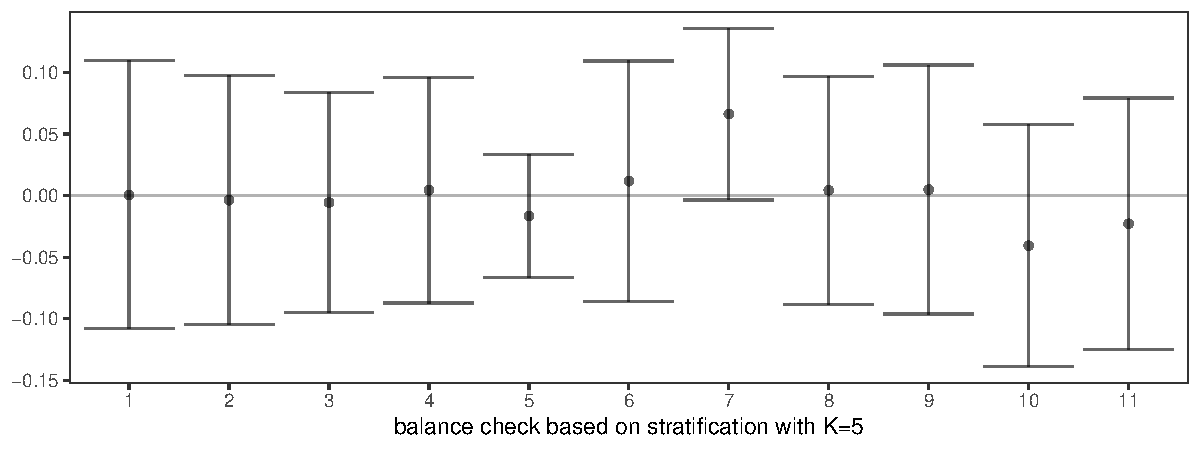
\includegraphics[width = \textwidth]{figures/balance_PSstratification5.pdf}
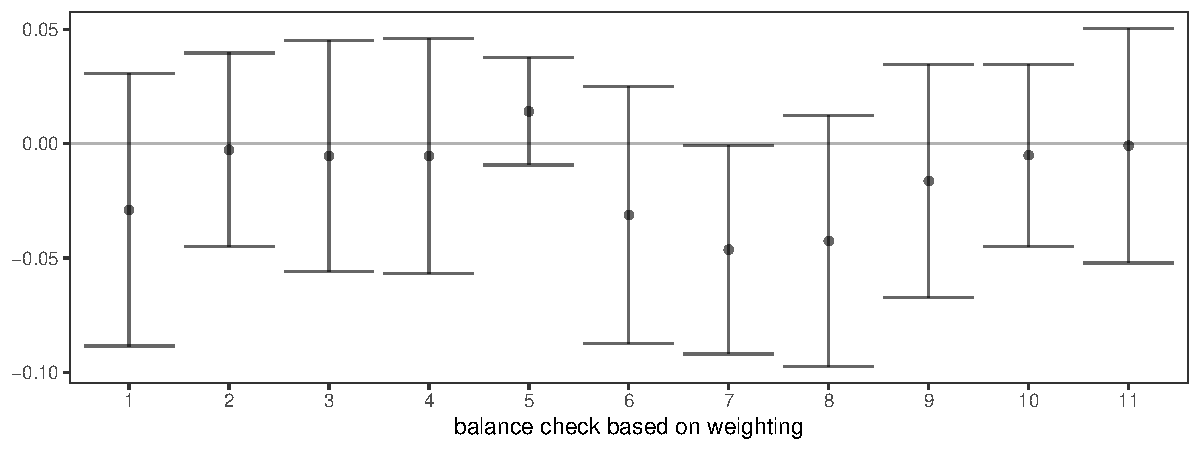
\includegraphics[width = \textwidth]{figures/balance_PShajek.pdf}
\caption{协变量均衡性检验结果：平均因果效应点估计及95\% 协变量上的平均因果效应置信区间}\label{fig::balance-check}
\end{figure}

 

 

 
 
 \section{作业习题}
 
 
 
 
 \paragraph{定理\ref{thm::pscore-dimreduction}的另一版本} \label{hw::principal-unobserved-cov}
 证明
\begin{equation}
\label{eq::principal-covariate-ind}
 Z\ind \{  Y(1), Y(0) , X\}  \mid e(X, Y(1), Y(0)   ) .
\end{equation}  
 
 注：这个结论无需强可忽略性，且蕴含
$$
  Z\ind \{  Y(1), Y(0) \}  \mid  \{ X,   e(X, Y(1), Y(0)  \} .
 $$
\citet{rosenbaum2020modern}与\citet{rosenbaum2023propensity}指出了\eqref{eq::principal-covariate-ind}的结论，将$e(X, Y(1), Y(0)   ) $称为{\it 主要未观测协变量}。 
 
 
 
\paragraph{定理\ref{thm::pscore-dimreduction}的另一版本} 

定理\ref{thm::pscore-dimreduction}在强可忽略性下成立，可忽略性下也有类似结果：若给定协变量$X$后可忽略性成立，则给定标量倾向得分$e(X)$后也成立。 

\begin{theorem}
\label{thm::pscore-dimension-reduction-weak-ig}
若对$z=0,1$有$Z\ind Y(z)  \mid X$，则对$z=0,1$有
$
Z\ind Y(z)\mid e(X)
$ 
\end{theorem} 


证明定理 \ref{thm::pscore-dimension-reduction-weak-ig}。



 
 \paragraph{IPW估计法相关问题}
\label{hw::hajek-weights} 
 
本题涉及第\ref{sec::ipw-estimators}节的 HT 估计。先证明命题\ref{prop::no-invariance-HT}，再证明
\begin{eqnarray*} 
E\left\{ \frac{1}{n} \sumn \frac{Z_i }{e(X_i) } \right\} =1,\quad
E\left\{  \frac{1}{n} \sumn \frac{ (1-Z_i) }{ 1 - e(X_i) }  \right\} = 1.
\end{eqnarray*}
最后证明，给所有观测结果$Y_i$加常数$c$后，Hájek 估计量$
\hat{\tau}^\textup{hajek} 
$保持不变。 


\paragraph{重新分析\citet{Rosenbaum::1983JRSSB}}



表\ref{table::rr1983table1}来自\citet{Rosenbaum::1983JRSSB}，研究冠状动脉搭桥手术相较药物治疗，对心导管检查后六个月功能改善的因果效应。研究者先用 74 个观测协变量估计倾向得分，再按离散得分划为 5 层。处理与结果均为二元变量，因此将数据列成表。根据表\ref{table::rr1983table1}估计平均因果效应，并报告 95\% 置信区间。 



\begin{table}
\caption{\citet{Rosenbaum::1983JRSSB}之表1}\label{table::rr1983table1}
\begin{tabular}{clcc}
\hline 
按$\hat{e}(X)$分层 & 处理方式 &  患者人数 & 改善率\\
\hline 1 & 手术 & 26 & 0.54 \\
& 药物 & 277 & 0.35 \\
2 & 手术 & 68 & 0.70 \\
& 药物 & 235 & 0.40 \\
3 & 手术 & 98 & 0.70 \\
& 药物 & 205 & 0.35 \\
4 & 手术 & 164 & 0.71 \\
& 药物 & 139 & 0.30 \\
5 & 手术 & 234 & 0.70 \\
& 药物 & 69 & 0.39 \\
\hline
\end{tabular}
\end{table}


注：感兴趣的读者可在读完第\ref{part::challenges-os}部分后，通读\citet{Rosenbaum::1983JRSSB}的论文。这是因果推断敏感性分析的经典文献。 

 


\paragraph{均衡得分与倾向得分的理论关联}
\label{hw::balancingscore-rr1983}


\citet{rosenbaum1983central}首创{\it 均衡得分}概念：

\begin{definition}
[均衡得分]\label{def::balancing-score}
  若
$$
  Z\ind X\mid b(X).
  $$
则称$b(X)$为平衡得分。
\end{definition}

定义\ref{def::balancing-score}中，$b(X)$可为标量或向量。显然，$b(X) = X$本身就是平衡得分，但没有简化原协变量，实用价值有限。由定理\ref{thm::pscoreASbscore}，倾向得分是平衡得分的特例。更有意思的是，\citet{rosenbaum1983central}证明倾向得分是最粗的平衡得分，见下面的定理\ref{thm::balancingscore}，其中包含定理\ref{thm::pscoreASbscore}这一特例。 


\begin{theorem}
\label{thm::balancingscore}
$b(X)$是平衡得分，当且仅当$b(X)$至少与$e(X)$同样精细，即存在函数$f(\cdot)$使$e(X) = f(b(X))$。 
\end{theorem}


定理\ref{thm::balancingscore}与亚组分析有关。除平均因果效应$\tau$，也可能关心亚组效应，例如分别估计男孩与女孩的平均因果效应。不失一般性，令$X$的第一分量表示是否为女孩，目标为
$$
\tau(x_1) = E\{ Y(1) - Y(0) \mid X_1 = x_1  \},\quad (x_1=1,0).
$$
由定理\ref{thm::balancingscore}，在可忽略性下还有
\begin{equation}
\label{eq::subgroup-ignorability}
Z\ind \{ Y(1) , Y(0) \} \mid e(X), X_1
\end{equation}
因为$b(X) = \{e(X), X_1\}$比$e(X)$更精细，所以也是平衡得分。\eqref{eq::subgroup-ignorability}的条件独立性保证，在$X_1$的每个水平内，给定倾向得分后可忽略性仍成立。因此，可在$X_1$的各水平内分别作同样的倾向得分分析，得到两个亚组效应的估计。 


根据上述动机，证明定理\ref{thm::balancingscore}。 


\paragraph{亚组效应估计的基础问题}

本题与习题\ref{hw::balancingscore-rr1983}有关，但可独立完成。 

考虑协变量为$X = (X_1, X_2)$的标准观察性研究，其中$X_1$是二元亚组指标，例如是否为统计学专业，$X_2$为其余协变量。目标参数是亚组因果效应
$$
\tau(x_1) = E\{ Y(1) - Y(0) \mid X_1 = x_1  \},\quad (x_1=1,0).
$$
证明
$$
\tau(x_1) =  E\left\{   \frac{  1(X_1 = x_1) ZY}{ e(X) }   - \frac{  1(X_1 = x_1) (1-Z)Y}{ 1 -  e(X) }    \right\} \Big /  \pr(X_1 = x_1)
$$
并给出$\tau(x_1) $对应的 HT 和 Hájek 估计量。 



 \paragraph{推荐阅读}
 
 
本章标题与\citet{rosenbaum1983central}的经典论文相同，多数结论直接取自该文。  


\citet{rubin2007design}与\citet{rubin2008objective}强调，观察性研究的设计阶段对更客观的因果推断很重要。 
 
  
 
\chapter{用于估计平均因果效应的双重稳健估计量或增强型逆倾向得分加权估计量}\label{chapter::doubly-robust}
 \chaptermark{双重稳健估计量}

在可忽略性条件 $Z\ind \{ Y(1), Y(0) \} \mid X$ 以及重叠条件 $0< e(X) < 1$ 下，第 \ref{chapter::pscore-key} 章已给出了平均因果效应 $\tau = E\{ Y(1) - Y(0)  \}$ 的两种识别公式。第一种是结果回归公式：
\begin{eqnarray}
\tau  =  E\{ \mu_1(X) \} - E\{ \mu_0(X) \} \label{eq::iden-outreg}
\end{eqnarray}
其中
\begin{eqnarray*}
\mu_1(X)  &=& E\{  Y(1) \mid X \} = E(Y\mid Z=1, X),\\ 
\mu_0(X) &=& E\{  Y(0) \mid X \} = E(Y\mid Z=0, X)
\end{eqnarray*}
分别为处理组和对照组下结果变量的条件均值函数。第二种是逆倾向得分加权（IPW）公式：
\begin{eqnarray}
\tau = E\left\{  \frac{ZY}{e(X)}   \right\} - E\left\{  \frac{(1-Z)Y}{1-e(X)}   \right\} \label{eq::iden-ipw}
\end{eqnarray}
此处
$$
e(X) = \pr(Z=1\mid X)
$$
即为第 \ref{chapter::pscore-key} 章中定义的倾向得分。  


结果回归估计量需要针对处理组和对照组分别拟合结果模型；若模型设定正确则该估计量具有一致性。IPW估计量则需拟合基于协变量的倾向得分模型；若倾向得分模型设定正确则该估计量也具有一致性。 


从数学上看，由 \eqref{eq::iden-outreg} 和 \eqref{eq::iden-ipw} 可推导出无数种平均因果效应的识别公式。下文我将介绍一种具有良好理论性质的特殊组合形式。该组合形式能确保：只要倾向得分模型或结果模型其中之一设定正确，相应估计量便具有一致性。这种估计量即由 James Robins 所倡导的{\it 双重稳健}估计量 \citep{scharfstein1999adjusting, bang2005doubly}。 



\section{双重稳健估计量}

\subsection{总体层面的定义}


为结果条件均值设定模型$\mu_1(X, \beta_1)$与$\mu_0(X, \beta_0)$，参数分别为$\beta_1$与$\beta_0$。例如，工作模型为线性或逻辑模型时，参数就是回归系数。结果模型设定正确时，$\mu_1(X, \beta_1) = \mu_1(X)$且$   \mu_0(X, \beta_0) = \mu_0(X)$。再为倾向得分设定工作模型$e(X, \alpha)$，参数为$\alpha$；例如使用逻辑模型时，$\alpha$为回归系数。倾向得分模型正确时，$e(X,\alpha) = e(X)$。实践中两种模型都可能误设，因此称为{\it 工作模型}。 

定义如下量：
\begin{eqnarray}
\tilde{\mu}_1^\textup{dr} &=& E\left[   \frac{Z\{ Y-\mu_1(X,\beta_1) \}}{  e(X,\alpha) }   + \mu_1(X, \beta_1)  \right] , \label{eq::dr-aug-out1}   \\
\tilde{\mu}_0^\textup{dr} &=& E\left[   \frac{(1-Z)\{ Y-\mu_0(X,\beta_0) \}}{  1-e(X,\alpha) }   + \mu_0(X, \beta_0)  \right]  , \label{eq::dr-aug-out0} 
\end{eqnarray}
该式亦可改写为
\begin{eqnarray}
\tilde{\mu}_1^\textup{dr} &=& E\left[   \frac{Z Y}{  e(X,\alpha) }   - \frac{  Z -  e(X,\alpha)  }{ e(X,\alpha) } \mu_1(X, \beta_1)  \right]  ,\label{eq::dr-aug-ipw1} \\
\tilde{\mu}_0^\textup{dr} &=& E\left[   \frac{(1-Z) Y}{  1-e(X,\alpha) }    - \frac{ e(X,\alpha)-Z  }{1- e(X,\alpha)} \mu_0(X, \beta_0)  \right]    .\label{eq::dr-aug-ipw0} 
\end{eqnarray}
 
\eqref{eq::dr-aug-out1} 和 \eqref{eq::dr-aug-out0} 本质上是在结果回归估计量基础上引入了倾向得分加权修正项；而 \eqref{eq::dr-aug-ipw1} 与 \eqref{eq::dr-aug-ipw0} 则体现了用预测结果值修正 IPW 估计量的思想。正因如此，双重稳健估计量亦被称为{\it 增强型逆倾向得分加权}（AIPW）估计量。 



这种修正方式能显著优化估计量的理论性质。   
 
 


\begin{theorem}
\label{thm::doublyrobust}
假设满足可忽略性条件 $Z \ind  \{  Y(1), Y(0) \} \mid X$ 以及重叠条件 $0 < e(X) < 1$。则： 
\begin{enumerate}
\item
若 $e(X,\alpha) = e(X)$ 或 $\mu_1(X, \beta_1) = \mu_1(X)$ 任一条件成立，则 $\tilde{\mu}_1^\textup{dr} = E\{  Y(1) \}$。
\item 
若 $e(X,\alpha) = e(X)$ 或 $\mu_0(X, \beta_0) = \mu_0(X)$ 任一条件成立，则 $\tilde{\mu}_0^\textup{dr} = E\{  Y(0) \}$。
\item 
若 $e(X,\alpha) = e(X)$ 或者 $\{\mu_1(X, \beta_1) = \mu_1(X),   \mu_0(X, \beta_0) = \mu_0(X)\}$ 任一条件成立，则 $\tilde{\mu}_1^\textup{dr} - \tilde{\mu}_0^\textup{dr} = \tau$。 
\end{enumerate}
\end{theorem}


由定理 \ref{thm::doublyrobust} 可知：只要倾向得分模型或结果模型其中之一设定正确，$\tilde{\mu}_1^\textup{dr} - \tilde{\mu}_0^\textup{dr} $ 的值便等于真实因果效应 $\tau$，这也正是该估计量被称为“双重稳健”的原因。  


\begin{myproof}{定理}{\ref{thm::doublyrobust}}这里只证明$\mu_1 = E\{  Y(1) \}$的结论，$\mu_0 = E\{  Y(0) \}$的证明类似。 


有如下分解
\begin{eqnarray*}
&&\tilde{\mu}_1^\textup{dr} - E\{  Y(1) \}     \\
&=& E\left[   \frac{Z\{ Y(1)-\mu_1(X,\beta_1) \}}{  e(X,\alpha) }   - \{ Y(1) -  \mu_1(X, \beta_1) \} \right]  
\qquad (\text{by definition})\\
&=&    E\left[   \frac{Z - e(X,\alpha) }{  e(X,\alpha) }   \{ Y(1) -  \mu_1(X, \beta_1) \} \right]  
\qquad (\text{combining terms})\\
&=&  E\left(  E\left[   \frac{Z - e(X,\alpha) }{  e(X,\alpha) }   \{ Y(1) -  \mu_1(X, \beta_1) \} \mid X \right] \right) 
\qquad (\text{tower property})\\
&=& E\left[  E\left\{   \frac{Z - e(X,\alpha) }{  e(X,\alpha) } \mid X \right\} \times E\left\{  Y(1) -  \mu_1(X, \beta_1)  \mid X \right\} \right] 
\qquad (\text{ignorability})\\
&=& E\left[   \frac{e(X) - e(X,\alpha) }{  e(X,\alpha) }  \times  \left\{  \mu_1(X) -  \mu_1(X, \beta_1)   \right\} \right]  . 
\end{eqnarray*}
所以，只要$e(X,\alpha) = e(X)$或$\mu_1(X, \beta_1) = \mu_1(X)$成立，就有$\tilde{\mu}_1^\textup{dr} - E\{  Y(1) \}  = 0$。 
\end{myproof}



 

\subsection{样本层面的实现}


基于总体层面的 $\tilde{\mu}_1^\textup{dr} $ 与 $\tilde{\mu}_0^\textup{dr} $，我们可以构造对应的样本估计量以计算 $\tau$ 的值。


\begin{definition}
[平均因果效应的双重稳健估计量]\label{def::dr:ace}
根据数据$(X_i, Z_i, Y_i)_{i=1}^n$，可按以下步骤构造$\tau$的双重稳健估计量。\footnote{此前不强调工作模型参数时，用$\hat e(X_i)$表示$e(X_i, \hat{\alpha})$，用$ \hat \mu_z(X_i) $表示$ \mu_z(X_i, \hat{\beta}_1) $。} 
\begin{enumerate}
[(1)]
\item
计算倾向得分的拟合值：$e(X_i, \hat{\alpha})$； 
\item
计算结果均值的拟合值：$ \mu_1(X_i, \hat{\beta}_1) $ 与 $ \mu_0(X_i, \hat{\beta}_0) $； 
\item
构造双重稳健估计量$\hat{\tau}^\textup{dr} = \hat{\mu}_1^\textup{dr}  - \hat{\mu}_0^\textup{dr}$，其中
$$
 \hat{\mu}_1^\textup{dr}  = \frac{1}{n} \sumn \left[ \frac{Z_i\{ Y_i-\mu_1(X_i,\hat{\beta}_1) \}}{  e(X_i, \hat{\alpha}) }   + \mu_1(X_i, \hat{\beta}_1) \right]
$$
和
$$
 \hat{\mu}_0^\textup{dr}  = \frac{1}{n} \sumn \left[  \frac{(1-Z_i)\{ Y_i-\mu_0(X_i, \hat{\beta}_0) \}}{  1-e(X_i,\hat{\alpha}) }   + \mu_0(X_i, \hat{\beta}_0)       \right] . 
$$
\end{enumerate}
\end{definition}

根据定义\ref{def::dr:ace}，双重稳健估计量也可写为
$$
\hat{\tau}^\textup{dr} =\hat{\tau}^\textup{reg}  + 
\frac{1}{n} \sumn  \frac{Z_i\{ Y_i-\mu_1(X_i,\hat{\beta}_1) \}}{  e(X_i, \hat{\alpha}) } 
-  \frac{1}{n} \sumn   \frac{(1-Z_i)\{ Y_i-\mu_0(X_i, \hat{\beta}_0) \}}{  1-e(X_i,\hat{\alpha}) }  . 
$$
仿照\eqref{eq::dr-aug-ipw1}与\eqref{eq::dr-aug-ipw0}，还可改写为
$$
\hat{\tau}^\textup{dr} = \hat{\tau}^\textup{ipw}  
  - \frac{1}{n} \sumn    \frac{  Z_i -  e(X_i, \hat\alpha)  }{ e(X_i, \hat\alpha) } \mu_1(X_i, \hat\beta_1)
  + \frac{1}{n} \sumn    \frac{ e(X_i, \hat\alpha)-Z_i  }{1- e(X_i,\hat \alpha)} \mu_0(X_i, \hat\beta_0) .
$$ 

 
\citet{funk2011doubly}建议从$(Z_i, X_i, Y_i)_{i=1}^n$重抽样，用非参数自助法近似$\hat{\tau}^\textup{dr}$的方差。
 

\section{双重稳健估计量的更多直观解释与理论}

本章开头指出，结果回归与 IPW 的基本识别公式能立即产生无穷多个其他识别公式，但\eqref{eq::dr-aug-out1}和\eqref{eq::dr-aug-out0}这种特定双重稳健形式并不容易直接想到。\eqref{eq::dr-aug-out1}与\eqref{eq::dr-aug-out0}最初由理论推导而来，依赖高等数理统计中的{\it 半参数效率理论}\citep{bickel1993efficient}，超出本书范围。下面给出构造\eqref{eq::dr-aug-out1}和\eqref{eq::dr-aug-out0}的两个直观视角。第\ref{sec::improving-ipw}与\ref{sec::improving-outreg}节都只讨论$E\{ Y(1) \}$，$E\{ Y(0) \}$的估计由对称性类似可得。 



\subsection{降低 IPW 估计量的方差}\label{sec::improving-ipw}


基于
$$
\mu_1 = E\left\{   \frac{ZY}{e(X)}   \right\}
$$
的$\mu_1$ IPW 估计，完全忽略$Y$的结果模型。其优点是不假定结果模型仍可一致。但若协变量能预测结果，即使工作结果模型有误，残差的方差通常也小于结果本身。对可能误设的模型$\mu_1(X, \beta_1)$，总有分解
$$
\mu_1  = E\{ Y(1) \} = E\{ Y(1)  -\mu_1(X, \beta_1) \} + E\{\mu_1(X, \beta_1)\}.
$$
将$Y(1)  -\mu_1(X, \beta_1)$视为处理下的“伪潜在结果”，对第一项应用 IPW，得
\begin{eqnarray}
\mu_1  &=& E\left\{ \frac{Z \{Y  -\mu_1(X, \beta_1) \}}{e(X)} \right\} + E\{\mu_1(X, \beta_1)\}  \label{eq::explain-ipw-efficiency-basic}  \\
&=& E\left\{ \frac{Z \{Y  -\mu_1(X, \beta_1) \}}{e(X)}  +  \mu_1(X, \beta_1) \right\} ,\label{eq::explain-ipw-efficiency}
\end{eqnarray}
只要倾向得分模型正确，公式成立，无须结果模型正确。利用工作模型提高效率是抽样调查中的旧思想，\citet{little2004robust}和\citet{lumley2011connections}指出了它与双重稳健估计的联系。   



\subsection{降低结果回归估计量的偏差}\label{sec::improving-outreg}


第\ref{sec::improving-ipw}节从 IPW 出发，利用工作结果模型提高效率。也可从结果回归估计
$$
\tilde{\mu}_1 = E\{\mu_1(X, \beta_1)\} 
$$
出发。若模型错误，它未必等于$\mu_1$，偏差为$ E\{\mu_1(X, \beta_1)  -  Y(1)\}   $。只要倾向得分模型正确，可用 IPW 估计该偏差：
$$
B = 
E\left\{ \frac{Z \{\mu_1(X, \beta_1) - Y\}}{e(X)} \right\} 
$$
因此，去偏后的估计为$
\tilde{\mu}_1 - B  ,
$，恰好等于\eqref{eq::explain-ipw-efficiency}。 


\section{示例}
\label{sec::dr-examples}


\subsection{$\tau$的若干常用估计量汇总}


下面的\ri{R}代码实现$\tau$的结果回归、HT、Hájek 和双重稳健估计，可方便地根据\ri{glm}函数的拟合值计算。倾向得分默认采用逻辑模型，结果默认采用线性模型，指定\ri{out.family = gaussian}。\footnote{\ri{glm}比\ri{lm}更一般；指定\ri{out.family = gaussian}时，\ri{glm}与\ri{lm}相同。}二元结果也可指定\ri{out.family = binomial}拟合逻辑模型。

\begin{lstlisting}
OS_est = function(z, y, x, out.family = gaussian, 
                  truncps = c(0, 1))
{
     ## fitted propensity score
     pscore   = glm(z ~ x, family = binomial)$fitted.values
     pscore   = pmax(truncps[1], pmin(truncps[2], pscore))
     
     ## fitted potential outcomes
     outcome1 = glm(y ~ x, weights = z, 
                    family = out.family)$fitted.values
     outcome0 = glm(y ~ x, weights = (1 - z), 
                    family = out.family)$fitted.values
     
     ## outcome regression estimator
     ace.reg  = mean(outcome1 - outcome0) 
     ## IPW estimators
     y.treat     = mean(z*y/pscore)
     y.control   = mean((1 - z)*y/(1 - pscore))
     one.treat   = mean(z/pscore)
     one.control = mean((1 - z)/(1 - pscore))
     ace.ipw0    = y.treat - y.control
     ace.ipw     = y.treat/one.treat - y.control/one.control
     ## doubly robust estimator
     res1      = y - outcome1
     res0      = y - outcome0
     r.treat   = mean(z*res1/pscore)
     r.control = mean((1 - z)*res0/(1 - pscore))
     ace.dr    = ace.reg + r.treat - r.control

     return(c(ace.reg, ace.ipw0, ace.ipw, ace.dr))     
}
\end{lstlisting}


这些估计量的解析方差公式推导繁琐，可从$\{ Z_i, X_i, Y_i \}_{i=1}^n$重抽样，用自助法方便地近似方差。下面的函数基于前面的\ri{OS_est}，返回点估计及自助法标准误。 


\begin{lstlisting}
OS_ATE = function(z, y, x, n.boot = 2*10^2,
                     out.family = gaussian, truncps = c(0, 1))
{
     point.est  = OS_est(z, y, x, out.family, truncps)
     
     ## nonparametric bootstrap
     n          = length(z)
     x          = as.matrix(x)
     boot.est   = replicate(n.boot, {
       id.boot = sample(1:n, n, replace = TRUE)
       OS_est(z[id.boot], y[id.boot], x[id.boot, ], 
              out.family, truncps)
     })

     boot.se    = apply(boot.est, 1, sd)
     
     res        = rbind(point.est, boot.se)
     rownames(res) = c("est", "se")
     colnames(res) = c("reg", "HT", "Hajek", "DR")
     
     return(res)
}
\end{lstlisting}




\subsection{模拟}
\label{sec::dr-simulation}


下面用模拟评价四种情形下估计量的有限样本性质：
\begin{enumerate}
\item\label{case::11}
倾向得分模型与结果模型均正确；
\item\label{case::01}
倾向得分模型错误，结果模型正确；
\item\label{case::10}
倾向得分模型正确，结果模型错误；
\item\label{case::00}
倾向得分模型与结果模型均错误。
\end{enumerate}
报告模拟中估计量的平均偏差、真实标准误及估计标准误的平均值。 



情形\ref{case::11}的数据生成过程为
\begin{lstlisting}
  x       = matrix(rnorm(n*2), n, 2)
  x1      = cbind(1, x)
  beta.z  = c(0, 1, 1)
  pscore  = 1/(1 + exp(- as.vector(x1%*%beta.z)))
  z       = rbinom(n, 1, pscore)
  beta.y1 = c(1, 2, 1)
  beta.y0 = c(1, 2, 1)
  y1      = rnorm(n, x1%*%beta.y1)
  y0      = rnorm(n, x1%*%beta.y0)
  y       = z*y1 + (1 - z)*y0
\end{lstlisting}
情形\ref{case::01}将倾向得分模型改为非线性：
\begin{lstlisting}
  x1      = cbind(1, x, exp(x))
  beta.z  = c(-1, 0, 0, 1, -1)
  pscore  = 1/(1 + exp(- as.vector(x1%*%beta.z)))
\end{lstlisting}
情形\ref{case::10}将结果模型改为非线性： 
\begin{lstlisting}
  beta.y1 = c(1, 0, 0, 0.2, -0.1)
  beta.y0 = c(1, 0, 0, -0.2, 0.1)
  y1      = rnorm(n, x1%*%beta.y1)
  y0      = rnorm(n, x1%*%beta.y0)
\end{lstlisting}
情形\ref{case::00}同时修改倾向得分与结果模型。 


样本量设为$n=500$，按上述数据生成过程生成$500$个独立数据集。在情形\ref{case::11}中， 
\begin{lstlisting}
          reg   HT Hajek   DR
ave.bias 0.00 0.02  0.03 0.01
true.se  0.11 0.28  0.26 0.13
est.se   0.10 0.25  0.23 0.12
\end{lstlisting}
全部估计量都近似无偏，两种加权估计量的方差较大。在情形\ref{case::01}中，
\begin{lstlisting}
          reg    HT Hajek    DR
ave.bias 0.00 -0.76 -0.75 -0.01
true.se  0.12  0.59  0.47  0.18
est.se   0.13  0.50  0.38  0.18
\end{lstlisting}
由于倾向得分误设，两种加权估计严重有偏；结果回归与双重稳健估计近似无偏。 


在情形\ref{case::10}中，
\begin{lstlisting}
           reg   HT Hajek   DR
ave.bias -0.05 0.00 -0.01 0.00
true.se   0.11 0.15  0.14 0.14
est.se    0.11 0.14  0.13 0.14
\end{lstlisting}
由于结果模型误设，结果回归估计的偏差大于其他三种；加权估计与双重稳健估计近似无偏。 


在情形\ref{case::00}中，
\begin{lstlisting}
           reg   HT Hajek   DR
ave.bias -0.08 0.11 -0.07 0.16
true.se   0.13 0.32  0.20 0.41
est.se    0.13 0.25  0.16 0.26
\end{lstlisting}
由于两个模型都错误，全部估计量有偏。HT 与双重稳健估计的偏差最大。两个模型都错误时，双重稳健估计反而显得“双重脆弱”。 


以上所有情形中，只要估计量对真实平均因果效应近似无偏，自助法标准误就接近真实标准误。 




\subsection{应用}
\label{sec::ATE-application}




重新考虑例\ref{eg::chan-bmi-ATE}，得到如下估计及自助法标准误：
\begin{lstlisting}
       reg     HT  Hajek     DR
est -0.017 -1.516 -0.156 -0.019
se   0.230  0.492  0.246  0.233
\end{lstlisting}
两种加权估计的绝对值远大于其他两种。将倾向得分截断在$[0.1, 0.9]$内，得到以下估计及自助法标准误：
\begin{lstlisting}
       reg     HT  Hajek     DR
est -0.017 -0.713 -0.054 -0.043
se   0.223  0.422  0.235  0.231
\end{lstlisting}
Hájek 估计变得更接近结果回归与双重稳健估计，Horvitz--Thompson 估计仍明显偏离。 



\section{进一步讨论}



回顾定理\ref{thm::doublyrobust}的证明，双重稳健性的关键是乘积结构
$$
\tilde{\mu}_1^\textup{dr} - E\{  Y(1) \} 
= E\left[   \frac{e(X) - e(X,\alpha) }{  e(X,\alpha) }  \times  \left\{  \mu_1(X) -  \mu_1(X, \beta_1)   \right\} \right] ,
$$
它保证，只要$e(X) = e(X,\alpha) $或$ \mu_1(X) =  \mu_1(X, \beta_1) $，估计误差就为零。但两个模型都错误时，这一结构也可能带来“双重脆弱性”：两个误差相乘，可能产生更大的误差。第\ref{sec::dr-simulation}节的模拟验证了这一点。 


\citet{kang2007demystifying}通过模拟批评双重稳健估计，发现其有限样本表现甚至可能比简单结果回归与 IPW 更不稳定。尽管受到\citet{kang2007demystifying}批评，自\citet{scharfstein1999adjusting}的开创性工作以来，它已成为因果推断的标准策略。近来，统计与计量经济学理论以更时髦的“双重机器学习”名称重新研究它\citep{chernozhukov2018double}：基本思想是用机器学习替代倾向得分和结果的工作模型，比传统参数模型更灵活。 





\section{作业习题}



 \paragraph{实例分析}\label{hw::discreteX-obs}
考虑离散协变量$X \in \{1, \ldots, K\}$，目标参数为$\tau$。不施加模型限制时，第$X=k\ (k=1, \ldots, K)$层的倾向得分估计$\hat{e}(X)$为处理比例$\hat{e}_{[k]} = \hat{\pr}(Z=1\mid X=k) $，结果均值估计为处理组与对照组各自的样本均值$\hat{\bar{Y}}_{[k]}(1)  = \hat{E}(Y\mid Z=1, X=k) $与$\hat{\bar{Y}}_{[k]}(0)  = \hat{E}(Y\mid Z=0, X=k) $。证明分层、结果回归、HT、Hájek 和双重稳健估计量在数值上完全相同。 
 


\paragraph{$\tau$双重稳健估计量的另一形式}\label{hw::alternative-dr2-robins}

由\eqref{eq::explain-ipw-efficiency-basic}启发，可得$\mu_1 = E\{ Y(1) \} $的另一种双重稳健形式：
$$
\tilde{\mu}_1^\text{dr2} = 
\frac{ E\left[   \frac{Z\{ Y-\mu_1(X,\beta_1) \}}{  e(X,\alpha) } \right] }{E\left[   \frac{Z }{  e(X,\alpha) } \right]} 
 + E\{ \mu_1(X, \beta_1)  \} .
$$
证明，只要$e(X,\alpha)  = e(X)$或$\mu_1(X, \beta_1) =  \mu_1(X)$，便有$\tilde{\mu}_1^\text{dr2} = \mu_1$。给出估计$\mu_0$的类似公式，并据此给出$\tau$双重稳健估计量的样本对应式。 

注：这一双重稳健形式见于\citet{robins2007comment}。 



\paragraph{双重稳健估计偏差的上界}\label{hw::upperbound-dr}


考虑用于估计$E\{  Y(1) \} $的总体双重稳健形式$\tilde{\mu}_1^\textup{dr} $，证明
$$
 |   \tilde{\mu}_1^\textup{dr} - E\{  Y(1) \}  |  \leq
\sqrt{
E\left[   \frac{ \{  e(X) - e(X,\alpha)\}^2  }{  e(X,\alpha)^2 }  \right] \times 
E\left[  \left\{  \mu_1(X) -  \mu_1(X, \beta_1)   \right\}^2 \right] .
}
$$
再求$\tilde{\mu}_0^\textup{dr} $估计$E\{  Y(0) \} $时偏差的类似上界。 


注：证明可参考第\ref{sec::cauchy-schwarz-inequality}节。 


\paragraph{例\ref{eg::job-training-obs}的数据分析}


运用前文所述方法分析数据集 \ri{cps1re74.csv}。 

 
 
\paragraph{分析 Karolinska 研究所的数据集}\label{hw::Karolinska-dr}
 
 \citet{rubin2008objective}用\texttt{karolinska.txt}说明观察性因果推断。数据包含 1988—1995 年在瑞典中部与北部确诊的 158 名贲门癌患者，其中 79 人在高诊疗量医院确诊，即该时期诊治此类患者超过十人的医院；另 79 人在其他低诊疗量医院确诊。处理\texttt{z}表示是否在高诊疗量医院确诊，结果\texttt{y}表示确诊后是否存活超过一年。协变量\texttt{x}包含年龄、是否来自农村及是否为男性等信息。 
 
\begin{lstlisting}
karolinska = read.table("karolinska.txt", header = TRUE)
z = karolinska$hvdiag
y = 1 - (karolinska$year.survival == 1)
x = as.matrix(karolinska[, c(3, 4, 5)])
\end{lstlisting}


用迄今介绍的方法分析该数据集。 



 \paragraph{推荐阅读}
 
 \citet{lunceford2004stratification} 系统综述了第 \ref{chapter::pscore-key} 与 \ref{chapter::doubly-robust} 章所述各类估计量的特性。 
 

  
  
\chapter{处理组单元的平均因果效应及其他估计量}
 \label{chapter::ATT-and-other}

第\ref{chapter::observational-studies}章至第\ref{chapter::doubly-robust}章主要讨论了在可忽略性假设与重叠性假设下，平均因果效应$\tau = E\{  Y(1) - Y(0) \}$的识别与估计。从概念上讲，将讨论范围扩展至处理组与对照组单元的平均因果效应是顺理成章的：
\begin{eqnarray*}
\tau_\textsc{T}  &=&  E\{  Y(1) - Y(0) \mid Z=1 \} ,  \\
\tau_\textsc{C}  &=&  E\{  Y(1) - Y(0) \mid Z=0 \} . 
\end{eqnarray*}
若$\tau_\textsc{T}$与$\tau_\textsc{C}$均不等于$\tau$，则说明处理组与对照组间的平均因果效应存在异质性。究竟应当估计$\tau_\textsc{T}$、$\tau_\textsc{C}$还是$\tau$，则需视具体研究问题而定。 


由于二者具有对称性，本章重点探讨$\tau_\textsc{T} $。第\ref{sec::other-estmand-overlap}章还会探讨其他估计量的相关问题。 



\section{$\tau_\textsc{T} $的非参数识别}


处理组单元的平均因果效应可表示为
$$
\tau_\textsc{T} = E(Y\mid Z=1) -  E\{    Y(0) \mid Z=1 \},
$$
其中第一项$E(Y\mid Z=1) $可直接由数据识别；第二项$E\{    Y(0) \mid Z=1 \}$则为反事实值。识别该项的经典假设即为前述的可忽略性与重叠性假设。



\begin{assumption}
\label{assume::ignorability-y0}
$Z\ind Y(0) \mid X$且$e(X) < 1$。 
\end{assumption}

由于识别的关键在于确定$E\{    Y(0) \mid Z=1 \}$，因此仅需“单边”的可忽略性与重叠性假设即可。在假设\ref{assume::ignorability-y0}下，可得到关于$\tau_\textsc{T} $的如下识别结果： 


\begin{theorem}
\label{thm::identification-ATT}
在假设\ref{assume::ignorability-y0}成立时，有
\begin{eqnarray*}
 E\{    Y(0) \mid Z=1 \}  &=& E\left\{  E(    Y \mid Z=0 , X) \mid  Z=1  \right\} \\
 &=&  \int  E(    Y \mid Z=0 , X=x) f(  x \mid Z=1) \diff x .
\end{eqnarray*}
\end{theorem}


依据定理\ref{thm::identification-ATT}，反事实均值$ E\{    Y(0) \mid Z=1 \}  $等同于在给定处理组协变量分布的条件下，对照组观测结果的条件均值。这意味着$\tau_\textsc{T} $可通过下式实现非参数识别：
\begin{equation}
\tau_\textsc{T}  = E(Y\mid Z=1) -E\left\{  E(    Y \mid Z=0 , X) \mid  Z=1  \right\}  \label{eq::att-identification} 
\end{equation}

\begin{myproof}{定理}{\ref{thm::identification-ATT}}有
\begin{eqnarray*}
 E\{    Y(0) \mid Z=1 \} &=&  E\big[   E\{    Y(0) \mid Z=1 , X\} \mid  Z=1  \big] \\
 &=& E\big[   E\{    Y(0) \mid Z=0 , X\} \mid  Z=1  \big] \\
 &=& E\left\{  E(    Y \mid Z=0 , X) \mid  Z=1  \right\} \\
 &=& \int  E(    Y \mid Z=0 , X=x) f(  x \mid Z=1)  \diff x.
\end{eqnarray*}
\end{myproof}


若$X$离散，定理\ref{thm::identification-ATT}的识别公式简化为
$$
 E\{    Y(0) \mid Z=1 \}  = \sum_{k=1}^K E(    Y \mid Z=0 , X=k) \pr(X=k \mid  Z=1  ),
$$
%
%Under Assumption \ref{assume::ignorability-y0}, we have 
%\begin{eqnarray*}
% E\{    Y(0) \mid Z=1 \} &=&  E\big[   E\{    Y(0) \mid Z=1 , X\} \mid  Z=1  \big] \\
% &=& E\big[   E\{    Y(0) \mid Z=0 , X\} \mid  Z=1  \big] \\
% &=& E\left\{  E(    Y \mid Z=0 , X) \mid  Z=1  \right\} ,
%\end{eqnarray*}
%therefore, we can identify $\tau_\textsc{T}$ by
%\begin{eqnarray} 
%\tau_\textsc{T}  &=& E(Y\mid Z=1) -E\left\{  E(    Y \mid Z=0 , X) \mid  Z=1  \right\}  \label{eq::att-identification}  \\
%&=& E(Y\mid Z=1) - \sum_{k=1}^K E(    Y \mid Z=0 , X=k) \pr(X=k \mid  Z=1  )  \nonumber \\
%&=& E(Y\mid Z=1) - \int  E(    Y \mid Z=0 , X=x) F( \text{d} x \mid Z=1),  \nonumber 
%\end{eqnarray} 
%where $F( x \mid Z=1)$ is the distribution function of the covariates among treated units. 
%For discrete $X$, we can use
由此得到$\tau_\textsc{T} $的分层估计量：
$$
\hat{\tau}_\textsc{T} =   \hat{\bar{Y}}(1) - \sum_{k=1}^K \hat{\pi}_{[k]\mid 1} \hat{\bar{Y}}_{[k]}(0),
$$
其中$\hat{\pi}_{[k]\mid 1} = n_{[k]1}/n_1$是处理单位中协变量$X$属于第$k$类的比例。 


对于连续型$X$，则需借助对照组数据拟合$E(Y\mid Z=0, X)$的模型。若拟合所得处理组潜在结果为$\hat{\mu}_0(X_i)$，则相应估计量为
$$
\hat{\tau}_\textsc{T}^\text{reg} =  \hat{\bar{Y}}(1) - n_1^{-1} \sumn Z_i \hat{\mu}_0(X_i) = n_1^{-1} \sumn Z_i  \{  Y_i - \hat{\mu}_0(X_i)  \}. 
$$


\begin{example}\label{eg::att-regression1}
若为所有单元设定如下线性模型
$$
E(Y\mid Z, X) = \beta_0  + \beta_z  Z + \beta_x\tran X,
$$
则
\begin{eqnarray*}
\tau_\textsc{T} &=& E\{   E(Y\mid Z=1, X)  -  E(    Y \mid Z=0 , X)  \mid Z=1\} \\
&=&  \beta_z.
\end{eqnarray*}
借助OLS估计出$( \hat{\beta}_0, \hat{\beta}_z,  \hat{\beta}_x )$后，即可用$\hat{\beta}_z$作为$\tau_\textsc{T} $的估计值。 
% The estimator is
%$$
%\hat{\tau}_\textsc{T} = \hat{\bar{Y}}(1) - \hat{\beta}_0 -  \hat{\beta}_x \tran \hat{\bar{X}}(1).
%$$
%Using the property of the OLS (see Section \ref{eq::OLS-mean-data}), we have
%$$
%\sumn Z_i(   Y_i - \hat{\beta}_0 -  \hat{\beta}_z Z_i -   \hat{\beta}_x\tran X_i  ) = 0
%\Longrightarrow   
%\hat{\bar{Y}}(1)  -  \hat{\beta}_0 - \hat{\beta}_z -   \hat{\beta}_x\tran \hat{\bar{X}}(1) =0 .
%$$
%%which implies that $  \hat{\bar{Y}}(1)  -  \hat{\beta}_0 - \hat{\beta}_z -   \hat{\beta}_x\tran \hat{\bar{X}}(1) =0$. 
%Therefore, the above estimator reduces to $\hat{\tau}_\textsc{T}  = \hat{\beta}_z$, the OLS coefficient of $Z$. 
%
%
%By the property of the OLS, we can also write $\hat{\beta}_z$ as the difference in means of the adjusted outcome $Y_i -  \hat{\beta}_x\tran X_i $, resulting in
%\begin{eqnarray}
%\hat{\tau}_\textsc{T}  
%&=&  \left\{  \hat{\bar{Y}}(1) - \hat{\beta}_x\tran \hat{\bar{X}}(1)  \right\} 
%-    \left\{  \hat{\bar{Y}}(0)   -  \hat{\beta}_x\tran \hat{\bar{X}}(0)   \right\}  \nonumber   \\
%&=& \left\{  \hat{\bar{Y}}(1) - \hat{\bar{Y}}(0) \right\} 
%-  \hat{\beta}_x\tran  \left\{  \hat{\bar{X}}(1) -  \hat{\bar{X}}(0) \right\}. \label{eq::ATT--regression1}
%\end{eqnarray}
%Therefore, $\hat{\tau}_\textsc{T}  $ equals the simple difference in means of the outcome, adjusted by the imbalance of the covariates in the treatment and control groups. 
第\ref{sec::outcome-regression}节指出，$\hat{\beta}_z$可以估计$\tau$；本例进一步说明，$\hat{\beta}_z$也可以估计$\tau_\textsc{T}$。这并不奇怪，因为该线性模型假定各单位的因果效应恒定。 
\end{example}


\begin{example}\label{eg::att-regression2}
识别公式只依赖$E(Y\mid Z=0, X)$，因此只需对对照单位建立模型。若为线性模型，
$$
E(Y\mid Z=0, X) =\beta_{0\mid 0}   + \beta_{x\mid 0} \tran X,
$$
则
\begin{eqnarray*}
\tau_\textsc{T} &=& E(Y\mid Z=1) - E(   \beta_{0\mid 0}   + \beta_{x\mid 0} \tran X  \mid Z=1 ) \\
&=& E(Y\mid Z=1) -   \beta_{0\mid 0}    -  \beta_{x\mid 0}   \tran E(X\mid Z=1). 
\end{eqnarray*}
仅用对照单位进行 OLS，得到$( \hat{\beta}_{0\mid 0} ,  \hat{\beta}_{x\mid 0})$后，估计量为
$$
\hat{\tau}_\textsc{T} = \hat{\bar{Y}}(1) -\hat{\beta}_{0\mid 0}  - \hat{\beta}_{x\mid 0}  \tran \hat{\bar{X}}(1).
$$
利用 OLS 性质（见\ref{eq::OLS-mean-data}），有
$$
\hat{\bar{Y}}(0) = \hat{\beta}_{0\mid 0} + \hat{\beta}_{x\mid 0}  \tran \hat{\bar{X}}(0).
$$
故估计量简化为
$$
\hat{\tau}_\textsc{T} = \left\{  \hat{\bar{Y}}(1) - \hat{\bar{Y}}(0) \right\} - \hat{\beta}_{x\mid 0}  \tran \left\{  \hat{\bar{X}}(1) -  \hat{\bar{X}}(0) \right\}, 
$$
这与例\ref{eg::att-regression1}的回归调整类似，只是协变量均值差的系数不同。 

可用代数证明：将协变量按$ X_i  - \hat{\bar{X}}(1)$中心化后，上述估计量等于将结果对处理、协变量及其交互项作 OLS 回归得到的$Z$系数，详见习题\ref{para::regression-att-algebra}。  
\end{example}




\section{逆倾向得分加权与$\tau_\textsc{T} $的双重稳健估计}


\begin{theorem}
\label{thm::ipw-att}
在假设\ref{assume::ignorability-y0}成立时，有
\begin{eqnarray}
E\{ Y(0) \mid Z=1 \} = E\left\{         \frac{e(X)}{e}  \frac{1-Z}{1-e(X)} Y \right\}
\label{eq::ipw-att}
\end{eqnarray}
进而可得
\begin{eqnarray}\label{eq::att-ipw-formula}
\tau_\textsc{T} = E(Y\mid Z=1) -  E\left\{         \frac{e(X)}{e}  \frac{1-Z}{1-e(X)} Y \right\} ,
\end{eqnarray}
其中$e = \pr(Z=1)$为处理效应的边际概率。 
\end{theorem}


\begin{myproof}{定理}{\ref{thm::ipw-att}}\eqref{eq::ipw-att}左边等于
\begin{eqnarray*}
E\{ Y(0) \mid Z=1 \} &=& E\{ ZY(0)   \} /e \\
&=& E\big[  E( Z \mid X) E\{ Y(0) \mid X  \} \big] /e \\
&=&E\big[ e(X)  E\{ Y(0) \mid X  \} \big] /e . 
\end{eqnarray*}
\eqref{eq::ipw-att}右边等于
\begin{eqnarray*}
E\left\{         \frac{e(X)}{e}  \frac{1-Z}{1-e(X)} Y \right\} 
&=& E\left[  E\left\{         \frac{e(X)}{e}  \frac{1-Z}{1-e(X)} Y(0) \mid X \right\}  \right]\\
&=& E\left[   \frac{e(X)}{e \{1-e(X)\} }   E\left\{       (1-Z)Y(0) \mid X \right\}  \right]\\
&=& E\left[   \frac{e(X)}{e \{1-e(X)\} }   E(      1-Z\mid X )   E\left\{       Y(0) \mid X \right\}  \right]\\
&=& E\big[ e(X)  E\{ Y(0) \mid X  \} \big] /e .  
\end{eqnarray*}
故\eqref{eq::ipw-att}成立。 
\end{myproof}




据此可构建两种IPW估计量：
$$
\hat{\tau}_\textsc{T}^\text{ht} =  \hat{\bar{Y}}(1) - n_1^{-1} \sumn \hat{o}(X_i) (1-Z_i) Y_i
$$
和
$$
\hat{\tau}_\textsc{T}^\text{hajek} = \hat{\bar{Y}}(1) 
- \frac{  \sumn \hat{o}(X_i) (1-Z_i) Y_i }{ \sumn \hat{o}(X_i) (1-Z_i) } ,
$$
其中$\hat{o}(X_i) = \hat{e}(X_i) / \{ 1 - \hat{e}(X_i)  \} $为处理效应的拟合比值。 

 
 



还可以结合倾向得分与结果模型，构造$E\{  Y(0)\mid Z=1\}$的双重稳健估计量。定义
\begin{eqnarray}
\label{eq::dr-att-mu0}
\tilde{\mu}_{0\textsc{T}}^\textup{dr} = E\left[ o(X,\alpha)  (1-Z) \{ Y - \mu_0(X, \beta_0) \}     + Z  \mu_0(X, \beta_0) \right] /e, 
\end{eqnarray}
其中$o(X,\alpha)  = e(X,\alpha)/ \{ 1 - e(X,\alpha)\}.$。

\begin{theorem}
\label{thm::dr-att}
在假设\ref{assume::ignorability-y0}下，只要$ e(X,\alpha) = e(X)$或$\mu_0(X, \beta_0)=\mu_0(X) $成立，就有$\mu_{0\textsc{T}}^\text{dr}  = E\{ Y(0) \mid Z=1 \}.$。
\end{theorem}


\begin{myproof}{定理}{\ref{thm::dr-att}}有以下分解
\begin{eqnarray*}
&&  e\left[  \tilde{\mu}_{0\textsc{T}}^\text{dr}  -  E\{ Y(0) \mid Z=1 \} \right] \\
&=& E\left[ o(X,\alpha) ( 1-Z )  \{ Y(0) - \mu_0(X, \beta_0) \} + Z  \mu_0(X, \beta_0) \right] -  E\{ Z Y(0)   \} \\
&=& E\left[ o(X,\alpha) ( 1-Z ) \{ Y(0) - \mu_0(X, \beta_0) \} - Z  \{ Y (0) - \mu_0(X, \beta_0) \} \right] \\
&=& E\left[ \left\{ o(X,\alpha)  ( 1-Z  ) -Z\right\} \{ Y (0) - \mu_0(X, \beta_0) \}   \right] \\
&=& E\left[    \frac{ e(X,\alpha) - Z  }{1-  e(X,\alpha)}   \{ Y (0) - \mu_0(X, \beta_0) \}   \right] \\
&=& E\left[  E\left\{   \frac{ e(X,\alpha) - Z  }{1-  e(X,\alpha)}  \mid X \right\}  \times E  \{ Y (0) - \mu_0(X, \beta_0)  \mid X\}   \right] \\
&=& E\left[   \frac{ e(X,\alpha) - e(X)  }{1-  e(X,\alpha)} \times    \{ \mu_0(X) - \mu_0(X, \beta_0)  \}   \right] .
\end{eqnarray*}
因此，只要$ e(X,\alpha) = e(X)$或$\mu_0(X, \beta_0)=\mu_0(X) $成立，便有$\tilde{\mu}_{0\textsc{T}}^\text{dr}  -  E\{ Y(0) \mid Z=1 \}  = 0$。 
\end{myproof}


由\eqref{eq::dr-att-mu0}中$\tilde{\mu}_{0\textsc{T}}^\text{dr}$的总体形式取样本对应式，即可构造$\tau_\textsc{T}$的双重稳健估计量。 

\begin{definition}
[$\tau_\textsc{T}$的双重稳健估计量]\label{def::dr-att}
根据数据$(X_i, Z_i, Y_i)_{i=1}^n$，按以下步骤构造$\tau_\textsc{T}$的双重稳健估计量： 
\begin{enumerate}
[(1)]
\item
获得倾向得分拟合值$e(X_i, \hat{\alpha})$，再计算相应的优势拟合值$o(X_i, \hat{\alpha})  =  e(X_i, \hat{\alpha}) / (1- e(X_i, \hat{\alpha}))$； 
\item
获得对照状态下结果均值的拟合值$ \mu_0(X_i, \hat{\beta}_0) $； 
\item
构造双重稳健估计量$\hat{\tau}_\textsc{T}^\textup{dr} = \hat{\bar{Y}}(1) - \hat{\mu}_{0\textsc{T}}^\textup{dr}$，其中
$$
 \hat{\mu}_{0\textsc{T}}^\textup{dr}  
 = \frac{1}{n_1} \sumn \left[ o(X_i,\hat{\alpha}) (1-Z_i)\{ Y_i-\mu_0(X_i, \hat{\beta}_0) \}      +Z_i \mu_0(X_i, \hat{\beta}_0)       \right].
$$
\end{enumerate}
\end{definition}


由定义\ref{def::dr-att}，可将$\hat{\tau}_\textsc{T}^\textup{dr}$改写为
$$
e(X_i, \hat{\alpha})
= \hat{\tau}_\textsc{T}^\textup{reg}
 - \frac{1}{n_1} \sumn  o(X_i,\hat{\alpha})  (1-Z_i)\{ Y_i-\mu_0(X_i, \hat{\beta}_0) \}    
$$
或
$$
e(X_i, \hat{\alpha})
= \hat{\tau}_\textsc{T}^\textup{ht} 
- \frac{1}{n_1} \sumn  \{ o(X_i,\hat{\alpha}) (1-Z_i) + Z_i  \} \mu_0(X_i, \hat{\beta}_0)  .
$$
与$\hat{\tau}^\textup{dr}  $类似，可从$(Z_i, X_i, Y_i)_{i=1}^n$重抽样，用自助法估计$\hat{\tau}_\textsc{T}^\textup{dr}  $的方差。关于$\tau_\textsc{T}$估计的文献包括\citet{hahn1998role}、\citet{mercatanti2014debit}、\citet{shinozaki2015brief}与\citet{yang2018asymptotic}。 



\section{实例演示}
\label{sec::dr-att-example}


下面的\ri{R}函数实现了$\tau_\textsc{T}$的两种结果回归估计量、两种 IPW 估计量及双重稳健估计量。为避免倾向得分估计过于极端，还可对其设定上限。 

\begin{lstlisting}
ATT.est = function(z, y, x, out.family = gaussian, Utruncps = 1)
{
  ## sample size
  nn  = length(z)
  nn1 = sum(z)
  
  ## fitted propensity score
  pscore   = glm(z ~ x, family = binomial)$fitted.values
  pscore   = pmin(Utruncps, pscore)
  odds     = pscore/(1 - pscore)
  
  ## fitted potential outcomes
  outcome0 = glm(y ~ x, weights = (1 - z), 
                 family = out.family)$fitted.values
  
  ## outcome regression estimator
  ace.reg0 = lm(y ~ z + x)$coef[2]
  ace.reg  = mean(y[z==1]) - mean(outcome0[z==1]) 
  ## propensity score weighting estimator
  ace.ipw0 = mean(y[z==1]) - 
                mean(odds*(1 - z)*y)*nn/nn1
  ace.ipw  = mean(y[z==1]) - 
                mean(odds*(1 - z)*y)/mean(odds*(1 - z))
  ## doubly robust estimator
  res0     = y - outcome0
  ace.dr   = ace.reg - mean(odds*(1 - z)*res0)*nn/nn1
  
  return(c(ace.reg0, ace.reg, ace.ipw0, ace.ipw, ace.dr))     
}
\end{lstlisting}

下面的\ri{R}函数进一步实现自助法方差估计。 

\begin{lstlisting}
OS_ATT = function(z, y, x, n.boot = 10^2,
                  out.family = gaussian, Utruncps = 1)
{
  point.est  = ATT.est(z, y, x, out.family, Utruncps)
  
  ## nonparametric bootstrap
  n   = length(z)
  x          = as.matrix(x)
  boot.est   = replicate(n.boot, {
    id.boot = sample(1:n, n, replace = TRUE)
    ATT.est(z[id.boot], y[id.boot], x[id.boot, ], 
            out.family, Utruncps)
  })
  
  boot.se    = apply(boot.est, 1, sd)
  
  res        = rbind(point.est, boot.se)
  rownames(res) = c("est", "se")
  colnames(res) = c("reg0", "reg", "HT", "Hajek", "DR")
  
  return(res)
}
\end{lstlisting}

 
现以例\ref{eg::chan-bmi-ATE}数据为例重新估计$\tau_\textsc{T}$。若不截断倾向得分值，得到：
\begin{lstlisting}
     reg0    reg     HT  Hajek     DR
est 0.061 -0.351 -1.992 -0.351 -0.187
se  0.227  0.258  0.705  0.328  0.287
\end{lstlisting}
若将估计值截断至0.9，则结果为：
\begin{lstlisting}
     reg0    reg     HT  Hajek     DR
est 0.061 -0.351 -0.597 -0.192 -0.230
se  0.223  0.255  0.579  0.302  0.276
\end{lstlisting}
这里将倾向得分估计的上限设为$0.9$。如预期，HT 估计量对截断敏感。例\ref{eg::att-regression1}的回归估计与其他估计相差较大，因为它施加了不必要的限制，要求处理组与对照组回归中$X$的系数相同。例\ref{eg::att-regression2}的回归估计则更接近 Hájek 与双重稳健估计。上述估计与第\ref{sec::ATE-application}节略有不同，说明$\tau_\textsc{T}$与$\tau$的差异体现了处理效应异质性。 



\section{其他估计量}\label{sec::other-estmand-overlap}


\citet{li2018balancing}统一讨论了观察性研究中的因果估计目标。他们从条件平均因果效应$\tau(X)$出发，提出一般估计目标族
$$
\tau^h =  \frac{  E\{ h(X) \tau(X)  \} }{ E\{ h(X)   \} }
$$
其由权重函数$h(X)$决定，要求$E\{ h(X)   \}  \neq 0$。分母作归一化，使恒定因果效应$\tau(X) = \tau$在加权平均后仍为$\tau$。 


在可忽略性下，
$$
\tau^h =  \frac{  E[  h(X)   \{ \mu_1(X) - \mu_0(X) \}   ] }{ E\{ h(X)   \} }
$$
由此得到结果回归估计量
$$
\hat \tau^h =  \frac{   \sumn h(X_i)  \{ \hat{\mu}_1(X_i)   -  \hat{\mu}_0(X_i) \}  }{  \sumn h(X_i) } .
$$
此外，可证明$\tau^h$具有如下加权形式：

\begin{theorem}\label{thm::weighted-estimand-li}
在可忽略性与重叠性假设下，
$$
\tau^h = E\left\{ \frac{ZYh(X)}{ e(X)}  - \frac{(1-Z)Yh(X)}{1-e(X)}  \right\} / E\{ h(X)   \} .
$$
\end{theorem}

定理\ref{thm::weighted-estimand-li}的证明类似于定理\ref{thm::pscore-weighting}和\ref{thm::ipw-att}，留作习题\ref{problem::general-estimand-li}。由定理\ref{thm::weighted-estimand-li}可构造$\tau^h$对应的 IPW 估计量。 


根据定理\ref{thm::weighted-estimand-li}，每个单位既有估计目标定义带来的权重，也有倾向得分倒数带来的权重。最终，处理单位的权重为$h(X) / e(X)$，对照单位的权重为$h(X)/ \{  1-e(X) \}.$。\citet[][Table 1]{li2018balancing}概括了若干估计目标，下面列出其中一部分： 

\begin{tabular}{cccc}
\hline 
 总体 & $h(X)$ & 估计目标 & 权重 \\ \hline 
合并 & $1$ & $\tau$ & $1/e(X)$与$1/\{  1-e(X) \} $  \\
处理组 & $e(X)$ & $\tau_\textsc{T}$ & 1 与$ e(X)/\{  1-e(X) \}$ \\
对照组 & $1-e(X)$ & $\tau_\textsc{C}$ & $\{  1-e(X) \} /e(X) $与 1\\
重叠 & $e(X)\{  1-e(X) \} $ &$\tau_\textsc{O}$  &  $ 1-e(X)$与$e(X) $ \\
\hline 
\end{tabular}


重叠总体及其对应的估计目标
$$
\tau_\textsc{O} = \frac{   E\left[ e(X)\{  1-e(X) \}   \tau(X) \right] }{   E\left[ e(X)\{  1-e(X) \}    \right] }
$$
是这里新出现的概念。它给满足$e(X) = 1/2$的单位最大权重，降低极端倾向得分单位的权重。一个优点是，其 IPW 估计量的分母不含可能极小的$e(X)$或$1-e(X) $，因而较稳定。若$ e(X) \ind  \tau(X) $成立（包括$\tau(X) = \tau$这一特例），$\tau_\textsc{O} $就退化为$\tau$。但一般而言，$\tau_\textsc{O} $改变了原始目标总体，而且依赖可能被误设的倾向得分，因此存在争议。\citet{li2018balancing}与\citet{li2019addressing}给出了一些理论依据和数值证据。第\ref{chapter::pscore-unification}章将再次讨论这一估计目标。 


也可以为$\tau^h$构造双重稳健估计量，细节留作习题\ref{problem::general-estimand-dr}。 
 
 
 \section{作业习题}
 
 
\paragraph{$\tau_\textsc{T},  \tau_\textsc{C}, $与$\tau$的关系}\label{hw::difference-tau-T-tau} 
 
假定$Z\ind \{Y(1), Y(0)\} \mid X$。回顾$e(X) = \pr(Z=1\mid X)$为倾向得分，$e = \pr(Z=1)$为处理的边际概率，$\tau(X) = E\{  Y(1)-Y(0) \mid X \}$为条件平均因果效应。证明
$$
\tau_\textsc{T} - \tau = \frac{  \cov\{ e(X) ,  \tau(X)  \} }{e},\quad
\tau_\textsc{C} - \tau = - \frac{  \cov\{ e(X) ,  \tau(X)  \} }{1-e}.
$$ 


注：上述结果还蕴含$ \tau_\textsc{T} -  \tau_\textsc{C} =  \cov\{ e(X) ,  \tau(X)  \} / \{  e(1-e) \}$。所以$ \tau_\textsc{T} ,   \tau_\textsc{C} , \tau$之间的差异取决于倾向得分与条件平均因果效应的协方差。$e(X) $与$  \tau(X) $不相关时，这些差异为零。 
 
 
\paragraph{关于$\tau_\textsc{T}$回归估计量的一个代数事实} 
 \label{para::regression-att-algebra}
 
 本题补充例\ref{eg::att-regression2}的细节。 
 
证明：若将所有单位的协变量按$X_i - \hat{\bar{X}}(1)$中心化，则$\hat{\tau}_\textsc{T} $等于将结果对截距、处理、协变量和交互项作 OLS 回归得到的$Z$系数。 
 
 
 
 \paragraph{处理组平均因果效应的模拟}

第\ref{chapter::doubly-robust}章对$\tau$进行了模拟。请对$\tau_\textsc{T}$进行类似模拟，分别考虑倾向得分与结果模型设定正确或错误的情况。 

可改变模型参数，增加模拟设定和自助法重复次数。报告结果，至少包含偏差、方差及自助法方差估计；也可报告渐近正态性、置信区间覆盖率等性质。 



\paragraph{$\tau_\textsc{T}$双重稳健估计量的另一形式}\label{hw::alternative-dr2-robins-att}

由\eqref{eq::dr-att-mu0}启发，可得$ E\{ Y(0) \mid Z=1 \}  $的另一种双重稳健形式：
$$
\tilde{\mu}_{0\textsc{T}}^\text{dr2} = 
\frac{  E\left[ o(X,\alpha)   (1-Z) \{ Y - \mu_0(X, \beta_0) \}  \right] }{  E\left[ o(X,\alpha)   (1-Z) \right] } 
  + E\{  Z  \mu_0(X, \beta_0) \} /e.
$$

证明：在假设\ref{assume::ignorability-y0}下，只要$e(X,\alpha)  = e(X)$或$\mu_0(X, \beta_0) =  \mu_0(X)$成立，就有$\tilde{\mu}_{0\textsc{T}}^\text{dr2}= E\{ Y(0) \mid Z=1 \}$。给出$\tau_\textsc{T}$的双重稳健估计量的样本对应式。 

 



 \paragraph{对照组平均因果效应}\label{hw::formulas-atc}

仿照\eqref{eq::att-identification}和\eqref{eq::att-ipw-formula}，证明$\tau_\textsc{C}$的识别公式，并提出$\tau_\textsc{C}$的双重稳健估计量。 


\paragraph{估计个体效应与条件平均因果效应}\label{hw::individual-effect-prediction}

假设$\{ Z_i, X_i, Y_i(1), Y_i(0) \}_{i=1}^n \iidsim \{ Z, X, Y(1), Y(0) \}$。个体效应为$\tau_i = Y_i(1) - Y_i(0)$，条件平均因果效应为$\tau(X_i) = E\{ Y_i(1) - Y_i(0) \mid X_i  \}$。这里讨论个体效应，故保留下标$i$，因为$\tau$表示平均因果效应，并非$Y(1) - Y(0)$的总体版本。 

\begin{enumerate}
\item
在满足$Z_i\ind \{ Y_i(1), Y_i(0)  \}$、$e = \pr(Z_i = 1)$的随机化下，证明
$$
\delta_i = \frac{Z_i Y_i}{e} - \frac{(1-Z_i)Y_i}{1-e}
$$
是个体效应的无偏预测量，即
$$
E( \delta_i  -  \tau_i ) = 0\quad (i=1,\ldots, n).
$$
再证明对所有$i=1,\ldots, n$均有$E( \delta_i ) = \tau $。 

\item
在满足$Z_i\ind \{ Y_i(1), Y_i(0)  \}\mid X_i$、$e(X_i) = \pr(Z_i=1\mid X_i)$的可忽略性下，证明
$$
\delta_i = \frac{Z_i Y_i}{ e(X_i) } - \frac{(1-Z_i)Y_i}{1-e(X_i)}
$$
是个体效应和条件平均因果效应的无偏预测量，即
$$
E( \delta_i  -  \tau_i ) = 0, \quad
E\{  \delta_i  -  \tau(X_i) \} = 0, \quad (i=1,\ldots, n).
$$
再证明对所有$i=1,\ldots, n$均有$E( \delta_i ) = \tau $。 
\end{enumerate}
 


\paragraph{一般估计目标与$(\tau_\textsc{T}, \tau_\textsc{C})$}\label{problem::general-estimand-att-atc}


假定无混杂。证明：$h(X) = e(X)$时$\tau^h = \tau_\textsc{T}$，$h(X) = 1-  e(X)$时$\tau^h = \tau_\textsc{C}$。


\paragraph{关于$\tau_\textsc{O}$的进一步讨论}\label{problem::ATO-treated-control}

证明
$$
\tau_\textsc{O} 
=  \frac{   E  [   \{1-e(X)\} \tau(X) \mid Z=1   ]      }{  E  \{ 1-e(X) \mid Z=1   \}   }
=  \frac{   E  \{ e(X) \tau(X) \mid Z=0   \}      }{  E  \{ e(X) \mid Z=0   \}   }.
$$



\paragraph{一般估计目标的 IPW 估计}\label{problem::general-estimand-li}

证明定理 \ref{thm::weighted-estimand-li}。 


\paragraph{一般估计目标的双重稳健估计}\label{problem::general-estimand-dr}


给定$h(X)$，可用以下公式构造$\tau^h$的双重稳健估计量：
\begin{eqnarray*}
\tilde{\mu}_1^{h,\textup{dr}} &=& E\left[   \frac{Zh(X)  \{ Y-\mu_1(X,\beta_1)   \}}{  e(X,\alpha) }   + h(X) \mu_1(X, \beta_1)  \right] ,  \\
\tilde{\mu}_0^{h, \textup{dr}} &=& E\left[   \frac{(1-Z) h(X)  \{ Y-\mu_0(X,\beta_0) \}}{  1-e(X,\alpha) }   + h(X) \mu_0(X, \beta_0)  \right]  .  
\end{eqnarray*}
证明，在可忽略性与重叠性下，
\begin{enumerate}
\item
若$e(X,\alpha) = e(X)$或$\mu_1(X, \beta_1) = \mu_1(X)$成立，则$\tilde{\mu}_1^{h,\textup{dr}}= E\{  h(X)  Y(1) \}$；
\item
若$e(X,\alpha) = e(X)$或$\mu_0(X, \beta_0) = \mu_0(X)$成立，则$\tilde{\mu}_0^{h, \textup{dr}}= E\{ h(X)  Y(0) \}$；
\item 
若$e(X,\alpha) = e(X)$或$\{\mu_1(X, \beta_1) = \mu_1(X),   \mu_0(X, \beta_0) = \mu_0(X)\}$成立，则
$$
\frac{\tilde{\mu}_1^{h,\textup{dr}}  -\tilde{\mu}_0^{h, \textup{dr}}  }{  E\{ h(X)  \}  }
= \tau^h .
$$
\end{enumerate}

注：\citet{tao2019doubly}证明了以上结果，但它们只适用于给定的$h(X)$。最值得关注的$\tau_\textsc{T}, \tau_\textsc{C}$和$\tau_\textsc{O}$，其权重都依赖需要先估计的倾向得分$e(X)$。因此，上述公式不能直接用于构造$\tau_\textsc{T}$和$\tau_\textsc{C}$的双重稳健估计量；$\tau_\textsc{O}$则不存在双重稳健估计量。


\paragraph{分析 Karolinska 研究所的数据集}\label{hw::Karolinska-att}

重新考虑习题\ref{hw::Karolinska-dr}，使用本章方法估计$\tau_\textsc{T}$。 



 \paragraph{推荐阅读}
 
 \citet{shinozaki2015brief}着重讨论$\tau_\textsc{T}$，\citet{li2018balancing}讨论一般的$\tau^h$。 
 
 
 
 

  
    
\chapter{在因果效应回归中使用倾向得分}\label{chapter::pscore-unification}
 

自 \citet{rosenbaum1983central} 的开创性论文发表以来，文献中出现了许多关于倾向得分的创新性应用 \citep[e.g.,][]{bang2005doubly, robins2007comment, van2011targeted, vansteelandt2014regression}。本章将讨论两种使用倾向得分的简单方法： 
\begin{enumerate}
\item
将倾向得分作为协变量纳入回归模型；
\item
以倾向得分的倒数作为权重进行回归分析。 
\end{enumerate}
我之所以选择重点介绍这两种方法，原因如下： 
\begin{enumerate}
\item
它们易于实现，且仅需使用常规的统计软件即可完成回归运算；
\item
它们的统计性质与许多更为复杂的估计方法相当；
\item
它们可方便地扩展至包括机器学习算法在内的各种统计模型。
\end{enumerate}

 
\section{将倾向得分作为协变量的回归分析}
\label{sec::regress-on-pscore}

根据定理 \ref{thm::pscore-dimreduction}，若条件 $X$ 下可忽略性成立，那么条件 $e(X)$ 下该性质同样成立：
$$
Z\ind \{ Y(1) , Y(0)\} \mid e(X). 
$$ 
类似于 \eqref{eq::nonparametric-identification-tau}，$\tau$ 也可以通过如下方式非参数地估计：
$$
\tau = E\Big[   E\{ Y\mid Z=1, e(X) \} - E\{ Y\mid Z=0, e(X) \} \Big] ,
$$
这一结论也促使我们提出基于 $Y$ 对 $Z$ 及 $e(X)$ 回归的估计方法。 



最简单的回归设定是将$Y$对$\{1, Z, e(X)\}$作 OLS 回归，以$Z$的系数作为估计量，记为$\tau_{e}$。为简化讨论，先考虑总体 OLS：
$$
\arg\min_{a,b,c}  E\{ Y - a - bZ - c  e(X)  \}^2
$$
将$Z$的系数定义为$\tau_{e}$。若倾向得分模型正确，且结果模型确实关于$Z$和$e(X)$线性，则对应估计量一致估计$\tau$。更有意思的是，只要倾向得分模型正确，即使结果模型完全误设，$\tau_{e}$仍对应第\ref{sec::other-estmand-overlap}节介绍的$\tau_\textsc{O}$。 

\begin{theorem}\label{thm::ols-pscore-tau-o}
若 $Z\ind \{  Y(1), Y(0) \} \mid X$，则在总体OLS拟合中 $Y$ 对 $\{1, Z, e(X)\}$ 回归时 $Z$ 的系数满足
$$
\tau_e=  \tau_\textsc{O} = \frac{  E\{ h_\textsc{O}(X) \tau(X) \} }{ E\{ h_\textsc{O}(X) \} },
$$
其中 $ h_\textsc{O}(X)  = e(X) \{ 1- e(X)  \} $ 且 $\tau(X) = E\{ Y(1) - Y(0) \mid X  \}$。 
\end{theorem}


定理\ref{thm::ols-pscore-tau-o}有一个特别之处：不再需要重叠性条件。即使某些单位的倾向得分$e(X)$为$0$或$1$，其权重$ e(X) \{ 1- e(X) \}$也为零，因此不会对最终参数$ \tau_\textsc{O} $作贡献。 


\begin{myproof}{定理}{\ref{thm::ols-pscore-tau-o}}利用第\ref{appendix::fwl-theorem}节回顾的 FWL 定理证明定理\ref{thm::ols-pscore-tau-o}。根据 FWL 定理，可分两步求得$\tau_e$：
\begin{enumerate}
\item
先对 $Z$ 以 $\{1, e(X)\}$ 作OLS拟合以获取残差 $\tilde{Z}$；
\item
再对 $Y$ 以 $\tilde{Z}$ 作OLS拟合以求得 $\tau_e$。 
\end{enumerate}

%: first, we obtain the residual $\tilde{Z}$ from the OLS fit of $Z$ on $\{1, e(X)\}$; then, we obtain $\tau_e$ from the OLS fit of $Y$ on $\tilde{Z}$. 

我们还可借助第 \ref{appendix::tower-property} 节介绍的协方差性质简化计算。首先，$Z$ 对 $\{1, e(X)\}$ 回归时 $e(X)$ 的系数为
\begin{eqnarray*}
\frac{ \cov\{Z, e(X)  \}  }{  \var\{ e(X) \} }
&=&  \frac{  E [ \cov\{Z, e(X)  \mid X\}  ] + \cov\{  E(Z\mid X), e(X) \}   }{  \var\{ e(X) \}  } \\
&=& \frac{0 +\var\{ e(X) \}  }{ \var\{ e(X) \} } = 1,
\end{eqnarray*}
故截距项为 $E(Z) - E\{e(X)\} = 0$，残差 $\tilde{Z} = Z - e(X)$；该结果与 $Z - e(X)$ 与 $X$ 任何函数均不相关的事实相符。 

因此，可将$Y$对中心化变量$Z - e(X)$作一元 OLS 回归，得到$\tau_e$：
$$
\tau_e = 
\frac{ \cov\{  Z-e(X) , Y \}  }{  \var\{ Z - e(X) \} } .
$$
分母简化为
\begin{eqnarray*}
\var\{ Z - e(X) \} &=& E\{ Z - e(X)\}^2 \\
&=& E\{ Z + e(X)^2 - 2Ze(X)\} \\
&=&E\{ e(X) + e(X)^2 - 2e(X)^2 \} \\
&=&E\{ h_\textsc{O}(X) \} .
\end{eqnarray*}
分子简化为
\begin{eqnarray*}
&&\cov\{ Z-e(X)  , Y\} \\
&=&  E[ \{ Z-e(X)  \} Y ] \\
&=& E[ \{ Z-e(X)  \} ZY(1) ] + E[ \{ Z-e(X)  \} (1-Z)Y(0) ] \\
&& \quad\quad\quad\quad (\text{by } Y = ZY(1)  + (1-Z)Y(0)) \\
&=& E[ \{ Z- Ze(X)  \} Y(1)]  - E[  e(X)  (1-Z)Y(0) ]  \\
&=&  E[  Z\{ 1- e(X)  \} Y(1) ] - E [ e(X)  (1-Z)Y(0) ] \\
&=& E[  e(X)\{ 1- e(X)  \} \mu_1(X)]  - E[  e(X)  \{ 1- e(X)  \}  \mu_0(X) ]\\
&&   \quad\quad\quad\quad (\text{tower property and ignorability}) \\
&=& E\{ h_\textsc{O}(X) \tau(X) \} .
\end{eqnarray*}
从而得到结论。 
 \end{myproof}
 
 
 由定理 \ref{thm::ols-pscore-tau-o} 的证明可知：只需对 $Y$ 以去均值化处理后的变量 $ Z-e(X)$ 作OLS拟合即可。\citet{lee2018simple} 也提出了类似方法。此外，将 $X$ 加入回归模型虽可能提升有限样本下的估计效率，却不会改变估计量本质仍为 $\tau_\textsc{O}$ 的事实。下文推论总结了上述结论。
 
 \begin{corollary}\label{coro::regress-on-pscore}
若 $Z\ind \{  Y(1), Y(0) \} \mid X$，则 
 \begin{enumerate}
 \item[(1)]
 在总体OLS拟合中，$Y$ 对 $Z-e(X)$ 或 $\{1, Z-e(X) \}$ 回归时 $Z-e(X)$ 的系数即为 $\tau_\textsc{O}$；
 \item[(2)]
 在总体OLS拟合中，$Y$ 对 $\{1, Z, e(X), X\}$ 回归时 $Z$ 的系数同样等于 $\tau_\textsc{O}$。 
 \end{enumerate}
 \end{corollary}
 
 
 
\begin{myproof}{推论}{\ref{coro::regress-on-pscore}}(1) 第一个结论就是定理\ref{thm::ols-pscore-tau-o}证明中的中间步骤。第二个结论成立，是因为$Z-e(X) $均值为零，将$Y$对$Z-e(X)$或$\{1, Z-e(X) \}$回归，不改变其系数。 


(2) 再次使用 FWL 定理。先将$Z$对$\{1, e(X), X\}$作总体 OLS 回归，其残差为$Z-e(X) $，因为
$$
Z-e(X) = Z-0 - 1\cdot e(X) - 0\tran X $$
且$Z-e(X)$与$X$的任意函数都不相关。因此，将$Y$对$\{1, Z, e(X), X\}$作总体 OLS 回归所得$Z$系数，等于将$Y$对$Z-e(X)$作总体 OLS 回归所得的$Z$系数。 
  \end{myproof}
  
  
  
  定理 \ref{thm::ols-pscore-tau-o} 促使我们设计两步法估计 $\tau_\textsc{O} $：
\begin{enumerate}
\item
拟合倾向得分模型以得到 $\hat e(X_i) $；
\item
对 $Y_i$ 以 $(1,X_i, \hat e(X_i) )$ 作OLS回归求得 $Z_i$ 的系数。 
\end{enumerate}  
推论\ref{coro::regress-on-pscore}(1) 给出$\tau_\textsc{O} $的一种两步估计方法： 
\begin{enumerate}
\item
拟合倾向得分模型以得到 $\hat e(X_i) $；
\item
对 $Y_i$ 以 $Z_i - \hat e(X_i)$ 作OLS回归求得 $Z_i$ 的系数。   
\end{enumerate}
推论\ref{coro::regress-on-pscore}(1) 还给出$\tau_\textsc{O} $的另一种两步估计方法： 
\begin{enumerate}
\item
拟合倾向得分模型以得到 $\hat e(X_i) $；
\item
对 $Y_i$ 以 $(1, Z_i , \hat e(X_i),  X_i ) $ 作OLS回归求得 $Z_i$ 的系数。   
\end{enumerate}
尽管OLS便于获得点估计值，但由于第一步估计存在不确定性，其标准误往往偏离真实值。此时可通过自助法近似计算实际标准误。 
  

  
  
 
 
\citet{robins1992estimating}讨论了多种基于倾向得分的 OLS 估计量。以上结论似乎是其一般理论的特例，但他们未指出与重叠权重估计目标的联系；\citet{li2018balancing}重新提出了这一目标。\citet{lee2018simple}从另一角度提出将$Y$对$Z-e(X)$回归，也未联系\citet{robins1992estimating}和\citet{li2018balancing}中的已有结论。


\citet{rosenbaum1983central}提出，将$Y$对$\{1, Z, e(X), Ze(X)\}$作 OLS 回归来估计平均因果效应。结果模型正确时，估计量一致；模型错误时，解释复杂得多。\citet{little2004robust}建议将$Y$对$Z$及$e(X)$的灵活函数作 OLS 回归，并证明它有一定的双重稳健性质。\footnote{例如，可加入$e(X)$的多项式项；\citet{little2004robust}建议使用样条。}由于实现较复杂，这里不展开讨论。 



\section{以倾向得分倒数加权的回归分析} 


\subsection{平均因果效应}


先重新考察$\tau$的 Hájek 估计量：
$$
\hat{\tau}^\textup{hajek} = \frac{  \sumn \frac{Z_i Y_i}{ \hat{e}(X_i) }  }{  \sumn \frac{Z_i }{ \hat{e}(X_i) } }
- \frac{  \sumn \frac{ (1-Z_i) Y_i}{ 1 - \hat{e}(X_i) }  }{  \sumn \frac{ 1-Z_i}{ 1 - \hat{e}(X_i) }  },
$$
它等于处理组与对照组结果加权均值之差，数值上也等于下面将$Y_i$对$(1,Z_i)$作加权最小二乘（WLS）回归时$Z_i$的系数。


\begin{proposition}
\label{prop::hajek-wls}
$\hat{\tau}^\textup{hajek}$等于以下 WLS 中的$\hat{\beta}$：
$$
(\hat{\alpha}, \hat{\beta}) = \arg\min_{\alpha, \beta} \sum_{i=1}^n w_i(Y_i - \alpha - \beta Z_i)^2
$$
权重为
\begin{eqnarray}\label{eq::weight-hajek}
w_i =  \frac{Z_i}{   \hat{e}(X_i)  } + \frac{1-Z_i}{ 1-  \hat{e}(X_i) } 
= 
\begin{cases}
\frac{1}{\hat{e}(X_i) } & \text{ if } Z_i=1;\\
\frac{1}{ 1- \hat{e}(X_i) } & \text{ if } Z_i=0.
\end{cases} 
\end{eqnarray}
\end{proposition}

\citet{imbens2004nonparametric}指出了命题\ref{prop::hajek-wls}的结论，证明留作习题\ref{hw::ate-hajek-wls}。由命题\ref{prop::hajek-wls}，可方便地通过 WLS 求得$\hat{\tau}^\textup{hajek}$。但由于倾向得分是估计的，WLS 报告的标准误并非$\hat{\tau}^\textup{hajek}$的正确标准误。用自助法可方便地近似真实标准误。 

 



为什么 WLS 给出$\tau$的一致估计？回顾恒定倾向得分的完全随机实验，可直接用$Y_i$对$(1,Z_i)$作 OLS 回归时$Z_i$的系数估计$\tau$。观察性研究中，各单位接受处理或对照的概率不同。若处理单位的权重为$1/e(X_i)$、对照单位的权重为$1/\{ 1-e(X_i)\}$，则两组都能代表整个总体。加权实际上构造了一个伪随机实验，因此加权均值差一致估计$\tau$。$\hat{\tau}^\textup{hajek}$与 WLS 数值等价不仅是有趣的代数事实，还能启发更复杂的协变量调整估计量。下面给出一个推广。


在完全随机实验中，协变量按$\bar{X} = 0$中心化后，可用将$Y_i$对$(1,Z_i, X_i, Z_iX_i)$作 OLS 回归所得$Z_i$系数估计$\tau$，即利用协变量提高效率的\citet{lin2013}估计量。自然的观察性研究推广是：将$Y_i$对$(1,Z_i, X_i, Z_iX_i)$作 WLS 回归，采用\eqref{eq::weight-hajek}中的权重，以$Z_i$系数估计$\tau$。\citet{hirano2001estimation}曾在应用中使用这一估计量。完全交互的线性模型等价于分别对处理组与对照组拟合两个线性模型。若
$$
E(Y\mid Z=1, X) = \beta_{10} +  \beta_{1x}\tran X,\quad
E(Y\mid Z=0, X) = \beta_{00} +  \beta_{0x}\tran X,
$$
设定正确，则 OLS 与 WLS 都一致估计模型系数，$Z$系数也一致估计$\tau$。更有意思的是，倾向得分模型正确、结果模型错误时，WLS 的$Z$系数仍一致估计$\tau$，即该 WLS 估计量具有双重稳健性。\citet{robins2007comment}讨论了这一性质，并将其归于 M. Joffe 未发表的论文。下面详述。 



令$e(X_i, \hat{\alpha})$为倾向得分拟合值，$( \mu_1(X_i, \hat{\beta}_1),  \mu_0(X_i, \hat{\beta}_0)) $为 WLS 得到的结果均值拟合值。结果回归估计量为
$$
\hat{\tau}^\text{reg}_\text{wls} = \frac{1}{n} \sumn \mu_1(X_i, \hat{\beta}_1) - \frac{1}{n} \sumn \mu_0(X_i, \hat{\beta}_0)
$$
$\tau$的双重稳健估计量为
$$
\hat{\tau}^\text{dr}_\text{wls}  = 
\hat{\tau}^\text{reg}_\text{wls}  + \frac{1}{n} \sumn  \frac{Z_i \{ Y_i- \mu_1(X_i, \hat{\beta}_1)\}  }{  e(X_i, \hat{\alpha}) } 
- \frac{1}{n} \sumn  \frac{(1-Z_i) \{ Y_i- \mu_0(X_i, \hat{\beta}_0)\}  }{  1- e(X_i, \hat{\alpha}) }   .
$$
一个有意思的结论是：双重稳健估计量等于结果回归估计量；采用权重\eqref{eq::weight-hajek}时，两者都等于将$Y_i$对$(1,Z_i, X_i, Z_iX_i)$作 WLS 回归所得$Z_i$系数。 




 

\begin{theorem}
\label{thm::numerical-equivalence-wls-dr}
若$\bar{X}=0$，且$( \mu_1(X_i, \hat{\beta}_1),  \mu_0(X_i, \hat{\beta}_0)) = (  \hat \beta_{10} +   \hat \beta_{1x}\tran X_i ,   \hat \beta_{00} +   \hat\beta_{0x}\tran X_i )$来自将$Y_i$对$(1,Z_i, X_i, Z_iX_i)$、以\eqref{eq::weight-hajek}为权重的 WLS 拟合，则
$$
\hat{\tau}^\textup{dr}_\textup{wls}  = \hat{\tau}^\textup{reg}_\textup{wls} 
%=  \frac{1}{n} \sumn (\hat \beta_{10} +   \hat \beta_{1x}\tran X_i)   - \frac{1}{n} \sumn (\hat \beta_{00} +   \hat\beta_{0x}\tran X_i) 
= \hat \beta_{10} - \hat \beta_{00} ,
$$
它就是 WLS 中$Z_i$的系数。 
\end{theorem}

\begin{myproof}{定理}{\ref{thm::numerical-equivalence-wls-dr}}将$Y_i$对$(1,Z_i, X_i, Z_iX_i)$作 WLS 回归，等价于分别使用处理组、对照组数据拟合两个 WLS 模型。二者都有截距，因此加权残差的均值为零（见\eqref{eq::OLS-mean-data}）：
$$
\sumn  \frac{Z_i ( Y_i- \hat \beta_{10} -  \hat \beta_{1x}\tran X_i ) }{  \hat{e}(X_i) }   =0 
$$
和
$$
\sumn  \frac{(1-Z_i) (  Y_i-\hat \beta_{00}  -   \hat\beta_{0x}\tran X_i   ) }{  1-\hat{e}(X_i) }  = 0 .
$$
所以$\hat{\tau}^\text{dr} $与$\hat{\tau}^\text{reg}$之差恰好为零。协变量中心化后，二者均简化为
\begin{eqnarray*}
 \frac{1}{n} \sumn (\hat \beta_{10} +   \hat \beta_{1x}\tran X_i)   - \frac{1}{n} \sumn (\hat \beta_{00} +   \hat\beta_{0x}\tran X_i)  
&=& \hat \beta_{10} - \hat \beta_{00}  + (\hat \beta_{1x} - \hat\beta_{0x})\tran \bar{X} \\
&=&\hat \beta_{10} - \hat \beta_{00}
\end{eqnarray*}
因而均等于将$Y_i$对$(1,Z_i, X_i, Z_iX_i)$作 WLS 回归所得$Z_i$系数。 
\end{myproof} 


\citet{freedman2008weighting}根据一些模拟不鼓励使用上述 WLS 估计量。他们在结果同方差的模拟设定中发现，结果模型正确时，WLS 变异较大，表现不如 OLS。但这不是一般结论：若误差方差与倾向得分的倒数成正比，WLS 将比 OLS 更有效率。 

\citet{freedman2008weighting}还指出，WLS 拟合给出的标准误忽略了估计倾向得分的不确定性，因而不一致。用自助法近似 WLS 估计量的方差，就可方便地解决。 


不过，\citet{freedman2008weighting}也发现“加权在某些情况下可能有帮助”，因为结果模型错误时，只要倾向得分模型正确，WLS 估计量仍一致。 



最后表 \ref{table::regression-causal-cre-obs} 总结了RCT与观察性研究中各类回归估计法的特性。 



\begin{table}
\caption{完全随机实验与无混杂观察性研究中的回归估计量。权重$w_i$在\eqref{eq::weight-hajek}中定义。假定协变量已按$\bar{X} = 0$中心化。}\label{table::regression-causal-cre-obs}
\begin{tabular}{|c|cc|}
\hline 
 & CRE & 无混杂观察性研究 \\
 \hline 
不含 $X$ &  $Y_i\sim (1, Z_i)$ & $Y_i\sim (1, Z_i)$ 加权重 $w_i$   \\
含 $X$ & $Y_i\sim (1, Z_i ,X_i, Z_i X_i ) $ & $Y_i\sim (1, Z_i ,X_i, Z_i X_i )$ 加权重 $w_i$  \\
\hline 
\end{tabular}
\end{table}



\subsection{处理组的平均因果效应}

$\tau_\textsc{T}$的结论与$\tau$类似。首先，$\tau_\textsc{T}$的 Hájek 估计量
$$
\hat{\tau}_\textsc{T}^\text{hajek} = \hat{\bar{Y}}(1) 
- \frac{  \sumn \hat{o}(X_i) (1-Z_i) Y_i }{ \sumn \hat{o}(X_i) (1-Z_i) } ,
$$
其中$\hat{o}(X_i) = \hat{e}(X_i) / \{ 1- \hat{e}(X_i) \}$，等于下面将$Y_i$对$(1,Z_i)$作 WLS 回归所得的$Z_i$系数。


\begin{proposition}
\label{prop::hajek-att}
$\hat\tau_\textsc{T}^{\text{hajek}}$与下面 WLS 中的$\hat{\beta}$数值相同：
$$
(\hat{\alpha}, \hat{\beta}) = \arg\min_{\alpha, \beta} \sum_{i=1}^n  w_{\textsc{T}i}  (Y_i - \alpha - \beta Z_i)^2
$$
权重为
\begin{eqnarray}\label{eq::weight-hajek-att}
w_{\textsc{T}i} = Z_i +(1-Z_i )  \hat{o}(X_i)
= 
\begin{cases}
1 & \text{ if } Z_i=1;\\
 \hat{o}(X_i)   & \text{ if } Z_i=0.
\end{cases} 
\end{eqnarray}
\end{proposition}

与命题\ref{prop::hajek-wls}一样，命题\ref{prop::hajek-att}也是纯粹的线性代数结论，证明留作习题\ref{hw::ate-hajek-wls}。 


其次，若按$\hat{\bar{X}}(1) = 0$中心化协变量，则可将$Y_i$对$(1,Z_i, X_i, Z_iX_i)$作 WLS 回归，采用\eqref{eq::weight-hajek-att}的权重，用$Z_i$系数估计$\tau_\textsc{T}$。类似地，它等于结果回归估计量
$$
\hat{\tau}_{\textsc{T},\text{wls}}^\text{reg} = \hat{\bar{Y}}(1) - \frac{1}{n_1} \sumn Z_i \mu_0(X_i, \hat{\beta}_0),
$$
也等于双重稳健估计量
$$
\hat{\tau}_{\textsc{T},\text{wls}}^\text{dr} =\hat{\tau}_{\textsc{T},\text{wls}}^\text{reg} 
- \frac{1}{n_1} \sumn  \hat{o}(X_i)  (1-Z_i) \{  Y_i- \mu_0(X_i, \hat{\beta}_0) \} .
$$

\begin{theorem}
\label{thm::numerical-equivalence-wls-dr-att}
若$\hat{\bar{X}}(1) = 0$，且$ \mu_0(X_i, \hat{\beta}_0) =  \hat \beta_{00} +   \hat\beta_{0x}\tran X_i$来自将$Y_i$对$(1,Z_i, X_i, Z_iX_i)$、采用权重\eqref{eq::weight-hajek-att}的 WLS 拟合，则
$$
\hat{\tau}_{\textsc{T},\textup{wls}}^\textup{dr}  = \hat{\tau}_{\textsc{T},\textup{wls}}^\textup{reg} 
= \hat \beta_{10} - \hat \beta_{00} ,
$$
它就是 WLS 中$Z_i$的系数。 
\end{theorem}


\begin{myproof}{定理}{\ref{thm::numerical-equivalence-wls-dr-att}}根据处理组与对照组的 WLS 拟合，有
\begin{eqnarray}
\label{eq::wls-treated-att}
\sumn Z_i ( Y_i -  \hat \beta_{10} -  \hat \beta_{1x}\tran X_i ) &=& 0 ,\\
\label{eq::wls-control-att}
 \sumn \hat{o}(X_i)  (1-Z_i) ( Y_i - \hat \beta_{00} - \hat\beta_{0x}\tran X_i ) &=& 0.
\end{eqnarray}
第二个结果\eqref{eq::wls-control-att}保证$\hat{\tau}_{\textsc{T},\text{wls}}^\text{dr}  = \hat{\tau}_{\textsc{T},\text{wls}}^\text{reg} $。二者均简化为
$$
 \hat{\bar{Y}}(1) 
-  \frac{1}{n_1} \sumn Z_i   (\hat \beta_{00} +   \hat\beta_{0x}\tran X_i)
= \frac{1}{n_1} \sumn  Z_i(Y_i - \hat \beta_{00} - \hat\beta_{0x}\tran X_i) .
$$
协变量按$\hat{\bar{X}}(1) = 0$中心化后，第一个结果\eqref{eq::wls-treated-att}给出$\hat{\bar{Y}}(1)  =  \hat \beta_{10} $，从而进一步简化为$ \hat \beta_{10} - \hat \beta_{00}$。 
\end{myproof}






\section{作业习题}

\paragraph{Hajek估计量为WLS估计量}\label{hw::ate-hajek-wls}

证明命题 \ref{prop::hajek-wls} 与 \ref{prop::hajek-att}。提示：此为单变量WLS问题的特殊情形。 

注：这些都是一元 WLS 习题\ref{hw::wls-uni-binary}的特例。 

 
\paragraph{预测型估计量与双重稳健估计量}\label{hw::dr-projective-estimator}

另一个结果回归估计量是预测型估计量
$$
\hat{\tau}^\text{pred} = 
\hat{\mu}_1^\text{pred} - \hat{\mu}_0^\text{pred} 
$$
其中
$$
\hat{\mu}_1^\text{pred} = 
\frac{1}{n} \sumn \left\{  Z_i Y_i + (1-Z_i)  \mu_1(X_i, \hat{\beta}_1)   \right\}
$$
和
$$
\hat{\mu}_0^\text{pred}  = 
\frac{1}{n} \sumn \left\{  Z_i \mu_0(X_i, \hat{\beta}_1) + (1-Z_i) Y_i  \right\} .
$$
它不同于前面的结果回归估计量：只预测反事实结果，不重新预测已经观测到的结果。 

证明：若$(\mu_1(X_i, \hat{\beta}_1), \mu_0(X_i, \hat{\beta}_1) ) =  
( \hat \beta_{10} +   \hat \beta_{1x}\tran X_i, \hat \beta_{00} +   \hat\beta_{0x}\tran X_i)$分别来自处理组与对照组中$Y_i$对$(1, X_i)$的 WLS 拟合，且权重为
\begin{eqnarray}
\label{eq::odds-weight-predictive}
w_i =  Z_i/\hat{o}(X_i) + (1-Z_i) \hat{o}(X_i)
= \begin{cases}
\frac{1}{\hat{o}(X_i)} = \frac{ 1-  \hat{e}(X_i) }{ \hat{e}(X_i) } & \text{ if } Z_i=1;\\
 \hat{o}(X_i) = \frac{  \hat{e}(X_i)  }{ 1-\hat{e}(X_i)} & \text{ if } Z_i=0.
\end{cases} 
\end{eqnarray}
则双重稳健估计量等于$\hat{\tau}^\text{pred} $。

注：\citet{cao2009improving}和\citet{vermeulen2015bias}从其他更理论化的角度论证了\eqref{eq::odds-weight-predictive}中的权重。 



\paragraph{含二分结果变量的加权逻辑回归}
\label{hw::wlogit-dr}
对二元结果变量改用逻辑回归，证明在相应权重下双重稳健估计量仍等于结果回归估计量。此结论对 $\tau$ 与 $\tau_\textsc{T}$ 均适用。 



\paragraph{模型设定错误的因果推断}




将$Y$对$ (1, Z, X) $的总体 OLS 定义为
$$
(\beta_0, \beta_1, \beta_2) = \arg\min_{b_0, b_1, b_2}   E(Y - b_0 - b_1 Z - b_2\tran X)^2. 
$$
回顾$e(X) = \pr(Z=1\mid X)$为倾向得分，定义$\tilde{e}(X) = \gamma_0+\gamma_1\tran X$为$Z$在$X$上的 OLS 投影，其中% (see Chapter \ref{appendix::basic-linear-regression})
$$
(\gamma_0, \gamma_1) =  \arg\min_{c_0, c_1}   E(Z - c_0 -  c_1\tran X)^2. 
$$

\begin{enumerate}
\item
证明
$$
\beta_1 = \frac{    E [  \tilde{w}(X) \{ \mu_1(X) - \mu_0(X) \} ]  }{   E \{ \tilde{w}(X) \} }
+ \frac{  E [  \{  e(X) - \tilde{e}(X)  \}  \mu_0(X)  ] }{  E \{ \tilde{w}(X) \}  }
$$
其中$\tilde{w}(X) = e(X)\{ 1 - \tilde{e}(X)  \}$。 

\item
若$X$包含离散协变量的虚拟变量，证明
$$
\beta_1 = \frac{    E [  w(X) \{ \mu_1(X) - \mu_0(X) \} ]  }{   E \{ w(X) \} }
$$
其中$w(X) = e(X)\{ 1 - e(X)  \}$为第\ref{sec::other-estmand-overlap}节引入的重叠权重。 

\end{enumerate}


注：\citet{vansteelandt2021assumption}给出了第一部分的公式，但未详证。第二部分的结论在文献中已多次推导\citep[e.g.,][]{angrist1998estimating, ding2021frisch}。 


\paragraph{分析 Karolinska 研究所的数据集}\label{hw::Karolinska-pscore}

重做习题 \ref{hw::Karolinska-dr}，以本章方法估计 $\tau_\textsc{O}$ 与 $\tau$。 


 
 


 \paragraph{推荐阅读}\citet{kang2007demystifying}通过模拟，将双重稳健估计量与多种其他估计量比较，作了批判性评述。\citet{robins2007comment}对\citet{kang2007demystifying}给出了富有洞见的评论。   
 
 
 

  
  
\chapter{观察性研究中的匹配方法}\label{chapter::matching-obs}
 
匹配方法在实证研究中有着悠久的历史。W. Cochran与D. Rubin将其引入统计因果推断领域。\citet{cochran1973controlling}是一篇早期的综述性论文；\citet{rubin2006matched}则汇总了Rubin在此方向上的研究成果。
本章还将探讨\citet{abadie2006large, abadie2008failure, abadie2011bias}基于匹配估计量渐近分析所提出的现代理论成果。 

 

\section{一个简单的起点：大量的对照组单位}
\label{sec::ideal-matching-mpe}

\begin{figure}[ht]
\centering 
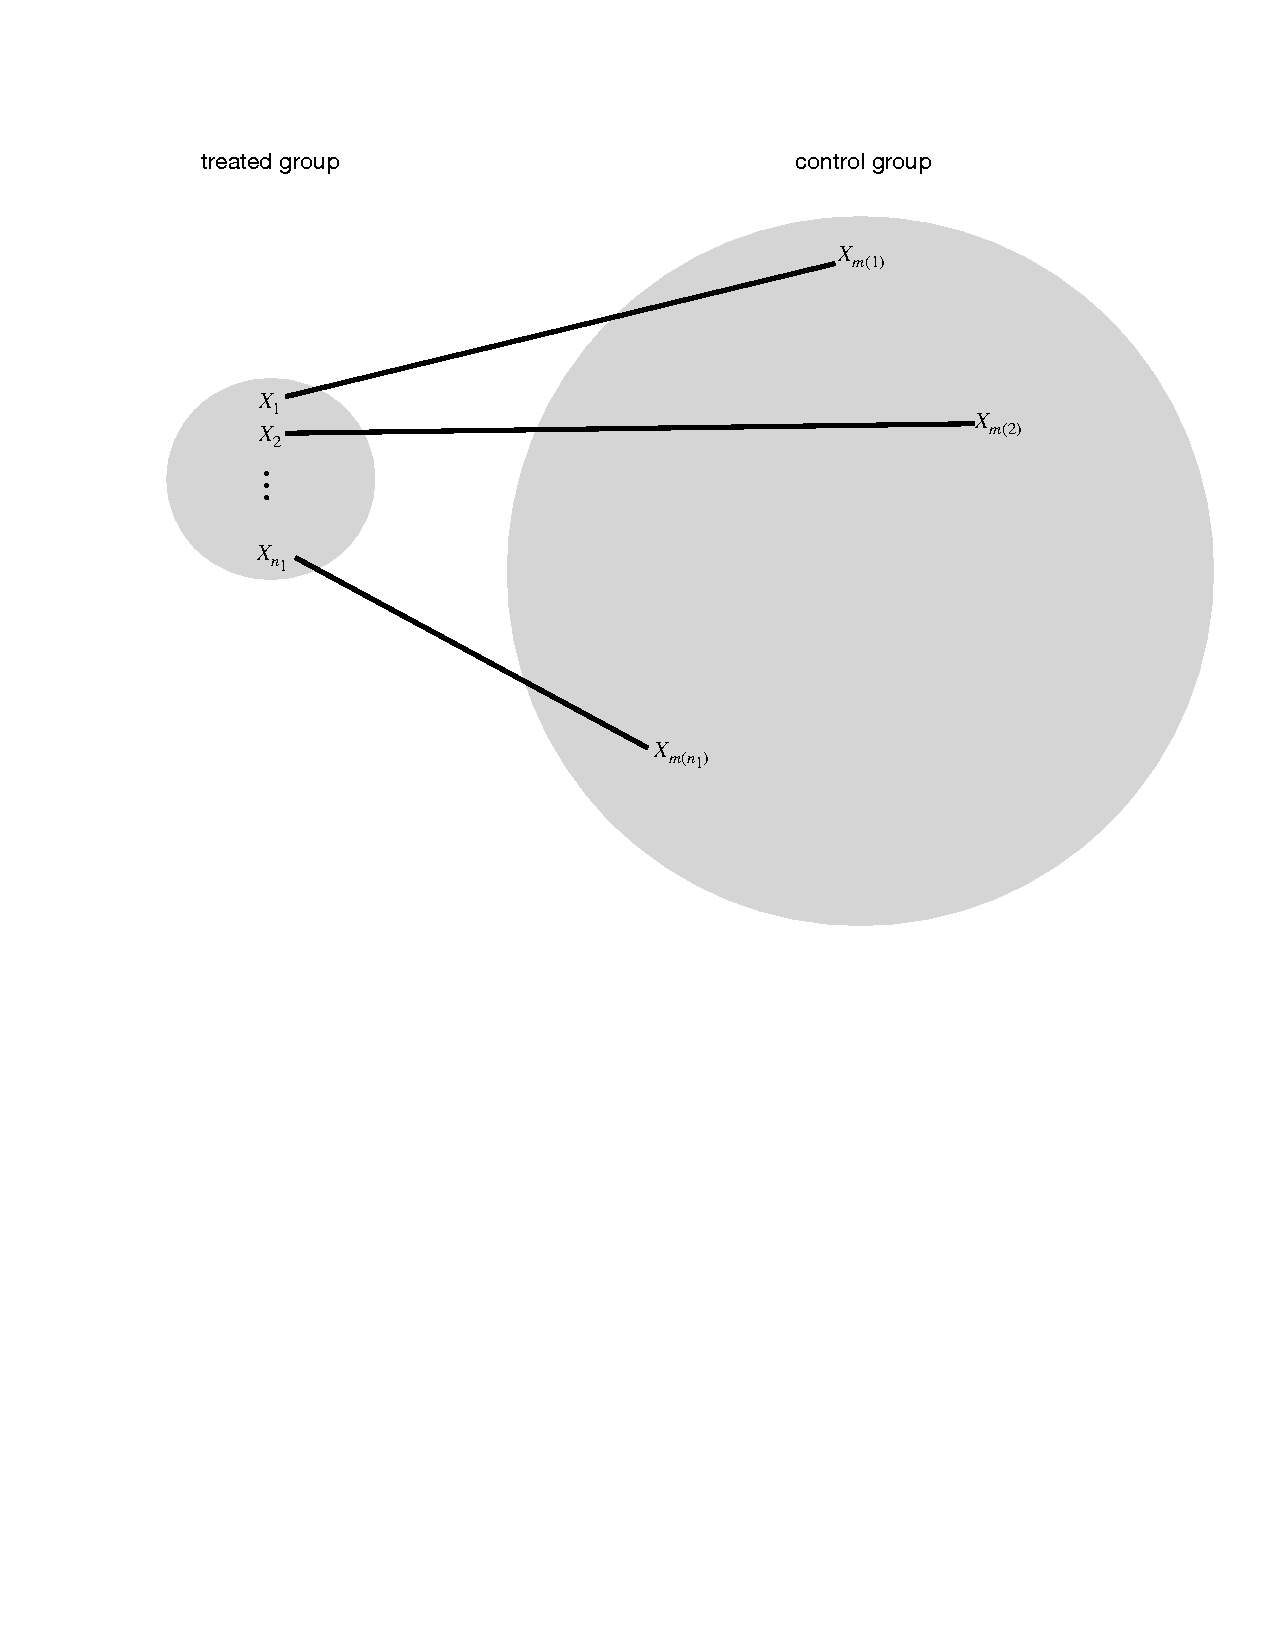
\includegraphics[width = \textwidth]{figures/matchingonetoone.pdf}
\caption{观察性研究中匹配方法的示意图}\label{fig::matching-causal}
\end{figure}


图\ref{fig::matching-causal}展示了处理—对照观察性研究中匹配的基本思想。考虑对照单位数$n_0$远大于处理单位数$ n_1$的简单情形。对处理组中的单位$i=1,\ldots, n_1$，在对照组中找到单位$m(i)$，使$X_i = X_{m(i)}$。理想情况下可以精确匹配，因此每个匹配对内两单位的倾向得分相同，即$e(X_i) = e(X_{m(i)})$。由对称性，在一单位接受处理、另一单位接受对照的条件下，单位$i$接受处理且单位$m(i)$接受对照的概率为$$
\pr( Z_i = 1, Z_{m(i)} = 0 \mid  Z_i +Z_{m(i)} = 1, X_i, X_{m(i)} )  = 1/2
$$\footnote{严格论证如下：\begin{eqnarray*}
&&\pr( Z_i = 1, Z_{m(i)} = 0 \mid  Z_i +Z_{m(i)} = 1, X_i, X_{m(i)} ) \\
&=& \frac{ \pr( Z_i = 1, Z_{m(i)} = 0 \mid   X_i, X_{m(i)} ) }{ \pr( Z_i = 1, Z_{m(i)} = 0 \mid   X_i, X_{m(i)} )   + \pr( Z_i = 0, Z_{m(i)} = 1 \mid   X_i, X_{m(i)} ) } \\
&=& \frac{  e(X_i)  \{ 1 - e(X_{m(i)}) \}  }{ e(X_i)  \{ 1 - e(X_{m(i)}) \}   + \{1-e(X_i)\} e(X_{m(i)}) } \\
&=& \frac{1}{2}.
\end{eqnarray*}}也就是说，给定协变量，并以每对恰有一处理单位和一对照单位为条件，处理分配机制与配对实验相同。因此，可以将精确匹配的观察性研究视为配对实验，用第\ref{chapter::mpe}章的FRT或内曼方法分析，推断已处理单位的因果效应。 


也可以为每个处理单位寻找多个对照单位。一般地，为处理单位$i$找到$M_i$个匹配的对照单位。当各个$M_i$不同时，称为{\it 变比例匹配}\citep{ming2000substantial, ming2001note, pimentel2015variable}。若匹配完全精确，处理分配机制就与第\ref{sec::general-matched-experiment}节讨论的一般匹配实验相同，可以用该节的解析结果分析匹配后的观察性研究。 


\citet{rosenbaum2002design}倡导了上述分析思路。然而在多数观察性研究中，$X_i = X_{m(i)}$这个条件往往无法满足所有单位。此时前述FRT分析逻辑不再成立。最近，\citet{guo2022statistical}指出了不完全匹配情形下FRT方法存在的负面效应，这也为该分析策略敲响了警钟。 
 


\section{更为复杂但更现实的情形}

即便对照组单位数量众多，我们也往往难以实现完全匹配。此时我们只能保证在某种距离度量下$X_i \approx X_{m(i)}  $或$X_i -X_{m(i)} $的值较小。也就是说我们只能获得近似匹配结果。例如，我们可定义
$$
m(i) = \arg\min_{k:Z_k = 0} d(X_i ,X_k), 
$$
其中$d(X_i ,X_k)$表示$X_i$与$X_k$之间的距离。常见的距离度量方式包括欧几里得距离
$$
d(X_i ,X_k) =  (X_i - X_k)\tran ( X_i - X_k),
$$
以及马氏距离
%\footnote{We define $\|v\|_2^2 = \sum_{j=1}^p v_j^2$ for a vector $v = (v_1, \ldots, v_p)\tran$. It denotes the squared length of the vector $v$.}
$$
d(X_i ,X_k) =(X_i - X_k)\tran \Omega^{-1} (X_i - X_k)
$$
此处$\Omega$为总体或对照组单位$X_i$的样本协方差矩阵。 


下文将探讨与匹配方法相关的若干细节问题。相关综述文献可参见\citet{stuart2010matching}。 
\begin{enumerate}
\item
（一对一或一对$M$匹配）
前述讨论均基于一对一匹配方式，上述逻辑亦可推广至一对$M$匹配情形。


\item
本文主要讨论有放回匹配方式，但也有研究者偏好无放回匹配。当对照组单位数量庞大时，这两种方式对最终分析结果的影响通常不大。有放回匹配计算方便，但无放回匹配则涉及复杂的离散最优化计算。有放回匹配所得匹配对质量通常更高，然而因同一单位可能多次参与匹配而带来单位间相关性问题。反之，无放回匹配的优势在于匹配单位间相互独立且后续数据分析更为简便。 


\item
由于匹配过程中配对单位间仍可能存在协变量不均衡问题，因此数据分析时必须进行协变量调整。此时协变量调整不仅为提升估计效率，更是为了纠正潜在偏差。

\item
如果$X$是高维的，那么可能对某个处理单位$i$而言，无论选择哪个对照单位，$d(X_i ,X_k)$都过大。此时可能不得不舍弃一些难以匹配的单位。这样做实际上改变了研究所针对的总体。  


\item
上述问题很难避免。例如，若$X_i \sim \text{N}(0, I_p), X_k \sim\text{N}(0, I_p) ,$且$X_i \ind X_k$，则$$
(X_i - X_k)\tran (X_i - X_k) \sim    2 \chi^2_p
$$其均值为$2p$、方差为$8p$，见第\ref{subsection::chi2-t-distribution}章。理论表明，$p$较大时，不精确匹配会使因果效应估计产生较大偏差。因此，若$p$较大，应在匹配前进行降维。\citet{rosenbaum1983central}提出根据倾向得分匹配。利用估计倾向得分，寻找单位对$\{ i, m(i)\}$，使$ |  \hat{e}(X_i) -  \hat{e}(X_{m(i)})  |$或$| \logit\{ \hat{e}(X_i)\} - \logit\{ \hat{e}(X_{m(i)}) \} | $较小\footnote{定义$\logit(w) = \log \frac{w}{1-w}$。logit函数将$(0,1)$映射到$(-\infty, \infty)$。}，从而将问题化为一维匹配。 
\end{enumerate}

 

\section{平均因果效应的匹配估计量}

Abadie与Imbens（简称AI）通过一系列研究严谨地刻画了匹配估计量的渐近特性，并提出了针对平均因果效应的大样本置信区间计算方法。
他们的研究以观察性研究的经典模型为基准，即$\{ X_i , Z_i ,Y_i(1), Y_i(0)  \}_{i=1}^n \iidsim \{ X, Z, Y(1), Y(0) \}$。  

\subsection{点估计与偏差校正}

AI主要研究有放回的$1$对$M$匹配。对于处理单位$i$，处理下的潜在结果直接插补为$\hat{Y}_i(1) = Y_i$，对照下的潜在结果则插补为$$
\hat{Y}_i(0) = M^{-1} \sum_{k\in J_i} Y_k,
$$其中$J_i$是单位$i$在对照组中的匹配单位集合。例如，可以对所有对照单位$k$计算$d(X_i, X_k)$，再将$J_i$定义为使$d(X_i, X_k)$取最小$M$个值的单位$k$的下标集合。 




对于对照单位$i$，对照下的潜在结果直接插补为$\hat{Y}_i(0) = Y_i$，处理下的潜在结果则插补为$$
\hat{Y}_i(1) = M^{-1} \sum_{k\in J_i} Y_k,
$$其中$J_i$是单位$i$在处理组中的匹配单位集合。

最终匹配估计量定义为
$$
\hat{\tau}^\textup{m} = n^{-1} \sumn \{\hat{Y}_i(1) -\hat{Y}_i(0) \}.
$$

AI证明，$\hat{\tau}^\textup{m}$的偏差不可忽略，尤其是在$X$为多维、且对照单位数与处理单位数相近时。经过技术推导，他们提出以下偏差估计量：$$
\hat{B} = n^{-1} \sumn  \hat{B}_i
$$其中$$
\hat{B}_i = (2Z_i - 1) M^{-1} \sum_{k\in J_i} \{  \hat{\mu}_{1-Z_i}(X_i) -  \hat{\mu}_{1-Z_i}(X_k)     \}
$$$\{  \hat{\mu}_1(X_i), \hat{\mu}_0(X_i) \}$为例如通过OLS拟合得到的结果预测值。对于满足$Z_i  =1$的处理单位，估计偏差为$$
\hat{B}_i = M^{-1} \sum_{k\in J_i} \{  \hat{\mu}_{0}(X_i) -  \hat{\mu}_{0}(X_k)     \}
$$用于修正协变量不匹配导致的对照潜在结果预测差异；对于满足$Z_i = 0$的对照单位，估计偏差为$$
\hat{B}_i =  - M^{-1} \sum_{k\in J_i} \{  \hat{\mu}_{1}(X_i) -  \hat{\mu}_{1}(X_k)     \}
$$用于修正协变量不匹配导致的处理潜在结果预测差异。 


最终经偏差校正后的匹配估计量为
$$
\hat{\tau}^\textup{mbc} = \hat{\tau}^\textup{m}  - \hat{B},
$$
它具有如下线性展开形式。
 
 \begin{proposition}
 \label{prop::matching-expansion-ate} 我们有 
\begin{eqnarray}\label{eq::linearATE}
\hat{\tau}^\textup{mbc}  
= n^{-1} \sumn \hat{\psi}_i
\end{eqnarray} 
其中 
$$
  \hat{\psi}_i = \hat{\mu}_1(X_i) -  \hat{\mu}_0(X_i) + (2Z_i - 1) (1+K_i/M) \{   Y_i - \hat{\mu}_{Z_i}(X_i)  \}
 $$
$K_i$为单位$i$被选作匹配对象的次数。 
 \end{proposition}
 
 
 
命题\ref{prop::matching-expansion-ate}中的线性展开可以通过简单但繁琐的代数运算得到，其证明留作习题\ref{para::linear-bcm-ate}。将$\hat{\tau}^\textup{mbc}  $看作各$  \hat{\psi}_i $的样本均值，便可由线性展开得到简单的方差估计量$$
\hat{V}^\textup{mbc}  = \frac{1}{n^2} \sumn (  \hat{\psi}_i - \hat{\tau}^\textup{mbc}  )^2,
$$\citet{abadie2008failure}首先指出，对原始数据直接进行重抽样的普通自助法不能正确估计匹配估计量的方差，但他们提出的方差估计程序不易实现。\citet{otsu2017bootstrap}提出对线性展开中的$  \hat{\psi}_i $进行自助抽样。然而，\citet{otsu2017bootstrap}的自助法实质上给出的就是易于计算的方差估计量$\hat{V}^\textup{mbc}  $。 


 
\subsection{与双重稳健估计量的关系}
 \label{sec::connection-dr-att}
 
偏差修正匹配估计量与双重稳健估计量密切相关。两者都是在结果回归估计量上，根据残差作某种修正：$$ 
 \hat{R}_i = 
 \begin{cases}
 Y_i - \hat{\mu}_1(X_i)  & \text{ if } Z_i=1;\\
 Y_i - \hat{\mu}_0(X_i)    & \text{ if } Z_i=0.
\end{cases} 
 $$对于平均因果效应$\tau$，回顾结果回归估计量$$
\hat{\tau}^{\textup{reg}} =  n^{-1} \sumn \{ \hat{\mu}_1(X_i) -  \hat{\mu}_0(X_i)\} 
$$和双重稳健估计量$$
\hat{\tau}^\textup{dr}  =  \hat{\tau}^{\textup{reg}} 
+ n^{-1} \sumn \left\{  \frac{Z_i \hat{R}_i }{ \hat{e}(X_i)} -  \frac{ (1-Z_i) \hat{R}_i}{ 1-  \hat{e}(X_i) } \right\} .
$$进一步可以验证，$\hat{\tau}^\textup{mbc} $具有与$\hat{\tau}^\textup{dr}  $相似的形式。
\begin{proposition}
\label{prop::mbc-dr}
经偏差校正后的$\tau$匹配估计量可表示为
$$
\hat{\tau}^\textup{mbc}   =\hat{\tau}^{\textup{reg}} 
+ n^{-1} \sumn \left\{ \left(1+{ K_i\over M} \right)  Z_i \hat{R}_i  - \left( 1+{ K_i\over M} \right) (1-Z_i)  \hat{R}_i \right\} .
$$
\end{proposition}

命题\ref{prop::mbc-dr}的证明留作习题\ref{para::dr-mbc-form}。由命题\ref{prop::mbc-dr}可将匹配看作估计倾向得分的一种非参数方法，并将相应的偏差修正匹配估计量看作双重稳健估计量。例如，$1+K_i /  M$应接近$1/\hat{e}(X_i)$。若某处理单位的$e(X_i)$较小，则基于估计倾向得分的权重$1/\hat{e}(X_i)$较大；同时，它会与很多对照单位匹配，使$K_i$以及$1+K_i /  M$也较大。不过，这种联系也引出了一个明显的问题：当$M$固定时，用$1+K_i /  M$估计$1/e(X_i)$的噪声很大。允许$M$随样本量增大，有望改善基于匹配的倾向得分非参数估计，进而改善匹配及偏差修正匹配估计量的渐近性质。\citet{lin2023estimation}给出了严格理论：只要$M$按适当速率增长，偏差修正匹配估计量$\hat{\tau}^\textup{mbc}   $就能达到与双重稳健估计量相似的性质。  


 
 
 \section{平均治疗效应匹配估计量的推导}

 
对于已处理单位的平均因果效应$$
\tau_\textsc{T} = E(Y\mid Z=1) - E\{  Y(0)  \mid Z=1\},
$$只需为所有处理单位插补缺失的对照潜在结果，即得估计量$$
\hat{\tau}_\textsc{T}^\textup{m} = n_1^{-1} \sumn Z_i \{  Y_i - \hat{Y}_i(0) \}.
$$当$X$为多维时，它同样存在偏差。\citet{otsu2017bootstrap}提出以下偏差估计量：$$  
\hat{B}_\textsc{T} = n_1^{-1} \sumn Z_i  \hat{B}_{\textsc{T},i} 
$$其中$$
\hat{B}_{\textsc{T},i} = M^{-1} \sum_{k \in J_i} \{  \hat{\mu}_0(X_i) -  \hat{\mu}_0(X_k)     \}
$$用于修正满足$Z_i = 1.$的处理单位因协变量不匹配而产生的偏差。


最终经偏差校正后的估计量为：
$$
\hat{\tau}_\textsc{T}^\textup{mbc} = \hat{\tau}_\textsc{T}^\textup{m} - \hat{B}_\textsc{T},
$$ 
其具有如下线性展开形式。

\begin{proposition}\label{prop::linear-expansion-att}
我们有 
\begin{eqnarray}\label{eq::linearATT}
\hat{\tau}_\textsc{T}^\textup{mbc}  =   n_1^{-1} \sumn \hat{\psi}_{\textsc{T}, i},
\end{eqnarray}
其中 
$$
\hat{\psi}_{\textsc{T}, i} =   Z_i \{ Y_i - \hat{\mu}_0(X_i) \}
- (1-Z_i) K_i/M \{ Y_i - \hat{\mu}_0(X_i) \} . 
$$
\end{proposition}

证明留作习题\ref{para::linear-bcm-ate}。受\citet{otsu2017bootstrap}启发，可以将$\hat{\tau}_\textsc{T}^\textup{mbc}  $看作$n/n_1$与各$\hat{\psi}_{\textsc{T}, i}$样本均值的乘积，因此一个直观的方差估计量为$$
\hat{V}_\textsc{T}^\textup{mbc} =  \left( \frac{n}{n_1} \right)^2 \frac{1}{n^2} \sumn (\hat{\psi}_{\textsc{T}, i} - \hat{\tau}_\textsc{T}^\textup{mbc} n_1/n)^2 = \frac{1}{n_1^2} \sumn (\hat{\psi}_{\textsc{T}, i} - \hat{\tau}_\textsc{T}^\textup{mbc} n_1/n )^2.
$$

 
 与第\ref{sec::connection-dr-att}节的讨论类似，可以将双重稳健估计量和偏差修正匹配估计量与结果回归估计量进行比较。对于已处理单位的平均因果效应$\tau_\textsc{T}$，回顾结果回归估计量$$
\hat{\tau}^{\textup{reg}}_\textsc{T} = n_1^{-1} \sumn Z_i \{ Y_i - \hat{\mu}_0(X_i) \} ,
$$和双重稳健估计量$$
\hat{\tau}_\textsc{T}^\textup{dr} =  \hat{\tau}^{\textup{reg}}_\textsc{T} 
- n_1^{-1} \sumn \frac{  \hat{e}(X_i) }{ 1- \hat{e}(X_i) }  (1-Z_i)  \hat{R}_i .
$$进一步可以验证，$\hat{\tau}_\textsc{T}^\textup{mbc} $具有与$\hat{\tau}_\textsc{T}^\textup{dr} $相似的形式。 
\begin{proposition}
\label{prop::mbc-dr-att}
经偏差校正后的$\tau_\textsc{T}$匹配估计量可表示为
$$
\hat{\tau}_\textsc{T}^\textup{mbc}   = \hat{\tau}^{\textup{reg}}_\textsc{T} 
 - n_1^{-1} \sumn { K_i\over M}  (1-Z_i)  \hat{R}_i.
$$
\end{proposition}


命题\ref{prop::mbc-dr-att}的证明留作习题\ref{para::dr-mbc-form-att}。命题\ref{prop::mbc-dr-att}表明，匹配实质上是用$K_i/M$估计给定协变量时接受处理的优势。 




\section{实例分析}
\label{sec::matching-application}



\subsection{实验数据}
现在使用\citet{sekhon2011multivariate}的\ri{Matching}包重新分析LaLonde数据。此前已多次使用该包中的\ri{lalonde}数据集，这里将使用其核心函数\ri{Match}。实验部分得到以下结果：
\begin{lstlisting}
> library("car")
> library("Matching")
> 
> ## Chapter 15.5.1
> ## experimental data
> data("lalonde")
> y = lalonde$re78
> z = lalonde$treat
> x = as.matrix(lalonde[, c("age", "educ", "black",
+                           "hisp", "married", "nodegr",
+                           "re74", "re75")])
> 
> ## analysis the randomized experiment
> neymanols = lm(y ~ z)
> fisherols = lm(y ~ z + x)
> xc = scale(x)
> linols = lm(y ~ z*xc)
> resols = c(neymanols$coef[2],
+            fisherols$coef[2],
+            linols$coef[2],
+            sqrt(hccm(neymanols, type = "hc2")[2, 2]),
+            sqrt(hccm(fisherols, type = "hc2")[2, 2]),
+            sqrt(hccm(linols, type = "hc2")[2, 2]))
> resols = matrix(resols, 3, 2)
> rownames(resols) = c("neyman", "fisher", "lin")
> colnames(resols) = c("est", "se")
> resols 
            est       se
neyman 1794.343 670.9967
fisher 1676.343 677.0493
lin    1621.584 694.7217
\end{lstlisting} 
各回归估计量均显示职业培训项目具有显著正向效应。若采用一对一匹配方式分析该实验数据，可得：
\begin{lstlisting}
> matchest.adj = Match(Y = y, Tr = z, X = x, BiasAdjust = TRUE)
> summary(matchest.adj)

Estimate...  2119.7 
AI SE......  876.42 
T-stat.....  2.4185 
p.val......  0.015583 

Original number of observations..............  445 
Original number of treated obs...............  185 
Matched number of observations...............  185 
Matched number of observations  (unweighted).  268
\end{lstlisting} 
估计值与标准误虽有所上升，但结论未发生改变。 


\subsection{观察性数据}
接着重新分析与上述实验相对应的观察性数据：
\begin{lstlisting}
> dat <- read.table("cps1re74.csv", header = TRUE)
> dat$u74 <- as.numeric(dat$re74==0)
> dat$u75 <- as.numeric(dat$re75==0)
> y = dat$re78
> z = dat$treat
> x = as.matrix(dat[, c("age", "educ", "black",
+                           "hispan", "married", "nodegree",
+                           "re74", "re75", "u74", "u75")])
 \end{lstlisting} 
然而采用一对一匹配方式后可得接近实验基准值的估计结果：
\begin{lstlisting}
> neymanols = lm(y ~ z)
> fisherols = lm(y ~ z + x)
> xc = scale(x)
> linols = lm(y ~ z*xc)
> resols = c(neymanols$coef[2],
+            fisherols$coef[2],
+            linols$coef[2],
+            sqrt(hccm(neymanols, type = "hc2")[2, 2]),
+            sqrt(hccm(fisherols, type = "hc2")[2, 2]),
+            sqrt(hccm(linols, type = "hc2")[2, 2]))
> resols = matrix(resols, 3, 2)
> rownames(resols) = c("neyman", "fisher", "lin")
> colnames(resols) = c("est", "se")
> resols 
             est        se
neyman -8506.495  583.4426
fisher  1067.546  628.4389
lin    -4265.801 3211.7718
  \end{lstlisting} 
  忽略匹配结果中的重复单位问题，采用配对分析方法可得到类似实验数据的结果：
  \begin{lstlisting}
> matchest = Match(Y = y, Tr = z, X = x, BiasAdjust = TRUE)
> summary(matchest)

Estimate...  1747.8 
AI SE......  916.59 
T-stat.....  1.9068 
p.val......  0.056543 

Original number of observations..............  16177 
Original number of treated obs...............  185 
Matched number of observations...............  185 
Matched number of observations  (unweighted).  248
   \end{lstlisting} 
   
忽略匹配数据中的并列匹配，还可以使用配对分析，其结果同样与实验数据的结果相近：
  \begin{lstlisting}
> diff = y[matchest$index.treated] - 
+           y[matchest$index.control]
> round(summary(lm(diff ~ 1))$coef[1, ], 2)
  Estimate Std. Error    t value   Pr(>|t|) 
   1581.44     558.55       2.83       0.01 
> 
> diff.x = x[matchest$index.treated, ] - 
+               x[matchest$index.control, ]
> round(summary(lm(diff ~ diff.x))$coef[1, ], 2)
  Estimate Std. Error    t value   Pr(>|t|) 
   1842.06     578.37       3.18       0.00 
   \end{lstlisting} 
   
   
   
   \subsection{协变量均衡性检验}
   
我们还可通过简单OLS检验匹配前后协变量分布。匹配前协变量存在严重不均衡性，具体表现为大量回归系数带有显著性标记。 
  \begin{lstlisting}
> lm.before = lm(z ~ x)
> summary(lm.before) 

Residuals:
     Min       1Q   Median       3Q      Max 
-0.18508 -0.01057  0.00303  0.01018  1.01355 

Coefficients:
              Estimate Std. Error t value Pr(>|t|)    
(Intercept)  1.404e-03  6.326e-03   0.222   0.8243    
xage        -4.043e-04  8.512e-05  -4.750 2.05e-06 ***
xeduc        3.220e-04  4.073e-04   0.790   0.4293    
xblack       1.070e-01  2.902e-03  36.871  < 2e-16 ***
xhispan      6.377e-03  3.103e-03   2.055   0.0399 *  
xmarried    -1.525e-02  2.023e-03  -7.537 5.06e-14 ***
xnodegree    1.345e-02  2.523e-03   5.331 9.89e-08 ***
xre74        7.601e-07  1.806e-07   4.208 2.59e-05 ***
xre75       -1.231e-07  1.829e-07  -0.673   0.5011    
xu74         4.224e-02  3.271e-03  12.914  < 2e-16 ***
xu75         2.424e-02  3.399e-03   7.133 1.02e-12 *** 
      \end{lstlisting} 
      
      
      匹配后所有回归系数均不再具有显著性标记，表明协变量分布已显著均衡。 
      
      
   \begin{lstlisting}
> lm.after = lm(z ~ x, 
+               subset = c(matchest$index.treated, 
+                          matchest$index.control))
> summary(lm.after) 

Residuals:
     Min       1Q   Median       3Q      Max 
-0.66864 -0.49161 -0.03679  0.50378  0.65122 

Coefficients:
              Estimate Std. Error t value Pr(>|t|)  
(Intercept)  6.003e-01  2.427e-01   2.474   0.0137 *
xage         3.199e-03  3.427e-03   0.933   0.3511  
xeduc       -1.501e-02  1.634e-02  -0.918   0.3590  
xblack       6.141e-05  7.408e-02   0.001   0.9993  
xhispan      1.391e-02  1.208e-01   0.115   0.9084  
xmarried    -1.328e-02  6.729e-02  -0.197   0.8437  
xnodegree   -3.023e-02  7.144e-02  -0.423   0.6723  
xre74        6.754e-06  9.864e-06   0.685   0.4939  
xre75       -9.848e-06  1.279e-05  -0.770   0.4417  
xu74         2.179e-02  1.027e-01   0.212   0.8321  
xu75        -2.642e-02  8.327e-02  -0.317   0.7512
         \end{lstlisting} 
         
         

\section{讨论}


当协变量数量较多时，直接基于原始变量进行匹配可能会受到维数灾难影响。\citet{rosenbaum1983central}建议改用基于倾向性得分的匹配方式。\citet{abadie2016matching}为此策略奠定了理论基础。 
         
         
         
\section{作业习题}

\paragraph{偏差校正估计量的线性展开}\label{para::linear-bcm-ate}


 证明命题 \ref{prop::matching-expansion-ate} 和 \ref{prop::linear-expansion-att}。 
 
 
 
\paragraph{$\tau$的偏差校正匹配估计量的双重稳健形式}\label{para::dr-mbc-form}

证明命题\ref{prop::mbc-dr}。  


\paragraph{$\tau_\textsc{t}$的偏差修正匹配估计量的双重稳健形式}\label{para::dr-mbc-form-att}

证明命题\ref{prop::mbc-dr-att}。  
 

\paragraph{重审实例\ref{eg::chan-bmi-ATE}}


运用匹配估计量分析实例\ref{eg::chan-bmi-ATE}中的数据集，并比较所得结论与其他方法的差异。分析时应检验匹配前后协变量的均衡性，可尝试不同匹配数目设定，甚至可在匹配后应用多种估计方法。结论是否受参数选择影响？ 

 


\paragraph{重审第\ref{sec::matching-application}节内容}


第\ref{sec::matching-application}章使用匹配分析了LaLonde观察性研究。匹配表现良好，因为其估计结果接近作为金标准的实验结果。用结果回归、倾向得分分层、两种IPW估计量和双重稳健估计量重新分析这些数据，将结果与匹配估计量及实验金标准估计量比较。

该节采用匹配方法分析LaLonde观察性研究，所得结果接近实验基准值。现请分别运用结果回归、倾向性得分分层、两种逆概率加权及双重稳健估计方法重新分析该数据。将各方法结果相互比较并与实验基准值对照。 

注意：实验设计允许各类参数自定义。例如分层数、倾向性得分截断阈值、回归模型形式等。亦可尝试将匹配方法应用于匹配后数据集。该数据集已被大量研究采用，相关文献可参考\citep{dehejia1999causal, hainmueller2012entropy}，同时鼓励开展创新性分析。



\paragraph{数据再分析}

\citet{ho2007matching}是政治学领域一篇有影响力的论文，作者据此开发了\ri{R}包\ri{MatchIt}\citep{ho2011matchit}。\citet{ho2007matching}分析了两个数据集，均可从Harvard Dataverse获取。

请运用本文所述方法重新分析该两组数据，亦可尝试其他合理方法。 


 \paragraph{推荐阅读}
 
匹配估计量相关文献浩繁，推荐阅读三篇权威综述\citet{sekhon2009opiates}, \citet{stuart2010matching}, \citet{imbens2015matching}。 


 

 
  
  
\part{观察性研究的困难与挑战}\label{part::challenges-os}  
  
  
\chapter{观察性研究中存在未混杂假设时的困难}
 \label{chapter::difficulties-observational-studies}
 
 
本书的\ref{part::observational-studies}部分探讨了在两个假设之下利用观察性研究进行因果推断的方法：未混杂假设与重叠假设。这两个假设均属于较强的假设，实践中往往难以满足。本章将着重讨论未混杂假设的困难之处。随后的\ref{chapter::evalue}--\ref{sec::rosenbaum-sensitivity-analysis}各章将介绍在存在未测量混杂因素的情况下，观察性研究中进行敏感性分析的各种策略。\ref{chapter::overlap}章则将探讨重叠假设的困难。 
 
 
 

\section{因果图的基本概念}


\citet{pearl1995causal}率先引入了因果图这一概念，将其作为实证研究中进行因果推断的有力工具。\citet{pearl2000causality}则撰写了关于因果图的教科书。在此，我也将因果图视作一种直观描述变量间因果关系的工具。 

例如，考虑以下因果图$$
\xymatrix{
 & X \ar[ld]\ar[rd] \\
Z\ar[rr] &&Y 
}
$$研究$Z$对$Y$的因果效应时，可以将它解读为如下数据生成过程：$$
\left\{ 
\begin{aligned}
      X & \sim F_X(x), \\
      Z  &=   f_Z(X, \varepsilon_Z) , \\
      Y(z) &=  f_Y(X, z, \varepsilon_Y(z)) ,
\end{aligned}
\right. 
$$其中对$z=0,1$均有$\varepsilon_Z \ind \varepsilon_Y(z)$。在这里，协变量$X$来自分布$F_X(x)$，处理分配是$X$和随机误差项$\varepsilon_Z$的函数，潜在结果$ Y(z) $是$X$、$z$和随机误差项$\varepsilon_Y(z)$的函数。由这些方程容易看出$Z\ind Y(z) \mid X$，即无混杂性假设成立。 


若因果图为$$
\xymatrix{
 X \ar[d]\ar[rrd] & & U\ar[d]\ar[lld] \\
Z\ar[rr] &&Y 
}
$$可将其解读为如下数据生成过程：$$
\left\{ 
\begin{aligned}
       X & \sim F_X(x), \\
       U& \sim F_U(u), \\ 
      Z  &=   f_Z(X, U,  \varepsilon_Z) , \\
      Y(z) &=  f_Y(X, U, z, \varepsilon_Y(z)) ,
\end{aligned}
\right. 
$$其中对$z=0,1$均有$\varepsilon_Z \ind \varepsilon_Y(z)$。由方程容易看出$Z\ind Y(z) \mid (X,U)$，但$Z\nind Y(z) \mid X$，即以$(X,U)$为条件时无混杂性成立，而仅以$X$为条件时不成立。此时，$U$是一个未测量混杂因素。图中的$U$因此称为未测量混杂因素。 






\section{评估未混杂假设的方法}


无混杂性假设$$
Z\ind Y(1) \mid X, \quad 
Z\ind Y(0) \mid X
$$蕴含\begin{eqnarray*}
\pr\{ Y(1)\mid  Z=1, X \}  &=& \pr\{ Y(1)\mid  Z=0, X \} , \\
\pr\{ Y(0)\mid  Z=1, X \} &=& \pr\{ Y(0)\mid  Z=0, X \} . 
\end{eqnarray*}因此，它实质上要求反事实分布$\pr\{ Y(1)\mid  Z=0, X \}$等于观测分布$\pr\{ Y(1)\mid  Z=1, X \}$，且反事实分布$\pr\{ Y(0)\mid  Z=1, X \} $等于观测分布$\pr\{ Y(0)\mid  Z=0, X \}$。由于反事实分布不能直接从数据中识别，在没有额外假设时，无混杂性在根本上不可检验。下面讨论评估无混杂性假设的两种策略。这里的“评估”弱于“检验”：前者指支持或削弱初始分析的补充分析，后者指正式的统计检验。 



\subsection{利用负对照结果}


 

设$Y^\textup{n}$是与$Y$相似的结果，理想情况下具有与$Y$相同的混杂结构。若相信$Z\ind Y(z)\mid X$，一般也倾向于相信$Z\ind Y^\textup{n} (z)\mid X$。此外，事先已知$Z$对$Y^\textup{n}$的效应：$$
\tau(Z\rightarrow Y^\textup{n} )
= 
E\{  Y^\textup{n}(1) - Y^\textup{n}(0) \} .
$$一个重要例子是$\tau(Z\rightarrow Y^\textup{n} ) = 0$。满足这些要求的因果图如下：

$$
\xymatrix{
 & X \ar[ld]\ar[rd] \ar[rr] & & Y^\textup{n}  \\
Z\ar[rr] &&Y 
}
$$



\begin{example}
\citet{Cornfield::1959}基于观察性研究探讨了吸烟与肺癌之间的因果关系。尽管他们控制了诸多重要背景变量，但仍可能存在某些未测量的混杂因素影响观测结果。为强化因果关系的证据，他们同时报告了吸烟对车祸发生率的影响——该值在生物学预期范围内应接近零。由此可见，即便无法排除未测量混杂因素的存在，基于负对照结果的辅助分析依然能强化“吸烟导致肺癌”这一结论的可靠性。 
\end{example}

\begin{example}
\citet{imbens2015causal}建议将滞后结果用作负对照结果。在大多数情形下，认为滞后结果与当前结果具有相似的混杂结构是合理的。由于滞后结果发生在处理之前，处理对它的平均因果效应必为$0$。不过应谨慎使用这一建议，因为在大多数研究中，我们会直接将滞后结果作为一个已观测混杂因素进行调整。 

从某种意义上说，第\ref{chapter::pscore-key}章中的协变量平衡检查是使用负对照的一个特例。与将滞后结果用作负对照的问题相似，这些协变量通常已包含在无混杂性假设中。因此，协变量平衡检查未通过，实际上否定的是倾向得分模型的设定，而非无混杂性假设本身。 
\end{example}

\begin{example}
针对老年人的观察性研究发现，在调整已测量协变量后，接种流感疫苗显著降低随后流感季的肺炎或流感住院风险及全因死亡风险。\citet{jackson2006evidence}怀疑这一效应幅度过大，于是对负对照结果进行了补充分析。疫苗通常从秋季开始接种，而流感传播在冬季之前往往很少。根据生物学知识，疫苗效应应在流感季最明显。但\citet{jackson2006evidence}发现在流感季之前效应反而更大，提示观察到的效应来自未测量混杂。 
\end{example}

在上述案例中，\citet{jackson2006evidence}的研究最具说服力：流感相关结果在流感季前后应具有相似的混杂特征。相比之下，\citet{Cornfield::1959}的证据稍弱：吸烟与车祸之间和吸烟与肺癌之间的因果机制存在显著差异。事实上，\citet{Fisher::1957}曾指出吸烟与肺癌的关系可能源于某种未被观测的遗传因素（参见\ref{chapter::evalue}章）。这种因素虽能同时影响吸烟行为与肺癌发病率，却不太可能显著影响车祸发生率。  


\citet{lipsitch2010negative}是近期关于负对照结果研究的代表文献；而\citet{rosenbaum1989role}则探讨了已知效应在因果推断中的作用。 

 

\subsection{利用负对照暴露}

 


负对照暴露与负对照结果相互对应。设$Z^\textup{n}$是与$Z$相似的处理变量，并具有与$Z$相同的混杂结构。若相信$Z \ind Y  (z) \mid X$，通常也倾向于相信$
Z^\textup{n}\ind Y  (z) \mid X.
$。此外，事先已知$Z^\textup{n}$对$Y $的效应$$
\tau(Z^\textup{n}\rightarrow Y  )
= 
E\{  Y(1^\textup{n}) - Y (0^\textup{n}) \}.
$$一个重要例子是$\tau(Z^\textup{n}\rightarrow Y  ) = 0.$。满足这些要求的因果图如下：


$$
\xymatrix{
Z^\textup{n} & & X \ar[ll] \ar[ld]\ar[rd] \\
&Z  \ar[rr] && Y 
}
$$




\begin{example}
\citet{sanderson2017negative}提供了诸多应用负对照暴露的实例：通过比较孕期母体与父亲接触因素各自对子代结局的影响，从而判断子宫内暴露的效应。该文献综述了多项关于父母吸烟、BMI分别对子代发育影响的研究。在此类情境下，母体效应值理论上应大于父亲效应值。 
\end{example}



\subsection{总结}


若无额外假设，未混杂假设本质上无法被检验。尽管观察性研究中的负对照结果或负对照无法直接验证该假设，但将其用于辅助分析却能强化因果推断的可信度。然而实施此类分析并非易事：它往往需要更多数据，更重要的是需深入理解因果机制方能选择合适的负对照指标。 

 
 


\section{过度调整引发的问题}
\label{sec::pearl-bias}

此前讨论的许多因果效应估计方法都依赖无混杂性假设：$$
Z\ind \{ Y(1), Y(0) \} \mid X .
$$这个假设以$X$为条件，因此必须选对$X$，以确保所需的条件独立性。\citet{rosenbaum2002design}认为，没有理由避免调整描述受试者处理前情况的变量。类似地，\citet{rubin2007design}认为，通常假设的条件越充分，就越容易接受。两者都主张控制所有已观测的处理前协变量。\citet{vanderweele2011new}将其称为{\it 处理前准则}。Pearl不同意这一建议，并给出了下面两个反例。 


\subsection{M型偏差}
\label{section::m-bias}

M偏差出现在以下具有M形结构的因果图中：$$
\xymatrix{
U_1 \ar[dd]\ar[dr] &&U_2 \ar[dd]\ar[dl] \\
&X& \\
Z   && Y 
}
$$

由图可读出数据生成过程：$$
\left\{ 
\begin{aligned}
&U_1 \ind U_2 ,\\
&X = f_X(U_1, U_2, \varepsilon_X),\\
&Z=   f_Z(U_1,  \varepsilon_Z) , \\
&Y=      Y(z) =  f_Y(U_2, \varepsilon_Y) ,
\end{aligned}
\right. 
$$其中$(\varepsilon_X, \varepsilon_Z, \varepsilon_Y) $是相互独立的随机误差项。上述图中的$X$已观测，而$U_1$和$U_2$未观测。改变$Z$的值完全不会改变$Y$的值，因此$Z$对$Y$的真实因果效应必为$0$。由数据生成方程可知$Z\ind Y$，因而$Z$与$Y$的关联为$0$；特别地，$$
\tau_\textsc{PF} = E(Y\mid Z=1) - E(Y\mid Z=0) = 0.
$$这意味着，不调整协变量$X$的简单估计量对真实参数是无偏的。 

然而，以$X$为条件后，$U_1\nind  U_2 \mid X$，进而一般有$Z\nind Y\mid X$以及$$
\int \{  E(Y\mid Z=1, X=x) - E(Y\mid Z=0, X=x) \} f(x) \diff x \neq 0
$$为获得直观理解，考虑正态线性模型\footnote{这与二元$Z$的讨论并不完全契合，但可简化推导。\citet{ding2015adjust}对二元$Z$下更自然的模型作了详细讨论。}：$$
\left\{ 
\begin{aligned}
&X = a U_1 + b U_2 +  \varepsilon_X,\\
&Z=   cU_1 +  \varepsilon_Z , \\
&Y=      Y(z) =  dU_2 +  \varepsilon_Y ,
\end{aligned}
\right. 
$$其中$(U_1, U_2, \varepsilon_X, \varepsilon_Z, \varepsilon_Y)  \iidsim \N01$。我们有$$
\cov(Z,Y) = \cov(  cU_1 +  \varepsilon_Z,  dU_2 +  \varepsilon_Y) = 0,
$$但根据习题\ref{hw::partial-correlation}的结果，给定$X$时$Z$与$Y$的偏相关系数为\footnote{符号$\propto$读作“正比于”，使我们可以省略一些不重要的常数。}\begin{eqnarray*}
\rho_{ZY\mid X} &=& \frac{   \rho_{ZY} - \rho_{ZX} \rho_{YX}  }{  \sqrt{  1-\rho_{ZX}^2 }  \sqrt{1- \rho_{YX}^2  }  }   
\\
&\propto &  - \rho_{ZX} \rho_{YX}  \\
&\propto &  - \cov(Z, X) \cov(Y, X)  \\
&=&  - abcd,
\end{eqnarray*}即沿$Z$至$Y$路径上各系数的乘积。因此，未调整的估计量无偏，而调整后的估计量具有正比于$abcd$的偏差。 


 
 
如下简单示例可演示M型偏差：

\begin{lstlisting}
> ## M bias with large sample size
> n  = 10^6
> U1 = rnorm(n)
> U2 = rnorm(n)
> X  = U1 + U2 + rnorm(n)
> Y  = U2 + rnorm(n)
> ## with a continuous treatment Z
> Z  = U1 + rnorm(n)
> round(summary(lm(Y ~ Z))$coef[2, 1], 3)
[1] 0
> round(summary(lm(Y ~ Z + X))$coef[2, 1], 3)
[1] -0.2
> 
> ## with a binary treatment Z
> Z  = (Z >= 0)
> round(summary(lm(Y ~ Z))$coef[2, 1], 3)
[1] 0.002
> round(summary(lm(Y ~ Z + X))$coef[2, 1], 3)
[1] -0.42
\end{lstlisting}



\subsection{Z型偏差}
\label{sec::z-bias}

 

考虑以下因果图$$
\xymatrix{
&&&U \ar[dl]_b \ar[dr]^c \\
X \ar[rr]^a &&Z\ar[rr]^\tau   && Y 
}
$$其数据生成过程为\footnote{这里同样用线性模型生成连续$Z$以简化推导。\citet{ding2017instrumental}将理论推广到更一般的因果模型，特别是二元$Z$的情形。}$$
\left\{ 
\begin{aligned}
&Z=   aX + bU +   \varepsilon_Z , \\
&Y(z)=   \tau z + cU +  \varepsilon_Y ,
\end{aligned}
\right. 
$$其中$(U, X, \varepsilon_Z, \varepsilon_Y) $独立同分布于$ \N01$。在此过程中，$X\ind U,$$X\nind Z$，且$X$仅通过$Z$影响$Y$。  

 
未调整的估计量为\begin{eqnarray*}
\tau_\textup{unadj} &=& \frac{ \cov(Z, Y)  }{  \var(Z) }  \\
&=& \frac{ \cov(Z, \tau Z + cU)  }{ \var(Z) }  \\
&=& \tau + \frac{c \cov(aX + bU, U)  }{  \var(Z) }  \\
&=& \tau + \frac{c b }{  a^2 + b^2 + 1} ,
\end{eqnarray*}其偏差为$bc/(a^2 + b^2 + 1)$。将$Y$对$(Z,X)$进行OLS回归得到的调整估计量满足$$
\left\{ 
\begin{aligned}
E\{  Z(Y- \tau_\textup{adj} Z  - \alpha X  )  \} &= 0,\\
E\{  X(Y - \tau_\textup{adj} Z - \alpha X)  \} &= 0.
\end{aligned}
\right. 
$$解这个关于$(\tau_\textup{adj}, \alpha)$的线性方程组，得到$  \tau_\textup{adj}$的表达式：\begin{equation}
\label{eq::zbias-result}
  \tau_\textup{adj}  = \tau +  \frac{    bc }{   b^2+1 },
\end{equation}其偏差为$bc/(b^2+1)$。求解关于$(\tau_\textup{adj}, \alpha)$的方程组的具体步骤留作习题\ref{hw::z-bias-formula}。 

由此可见未调整估计量的偏差小于调整后结果。更值得注意者：当$X$与$Z$关联越强（$a$值越大），调整后偏差反而越大。 


数学推导并不十分困难，但这种偏差似乎颇为反直觉。直观解释如下：处理是$X$、$U$及其他随机误差的函数。给定$X$后，它便仅是$U$和其他随机误差的函数。因此，以$X$为条件会降低$Z$的随机性，更关键的是，会增大未测量混杂因素$U$在决定$Z$时的相对作用。于是，以$X$为条件会放大$U$造成的混杂偏差。这个理想化例子说明了对某些协变量过度调整的危险。 



 \citet{heckman2004using}在模拟研究中观察到这一现象；\citet[][technical report in 2006]{wooldridge2009should}在线性模型中验证了它；\citet{pearl2010class, pearl2011invited}用因果图作出解释；\citet{ding2017instrumental}提供了更一般的理论和直观解释。它被称为Z偏差，是因为Pearl的原始论文用符号$Z$表示这里的变量$X$。但本书始终用$Z$表示处理变量。在本书第\ref{part::instrumentalvariables}部分中，满足本小节因果图条件的$X$称为工具变量。因此，这种偏差也称为{\it 工具变量偏差}。 



如下示例能直观演示Z型偏差：
\begin{lstlisting}
> ## Z bias with large sample size
> n  = 10^6
> X = rnorm(n)
> U = rnorm(n)
> Z = X + U + rnorm(n)
> Y = U + rnorm(n)
> 
> round(summary(lm(Y ~ Z))$coef[2, 1], 3)
[1] 0.333
> round(summary(lm(Y ~ Z + X))$coef[2, 1], 3)
[1] 0.501
> 
> ## stronger association between X and Z
> Z = 2*X + U + rnorm(n)
> round(summary(lm(Y ~ Z))$coef[2, 1], 3)
[1] 0.167
> round(summary(lm(Y ~ Z + X))$coef[2, 1], 3)
[1] 0.501
> 
> ## even stronger association between X and Z
> Z = 10*X + U + rnorm(n)
> round(summary(lm(Y ~ Z))$coef[2, 1], 3)
[1] 0.01
> round(summary(lm(Y ~ Z + X))$coef[2, 1], 3)
[1] 0.5
\end{lstlisting} 


\subsection{观察性研究中该调整哪些协变量？}


真实的数据生成过程可能十分复杂，我们无法确知。不过，下面的因果图有助于厘清许多概念。它已经排除了第\ref{section::m-bias}节讨论的$M$偏差：$$
\xymatrix{
 &&X_R&& \\
X_Z \ar[ddr] && X \ar[ddl] \ar[ddr]&& X_Y \ar[ddl] \\
 &\\
 &Z \ar[rr] \ar[ddr] &&Y \ar[ddl]& \\
 & \\
 &&X_I&&
}
$$图中各协变量具有不同特征： 
\begin{enumerate}
\item
$X$同时影响处理和结果。以$X$为条件可以确保无混杂性，因此应控制$X$。
\item
$X_R$为纯随机噪声因素，不影响处理与结果。纳入此类变量虽不致偏差估计，却会增加有限样本下的变异度。
\item
$X_Z$是仅通过处理影响结果的工具变量。在上图中，将其纳入分析不会使估计有偏，但会增大估计的变异性。然而，存在未测量混杂时，将其纳入分析会放大偏差，如第\ref{sec::z-bias}节所示。 
\item
$X_Y$仅影响结果而与处理无关。不调整条件下未混杂假设仍成立。因其具预测结果之效，纳入分析常可提升估计精度。
\item
$X_I$受处理与结果共同影响，属处理后变量而非处理前协变量。若目标是推断处理效应则不应纳入。关于处理后变量的因果推断问题将在\ref{part::post-treatmentvariable}部分详述。 
\end{enumerate}



若认可上述因果结构，则至少需调整$X$以消除偏差；若可能，还应纳入$X_Y$以降低变异度。 


 
 
 
\section{作业习题}


\paragraph{Z型偏差公式推导细节}\label{hw::z-bias-formula}
请验证公式\eqref{eq::zbias-result}的正确性。
 

\paragraph{Cochran公式与遗漏变量偏差公式}
\label{hw::cochran+ovb}



David Cox爵士将以下结果称为{\it Cochran公式}\citep{cochran1938omission, cox2007generalization}，计量经济学家则称其为{\it 遗漏变量偏差公式}\citep{angrist2008mostly}。\citet{fisher1925statistical}已给出其中一个特例。它也对应于第\ref{appendix::fwl-theorem}章中的Frisch–Waugh–Lovell定理。  

该公式分两个版本。下述向量均为列向量： 

\begin{enumerate}
[(1)]
\item
（总体版本）设$(y_i, x_{1i}, x_{2i})_{i=1}^n$独立同分布，其中$y_i$为标量，$x_{i1}$为$K$维向量，$x_{i2}$为$L$维向量。 

对这些随机变量作如下OLS分解：\begin{eqnarray}
y_i &=& \beta_1 \tran x_{i1} + \beta_2  \tran x_{2i} + \varepsilon_i , \label{eq::long}\\
y_i&=&\gamma  \tran x_{i1} + e_i, \label{eq::short}\\
x_{i2} &=& \delta  \tran x_{i1} + v_i . \label{eq::inter}
\end{eqnarray}式\eqref{eq::long}称为长回归，式\eqref{eq::short}称为短回归。在式\eqref{eq::inter}中，$\delta$是矩阵，因为这里是将一个向量对另一个向量回归。也可以将\eqref{eq::inter}看作分别将$x_{i2}$的各个分量对$x_{i1}$回归。 

试证：$\gamma = \beta_1 + \delta \beta_2.$


\item
（样本版本）设给定$n\times 1$向量$Y$、$n\times K$矩阵$X_1$及$n\times L$矩阵$X_2$。此处不涉及概率分布，纯属线性代数问题。 

可得如下最小二乘拟合结果：
\begin{eqnarray*}
Y &=& X_1 \hat{\beta}_1 + X_2 \hat{\beta}_2+ \hat{\varepsilon},\\
Y &=& X_1 \hat{\gamma} + \hat{e} ,\\
X_2 &=& X_1 \hat{\delta} + \hat{v},
\end{eqnarray*}
其中$\hat{\varepsilon},  \hat{e}, \hat{v}$分别为残差向量。最后式表示$X_2$各列对$X_1$的回归，故残差矩阵$\hat{v}$为$n\times L$形式。

试证：$\hat{\gamma} = \hat{\beta}_1 +  \hat{\delta} \hat{\beta}_2$.

\end{enumerate}

 
注：乘积项$\delta \beta_2$与$\hat{\delta} \hat{\beta}_2$常分别被称为总体与样本层面的“遗漏变量偏差”。 
 
 
 \paragraph{推荐阅读} 
 
\citet{imbens2020potential}系统综述并对比了潜在结果理论与因果图在因果推断中的作用。 



  
  
\chapter{E值：在存在未测量混杂因素时，观察性研究中因果关系的证据}
\chaptermark{E值}\label{chapter::evalue}


在\ref{part::observational-studies}部分所讨论的所有方法都严重依赖于“可忽略性假设”。这些方法都需要控制住处理因素与结果之间所有的混杂因素。然而，我们无法利用数据来验证这一假设。观察性研究常因可能存在未测量的混杂因素而受到批评。\ref{chapter::correlationassociation}章中提到的尤尔-辛普森悖论表明：一个未测量的二元混杂因素完全可能抵消处理因素与结果间的观测关联。不过，要抵消较大的观测关联，该混杂因素与处理因素及结果间的关联强度也必须足够大。也就是说，并非所有观察性研究都能提供同等的因果证据。某些研究能提供更强的因果证据。 


本章及随后两章介绍在存在未测量混杂时，利用观察性研究量化因果证据的各种敏感性分析方法。本章首先介绍\citet{vanderweele2017sensitivity}基于\citet{ding2016sensitivity}的理论提出的E值。它尤其适用于二元结果的条件风险比分析；若使用逻辑回归，应注意它直接估计的是条件对数优势比，只有在结果罕见等条件下才能近似换算为风险比，详见后文。第\ref{chapter::sensitivity-ACE}章讨论基于结果回归、IPW和双重稳健估计的平均因果效应敏感性分析。第\ref{sec::rosenbaum-sensitivity-analysis}章介绍Rosenbaum针对匹配观察性研究的敏感性分析框架。 






\section{Cornfield型敏感性分析}

虽然我们并不假设在给定$X$时存在可忽略性：
$$
Z\nind \{  Y(1), Y(0) \} \mid X ,
$$
但我们依然假设在给定$X$及未测量混杂因素$U$时存在可忽略性：
$$
Z\ind \{  Y(1), Y(0) \} \mid (X, U) . 
$$
本章所述技术对二元结果$Y$最为适用，不过亦可推广至其他非负结果\citep{ding2016sensitivity}。下面我们仅讨论二元$Y$的情形。真实条件下风险比意义上的因果效应定义为：
$$
\RR_{ZY\mid x}^\true = \frac{  \pr\{ Y(1) = 1\mid X=x  \} }{ \pr\{ Y(0) = 1\mid X=x  \} },
$$
观测到的条件风险比则为：
$$
\RR_{ZY\mid x}^\obs = \frac{  \pr( Y  = 1\mid Z=1, X=x  ) }{ \pr( Y  = 1\mid  Z=0, X=x  ) }.
$$
一般而言，在存在未测量混杂因素$U$时，二者并不相等：
$$
\RR_{ZY\mid x}^\true  \neq \RR_{ZY\mid x}^\obs 
$$ 
原因在于：
$$
\RR_{ZY\mid x}^\true = \frac{  \int  \pr( Y = 1\mid Z=1, X=x, U=u  )  f(u \mid X=x) \diff u }
{ \int \pr( Y = 1\mid Z=0,  X=x , U=u  )  f(u \mid X=x) \diff u }
$$
而
$$
\RR_{ZY\mid x}^\obs = \frac{ \int   \pr( Y  = 1\mid Z=1, X=x , U=u ) f(u \mid Z=1, X=x) \diff u   }
{ \int  \pr( Y  = 1\mid  Z=0, X=x, U=u  ) f(u \mid Z=0, X=x) \diff u  } 
$$
二者是基于$U$的不同分布计算得出的。 


历史上，\citet{doll1950smoking}发现，即使调整许多观测协变量$X$，吸烟与肺癌的风险比仍为$9$。\footnote{原分析是一项病例对照研究，估计的是吸烟与肺癌的优势比。但肺癌是罕见结果，优势比与风险比接近，参见命题\ref{prop::2x2-independence}。}\citet{Fisher::1957}批评这不能证明因果关系：可能存在某种未观测基因，同时导致吸烟和肺癌，而吸烟对肺癌并无真实因果效应。这就是{\it 共同原因}假说，\citet{reichenbach1991direction}也讨论过。\citet{Cornfield::1959}采取了更有建设性的视角：未测量混杂究竟需要多强，才能完全解释掉观测到的吸烟与肺癌的关联？下面采用\citet{ding2016sensitivity}对这一问题的一般表述。 


考虑以下因果图：
$$
\xymatrix{
 &U \ar[dl] \ar[dr] \\
 Z   && Y 
}
$$
该图以$X$为条件，因此$Z\ind Y\mid (X, U)$。同时给定$X$和$U$后，$Z$与$Y$没有关联；但仅给定$X$时，$Z$与$Y$存在关联。虽然可以像\citet{ding2016sensitivity}那样允许$U$为一般形式，为简化表述，这里假定$U$为二元变量。 


定义两个敏感性参数：
$$
\RR_{ZU\mid x} = \frac{ \pr(U=1\mid Z=1,X=x) }{ \pr(U=1\mid Z=0,X=x)  } 
%\equiv \frac{  f_{1,x} }{  f_{0,x} }
$$
用于衡量处理因素与混杂因素的关联强度；
以及
$$
\RR_{UY\mid x} = \frac{  \pr(Y=1\mid U=1, X=x) }{  \pr(Y=1\mid U=0, X=x) },
$$
表示给定协变量$X=x$时混杂因素与结果的关联程度。我们可得出核心结论：

\begin{theorem}\label{thm::bounding-factor}
在$Z\ind Y\mid (X, U)$下，假设
\begin{equation}\label{eq::largerthan1-evalue}
\RR_{ZY\mid x}^\obs > 1, \quad
 \RR_{ZU\mid x} > 1,\quad 
 \RR_{UY\mid x} > 1.
\end{equation}
则
$$
\RR_{ZY\mid x}^\obs \leq \frac{ \RR_{ZU\mid x}  \RR_{UY\mid x} }{  \RR_{ZU\mid x} + \RR_{UY\mid x} - 1} .
$$
\end{theorem}

定理\ref{thm::bounding-factor}不失一般性地假定\eqref{eq::largerthan1-evalue}成立。若$\RR_{ZY\mid x}^\obs < 1$，可交换处理与对照的编码，使$\RR_{ZY\mid x}^\obs > 1$成立。若$  \RR_{ZU\mid x}  < 1$，可将未测量混杂变量$U$重新定义为$1-U$，使$   \RR_{ZU\mid x}  > 1$成立。若$\RR_{ZY\mid x}^\obs > 1$且$ \RR_{ZU\mid x} > 1$，则$ \RR_{UY\mid x}  > 1$自动成立。这一微妙的技术细节留作习题\ref{hw::technical-largerthan1}。 


定理\ref{thm::bounding-factor}给出了条件独立性$Z\ind Y\mid (X, U)$成立时，处理与结果之间观测风险比的上界。在该条件下，处理与结果的关联完全来自处理与混杂变量的关联$\RR_{ZU\mid x} $，以及混杂变量与结果的关联$\RR_{UY\mid x}$，上界等于$\RR_{ZU\mid x} \times  \RR_{UY\mid x} /  (\RR_{ZU\mid x} + \RR_{UY\mid x} - 1)$。\citet{lee2011bounding}中也出现过类似不等式。它还与 Cochran 公式或线性模型的遗漏变量偏差公式有关，后者在习题\ref{hw::cochran+ovb}中作了回顾。  



反过来，要产生给定的观测风险比$\RR_{ZY\mid x}^\obs$，两个混杂强度$\RR_{ZU\mid x} $和$\RR_{UY\mid x}$不能任意取值：它们的函数$\RR_{ZU\mid x}  \times  \RR_{UY\mid x} /  (\RR_{ZU\mid x} + \RR_{UY\mid x} - 1)$必须不小于$\RR_{ZY\mid x}^\obs$。 

下面证明定理\ref{thm::bounding-factor}。 


\begin{myproof}{定理}{\ref{thm::bounding-factor}}
%For simplicity, we also write ``$X=x$'' as ``$x$'' in the conditional probabilities. 
%\frac{ \pr(U=1\mid Z=1,X=x) }{ \pr(U=1\mid Z=0,X=x)  } \equiv \frac{  f_{1,x} }{  f_{0,x} }
定义
$$ 
f_{1,x} = \pr(U=1\mid Z=1,X=x),\quad
f_{0,x}  = \pr(U=1\mid Z=0,X=x) .
$$
可将$\RR_{ZY\mid x}^\obs$分解为
\begin{eqnarray*}
&&\RR_{ZY\mid x}^\obs  \\
&=& \frac{  \pr( Y  = 1\mid Z=1, X=x  ) }{ \pr( Y  = 1\mid  Z=0,  X=x  ) } \\
&=& \frac{ \left[ \splitfrac{ \pr(U=1\mid Z=1,  X=x) \pr( Y  = 1\mid Z=1, U=1,  X=x  ) }{+ \pr(U=0\mid Z=1,  X=x) \pr( Y  = 1\mid Z=1, U=0,  X=x  )} \right]}
{ \left[ \splitfrac{\pr(U=1\mid Z=0,  X=x) \pr( Y  = 1\mid  Z=0, U=1,  X=x  )}{  +  \pr(U=0\mid Z=0,  X=x) \pr( Y  = 1\mid  Z=0, U=0,  X=x  ) } \right]  } \\
&=& \frac{ \left[ \splitfrac{ \pr(U=1\mid Z=1,  X=x) \pr( Y  = 1\mid U=1,  X=x  ) }{+ \pr(U=0\mid Z=1,  X=x) \pr( Y  = 1\mid U=0,  X=x  )}\right] }
{  \left[ \splitfrac{ \pr(U=1\mid Z=0,  X=x) \pr( Y  = 1\mid   U=1,  X=x  )  }{+  \pr(U=0\mid Z=0,  X=x) \pr( Y  = 1\mid  U=0,  X=x  ) }\right]  } \\
&=& \frac{  f_{1,x} \RR_{UY\mid x} + 1- f_{1,x}  }{ f_{0,x} \RR_{UY\mid x} + 1- f_{0,x}  } \\
&=& \frac{  (\RR_{UY\mid x} - 1) f_{1,x} + 1  }{      \frac{  \RR_{UY\mid x} - 1}{  \RR_{ZU\mid x} }    f_{1,x} + 1  } .
\end{eqnarray*}
利用习题\ref{hw::technical-for-evalue-increasing}，可验证$\RR_{ZY\mid x}^\obs$随$f_{1,x} $递增。因此，令$f_{1,x} = 1$，得到
$$
\RR_{ZY\mid x}^\obs \leq \frac{  (\RR_{UY\mid x} - 1) + 1  }{      \frac{  \RR_{UY\mid x} - 1}{  \RR_{ZU\mid x} }    + 1  }
= \frac{ \RR_{ZU\mid x}  \RR_{UY\mid x} }{  \RR_{ZU\mid x} + \RR_{UY\mid x} - 1} .
$$
\end{myproof}

在定理\ref{thm::bounding-factor}的证明中，得到了恒等式
\begin{equation}
\label{eq::identity-evalue}
\RR_{ZY\mid x}^\obs = \frac{  (\RR_{UY\mid x} - 1) f_{1,x} + 1  }{      \frac{  \RR_{UY\mid x} - 1}{  \RR_{ZU\mid x} }    f_{1,x} + 1  } .
\end{equation}
但这一恒等式涉及三个参数
$$
\{  f_{1,x}, \RR_{ZU\mid x},  \RR_{UY\mid x}  \} ;
$$
相关公式见习题\ref{hw::Schlesselman1978formula}。相比之下，定理\ref{thm::bounding-factor}的上界只涉及两个衡量混杂强度的参数
$$
\{  \RR_{ZU\mid x},  \RR_{UY\mid x}  \}
 $$
从数学上说，恒等式\ref{eq::identity-evalue}强于定理\ref{thm::bounding-factor}的不等式；但与定理\ref{thm::bounding-factor}相比，\ref{eq::identity-evalue}需要更多敏感性参数。因此，敏感性分析需要在精确程度与使用便利之间权衡。


\section{E 值}

下面的引理\ref{lemma::betaw1w2}有助于推导定理\ref{thm::bounding-factor}的一些有意思的推论，其证明留作习题\ref{hw::proof-lemma-evalue}。 

\begin{lemma}
\label{lemma::betaw1w2}
对于$w_1 > 1$和$w_2 > 1$，定义$\beta(w_1, w_2) = w_1 w_2/(w_1 + w_2 - 1)$。  
\begin{enumerate}
[(1)]
\item
$\beta(w_1, w_2)$关于$w_1$和$w_2$对称；
\item
$\beta(w_1, w_2)$分别随$w_1$和$w_2$递增；
\item\label{beta2}
$\beta(w_1, w_2) \leq w_1$且$\beta(w_1, w_2) \leq w_2$；
\item\label{beta3}
$\beta(w_1, w_2) \leq w^2/(2w-1)$，其中$w = \max(w_1, w_2)$。
\end{enumerate}
\end{lemma}



 


由定理\ref{thm::bounding-factor}和引理\ref{lemma::betaw1w2}的\eqref{beta2}，有
$$
 \RR_{ZU\mid x} \geq \RR_{ZY\mid x}^\obs, \quad  \RR_{UY\mid x}  \geq \RR_{ZY\mid x}^\obs , 
$$
或等价地，
$$
\min( \RR_{ZU\mid x} ,  \RR_{UY\mid x} ) \geq \RR_{ZY\mid x}^\obs.
$$
因此，要完全解释掉观测风险比，混杂强度$\RR_{ZU\mid x} $与$  \RR_{UY\mid x}$都必须不小于$\RR_{ZY\mid x}^\obs$。\citet{Cornfield::1959}首先推导了不等式$\RR_{ZU\mid x} \geq \RR_{ZY\mid x}^\obs$，也称{\it Cornfield 不等式}\citep{gastwirth1998cornfield}。\citet{Schlesselman::1978}推导了不等式$\RR_{UY\mid x}  \geq \RR_{ZY\mid x}^\obs$。这些结论与信息论中的{\it 数据处理不等式}有关。\footnote{信息论中的{\it 互信息}
$$
I(A,B) = \iint p(a,b) \log_2 \frac{  p(a,b) }{p(a)p(b)} \text{d} a \text{d} b
$$
衡量两个随机变量$A$与$B$的依赖程度，其中$p(\cdot)$表示$(A,B)$的联合密度或边际密度。著名的{\it 数据处理不等式}指出：若$Z\ind Y \mid U$，则$I(Z,Y) \leq I(Z,U)$且$I(Z,Y) \leq I(U,Y)$。Lihua Lei 和 Bin Yu 都曾向我指出 Cornfield 不等式与数据处理不等式的这一联系。} 



定义$w = \max( \RR_{ZU\mid x} ,  \RR_{UY\mid x} )$，利用定理\ref{thm::bounding-factor}和引理\ref{lemma::betaw1w2}的\eqref{beta3}，可得二次不等式
\begin{eqnarray*}
&&w^2/(2w-1) \geq \beta( \RR_{ZU\mid x} , \RR_{UY\mid x}) \geq \RR_{ZY\mid x}^\obs \\ 
&\Longrightarrow & w^2 - 2 \RR_{ZY\mid x}^\obs w + \RR_{ZY\mid x}^\obs \geq 0,
\end{eqnarray*}
其中一个根$  \RR_{ZY\mid x}^\obs - \sqrt{ \RR_{ZY\mid x}^\obs (\RR_{ZY\mid x}^\obs - 1)} $始终不大于$1$，因此
$$
w = \max( \RR_{ZU\mid x} ,  \RR_{UY\mid x} ) \geq \RR_{ZY\mid x}^\obs + \sqrt{ \RR_{ZY\mid x}^\obs (\RR_{ZY\mid x}^\obs - 1)} . 
$$
所以，要完全解释掉观测风险比，混杂强度$\RR_{ZU\mid x} $和$  \RR_{UY\mid x}$中的最大者必须至少达到$\RR_{ZY\mid x}^\obs + \sqrt{ \RR_{ZY\mid x}^\obs (\RR_{ZY\mid x}^\obs - 1)} $。基于这一结果，\citet{vanderweele2017sensitivity}提出下面的 E 值概念，以衡量观察性研究中支持因果关系的{\it 证据}。 

 


\begin{definition}
[E 值]
给定观测条件风险比$\RR_{ZY\mid x}^\obs$，将 E 值定义为
$$
\RR_{ZY\mid x}^\obs + \sqrt{ \RR_{ZY\mid x}^\obs (\RR_{ZY\mid x}^\obs - 1)} . 
$$ 
\end{definition}

 
 
E 值针对参数$\RR_{ZY\mid x}^\obs$定义。实践中，$\RR_{ZY\mid x}^\obs$需要估计，因而具有抽样误差。可以根据$\RR_{ZY\mid x}^\obs$的估计值计算 E 值，也可以根据$\RR_{ZY\mid x}^\obs$的置信下限和上限分别计算对应的 E 值。 


Fisher 的$p$值衡量随机实验中支持因果效应的证据。本书第\ref{part::rcts}部分讨论了基于 FRT 的$p$值。但在大样本观察性研究中，$p$值未必是合适的因果证据度量。即使真实因果效应为$0$，少量未测量混杂也可能使估计产生偏差；在抽样不确定性很小时，便可能得到极小的$p$值。大样本观察性研究中的抽样不确定性通常是次要问题，而未测量混杂造成的不确定性往往才是首要问题，且不会随样本量增大而消失。\citet{vanderweele2017sensitivity}因此主张，E 值是观察性研究中更好的因果证据度量。 

 


\section{一个经典例子}
\label{sec::evalue-example}


下面重新考察一个经典例子。 


\begin{example}\label{eg::hammond-evalue}
\citet{Hammond::1968}利用美国人群数据研究吸烟与肺癌的关系。忽略协变量后，数据可表示为下面的二乘二表：


\begin{center}
\begin{tabular}{ccc}
\hline 
 & 肺癌 & 无肺癌 \\
 \hline 
 吸烟者 & 397 & 78557 \\
 不吸烟者 & 51 & 108778  \\ 
 \hline 
\end{tabular}
\end{center} 


根据数据得到风险比估计$10.73$，其 95\% 置信区间为$[8.02, 14.36]$（公式见第\ref{section::asymptotic-inference-2x2}节）。要完全解释掉点估计，E 值为
$$
10.73 + \sqrt{10.73\times (10.73-1)} = 20.95;
$$
要完全解释掉置信下限，E 值为
$$
8.02 +  \sqrt{8.02\times (8.02 - 1)} = 15.52.
$$

图\ref{fg::hammond-e-value}给出了能够完全解释掉风险比点估计和置信下限的两个混杂强度的联合取值。具体而言，要解释掉点估计，取值必须位于实线上方；要解释掉置信下限，取值必须位于虚线上方。\footnote{简单代数运算表明，实线和虚线均为双曲线。} 
\end{example}


下面的简单\ri{R}代码计算例\ref{eg::hammond-evalue}中的数值：
 \begin{lstlisting}
> ## e-value based on RR
> evalue = function(rr)
+ {
+   rr + sqrt(rr*(rr - 1))
+ }
> 
> p1  = 397/(397+78557)
> p0  = 51/(51+108778)
> rr  = p1/p0
> logrr = log(p1/p0)
> se    = sqrt(1/397+1/51-1/(397+78557)-1/(51+108778))
> upper = exp(logrr+1.96*se)
> lower = exp(logrr-1.96*se)
> 
> ## point estimate
> rr
[1] 10.72978
> ## lower CI
> lower
[1] 8.017414
> ## e-value based on rr
> evalue(rr)
[1] 20.94733
> ## e-value based on lower CI
> evalue(lower)
[1] 15.51818
 \end{lstlisting}

\begin{figure}[t]
\centering
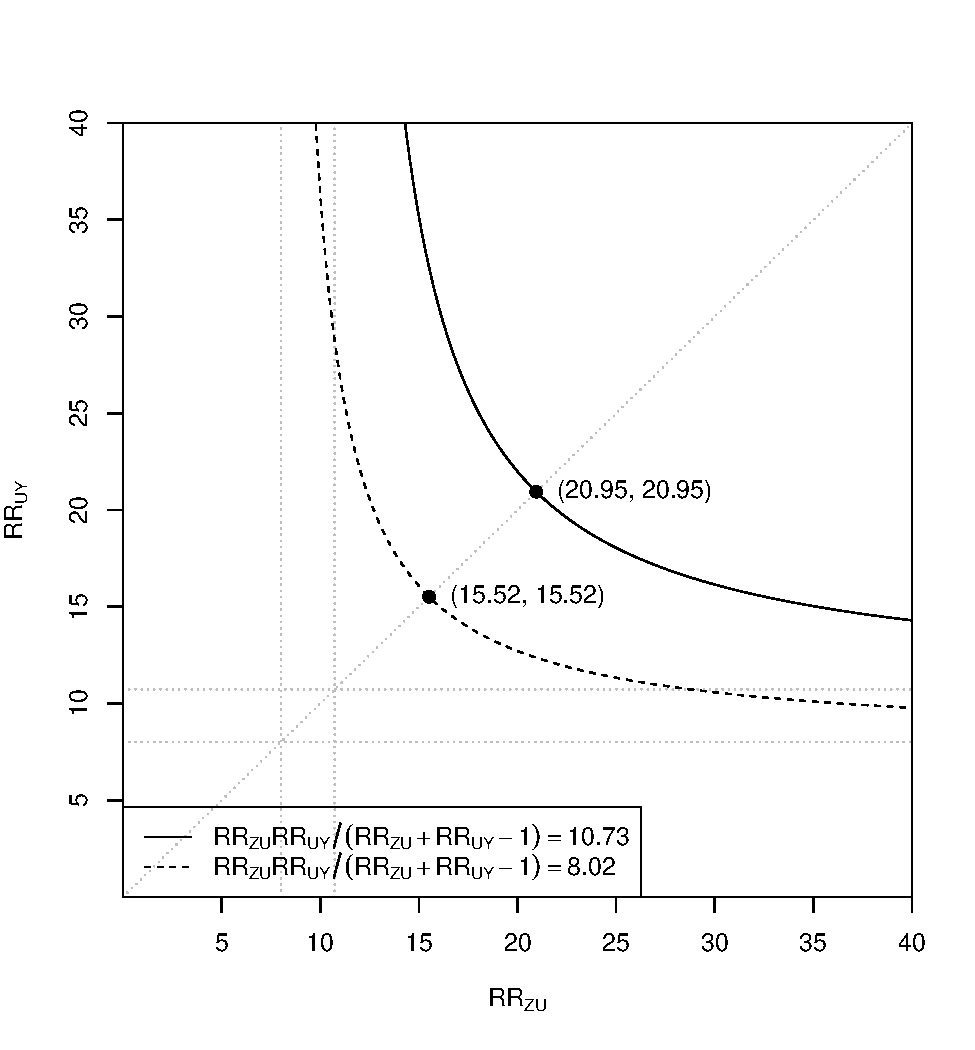
\includegraphics[width = 0.8 \textwidth]{figures/jointvalueplot.pdf}
\caption{完全解释掉\citet{Hammond::1968}数据中的观测风险比所需的混杂强度}\label{fg::hammond-e-value}
\end{figure}



\section{推广}


\subsection{E 值与 Bradford Hill 因果判断标准}

E 值提供支持因果关系的证据，但证据并不等于证明。E 值越大，要解释掉观测风险比所需的未测量混杂就越强，因果证据也越强；E 值越小，较弱的未测量混杂就足以解释观测风险比，因果证据也越弱。结合第\ref{sec::evalue-monotone}节可知，较大的观测风险比提供较强的因果证据。这与 Bradford Hill 爵士提出的第一条因果判断标准密切相关，即关联的{\it 强度}\citep{hill1965environment}。定理\ref{thm::bounding-factor}对这一直观论证给出了数学量化。 


在一篇著名论文中，\citet{hill1965environment}提出了九条标准，用来评价假定原因与结果之间的因果证据。


\begin{definition}\label{def::hill-causation}
Bradford Hill 给出了九条因果判断标准：
\begin{enumerate}
\item
关联强度；
\item
一致性；
\item
特异性；
\item
时间先后关系；
\item
生物学梯度；
\item
合理性；
\item
连贯性；
\item
实验；
\item
类比。
\end{enumerate}
\end{definition}


E 值为第一条标准提供了一种依据：更强的关联往往提供更强的因果证据，因为解释掉更强的关联，需要更强的混杂。第\ref{part::rcts}部分讨论的随机实验呼应了第八条标准。篇幅所限，这里不详述其他标准，建议阅读\citet{hill1965environment}。这篇论文最近以\citet{hill2020environment}重新刊载，并附有多位因果推断学者富有见地的评论。 




\subsection{逻辑回归后的 E 值}

对于二元结果，流行病学研究常将结果$Y_i$对处理指标$Z_i$和协变量$X_i$作逻辑回归：
$$
\pr(Y_i = 1\mid Z_i, X_i) = \frac{  e^{\beta_0 + \beta_1 Z_i + \beta_2\tran X_i}  }{1  + e^{\beta_0 + \beta_1 Z_i + \beta_2\tran X_i}} .
$$
在这一模型中，$Z_i$的系数是在给定协变量后处理与结果之间条件优势比的对数：
$$
\beta_1 = \log \frac{   \pr(Y_i=1\mid Z_i =1, X_i=x)/  \pr(Y_i=0\mid Z_i =1, X_i=x)  }
{  \pr(Y_i=1\mid Z_i =0, X_i=x)/  \pr(Y_i=0\mid Z_i =0, X_i=x)  }  .
$$
模型假定所有协变量取值下的优势比相同。此外，若结果罕见，即$ \pr(Y_i=1\mid Z_i =1, X_i=x)$与$\pr(Y_i=1\mid Z_i =0, X_i=x)$都接近$0$，条件优势比就近似于条件风险比（见命题\ref{prop::2x2-independence}(3)）：
$$
\beta_1  \approx \log  \frac{   \pr(Y_i=1\mid Z_i =1, X_i=x)  }
{  \pr(Y_i=1\mid Z_i =0, X_i=x)  } = \log   \RR_{ZY\mid x}^\obs.
$$
因此，可以直接根据逻辑回归系数的估计及其置信限计算 E 值。这是 E 值最主要的应用。 




\begin{example}
\label{eg::NCHS2003}
\ri{NCHS2003.txt}包含美国国家卫生统计中心的出生证明数据，下列二元指标变量与本例有关：


 

\begin{tabular}{ll}
\hline 
\texttt{PTbirth} &
 早产 \\
\texttt{preeclampsia} &
 子痫前期 \\
\texttt{ageabove35}& 
 年龄$\geq 35$的高龄产妇（处理变量） \\
\texttt{somecollege}&
 大学教育 \\
\texttt{mar}& 
 婚姻状况 \\
\texttt{smoking}& 
 吸烟状况 \\
\texttt{drinking}& 
 饮酒状况 \\
\texttt{hispanic}& 
 母亲的族裔  \\
\texttt{black}& 
 母亲的族裔  \\
\texttt{nativeamerican}& 
 母亲的族裔 \\
\texttt{asian}& 
 母亲的族裔\\
 \hline 
\end{tabular} 



本例使用的数据版本来自\citet{valeri2014estimation}。这里以\ri{PTbirth}为结果，习题\ref{hw::eg::NCHS2003}则以\ri{ pre-eclampsia}为结果；后者是妊娠期一种累及多系统的高血压疾病。下面的\ri{R}代码在拟合逻辑回归后计算 E 值。结果表明，要完全解释掉点估计，最大混杂强度必须大于 1.94；要解释掉置信下限，最大混杂强度必须大于 1.91。这些强度虽不及第\ref{sec::evalue-example}节中的数值，在流行病学研究中仍相当大。 
\end{example}


下面的简单\ri{R}代码计算例\ref{eg::NCHS2003}中的数值： 
 \begin{lstlisting}
> NCHS2003 = read.table("NCHS2003.txt", header = TRUE, sep = "\t")
> ## outcome: PTbirth
> y_logit = glm(PTbirth ~ ageabove35 + 
+                 mar + smoking + drinking + somecollege + 
+                 hispanic + black + nativeamerican + asian,
+               data = NCHS2003, 
+               family = binomial)
> log_or   = summary(y_logit)$coef[2, 1:2]
> est      = exp(log_or[1])
> lower.ci = exp(log_or[1] - 1.96*log_or[2])
> est
Estimate 
1.305982 
> evalue(est)
Estimate 
1.938127 
> lower.ci
Estimate 
1.294619 
> evalue(lower.ci)
Estimate 
1.912211 
\end{lstlisting}


\subsection{真实因果效应不为零}
 
定理\ref{thm::bounding-factor}假定处理对结果没有真实因果效应。\citet{ding2016sensitivity}证明了允许真实因果效应非零的一般定理。


\begin{theorem}
\label{thm::general-evalue}
将$\RR_{UY\mid x}   $重新定义为
$$
 \RR_{UY\mid x}  =  \max_{z=0,1} \frac{  \pr(Y=1\mid Z=z, U=1, X=x) }{  \pr(Y=1\mid Z=z, U=0, X=x) }.
$$
假定\eqref{eq::largerthan1-evalue}，则有
$$
\RR_{ZY\mid x}^\true \geq 
\RR_{ZY\mid x}^\obs \Big /  \frac{ \RR_{ZU\mid x}  \RR_{UY\mid x} }{  \RR_{ZU\mid x} + \RR_{UY\mid x} - 1} .
$$
\end{theorem}

当$\RR_{ZY\mid x}^\true   = 1.$时，定理\ref{thm::bounding-factor}是定理\ref{thm::general-evalue}的特例。定理\ref{thm::general-evalue}的证明见\citet{ding2016sensitivity}的原论文。在不加额外假设的情况下，定理\ref{thm::general-evalue}根据观测风险比$\RR_{ZY\mid x}^\obs$及敏感性参数$\RR_{ZU\mid x} $和$ \RR_{UY\mid x}$，给出了真实风险比$\RR_{ZY\mid x}^\true$的下界。 


当处理表面上对结果具有预防作用时，观测风险比小于 1，不能直接使用定理\ref{thm::bounding-factor}和\ref{thm::general-evalue}。此时必须重新编码处理水平，并根据$1/ \RR_{ZY\mid x}^\obs$计算 E 值。 




\section{批评与回应}

自最初论文发表以来，E 值已成为许多流行病学研究常规报告的数值，但也受到批评\citep{ioannidis2019limitations}。下面回顾它的若干局限。 



\subsection{E 值只是风险比的单调变换}
\label{sec::evalue-monotone}

\begin{figure}
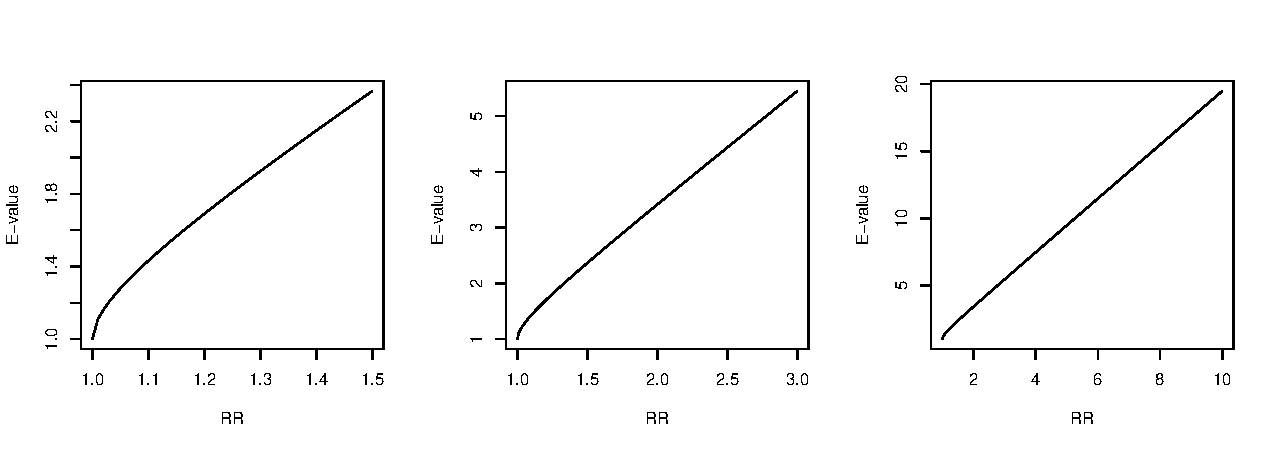
\includegraphics[width=\textwidth]{figures/value_rr.pdf}
\caption{作为风险比单调变换的 E 值：三幅图使用不同的风险比范围}\label{fig::evalue-rr}
\end{figure}

图\ref{fig::evalue-rr}表明，风险比较大时，E 值$\RR_{ZY\mid x}^\obs + \sqrt{ \RR_{ZY\mid x}^\obs (\RR_{ZY\mid x}^\obs - 1)}$接近$2 \RR_{ZY\mid x}^\obs$，几乎与风险比呈线性关系；风险比较小时，它关于$ \RR_{ZY\mid x}^\obs$的非线性更明显。批评者常指出，E 值只是风险比点估计或置信限的单调变换，因此没有提供额外信息。 


这一说法部分成立：E 值确实完全由风险比的点估计或置信限决定。但定理\ref{thm::bounding-factor}赋予它有意义的解释：要完全解释掉观测风险比，两个混杂强度中的最大者必须至少达到 E 值。 







%\subsection{E-value is only one-sided}
%
%
%In classic statistics, the $p$-value is often criticized to be one-sided. That is, we reject the null hypothesis with a small $p$-value, but we often do not say that we accept the null hypothesis with a large $p$-value. 
%A large $p$-value may be due to many other reasons, e.g., the sample size is small, the test statistics lack power, etc.
%The E-value has a similar problem. We are more comfortable saying that the causal evidence is weak with a small E-value, but we may be more conservative in claiming strong causal evidence 
%The critiques in some sense apply to all sensitivity analysis techniques in causal inference. 


\subsection{E 值的校准}



E 值给出一个阈值：要完全解释掉观测关联，混杂变量与处理、混杂变量与结果的两种关联强度中，最大者至少需要达到这一数值。一个明显困难是，混杂变量本身不可观测，因此判断某个 E 值究竟算大还是小并不容易。此外，E 值衡量给定$X$后的残余混杂，因而依赖于已经控制了哪些、多少观测协变量$X$。所以，不同研究的 E 值不能直接比较。E 值提供因果证据，但必须结合具体问题的背景知识谨慎评价。 


一种直观的校准方法是逐次留出一个协变量。令$X = (X_1, \ldots, X_p)$，假装其中的$X_j$未被观测到，在控制其余观测协变量后，分别计算$Z$与$X_j$、$X_j$与$Y$的风险比，$(j=1, \ldots, p)$。若相信未测量变量$U$的混杂作用不强于某些已观测协变量，这些风险比就能为$U$导致的混杂强度提供参照范围。不过，我尚不知道这一方法是否有正式的理论论证。 



\subsection{最适用于二元结果与风险比}


定理\ref{thm::bounding-factor}适合分析二元结果和风险比。\citet{ding2016sensitivity}也提出了其他因果参数的敏感性分析方法，包括二元结果的风险差、非负结果的均值比以及生存结果的风险率比，但它们都不如基于风险比的二元结果 E 值简洁。下一章将提出一种简单的平均因果效应敏感性分析方法，可将第\ref{part::observational-studies}部分的结果回归、IPW 和双重稳健估计量作为特例。 





\section{作业习题}


\paragraph{证明定理\ref{thm::bounding-factor}所需的技术引理}
\label{hw::technical-for-evalue-increasing}

证明函数
$$
f(x) = \frac{ax+1}{bx+1}
$$
在$a>b$时随$x$递增，在$a<b$时随$x$递减。 


\paragraph{定理\ref{thm::bounding-factor}的技术假设}
\label{hw::technical-largerthan1}

重新考察定理\ref{thm::bounding-factor}的证明。假设$Z\ind Y \mid (X, U)$，证明：若$ \RR_{ZU\mid x} > 1$但$ \RR_{UY\mid x} < 1$，则$\RR_{ZY\mid x}^\obs < 1$。 


注：这个结论很直观。在给定$X.$后，如果$Z$与$U$正相关、$U$与$Y$负相关，而且给定$U$后$Z$与$Y$条件独立，那么$Z$与$Y$负相关。由此，若$\RR_{ZY\mid x}^\obs > 1$且$ \RR_{ZU\mid x} > 1$，则$ \RR_{UY\mid x} > 1$必须成立。所以，\eqref{eq::largerthan1-evalue}中的第三个条件实际上是多余的。 



\paragraph{引理\ref{lemma::betaw1w2}}\label{hw::proof-lemma-evalue}

证明引理 \ref{lemma::betaw1w2}。

\paragraph{\citet{Schlesselman::1978}的公式}\label{hw::Schlesselman1978formula}

为简化记号，本题始终隐含以$X$为条件。考虑二元处理$Z$、结果$Y$与未测量混杂变量$U$。假定在$U=0$和$U=1$两层中，处理与结果的风险比相同：
$$
%\RR_{ZY}^{\true}  =
 \RR_{ZY|U=0} = \RR_{ZY|U=1}, 
$$
并假定在$Z=0$和$Z=1$两层中，混杂变量与结果的风险比也相同：
$$  
\RR_{UY|Z=0} = \RR_{UY|Z=1} , \text{ denoted by }\gamma.
$$

证明
$$
\frac{\RR_{ZY}^{\obs}}{  \RR_{ZY}^{\true} } = \frac{1 + (  \gamma  -1)\pr(U=1\mid Z=1)  }
{ 1 + (  \gamma -1)\pr(U=1\mid Z=0) } .
$$ 




注：先验证，若$\RR_{ZY|U=0} = \RR_{ZY|U=1}$，则
$$
\RR_{ZY}^{\true}  = \RR_{ZY|U=0} = \RR_{ZY|U=1} . 
$$
这个恒等式说明了风险比的{\it 可折叠性}。在流行病学中，风险比是一种{\it 可折叠的}关联度量。


 
\citet{Schlesselman::1978}的公式不假定条件独立性$Z\ind Y\mid U$，但假定$Z$与$Y$、$U$与$Y$的风险比分别具有齐性。这是经典的敏感性分析恒等式；预先指定
$$
\{   \gamma  ,  \pr(U=1\mid Z=1), \pr(U=1\mid Z=0)  \} .
$$
即可方便地使用。但它涉及的敏感性参数多于定理\ref{thm::bounding-factor}。虽然定理\ref{thm::bounding-factor}只给出不等式，与依赖更强假设的\citet{Schlesselman::1978}公式相比，这个不等式并不宽松。有了定理\ref{thm::bounding-factor}后，\citet{Schlesselman::1978}公式主要具有历史意义。 



 
\paragraph{逻辑回归后的 E 值：数据分析}\label{hw::eg::NCHS2003}

本题使用与例\ref{eg::NCHS2003}相同的数据集。 

报告以\ri{preeclampsia}为结果时的 E 值。 


\paragraph{风险差的 Cornfield 型不等式}\label{hw::cornfield-rd}



考虑二元变量$Z, Y, U$，隐含以$X$为条件，并假定给定$U$后满足潜在可忽略性。证明在$Z\ind Y\mid U$下，
\begin{eqnarray}
\RD_{ZY}^\obs = \RD_{ZU} \times \RD_{UY}
\label{eq::cornfield-rd}
\end{eqnarray}
其中$\RD_{ZY}^\obs$是$Z$与$Y$的观测风险差，$\RD_{ZU}$和$ \RD_{UY}$分别是处理与混杂变量、混杂变量与结果的风险差（回顾第\ref{sec::twobytwotables-withresume}节的风险差定义）。 


注：不失一般性，假定$\RD_{ZY}^\obs, \RD_{ZU} ,\RD_{UY}$均为正。由\eqref{eq::cornfield-rd}可得
$$
\min(\RD_{ZU}  , \RD_{UY}) \geq \RD_{ZY}^\obs
$$
和
$$
\max(\RD_{ZU}  , \RD_{UY}) \geq  \sqrt{ \RD_{ZY}^\obs} .
$$
这就是二元混杂变量下风险差的 Cornfield 不等式。它们说明，要解释掉观测风险差$\RD_{ZY}^\obs$，处理与混杂变量、混杂变量与结果的两个风险差都不能小于$\RD_{ZY}^\obs$，而两者中的最大值不能小于$\RD_{ZY}^\obs$的平方根。

\citet{Cornfield::1959}已经得到了\eqref{eq::cornfield-rd}，但未充分认识其意义。\citet{gastwirth1998cornfield}和\citet{poole2010origin}讨论了风险差的第一条 Cornfield 条件，\citet{ding2014generalized}讨论了第二条。 

\citet{ding2014generalized}还推导了不要求$U$为二元变量的一般结论。遗憾的是，对于一般$U$，结论弱于二元$U$的情形：$U$的取值水平越多，不等式就越宽松。这促使\citet{ding2016sensitivity}转而研究风险比的 Cornfield 不等式，因为它们不会随着$U$的取值水平增加而变弱。




\paragraph{推荐阅读}


\citet{ding2016sensitivity}推广并统一了 Cornfield 型敏感性分析，为 E 值概念提供了理论基础。   

  
  
\chapter{存在未测混杂因素时平均因果效应的敏感性分析}
\chaptermark{平均因果效应的敏感性分析}\label{chapter::sensitivity-ACE}


 
 
 
 
在给定观测协变量后，Cornfield 型敏感性分析最适合处理以风险比衡量效应的二元结果。尽管\citet{ding2016sensitivity}也提出了针对平均因果效应的 Cornfield 型敏感性分析方法，这些方法仍不够一般，应用起来也不方便。下面基于潜在结果的条件期望介绍一种更直接的方法，其优点是在敏感性分析框架下能够处理常用的平均因果效应估计量。这个思路已见于\citet{robins1999association}和\citet{scharfstein1999adjusting}的早期工作。本章采用\citet{luding2023flexible}近期提出的表述。  
 
 
 
 
 该方法与推导平均潜在结局最坏情况界限的思路密切相关。我将先介绍界限推导这一较为简单的思路，随后将其扩展至敏感性分析领域。 



\section{引言}


回顾典型观测研究场景：观测数据满足 $\{  Z_i, X_i,  Y_i(1), Y_i(0) \}_{i=1}^n \iidsim  \{ Z, X, Y(1), Y(0) \}$，重点关注平均因果效应：
$$
\tau = E\{ Y(1) - Y(0) \}.
$$
该值可分解为：
\begin{eqnarray*}
\tau &=& \left[  E(Y\mid Z=1) \pr(Z=1) + E\{ Y(1)\mid Z=0 \} \pr(Z=0) \right]  \\
&&- \left[   E\{ Y(0)\mid Z=1\} \pr(Z=1) + E(Y\mid Z=0)  \pr(Z=0)  \right] . 
\end{eqnarray*}
因此核心难点在于估计反事实均值：
$$
E\{ Y(1)\mid Z=0 \}  ,\quad \quad E\{ Y(0)\mid Z=1\}.
$$
理论上存在两种极端估计策略。



第一种策略即前文 \ref{part::observational-studies} 所述方法，其成立前提是忽略性假设：
\begin{eqnarray*}
E\{ Y(1)\mid Z=1, X \} &=& E\{ Y(1)\mid Z=0, X \} ,\\ 
E\{ Y(0)\mid Z=1, X \} &=& E\{ Y(0)\mid Z=0, X \}, 
\end{eqnarray*}
在此前提下可通过观测数据确定反事实均值：
$$
E\{ Y(1)\mid Z=0 \}  
%= E\left[ E\{ Y(1)\mid Z=0, X \}  \mid Z=0 \right] 
%= E\left[ E\{ Y(1)\mid Z=1, X \}  \mid Z=0\right] 
= E\left\{  E( Y\mid Z=1, X )  \mid Z=0\right\}
$$
同理：
$$
E\{ Y(0)\mid Z=1\} = E\left\{  E( Y\mid Z=0, X )  \mid Z=1\right\} . 
$$



下一节介绍的第二种策略只假定结果位于$\underline{y}$与$\overline{y}$之间。对于取$\underline{y} = 0$和$\overline{y} = 1$的二元结果，这个假设自然成立。此时两个反事实均值也位于$\underline{y}$与$\overline{y}$之间，从而得到$\tau$的最坏情形界。表\ref{table::manski-bounds}说明了基本思路，第\ref{sec::manski-bounds}节将作更详细的回顾。 


 


 



\begin{table}
\centering
\caption{结局值受限 $ [\underline{y}, \overline{y}]$ 时的分析表格，$\underline{y}$ 与 $\overline{y}$ 为给定常数}\label{table::manski-bounds}
\begin{tabular}{ccccccc}
\hline 
$Z$ & $Y(1)$ & $Y(0)$ &  $Y(1)$ 下限 & $Y(1)$ 上限 & $Y(0)$ 下限 & $Y(0)$ 上限 \\
\hline 
$1$ & $Y_1(1)$ & ? & $Y_1(1)$  & $Y_1(1)$ & $\underline{y}$ & $\overline{y}$ \\
$\vdots$&$\vdots$&$\vdots$&$\vdots$&$\vdots$&$\vdots$&$\vdots$   \\
$1$ & $Y_{n_1}(1)$ & ? &  $Y_{n_1}(1)$  & $Y_{n_1}(1)$ & $\underline{y}$ & $\overline{y}$ \\
\hline 
$0$ & ? & $Y_{n_1+1}(0)$ & $\underline{y}$ & $\overline{y}$& $Y_{n_1+1}(0)$ & $Y_{n_1+1}(0)$ \\ 
$\vdots$&$\vdots$&$\vdots$&$\vdots$&$\vdots$&$\vdots$&$\vdots$ \\ 
$0$ & ? & $Y_{n}(0)$ & $\underline{y}$ & $\overline{y}$& $Y_{n}(0)$ & $Y_{n}(0)$ \\
\hline 
\end{tabular}
\end{table}


\section{无需额外假设的Manski型平均因果效应最坏情况界限}\label{subsection::manski-bounds}
\label{sec::manski-bounds}



假设结果有界，取值介于$\underline{y}$与$\overline{y}$之间。根据分解
$$
E\{  Y(1) \} = E\{  Y(1) \mid Z=1\} \pr(Z=1)  +  E\{  Y(1) \mid Z=0\} \pr(Z=0)  ,
$$
可得$E\{  Y(1) \}$的下界
$$
E\{  Y \mid Z=1\} \pr(Z=1)  +   \underline{y} \pr(Z=0) 
$$
和上界
$$
E\{  Y \mid Z=1\} \pr(Z=1)  +  \overline{y} \pr(Z=0).
$$
类似地，根据分解
$$
E\{  Y(0) \} = E\{  Y(0) \mid Z=1\} \pr(Z=1)  +  E\{  Y(0) \mid Z=0\} \pr(Z=0)  ,
$$
可得$E\{  Y(0) \}$的下界
$$
\underline{y}\pr(Z=1)  +  E\{  Y \mid Z=0\} \pr(Z=0) 
$$
和上界
$$
 \overline{y} \pr(Z=1)  +  E\{  Y \mid Z=0\} \pr(Z=0). 
$$
结合这些界，可得平均因果效应$\tau = E\{  Y(1) \} - E\{  Y(0) \}$的下界
$$
E\{  Y \mid Z=1\} \pr(Z=1)  +   \underline{y} \pr(Z=0) - \overline{y} \pr(Z=1)  -  E\{  Y \mid Z=0\} \pr(Z=0) 
$$
和上界
$$
 E\{  Y \mid Z=1\} \pr(Z=1)  +  \overline{y} \pr(Z=0) - \underline{y}\pr(Z=1)  -   E\{  Y \mid Z=0\} \pr(Z=0). 
$$
该区间的长度为$\overline{y}-\underline{y}$。这些界提供的信息有限，但仍优于长度为$2(\overline{y}-\underline{y})$的先验界$[\underline{y}-\overline{y}, \overline{y}-\underline{y}]$。若不作进一步假设，观测数据的分布无法唯一确定$\tau$。此时称$\tau$是{\it 部分识别的}，其正式定义如下。 


\begin{definition}
[部分可识别]\label{def::partial-identification}
若观测数据分布可对应多个 $\theta$ 取值，则称参数 $\theta$ 为部分可识别。 
\end{definition}


对比定义 \ref{def::nonparametric-identification} 与 \ref{def::partial-identification}。若参数 $\theta$ 能由观测数据唯一确定则为可识别，否则仅为部分可识别。故在忽略性假设成立时 $\tau$ 可识别，否则仅为部分可识别。 




\citet{cochran1953}曾在存在缺失数据的调查中使用最坏情形界，但由于结果往往过于保守而放弃了这一思路。同样，上述$\tau$的最坏情形界通常包含$0$，因而在实践中往往意义不大。此外，这种策略不适用于结果无界的情形。 



Manski将此思路成功应用于因果推断 \citep{manski1990nonparametric} 及多种计量经济模型 \citep{manski2003partial}。在辅以其他定性假设的前提下，这种基于最小假设的界限推导法极具实用价值。\citet{manski2003partial} 系统梳理了多种适用策略。例如可引入单调性假设：
$
Y(1)\geq Y(0) . 
$
此时 $\tau$ 下界降为零而上界不变。亦可设定：
$Z = I\{  Y(1) \geq Y(0) \}$，即治疗选择基于潜在结局差值。此类假设均能优化 $\tau$ 的界限估计。更多细节探讨已超出本书范围。 

 
 


 
\section{平均因果效应的敏感性分析}


 
第一种策略持乐观态度，假设给定观测协变量时处理组与对照组的潜在结局无差异。第二种策略则较悲观，完全不依赖观测数据推断反事实均值。下文介绍的方法介于二者之间。 



\subsection{识别公式推导}

定义：
\begin{eqnarray*}
\frac{ E\{ Y(1)\mid Z=1, X \} }{ E\{ Y(1)\mid Z=0, X \} } = \varepsilon_1(X), \\
\frac{ E\{ Y(0)\mid Z=1, X \} }{ E\{ Y(0)\mid Z=0, X \} } = \varepsilon_0(X) ,
\end{eqnarray*}
上述参数即敏感性参数。为简化分析可假定二者与 $X$ 无关。实际应用时需预先设定其取值范围。令 $\mu_1(X) = E(Y\mid Z=1, X)$ 与 $\mu_0(X) = E(Y\mid Z=0, X)$ 分别为处理组与对照组的条件均值函数。此时可推导出： 

\begin{theorem}
\label{thm::outcome-reg-sensitivity}
已知$\varepsilon_1(X)$和$ \varepsilon_0(X) $时，有
\begin{eqnarray*}
E\{ Y(1)\mid Z=0 \}   &=& E\left\{\mu_1(X)   / \varepsilon_1(X)  \mid Z=0\right\},\\ 
E\{ Y(0)\mid Z=1 \}   &=& E\left\{\mu_0(X)    \varepsilon_0(X)  \mid Z=1\right\}
\end{eqnarray*}
因而
\begin{eqnarray}
\tau & = & E\{ ZY + (1-Z) \mu_1(X)   / \varepsilon_1(X)\}  \nonumber  \\
 && - E\{ Z \mu_0(X)    \varepsilon_0(X) + (1-Z)Y\}  \label{eq::predictive}\\
& = & E\{ Z \mu_1(X) + (1-Z) \mu_1(X)   / \varepsilon_1(X)\}  \nonumber \\
&&- E\{ Z \mu_0(X)    \varepsilon_0(X) + (1-Z) \mu_0(X)\}. \label{eq::projective}
\end{eqnarray}
\end{theorem}


 


定理\ref{thm::outcome-reg-sensitivity}的证明留作习题\ref{hw::proof-theorem-1-sa}。根据拟合的结果模型，\eqref{eq::predictive}和\eqref{eq::projective}给出$\tau$的如下预测型和投影型估计量：
\begin{eqnarray*}
\hat\tau^{\textup{pred}} &=&\left\{  n^{-1}\sumn Z_i Y_i + n^{-1} \sumn (1-Z_i) \hat{\mu}_1(X_i)   / \varepsilon_1(X_i)  \right\} \\
&&- \left\{ n^{-1}  \sumn Z_i \hat{\mu}_0(X_i)    \varepsilon_0(X_i) + n^{-1} \sumn (1-Z_i) Y_i \right\},
\end{eqnarray*}
以及
\begin{eqnarray*}
\hat{\tau}^{\textup{proj}}&=&\left\{ n^{-1}\sumn Z_{i}\hat{\mu}_{1}(X_{i})+n^{-1}\sumn(1-Z_{i})\hat{\mu}_{1}(X_{i})/\varepsilon_{1}(X_{i})\right\} \\
&&-\left\{ n^{-1}\sumn Z_{i}\hat{\mu}_{0}(X_{i})\varepsilon_{0}(X_{i})+n^{-1}\sumn(1-Z_{i})\hat{\mu}_{0}(X_{i})\right\}.
\end{eqnarray*}
“预测型”和“投影型”的名称来自抽样调查文献\citep{firth1998robust, ding2018causal}；另见第\ref{sec::understand-lin-predict}章。估计量$\hat\tau^{\textup{pred}} $与$\hat{\tau}^{\textup{proj}}$略有不同：前者在观测结果可用时使用观测值，后者则用拟合值替代观测结果。 





更有价值的是基于逆概率加权法推导 $\tau$ 估计量：

\begin{theorem}\label{thm::ipw-sensitivity}
已知 $\varepsilon_1(X)$ 与 $ \varepsilon_0(X) $ 时，有
\begin{eqnarray*} 
E\{ Y(1) \} = 
E\left\{ w_1(X) \frac{Z}{e(X)}  Y  \right\}  ,\quad
 E\{Y(0)\} = E\left\{ w_0(X) \frac{1-Z}{1-e(X)} Y \right\},
\end{eqnarray*}
此处
$$
w_1(X) = e(X) + \{1-e(X)\}/ \varepsilon_1(X) ,\quad
w_0(X) = e(X)  \varepsilon_0(X) + 1- e(X). 
$$
\end{theorem}


 
 

定理\ref{thm::ipw-sensitivity}的证明留作习题\ref{hw::proof-theorem-2-sa}。定理\ref{thm::ipw-sensitivity}在经典 IPW 公式中加入了$w_1(X) $和$w_0(X) $两个因子，它们均依赖于倾向得分和敏感性参数。利用拟合的倾向得分，定理\ref{thm::ipw-sensitivity}给出$\tau$的如下估计量：
\begin{eqnarray*} 
\hat\tau^{\textup{ht}} &=&  n^{-1} \sumn \frac{ \{ \hat{e}(X_i)\varepsilon_1(X_i) + 1-\hat{e}(X_i) \} Z_iY_i     }{  \varepsilon_1(X_i)  \hat e(X_i)  } \\
&&- n^{-1} \sumn  \frac{ \{  \hat e(X_i)  \varepsilon_0(X_i) + 1- \hat e(X_i)  \} (1-Z_i) Y_i }{ 1- \hat e(X_i)} 
\end{eqnarray*}
以及
\begin{eqnarray*} 
\hat\tau^{\textup{haj}} &=&   \sumn \frac{ \{ \hat{e}(X_i)\varepsilon_1(X_i) + 1-\hat{e}(X_i) \} Z_iY_i     }{  \varepsilon_1(X_i)  \hat  e(X_i)  }  \Big / \sumn \frac{Z_i}{ \hat{e}(X_i)  }   \\
&&- n^{-1} \sumn  \frac{ \{  \hat  e(X_i)  \varepsilon_0(X_i) + 1- \hat e(X_i)  \} (1-Z_i) Y_i }{ 1- \hat e(X_i)} \Big / \sumn \frac{1-Z_i}{ 1- \hat{e}(X_i)  } .
\end{eqnarray*}





更有意思的是，利用拟合的倾向得分和结果模型，下列$\tau$的估计量具有双重稳健性：
\begin{eqnarray*}
\hat{\tau}^{\textup{ht}} = \hat\tau^{\textup{ht}} 
- n^{-1} \sumn \{Z_i- \hat e(X_i)\}  \left\{   \frac{  \hat  \mu_1(X_i) }{  \hat e(X_i) \varepsilon_1(X_i)  }    + \frac{  \hat  \mu_0(X_i)\varepsilon_0(X_i)  }{ 1-  \hat  e(X_i) } \right\}.
\end{eqnarray*}
也就是说，在$\varepsilon_1(X_i) $和$\varepsilon_0(X_i) $已知时，只要倾向得分模型或结果模型中至少一个设定正确，$\hat{\tau}^{\textup{dr}} $就是$\tau$的一致估计量。上述估计量的方差可用自助法近似，技术细节参见\citet{luding2023flexible}。 




当 $\varepsilon_1(X_i)  =  \varepsilon_0(X_i) = 1$ 时上述估计量分别退化为前文 \ref{part::observational-studies} 所述预测型、IPW型及双重稳健估计法。 



\subsection{实例演示}
\label{sec::eg-sensitivity-tau}


\subsubsection{敏感性分析的R语言实现}


下面的\ri{R}函数计算敏感性分析所需的点估计。 

\begin{lstlisting}
OS_est_sa = function(z, y, x, out.family = gaussian, 
                     truncps = c(0, 1), e1 = 1, e0 = 1)
{
     ## fitted propensity score
     pscore   = glm(z ~ x, family = binomial)$fitted.values
     pscore   = pmax(truncps[1], pmin(truncps[2], pscore))
     
     ## fitted potential outcomes
     outcome1 = glm(y ~ x, weights = z, 
                    family = out.family)$fitted.values
     outcome0 = glm(y ~ x, weights = (1 - z), 
                    family = out.family)$fitted.values
     
     ## outcome regression estimator
     ace.reg  = mean(z*y) + mean((1-z)*outcome1/e1) - 
                   mean(z*outcome0*e0) - mean((1-z)*y) 
     ## IPW estimators
     w1 = pscore + (1-pscore)/e1
     w0 = pscore*e0 + (1-pscore)
     ace.ipw0 = mean(z*y*w1/pscore) - 
                   mean((1 - z)*y*w0/(1 - pscore))
     ace.ipw  = mean(z*y*w1/pscore)/mean(z/pscore) - 
                   mean((1 - z)*y*w0/(1 - pscore))/mean((1 - z)/(1 - pscore))
     ## doubly robust estimator
     aug = outcome1/pscore/e1 + outcome0*e0/(1-pscore)
     ace.dr   = ace.ipw0 + mean((z-pscore)*aug)

     return(c(ace.reg, ace.ipw0, ace.ipw, ace.dr))     
}
\end{lstlisting}

标准误计算方式则留作习题 \ref{hw::sensitivity-se} 探讨。 

\subsubsection{重访实例 \ref{eg::chan-bmi-ATE}}


令
$$
\varepsilon_1(X) = \varepsilon_0(X) \in \{1/2, 1/1.7, 1/1.5, 1/1.3, 1, 1.3, 1.5, 1.7, 2\},
$$
用下面的\ri{R}代码可得到一组$\tau$的双重稳健估计：
\begin{lstlisting}
> nhanes_bmi = read.csv("nhanes_bmi.csv")[, -1]
> z = nhanes_bmi$School_meal
> y = nhanes_bmi$BMI
> x = as.matrix(nhanes_bmi[, -c(1, 2)])
> x = scale(x)
> 
> 
> E1 = c(1/2, 1/1.7, 1/1.5, 1/1.3, 1, 1.3, 1.5, 1.7, 2)
> E0 = c(1/2, 1/1.7, 1/1.5, 1/1.3, 1, 1.3, 1.5, 1.7, 2)
> EST = outer(E1, E0)
> ll1 = length(E1)
> ll0 = length(E0)
> for(i in 1:ll1)
+   for(j in 1:ll0)
+     EST[i, j] = OS_est_sa(z, y, x, e1 = E1[i], e0 = E0[j])[4]
\end{lstlisting}




\begin{table}[ht]
\centering
\caption{平均因果效应的敏感性分析结果}\label{table::sensitivity-ACE}
\begin{tabular}{rrrrrrrrrr}
  \hline
 & 1/2 & 1/1.7 & 1/1.5 & 1/1.3 & 1 & 1.3 & 1.5 & 1.7 & 2 \\ 
  \hline
1/2 & 11.62 & 10.44 & 9.40 & 8.03 & 4.96 & 0.97 & -1.69 & -4.35 & -8.34 \\ 
  1/1.7 & 9.22 & 8.05 & 7.00 & 5.64 & 2.57 & -1.42 & -4.08 & -6.75 & -10.74 \\ 
  1/1.5 & 7.63 & 6.45 & 5.41 & 4.05 & 0.97 & -3.02 & -5.68 & -8.34 & -12.33 \\ 
  1/1.3 & 6.03 & 4.86 & 3.81 & 2.45 & -0.62 & -4.61 & -7.27 & -9.94 & -13.93 \\ 
  1 & 3.64 & 2.47 & 1.42 & 0.06 & -3.01 & -7.01 & -9.67 & -12.33 & -16.32 \\ 
  1.3 & 1.80 & 0.63 & -0.42 & -1.78 & -4.85 & -8.85 & -11.51 & -14.17 & -18.16 \\ 
  1.5 & 0.98 & -0.19 & -1.24 & -2.60 & -5.67 & -9.66 & -12.33 & -14.99 & -18.98 \\ 
  1.7 & 0.36 & -0.82 & -1.86 & -3.23 & -6.30 & -10.29 & -12.95 & -15.61 & -19.60 \\ 
  2 & -0.35 & -1.52 & -2.57 & -3.93 & -7.00 & -10.99 & -13.65 & -16.32 & -20.31 \\ 
   \hline
\end{tabular}
\end{table}


表 \ref{table::sensitivity-ACE} 列出了各敏感性参数组合下的估计值。当敏感性参数大于1时估计值符号趋于稳定，小于1时则变化剧烈。若参与计划者BMI值偏高（即 $\varepsilon_1(X) >1$ 且 $ \varepsilon_0(X)  > 1$），则计划对BMI具有负向影响。反之若参与群体BMI偏低，此结论则需谨慎对待。 



\section{作业习题}


\paragraph{定理 \ref{thm::outcome-reg-sensitivity} 证明}\label{hw::proof-theorem-1-sa}

请证明定理 \ref{thm::outcome-reg-sensitivity}。 

\paragraph{定理 \ref{thm::ipw-sensitivity} 证明}\label{hw::proof-theorem-2-sa}

请证明定理 \ref{thm::ipw-sensitivity}。 


\paragraph{敏感性分析的标准误计算}\label{hw::sensitivity-se}

\ref{sec::eg-sensitivity-tau} 章节仅给出点估计值，请补充计算相应的自助法标准误。 

  


\paragraph{处理组平均因果效应$\tau_\textsc{T}$的敏感性分析}\label{hw::att-sentivity-analysis}

本题推广第\ref{chapter::ATT-and-other}章，在允许存在未测量混杂的条件下估计
$$
\tau_\textsc{T} = E\{  Y(1) - Y(0)  \mid Z=1  \} 
= E(Y\mid Z=1) - E\{  Y(0)  \mid Z=1  \} .
$$
$E(Y\mid Z=1)$可以直接用样本矩$\hat{\mu}_{\textsc{t}1} =   \sumn Z_i Y_i / \sumn Z_i$估计。唯一的反事实项是$E\{  Y(0)  \mid Z=1  \}$，因此只需引入敏感性参数$ \varepsilon_0(X) $。当$\varepsilon_0(X) .$已知时，有以下两个识别公式：

\begin{theorem}
\label{thm::att-reg-ipw}
已知$\varepsilon_0(X) $时，
\begin{eqnarray*}
E\{  Y(0)  \mid Z=1  \}  &=& E\left\{  Z \mu_0(X)  \varepsilon_0(X)    \right\} /e \\
&=& E\left\{  e(X)\varepsilon_0(X) \frac{ 1-Z}{1-e(X)}  Y      \right\} /e,
\end{eqnarray*}
其中$e = \pr(Z=1)$。
\end{theorem}


证明定理\ref{thm::att-reg-ipw}。 

注：由定理\ref{thm::att-reg-ipw}，可用$\hat{\tau}_{\textsc{t}}^* = \hat{\mu}_{\textsc{t}1}  - \hat{\mu}_{\textsc{t}0}^*$估计$\tau_{\textsc{t}}$，其中
\begin{eqnarray*}
\hat{\mu}_{\textsc{t}0}^\text{reg} &=& n_1^{-1} \sumn Z_i  \varepsilon_0(X_i) \hat  \mu_0(X_i) ,   \\
\hat{\mu}_{\textsc{t}0}^\text{ht} &=& n_1^{-1} \sumn   \varepsilon_0(X_i) \hat  o(X_i) (1-Z_i) Y_i ,   \\
\hat{\mu}_{\textsc{t}0}^\text{haj} &=&  \sumn   \varepsilon_0(X_i) \hat  o(X_i) (1-Z_i) Y_i  /  \sumn   \hat  o(X_i) (1-Z_i) , 
\end{eqnarray*}
$  \hat  o(X_i) = \hat  e(X_i) / \{1- \hat  e(X_i)\}$是在给定观测协变量后估计的处理条件优势。此外，可以构造$\tau_{\textsc{t}}$的双重稳健估计量$\hat{\tau}_{\textsc{t}}^\text{dr} = \hat{\mu}_{\textsc{t}1}  - \hat{\mu}_{\textsc{t}0}^\text{dr}$，其中
$$
\hat{\mu}_{\textsc{t}0}^\text{dr} = 
\hat{\mu}_{\textsc{t}0}^\text{ht}  - n_1^{-1} \sumn \varepsilon_0(X_i) \frac{\hat e(X_i) - Z}{1-\hat e(X_i)}  \hat \mu_0(X_i)  . 
$$
更详细的讨论参见\citet{luding2023flexible}。 



\paragraph{R语言实现}

实现习题\ref{hw::att-sentivity-analysis}中的估计量，并分析第\ref{sec::eg-sensitivity-tau}节使用的数据。 


\paragraph{推荐阅读}

 \citet{Rosenbaum::1983JRSSB} 与 \citet{imbens2003sensitivity} 为敏感性分析领域的奠基性文献，但所用方法相对复杂，建议读者在掌握基础概念后再行参阅。 


  
    
\chapter{针对存在未观测混杂因素的配对观察性研究的Rosenbaum式$p$值}
\chaptermark{配对研究中的敏感性分析}\label{sec::rosenbaum-sensitivity-analysis}


\citet{rosenbaum1987sensitivity}提出了一种适用于配对观察性研究的敏感性分析技术。虽然该方法也适用于一般的配对研究\citep{rosenbaum2002design}，但在一对一配对的情况下其理论最为完善。与\ref{chapter::evalue}章及\ref{chapter::sensitivity-ACE}章不同，Rosenbaum式敏感性分析最适用于检验“不存在个体治疗效果”这一明确零假设的配对观察性研究。  


\section{基于配对数据的敏感性分析模型}


考虑一项配对观察性研究，用$(i,j)$表示第$i$对中的第$j$个单位$(i=1,\ldots, n; j=1,2)$。精确匹配时，单位$(i, 1)$与单位$(i, 2)$具有相同的协变量$X_i$。假设抽样独立同分布，并推广定义\ref{def::pscore}，将倾向得分定义为
$$
e_{ij} = \pr\{  Z_{ij} = 1\mid X_i, Y_{ij}(1), Y_{ij}(0) \} .
$$
令$\mathbb{S}_i = \{Y_{i1}(1), Y_{i1}(0), Y_{i2}(1), Y_{i2}(0)\}$表示第$i$对中全部潜在结果的集合。在给定事件$Z_{i1} + Z_{i2} = 1$后，
\begin{eqnarray*}
\pi_{i1} &=& \pr\{ Z_{i1} = 1 \mid X_i, \mathbb{S}_i, Z_{i1} + Z_{i2} = 1 \} \\
&=& \frac{ \pr\{ Z_{i1} = 1, Z_{i2} = 0  \mid X_i, \mathbb{S}_i \} }
{ \pr\{ Z_{i1} + Z_{i2} = 1 \mid X_i, \mathbb{S}_i \} } \\
&=& \frac{ \pr\{ Z_{i1} = 1, Z_{i2} = 0  \mid X_i, \mathbb{S}_i \} }{ 
\pr\{ Z_{i1} = 1, Z_{i2} = 0 \mid X_i, \mathbb{S}_i \} + \pr\{ Z_{i1} = 0, Z_{i2} = 1 \mid X_i, \mathbb{S}_i \}
}\\
%{ \left[ \splitfrac{ \pr\{ Z_{i1} = 1, Z_{i2} = 0 \mid X_i, \mathbb{S}_i \} }
%{+\pr\{ Z_{i1} = 0, Z_{i2} = 1 \mid X_i, \mathbb{S}_i \} } \right] } \\
&=& \frac{  e_{i1} (1-e_{i2}) }{ e_{i1} (1-e_{i2}) + (1-e_{i1}) e_{i2}} 
\end{eqnarray*}
定义$o_{ij} = e_{ij} / (1 - e_{ij})$为单位$(i,j)$接受处理的优势，则
$$
\pi_{i1}  = \frac{o_{i1}}{  o_{i1} + o_{i2} } . 
$$
在可忽略性下，$e_{ij}$仅为$X_i$的函数，因此$e_{i1} = e_{i2}$且$\pi_{i1} = 1/2 $。于是，在给定协变量和潜在结果后，处理分配机制等价于处理与对照概率相等的配对实验。这就是第\ref{sec::ideal-matching-mpe}章讨论的分析配对观察性研究的一种策略。 


一般而言，$e_{ij}$还受未观测潜在结果影响，其值可在$0$到$1$之间变化。\citet{rosenbaum1987sensitivity}提出的敏感性分析模型对比值$o_{i1}/o_{i2} $设定了上下限。 

\begin{assumption}[Rosenbaum敏感性分析模型]\label{assume::rosenbaum-sensitivity}
优势比满足以下约束条件：
$$
o_{i1}/o_{i2} \leq \Gamma,\quad
o_{i2}/o_{i1} \leq \Gamma, \quad (i=1, \ldots, n)
$$
其中$\Gamma \geq  1$为预先给定的常数。等价地，
$$ 
\frac{1}{1+\Gamma } \leq 
\pi_{i1} \leq \frac{\Gamma}{1+\Gamma} \quad (i=1, \ldots, n)
$$
同样由$\Gamma \geq  1$决定。
\end{assumption}


在假设\ref{assume::rosenbaum-sensitivity}下，我们得到处理组与对照组概率不均等且随配对变化的偏倚MPE模型。当$\Gamma = 1$时，$\pi_{i1} = 1/2 $，即恢复为标准MPE模型。因此$\Gamma > 1$的数值大小反映了因匹配过程中遗漏变量而导致的对理想MPE模型的偏离程度。 
 
 
 
 \section{Rosenbaum敏感性分析模型下的最坏情况$p$值}


考虑基于对内差
$
\hat{\tau}_i = (2Z_{i1} - 1) (Y_{i1} - Y_{i2}) \  (i=1,\ldots, n). 
$
检验尖锐零假设
$$
\HF: Y_{ij}(1) = Y_{ij}(0) \text{ for } i = 1,\ldots, n \text{ and } j=1,2
$$
在$\HF$下，$|\hat{\tau}_i|$固定，但若$\hat{\tau}_i \neq 0$成立，$S_i = I(\hat{\tau}_i > 0)$仍是随机的。考虑以下一类检验统计量：
$$
T = \sumn S_i q_i,
$$
其中$q_i\geq 0$是$ (|\hat{\tau}_1|, \ldots, |\hat{\tau}_n|   ).$的函数。其特例包括符号统计量、配对$t$统计量（相差一个常数平移）以及 Wilcoxon 符号秩统计量：
$$
T = \sumn S_i,\quad T = \sumn S_i |\hat{\tau}_i|,\quad T = \sumn S_i R_i,
$$
其中$(R_1,\ldots, R_n)$是$ (|\hat{\tau}_1|, \ldots, |\hat{\tau}_n|   ).$的秩。 

对于一般的$\Gamma$，在假设\ref{assume::rosenbaum-sensitivity}下检验统计量$T$的零分布是什么？由于假设\ref{assume::rosenbaum-sensitivity}没有完全规定各$\pi_{i1}$的确切取值，答案可能很复杂。幸运的是，我们不需要知道$T$的确切分布，只需要知道在假设\ref{assume::rosenbaum-sensitivity}下使$p$值最大的$T$的最坏情形分布。该分布对应于
$$
S_i \iidsim  \text{Bernoulli}\left(  \frac{ \Gamma}{ 1+\Gamma} \right).
$$
此时$T$的均值为
$$
E_\Gamma( T ) = \frac{\Gamma}{1+\Gamma} \sumn q_i, 
$$
方差为
$$
\var_\Gamma( T ) = \frac{\Gamma}{(1+\Gamma)^2} \sumn q_i^2,
$$
并具有如下正态分布近似：
$$
\frac{T -\frac{\Gamma}{1+\Gamma} \sumn q_i }{ \sqrt{ \frac{\Gamma}{(1+\Gamma)^2} \sumn q_i^2  }} \rightarrow  \N01 
$$
这里的收敛为依分布收敛。在实践中，可以将一系列$p$值报告为$\Gamma$的函数。 


\section{实例演示}

\subsection{再探LaLonde数据集}\label{sec::rosenbaum-gamma-examples}

 

我们在配对后的LaLonde数据集上实施Rosenbaum式敏感性分析。利用\ri{Matching}包可构建配对数据集： 
\begin{lstlisting}
library("Matching")
library("sensitivitymv")
library("sensitivitymw")
dat <- read.table("cps1re74.csv",header=T)
dat$u74 <- as.numeric(dat$re74==0)
dat$u75 <- as.numeric(dat$re75==0)
y = dat$re78
z = dat$treat
x = as.matrix(dat[, c("age", "educ", "black",
                      "hispan", "married", "nodegree",
                      "re74", "re75", "u74", "u75")])
matchest = Match(Y = y, Tr = z, X = x)
ytreated = y[matchest$index.treated]
ycontrol = y[matchest$index.control]
datamatched = cbind(ytreated, ycontrol)
\end{lstlisting}

考虑使用检验统计量$T = \sumn S_i | \hat{\tau}_i |$。理想配对实验满足$\Gamma = 1$，此时可模拟$T$的分布，得到$p$值$0.002$，见图\ref{fg::lalonde_gamma}的第一个子图。将$\Gamma = 1.1$略微增大后，$T$的最坏情形分布向右移动，$p$值增至$0.011$。若进一步将$\Gamma$增至$1.3$，$T$的最坏情形分布将继续移动，$p$值超过$0.05$。图\ref{fg::p-gamma-lalonde}给出了各$\hat{\tau}_i$的直方图及$p$值随$\Gamma$变化的曲线；$\Gamma  = 1.233$衡量了在$0.05$水平上仍能拒绝零假设时所容许的最大混杂程度。 

也可用\ri{sensitivitymw}包中的\ri{senmw}函数，求出一系列随$\Gamma$变化的$p$值。
\begin{lstlisting}
Gamma  = seq(1, 1.4, 0.001)
Pvalue = Gamma
for(i in 1:length(Gamma))
{
  Pvalue[i] = senmw(datamatched, gamma = Gamma[i], 
                    method = "t")$pval
}
\end{lstlisting}
图\ref{fg::p-gamma-lalonde}给出了$p$值随$\Gamma$变化的曲线。 

 
 
 
 



\begin{figure}
\centering
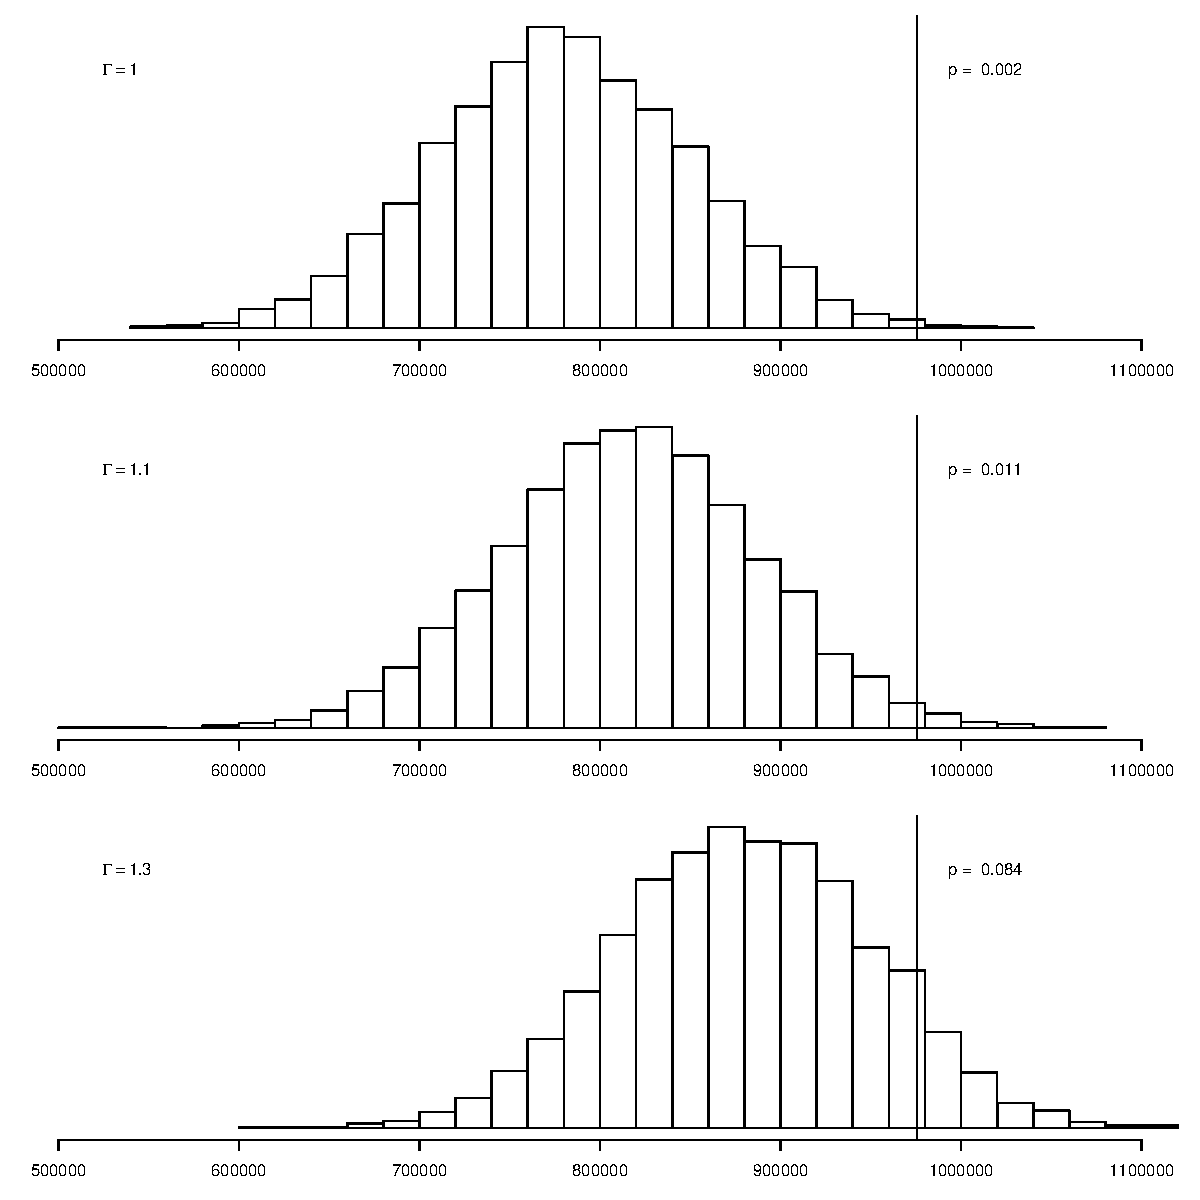
\includegraphics[width =  \textwidth]{figures/lalonde_hist_gamma.pdf}
\caption{基于配对LaLonde数据，满足$S_i$服从独立同分布Bernoulli$(\Gamma/(1+\Gamma))$时$T = \sumn S_i | \hat{\tau}_i |$的最坏情况分布。}\label{fg::lalonde_gamma}
\end{figure} 
 
 
 
 \begin{figure}
\centering
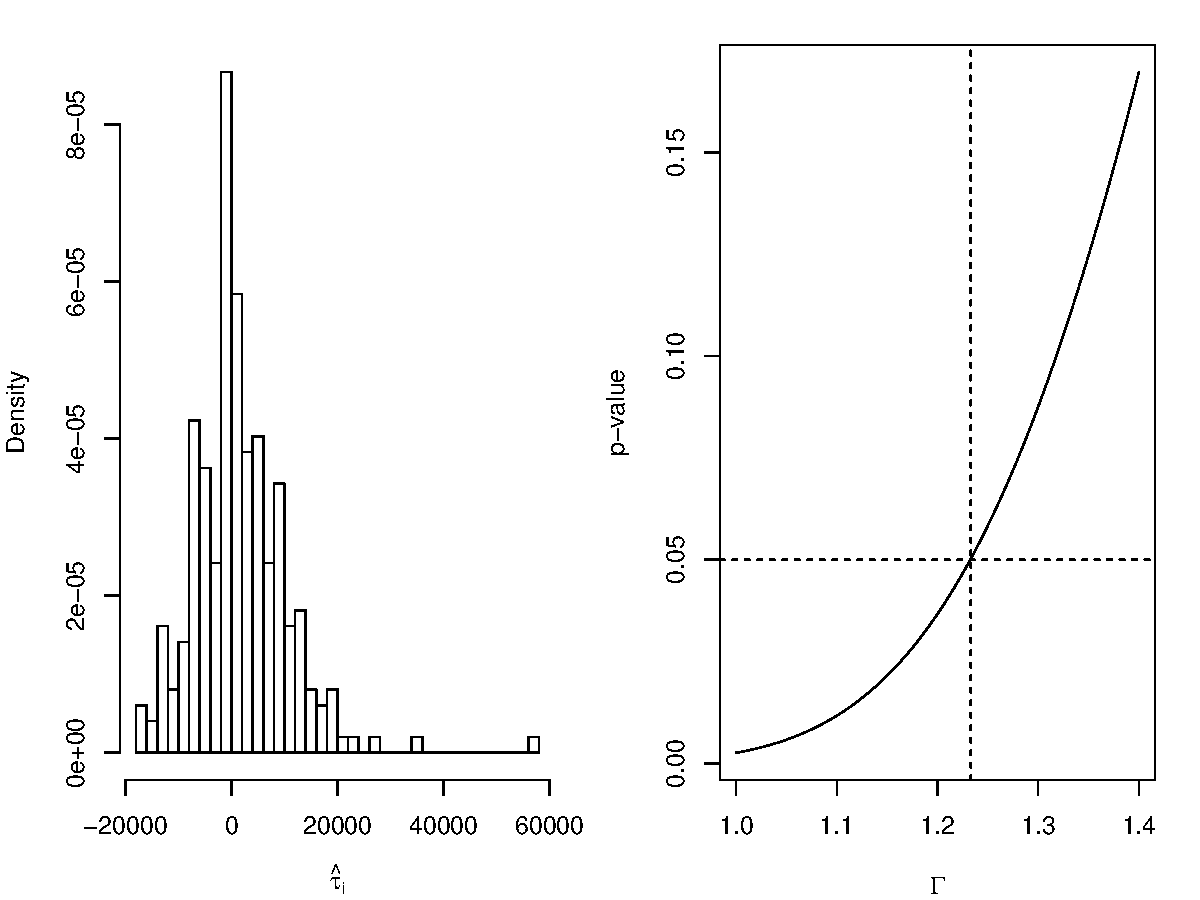
\includegraphics[width = \textwidth]{figures/lalonde_p_gamma.pdf}
\caption{基于配对LaLonde数据，$p$值随$\Gamma$的变化趋势。}\label{fg::p-gamma-lalonde}
\end{figure}



 
 
\subsection{Rosenbaum相关数据包中的两个实例} 

 

 \texttt{erpcp}数据集来自\ri{R}包\texttt{sensitivitymw}，其中包含根据观测协变量年龄与吸烟情况匹配的$n=39$对焊工和对照。结果为 DNA 洗脱率。图\ref{fg::another2sensitivity}(a) 给出了结果对内差的直方图，以及基于配对$t$统计量的$p$值随$\Gamma$变化的曲线。以下\ri{R}代码生成图\ref{fig::erpcp}。
 
 
\begin{lstlisting}
par(mfrow = c(1, 2), mai = c(0.8, 0.8, 0.3, 0.3))
data(erpcp)
hist(erpcp[, 1] - erpcp[, 2], main = "erpcp",
     xlab = expression(hat(tau)[i]),
     freq = FALSE)

Gamma  = seq(1, 5, 0.005)
Pvalue = Gamma
for(i in 1:length(Gamma))
{
  Pvalue[i] = senmw(erpcp, gamma = Gamma[i], method = "t")$pval
}
gammastar = Gamma[which(Pvalue >= 0.05)[1]]
gammastar

plot(Pvalue ~ Gamma, type = "l", 
     xlab = expression(Gamma), 
     ylab = "p-value")
abline(h = 0.05, lty = 2)
abline(v = gammastar, lty = 2)
\end{lstlisting}


 \texttt{lead250}数据集来自\ri{R}包\texttt{sensitivitymw}，其中包含 NHANES 中按性别、年龄、种族、教育程度和家庭收入匹配的$n=250$对每日吸烟者与不吸烟对照。结果是以$\mu g/l$为单位的血铅水平。图\ref{fg::another2sensitivity}(b) 给出了结果对内差的直方图，以及基于配对$t$统计量的$p$值随$\Gamma$变化的曲线。以下\ri{R}代码生成图\ref{fig::ead250}。
 
 \begin{lstlisting}
par(mfrow = c(1, 2), mai = c(0.8, 0.8, 0.3, 0.3))
data(lead250)
hist(lead250[, 1] - lead250[, 2],
     main = "lead250",
     xlab = expression(hat(tau)[i]),
     freq = FALSE)

Gamma  = seq(1, 2.5, 0.001)
Pvalue = Gamma
for(i in 1:length(Gamma))
{
  Pvalue[i] = senmw(lead250, gamma = Gamma[i], method = "t")$pval
}
gammastar = Gamma[which(Pvalue >= 0.05)[1]]
gammastar

plot(Pvalue ~ Gamma, type = "l", 
     xlab = expression(Gamma), ylab = "p-value")
abline(h = 0.05, lty = 2)
abline(v = gammastar, lty = 2)
\end{lstlisting}


\begin{figure}
\centering 
\begin{subfigure}[b]{\textwidth}
                \centering
                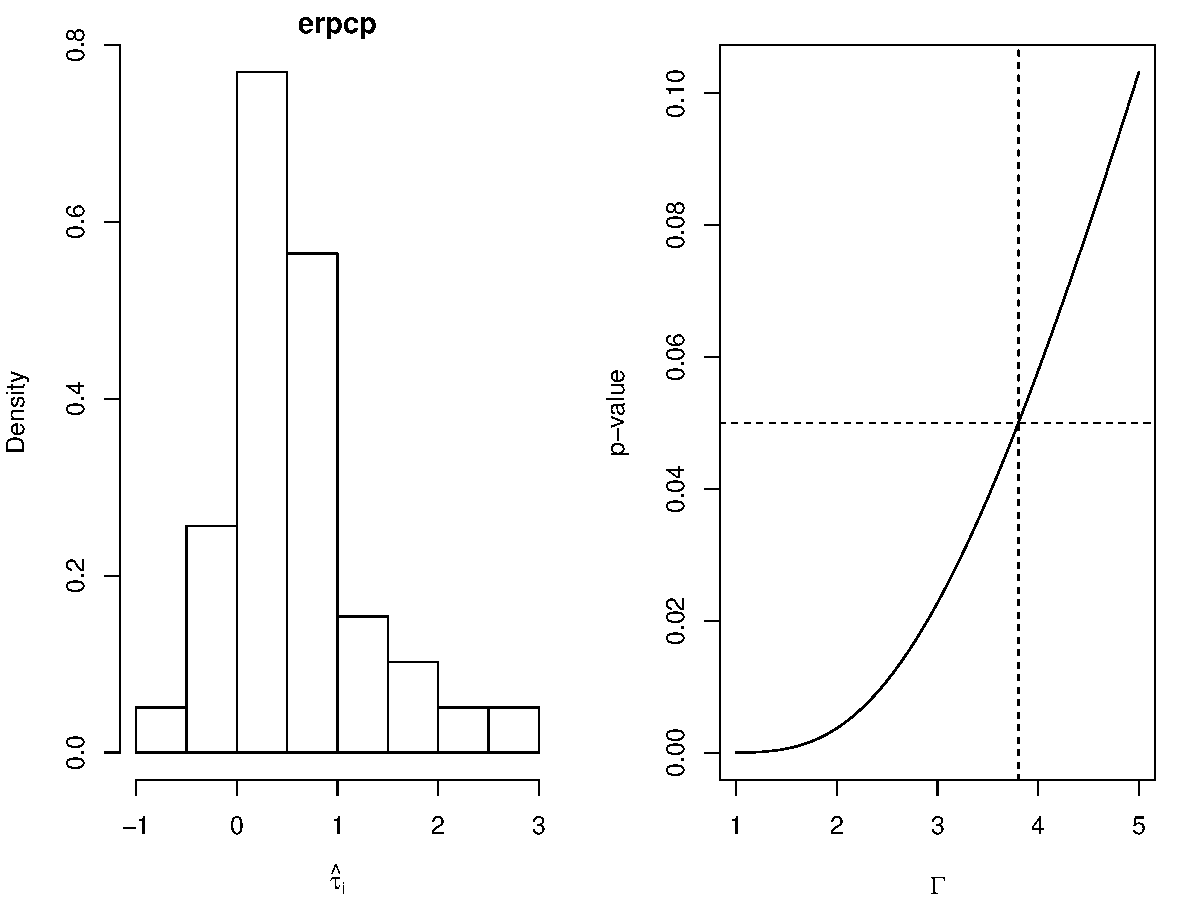
\includegraphics[width=\textwidth]{figures/erpcp_p_gamma.pdf}
                \caption{erpcp数据}
                \label{fig::erpcp}
        \end{subfigure}%
        
        
        
        
        
        
\begin{subfigure}[b]{\textwidth}
                \centering
                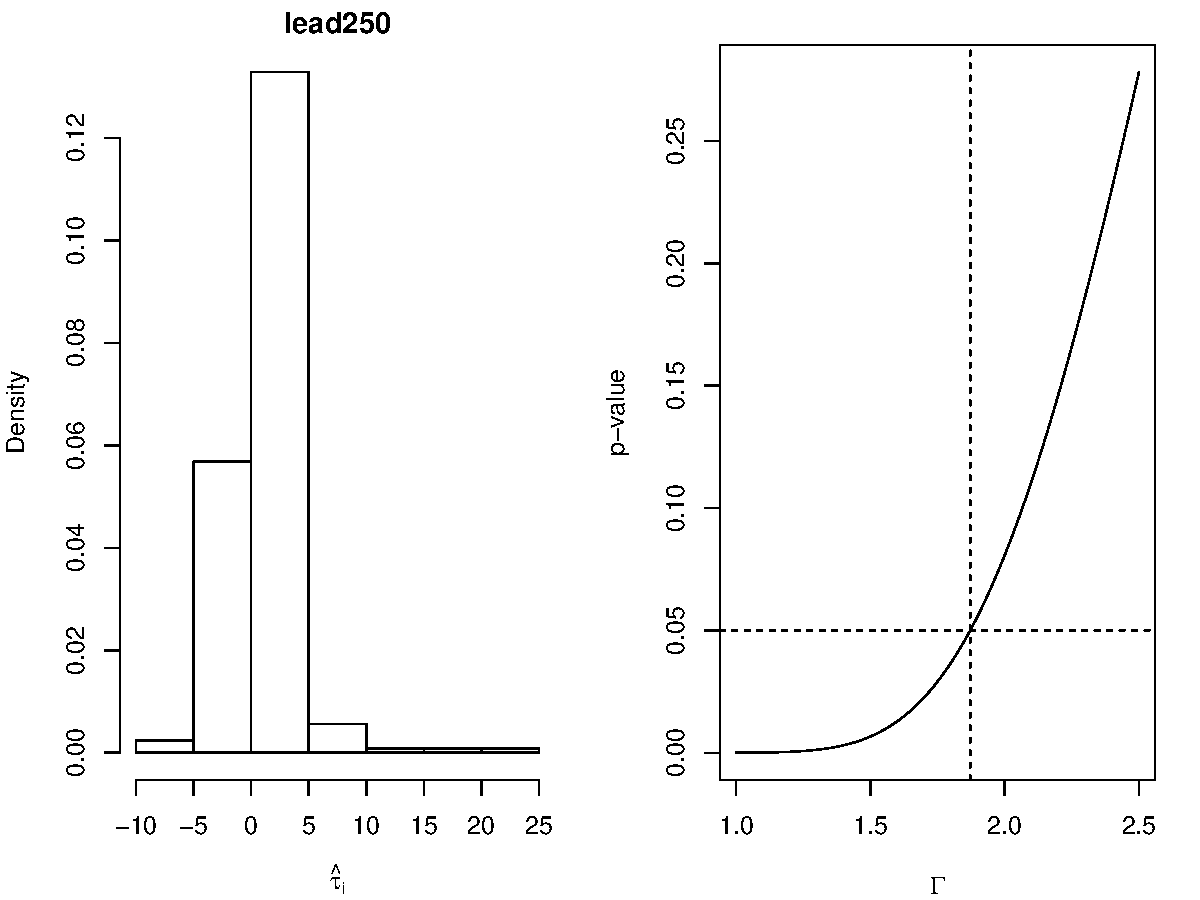
\includegraphics[width=\textwidth]{figures/lead250_p_gamma.pdf}
                \caption{ead250数据}
                \label{fig::ead250}
        \end{subfigure}%        
\caption{两个实例：$\hat{\tau}_i$分布直方图与$p$值随$\Gamma$的变化。}\label{fg::another2sensitivity}
\end{figure}


 
  

\section{作业习题}


\paragraph{假设\ref{assume::rosenbaum-sensitivity}的等价形式}\label{hw::rosenbaum-equivalent}

假设\ref{assume::rosenbaum-sensitivity}存在如下等价表述： 


\begin{assumption}
\label{assume::rosenbaum-equivalent}
倾向得分服从如下模型：
$$
\log \frac{  \pi_{ij} }{  1-\pi_{ij}  } = g(X_i) + \gamma U_{ij} ,\quad (i=1,\ldots, n; j=1,2)
$$
其中$g(\cdot)$为未知函数，$U_{ij} \in [0, 1]$为个体$(i, j)$的未观测协变量。 
\end{assumption}


证明：若假设\ref{assume::rosenbaum-equivalent}成立，则取$\Gamma = e^\gamma$时，假设\ref{assume::rosenbaum-sensitivity}必然成立。 


注：\citet[][page 108]{rosenbaum2002design}还证明，若假设\ref{assume::rosenbaum-sensitivity}成立，则存在一组$U_{ij}$使假设\ref{assume::rosenbaum-equivalent}成立。假设\ref{assume::rosenbaum-equivalent}可能更容易解释，因为$\gamma$衡量$U$对处理的条件对数优势比；逻辑回归系数的解释见第\ref{sec::logistic-regression}节。 



\paragraph{Rosenbaum方法的实践应用}
试运用基于配对的Rosenbaum法重新分析实例\ref{eg::chan-bmi-ATE}。



\paragraph{推荐阅读}


\citet{rosenbaum2015two}详细介绍了其开发的两个用于配对观察性研究敏感性分析的\ri{R}语言包使用教程。 

  
    
\chapter{观察性研究中的重叠现象：难点与机遇}
  \label{chapter::overlap}


 
\section{重叠现象的影响}

在本书的 \ref{part::observational-studies} 部分中，基于观察性研究的因果推断依赖于两个关键假设：可忽略性  
$$
Z\ind \{ Y(1), Y(0)  \} \mid X
$$
以及重叠性  
 $$
 0 <  e(X) <  1 .
 $$ 
 \citet{d2017overlap} 指出这两个假设之间存在矛盾：通常而言，更多的协变量会让可忽略性假设更容易成立（此处暂不考虑 \ref{section::m-bias} 中所讨论的M偏差问题），但更多的协变量又会降低重叠性假设的成立可能性，因为此时治疗分配变得更加可预测。 

若某些单位满足$e(X) = 0$或$e(X) = 1$，那么在理解其反事实潜在结果时就存在概念上的困难\citep{king2006dangers}。特别地，如果一个单位必然接受处理，设想它在对照下的潜在结果可能没有意义；如果它必然接受对照，设想它在处理下的潜在结果也可能没有意义。即使真实倾向得分并非恰好等于$0$或$1$，有限样本中的估计倾向得分也可能非常接近$0$或$1$，从而使基于IPW的估计量数值不稳定。第\ref{chapter::pscore-key}章已讨论过这个问题。 


实际上，许多统计分析都需要满足一种更严格的重叠性条件：

\begin{assumption}
[严格重叠性]
\label{assume::strong-overlap}
对于某个$\eta \in (0,1/2).$，有$\eta \leq e(X) \leq 1-\eta$
\end{assumption}


然而，\citet[][Corollary 1]{d2017overlap}表明，当协变量很多时，假设\ref{assume::strong-overlap}蕴含很强的限制。为简便起见，这里只介绍他们的一个结果。记$X_k\ (k=1,\ldots, p)$为协变量$X = (X_1, \ldots, X_p)$的第$k$个分量，记$$
e= \pr(Z=1)
$$为处理单位所占比例。 


\begin{theorem}\label{thm::overlap-implications}
假设\ref{assume::strong-overlap}蕴含$\eta \leq e \leq 1-\eta$及\begin{eqnarray} 
&&p^{-1} \sum_{k=1}^p \big | E(X_k\mid Z=1) - E(X_k\mid Z=0)  \Big |   \nonumber  \\
& \leq &  
p^{-1/2} C^{1/2}  \left\{    e\lambda_1^{1/2} + (1-e)  \lambda_0^{1/2}  \right\} , \label{eq::mean-balance-overlap}
\end{eqnarray}其中$$
C  = \frac{  (e-\eta)(1-e-\eta)   }{  e^2(1-e)^2 \eta (1-\eta)      }
$$是仅依赖$(e, \eta)$的正常数，$\lambda_1$和$\lambda_0$分别为协方差矩阵$ \cov(X\mid Z=1)$和$\cov(X\mid Z=0) $的最大特征值。 
\end{theorem}

定理\ref{thm::overlap-implications}中最大特征值的阶是多少？\citet{d2017overlap}指出，除非$X$的各分量高度相关，否则其阶通常小于$O(p)$。若$X$各分量高度相关，在纳入其他分量后，一些分量就是冗余的。若$X$各分量并非高度相关，则右端趋于零。因此，在所有协变量维度上平均而言，两组的均值差接近零，即处理组和对照组在平均意义上近乎均值平衡。从数学上看，\eqref{eq::mean-balance-overlap}左端趋于零，排除了$X$的所有维度在两组间均具有不消失的均值差的可能性。这对含有很多协变量的观察性研究是很强的要求。 



\subsection{重叠性不足情况下的修剪处理}\label{sec::trimming-overlap}

当假设\ref{assume::strong-overlap}不成立时，常根据估计倾向得分进行修剪\citep{crump2009dealing, yang2018asymptotic}。修剪剔除重叠很少区域内的单位，从而改变目标总体和目标估计参数。假设\ref{assume::strong-overlap}中重叠性所隐含的严格限制表明，在高维情形下可能必须更频繁地修剪，并可能需要剔除很大一部分单位，才能达到理想的重叠程度。 


\subsection{重叠性不足情况下的结果建模}\label{sec::outcome-modeling-overlap}


\citet{d2017overlap} 所得到的结果也在一定程度上揭示了：在重叠性不足时仅关注倾向得分的做法存在局限性。这在某种意义上也是对 \citet{rubin2008objective} 提出的“就客观的因果推断而言，实验设计比统计分析更重要”这一观点的挑战。\citet{rubin2008objective} 极其强调观察性研究中的“设计”阶段的重要性，而该阶段的核心正是倾向得分，可惜在协变量数量较多时倾向得分往往难以满足重叠性条件。 



当面对高维协变量时，结果建模的重要性便凸显出来。特别地，若结果变量的均值仅依赖于原始协变量经某种变换后得到的函数，即满足
$$
E\{  Y(z) \mid X \} = f_z( r(X)   ),\quad (z=0,1)
$$
那么只需控制 $r(X)$ 这一低维概括量即可。更多细节请参见 \ref{hw::outcome-modeling-overlap} 习题。由于实现了降维处理，此时针对 $r(X)$ 的重叠性条件往往要比针对 $X$ 的条件宽松得多。这一思路虽直观易懂，但目前尚缺相应的理论支持与实现方法。 



\section{无重叠情况下的因果推断：回归间断设计}
\label{sec::rdd}

先考虑$X$为一维的简单情形。一种极端的处理分配机制是确定性的：$$
 Z = I(X \geq x_0),
$$其中$x_0$为预先确定的阈值。这种分配有一个有趣的结果：可忽略性自动成立，$$
Z\ind \{  Y(1), Y(0) \} \mid X
$$因为$Z$是$X$的确定性函数，而常数与任何随机变量独立。然而，根据定义，重叠性遭到违反：$$
e(X) = \pr(Z=1\mid X) = 1(X \geq x_0)
=\begin{cases}
1 & \text{ if } X \geq x_0, \\
0& \text{ if }  X < x_0.
\end{cases}
$$因此，第\ref{part::challenges-os}部分讨论的分析策略不再适用，必须换一个角度。  


上述确定性处理分配似乎是人为构造的，但它在实践中有很多应用，称为{\it 断点回归}。下面先介绍几个经典例子，再给出这类研究的数学表述。 


\subsection{实例与图形诊断法}
\label{sec::rdd-examples}


\begin{example}
\citet{thistlethwaite1960regression}最早提出{\it 断点回归分析}的思想。他们研究的例子是学生获得优秀证书对其后续职业规划的影响。是否获证由奖学金资格考试成绩是否超过某个阈值决定。他们最初主要进行图形分析，图\ref{fig::thistlethwaite1960regression}展示了其中一幅图。 
\end{example}

\begin{figure}
\centering
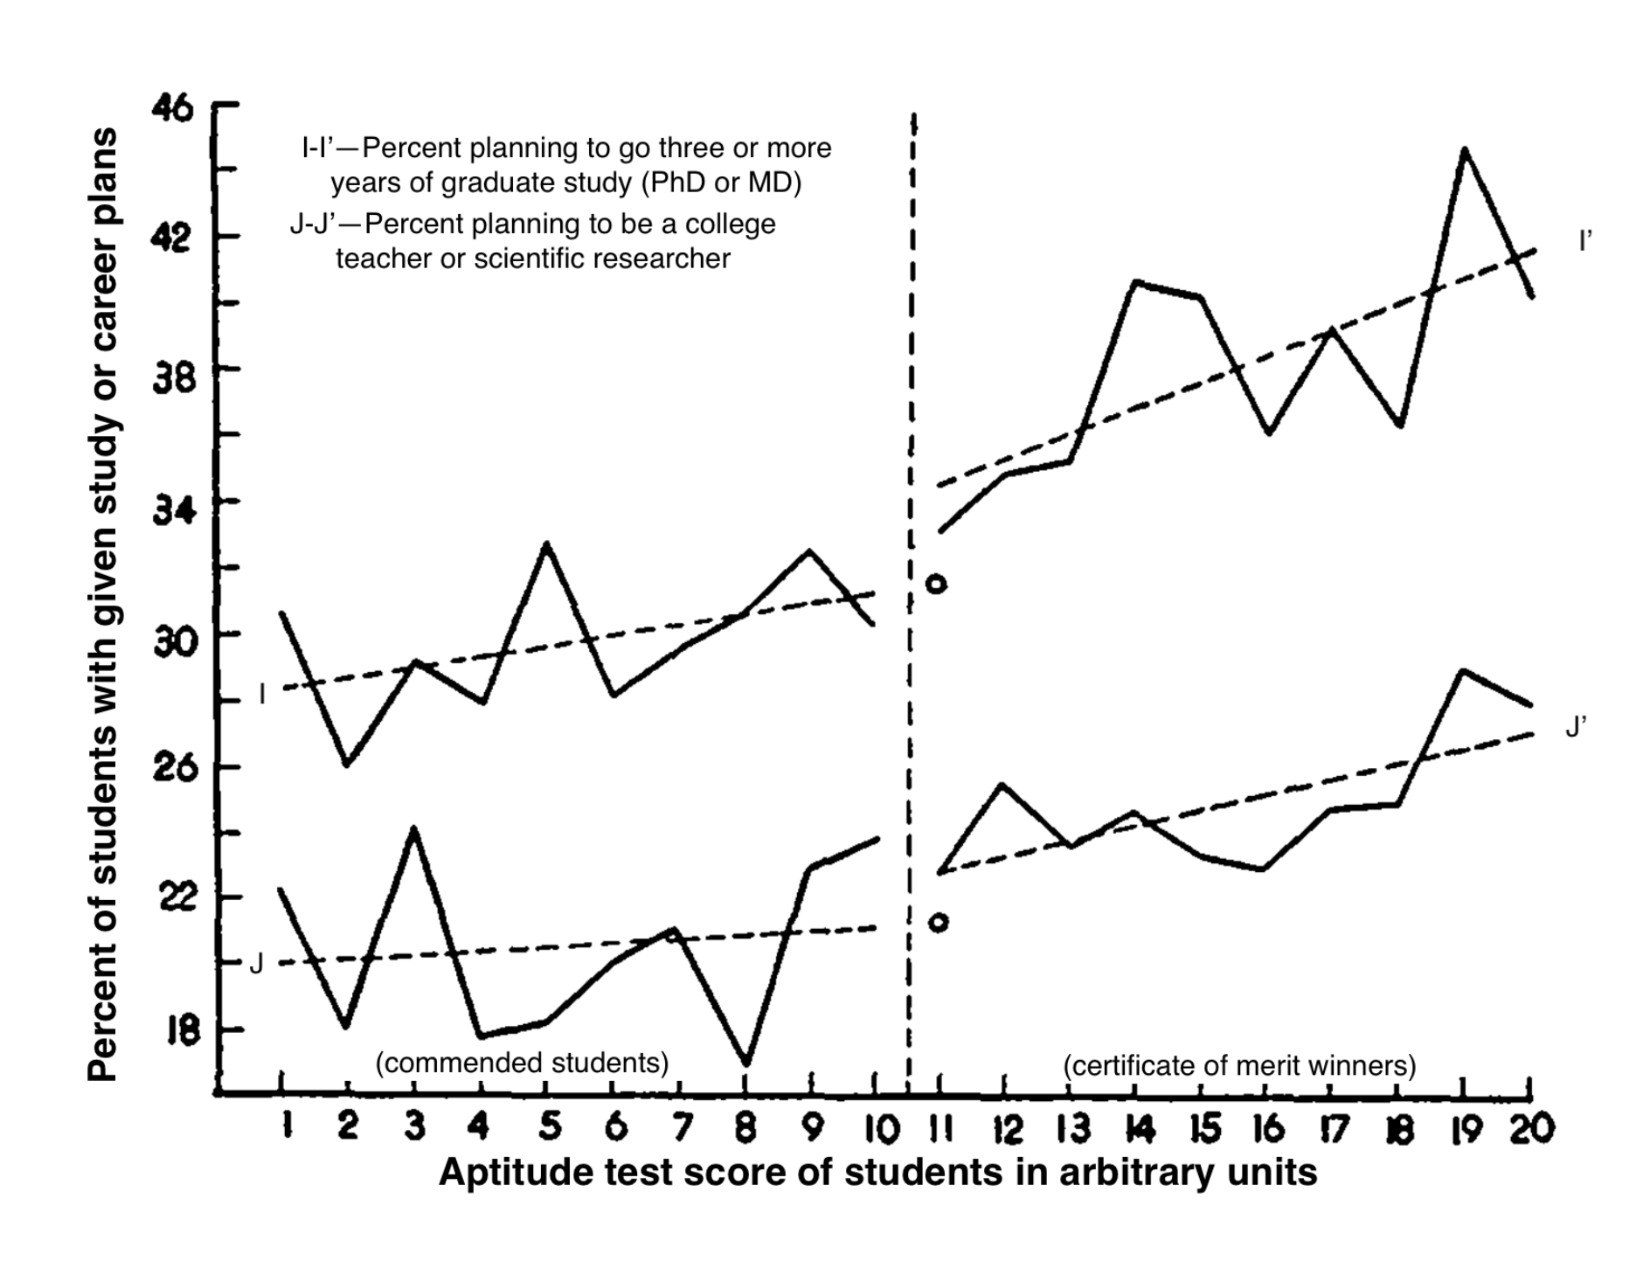
\includegraphics[width = \textwidth]{figures/rdd_graph_1960_modified.pdf}
\caption{改编自 \citet{thistlethwaite1960regression} 的图表，原文中部分文字表述不清，此处略有修改}\label{fig::thistlethwaite1960regression}
\end{figure}

 


\begin{example}
\citet{bor2014regression}使用断点回归研究HIV患者开始抗逆转录病毒治疗的时机对死亡率的影响。是否治疗由患者的CD4计数是否低于200个细胞/$\mu$L决定。CD4细胞是对抗感染的白细胞。
\end{example}




\begin{example}
\citet{carpenter2009effect} 研究了饮酒行为对死亡率的影响，他们以法定最低饮酒年龄作为饮酒行为的“间断点”。该研究所用数据源自美国国家健康统计中心，包含死亡者的出生日期与死亡日期。作者计算了每10万人生存年数中的死亡率，并选用了以下九个变量作为观测指标：
\begin{tabular}{cc}
\hline 
\texttt{all} & 全部死亡案例，即 \texttt{internal} 与 \texttt{external} 之和\\
\texttt{internal} & 因内部原因导致的死亡\\
\texttt{external} & 因外部原因导致的死亡，其余各类死亡因素之和\\
\texttt{homicide} & 他杀 \\
\texttt{suicide} & 自杀\\
\texttt{mva} & 机动车事故致死\\
\texttt{alcohol} & 死亡说明中提及饮酒因素者\\
\texttt{drugs} & 死亡说明中提及药物滥用因素者\\
\texttt{externalother} & 其他外部原因导致的死亡\\
\hline 
\end{tabular}


图 \ref{fig::mlda-9outcomes} 基于 \citet{angrist2014mastering} 所用的数据，呈现了九个指标在21岁阈值处的变化情况。从图中可明显看出，21岁之后死亡率显著上升，这主要源于机动车事故致死率的升高。具体的分析过程留作习题 \ref{hw::MLDA}。 
\end{example}
 

\begin{figure}
\centering
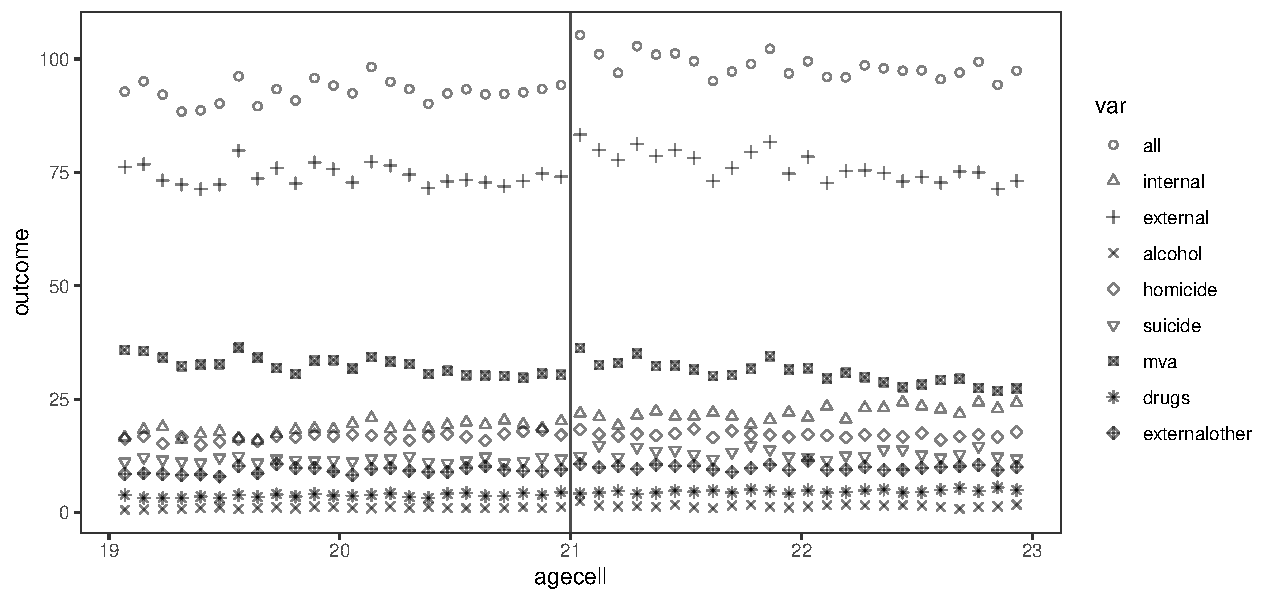
\includegraphics[width = \textwidth]{figures/mlda_9outcomes.pdf}
\caption{基于 \citet{carpenter2009effect} 数据的法定饮酒年龄效应示例}\label{fig::mlda-9outcomes}
\end{figure}


 

 



\subsection{回归间断设计的数学表述}


决定处理的变量$X$，其技术名称是{\it 运行变量}。直观上，断点回归可以识别阈值$x_0$处的{\it 局部平均因果效应}：$$
\tau(x_0) = E\{ Y(1) - Y(0)  \mid X=x_0 \}. 
$$特别地，对于处理下的潜在结果，有\begin{eqnarray}
E\{ Y(1) \mid X=x_0 \} &=& \lim_{\varepsilon \rightarrow 0+ } E\{ Y(1) \mid X=x_0+\varepsilon \} \label{eq::srd-continuity} \\
&=& \lim_{\varepsilon \rightarrow 0+} E\{ Y(1) \mid Z=1, X=x_0+\varepsilon \}  \label{eq::srd-z} \\
&=&  \lim_{\varepsilon \rightarrow 0+} E( Y \mid Z=1, X=x_0+\varepsilon ),
\end{eqnarray}其中若$ E\{ Y(1) \mid X=x\}$在$x_0$处右连续，便得到\eqref{eq::srd-continuity}；\eqref{eq::srd-z}则由$Z$的定义得到。类似地，若$ E\{ Y(0) \mid X=x\}$在$x_0$处左连续，则对照下的潜在结果满足$$
E\{ Y(0) \mid X=x_0 \} =  \lim_{\varepsilon \rightarrow 0+} E( Y \mid Z=0, X=x_0-\varepsilon )
$$因此，可以用这两个极限之差识别$x_0$处的局部平均因果效应。下面总结这一关键识别结果。


\begin{theorem}
\label{thm::identification-rdd}
假设治疗分配规则为 $Z = I(X \geq x_0)$，其中 $x_0$ 为预先设定的阈值。  
再假设 $ E\{ Y(1) \mid X=x\}$ 在 $x_0$ 处右连续，且 $ E\{ Y(0) \mid X=x\}$ 在 $x_0$ 处左连续。此时 $X=x_0$ 处的局部平均处理效应可由下式识别：
$$
\tau(x_0) = \lim_{\varepsilon \rightarrow 0+} E( Y \mid Z=1, X=x_0+\varepsilon ) - \lim_{\varepsilon \rightarrow 0+} E( Y \mid Z=0, X=x_0-\varepsilon ).
$$
\end{theorem}

由于上述公式右侧仅涉及可观测变量，因此参数 $\tau(x_0)$ 可通过非参数方法得以识别。不过该识别公式的形式与我们之前推导出的形式截然不同：这里涉及的是两个条件期望函数的极限值。 



\subsection{阈值附近区域的回归分析}\label{sec::rdd-numerical}

运气较好的话，图形诊断法有时也能清晰呈现阈值处的因果效应。不过多数实际观测数据均存在波动，因此仅凭图形诊断在有限样本下仍显不足。图 \ref{fig::4examples-rdd} 展示了四个模拟示例：前两例在阈值处呈现明显跳跃，后两例则无明显跳跃，不过所有示例的数据生成机制均包含阈值间断特性。 

\begin{figure}
\centering
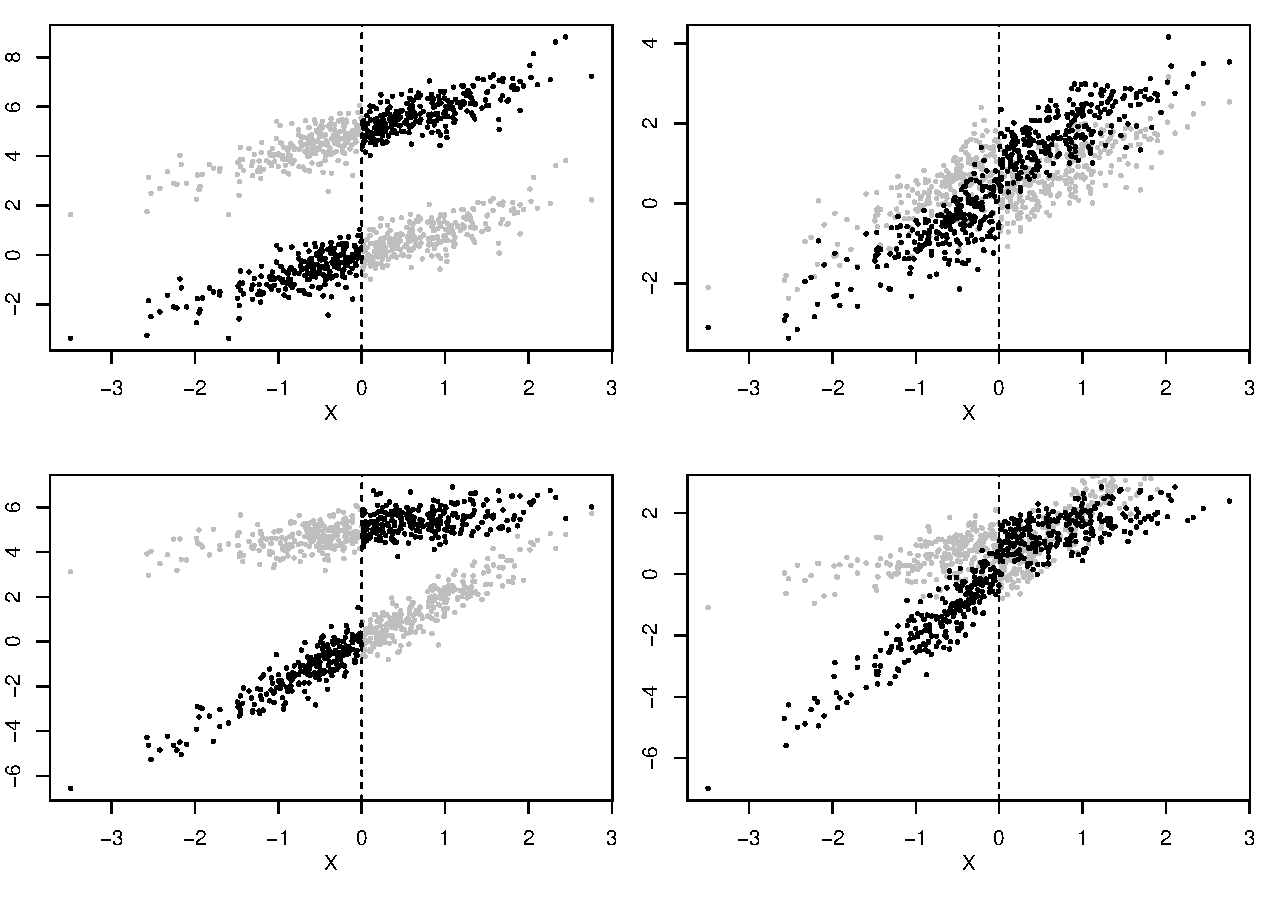
\includegraphics[width = \textwidth]{figures/rdd_graph.pdf}
\caption{断点回归示例。黑点为观测结果，灰点为未观测的反事实结果。第一列的数据生成过程在阈值处产生明显跳跃，第二列的跳跃则不明显。第一行的数据生成过程具有恒定的$\tau(x)$；第二行的$\tau(x)$随$x$变化。}\label{fig::4examples-rdd}
\end{figure}



假设 $E( Y \mid Z=1, X=x ) = \gamma_1 + \beta_1 x$ 与 $E( Y \mid Z=0, X=x ) = \gamma_0 + \beta_0 x $ 是关于 $x$ 的线性函数。此时我们可分别基于治疗组与对照组数据运行最小二乘回归，得到拟合直线 $\hat\gamma_1 + \hat\beta_1 x$ 与 $\hat\gamma_0 + \hat\beta_0 x$。进而可计算 $X = x_0$ 处的平均处理效应估计值：
$$
\hat\tau(x_0) = (\hat\gamma_1 -\hat\gamma_0 ) + (\hat\beta_1 -\hat\beta_0) x_0 .
$$
从数值上而言，$\hat\tau(x_0) $ 与在以下最小二乘回归模型中 $Z_i$ 的系数完全一致：
\begin{eqnarray}
Y_i \sim \{ 1, Z_i, X_i - x_0, Z_i (X_i - x_0)  \} , \label{eq::ols-rdd-1}
\end{eqnarray}
同样的值也对应着下面这个回归模型中 $Z_i$ 的系数：
\begin{eqnarray}
Y_i \sim \{ 1, Z_i,  R_i, L_i \},\label{eq::ols-rdd-2}
\end{eqnarray}
此处 
$$
R_i = \max(X_i - x_0, 0) ,\qquad L_i= \min (X_i - x_0, 0)
$$ 
分别代表了 $X_i - x_0$ 的正负值部分。具体代数推导过程留作习题 \ref{hw::rdd-ols-fits} 讨论。


不过，这种方法可能对违反线性模型假设较为敏感。理论建议只使用阈值附近的局部观测进行回归\footnote{在非参数统计中，这称为{\it 局部线性回归}，属于更广泛的{\it 局部多项式回归}方法\citep{fan2018local}。}。然而，如何选取“局部观测”的规则相当复杂。所幸\ri{R}中\ri{rdrobust}包的\ri{rdrobust}函数实现了多种选择。由于局部观测的选择是断点回归的关键，报告多种选择下的估计值和置信区间似乎更合理。这可视为断点回归的敏感性分析。 


\subsection{实例演示}
\label{section::lee-RDD-example}

\citet{lee2008randomized} 提供了一个著名案例：利用回归间断设计研究美国众议院选举中现任议员的优势所在。  
作者指出：“顾名思义，现任议员即指在上次选举中获胜的政治家。若使其获胜的因素具有相对持续性，那么他们再度当选的可能性理应更高。”由此可见，这确实是一个极具挑战性的因果推断问题。而回归间断设计则堪称研究此类问题的精巧方案。 



运行变量是上一次选举的得票率，并将其中心化到$0$；结果是本次选举的得票率，研究单位为国会选区。处理变量表示某政党是否为该选区当前的执政党，由上次选举的得票情况决定。以下\ri{R}代码生成展示原始数据的图\ref{fig::lee2008}。 

\begin{lstlisting}
house = read.csv("house.csv")[, -1]
plot(y ~ x, data = house, pch = 19, cex = 0.1)
abline(v = 0, col = "grey")
\end{lstlisting}

\begin{figure}
\centering
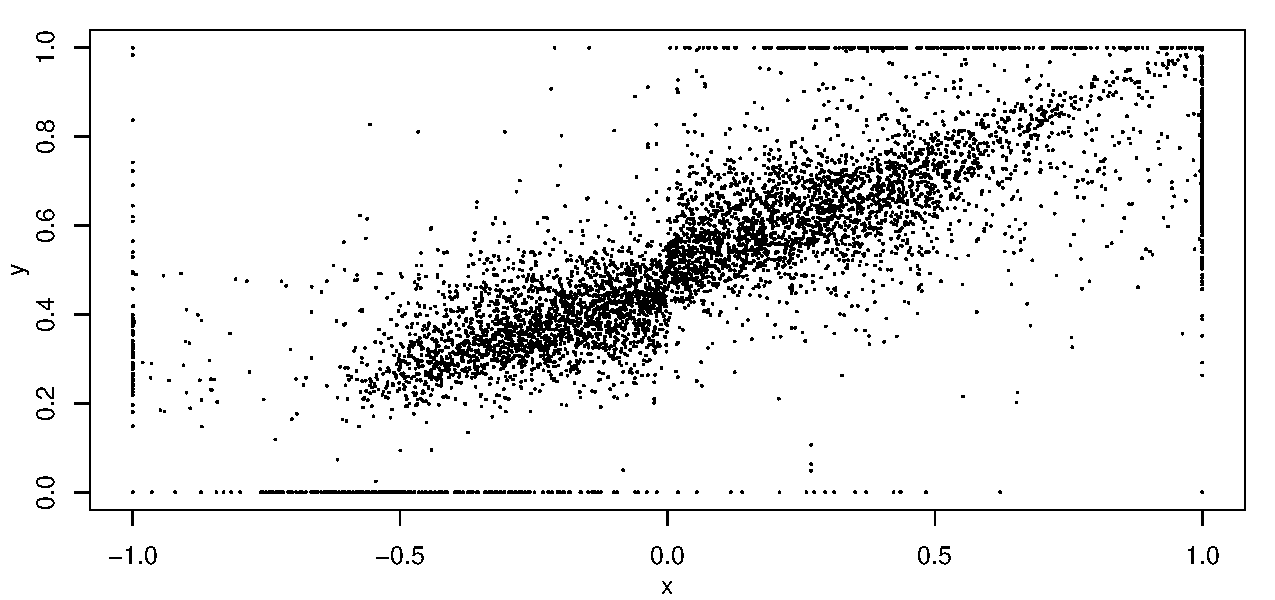
\includegraphics[width = \textwidth]{figures/lee2008rdd.pdf}
\caption{基于 \citet{lee2008randomized} 数据的原始分布图}\label{fig::lee2008}
\end{figure}

 
\ri{rdrobust} 函数可给出三组点估计值与置信区间，均显示现任议员具有显著优势。 

\begin{lstlisting}
> library(rdrobust)
> RDDest = rdrobust(house$y, house$x)
Warning message:
In rdrobust(house$y, house$x) :
  Mass points detected in the running variable.
> cbind(RDDest$coef, RDDest$ci)
                    Coeff   CI Lower   CI Upper
Conventional   0.06372533 0.04224798 0.08520269
Bias-Corrected 0.05937028 0.03789292 0.08084763
Robust         0.05937028 0.03481238 0.08392818
\end{lstlisting}
 
 
 
以下\ri{R}代码还可在按$|X| < h$定义的不同局部观测范围内，通过OLS得到点估计和置信区间。
\begin{lstlisting}
house$z = (house$x >= 0)
hh = seq(0.05, 1, 0.01)
local.lm = sapply(hh, function(h){
  Greg = lm(y ~ z + x + z*x, data = house,
            subset = (abs(x)<=h))
  cbind(coef(Greg)[2], confint(Greg, 'zTRUE'))
})
plot(local.lm[1, ] ~ hh, type = "p",
     pch = 19, cex = 0.3,
     ylim = range(local.lm),
     xlab = "h",
     ylab = "point and interval estimates",
     main = "subset linear regression: |X|<h")
lines(local.lm[2, ] ~ hh, type = "p",
      pch = 19, cex = 0.1) 
lines(local.lm[3, ] ~ hh, type = "p",
      pch = 19, cex = 0.1)
\end{lstlisting}
图 \ref{fig::rdd-lee} 展示了上述估计结果与置信区间随 $h$ 的变化情况。尽管估计值及区间范围对 $h$ 的取值较敏感，但定性结论仍与前述结果一致。 
 
\begin{figure}[h]
\centering
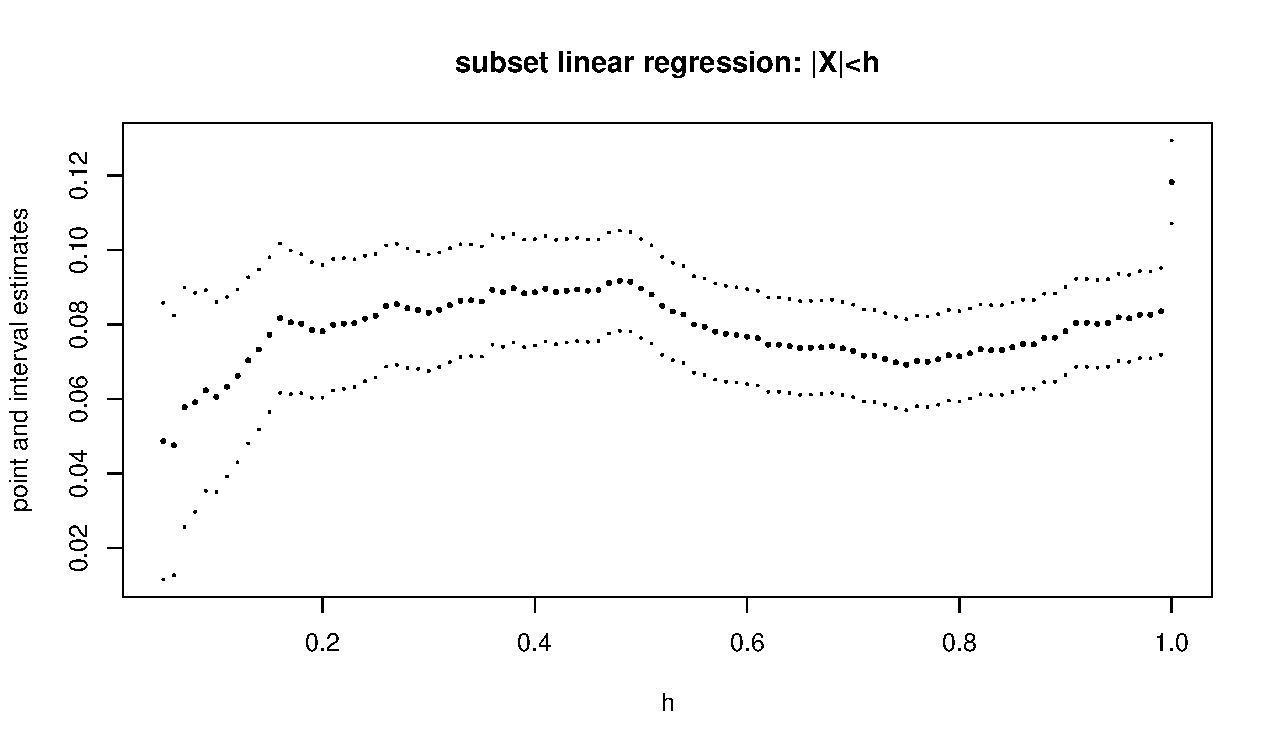
\includegraphics[width = \textwidth]{figures/rdd_lee.pdf}
\caption{基于局部线性回归的估计值与置信区间}\label{fig::rdd-lee}
\end{figure} 
 
 
 
\subsection{回归间断设计的局限性}\label{sec::problems-RD}


回归间断分析可能遇到哪些问题呢？首要的技术难点便是如何精准界定阈值附近的“邻域”。上文已提及此点。

此外，定理 \ref{thm::identification-rdd} 的成立依赖于连续性条件，而现实中该条件可能并不满足。举例来说，若21岁这一阈值处死亡率出现跳跃，则我们未必能将图 \ref{fig::mlda-9outcomes} 中的变化完全归因于法定饮酒年龄调整引发的饮酒行为改变。遗憾的是，这种连续性条件的违背现象很难通过实证方法加以检验。
 
 
\citet{mccrary2008manipulation}提出一种间接检验断点回归有效性的方法，即检查运行变量在阈值处的密度。若其密度在阈值处不连续，可能表明某些单位能够精确操控自身的处理状态。\ri{R}的\ri{rdd}包中，\ri{DCdensity}函数实现了这一检验，细节从略。 


 
 
\section{作业习题}

 

\paragraph{重叠性不足时结果建模的作用定理}\label{hw::outcome-modeling-overlap}

本题是对 \ref{sec::outcome-modeling-overlap} 内容的延伸探讨。我在此陈述一个正式定理。

\begin{theorem}
\label{thm::outcome-overlap}
假设 
$$
Z\ind Y(z) \mid X, \quad (z=0,1)
$$
且
$$
E\{  Y(z) \mid X \} = f_z( r(X)   ),\quad (z=0,1)
$$
其中 $r(X)$ 为某个确定的函数。  
此时平均因果效应 $\tau = E\{ Y(1) - Y(0)  \}$ 可通过以下两式识别：
$$
\tau =E\{   E(Y\mid Z=1, r(X)) - E(Y\mid Z=0, r(X)) \} 
$$
或
$$
\tau = E\left\{   \frac{ZY}{  e(r(X)) }  \right\}  - E\left\{   \frac{(1-Z)Y}{ 1 -  e(r(X)) }  \right\}
$$
此处 $e(r(X)) = \pr\{ Z=1\mid r(X) \}$。 
\end{theorem}

请证明定理 \ref{thm::outcome-overlap}。

说明：当$r(X) = X$时，定理\ref{thm::outcome-overlap}化为平均因果效应的标准IPW公式。当$r(X)$的维度低于$X$时，若$e(X)$的重叠条件不成立、而$e(r(X)) $的重叠条件仍成立，定理\ref{thm::outcome-overlap}就具有更广泛的适用性。 




 \paragraph{线性潜在结果模型}\label{hw::rdd-ols-fits}
 
 
 本题是对 \ref{sec::rdd-numerical} 中数值等价的进一步阐释。 
 
 证明$\hat\tau(x_0) $等于OLS拟合\eqref{eq::ols-rdd-1}和\eqref{eq::ols-rdd-2}中$Z_i$的系数。 
 
% Assume that 
% $$
% Y_i(1) = \gamma_1 + \beta_1 X_i + \varepsilon_i(1),\quad
%  Y_i(0) = \gamma_0 + \beta_0 X_i + \varepsilon_i(0)
% $$
%with $ E\{\varepsilon_i(1) \mid X_i \} =  E\{\varepsilon_i(0) \mid X_i \} = 0$. First, express 
%$$
%\tau(x_0) = E\{ Y_i(1) - Y_i(0)\mid X_i = x_0 \} 
%$$ 
%in terms of the parameters in the above model, and then show that $\tau(x_0)$ can be unbiased estimated by the coefficient of $Z_i$ in the OLS fits of \eqref{eq::ols-rdd-1} or \eqref{eq::ols-rdd-2}.  


提示：先绘制以 $X_i$ 为横轴、$Z_i(X_i - x_0)$、$L_i$ 与 $R_i$ 为纵轴的图像会大有助益。最终结论可通过重新参数化最小二乘回归模型得以验证。 



\paragraph{回归间断设计的模拟分析}

图 \ref{fig::4examples-rdd} 中潜在结果均源自线性模型。现请改用非线性模型进行模拟，并比较不同点估计值与置信区间的表现，尤其关注估计值的偏差、方差以及置信区间的覆盖率等指标。 



\paragraph{法定最低饮酒年龄数据的再分析}\label{hw::MLDA}


图\ref{fig::mlda-9outcomes}展示了阈值处的跳跃。分析\citet{carpenter2009effect}的\ri{mlda.csv}数据。

\paragraph{\citet{lee2008randomized} 数据的鲁棒性再分析}\label{hw::lee2008-robust}

图 \ref{fig::rdd-lee} 呈现了基于同方差假设的置信区间。现请重新绘制图表，使其展示基于 EHW 标准误差的置信区间。 




\paragraph{推荐阅读}

\citet{d2017overlap} 深入探讨了高维协变量条件下重叠性所带来的影响。 

\citet{thistlethwaite1960regression}关于断点回归的原始论文作为\citet{thistlewaiteregression2016obs}再版，并附有许多富有洞见的评论。巧合的是，\citet{thistlethwaite1960regression}和\citet{Rubin:1974}都发表于{\it Journal of Educational Psychology}。
      
     

\part{工具变量}\label{part::instrumentalvariables}
   
\chapter{从实验角度理解工具变量法}
 \label{chapter::iv-experiment}



{\it 工具变量方法}是计量经济学中的有力工具，能够在处理与结果之间存在混杂时识别因果效应。它依赖一个满足特定条件的额外变量，即{\it 工具变量}（IV）。初学时，这些条件可能不易理解，使工具变量方法显得有些神奇。本章从鼓励设计出发，给出一种并不神秘的解释。这也再次呼应了\citet{dorn1953philosophy}的建议：规划观察性研究时，应始终问自己下面的问题。\footnote{第\ref{chapter::observational-studies}章已经引用过这段话。}
\begin{quote}
如果能够通过受控实验来完成研究，那么实验应当如何开展呢？
\end{quote} 
工具变量方法在实验中的对应问题是{\it 不依从}，它出现在{\it 鼓励设计}中\citep{zelen1979new, powers1984effects, holland1986statistics}。 



\section{激励设计与不遵从行为}

考虑一项单位编号为$i = 1,\ldots, n$的实验。令$Z_i$表示分配的处理，$1$表示处理、$0$表示对照；令$D_i$表示实际接受的处理，$1$表示处理、$0$表示对照。若某个单位$i$满足$Z_i \neq D_i$，就出现了不依从问题。不依从非常常见，尤其是在以人为实验单位的鼓励设计中。此时实验者不能强迫单位接受处理，只能鼓励其接受。令$Y_i$表示所关心的结果。 

考虑对$Z$进行完全随机化，暂不考虑协变量$X$。相对于分配水平$1$与$0$，实际接受处理的潜在取值为$\{  D_i(1), D_i(0) \}$，结果的潜在取值为$\{ Y_i(1), Y_i(0)  \}$。它们的观测值分别为$D_i = Z_i D_i(1) + (1-Z_i) D_i(0)$和$Y_i = Z_i Y_i(1) + (1-Z_i) Y_i(0)$。为简化记号，假设$\{  Z_i, D_i(1), D_i(0) ,Y_i(1), Y_i(0)  \}_{i=1}^n \iidsim \{  Z, D(1), D(0) ,Y(1), Y(0)  \}$，并在不致混淆时省略下标$i$。 


先从完全随机实验开始。 
\begin{assumption}[随机化]
\label{assume::random}
$Z\ind \{D(1), D(0) ,Y(1), Y(0)   \}$. 
\end{assumption}

随机化使$D$和$Y$上的平均因果效应可识别：
$$
\tau_D = E\{  D(1) - D(0) \} = E(D\mid Z=1) - E(D \mid Z=0)
$$
以及
$$
\tau_Y = E\{  Y(1) - Y(0) \} = E(Y\mid Z=1) - E(Y\mid Z=0).  
$$
可分别用简单均值差估计量$\hat{\tau}_D$与$\hat{\tau}_Y$估计$\tau_D$与$\tau_Y$。 


报告估计值$\hat{\tau}_Y$及其标准误，称为意向治疗（ITT）分析。它估计处理分配对结果的效应，假设\ref{assume::random}中的完全随机实验设计保证了这一分析的有效性。但它未必回答真正的科学问题，即实际接受的处理对结果有何因果效应。 




\section{潜在依从状态与效应}

\subsection{非参数识别}


遵循\citet{imbens1994identification}和\citet{angrist1996identification}，按联合潜在取值$U_i = \{  D_i(1), D_i(0) \}$对总体分层。由于$D$为二元变量，共有四种组合：
\begin{eqnarray*}
U_i=\left \{ \begin{array} {ll}
\at  , & \text{if} \hspace{2mm} D_i(1)=1 \hspace{2mm} \text{and} \hspace{2mm} D_i(0)=1; \\
\cp  , & \text{if} \hspace{2mm} D_i(1)=1 \hspace{2mm} \text{and} \hspace{2mm} D_i(0)=0; \\
\df  ,& \text{if} \hspace{2mm} D_i(1)=0 \hspace{2mm} \text{and} \hspace{2mm} D_i(0)=1; \\
\nt  , & \text{if} \hspace{2mm} D_i(1)=0 \hspace{2mm} \text{and} \hspace{2mm} D_i(0)=0,
\end{array}
\right.  
\end{eqnarray*}
其中“$\at$”表示始终接受者，“$\cp$”表示依从者，“$\df$”表示反向依从者，“$\nt$”表示从不接受者。由于不能同时观测$D_i(1)$与$D_i(0)$，$U_i$是描述单位$i$依从行为的潜变量。 


根据$U$，用全概率公式可将$Y$上的平均因果效应分解为四项：
\begin{eqnarray} 
\tau_Y &=& E\{ Y(1) - Y(0) \mid U=\at  \} \pr(U = \at )  \nonumber  \\
&&+ E\{ Y(1) - Y(0) \mid U=\cp   \} \pr(U = \cp ) \nonumber  \\
&&+ E\{ Y(1) - Y(0) \mid U=\df  \} \pr(U = \df ) \nonumber  \\
&&+ E\{ Y(1) - Y(0) \mid U=\nt  \} \pr(U = \nt ) . \label{eq::decompose-ate-y-cace}
\end{eqnarray}
因此，$\tau_Y $是四个潜在亚组效应的加权平均。下面详细考察这些潜在亚组。 



下面的假设\ref{assume::Mono}将\eqref{eq::decompose-ate-y-cace}中的第三项限制为零。 
\begin{assumption}[单调性]
\label{assume::Mono}
对所有$i$，$\pr(U_i = \df) = 0$，或等价地，$D_i(1)\geq D_i(0)$，即不存在反向依从者。 
\end{assumption}

在{\it 单侧不依从}情形下，假设\ref{assume::Mono}自动成立：分配到对照组的单位无法获得处理，即所有单位都满足$D_i(0) = 0$。在随机化下，假设\ref{assume::Mono}蕴含可检验的限制
\begin{equation}
\label{eq::test-mono}
\pr(D=1\mid Z=1) \geq \pr(D=1\mid Z=0).
\end{equation}
但假设\ref{assume::Mono}远强于不等式\eqref{eq::test-mono}：前者在个体层面对$D_i(1)$与$D_i(0)$施加限制，后者只限制其平均水平。不过，只要可检验的限制\eqref{eq::test-mono}成立，就不能用观测数据反驳假设\ref{assume::Mono}。 


下面的假设\ref{assume::ER}要求处理分配只能通过实际接受的处理影响结果，从而将\eqref{eq::decompose-ate-y-cace}中的第一项和最后一项限制为零。 
\begin{assumption}[排除限制]
\label{assume::ER}
对于满足$U_i=\at$的始终接受者和满足$U_i = \nt$的从不接受者，均有$Y_i(1) = Y_i(0)$。 
\end{assumption}


假设\ref{assume::ER}的等价表述是：对所有$i$，$D_i(1) =  D_i(0)$必然蕴含$Y_i(1) =  Y_i(0)$。它要求处理分配只有在改变实际接受的处理时，才可能改变结果。在双盲随机对照试验中，这从生物学上通常是合理的，因为结果只依赖实际接受的处理。\footnote{一般应尽量实施盲法，以避免安慰剂效应、患者预期等带来的偏差。双盲试验中医生和患者都不知道处理分配；单盲试验中患者不知道，而医生知道。有时双盲甚至单盲都无法实施，这类试验称为开放试验。}也就是说，若处理分配不改变实际接受的处理，就也不改变结果。若处理分配存在不经由实际接受处理而影响结果的{\it 直接效应}，该假设就可能被违反。\footnote{这里非正式地使用“直接效应”一词，详见后文第\ref{chapter::mediation}和\ref{chapter::cde}章。}例如，非双盲随机对照试验中，处理分配可能通过未知途径影响结果。 





在假设\ref{assume::Mono}与\ref{assume::ER}下，分解式\eqref{eq::decompose-ate-y-cace}只剩第二项：
\begin{eqnarray}
\label{eq::aceY}
\tau_Y  = E\{ Y(1) - Y(0) \mid U=\cp   \} \pr(U = \cp ).
\end{eqnarray}
类似地，$D$上的平均因果效应可分解为四项：
\begin{eqnarray*}
\tau_D &=& E\{ D(1) - D(0) \mid U=\at  \} \pr(U = \at ) \\
&&+ E\{ D(1) - D(0) \mid U=\cp   \} \pr(U = \cp ) \\
&&+ E\{ D(1) - D(0) \mid U=\df  \} \pr(U = \df ) \\
&&+ E\{ D(1) - D(0) \mid U=\nt  \} \pr(U = \nt )  \\
&=& 0\times \pr(U = \at ) 
+ 1 \times \pr(U = \cp ) 
+ (-1)\times   \pr(U = \df )
+ 0 \times  \pr(U = \nt ) ,
\end{eqnarray*}
在假设\ref{assume::Mono}下简化为
\begin{eqnarray}
\label{eq::aceD}
\tau_D  = \pr(U = \cp ) .
\end{eqnarray}
由\eqref{eq::aceD}，依从者比例$\pi_\cp = \pr(U = \cp)$等于处理分配对$D$的平均因果效应，后者在完全随机实验中可识别。虽然不能根据观测数据确定哪些单位是依从者，但可由\eqref{eq::aceD}识别他们在总体中的比例。结合\eqref{eq::aceY}与\eqref{eq::aceD}，得到以下结论。


\begin{theorem}
\label{thm::CACE-identification}
在假设 \ref{assume::Mono} 与 \ref{assume::ER} 成立时，若 $\tau_D \neq 0$，则有 
$$
E\{ Y(1) - Y(0) \mid U=\cp   \} = \frac{ \tau_Y  }{ \tau_D}
$$ 
\end{theorem}


 

参考 \citet{imbens1994identification} 与 \citet{angrist1996identification} 的定义，我们定义

\begin{definition}[CACE 或 LATE]\label{def::CACE}
定义 
$$
\tau_\cp  =  E\{ Y(1) - Y(0) \mid U=\cp   \}  
$$
为“遵从者平均因果效应”或“局部平均处理效应”。该量亦可用下式表达：
\begin{eqnarray*}
\tau_\cp  &=&  E\{ Y(1) - Y(0) \mid D(1) = 1 , D(0) = 0  \} \\
&=&    E\{ Y(1) - Y(0) \mid D(1)  >  D(0)    \} . 
\end{eqnarray*}
\end{definition}

CACE 是满足$ D(1) = 1 , D(0) = 0$的依从者中$Z$对$Y$的平均因果效应；在单调性下，依从者也等价于满足$ D(1)  >  D(0)$的单位。由定义\ref{def::CACE}，定理\ref{thm::CACE-identification}可改写为
$$
\tau_\cp  = \frac{ \tau_Y  }{ \tau_D} ,
$$
即 CACE 或 LATE 等于$Y$上的平均因果效应与$D$上的平均因果效应之比。在假设\ref{assume::random}下，进一步得到如下 CACE 识别结果。


\begin{corollary}
\label{corollary::identification-CACE}
在假设 \ref{assume::random} 至 \ref{assume::ER} 均成立时，有
$$
\tau_\cp = \frac{ E(Y\mid Z=1) - E(Y\mid Z=0) }{ E(D\mid Z=1) - E(D \mid Z=0) } .
$$
\end{corollary}


因此，在完全随机实验、单调性与排除限制假设下，CACE 可通过结果均值差与处理均值差之比来非参数地估计。 



\subsection{估计方法}
\label{sec::estimation-IV}


根据推论\ref{corollary::identification-CACE}，可用简单比值
$$
\hat{\tau}_\cp  = \frac{  \hat{\tau}_Y }{  \hat{\tau}_D  } ,
$$
估计$\tau_\cp$，这称为 Wald 估计量\citep{wald1940fitting}或工具变量估计量。上述讨论中，$Z$是$D$的工具变量。   



可用下面的直观推导得到方差估计量（见例\ref{thm::delta-method}）：
$$
\hat{\tau}_\cp - \tau_\cp  = ( \hat{\tau}_Y  -  \tau_\cp\hat{\tau}_D)/\hat{\tau}_D 
\approx  ( \hat{\tau}_Y  -  \tau_\cp\hat{\tau}_D)/ \tau_D 
= \hat{\tau}_A / \tau_D ,
$$
其中$\hat{\tau}_A$是调整后结果$A_i = Y_i -  \tau_\cp D_i$的均值差。因此，$\hat{\tau}_\cp$的渐近方差近似等于$\hat{\tau}_A$的方差除以$\tau_D^2$。方差估计分以下几步进行： 
\begin{enumerate}
%[(\thesection.1)]
\item
计算调整后的结果变量 $\hat{A}_i =  Y_i -  \hat{\tau}_\cp D_i\ (i=1, \ldots, n)$；

\item
计算 Neyman 型方差估计值：
$$
\hat{V}_{\hat{A}} = \frac{\hat{S}_{\hat{A}}^2(1)}{n_1} + \frac{\hat{S}_{\hat{A}}^2(0)}{n_0},
$$
其中 $\hat{S}_{\hat{A}}^2(1)$ 与 $\hat{S}_{\hat{A}}^2(0)$ 分别为实验组与对照组下 $\hat{A}_i $ 的样本方差； 

\item
最终得到方差估计值 $ \hat{V}_{\hat{A}} /  \hat{\tau}_D ^2 .$ 
\end{enumerate}


上述方差估计量的论证见习题\ref{problem::var-iv-estimate}。也可用自助法近似$\hat{\tau}_\cp $的方差。下面的函数计算点估计$\hat{\tau}_\cp $，以及基于公式$\hat{V}_{\hat{A}} $和自助法的标准误。 

\begin{lstlisting}
## IV point estimator
IV_Wald = function(Z, D, Y)
{
       tau_D = mean(D[Z==1]) - mean(D[Z==0])
       tau_Y = mean(Y[Z==1]) - mean(Y[Z==0])
       CACE  = tau_Y/tau_D
       
       c(tau_D, tau_Y, CACE)
}

## IV se via the delta method
IV_Wald_delta = function(Z, D, Y)
{
       est         = IV_Wald(Z, D, Y)
       AdjustedY   = Y - D*est[3]
       VarAdj      = var(AdjustedY[Z==1])/sum(Z) + 
                          var(AdjustedY[Z==0])/sum(1 - Z)
       
       c(est[3], sqrt(VarAdj)/abs(est[1]))
}

##IV se via the bootstrap
IV_Wald_bootstrap = function(Z, D, Y, n.boot = 200)
{
       est      = IV_Wald(Z, D, Y)
       
       CACEboot  = replicate(n.boot, {
         id.boot = sample(1:length(Z), replace = TRUE)
         IV_Wald(Z[id.boot], D[id.boot], Y[id.boot])[3]
       })
       
       c(est[3], sd(CACEboot))
}
\end{lstlisting}


在零假设$\tau_\cp = 0$下，可用$\hat{V}_Y /  \hat{\tau}_D ^2$近似方差，其中$\hat{V}_Y$是$Y$均值差的 Neyman 型方差估计。若真实的$\tau_\cp$不为零，这个方差估计量就不一致，因此适用于检验而非一般估计。不过，它揭示了 ITT 估计量与 Wald 估计量的关系。ITT 估计量$\hat{\tau}_Y$的估计标准误为$\sqrt{ \hat{V}_Y}$。Wald 估计量$ \hat{\tau}_Y / \hat{\tau}_D$相当于将 ITT 估计量乘以$1/\hat{\tau}_D > 1$，其绝对值更大，但估计标准误也扩大相同倍数。根据方差估计$\hat{V}_Y $和$\hat{V}_Y /  \hat{\tau}_D ^2$，$\tau_Y$与$\tau_\cp$的置信区间分别为
$$
\hat{\tau}_Y \pm z_{1-\alpha/2} \sqrt{ \hat{V}_Y}
$$
和
$$
\hat{\tau}_Y  / \hat{\tau}_D \pm z_{1-\alpha/2} \sqrt{ \hat{V}_Y}  / \hat{\tau}_D
= 
\left( \hat{\tau}_Y \pm z_{1-\alpha/2} \sqrt{ \hat{V}_Y}  \right) / \hat{\tau}_D 
$$
其中$z_{1-\alpha/2}$是标准正态分布的$1-\alpha/2$分位数。这两个区间给出相同的定性结论：要么都包含零，要么都不包含零。从这个意义上说，尽管工具变量分析更复杂，它提供的定性信息与对$Y$作 ITT 分析相同。  




\section{协变量的作用}

\subsection{完全随机实验中的协变量调整}

现在考虑带有协变量的完全随机实验，假设
$$
Z\ind \{ D(1), D(0), Y(1), Y(0), X \}.
$$
利用协变量$X$，可分别对$D$和$Y$计算\citet{lin2013}提出的估计量$\hat{\tau}_{D,\textsc{L}}$与$\hat{\tau}_{Y,\textsc{L}}$，从而得到$\hat{\tau}_{\cp, \textsc{L}} = \hat{\tau}_{Y,\textsc{L}} / \hat{\tau}_{D,\textsc{L}}$。可用自助法近似$\hat{\tau}_{\cp, \textsc{L}} $的渐近方差。下面的函数计算点估计$\hat{\tau}_{\cp, \textsc{L}} $及其自助法标准误。 
 
\begin{lstlisting}
## covariate adjustment in IV analysis
IV_Lin = function(Z, D, Y, X)
{
  X     = scale(as.matrix(X))
  tau_D = lm(D ~ Z + X + Z*X)$coef[2]
  tau_Y = lm(Y ~ Z + X + Z*X)$coef[2]
  CACE  = tau_Y/tau_D
  
  c(tau_D, tau_Y, CACE)
}


##IV_adj se via the bootstrap
IV_Lin_bootstrap = function(Z, D, Y, X, n.boot = 200)
{
  X         = scale(as.matrix(X))
  est       = IV_Lin(Z, D, Y, X)
  CACEboot  = replicate(n.boot, {
    id.boot = sample(1:length(Z), replace = TRUE)
    IV_Lin(Z[id.boot], D[id.boot], Y[id.boot], X[id.boot, ])[3]
  })
  
  c(est[3], sd(CACEboot))
}
\end{lstlisting}

\subsection{条件随机化或无偏观察性研究中的协变量处理}
\label{section::unconfounded-IV}

若随机化仅在给定协变量后成立，即
$$
Z\ind \{ D(1), D(0), Y(1), Y(0) \} \mid  X,
$$
就必须调整协变量以避免偏差。分析仍很直接，因为第\ref{part::observational-studies}部分已讨论了多种估计$ Z$对$D$和$Y$的效应的方法。将这些估计量代入比值公式$\hat{\tau}_\cp = \hat{\tau}_Y / \hat{\tau}_D$，再用自助法近似渐近方差即可。对应的点估计和方差估计的实现留作习题\ref{hw::iv-conditional-x}。 



\section{弱工具变量问题}

\subsection{模拟分析}
 
即使$\tau_D >0$，$\hat{\tau}_D$仍有正概率为零，因此$\hat{\tau}_\cp$的方差为无穷大（见习题\ref{problem::infinite-var-iv}）。此前正态近似中的方差并非$\hat{\tau}_\cp$本身的方差，而是其渐近分布的方差，这是一个微妙的技术区别。$ \tau_D$接近$0$时称为弱工具变量情形，此时比值估计量$\hat{\tau}_\cp = \hat{\tau}_Y / \hat{\tau}_D$的有限样本性质很差：$\hat{\tau}_\cp$存在有限样本偏差，渐近分布非正态，对应 Wald 型置信区间的覆盖性质也较差。\footnote{相关理论通常假定$\tau_D$与$n^{-1/2}$同阶。在这一渐近设定下，随着$n$趋于无穷，依从者比例趋于零，工具变量方法只能识别一个比例不断缩小的亚组的平均因果效应。这是为理论分析构造的设定，在实践中很难论证其合理性。下面不作这一假设。}在结果$Y$为二元变量的简单情形下，$\tau_Y$必介于$-1$与$1$之间，但$\hat{\tau}_\cp$未必介于$-1$与$1$之间。 
 

图\ref{fig::no-x-iv}和\ref{fig::x-iv}给出了不同$\pi_\cp$下，模拟所得$\hat{\tau}_\cp$与$\hat{\tau}_{\cp, \textsc{L}}$的直方图。具体数据生成过程见\ri{R}代码。当$\pi_\cp$等于$0.2$或$0.1$时，估计量$\hat{\tau}_\cp$和$\hat{\tau}_{\cp, \textsc{L}}$的分布都远非正态，基于渐近正态性的统计推断很难可靠。 

\begin{figure}
\centering 
\begin{subfigure}[b]{\textwidth}
                \centering
                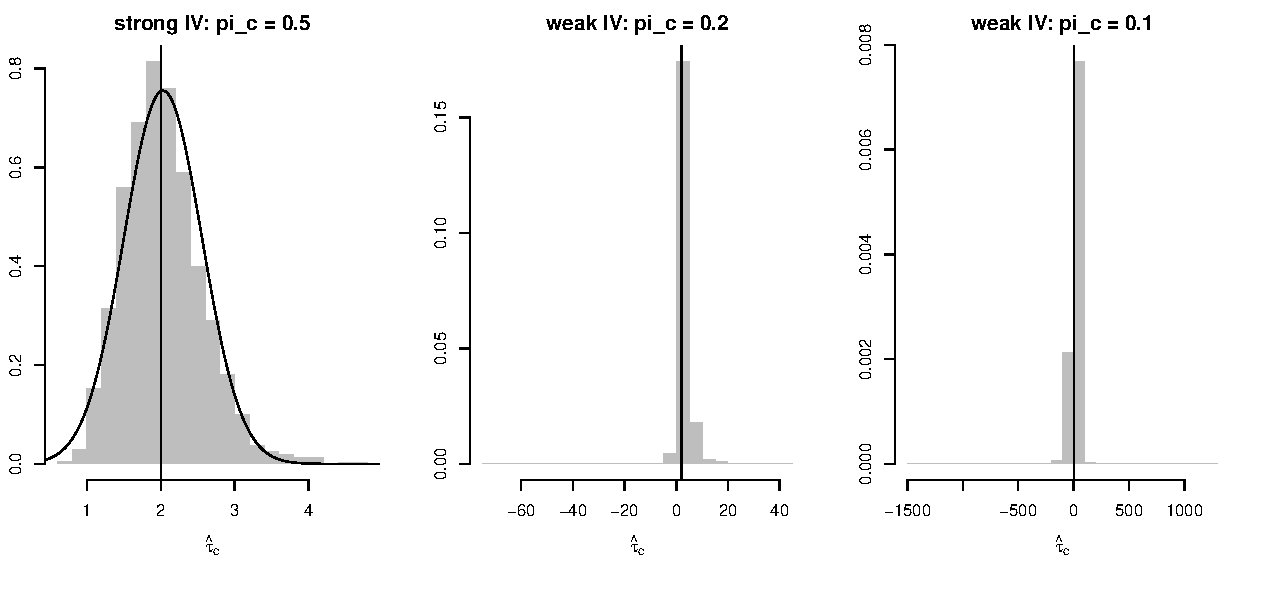
\includegraphics[width=\textwidth]{figures/wald_simulation.pdf}
                \caption{不进行协变量调整}
                \label{fig::no-x-iv}
        \end{subfigure}%
        
        
        
        
        
        
\begin{subfigure}[b]{\textwidth}
                \centering
                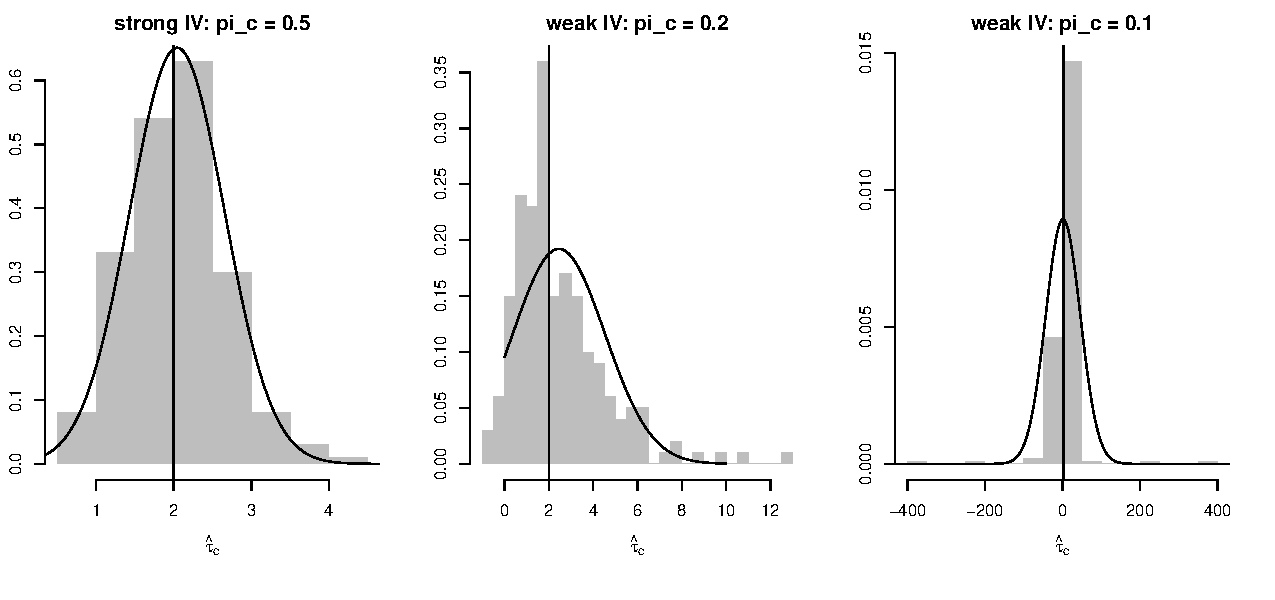
\includegraphics[width=\textwidth]{figures/waldX_simulation.pdf}
                \caption{进行协变量调整}
                \label{fig::x-iv}
        \end{subfigure}%        
\caption{强、弱工具变量的模拟}\label{fg::strong-weak-ivs}
\end{figure}


\subsection{鲁棒的置信区间构造}

如何处理弱工具变量？从检验角度看，解决办法很简单。由于$\tau_\cp = \tau_Y / \tau_D$，只要$\tau_D > 0$，下列两个零假设就等价：
$$
H_0: \tau_\cp  = 0 \Longleftrightarrow H_0': \tau_Y = 0
$$
因此，只需检验$H_0'$，即$Z$对$Y$的平均因果效应为零。这呼应了第\ref{sec::estimation-IV}节关于 ITT 分析与工具变量分析关系的讨论。 


从估计角度看，虽然点估计的有限样本性质较差，仍可以着重构造置信区间。由于$\tau_\cp = \tau_Y / \tau_D$，这个问题类似于经典的 Fieller--Creasy 问题。下面介绍受\citet{fieller1954some}启发的$\tau_\cp$置信区间构造方法，见第\ref{sec::fc-problem}节。利用置信区间与假设检验的对偶性（见第\ref{section::duality-ci-testing}节），可反演一系列零假设
$$
H_0(b): \tau_\cp = b . 
$$
来构造$\tau_\cp$的置信集合。在真实值$\tau_\cp = b$下，
$$
 \tau_Y  - b  \tau_D  = 0.
$$
所以零假设$H_0(b)$等价于结果$A_i( b) = Y_i - b  D_i $的平均因果效应为零：
$$
H_0(b): \tau_{A(b)} = 0 .
$$


令$ \hat{\tau}_A(b)$为$\tau_{A(b)} $的一般点估计量，$\hat{V}_A( b )$为对应方差估计量。其具体形式取决于研究设定。在不含协变量的完全随机实验中，$ \hat{\tau}_A(b)$是结果$A_i( b)$的均值差，$\hat{V}_A( b )$为 Neyman 型方差估计量。在含协变量的完全随机实验中，$ \hat{\tau}_A(b)$是\citet{lin2013}对结果$A_i( b)$提出的估计量，$\hat{V}_A( b )$是将$Y_i - b D_i$对$(Z_i, X_i, Z_i X_i)$作 OLS 回归得到的 EHW 方差估计，并加上第\ref{sec::cre-superpop}节讨论的修正项。\footnote{若采用有限总体视角，则不需要这个修正。}在无混杂观察性研究中，可以采用本书第\ref{part::observational-studies}部分的多种已有方法，估计$A_i( b)$上的平均因果效应及其方差。  


根据$ \hat{\tau}_A(b)$与$\hat{V}_A( b )$，可对$H_0(b)$构造 Wald 型检验。反演检验，就得到$\tau_\cp$的置信集合：
$$
\left\{  b:    \frac{   \hat{\tau}_A^2(b)  }{  \hat{V}_A(b)  } \leq z_{1-\alpha/2}^2 \right\}
$$
其中$z_{1-\alpha/2}$为标准正态分布的$1-\alpha/2$分位数。这与计量经济学中的 Anderson--Rubin 型置信区间\citep{anderson1950asymptotic}相近。考虑到它与\citet{fieller1954some}的联系，下面称其为 Fieller--Anderson--Rubin（FAR）置信区间。工具变量较强时，这些针对弱工具变量的区间退化为通常的渐近置信区间；工具变量较弱时，它们还能提供额外保证。我建议在实践中使用这些区间。 


\begin{example}\label{eg::FAR-CI-noX}
为直观理解 FAR 置信区间，考虑不含协变量的完全随机实验。区间中的二次不等式简化为
\begin{eqnarray*}
&& (\hat{\tau}_Y  - b   \hat{\tau}_D)^2 \\ 
& \leq & z_{1-\alpha/2}
\left[      n_1^{-1} \{  \hat{S}_Y^2(1)  + b^2\hat{S}_D^2(1) - 2 b \hat{S}_{YD}(1)  \}  \right. \\
&& \left. 
 + n_0^{-1} \{  \hat{S}_Y^2(0)  + b^2\hat{S}_D^2(0) - 2 b \hat{S}_{YD}(0)  \}    \right] ,
\end{eqnarray*}
其中$\{ \hat{S}_Y^2(1) ,  \hat{S}_D^2(1) , \hat{S}_{YD}(1)  \}$与$ \{ \hat{S}_Y^2(0), \hat{S}_D^2(0),\hat{S}_{YD}(0) \} $分别是处理组和对照组中$Y$、$D$的样本方差及协方差。置信集合可能是一个闭区间、两个不相连的区间、空集或整条实数轴。详细讨论留作习题\ref{para::FAR-CI-cases}。 
\end{example}
 



\subsection{实现与模拟}\label{sec::FARci-simulation}


下面的函数计算随$b$变化的一系列$p$值。\ri{FARci}不使用协变量，\ri{FARciX}使用协变量，后者依赖第\ref{sec::simulation-CRE-superp}节定义的\ri{linestimator}函数。 

\begin{lstlisting}
FARci = function(Z, D, Y, Lower, Upper, grid)
{
  CIrange = seq(Lower, Upper, grid)
  Pvalue  = sapply(CIrange, function(t){
    Y_t       = Y - t*D
    Tauadj    = mean(Y_t[Z==1]) - mean(Y_t[Z==0])
    VarAdj    = var(Y_t[Z==1])/sum(Z) + 
      var(Y_t[Z==0])/sum(1 - Z)
    Tstat     = Tauadj/sqrt(VarAdj)
    (1 - pnorm(abs(Tstat)))*2
  })
  
  return(list(CIrange = CIrange, Pvalue  = Pvalue))
}

FARciX = function(Z, D, Y, X, Lower, Upper, grid)
{
  CIrange = seq(Lower, Upper, grid)
  X       = scale(X)
  Pvalue  = sapply(CIrange, function(t){
    Y_t       = Y - t*D
    linest    = linestimator(Z, Y_t, X)
    Tstat     = linest[1]/linest[3]
    (1 - pnorm(abs(Tstat)))*2
  })
  
  return(list(CIrange = CIrange, Pvalue  = Pvalue))
}
\end{lstlisting}


图\ref{fg::FAR-ci-simulation}展示了不同$\pi_\cp$下模拟数据的$p$值随$b$变化的曲线。图\ref{fig::FARci-realization1}和\ref{fig::FARci-realization2}是同一数据生成过程的两次实现，细节见\ri{R}代码。图\ref{fig::FARci-realization1}中，FAR 置信集合都是闭区间；图\ref{fig::FARci-realization2}中，$\pi_\cp = 0.2$和$\pi_\cp = 0.1$时的置信集合则不是闭区间。$\pi_\cp = 0.5$时，置信集合的形状在两次实现中保持稳定。 



\begin{figure}
\centering 
\begin{subfigure}[b]{0.45\textwidth}
                \centering
                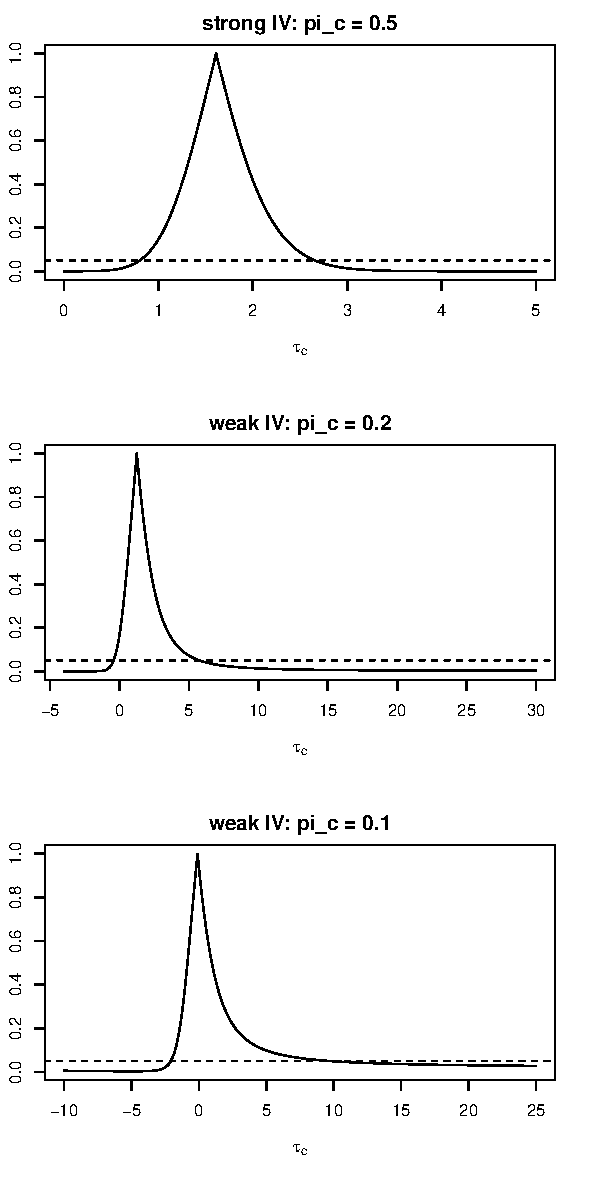
\includegraphics[width=\textwidth]{figures/FARci_simulation1.pdf}
                \caption{第 1 次实现}
                \label{fig::FARci-realization1}
        \end{subfigure}%
\begin{subfigure}[b]{0.45\textwidth}
                \centering
                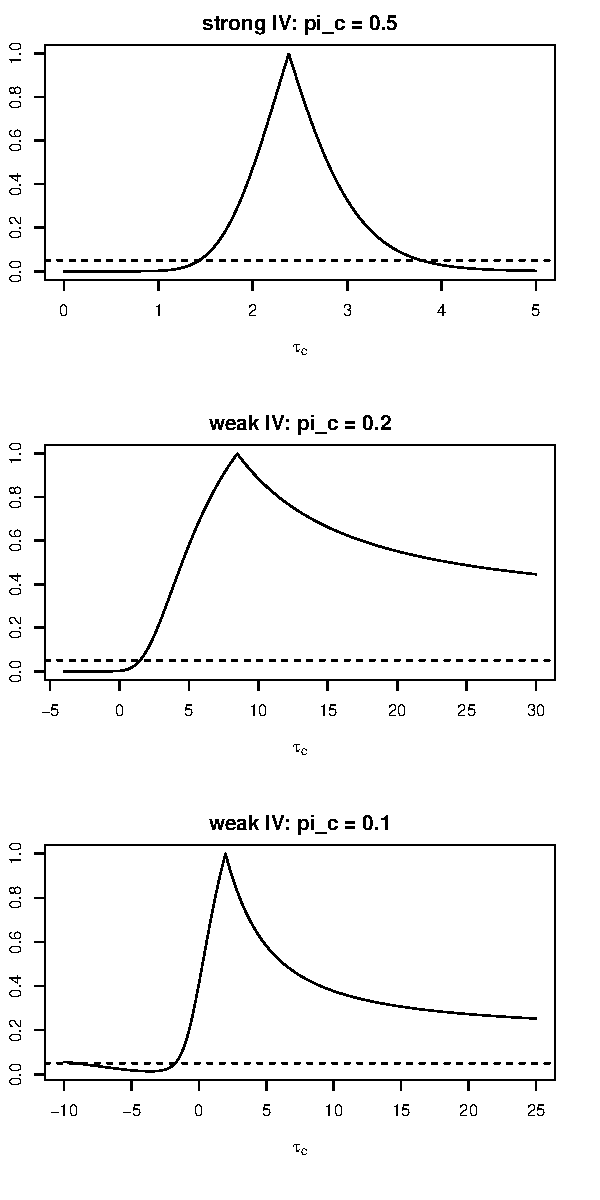
\includegraphics[width=\textwidth]{figures/FARci_simulation2.pdf}
                \caption{第 2 次实现}
                \label{fig::FARci-realization2}
        \end{subfigure}%        
\caption{不同$\pi_\cp$下模拟数据的 FAR 置信区间：两次实现}\label{fg::FAR-ci-simulation}
\end{figure}







\section{实例应用}
\label{sec::cace-application}


\ri{mediation}包中的\ri{jobs}数据集来自求职干预研究 JOBS II，这是一项研究职业培训干预对失业者成效的随机实地实验。\ri{treat}表示参与者是否被随机选入 JOBS II 培训项目，\ri{comply}表示是否实际参加。一个关注的结果是\ri{job_seek}，用于衡量求职自我效能感，取值为 1 至 5。协变量包括\ri{sex}、\ri{age}、\ri{marital}、\ri{nonwhite}、\ri{educ}和\ri{income}。 

 \begin{lstlisting}
> jobsdata = read.csv("jobsdata.csv")
> Z = jobsdata$treat
> D = jobsdata$comply
> Y = jobsdata$job_seek
> getX     = lm(treat ~ sex + age + marital 
+               + nonwhite + educ + income,
+               data = jobsdata)
> X = model.matrix(getX)[, -1]
\end{lstlisting}


可用$\hat{\tau}_\cp$估计$\tau_\cp$，并分别根据$\hat{V}_{\hat{A}}$和自助法计算标准误。还可进行协变量调整，得到$\hat{\tau}_{\cp,\textsc{L}}$，并用自助法估计标准误。结果如下，各方法的点估计与标准误都较稳定。 
 \begin{lstlisting}
> ## without covariates
> res = rbind(IV_Wald_delta(Z, D, Y),
+             IV_Wald_bootstrap(Z, D, Y, n.boot = 10^3))
> ## with covariates 
> res = rbind(res, 
+             IV_Lin_bootstrap(Z, D, Y, X, n.boot = 10^3)) 
> res = cbind(res, res[, 1] - 1.96*res[, 2],
+             res[, 1] + 1.96*res[, 2])
> row.names(res) = c("delta", "bootstrap", "with covariates")
> colnames(res)  = c("est", "se", "lower CI", "upper CI")
> round(res, 3)
                  est    se lower CI upper CI
delta           0.109 0.081   -0.050    0.268
bootstrap       0.109 0.083   -0.054    0.271
with covariates 0.118 0.082   -0.042    0.278
\end{lstlisting}



也可通过反演检验构造 FAR 置信集合，结果与上述置信区间类似。 
 \begin{lstlisting}
                   lower CI upper CI
without covariates   -0.050    0.267
with covariates      -0.047    0.282
\end{lstlisting}

图\ref{fig::FAR-p-value}给出了一系列检验的$p$值。 

\begin{figure}[ht]
\centering
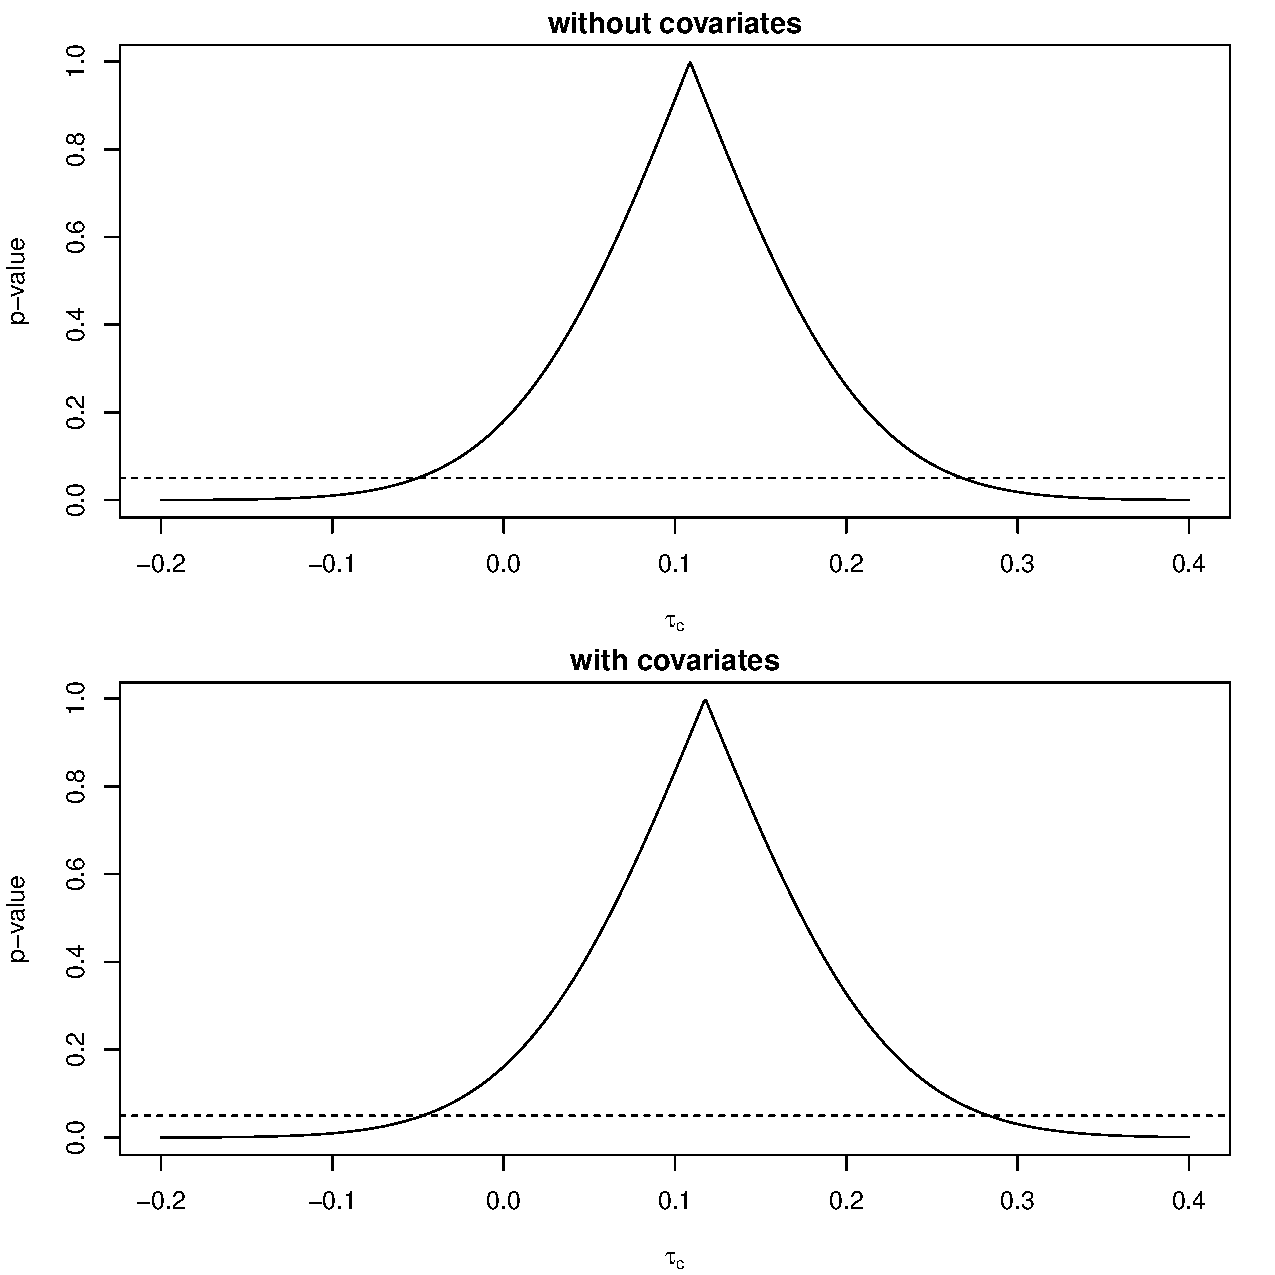
\includegraphics[width = \textwidth]{figures/farci_jobs.pdf}
\caption{通过反演检验构造的$\tau_\cp$置信区间：上图未调整协变量，下图调整了协变量}\label{fig::FAR-p-value}
\end{figure}




\section{CACE 的解释}\label{eq::interpret-iv-double}

潜在结果$\{ D(1), D(0), Y(1), Y(0)  \}$是针对处理分配$Z$这一假想干预定义的，因此$\tau_\cp$是依从者中处理分配对结果的平均因果效应。幸运的是，依从者满足$D=Z$，所以也可以把$\tau_\cp$解释为依从者中实际接受的处理对结果的平均因果效应。这部分回答了科学研究的问题。 

 

一些论文使用不同记号。例如，\citet{angrist1996identification}在一个二乘二析因实验中，用$Y_i(z,d)$表示单位$i$在处理分配为$z$、实际接受处理为$d$时的潜在结果。\footnote{“析因实验”这一名称来自实验设计文献\citep{dasgupta2014causal}，指实验者向每个单位随机分配多个因子，因而处理有多个水平。}\citet[][Section 3.1]{angrist2022empirical}回顾了采用这一记号的学术渊源。在此记号下，排除限制可表述如下。



\begin{assumption}[排除限制]
\label{assume::ER-double-index}
对所有$i$，有$Y_i(z,d) = Y_i(d)$，即潜在结果仅为$d$的函数。
\end{assumption}


由下面的因果图可见，假设\ref{assume::ER-double-index}排除了$Z$到$Y$的直接箭头。在这种情况下，$Z$是$D$的工具变量。 
\begin{center}
$
\xymatrix{
 && & U  \ar[dl] \ar[dr] &\\
Z \ar[rr] &&D \ar[rr]&&Y
}
$
\end{center}
在假设\ref{assume::ER-double-index}下，扩展记号$Y_i(z,d)$简化为$Y_i(d)$，这也解释了“排除限制”的名称。因此，对$d=0,1$有$Y_i(1,d) = Y_i(0,d)$；结合假设\ref{assume::Mono}，可得
\begin{eqnarray*}
Y_i(z=1) - Y_i(z=0) &=& Y_i(1, D_i(1)) - Y_i(0, D_i(0)) \\
&=& \left \{ \begin{array} {ll}
0 , & \text{if} \hspace{2mm}  U_i = \at, \\
0 , & \text{if}  \hspace{2mm}  U_i = \nt,\\
Y_i(d=1) - Y_i(d=0) ,& \text{if} \hspace{2mm} U_i = \cp.
\end{array}
\right.  
\end{eqnarray*}
这里特意区分潜在结果是针对$z$、$d$还是两者定义的，以免混淆。此前对$\tau_Y$的分解仍成立，从而得到\citet{imbens1994identification}和\citet{angrist1996identification}的以下结论。

回顾$D$上的平均因果效应$\tau_D = E\{D(1)  - D(0) \},$，再将$Y$上的平均因果效应定义为$\tau_Y = E\{ Y(D(1)) - Y(D(0))  \}$，将依从者平均因果效应定义为
$$
\tau_\cp =  E\{  Y(d=1) - Y(d=0) \mid U = \cp \}.
$$

\begin{theorem}\label{thm::iv-double-index}
在假设\ref{assume::Mono}至\ref{assume::ER-double-index}下，有
$$
Y(D(1)) - Y(D(0)) = \{  D(1)  - D(0) \} \times \{ Y(d=1) - Y(d=0) \}
$$
以及
$
\tau_\cp   =   \tau_Y /  \tau_D  .
$
\end{theorem}

除记号的相应调整外，证明与定理\ref{thm::CACE-identification}几乎相同，留作习题\ref{para::iv-alternative-form-theorem}。使用记号$Y_i(d)$，更便于将$\tau_\cp$解释为依从者中实际接受处理对结果的平均因果效应。 



 




 
\section{作业习题}



 
\paragraph{Wald 估计量的方差问题}\label{problem::infinite-var-iv}

证明 $\var(\hat{\tau}_\cp) = \infty$。 



\paragraph{Wald 估计量渐近方差及其估计}\label{problem::var-iv-estimate}


考虑$n\rightarrow \infty$的大样本情形。先证明$\sqrt{n}(\hat{\tau}_\cp - \tau_\cp) \rightarrow \textsc{N}(0, V)$依分布收敛，并求出$V$；再证明$\hat{V}_{\hat{A}} /V \rightarrow 1$依概率收敛。 

 
 
 
\paragraph{\citet{imbens1994identification}与\citet{angrist1996identification}的主要定理的证明} 
 \label{para::iv-alternative-form-theorem}
 
 证明定理 \ref{thm::iv-double-index}。 
 


\paragraph{FAR 置信区间的类型判别}\label{para::FAR-CI-cases}

例\ref{eg::FAR-CI-noX}中的置信集合可以是一个闭区间、两个不相连的区间、空集或整条实数轴。分别求出每种情形的确切条件。
 
 
 \paragraph{含协变量 FAR 模拟}\label{para::FAR-CI-simulation-X}

图\ref{fg::FAR-ci-simulation}给出了不使用协变量的 FAR 置信集合。对完全随机实验中调整协变量后的 FAR 置信集合进行类似模拟。 
 
 
\paragraph{序数型处理情形分析}\label{para::iv-ordinal-treatment}

\citet{angrist1995two}讨论了一种更一般的设定：工具变量$Z$为二元变量，实际接受的处理$D \in \{0,1,\ldots, J\}$为有序变量，结果为$Y$。相对于二元工具变量，实际接受处理有潜在取值$D(1)$与$D(0)$；相对于工具变量和实际接受处理的联合干预，结果有潜在取值$Y(z,d)$。将第\ref{eq::interpret-iv-double}节及相应工具变量假设推广如下。

\begin{assumption}\label{assumption::iv-ordinal-treatment}
有以下假设：(1) 随机化，$Z\ind \{   D(z),  Y(z,d)  : z=0,1; d = 0,1,\ldots, J \}$；(2) 单调性，$D(1) \geq D(0)$；(3) 排除限制，对所有$z=0,1$和$ d = 0,1,\ldots, J $均有$Y(z,d) = Y(d)$。 
\end{assumption}

他们证明了下面的定理 \ref{thm::iv-ordinal-treatment}。

\begin{theorem}\label{thm::iv-ordinal-treatment}
在假设\ref{assumption::iv-ordinal-treatment}下，
$$
\frac{  E(Y\mid Z=1) - E(Y\mid Z=0) }{ E(D\mid Z=1) - E(D\mid Z=0)  }
= \sum_{j=1}^J  w_j E\{  Y(j) - Y(j-1)  \mid D(1) \geq j > D(0) \}
$$
其中
$$
w_j = \frac{   \pr\{  D(1) \geq j > D(0)   \}   }{   \sum_{j'=1}^J  \pr\{  D(1) \geq j' > D(0)   \}   }.
$$
\end{theorem}



证明定理 \ref{thm::iv-ordinal-treatment}。

注：$J=1$时，定理\ref{thm::iv-ordinal-treatment}退化为定理\ref{thm::iv-double-index}。对于一般的$J$，标准工具变量公式识别的是若干潜在亚组效应的加权平均。权重与由$  D(1) \geq j > D(0) $定义的潜在亚组的概率成正比，亚组效应$E\{  Y(j) - Y(j-1)  \mid D(1) \geq j > D(0) \}$比较实际接受处理的相邻水平。但这些潜在亚组相互重叠，因此这一加权平均未必容易解释。



证明可能较为繁琐。一个技巧是，将处理分配为$z$时实际接受的处理与结果写为
$$
D(z) = \sum_{j=0}^J j 1\{ D(z) = j\} ,\quad 
Y(D(z)) = \sum_{j=0}^J  Y(j)1\{ D(z) = j\} 
$$
从而得到
$$
D(1) - D(0) = \sum_{j=0}^J j [ 1\{ D(1) = j\} -1\{ D(0) = j\} ]
$$
以及
$$
 Y(D(1))  - Y(D(0))   = 
\sum_{j=0}^J Y(j)   [ 1\{ D(1) = j \}   - 1\{ D(0) = j \}  ].
$$
再对适当选定的序列$(f_j)$与$(g_j)$，应用下面的{\it Abel 引理}，也称{\it 分部求和公式}：
$$
\sum_{j=0}^J  f_j (g_{j+1} - g_j) 
= 
f_J g_{J+1} - f_0 g_0  - \sum_{j=1}^J g_j  (f_j - f_{j-1})
$$ 





 
 


\paragraph{数据分析：流感疫苗接种鼓励设计\citep{mcdonald1992effects}}\label{problem::flushot}
 

\ri{fludata.txt}数据集来自\citet{mcdonald1992effects}的一项随机鼓励设计，\citet{hirano2000assessing}也重新分析过这一数据集。其变量如下：

\begin{tabular}{ll}
\hline 
\texttt{assign} & 是否受到接种流感疫苗鼓励的二元指标\\
\texttt{receive} & 是否实际接种流感疫苗的二元指标 \\
\texttt{outcome} & 是否因流感相关原因住院的二元结果\\
\texttt{age} & 患者年龄\\
\texttt{sex} & 患者性别\\
\texttt{race} & 患者种族\\
\texttt{copd} &  慢性阻塞性肺病\\
\texttt{dm} & 糖尿病\\
\texttt{heartd} & 心脏病\\
\texttt{renal} & 肾病\\
\texttt{liverd} & 肝病\\
\hline 
\end{tabular}


分析随机干预实验数据。 
 


\paragraph{基于协变量的 IV 估计}\label{hw::iv-conditional-x}

在\ri{R}中实现第\ref{section::unconfounded-IV}节提到的估计量及其方差估计量。 

注：本题有助于完成习题\ref{hw::analyze-karolinska-iv}。 



\paragraph{Karolinska 数据再分析}\label{hw::analyze-karolinska-iv}

重新考虑习题\ref{hw::Karolinska-dr}。\citet{rubin2008objective}用 Karolinska 数据说明工具变量方法。在\texttt{karolinska.txt}中，是否在高诊疗量医院确诊，可视为是否在高诊疗量医院接受治疗的工具变量。在给定其他观测协变量后，这一设定是合理的，详见\citet{rubin2008objective}的分析。 


基于观测数据验证工具变量法的有效性。 

 
 
 \paragraph{数据分析：职业培训项目}

文件\texttt{jobtraining.rtf}说明了数据文件\texttt{X.csv}与\texttt{Y.csv}的内容。 

\texttt{X.csv}包含处理前协变量。也可以将抽样权重变量\texttt{wgt}视为一个协变量；许多既有分析都采用了这种简化，尽管它在调查数据分析中始终存在争议。请分别进行调整与不调整协变量的分析。 

\texttt{Y.csv}包含抽样权重、处理分配、实际接受的处理以及许多处理后变量。因此，根据研究问题不同，可以选择多种结果。数据还存在若干复杂之处：一些结果缺失；失业者没有工资；结果还在多个时间点重复观测。分析时，请详细说明研究问题与估计量的选择。 

注：\citet{schochet2008does}分析了原始数据。\citet{frumento2012evaluating}根据后文第\ref{chapter::principal-stratification}章的框架，进行了更复杂的分析。 


 \paragraph{推荐阅读}

\citet{angrist1996identification}将计量经济学中的工具变量视角与基于潜在结果的统计因果推断联系起来，并通过一个应用说明了这一联系的价值。 

工具变量方法的其他早期文献还包括\citet{permutt1989simultaneous}、\citet{sommer1991estimating}、\citet{baker1994paired}和\citet{cuzick1997adjusting}。 


  
    
\chapter{分解混合分布与工具变量不等式}
 \label{chapter::iv-inequalities}

 
 第\ref{chapter::iv-experiment}章中的IV模型需要满足假设\ref{assume::random}至\ref{assume::ER}：
 \begin{enumerate}
 \item
 $Z\ind \{D(1), D(0) ,Y(1), Y(0)   \}$;
 \item
 $\pr(U = \df) = 0$;
 \item 
 对于$U=\at$或$\nt$，有$Y(1) = Y(0)$。 
 \end{enumerate}


表\ref{table::obs-latent}总结了在单调性假设下可观测的组别及其对应的潜在组别。 


\begin{table}[h]
\centering
\caption{假设\ref{assume::Mono}下的可观测组别与潜在组别}\label{table::obs-latent}
\begin{tabular}{cccc}
\hline 
$Z$ & $D$ & $D(1)$ & 潜在组别 \\
\hline 
$Z=1$ & $D=1$ & $D(1) = 1$ & $U = \cp$或$\at$ \\
$Z=1$ & $D=0$ & $D(1) = 0$ & $U = \nt$ \\ 
$Z=0$ & $D=1$ & $D(0) = 1$ & $U = \at$  \\ 
$Z=0$ & $D=0$ & $D(0) = 0$ & $U = \cp$或$\nt$ \\
\hline 
\end{tabular}
\end{table}


有趣的是，假设\ref{assume::random}至\ref{assume::ER}联合起来具有一些可检验的推论。\citet{balke1997bounds}将其称为{\it 工具变量不等式}。本章直观地推导这些不等式的一个特例。只要识别出由$U$定义的各潜在组内的潜在结果均值，即可直接得到证明。 

\section{分解混合分布}
\label{sec::disentangle-mixtures}


我们在下面的定理\ref{thm::cace-mixture-components}中总结了主要结果。
定义
$$
\pi_u = \pr(U = u) \quad  \quad  (u=\at, \nt, \cp) 
$$ 
为类型为$U=u$的个体的比例；同时定义
$$
\mu_{zu} = E\{  Y(z) \mid U = u\}\quad  \quad (z=0,1;u=\at, \nt, \cp) .
$$ 
为类型$U=u$下潜在结果$Y(z) $的均值。
排除限制假设意味着$\mu_{1\nt} = \mu_{0\nt} $且$\mu_{1\at} = \mu_{0\at} $。令$\mu_{\nt}$与$\mu_{\at} $分别表示这两种均值。

\begin{theorem}
\label{thm::cace-mixture-components}
在假设\ref{assume::random}至\ref{assume::ER}下，我们可以通过以下方式确定各类潜在类型的比例：
\begin{eqnarray*}
 \pi_\nt &=& \pr(D=0\mid Z=1)  ,\\
  \pi_\at &=&\pr(D=1\mid Z=0) , \\
  \pi_\cp &=& E(D\mid Z=1) - E(D\mid Z=0) ,
\end{eqnarray*}
同时可以确定各类型下潜在结果的均值：
\begin{eqnarray*}
  \mu_{\nt} &=& E(Y\mid Z=1, D=0) ,\\
 \mu_{\at} &=& E(Y\mid Z=0, D=1),\\
 \mu_{1\cp} &=& \pi_\cp^{-1}\left\{   E(DY\mid Z=1 )  -  E(DY\mid Z=0)    \right\}, \\
  \mu_{0\cp}  &=& \pi_\cp^{-1} \big[   E\{ (1-D)Y\mid Z=0 \}  -  E\{(1-D)Y\mid Z=1 \}    \big]. 
\end{eqnarray*}
\end{theorem}
 
 
\begin{myproof}{定理}{\ref{thm::cace-mixture-components}}
第一部分：我们首先确定各类潜在顺从类型的比例。
 never-takers类型的比例可通过下式计算：
\begin{eqnarray*}
\pr(D=0\mid Z=1) 
%&=& \pr\{ D(1) = 0\mid Z=1 \} = \pr\{ D(1) = 0, D(0) = 0 \mid Z=1 \} \\
&=& \pr(U=\nt \mid Z=1)  \\
&=& \pr(U=\nt) \\
&=&  \pi_\nt ,
\end{eqnarray*}
Always-takers类型的比例则为：
\begin{eqnarray*}
\pr(D=1\mid Z=0) 
%&=& \pr\{  D(0) = 1\mid Z=0 \} =  \pr\{ D(1)=1,  D(0) = 1\mid Z=0 \} \\
&=& \pr(U=\at \mid Z=0)  \\
&=& \pr(U=\at) =  \pi_\at . 
\end{eqnarray*}
因此，Compliers类型的比例即为：
\begin{eqnarray*}
\pi_\cp &=& \pr(U=\cp) \\
&=& 1-  \pi_\nt -  \pi_\at  \\
&=& 1 - \pr(D=0\mid Z=1)  - \pr(D=1\mid Z=0) \\
%&=&\pr(D=1\mid Z=1)  - \pr(D=1\mid Z=0) 
&=& E(D\mid Z=1) - E(D\mid Z=0) \\
&=& \tau_D,
\end{eqnarray*}
该结果与之前的讨论一致。尽管我们无法得知每个个体的潜在类型，但我们能够确定各类别的比例。 


第二部分：接下来识别各潜在依从类型内的潜在结果均值。 
%Under Assumption \ref{assume::ER}, 
%$$
%\mu_{1\at} = \mu_{0\at} \equiv \mu_{\at},\quad \mu_{1\nt} = \mu_{0\nt} \equiv \mu_{\nt} .
%$$
观测组$(Z=1,D=0)$仅包含从不接受者，因此$$
E(Y\mid Z=1, D=0) = E\{  Y(1) \mid Z=1, U=\nt \} = E\{  Y(1) \mid   U=\nt \}  =
\mu_{\nt}  . 
$$观测组$(Z=0,D=1)$仅包含始终接受者，因此$$
E(Y\mid Z=0, D=1) = E\{  Y(0) \mid Z=0, U=\at \} = E\{  Y(0) \mid   U=\at \}  =
\mu_{\at} . 
$$观测组$(Z=1,D=1)$既包含依从者，也包含始终接受者，因此\begin{eqnarray*}
E(Y\mid Z=1, D=1) &=& E\{ Y(1)\mid Z=1, D(1)=1\} \\
&=& E\{ Y(1)\mid D(1)=1\}  \\   
&=& \pr\{  D(0)=1 \mid D(1)=1 \} E\{ Y(1)\mid D(1)=1, D(0)=1\}  \\
&&+ \pr\{  D(0)=0 \mid D(1)=1 \}E\{ Y(1)\mid D(1)=1, D(0)=0\}   \\
&=& \frac{\pi_\cp}{\pi_\cp + \pi_\at} \mu_{1\cp} +  \frac{\pi_\at}{\pi_\cp + \pi_\at} \mu_{\at}.
\end{eqnarray*}求解上述线性方程得到\begin{eqnarray*}
\mu_{1\cp} &=& \pi_\cp^{-1} \left\{  (\pi_\cp + \pi_\at)  E(Y\mid Z=1, D=1)  - \pi_\at    E(Y\mid Z=0, D=1)    \right\} \\
&=& \pi_\cp^{-1} \left\{  \pr(D=1\mid Z=1)  E(Y\mid Z=1, D=1) \right.\\
&&\left. \qquad  -\pr(D=1\mid Z=0) E(Y\mid Z=0, D=1)    \right\} \\
&=&  \pi_\cp^{-1}\left\{   E(DY\mid Z=1 )  -  E(DY\mid Z=0)    \right\}.
\end{eqnarray*}观测组$(Z=0,D=0)$既包含依从者，也包含从不接受者，因此\begin{eqnarray*}
E(Y\mid Z=0,D=0) &=& E\{ Y(0)\mid Z=0, D(0)=0\} \\
&=& E\{ Y(0)\mid D(0)=0\} \\ 
&=& \pr\{  D(1)=1 \mid D(0)=0 \} E\{ Y(0)\mid D(1)=1, D(0)=0\}  \\
&&+ \pr\{  D(1)=0 \mid D(0)= 0\}E\{ Y(0)\mid D(1)=0, D(0)=0\}   \\
&=& \frac{\pi_\cp}{\pi_\cp + \pi_\nt} \mu_{0\cp} +  \frac{\pi_\nt}{\pi_\cp + \pi_\nt} \mu_{\nt}.
\end{eqnarray*}求解上述线性方程得到\begin{eqnarray*}
\mu_{0\cp}  &=& \pi_\cp^{-1} \left\{  (\pi_\cp + \pi_\nt)  E(Y\mid Z=0, D=0)  - \pi_\nt    E(Y\mid Z=1, D=0)    \right\} \\
&=& \pi_\cp^{-1} \left\{ \pr(D=0\mid Z=0)  E(Y\mid Z=0, D=0)  \right.\\
&&\left. \qquad  -\pr(D=0\mid Z=1)   E(Y\mid Z=1, D=0)    \right\} \\
&=& \pi_\cp^{-1} \big[   E\{ (1-D)Y\mid Z=0 \}  -  E\{(1-D)Y\mid Z=1 \}    \big]. 
\end{eqnarray*}
\end{myproof}

根据定理\ref{thm::cace-mixture-components}中$\mu_{1\cp} $和$\mu_{0\cp} $的公式，可以将$\tau_\cp = \mu_{1\cp}  - \mu_{0\cp}  $简化为$$
\tau_\cp =  \{  E(Y\mid Z=1) - E(Y\mid Z=0) \}/\pi_\cp ,
$$与此前定理\ref{thm::CACE-identification}的公式一致。 

定理\ref{thm::cace-mixture-components}的核心目标是确定各类潜在结果均值$\mu_{zu} $。\citet{imbens1997estimating}推导出了更为通用的潜在结果分布识别公式；具体细节由习题\ref{hw::disentangle-mixture-distrubution}阐述。



\section{可检验推论：工具变量不等式}


通过定理\ref{thm::cace-mixture-components}绕道推导$\tau_\cp$的公式，还有额外价值吗？有。对于二元结果，以下不等式必然成立：$$
0\leq \mu_{1\cp} \leq 1, \quad 
0\leq \mu_{0\cp} \leq 1, 
$$进而得到四个不等式\begin{eqnarray*}
E(DY\mid Z=1 )  -  E(DY\mid Z=0) &\geq & 0 ,\\
E(DY\mid Z=1 )  -  E(DY\mid Z=0) &\leq  & E(D\mid Z=1) - E(D\mid Z=0)  ,\\ 
E\{ (1-D)Y\mid Z=0 \}  -  E\{(1-D)Y\mid Z=1 \}   &\geq & 0,\\
E\{ (1-D)Y\mid Z=0 \}  -  E\{(1-D)Y\mid Z=1 \}  &\leq & E(D\mid Z=1) - E(D\mid Z=0) . 
\end{eqnarray*}移项后可得到以下统一形式的不等式。


\begin{theorem}[工具变量不等式]\label{thm::iv-inequality}
当结果变量$Y$为二元变量时，假设\ref{assume::random}至\ref{assume::ER}意味着：
\begin{eqnarray}\label{eq::iv-inequalities}
E(Q\mid Z=1) - E(Q\mid Z=0) \geq 0,  
\end{eqnarray}
其中$Q = DY, D(1-Y), (D - 1)Y$以及$D+Y-DY$。
\end{theorem}


在IV假设\ref{assume::random}至\ref{assume::ER}下，$Q = DY, D(1-Y), (D - 1)Y$及$D+Y-DY$的均值差均必须非负。值得注意的是，上述推论仅涉及观测变量的分布特性。任何违反IV不等式的观测结果都会引发对IV假设本身的质疑。 


\citet{balke1997bounds}推导出了含或不含单调性假设时的广义IV不等式；本证明思路源自\citet{jiang2020measurement}提出的针对稍复杂情境的推导方法。定理\ref{thm::iv-inequality}仅针对二元结果变量展开了讨论；习题\ref{hw::ivineq-binary}提供了等价形式，习题\ref{hw::ivineq-general-Y}则给出了适用于一般结果变量的结论。



\section{实例分析}\label{section::binary-y-ivineq}


对于二元结果变量，我们可以利用矩估计法估算所有参数。


\begin{lstlisting}
IVbinary = function(n111, n110, n101, n100, 
                    n011, n010, n001, n000){
  
  n_tr = n111 + n110 + n101 + n100
  n_co = n011 + n010 + n001 + n000
  n    = n_tr + n_co
  
  ## proportions of the latent strata
  pi_n = (n101 + n100)/n_tr
  pi_a = (n011 + n010)/n_co
  pi_c = 1 - pi_n - pi_a
  
  ## four observed means of the outcomes (Z=z,D=d)
  mean_y_11 = n111/(n111 + n110)
  mean_y_10 = n101/(n101 + n100)
  mean_y_01 = n011/(n011 + n010)
  mean_y_00 = n001/(n001 + n000)
  
  ## means of the outcomes of two strata
  mu_n1 = mean_y_10
  mu_a0 = mean_y_01
  ## ER implies the following two means
  mu_n0 = mu_n1
  mu_a1 = mu_a0
  ## stratum (Z=1,D=1) is a mixture of c and a
  mu_c1 = ((pi_c + pi_a)*mean_y_11 - pi_a*mu_a1)/pi_c
  ## stratum (Z=0,D=0) is a mixture of c and n
  mu_c0 = ((pi_c + pi_n)*mean_y_00 - pi_n*mu_n0)/pi_c
  
  ## identifiable quantities from the observed data
  list(pi_c = pi_c, 
       pi_n = pi_n, 
       pi_a = pi_a, 
       mu_c1= mu_c1,
       mu_c0= mu_c0,
       mu_n1= mu_n1,
       mu_n0= mu_n0,
       mu_a1= mu_a1,
       mu_a0= mu_a0,
       tau_c= mu_c1 - mu_c0)
}
\end{lstlisting}


下面我们重新分析两个经典的二元数据实例。 

\begin{example}\label{eg::1-iv-inequalities}
\citet{improve2014endovascular}评估了对临床诊断为主动脉瘤破裂的患者实施急诊腔内修复或开放手术修复策略的效果。患者被随机分配至两种策略之一，主要结果为30天后的生存状态。令$Z$表示分配的处理，其中$Z=1$表示腔内修复策略，$Z=0$表示开放修复策略；令$D$表示实际接受的处理。令$Y$表示生存状态，$Y=1$表示死亡，$Y=0$表示存活。表\ref{tab::data1}汇总了观测数据。
%The estimate of $\tau_\cp $ is $0.131$ with 95\% confidence interval $(-0.036, 0.298)$ including $0$.
使用上述\ri{IVbinary}函数，可得到以下估计结果：
\begin{lstlisting}
> investigators_analysis = IVbinary(n111 = 107,
+                                   n110 = 42,
+                                   n101 = 68,
+                                   n100 = 42,
+                                   n011 = 24,
+                                   n010 = 8,
+                                   n001 = 131,
+                                   n000 = 79)
>                         
> investigators_analysis
$pi_c
[1] 0.4430582

$pi_n
[1] 0.4247104

$pi_a
[1] 0.1322314

$mu_c1
[1] 0.7086064

$mu_c0
[1] 0.6292042

$mu_n1
[1] 0.6181818

$mu_n0
[1] 0.6181818

$mu_a1
[1] 0.75

$mu_a0
[1] 0.75

$tau_c
[1] 0.07940223
\end{lstlisting}
没有证据表明工具变量假设被违反。 
\end{example}


\begin{example}\label{eg::2-iv-inequalities}
在\citet{hirano2000assessing}的研究中，医生被随机选中接收一封鼓励其为流感高风险患者接种疫苗的信。处理为实际接种流感疫苗，结果为是否因流感相关问题到医院就诊的指示变量。然而，一些患者并不依从分配。令$Z_i$为鼓励接种的指示变量：医生收到鼓励信时$Z=1$，否则$Z=0$。令$D$为实际接受的处理。令$Y$为结果：冬季因流感相关原因住院时$Y=0$，否则$Y=1$。数据的更多细节见习题\ref{problem::flushot}，观测数据汇总于表\ref{tab::data2}。
%The estimate of $\tau_\cp $ is $0.116$ with 95\% confidence interval $(-0.061, 0.293)$ including $0$.
使用上述\ri{IVbinary}函数，可得到以下估计结果：
\begin{lstlisting}
> flu_analysis = IVbinary(n111 = 31,
+                         n110 = 422,
+                         n101 = 84,
+                         n100 = 935,
+                         n011 = 30,
+                         n010 = 233,
+                         n001 = 99,
+                         n000 = 1027)
> flu_analysis
$pi_c
[1] 0.1183997

$pi_n
[1] 0.6922554

$pi_a
[1] 0.1893449

$mu_c1
[1] -0.004548064

$mu_c0
[1] 0.1200094

$mu_n1
[1] 0.08243376

$mu_n0
[1] 0.08243376

$mu_a1
[1] 0.1140684

$mu_a0
[1] 0.1140684

$tau_c
[1] -0.1245575
\end{lstlisting}
由于$\hat\mu_{1\cp} < 0$，表明IV假设可能被违反。 
\end{example} 




 \begin{table}[t]
\caption{二元数据与IV不等式}
\begin{center}
\begin{subtable}{0.5\textwidth}
\caption{ \citet{improve2014endovascular}研究数据}
\begin{tabular}{cccccc} 
\hline 
      &   \multicolumn{2}{c}{$Z=1$}  &  &  \multicolumn{2}{c}{$Z=0$}  \\  \cline{2-3} \cline{5-6} 
      & $D=1$  &  $D=0$           &       &  $D=1$  &  $D=0$\\
 $Y=1$ &   107    &      68         &      &    24       &    131        \\
 $Y=0$ &   42    &     42            &      &     8         &     79           \\  
 \hline
\end{tabular}
\label{tab::data1}
\end{subtable}% 
\vspace{0.1in}
\begin{subtable}{0.5\textwidth}
\caption{ \citet{hirano2000assessing}研究数据}
\begin{tabular}{cccccc}
\hline 
      &   \multicolumn{2}{c}{$Z=1$}  &  &  \multicolumn{2}{c}{$Z=0$}  \\  \cline{2-3} \cline{5-6} 
      & $D=1$  &  $D=0$           &       &  $D=1$  &  $D=0$\\
 $Y=1$ &   31    &     85         &      &     30       &    99       \\
 $Y=0$ &   424   &     944            &      &     237         &    1041           \\  
 \hline
\end{tabular}
\label{tab::data2}
\end{subtable}
\end{center}
\end{table}%

 
 
\section{作业习题}

\paragraph{更细致的数据分析}\label{hw::more-data-binary}

实例\ref{eg::1-iv-inequalities}与\ref{eg::2-iv-inequalities}均未涉及估计值的不确定性。请尝试为真实参数计算相应的置信区间。 
 



\paragraph{Compliers群体的风险比}\label{hw::rr-compliers}


对于二元结果变量，可定义Compliers群体的风险比为：
$$
\textsc{rr}_\cp = \frac{  \pr\{  Y(1) = 1\mid U = \cp \}  }{ \pr\{  Y(0) = 1\mid U = \cp \}   } .
$$

试证明：在假设\ref{assume::random}至\ref{assume::ER}下，该值可表示为：
$$
\textsc{rr}_\cp =  \frac{  E(DY\mid Z=1)  - E(DY\mid Z=0)  }{  E\{  (D-1)Y\mid Z=1 \}   - E\{ (D-1)Y\mid Z=0 \} }.
$$



提示：依据定理\ref{thm::cace-mixture-components}，可求得任何$E\{  Y(1) \mid U = \cp \} $与$E\{  Y(0) \mid U = \cp \} $间的对比值。 


\paragraph{分解混合分布：分布层面的结果}\label{hw::disentangle-mixture-distrubution}


本习题是对定理\ref{thm::cace-mixture-components}的拓展。定义
$$
f_{zu}(y) = \pr\{  Y(z) = y  \mid U=u \},  \quad  (z=0,1;u=\at, \nt, \cp)
$$
为潜在类型$U=u$下结果变量$Y(z)$的概率密度函数；同时令
$$
g_{zd}(y) = \pr(Y = y\mid Z=z, D=d)
$$
为观测组$(Z=z, D=d)$中结果变量的条件密度。排除限制假设促使$f_{1\nt}(y) = f_{0\nt} (y) $且$f_{1\at}(y) = f_{0\at}(y) $，令$f_{\nt}(y)$与$ f_{\at} (y) $分别为这两种分布。 



请证明定理\ref{thm::cace-mixture-components-distribution}的内容。  


 
\begin{theorem}
\label{thm::cace-mixture-components-distribution}
在假设\ref{assume::random}至\ref{assume::ER}之下，各类潜在类型下的结果变量概率密度可由下式确定：
\begin{eqnarray*}
  f_{\nt}(y) &=& g_{10}(y) ,\\
  f_{\at} (y) &=& g_{01}(y),\\
f_{1\cp}(y) &=& \pi_\cp^{-1} \{   \pr(D=1\mid Z=1 )g_{11}(y)  -  \pr(D=1\mid Z=0) g_{01}(y)   \} , \\
f_{0\cp} (y) &=& \pi_\cp^{-1} \{  \pr(D=0\mid Z=0)  g_{00}(y)  -  \pr(D=0\mid Z=1)  g_{10}(y)    \} . 
\end{eqnarray*}
\end{theorem}



 





\paragraph{定理\ref{thm::iv-inequality}的等价表达}
\label{hw::ivineq-binary}

\eqref{eq::iv-inequalities}中的不等式可改写为\begin{eqnarray*}
\pr(D=1, Y=y\mid Z=1) &\geq & \pr(D=1, Y=y\mid Z=0), \\
\pr(D=0, Y=y\mid Z=0) &\geq & \pr(D=0, Y=y\mid Z=1)
\end{eqnarray*}对$y=0,1$均成立。 



\paragraph{一般结果变量的IV不等式}
\label{hw::ivineq-general-Y}

对于一般型结果变量$Y$，试证明假设\ref{assume::random}至\ref{assume::ER}能推导出：
\begin{eqnarray*}
\pr(D=1, Y\geq y\mid Z=1) &\geq & \pr(D=1, Y\geq y\mid Z=0), \\
\pr(D=1, Y <  y\mid Z=1) &\geq & \pr(D=1, Y <  y\mid Z=0), \\
\pr(D=0, Y\geq y\mid Z=0) &\geq & \pr(D=0, Y\geq y\mid Z=1),\\
\pr(D=0, Y <  y\mid Z=0) &\geq & \pr(D=0, Y <  y\mid Z=1)
\end{eqnarray*}
对所有$y$值均成立。 
 
提示：\citet{imbens1997estimating}与\citet{kitagawa2015test}探讨了类似结论。可借助Kolmogorov-Smirnov统计量构建检验形式：
$$
\text{KS}_1 = \max_{y} \Big |
\frac{  \sumn Z_i D_i  1(Y_i \leq y)  }{ \sumn Z_i D_i  } - \frac{  \sumn (1-Z_i) D_i  1(Y_i \leq y)  }{ \sumn (1-Z_i) D_i  }
\Big |.
$$



\paragraph{IV不等式的实例演示}

请分别给出满足全部IV不等式以及不满足全部IV不等式的两个实例。需具体描述二元变量$(Z,D,Y)$的联合分布特征。 

 
 
 \paragraph{关键假设的违背情形}\label{eq::violations-of-IV}

定理\ref{thm::CACE-identification}的成立依赖于随机化、单调性与排除限制三个假设，后两者在随机实验中也无法直接检验。当这些假设被违背时，IV估计法同样无法得到正确的CACE估计值。习题要求论证以下两种违背情形，对应\citet{angrist1996identification}的两个命题。记$\pi_u = \pr(U=u)$且$\tau_u = E\{  Y(1) - Y(0) \mid U=u \}$（$u=\at, \nt, \cp, \df$）。 


\begin{theorem}
\label{theorem::wald-violation-assumptions}
(a) 在假设\ref{assume::random}和\ref{assume::Mono}成立、而不要求排除限制时，有$$
\frac{ E(Y\mid Z=1) - E(Y\mid Z=0) }{ E(D\mid Z=1) - E(D \mid Z=0) } - \tau_\cp 
= \frac{  \pi_\at \tau_\at + \pi_\nt \tau_\nt  }{  \pi_\cp } .
$$
 

(b) 在假设\ref{assume::random}和\ref{assume::ER}成立、而不要求单调性时，有$$
\frac{ E(Y\mid Z=1) - E(Y\mid Z=0) }{ E(D\mid Z=1) - E(D \mid Z=0) } - \tau_\cp 
= \frac{  \pi_\df (\tau_\cp + \tau_\df )  }{   \pi_\cp - \pi_\df   }.
$$
\end{theorem}
 
请证明定理\ref{theorem::wald-violation-assumptions}的内容。 

 
 \paragraph{其他分析方法的局限}\label{problem::as-treated-analysis}

第\ref{sec::disentangle-mixtures}节推导工具变量不等式时，通过识别各潜在层的比例及其潜在结果的条件均值，解开了混合分布。这些结果有助于理解其他看似合理的分析方法的缺陷。下面回顾三种估计量，并假设\ref{assume::random}至\ref{assume::ER}成立。   


\begin{enumerate}
\item 
{\it 按实际治疗分析}比较实际接受处理和对照的单位的结果均值，得到$$
\tau_\textsc{at} = E(Y\mid D=1) - E(Y\mid D=0).
$$证明$$
\tau_\textsc{at} = \frac{  \pi_\at \mu_\at + \pr(Z=1)\pi_\cp \mu_{1\cp}   }{   \pr(D=1) } 
- \frac{  \pi_\nt \mu_\nt + \pr(Z=0) \pi_\cp \mu_{0\cp}   }{   \pr(D=0) } .
$$


\item 
{\it 符合方案分析}比较处理组和对照组中依从所分配处理的单位，得到$$
\tau_\textsc{pp} = E(Y\mid Z=1, D=1) - E(Y\mid Z=0, D=0).
$$证明$$
\tau_\textsc{pp} =\frac{  \pi_\at \mu_\at + \pi_\cp \mu_{1\cp} }{  \pi_\at   + \pi_\cp }
- \frac{  \pi_\nt \mu_\nt + \pi_\cp \mu_{0\cp} }{  \pi_\nt   + \pi_\cp }.
$$


\item 
亦可考察实际接受干预与未接受干预组之间的条件均值差，即
\begin{eqnarray*}
\tau_{Z=1} &=& E(Y\mid Z=1, D=1) - E(Y\mid Z=1, D=0),\\ 
\tau_{Z=0} &=& E(Y\mid Z=0, D=1) - E(Y\mid Z=0, D=0).
\end{eqnarray*}
试证明：
$$
\tau_{Z=1}  = \frac{  \pi_\at \mu_\at + \pi_\cp \mu_{1\cp} }{  \pi_\at   + \pi_\cp } - \mu_\nt,\quad
\tau_{Z=0} = \mu_\at - \frac{  \pi_\nt \mu_\nt + \pi_\cp \mu_{0\cp} }{  \pi_\nt   + \pi_\cp }.
$$
\end{enumerate}
 
 
\paragraph{总体平均因果效应的界限}\label{para::bounds-ACE}


使用第\ref{eq::interpret-iv-double}节的记号，推广第\ref{sec::disentangle-mixtures}节的讨论。以潜在结果$Y(d)$定义实际接受的处理对结果的平均因果效应为$$
\delta = E\{  Y(d=1) - Y(d=0) \},
$$由于记号变化，将$\mu_{zu} $的定义相应改为$$
m_{du} = E\{  Y(d) \mid U = u\},\quad  (z=0,1;u=\at, \nt, \cp) 
$$它们满足$$
\delta = \sum_{u = \at, \nt, \cp}  \pi_u  (m_{1u} - m_{0u}).
$$

第\ref{sec::disentangle-mixtures}节已确定$\pi_\at$、$\pi_\nt$、$\pi_\cp$、$m_{1\at} = \mu_{1 \at}$、$m_{0\nt} = \mu_{0\nt }$、$m_{1\cp} = \mu_{1\cp}$及$m_{0\cp} = \mu_{0\cp}$的值，但$m_{0 \at}$与$m_{1\nt }$未知，因此无法直接测定$\delta$。若结果变量有界，则可界定$\delta$的取值区间。  

\begin{theorem}
\label{thm::bound-on-ACE}
在假设\ref{assume::Mono}至\ref{assume::ER-double-index}成立、且结果有界于$[\underline{y}, \overline{y}]$时，有$\underline{\delta} \leq  \delta  \leq \overline{\delta}$，其中$$
\underline{\delta} =  \delta'  - \overline{y} \pr(D=1\mid Z=0) + \underline{y} \pr(D=0\mid Z=1)
$$和$$
\overline{\delta} = \delta'  -   \underline{y} \pr(D=1\mid Z=0) +  \overline{y}  \pr(D=0\mid Z=1) 
$$并记$\delta' = E(DY\mid Z=1) - E(Y-DY\mid Z=0) .$
\end{theorem}

试证明定理\ref{thm::bound-on-ACE}的内容。 
 
 
说明：在结果为二元变量的特殊情形下，这些界限简化为$$
\underline{\delta} =   E(DY\mid Z=1) - E( D+Y-DY\mid Z=0)  
$$和$$
\overline{\delta} =  E(DY+1-D\mid Z=1) - E(Y-DY\mid Z=0) .
 $$
 
 
 \paragraph{单侧不遵从现象与统计推断}\label{para::15-onesidednoncompliance}
 
考虑一种随机激励实验：对照组个体不可取得干预措施。记个体$i$的干预分配变量为$Z_i$，实际干预接受状况为$D_i$，观测结果为$Y_i$。所谓单侧不遵从现象，即满足：
$$
Z_i=0 \Longrightarrow  D_i = 0 \quad (i=1,\ldots, n). 
$$
假定假设\ref{assume::random}成立。 
 
 
\begin{enumerate}
[(1)]
\item 
在该情境下，单调性假设\ref{assume::Mono}是否成立？该情境下由$\{ D_i(1), D_i(0)  \}$可定义的潜在类型共有几种？怎样通过观测数据测定其占比？  

\item 
请具体表述排除限制假设内容。在该假设下，证明$E\{  Y(z) \mid U = u \}$可由观测数据确定。给出所有可能的$z$与$u$值对应的公式。在此情境下如何测定CACE？  

 

\item
如果观测到所有单位$i$的处理前协变量$X_i$，如何利用协变量信息提高CACE的估计效率？  
 
 
 \item 
 在假设\ref{assume::random}下，排除限制假设\ref{assume::ER}具有可检验的推论，即单侧不依从情形的工具变量不等式。写出这些不等式。
 
\item
\citet{sommer1991estimating}报告了如下数据集： 
 
 \begin{center}
\begin{tabular}{cccccc} 
\hline 
      &   \multicolumn{2}{c}{$Z=1$}  &  &  \multicolumn{2}{c}{$Z=0$}  \\  \cline{2-3} \cline{5-6} 
      & $D=1$  &  $D=0$           &       &  $D=1$  &  $D=0$\\
 $Y=1$ &   9663    &     2385         &      &     0       &    11514       \\
 $Y=0$ &   12   &     34            &      &     0         &    74           \\  
 \hline 
\end{tabular}
 \end{center}
 
此实验中$Z$为是否分配维生素A补充剂的指示变量，$D$为实际接受补充剂的状况，$Y$为存活与否的指示变量。该试验在印度尼西亚实施。请重新分析该数据。 
 \end{enumerate}
 
 
说明：\citet{bloom1984accounting}最早讨论单侧不依从，并提出估计量$\hat\tau_\cp = \hat\tau_Y / \hat\tau_D$，有时称为Bloom估计量。\citet{bloom1984accounting}的记号与本章不同。 

 
 
 
 
  \paragraph{单侧不遵从与部分遵从现象}
\label{para::one-sided-partial-adherence}
 
\citet[][Table 3]{sanders2021incorporating}报告了以下随机对照试验数据，该试验旨在估计针对精神病性障碍患者的戒烟干预效果。 

\begin{center}
\begin{tabular}{cccc}
\hline  
分配组别& 实际接受的处理 &组别人数& \# 阳性结果人数 \\
\hline  
对照 & 无& 151 &25 \\
处理& 无& 35 & 7 \\
处理& 部分& 42& 17 \\
处理& 全部& 70& 40\\
\hline 
\end{tabular}
\end{center}

实际接受的处理分为三级：“完全”指参加全部$8$次治疗，“部分”指参加$5$至$7$次，“无”指参加$<5$次。结果是在三个月时测量的二元指标，表示吸烟量是否相对基线减少至少$50\%$。


本题中，处理分配$Z$为二元变量，而实际接受的处理$D$取$0, 0.5, 1$三个值，分别对应“无”“部分”和“完全”。三级$D$使问题更复杂，但被分配到对照组时它只能为0。此时有多少个潜在层$U = \{ D(1), D(0) \} $？能否识别它们的比例？

如何将排除限制推广到本题？可以关注哪些因果效应？能否识别这些效应？ 

根据上述问题分析数据。 



  

 \paragraph{推荐阅读}

\citet{balke1997bounds}推导了更一般的工具变量不等式。 

   
     
\chapter{工具变量的计量经济学视角}
 \label{chapter::iv-econometric}
 
 
第\ref{chapter::iv-experiment}章与第\ref{chapter::iv-inequalities}章从实验角度探讨了工具变量法。图\ref{fig::causal-diagram-IV}则直观展示了这一方法的理论依据。 
 
 
\begin{figure}[h]
\centering 
$
\xymatrix{
 && & U  \ar[dl] \ar[dr] &\\
Z \ar[rr] &&D \ar[rr]&&Y
}
$
\caption{工具变量的因果图}\label{fig::causal-diagram-IV}
\end{figure} 
 
 
 
在存在不依从的鼓励设计中，$Z$经过随机化，因此与实际接受处理$D$和结果$Y$之间的混杂变量$U$独立。处理分配$Z$对结果$Y$没有直接效应，而只经由实际接受处理$D$影响结果$Y$，因而充当$D$的工具变量。这里的工具变量由实验者产生。 


许多应用无法随机化。若处理$D$与结果$Y$之间存在未测量混杂，应如何作因果推断？计量经济学的一个巧妙想法是寻找{\it 自然实验}，模拟鼓励设计。为识别$D$对$Y$的因果效应，可寻找另一个变量$Z$，使其满足图\ref{fig::causal-diagram-IV}编码的假设。变量$Z$必须满足以下条件：
\begin{enumerate}
\item
近似具备随机化特性，从而与未观测混淆因素$U$独立；
\item
能够改变治疗干预$D$的分布规律；
\item
它只能通过$D$间接影响结果$Y$，不能直接影响结果。
\end{enumerate}
若上述条件均被满足，则$Z$便可作为估计$D$对$Y$影响程度的有效工具变量。 



本章介绍基于线性回归的传统计量经济学工具变量视角。\citet{imbens1994identification}与\citet{angrist1996identification}澄清了这一视角与第\ref{chapter::iv-experiment}、\ref{chapter::iv-inequalities}章实验视角之间的联系，是一项基础性贡献。下面先看例子，再讨论代数细节。 



\section{工具变量法的实证研究案例}
 
 
 
寻找合适的工具变量与其说是科学，不如说是一门艺术。尽管后文涉及的代数运算在统计学中并不算复杂，但如何在实证研究中精准找到符合要求工具变量却极具挑战性。以下列举若干典型实例。  


\begin{example} 
鼓励设计中，$Z$是随机分配的处理，$D$是最终接受的处理，$Y$是结果。如第\ref{chapter::iv-experiment}章所述，图\ref{fig::causal-diagram-IV}的工具变量假设在双盲随机对照试验中较为合理，这是工具变量的理想情形。 
\end{example}


 
 
 \begin{example}
 \citet{hearst1986delayed}发现越战征兵抽签中号码较小的男性随后死亡率较高；其解释为兵役产生的负面影响。\citet{angrist1990lifetime}补充指出这类男性后期收入也偏低，同样可归结为兵役所致。由于抽签号码属随机生成、号码较小者恰更可能服兵役，且该号码对死亡率与收入并无直接影响，故图\ref{fig::causal-diagram-IV}条件完全成立。\citet{angrist1996identification}正是以此为基础重新分析了实验数据：其中抽签号码为工具变量、兵役为处理干预、死亡率或收入则为观测结果。 
\end{example}




\begin{example}
\citet{angrist1991does}以出生季度作为工具变量，测算了受教育年限对收入的贡献值。出生季度具有近似随机化特征：一方面美国多数州规定儿童满六周岁方可入学；另一方面义务教育法要求最低入学年龄为十六周岁。此外出生季度亦不直接影响收入值。 
\end{example}


\begin{example}
\citet{angrist1998children}选用兄弟姐妹性别构成作为工具变量，研究了家庭规模对母亲劳动参与的影响。同理，此变量亦具备近似随机化特征：同性别双胞胎会显著提升第三胎仍为同性别的概率，且该变量同样不直接决定母亲的就业行为。 
\end{example}


\begin{example}\label{example::Card1993}
\citet{card1993using}研究教育对工资的影响，以居住地点距大学远近的地理差异作为工具变量。具体而言，$Z$包含是否在两年制或四年制大学附近长大的虚拟变量。尽管该研究很经典，它未必是一个理想的工具变量例子：父母选择住址可能并非随机，而且成长地点本身也可能影响后来工资。 
\end{example}



\begin{example}
\citet{voight2012plasma}用{\it 孟德尔随机化}研究血浆高密度脂蛋白（HDL）胆固醇对心肌梗死风险的因果效应。他们采用某些单核苷酸多态性（SNP）作为 HDL 的遗传工具变量：依据孟德尔第二定律，它们与 HDL 和心肌梗死之间的未测量混杂独立，且仅通过 HDL 影响心肌梗死。孟德尔随机化的更多细节见第\ref{chapter::iv-mr}章。 
\end{example}



\section{普通最小二乘法简述}



在引入工具变量法前，我们先简要回顾普通最小二乘法（见\ref{appendix::basic-linear-regression}章）。该方法是统计学经典内容，但其数学定义形式各异，且不同形式间的选择将影响理论解释。 

第一种视角基于投影。给定具有有限二阶矩的随机变量$Y$与随机变量或向量$D$，定义总体 OLS 系数
\begin{eqnarray*}
\beta  &=& \arg\min_b E(Y - D  \tran b  )^2 \\
&=& E(DD\tran)^{-1} E(DY),
\end{eqnarray*}
再定义总体残差$\varepsilon = Y -  D  \tran \beta $。根据定义，$Y$可分解为
\begin{eqnarray}\label{eq::olsdecomposition}
Y = D  \tran \beta  + \varepsilon,
\end{eqnarray}
且必满足
$$
E(  D \varepsilon) = 0.
$$
根据数据$(D_i,Y_i)_{i=1}^n \iidsim (D, Y)$，$\beta$的 OLS 估计是矩估计量
$$
\hat{\beta} = \left(  \sumn D_i D_i\tran \right)^{-1}   \sumn D_i Y_i  . 
$$
由于
\begin{eqnarray*}
\hat{\beta}  &=& \left(  \sumn D_i D_i\tran \right)^{-1}  \sumn D_i ( D_i\tran \beta + \varepsilon_i   )  \\
&=& \beta + \left(  \sumn D_i D_i\tran \right)^{-1} \sumn D_i  \varepsilon_i   ,
\end{eqnarray*}
利用大数定律和$E(\varepsilon D) = 0.$，可证明$\hat{\beta}$一致估计$\beta$。$\cov(\hat\beta)$的经典 EHW 稳健方差估计为
$$
\hat{V}_\textsc{ehw} = \left(  \sumn D_i D_i\tran \right)^{-1}
\left(  \sumn \hat{\varepsilon}_i^2 D_i D_i\tran \right)
\left(  \sumn D_i D_i\tran \right)^{-1}
$$
其中$\hat{\varepsilon}_i  = Y_i - D_i\tran \hat{\beta}$是残差。 




第二种视角把
\begin{eqnarray}\label{eq::ols-true-model}
Y = D  \tran \beta  + \varepsilon,
\end{eqnarray}
视为数据生成过程的真实模型：给定随机变量$(D, \varepsilon)$，根据线性方程\eqref{eq::ols-true-model}生成$Y$。在这一生成过程中，$\varepsilon$与$D$可能相关，即$E( D \varepsilon) \neq  0$，图\ref{fig::endogenous-regressor}就是例子。这与第一种视角有根本区别：第一种视角中的$E(\varepsilon D) = 0$由总体 OLS 的定义自动保证。因此，当样本量$n$趋于无穷时，OLS 估计量可能不一致：
$$
\hat{\beta} \rightarrow \beta + E(DD\tran)^{-1} E(D\varepsilon) \neq \beta 
$$
这里为依概率收敛。 


本节最后根据\eqref{eq::ols-true-model}定义{\it 内生}与{\it 外生}回归变量，不过这些术语在计量经济学中并非只有一种定义。 



\begin{definition}
\label{def::endogenous-exogenous}
当$E(\varepsilon D) \neq  0$时，回归变量$D$称为{\it 内生的}；当$E(\varepsilon D) =  0$时，回归变量$D$称为{\it 外生的}。 
\end{definition}

定义\ref{def::endogenous-exogenous}采用计量经济学的标准术语。$E(\varepsilon D) \neq  0$时，也称存在{\it 内生性}；$E(\varepsilon D) =  0$时，也称满足{\it 外生性}。

在第一种最小二乘视角下，由于$E(\varepsilon D) =  0$为定义前提，内生与外生的区分毫无意义。持此观点的统计学家常觉这两概念难以理解，进而难以接受工具变量的必要性。若要深入理解工具变量法，必须转而采用第二种视角。 




 

\begin{figure}[h]
\centering
\begin{subfigure}[]{0.4\textwidth}
                \centering
$
\xymatrix{
& U \ar[dl] \ar[dr]& \\
D \ar[dr] & & \varepsilon \ar[dl] \\
&Y&
}
$                \caption{$E(D\varepsilon) \neq 0$}
        \end{subfigure}%
        
        \begin{subfigure}[]{0.4\textwidth}
                \centering
$
\xymatrix{
&\varepsilon  \ar[dl] \ar[dr] &\\
D \ar[rr]&&Y
}
$
                \caption{对$\varepsilon$边际化处理}
        \end{subfigure}%
        
\caption{内生变量$D$的不同表现形式。上图中$U$代表$D$与$\varepsilon$共享的未观测混淆因素。}\label{fig::endogenous-regressor}
\end{figure}



\section{线性工具变量模型}
\label{sec::linear-iv-model}



$D$内生时，OLS 估计不一致，必须利用额外信息才能构造$\beta$的一致估计量。下面关注如下线性工具变量模型：


\begin{definition}
[线性工具变量模型]\label{def::linear-iv-model}
定义观测模型为
$$
Y = D  \tran \beta  + \varepsilon ,
$$
且须满足
\begin{eqnarray}\label{eq::iv-moment-condition}
E(\varepsilon Z) = 0 . 
\end{eqnarray}
\end{definition}


定义\ref{def::linear-iv-model}的线性工具变量模型可用下列因果图表示： 
%\begin{figure}[h]
%\centering 
$$
\xymatrix{
&&&\varepsilon  \ar[dl] \ar[dr] &\\
Z\ar[rr]&&D \ar[rr]&&Y
}
$$
%\caption{Instrumental variable}
%\end{figure}

上述模型虽然允许$E(\varepsilon D) \neq 0$，却提出了额外矩条件\eqref{eq::iv-moment-condition}。通过加入截距项使$E(\varepsilon) = 0$后，此条件可解读为$Z$与误差项$\varepsilon$不相关。但任何随机噪声均与$\varepsilon$不相关，故必须补充条件确保$Z$对估计$\beta$切实有效。直观而言，该条件要求$Z$须与$D$存在相关性——具体技术细节下文详述。  
 

数学条件\eqref{eq::iv-moment-condition}看似简单，但实证研究的一项核心挑战，正是找到满足\eqref{eq::iv-moment-condition}的变量$Z$。条件\eqref{eq::iv-moment-condition}涉及不可观测的$\varepsilon$，因此一般无法检验。 
 


\section{恰好识别情形}
\label{sec::iv-just-identify}

我们先探讨$Z$与$D$维度相同且$E(ZD\tran)$满秩的特殊情形。此时条件$E(\varepsilon Z) = 0$等价于
$$
E\{  Z (Y -  D \tran \beta) \} = 0 .
$$
解此线性系统可得
$$
E(  ZY)  = E(ZD\tran) \beta  \\
 \Longrightarrow 
\beta = E(ZD\tran) ^{-1} E(  ZY)  
$$
前提是$E(ZD\tran)$非退化矩阵。当$E(\varepsilon D) = 0$时，即$D$本身充当工具变量，此式即退化为普通最小二乘估计量：
\begin{eqnarray}\label{eq::iv-estimator}
\hat{\beta}_\textsc{iv} = \left(  \sumn Z_i D_i\tran \right)^{-1}  \sumn Z_iY_i.
\end{eqnarray}

将$D$与$Z$都为标量的情形具体推导出来有助于理解，见下面的例\ref{eg::scalar-iv}。

\begin{example}\label{eg::scalar-iv}
在含截距、$D$与$Z$均为标量的简单情形中，模型为
$$
\left\{ \begin{array}{l}
Y = \alpha +  \beta  D + \varepsilon ,\\
E(\varepsilon) = 0, \quad \cov(\varepsilon, Z) = 0,
\end{array}
\right.
$$
由该模型，
$$
\cov( Z, Y ) = \beta \cov(Z, D) 
$$
因而
$$
 \beta = \frac{ \cov( Z, Y )   }{ \cov(Z, D) }.
$$
将分子分母同时除以$\var(Z)$，得到
$$
\beta =  \frac{ \cov( Z, Y ) / \var(Z)  }{ \cov(Z, D) / \var(Z) },
$$
即$Y$和$D$分别对$Z$作 OLS 回归所得$Z$系数之比。若$Z$为二元变量，这两个系数就是均值差（见习题\ref{problem::pols-binary}），$\beta$简化为
$$
\beta = \frac{ E(Y\mid Z=1) - E(Y\mid Z=0)  }{ E(D\mid Z=1) - E(D\mid Z=0) } .
$$
与定理\ref{thm::CACE-identification}的识别公式相同。也就是说，对于二元工具变量$Z$和二元处理$D$，工具变量估计在潜在结果框架下恢复 CACE。这是\citet{imbens1994identification}与\citet{angrist1996identification}的关键结论。  
\end{example}



 

\section{过度识别情形}
\label{sec::sec::iv-over-identify}

第\ref{sec::iv-just-identify}节讨论的是{\it 恰好识别}情形。若$Z$的维数小于$D$，且$E(ZD\tran)$不满列秩，则方程$E(  ZY)  = E(ZD\tran) \beta$有无穷多个解。这就是{\it 欠识别}：即使有$Z$，也无法唯一确定系数$\beta$。这一困难问题超出本书范围。为保证可识别性，工具变量数至少应与内生回归变量数一样多。 

若$Z$的维数大于$D$，且$E(ZD\tran)$满列秩，就有多种办法根据$E(  ZY)  = E(ZD\tran) \beta$确定$\beta$。而且，样本对应方程
$$
n^{-1} \sumn Z_iY_i = n^{-1} \sumn Z_i D_i\tran \beta
$$
的方程数多于未知参数数，可能没有精确解。 


处理过度识别的一种巧妙计算方法是{\it 两阶段最小二乘}（TSLS）估计量\citep{theil1953estimation, basmann1957generalized}，它分两步进行。

\begin{definition}
[两阶段最小二乘法]\label{def::2sls}
以$Z$为工具变量的$D$系数的 TSLS 估计量定义如下。 
\begin{enumerate}
\item
将$D$对$Z$作 OLS 回归，得到拟合值$\hat{D}_i\ (i=1,\ldots, n)$。若$D_i$为向量，则逐分量回归以获得$\hat{D}_i$。将拟合向量按行$\hat{D}_i\tran $组成矩阵$\hat{D}$；
\item
以$\hat{D}$为自变量回归$Y$，所得斜率系数即为$\hat{\beta}_\textsc{tsls}$值。  
\end{enumerate}
\end{definition}
 

为说明 TSLS 为什么有效，需要进一步的代数推导。将其明确写为
\begin{eqnarray} 
\hat{\beta}_\textsc{tsls} &=& \left(  \sumn \hat{D}_i\hat{D}_i\tran \right) ^{-1} 
\sumn \hat{D}_i Y_i  \label{eq::2sls-definition} \\
&=& \left(  \sumn \hat{D}_i\hat{D}_i\tran \right) ^{-1} 
\sumn \hat{D}_i (D_i \tran \beta + \varepsilon_i)  \nonumber  \\
&=& \left(  \sumn \hat{D}_i\hat{D}_i\tran \right) ^{-1} 
\sumn \hat{D}_i D_i \tran \beta + \left(  \sumn \hat{D}_i\hat{D}_i\tran \right) ^{-1} \sumn \hat{D}_i  \varepsilon_i .   \nonumber 
\end{eqnarray}
第一阶段 OLS 保证$D_i  = \hat{D}_i + \check D_i$，且拟合值与残差正交，即
\begin{equation} \label{eq::ols-orthogonal}
\sumn \hat{D}_i  \check D_i\tran = 0
\end{equation}
是与$D_i$维数相同的零方阵。正交关系\eqref{eq::ols-orthogonal}蕴含
$$
\sumn \hat{D}_i D_i \tran = \sumn \hat{D}_i\hat{D}_i\tran,
$$
从而
\begin{eqnarray}
\label{eq::2sls-ols}
\hat{\beta}_\textsc{tsls} = \beta + \left(  \sumn \hat{D}_i\hat{D}_i\tran \right) ^{-1} \sumn \hat{D}_i  \varepsilon_i.
\end{eqnarray}
第一阶段 OLS 还保证
\begin{equation}
\label{eq::ols-donz}
\hat{D}_i = \hat{\Gamma}\tran  Z_i 
\end{equation}
进而
\begin{eqnarray}
\label{eq::2sls-consistency}
\hat{\beta}_\textsc{tsls} = \beta + \left\{  \hat{\Gamma}\tran  \left(  n^{-1}  \sumn Z_i Z_i\tran  \right) \hat{\Gamma}  \right\}  ^{-1}  
\hat{\Gamma}\tran  \left( n^{-1} \sumn Z_i  \varepsilon_i \right) . 
\end{eqnarray}
由\eqref{eq::2sls-consistency}，利用大数定律以及$n^{-1} \sumn Z_i  \varepsilon_i $的概率极限为$E(Z\varepsilon) = 0$，即可得到 TSLS 的一致性。还可利用\eqref{eq::2sls-consistency}证明：$Z$与$D$维数相同时，$\hat{\beta}_\textsc{tsls} $与第\ref{sec::iv-just-identify}节定义的$\hat{\beta}_\textsc{iv} $在数值上相同，见习题\ref{prob::algebra-tsls}。 




根据\eqref{eq::2sls-ols}，标准误可按以下方式计算：先求残差$\hat{\varepsilon}_i = Y_i - \hat{\beta}_\textsc{tsls}\tran D_i$，再计算稳健方差估计
$$
\hat{V}_\textsc{tsls} = \left( \sumn  \hat{D}_i \hat{D}_i\tran  \right)^{-1}
 \left( \sumn \hat{\varepsilon}_i ^2  \hat{D}_i \hat{D}_i\tran  \right)
\left( \sumn  \hat{D}_i \hat{D}_i\tran  \right)^{-1} . 
$$
各$\hat{\varepsilon}_i$不是第二阶段 OLS 的残差$  Y_i - \hat{\beta}_\textsc{tsls}\tran \hat{D}_i $，因此$\hat{V}_\textsc{tsls} $不同于直接从第二阶段 OLS 得到的稳健方差估计。 




\section{特殊应用案例：单工具变量与单内生处理}


本节关注一个应用广泛的简单情形：单个工具变量与单个内生处理。考虑{\it 结构方程}
\begin{eqnarray}
\label{eq::strucrual-iv}
\left\{
\begin{array}{l}
Y_i = \beta_0 + \beta_1 D_i + \beta_2\tran X_i + \varepsilon_{i},\\
D_i = \gamma_0 + \gamma_1 Z_i + \gamma_2 \tran X_i + \varepsilon_{2i},
\end{array}
\right.
\end{eqnarray}
其中$D_i$是表示目标处理的标量内生回归变量，即$E(\varepsilon_{i} D_i) \neq 0$；$Z_i$是$D_i$的标量工具变量，即$E(\varepsilon_{i} Z_i) = 0$；$X_i$包含其他外生回归变量，即$E(\varepsilon_{i} X_i) = 0$。这是将$D$替换为$(1, D, X)$、$Z$替换为$(1, Z, X)$的特例。 



\subsection{两阶段最小二乘实现}

定义\ref{def::2sls}中的 TSLS 估计量简化如下。 

\begin{definition}
[在此情境下TSLS简化为两步操作：]\label{def::tsls-single}
根据\eqref{eq::strucrual-iv}，TSLS 分为以下两步。
\begin{enumerate}
\item
将$D$对$(1, Z,X)$作 OLS 回归，得到拟合值$\hat{D}_i\ (i=1,\ldots, n)$，组成向量$\hat{D}$； 

\item 
将$Y$对$(1, \hat{D}, X)$作 OLS 回归，得到系数$\hat{\beta}_\textsc{tsls}$，特别是$\hat{D}$的系数$\hat{\beta}_{1,\textsc{tsls}}$。 
\end{enumerate}
\end{definition}



\subsection{间接最小二乘法}


结构方程\eqref{eq::strucrual-iv}蕴含
\begin{eqnarray*}
Y_i &=&\beta_0 + \beta_1 (\gamma_0 + \gamma_1 Z_i + \gamma_2 \tran X_i + \varepsilon_{2i}) + \beta_2\tran X_i + \varepsilon_{i} \\
&=& (\beta_0 + \beta_1\gamma_0 ) + \beta_1  \gamma_1 Z_i  + ( \beta_2 + \beta_1 \gamma_2 )\tran X_i  + ( \varepsilon_{i} + \beta_1 \varepsilon_{2i} ).
\end{eqnarray*}
定义$\Gamma_0 = \beta_0 + \beta_1\gamma_0, \Gamma_1  =  \beta_1  \gamma_1, \Gamma_2 = \beta_2 + \beta_1 \gamma_2$与$\varepsilon_{1i} = \varepsilon_{i} + \beta_1 \varepsilon_{2i}$，则得到方程
\begin{eqnarray}
\label{eq::reduced-iv}
\left\{
\begin{array}{l}
Y_i =\Gamma_0 + \Gamma_1 Z_i + \Gamma_2\tran X_i + \varepsilon_{1i},\\
D_i = \gamma_0 + \gamma_1 Z_i + \gamma_2 \tran X_i + \varepsilon_{2i},
\end{array}
\right.
\end{eqnarray}
这称为{\it 简约式}，与\eqref{eq::strucrual-iv}的{\it 结构式}相对应。目标参数等于两个系数之比
$$
\beta_1 = \Gamma_1 / \gamma_1.
$$
简约式左边为因变量$Y$与$D$，右边为外生变量$Z$与$X$，满足
$$
E( Z \varepsilon_{1i} ) = E( Z \varepsilon_{2i} )  = 0, \quad 
E( X \varepsilon_{1i} ) = E( X \varepsilon_{2i} )  = 0.
$$
更重要的是，OLS 一致估计简约式\eqref{eq::reduced-iv}的系数。 


简约式\eqref{eq::reduced-iv}表明，两个 OLS 系数$\hat{\Gamma}_1$与$\hat{\gamma}_1$的比值是$\beta_1$的合理估计。这称为{\it 间接最小二乘}（ILS）估计量：
$$
\hat{\beta}_{1,\textsc{ils}} =  \hat{\Gamma}_1 / \hat{\gamma}_1 .
$$
有意思的是，在\eqref{eq::strucrual-iv}下，它与 TSLS 估计量数值相同。

\begin{theorem}
\label{thm::ils=2sls}
%Under \eqref{eq::strucrual-iv}, we have  
在\eqref{eq::strucrual-iv}只有一个内生处理和一个工具变量时，
$$
\hat{\beta}_{1,\textsc{ils}}   = \hat{\beta}_{1,\textsc{tsls}} . 
$$
\end{theorem}

定理\ref{thm::ils=2sls}是一个代数事实。\citet[][Section A.3]{imbens2014instrumental}指出了它，但未给出证明，证明留作习题\ref{para::tsls-ils}。比值公式也清楚说明，当工具变量较弱、即$\gamma_1 $接近零时，TSLS 估计的有限样本性质较差。 



\subsection{弱工具变量问题}

下面的方法更简单、透明，对弱工具变量也更稳健，但计算量较大。简约式\eqref{eq::reduced-iv}还意味着，对任意$b$，
\begin{eqnarray}
\label{eq::anderson-rubin-reg}
Y_i  - bD_i = (\Gamma_0 -b \gamma_0 ) +  (\Gamma_1  - b \gamma_1 ) Z_i
+ (\Gamma_2 - b \gamma_2  ) \tran X_i  + ( \varepsilon_{1i} -  b \varepsilon_{2i} )
\end{eqnarray}
在真实值$b = \beta_1$处，$Z_i$的系数必为$0$。据此，可反演$H_0(b): \beta_1 = b$的检验，构造$\beta_1$的置信集合：
$$
\left\{ b:  | t_Z(b) | \leq z_{1-\alpha/2} \right\},
$$
其中$t_Z(b) $是采用 EHW 标准误拟合\eqref{eq::anderson-rubin-reg}时$Z$系数的$t$统计量，$z_{1-\alpha/2}$是标准正态分布的$1-\alpha/2$分位数。与基于 TSLS 的 Wald 型区间相比，这个集合更稳健，类似第\ref{chapter::iv-experiment}章的 FAR 置信集合。使用此方法甚至不必先计算 TSLS 估计。若仅需在\eqref{eq::strucrual-iv}下检验$\beta_1 = 0$，只需根据简约式将$Y$作 OLS 回归即可。 



\section{实证分析示例}\label{sec::tsls-application}

 

重新考察例\ref{example::Card1993}。\citet{card1993using}用青年男性全国纵向调查估计教育对收入的因果效应，数据包含 1966 年年龄 14—24 岁的 3010 名男性。\citet{card1993using}以成长地点距大学远近的地理差异作为教育的工具变量。$Z$表示是否在四年制大学附近长大，$D$为受教育年限，结果$Y$是 1976 年对数工资，范围为 4.6—7.8。其他协变量包括种族、年龄、年龄平方、家庭居住结构分类以及过去居住地区。原文的家庭结构类别列举重复出现“与双亲同住”，另列“仅与母亲同住”。 



\begin{lstlisting}
> library("car")
> ## Card Data
> card.data = read.csv("card1995.csv")
> Y = card.data[, "lwage"]
> D = card.data[, "educ"]
> Z = card.data[, "nearc4"]
> X = card.data[, c("exper", "expersq", "black", "south", 
+                   "smsa", "reg661", "reg662", "reg663", 
+                   "reg664", "reg665", "reg666", 
+                   "reg667", "reg668", "smsa66")]
> X = as.matrix(X)
\end{lstlisting}


基于 TSLS，可得下面的点估计与$95\%$置信区间。 
\begin{lstlisting}
> Dhat    = lm(D ~ Z + X)$fitted.values
> tslsreg = lm(Y ~ Dhat + X)
> tslsest = coef(tslsreg)[2]
> ## correct se by changing the residuals
> res.correct       = Y - cbind(1, D, X)%*%coef(tslsreg)
> tslsreg$residuals = as.vector(res.correct)
> tslsse = sqrt(hccm(tslsreg, type = "hc0")[2, 2])
> res = c(tslsest, tslsest - 1.96*tslsse, tslsest + 1.96*tslsse)
> names(res) = c("TSLS", "lower CI", "upper CI")
> round(res, 3)
    TSLS lower CI upper CI 
   0.132    0.026    0.237 
\end{lstlisting}


采用 FAR 置信集合策略，可计算随$b$变化的$p$值。 
\begin{lstlisting}
> BetaAR   = seq(-0.1, 0.4, 0.001)
> PvalueAR = sapply(BetaAR, function(b){
+   Y_b   = Y - b*D
+   ARreg = lm(Y_b ~ Z + X)
+   coefZ = coef(ARreg)[2]
+   seZ   = sqrt(hccm(ARreg)[2, 2])
+   Tstat = coefZ/seZ
+   (1 - pnorm(abs(Tstat)))*2
+ })
\end{lstlisting}
图\ref{fig::card-far-ci}给出了针对$D$系数的一系列检验的$p$值，使用以下\ri{R}代码：
\begin{lstlisting}
> plot(PvalueAR ~ BetaAR, type = "l",
+      xlab = "coefficient of D",
+      ylab = "p-value",
+      main = "Fieller-Anderson-Rubin interval based on Card's data")
> point.est = BetaAR[which.max(PvalueAR)]
> abline(h = 0.05, lty = 2, col = "grey")
> abline(v = point.est, lty = 2, col = "grey")
> ARCI = range(BetaAR[PvalueAR >= 0.05])
> abline(v = ARCI[1], lty = 2, col = "grey")
> abline(v = ARCI[2], lty = 2, col = "grey")
\end{lstlisting}
以使$p$值最大的$b$作为点估计，并以$p$值大于 0.05 的$b$取值区域作为置信区间。 
\begin{lstlisting}
> FARres = c(point.est, ARCI)
> names(FARres) = c("FAR est", "lower CI", "upper CI")
> round(FARres, 3)
 FAR est lower CI upper CI 
   0.132    0.028    0.282
\end{lstlisting}
比较 TSLS 与 FAR 方法，两者置信下限很接近，上限略有不同，可能源于 TSLS 估计量分布的右尾较重。总体上，由于本例的工具变量不弱，两种方法结果相似。 
 


\begin{figure}
\centering 
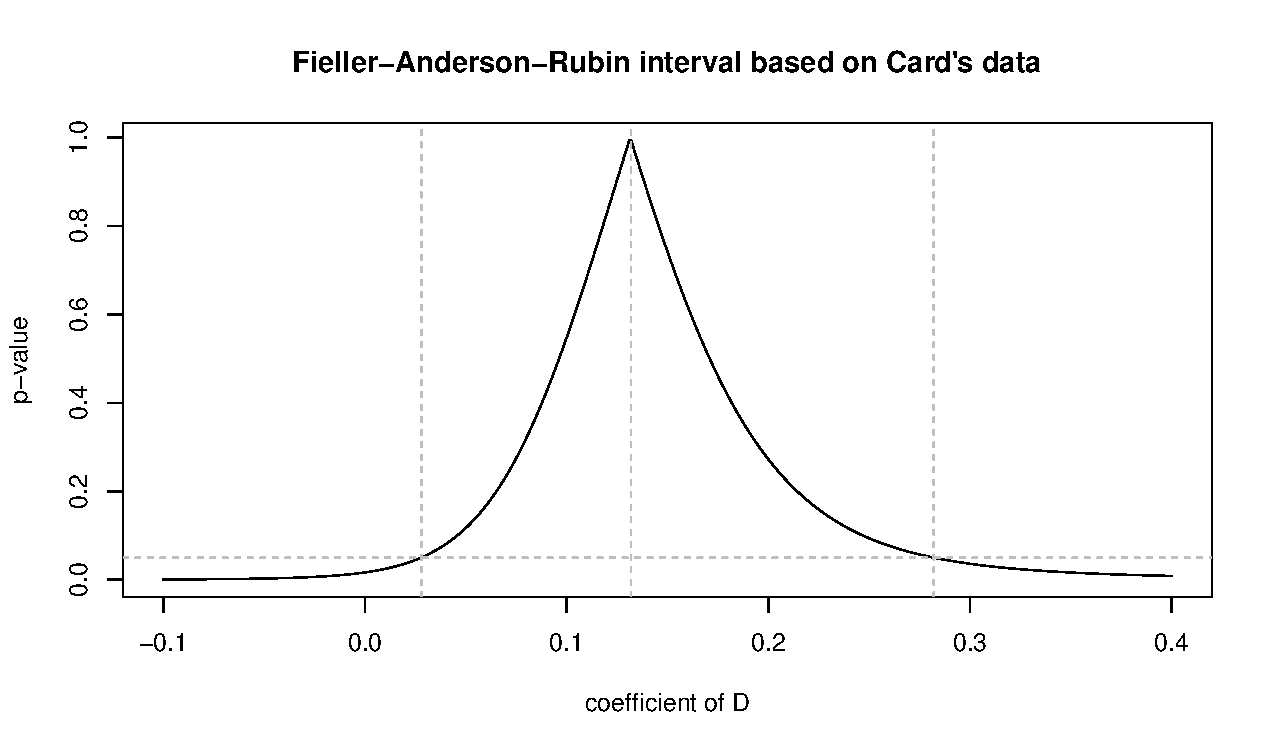
\includegraphics[width = \textwidth]{figures/FAR_Carddata.pdf}
\caption{通过反演检验重新分析\citet{card1993using}的数据} \label{fig::card-far-ci} 
\end{figure}

 
 
 
\section{习题作业}

\paragraph{第\ref{sec::sec::iv-over-identify}节 TSLS 的进一步代数推导}\label{prob::algebra-tsls}

\begin{enumerate}
\item 
证明\eqref{eq::ols-donz}中的$\hat \Gamma$等于
$$
\hat{\Gamma} = \left(  \sumn Z_i Z_i\tran  \right)^{-1} \sumn Z_i D_i\tran .
$$

\item
证明：若$Z$与$D$维数相同，且
$$
n^{-1} \sumn Z_i Z_i\tran, \quad n^{-1} \sumn Z_i D_i\tran
$$
均可逆，则\eqref{eq::2sls-definition}定义的$\hat{\beta}_\textsc{tsls} $退化为\eqref{eq::iv-estimator}定义的$ \hat{\beta}_\textsc{iv}$。 
\end{enumerate}

\paragraph{间接法等价性证明}\label{para::tsls-ils}
证明定理 \ref{thm::ils=2sls}。 


注：使用第\ref{appendix::basic-linear-regression}章的 FWL 定理。 



\paragraph{线性工具变量模型中的控制函数}\label{para::control-function-iv}

下面的定义 \ref{def::cf} 与上面的定义 \ref{def::2sls} 相对应。

\begin{definition}
[探讨第三种估计思路的适用性。]\label{def::cf}
将控制函数估计量$\hat{\beta}_\textsc{cf}$定义如下。
\begin{enumerate}
\item
将$D$对$Z$作 OLS 回归，得到残差$\check D_i\ (i=1,\ldots, n)$。若$D_i$为向量，则逐分量回归，得到$\check D_i$。将残差向量按行$\check{D}_i\tran $组成矩阵$\check{D}$；
\item
将$Y$对$D$和$\check{D}$作 OLS 回归，取$D$的系数为$\hat{\beta}_\textsc{cf}$。  
\end{enumerate}
\end{definition}
 
 证明 $\hat{\beta}_\textsc{cf} = \hat{\beta}_\textsc{tsls}$。
 
 
 注：可利用习题\ref{hw::ols-orthogonal}与\ref{hw::ols-transform-regressors}证明。在定义\ref{def::cf}中，第一步得到的$\check{D}$称为第二步的控制函数。\citet{hausman1978specification}指出了这一结果，\citet{wooldridge2015control}则更一般地讨论了复杂模型中的控制函数方法。 
 
  


 

%\paragraph{Data analysis: \citet{card1993using}}
%
%\citet{card1993using} used the geographic variation in college proximity to estimate the return to schooling. The treatment is education and the outcome is log wage. The IV is the college proximity. 
%\texttt{card.csv} is a slightly modified version of the data from Card's homepage with detailed explanations of the variable names in \texttt{code\_bk.txt}.
%
%You can dichotomize the education variable and infer the LATE. How do you choose the threshold for the dichotomization? Are the results sensitive to your choice? Conduct an analysis with covariates. 
%
%Without dichotomizing the education variable, you can use the standard two-stage least squares estimator. Compare the results to the above analysis.
%
%What if the return of education is nonlinear? Do the data provide information for us to test the nonlinearity?
%


\paragraph{数据分析：\citet{efron1991compliance}}

\citet{efron1991compliance}是较早用潜在结果框架处理不依从的研究之一。原始随机实验“脂质研究诊所冠心病一级预防试验”（LRC-CPPT）旨在评价考来烯胺对胆固醇水平的效应。\texttt{EF.csv}数据第一列为处理／对照二元指标，第二列为实际服用量占名义剂量的比例，最后三列为胆固醇水平。受试者不知道自己被分到药物还是安慰剂，但副作用差异可能使依从行为随分组而不同。所有人被指定相同名义剂量，并服用相同时间。第 3 列$C_3$测于告知低胆固醇饮食益处之前；第 4 列$C_4,$测于饮食建议之后、药物或安慰剂随机分配之前；第 5 列$C_5$为随机分配后胆固醇读数的均值，每两个月测量一次，受试者的随访时间平均为 7.3 年。\citet{efron1991compliance}以胆固醇变化$C_5 - 0.25C_3 - 0.75C_4$为最终结果，原论文有更详细说明。 
 

这里的数据结构比第\ref{chapter::iv-experiment}、\ref{chapter::iv-inequalities}章的不依从问题更复杂。\citet{jin2008principal}基于后文第\ref{chapter::principal-stratification}章的思想重新分析了数据。可按自己对问题的理解选择分析方法，但需说明选择依据。本题没有公认的标准答案。 




 \paragraph{推荐阅读}


\citet{imbens2014instrumental}介绍了计量经济学家的工具变量视角。 

        
     
\chapter{工具变量方法的应用：模糊回归不连续设计}
 \label{chapter::iv-frdd}



第\ref{chapter::overlap}章介绍的回归不连续设计以及第\ref{chapter::iv-experiment}章至第\ref{chapter::iv-econometric}章介绍的工具变量方法，都是{\it 自然实验}的两个重要范例。这些研究设计与第\ref{part::rcts}章所述的随机对照实验相比虽不够理想，却具备类似随机实验的特征；正因如此它们才被称为自然实验。 


将回归不连续设计与工具变量方法相结合便形成了{\it 模糊回归不连续设计}，这也是一种重要的自然实验形式。本文将先通过实例引入该概念，随后给出其数学表述。  




\section{实例说明}
\label{sec::frdd-motivation}

第\ref{chapter::overlap}章已介绍过回归不连续设计。以下三个实例与其略有区别：在这些实例中，实验处理并非由运行变量直接决定；相反，运行变量会在断点处使个体接受处理的概率发生突变。 

\begin{example}\label{eg::indianroad}
2000年，印度政府启动了“总理乡村道路计划”；至2015年，该计划已为近20万个村庄修建了全天候道路。\citet{asher2020rural}基于村庄级数据，运用回归不连续设计来估算新修道路对各种经济指标的影响。该计划的实施标准参照了2001年人口普查数据，以特定阈值来决定优先资助的村庄规模。若某村庄在统计年份前新建了道路，则视为接受了处理。不过，村庄人口规模与阈值间的差距并不决定处理状态本身，仅在断点0处影响到接受处理的概率。 
\end{example}


\begin{example}\label{eg::italianuniversity}
\citet{li2015evaluating}借助2004至2006年间两所意大利大学新生的数据，评估了助学金对辍学率的因果效应。凡家庭标准化收入低于15,000欧元的申请者均有资格获得资助。为简化分析，我们定义运行变量为15,000减去标准化家庭收入。由于必须先提交申请方能获得资助，因此资格判定与申请行为共同决定了最终处理状态。尽管运行变量同样在断点0处改变了处理概率，但它本身亦不决定处理状态。 
\end{example}



\begin{example}
\citet{amarante2016cash}估计了胎儿在子宫内暴露于一项社会援助计划对出生结局的影响。他们利用乌拉圭{\it Plan de Atención Nacional a la Emergencia Social}计划形成的断点回归。这是一项面向最贫困的百分之十家庭的临时社会援助计划，于2005年4月至2007年12月实施。预测收入评分低于预定阈值的家庭被分配参加该计划。这一评分并不完全决定母亲是否在孕期至少收到一次计划补助，但会改变最终接受处理的概率。出生结局包括出生体重、妊娠周数等。 
\end{example}


上述例子称为模糊断点回归，以区别于第\ref{chapter::overlap}章的精确断点回归。下面将在第\ref{sec::application-frdd}章分析例\ref{eg::indianroad}和例\ref{eg::italianuniversity}中的数据。 

\section{数学表述}
\label{sec::frdd-math}


设 $X_i$ 为运行变量，它决定了
$$
Z_i = I(X_i \geq x_0)
$$
其中 $x_0$ 为预定断点。实际接受的处理 $D_i$ 未必等于 $Z_i$，但条件概率 $\pr(D_i=1\mid X_i = x)$ 会在 $x_0$ 处产生跳变。图\ref{fig::rdd-compare}对比了严格与模糊回归不连续设计下的处理概率分布。其中后者包含一个特例：$\pr(D=1\mid X < x_0) = 0$，此情形恰与例\ref{eg::italianuniversity}相契合。 


\begin{figure}
\centering
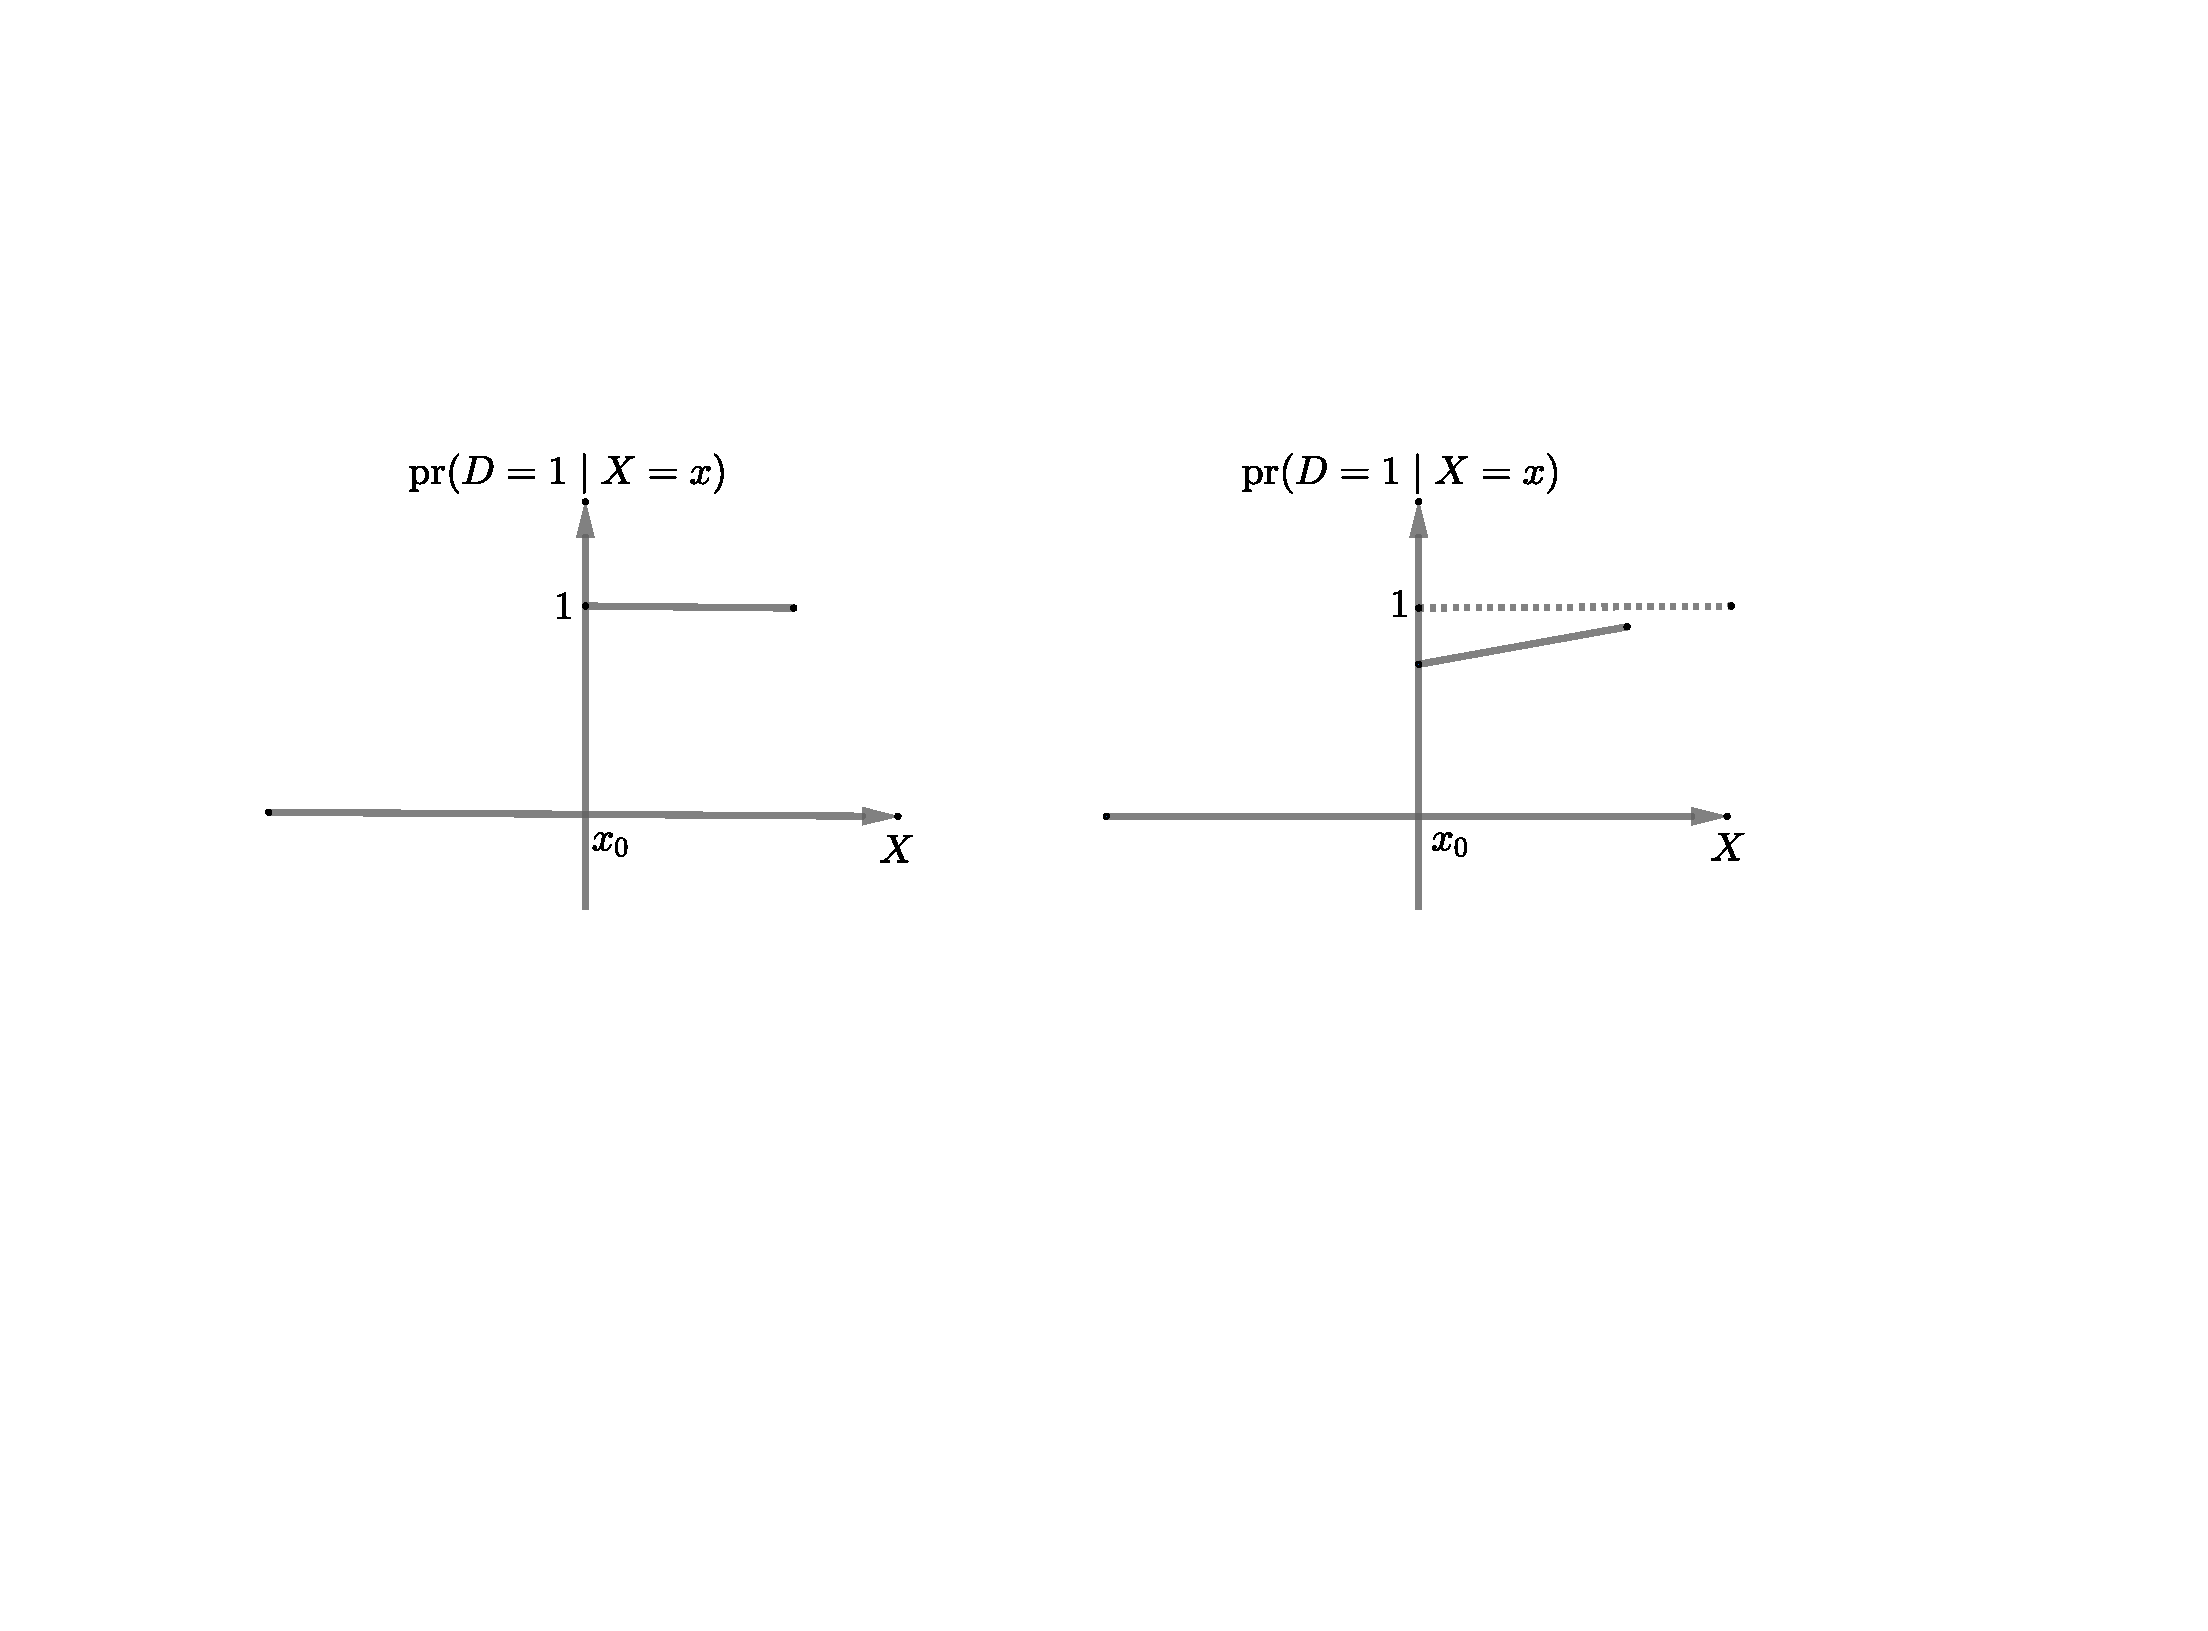
\includegraphics[width = \textwidth]{figures/RDcompare.pdf}
\caption{严格与模糊回归不连续设计的处理分配差异}\label{fig::rdd-compare}
\end{figure}






令$Y_i$为关注的结果。将$Z_i$视为分配的处理，可定义潜在结果$\{ D_i(1), D_i(0), Y_i(1), Y_i(0) \}$。根据定理\ref{thm::identification-rdd}，$Z$的精确断点回归可识别\begin{eqnarray*}
\tau_D(x_0)  &=& E\{ D(1) - D(0)  \mid X=x_0 \}\\
&=& \lim_{\varepsilon \rightarrow 0+} E( D \mid Z=1, X=x_0+\varepsilon ) - \lim_{\varepsilon \rightarrow 0+} E( D \mid Z=0, X=x_0-\varepsilon )
\end{eqnarray*}和\begin{eqnarray*}
\tau_Y(x_0)  &=& E\{ Y(1) - Y(0)  \mid X=x_0 \}\\
&=& \lim_{\varepsilon \rightarrow 0+} E( Y \mid Z=1, X=x_0+\varepsilon ) - \lim_{\varepsilon \rightarrow 0+} E( Y \mid Z=0, X=x_0-\varepsilon )
\end{eqnarray*}以$Z$作为$D$的工具变量，并在$X = x_0$处施加工具变量假设，即可应用定理\ref{thm::CACE-identification}识别局部依从者平均因果效应。

\begin{theorem}
\label{thm::identification-frdd}
假设处理由$Z = I(X \geq x_0)$决定，其中$x_0$为预定阈值。在$x_0$的无穷小邻域内，假设单调性$$
D_i(1) \geq D_i(0)
$$和排除限制$$
D_i(1) = D_i(0) \Longrightarrow  Y_i(1) = Y_i(0) 
$$成立。局部依从者平均因果效应定义为$$
 \tau_\cp(x_0)   
= E\{ Y(1) - Y(0)  \mid D(1)  >  D(0),  X=x_0 \},
$$可以由$$
 \tau_\cp(x_0)   
=  \frac{ E\{ Y(1) - Y(0)  \mid X=x_0 \}  }{E\{ D(1) - D(0)  \mid X=x_0 \}} .
$$识别。进一步假设$E\{ D(1) \mid X=x   \}$和$E\{ Y(1) \mid X=x   \}$在$x=x_0$处右连续，$E\{ D(0) \mid X=x   \}$和$E\{ Y(0) \mid X=x   \}$在$x=x_0$处左连续。若$E(D\mid X=x)$在$x=x_0$处存在非零跳跃，则局部依从者平均因果效应可以由$$
 \tau_\cp(x_0) 
 = \frac{ \lim_{\varepsilon \rightarrow 0+} E( Y \mid Z=1, X=x_0+\varepsilon ) - \lim_{\varepsilon \rightarrow 0+} E( Y \mid Z=0, X=x_0-\varepsilon ) }
{\lim_{\varepsilon \rightarrow 0+} E( D \mid Z=1, X=x_0+\varepsilon ) - \lim_{\varepsilon \rightarrow 0+} E( D \mid Z=0, X=x_0-\varepsilon )}
$$识别。 
\end{theorem}


 定理\ref{thm::identification-frdd}实为定理\ref{thm::identification-rdd}与\ref{thm::CACE-identification}的综合形式。其证明过程留作习题\ref{para::proof-theorem-frd}。 
 

无论严格抑或模糊回归不连续设计，选取断点邻域范围均属核心操作。一般而言，较小邻域能降低偏差却增加方差；较大邻域则反之。这种偏差-方差权衡亟需通过敏感性分析加以权衡。当前已有基于统计判据的自动选择方法，却需满足若干严苛前提条件。因此就实际分析而言，多步调整邻域范围并开展敏感性检验方为稳妥策略。 

假设已用带宽$h$确定$x_0$的邻域。对于满足$X_i \in [x_0-h, x_0 + h]$的数据，可用$$
\hat{\tau}_D(x_0) = \text{the coefficient of } Z_i
\text{ in the OLS fit of } D_i \text{ on } \{1, Z_i, R_i, L_i\},
$$估计$\tau_D(x_0) $，用$$
\hat{\tau}_Y(x_0) = \text{the coefficient of } Z_i
\text{ in the OLS fit of } Y_i \text{ on } \{1, Z_i, R_i, L_i\},
$$估计$\tau_Y(x_0) $，其中回顾定义$R_i = \max(X_i - x_0, 0)$和$L_i= \min (X_i - x_0, 0)$。于是局部依从者平均因果效应可估计为$$
\hat\tau_\cp(x_0)  = \hat{\tau}_Y(x_0) / \hat{\tau}_D(x_0).
$$这是间接最小二乘估计量。由定理\ref{thm::ils=2sls}，它在数值上等于$$
\text{the coefficient of } D_i
\text{ in the TSLS fit of } Y_i \text{ on } \{1, D_i, R_i, L_i\}  
$$其中用$Z_i$作为$D_i$的工具变量。总之，选定$h$后，$ \tau_\cp(x_0)$的估计就归结为对阈值附近的局部数据实施两阶段最小二乘。  


\section{应用示例}
 \label{sec::application-frdd}

\subsection{再分析 \citet{asher2020rural} 的数据}
\label{sec::indian-road-data}

重新考察例\ref{eg::indianroad}。对于一系列$h$，可使用结果变量\ri{occupation_index_andrsn}计算点估计和标准误。 
\begin{lstlisting}
library("car")
road_dat = read.csv("indianroad.csv")
table(road_dat$t, road_dat$r2012)
road_dat$runv = road_dat$left + road_dat$right
## sensitivity analysis 
seq.h  = seq(10, 80, 1)
frd_sa = lapply(seq.h, function(h){
  road_sub = subset(road_dat, abs(runv)<=h)
  road_sub$r2012hat = lm(r2012 ~ t + left + right,
                         data = road_sub)$fitted.values
  tslsreg = lm(occupation_index_andrsn ~ r2012hat + left + right,
               data = road_sub)
  res = with(road_sub,
             {
               occupation_index_andrsn -
                 cbind(1, r2012, left, right)%*%coef(tslsreg)
             })
  tslsreg$residuals = as.vector(res)
  
  c(coef(tslsreg)[2],
    sqrt(hccm(tslsreg, type = "hc2")[2, 2]),
    length(res))
})
frd_sa = do.call(rbind, frd_sa)
\end{lstlisting}
图\ref{fig::indian_road}呈现了分析结果：仅当 $h$ 取值较大时才出现显著处理效应。 

\begin{figure}
\centering
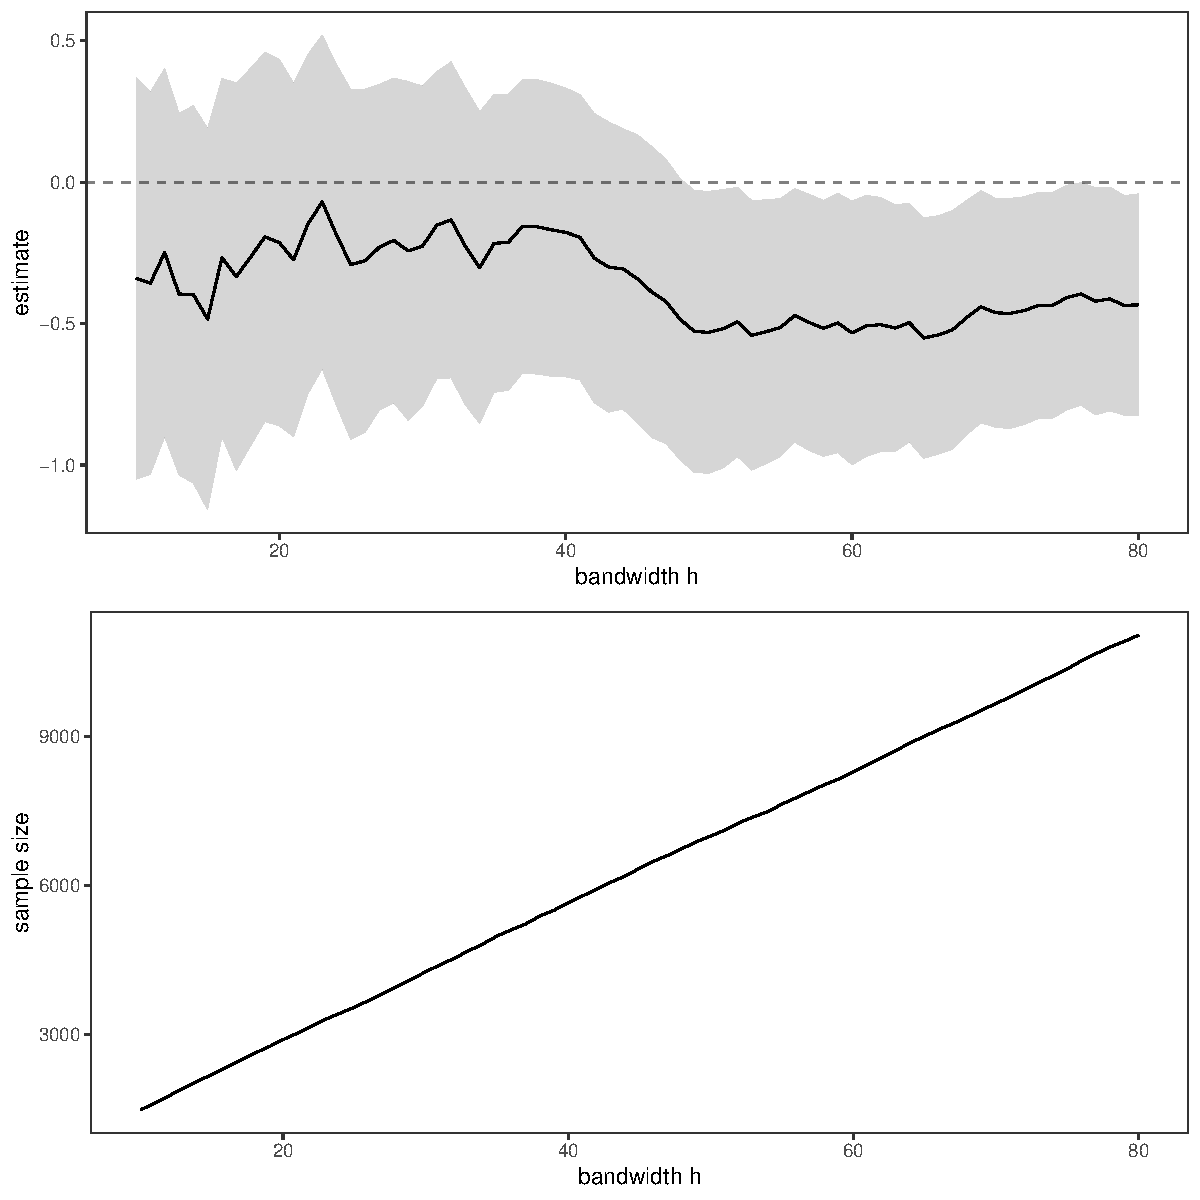
\includegraphics[width = 0.9\textwidth]{figures/frd_indian.pdf}
\caption{基于两步法再分析\citet{asher2020rural}数据所得点估计与标准误}
\label{fig::indian_road}
\end{figure} 


\ri{rdrobust}包可自动确定最优带宽。分析结果显示新建道路并未对目标指标产生明显影响。 

\begin{lstlisting}
> library("rdrobust")
> frd_road = with(road_dat,
+                 {
+                   rdrobust(y = occupation_index_andrsn,
+                            x = runv,
+                            c = 0,
+                            fuzzy = r2012)
+                 })
> res = cbind(frd_road$coef, frd_road$se)
> round(res, 3)
                Coeff Std. Err.
Conventional   -0.253     0.301
Bias-Corrected -0.283     0.301
Robust         -0.283     0.359
\end{lstlisting}

\subsection{再分析 \citet{li2015evaluating} 的数据}
 \label{sec::italian-university}
 
 
 重新考察例\ref{eg::italianuniversity}。运行变量为15,000减去标准化收入。在分析中，将数据限制为运行变量位于$[-5,000,5,000]$内的子集，再将运行变量除以$5,000$，使其取值限制于$[-1,1]$，阈值为零。下面计算一系列$h$对应的点估计和标准误。 
\begin{lstlisting}
library("car")
italy = read.csv("italy.csv")
italy$left  = pmin(italy$rv0, 0)
italy$right = pmax(italy$rv0, 0)
## sensitivity analysis 
seq.h  = seq(0.1, 1, 0.01)
frd_sa = lapply(seq.h, function(h){
  italy_sub = subset(italy, abs(rv0)<=h)
  italy_sub$Dhat = lm(D ~ Z + left + right,
                      data = italy_sub)$fitted.values
  tslsreg = lm(outcome ~ Dhat + left + right,
               data = italy_sub)
  res = with(italy_sub,
             {
               outcome -
                 cbind(1, D, left, right)%*%coef(tslsreg)
             })
  tslsreg$residuals = as.vector(res)
  
  c(coef(tslsreg)[2],
    sqrt(hccm(tslsreg, type = "hc2")[2, 2]),
    length(res))
})
frd_sa = do.call(rbind, frd_sa)
 \end{lstlisting}
 


  图\ref{fig::italy_university}显示测算数据：无论何种带宽设置，助学金对辍学率均无明显效应。 
\begin{figure}
\centering
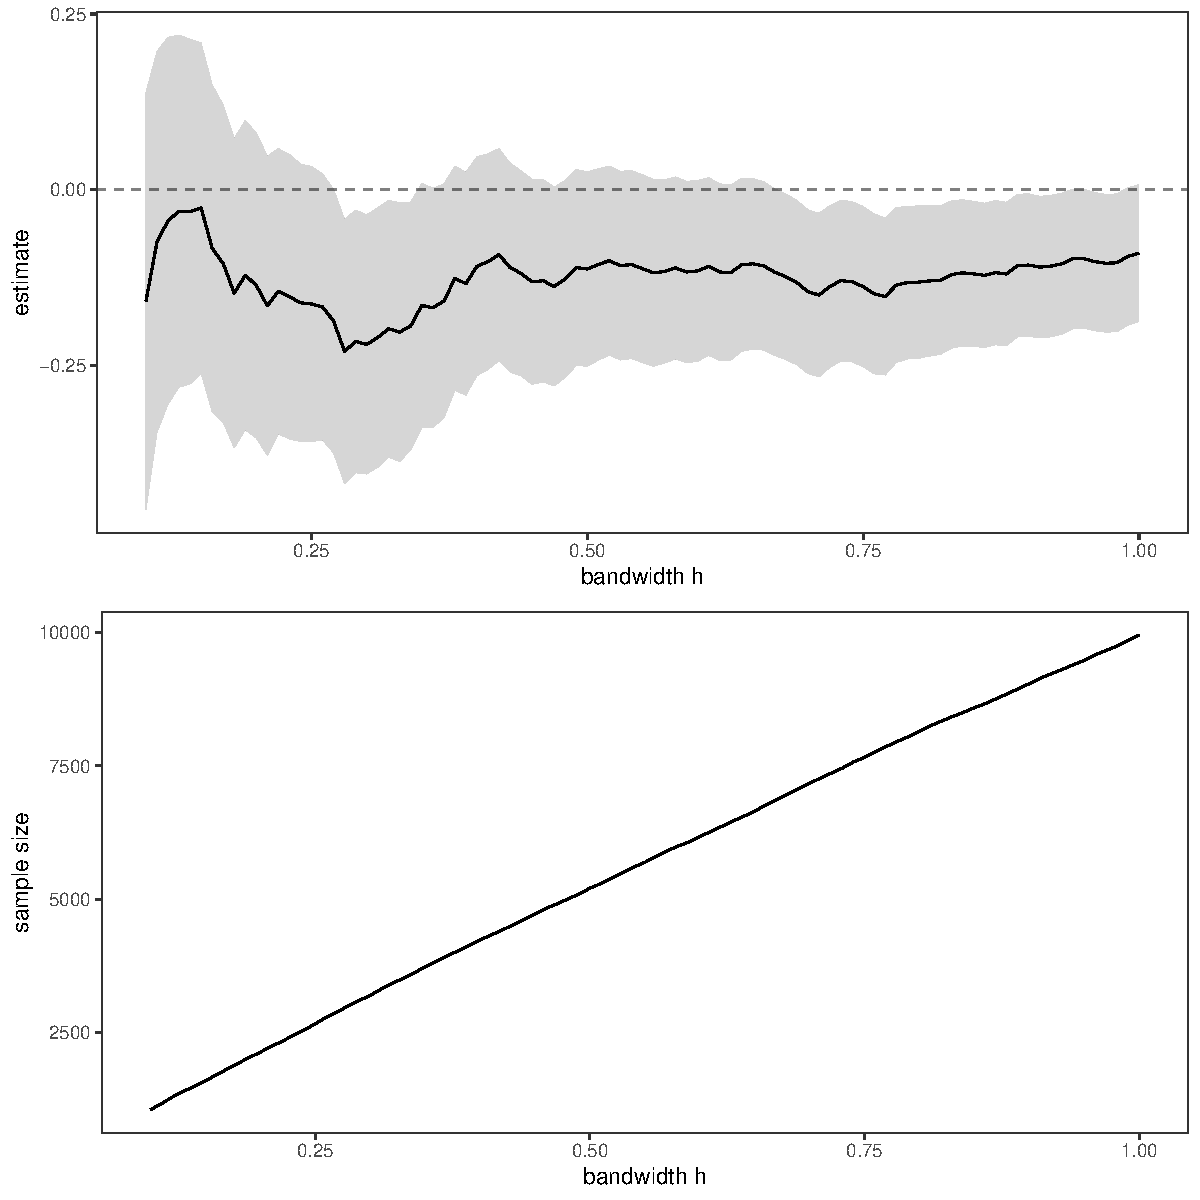
\includegraphics[width = 0.9\textwidth]{figures/frd_italy.pdf}
\caption{基于两步法再分析\citet{li2015evaluating}数据所得点估计及标准误}
\label{fig::italy_university}
\end{figure} 
 
 
 
使用\ri{rdrobust}包得到的结果也支持相同结论。 
 
 \begin{lstlisting}
> library("rdrobust")
> frd_italy = with(italy,
+                  {
+                    rdrobust(y = outcome,
+                             x = rv0,
+                             c = 0,
+                             fuzzy = D)
+                  })
> res = cbind(frd_italy$coef, frd_italy$se)
> round(res, 3)
                Coeff Std. Err.
Conventional   -0.149     0.101
Bias-Corrected -0.155     0.101
Robust         -0.155     0.121
 \end{lstlisting}
 
 
 
 \section{讨论}


第\ref{chapter::overlap}章与本章均基于运行变量条件下潜在结果期望值的连续性来构建回归不连续分析框架。此视角虽具数学简洁性，却仅能在断点处精确估计局部效应。\citet{hahn2001identification}开拓了这一研究方向。 

另一种较少采用的视角基于{\it 局部随机化}\citep{cattaneo2015randomization, li2015evaluating}。若将运行变量看作某个潜在真实量的含噪测量，且阈值的选取带有一定任意性，则阈值附近的单位不存在系统差异。这提示，在阈值的小邻域内，各单位像随机实验中一样随机接受处理或对照。类似于第一种视角中选择$h$的问题，这里关键在于确定断点附近多大的范围可以视为随机实验。将这种直觉用数学量化并不容易，因此，在第二种视角下，对一系列$h$开展敏感性分析同样是合理的做法。  


关于回归不连续设计的概念探讨可参考\citet{sekhon2017interpreting}。 



 
\section{作业习题}

\paragraph{定理 \ref{thm::identification-frdd} 的证明}\label{para::proof-theorem-frd}

试证明定理\ref{thm::identification-frdd}。 


\paragraph{数据分析}
 
前文\ref{sec::indian-road-data}已针对指标\ri{occupation_index_andrsn}做了分析。其他相关指标包括\ri{transport_index_andrsn}、\ri{firms_index_andrsn}、\ri{consumption_index_andrsn}与\ri{agriculture_index_andrsn}；它们的物理意义均见原研究文献。请同样测算各变量所受影响程度。 

 

\paragraph{关于\citet{li2015evaluating}分析思路的思考}
\label{problem::italy-srd}

\citet{li2015evaluating}的研究中关键变量为二值申请状态 $A$，其对应潜在结果 $A(1)$ 与 $A(0)$ 分别对应于处理组 $Z=1$ 与对照组 $Z=0$。依定义：
$$
D(1) = A(1), \quad D(0) = 0,
$$
因此符合“顺从者”条件的个体 $\{ D(1), D(0) \} = (1,0)$ 等价于 $A(1) = 1$。这意味着
$$
\tau_\cp(x_0) = E\{ Y(1) - Y(0) \mid A(1) = 1, X = x_0 \}. 
$$
例\ref{sec::italian-university}中分析采用全部样本测定 $\tau_\cp(x_0)$。 

另一种分析是只使用满足$A=1$的单位。此时处理状态由$X$决定，但这种分析可能存在问题，因为\begin{eqnarray}
&& \lim_{\varepsilon \rightarrow 0+} E\{ Y \mid A  = 1, X = x_0 + \varepsilon \} -\lim_{\varepsilon \rightarrow 0+}  E\{ Y \mid A  = 1, X = x_0- \varepsilon  \}  \nonumber  \\
&=& E\{ Y(1) \mid A(1)  = 1,   X = x_0   \} -  E\{ Y(0) \mid A(0)  = 1,   X = x_0   \} .\label{hw::frdd-florence-A=1}
\end{eqnarray}证明\eqref{hw::frdd-florence-A=1}，并解释这种分析为何可能有问题。


说明：\eqref{hw::frdd-florence-A=1}左端是在$A=1$条件下、$X=x_0$处局部平均处理效应的识别公式。\eqref{hw::frdd-florence-A=1}右端则分别是满足$(A(1)  = 1,   X = x_0 )$和$(A(0)  = 1,   X = x_0)$的两个子组的潜在结果均值之差。相关讨论见后面的第\ref{chapter::principal-stratification}章。 
 


 
 \paragraph{推荐阅读}

\citet{imbens2008regression}以潜在结果视角提供了实用分析指引；\citet{lee2010regression}则综述了回归不连续设计在经济学中的应用发展。 
   
         
\chapter{工具变量方法的应用：孟德尔随机化}
 \label{chapter::iv-mr}




\citet{katan1986apoupoprotein}研究了某些观察性研究的结果，这些研究表明低血清胆固醇水平与癌症风险相关。然而，正如我们所讨论的，观察性研究容易受到未测量混杂因素的影响。因此，很难将观察到的关联性解释为因果关系。在\citet{katan1986apoupoprotein}所研究的具体问题中，甚至有可能是癌症的早期阶段导致了血清胆固醇水平降低。利用常规的流行病学研究方法，要厘清血清胆固醇水平对癌症的因果效应似乎是个难题。\citet{katan1986apoupoprotein}指出，载脂蛋白E基因与血清胆固醇水平相关，但并不直接影响癌症的发生。因此，如果低血清胆固醇水平确实会导致癌症，那么在具有该基因型的人群与不具备该基因型的人群之间，其癌症风险应当存在显著差异。用因果推断的术语来说，\citet{katan1986apoupoprotein}提出将载脂蛋白E基因作为工具变量来使用。 


\citet{katan1986apoupoprotein}并未开展数据分析，只是提出了一种概念性设计，以同时应对{\it 未测量混杂}和{\it 反向因果}。此后，得益于现代全基因组关联研究，人们开展了更复杂精细的研究。这些研究将遗传信息作为流行病学研究中暴露的工具变量，估计暴露对结果的因果效应。其思想均源于{\it 孟德尔第二定律}，即{\it 自由组合定律}，它指出一种性状的遗传独立于其他性状的遗传。因此，使用遗传信息作为工具变量的方法称为{\it 孟德尔随机化}（MR）。 


\section{背景与动机}

从图表上看，图\ref{fig::mr-dag}呈现了处理因素$D$、结局变量$Y$、未测量混杂因素$U$以及遗传工具变量$G_1, \ldots, G_p$之间的因果关系。在多数MR研究中，这些遗传工具变量往往是单核苷酸多态性位点（SNP）。由于多效性现象的存在\footnote{多效性是指一个基因可同时影响两个或多个看似无关的表型特征}，这些遗传工具变量也可能直接影响目标结局。因此，图\ref{fig::mr-dag}也考虑了排除性假设可能被违反的情形。  

\begin{figure}
\centering
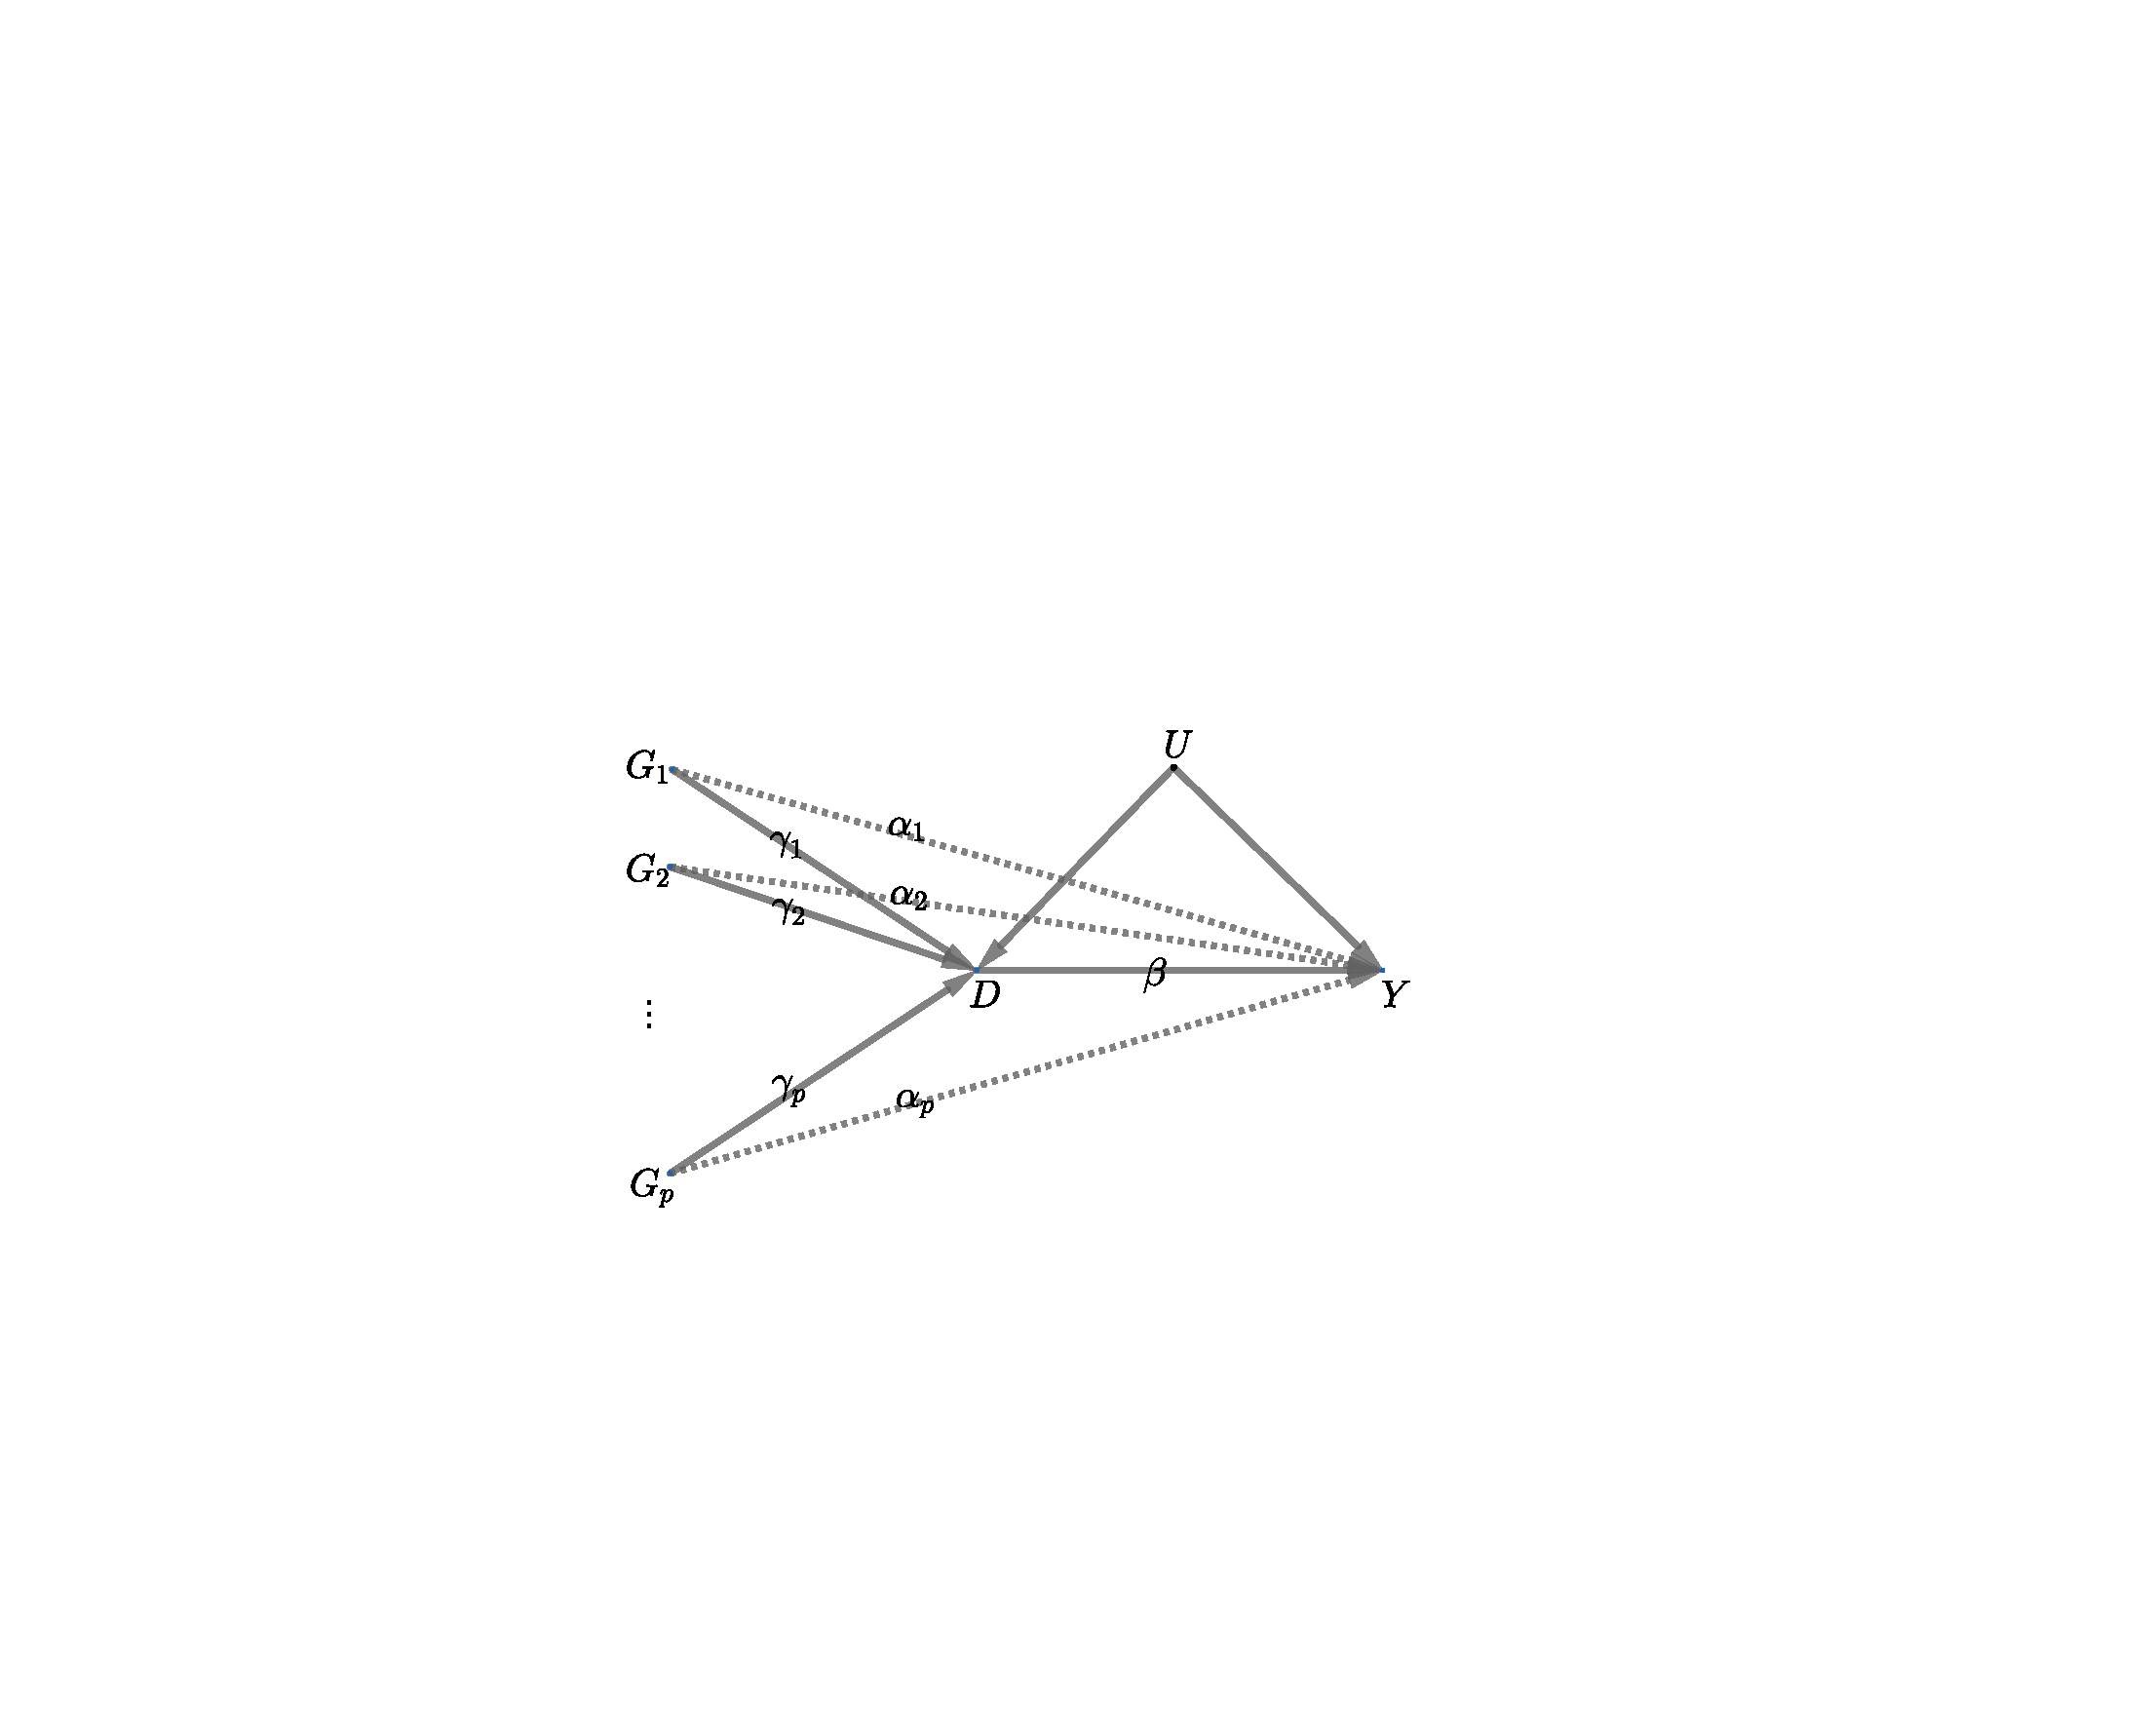
\includegraphics[width = 0.8 \textwidth]{figures/mr_dag.pdf}
\caption{孟德尔随机化的因果图}\label{fig::mr-dag}
\end{figure}



标准的线性工具变量模型通常假设工具变量对结局无直接效应。下面的定义\ref{def::linear-iv-model-mr}分别给出了该模型的结构形式及简化形式。 

\begin{definition}
[线性工具变量模型]\label{def::linear-iv-model-mr}
标准线性工具变量模型\begin{eqnarray}
Y  &=& \beta_0 +  \beta D + \beta_u U + \varepsilon_Y , \\
D  &=& \gamma_0 +   \gamma_1 G_1 + \cdots + \gamma_p G_p + \gamma_u U + \varepsilon_D ,
\end{eqnarray}的简约式为\begin{eqnarray}
Y  &=&\beta_0 +  \beta  \gamma_0 + \beta \gamma_1 G_1 + \cdots + \beta  \gamma_p G_p  + (\beta_u + \beta_0 \gamma_u )U + \varepsilon_Y , \\
D  &=& \gamma_0 +  \gamma_1 G_1 + \cdots + \gamma_p G_p + \gamma_u U + \varepsilon_D ,
\end{eqnarray}
\end{definition}



定义\ref{def::linear-model-invalid-iv-mr}则允许排除性假设被违反的情况；在此情形下，$G_1, \ldots, G_p$便不再符合有效工具变量的条件。 


\begin{definition}
[可能存在无效工具变量的线性模型]\label{def::linear-model-invalid-iv-mr}
线性模型\begin{eqnarray}
Y  &=& \beta_0 + \beta D + \alpha_1 G_1 + \cdots + \alpha_p G_p  + \beta_u U + \varepsilon_Y ,   \\
D  &=& \gamma_0 + \gamma_1 G_1 + \cdots + \gamma_p G_p + \gamma_u U + \varepsilon_D ,
\end{eqnarray}的简约式为\begin{eqnarray}
Y  &=& ( \beta_0 +\beta  \gamma_0 ) +  (\alpha_1 + \beta \gamma_1)  G_1 + \cdots + (\alpha_p +  \beta  \gamma_p) G_p \nonumber  \\
&&+  ( \beta_u + \beta \gamma_u )  U + \varepsilon_Y ,   \\
D  &=& \gamma_0 +  \gamma_1 G_1 + \cdots + \gamma_p G_p + \gamma_u U + \varepsilon_D .
\end{eqnarray}
\end{definition}

定义\ref{def::linear-iv-model-mr}与\ref{def::linear-model-invalid-iv-mr}与第\ref{chapter::iv-econometric}章中介绍的线性工具变量模型略有差异，它们显式地引入了混杂因素$U$；不过这一细微差别并未从本质上改变讨论框架。 


在符合排除性假设的定义\ref{def::linear-iv-model-mr}中，我们有：
$$
\Gamma_j = \beta \gamma_j,\quad (j=1,\ldots,p).
$$
而在排除性假设被违反时，即定义\ref{def::linear-model-invalid-iv-mr}中，则有：
$$
\Gamma_j = \alpha_j +   \beta \gamma_j,\quad (j=1,\ldots,p). 
$$



若有个体数据，可在定义\ref{def::linear-iv-model-mr}中的线性工具变量模型下，用经典两阶段最小二乘估计量估计$\beta$。然而，大多数MR研究只有来自多个全基因组关联研究的汇总统计量，没有个体数据。典型的汇总统计量MR研究具有以下数据结构。


\begin{assumption}
[基于汇总统计量的孟德尔随机化研究]\label{assume::MR-summary}
(a)
我们可获得处理因素与遗传工具变量之间的回归系数$\hat{\gamma}_1   , \ldots, \hat{\gamma}_p$，以及对应的标准误$\se_{D1}, \ldots, \se_{Dp}$。假设：
\begin{eqnarray}
\label{eq::small-gammas}
\hat{\gamma}_1  \rightarrow \gamma_1 , \ldots, \hat{\gamma}_p \rightarrow \gamma_p
\end{eqnarray}
在概率意义上成立，且忽略标准误的不确定性。 

(b) 已知结果对遗传工具变量的回归系数$\hat{\Gamma}_1   , \ldots, \hat{\Gamma}_p$及其标准误$\se_{Y1}, \ldots, \se_{Yp}.$。假设\begin{eqnarray}
\label{eq::big-gammas}
\hat{\Gamma}_1 \rightarrow \Gamma_1 , \ldots, \hat{\Gamma}_p \rightarrow \Gamma_p
\end{eqnarray}依概率成立，并忽略标准误中的不确定性。  

(c)
假设$\hat{\gamma}_1   , \ldots, \hat{\gamma}_p, \hat{\Gamma}_1   , \ldots, \hat{\Gamma}_p$均为联合正态分布且彼此独立。
\end{assumption}


%\begin{eqnarray}
%\label{eq::small-gammas}
%\hat{\gamma}_1  \rightarrow \gamma_1 , \ldots, \hat{\gamma}_p \rightarrow \gamma_p
%\end{eqnarray}
%in probability with standard errors
%\begin{eqnarray}
%\label{eq::small-gammas-se}
%\se_{D1}, \ldots, \se_{Dp},
%\end{eqnarray}
%and the regression coefficients of the outcome on  the  genetic IVs:
%\begin{eqnarray}
%\label{eq::big-gammas}
%\hat{\Gamma}_1 \rightarrow \Gamma_1 , \ldots, \hat{\Gamma}_p \rightarrow \Gamma_p
%\end{eqnarray}
%in probability with standard errors
%\begin{eqnarray}
%\label{eq::big-gammas-se}
%\se_{Y1}, \ldots, \se_{Yp}.
%\end{eqnarray}

回归系数的渐近正态性可以由中心极限定理说明。在大样本中，标准误估计准确地估计真实标准误。因此，唯一较微妙的假设是各回归系数联合独立。$\hat{\gamma}_j$与$\hat{\Gamma}_j$之间的独立性是合理的，因为它们通常基于不同样本计算。 

若各$G_j$独立，且$D$的真实线性模型具有同方差误差项，则各$\hat{\gamma}_j$之间的独立性可能合理，见第\ref{section::linear-model-var}章。但当线性模型误差项存在异方差时，这个假设就变得微妙。若各$G_j$不独立，就很难说明估计量相互独立。若回归系数来自非线性模型，则更难说明这种独立性。各$\hat{\Gamma}_j$之间的独立性可作类似讨论。 

本章重点讨论如何根据假设\ref{assume::MR-summary}中的上述汇总统计量，对$\beta$进行统计推断。 



\section{基于汇总统计量的孟德尔随机化}


\subsection{固定效应估计量}\label{sec::mr-fixed-effect}


在定义\ref{def::linear-iv-model-mr}下，$\alpha_j = 0$，故对所有$j$有$\beta = \Gamma_j / \gamma_j$。一种简单的方法是所谓的{\it 元分析}\citep{bowden2018improving}：将多个估计量$\hat{\beta}_j =  \hat \Gamma_j / \hat\gamma_j$合并，用于估计共同参数$\beta$，也称固定效应。利用delta方法，见例\ref{thm::delta-method}，比率估计量$\hat{\beta}_j$的近似标准误平方为$$
\se_j^2 = (\se_{Yj}^2 + \hat{\beta}_j^2\se_{Dj}^2  )    / \hat\gamma_j^2.
$$因此，用于估计$\beta$的最优线性组合是基于方差倒数的Fisher加权，见习题\ref{hw::fisher-weighting}：$$
\hat{\beta}_{\text{fisher}0} =  \frac{ \sum_{j=1}^p  \hat{\beta}_j  / \se_j^2  }{ \sum_{j=1}^p 1  / \se_j^2 }
$$其方差为$(\sum_{j=1}^p 1  / \se_j^2)^{-1} $。若忽略$\hat\gamma_j$中由$\se_{Dj}$量化的不确定性，估计量简化为$$
\hat{\beta}_{\text{fisher}1} =  \frac{ \sum_{j=1}^p  \hat{\beta}_j  \hat\gamma_j^2 /  \se_{Yj}^2 }{ \sum_{j=1}^p   \hat\gamma_j^2 /  \se_{Yj}^2 }
=\frac{ \sum_{j=1}^p  \hat \Gamma_j   \hat\gamma_j /  \se_{Yj}^2 }{ \sum_{j=1}^p   \hat\gamma_j^2 /  \se_{Yj}^2 },
$$其方差为$( \sum_{j=1}^p   \hat\gamma_j^2 /  \se_{Yj}^2 )^{-1}$。虽然实践中更常使用$\hat{\beta}_{\text{fisher}1} $，但基于它的推断并非最优\citep{bowden2018improving}。$\hat{\beta}_{\text{fisher}0}$和$\hat{\beta}_{\text{fisher}1}$都称为{\it 固定效应估计量}。 


考虑虽非最优但较简单的估计量$\hat{\beta}_{\text{fisher}1}$。在定义\ref{def::linear-model-invalid-iv-mr}下，可以证明$$
\hat{\beta}_{\text{fisher}1}  \rightarrow 
\frac{ \sum_{j=1}^p   \Gamma_j    \gamma_j /  \se_{Yj}^2 }{ \sum_{j=1}^p    \gamma_j^2 /  \se_{Yj}^2 }
= \beta + \frac{ \sum_{j=1}^p   \alpha_j    \gamma_j /  \se_{Yj}^2 }{ \sum_{j=1}^p    \gamma_j^2 /  \se_{Yj}^2 }
$$依概率成立。若对所有$j$都有$\alpha_j = 0$，则$\hat{\beta}_{\text{fisher}1} $一致。即使这个条件不成立，只要$\alpha_j  $和$  \gamma_j$以$ 1/  \se_{Yj}^2$加权的内积为零，$\hat{\beta}_{\text{fisher}1}  $仍可能一致。当遗传工具变量很多，且表示排除限制违反程度的$\alpha_j$是从均值为零的分布独立随机抽取时，就可满足这种条件。 


\subsection{埃格回归法}


从定义\ref{def::linear-iv-model-mr}出发，真实参数满足$$
\Gamma_j = \beta \gamma_j \quad (j=1,\ldots, p);
$$对于估计值，上述恒等式仅近似成立：$$
\hat \Gamma_j \approx  \beta \hat \gamma_j \quad (j=1,\ldots, p).
$$这看起来像经典的将$\{\hat \Gamma_j \}_{j=1}^p$对$\{\hat \gamma_j \}_{j=1}^p$回归的最小二乘问题。可以将$\hat \Gamma_j$对$\hat \gamma_j$作带截距或不带截距的WLS拟合，可用$w_j$作为权重，以估计$\beta$。由第\ref{sec::appendix-wls}章回顾的WLS代数性质，可得到以下结果。 


不含截距时，$\hat \gamma_j$的系数为$$
\hat{\beta}_{\text{egger}1}  = \frac{  \sum_{j=1}^p  \hat \gamma_j  \hat \Gamma_j w_j     }{ \sum_{j=1}^p  \hat \gamma_j ^2 w_j },
$$若$w_j =  1/\se_{Yj}^2$，它就化为$\hat{\beta}_{\text{fisher}1} $。这种WLS方法称为{\it Egger回归}，比第\ref{sec::mr-fixed-effect}节的固定效应估计量更一般。包含截距时，$\hat \gamma_j$的系数为$$
\hat{\beta}_{\text{egger}0}  =  \frac{  \sum_{j=1}^p  (\hat \gamma_j  - \hat \gamma_w) (\hat \Gamma_j - \hat \Gamma_w) w_j     }
{ \sum_{j=1}^p  (\hat \gamma_j  - \hat \gamma_w) ^2 w_j }
$$其中$\hat \gamma_w = \sum_{j=1}^p \hat \gamma_j w_j /  \sum_{j=1}^p   w_j  $和$\hat \Gamma_w = \sum_{j=1}^p \hat \Gamma_j w_j /  \sum_{j=1}^p   w_j  $分别为各$\hat \gamma_j$和各$\hat \Gamma_j$的加权平均。 





在定义\ref{def::linear-model-invalid-iv-mr}下，即使不假设所有$\alpha_j$都为零，也有$$
\hat{\beta}_{\text{egger}0} \rightarrow 
\frac{  \sum_{j=1}^p  (  \gamma_j  -   \gamma_w) ( \Gamma_j -   \Gamma_w) w_j     }
{ \sum_{j=1}^p  (  \gamma_j  -  \gamma_w) ^2 w_j }
=\beta + \frac{  \sum_{j=1}^p  (  \gamma_j  -   \gamma_w) ( \alpha_j -   \alpha_w) w_j     }
{ \sum_{j=1}^p  (  \gamma_j  -  \gamma_w) ^2 w_j }
$$依概率成立，其中$\gamma_w, \Gamma_w$和$\alpha_w$分别为相应真实参数的加权平均。因此，只要将$\alpha_j$对$\gamma_j$作WLS回归所得的系数为零，$\hat{\beta}_{\text{egger}0} $就是$\beta$的一致估计量。这弱于对所有$j$要求$\alpha_j=0$。若$\gamma_j$和$\alpha_j$为相互独立随机变量的实现值，则可满足这一较弱条件，称为工具强度独立于直接效应（Instrument Strength Independent of Direct Effect，InSIDE）假设\citep{bowden2015mendelian}。更有趣的是，Egger回归的截距为$$
\hat{\alpha}_{\text{egger}0}  = \hat \Gamma_w - \hat{\beta}_{\text{egger}0}  \hat \gamma_w,
$$在InSIDE假设下依概率收敛于$$
\Gamma_w -  \beta  \gamma_w = \alpha_w
$$因此，截距估计了直接效应的加权平均。 


\section{实例演示}
\label{sec::mr-examples}

首先给出实现费舍尔加权的函数。
 \begin{lstlisting}
fisher.weight = function(est, se)
{
  n = sum(est/se^2)
  d = sum(1/se^2)
  res = c(n/d, sqrt(1/d))
  names(res) = c("est", "se")
  res
}
\end{lstlisting}

这里用\ri{mr.raps}包\citep{zhao2020statistical}中的\ri{bmi.sbp}数据，说明基于不同方差估计的Fisher加权。$\hat{\beta}_{\text{fisher}0} $和$\hat{\beta}_{\text{fisher}1} $得到的结果相近。 
 \begin{lstlisting}
> bmisbp = read.csv("mr_bmisbp.csv")
> bmisbp$iv      = with(bmisbp, beta.outcome/beta.exposure)
> bmisbp$se.iv   = with(bmisbp, se.outcome/beta.exposure)
> bmisbp$se.iv1  = with(bmisbp,
+                       sqrt(se.outcome^2 + iv^2*se.exposure^2)/beta.exposure)
> fisher.weight(bmisbp$iv, bmisbp$se.iv)
       est         se 
0.31727680 0.05388827 
> fisher.weight(bmisbp$iv, bmisbp$se.iv1)
       est         se 
0.31576007 0.05893783
\end{lstlisting}


无论是否包含截距项，埃格回归均产生极为相近的估计值；不过其标准误与费舍尔加权法所得结果迥异。 
\begin{lstlisting}
> mr.egger = lm(beta.outcome ~ 0 + beta.exposure,
+               data = bmisbp,
+               weights = 1/se.outcome^2)
> summary(mr.egger)$coef
               Estimate Std. Error  t value    Pr(>|t|)
beta.exposure 0.3172768  0.1105994 2.868704 0.004681659
> 
> mr.egger.w = lm(beta.outcome ~ beta.exposure,
+                 data = bmisbp,
+                 weights = 1/se.outcome^2)
> summary(mr.egger.w)$coef 
                  Estimate  Std. Error    t value    Pr(>|t|)
(Intercept)   0.0001133328 0.002079418 0.05450217 0.956603931
beta.exposure 0.3172989306 0.110948506 2.85987564 0.004811017
 \end{lstlisting}
 
 
图\ref{fig::bmi-sdp-egger}展示了原始数据及带有截距项的埃格回归拟合线。 
 
\begin{figure}
\centering
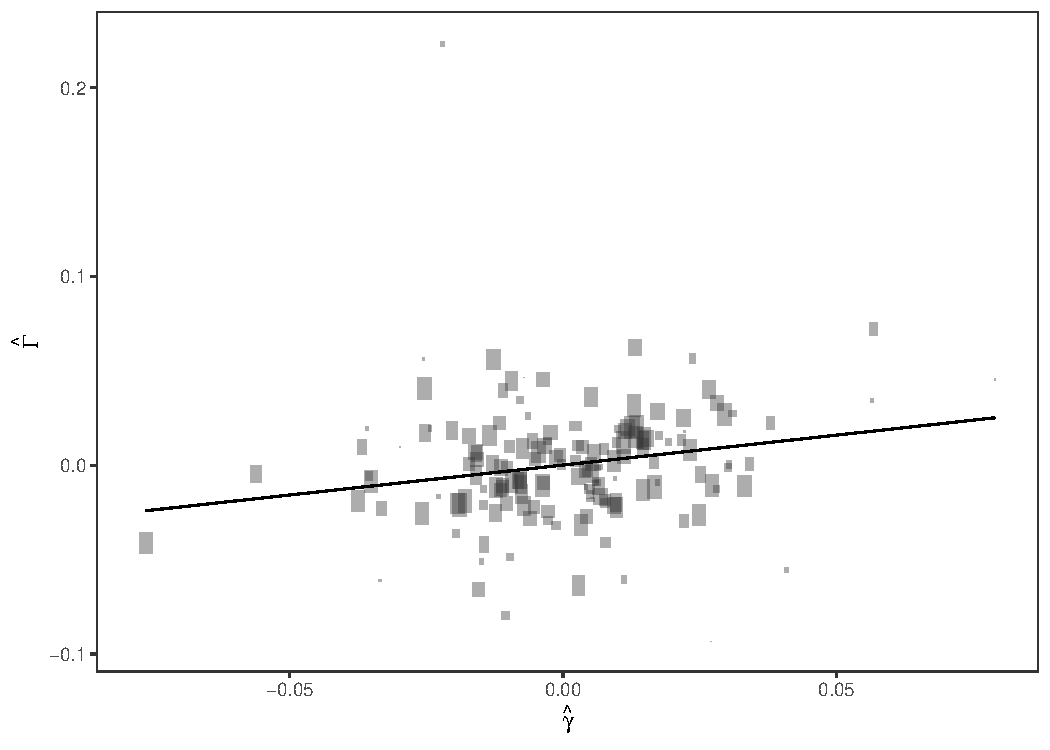
\includegraphics[width = \textwidth]{figures/MR_bmi_sdp.pdf}
\caption{按方差倒数加权的散点图及埃格回归线}\label{fig::bmi-sdp-egger}
\end{figure} 

 
\section{对孟德尔随机化分析法的若干批评}




孟德尔随机化是工具变量思想的具体应用，但其实施需满足诸多较强假设。下文从概念、生物学及技术三个层面对其进行评述。 



在概念层面，多数孟德尔随机化研究中的“处理因素”并未基于潜在结果框架予以清晰界定。例如，研究常将胆固醇水平或身体质量指数视为处理因素，然而它们均为复合变量，其对应的理想化实验定义方式亦不止一种；此时“无干扰无干扰无干扰无干扰”（SUTVA）假设往往难以满足。相关讨论可参见第\ref{chapter::potential-outcomes}章。 


从生物学角度而言，工具变量分析所需的基本前提可能并不成立。孟德尔第二定律虽保证了不同性状遗传的独立性，却未确保所选工具变量与处理因素和结局间的隐性混杂因素互不相关；事实上工具变量亦可能直接影响混杂因素，或某些未被测定的基因同时影响工具变量与混杂因素。此外，该定律亦无法保障排除性假设；工具变量还可能通过非处理因素作用路径影响结局。 


从技术上说，MR的统计假设相当强。线性工具变量模型显然是一个很强的建模假设。各$\hat\gamma_j$和各$\hat\Gamma_j$相互独立的假设也相当强。数据收集过程中的其他问题会进一步使工具变量假设的解释复杂化。例如，处理和结果通常带有测量误差，全基因组关联研究通常采用病例—对照设计，按结果进行抽样，见第\ref{sec::case-control}章。

 
\citet{vanderweele2014methodological}撰写了关于孟德尔随机化方法学挑战的优秀综述文献。 

 
 
\section{作业习题}

\paragraph{数据分析}\label{para::data-bmi-bmi}
分析\ri{R}包\ri{mr.raps}中的\ri{bmi.bmi}数据。更多细节见该包及\citet[][Section 7.2]{zhao2020statistical}。 


 
 \paragraph{推荐阅读}

\citet{davey2003mendelian}系统梳理了孟德尔随机化的优势及局限。 




   

 

\part{涉及处理后变量的因果机制}\label{part::post-treatmentvariable}
 
  
\chapter{主分层法}
 \label{chapter::principal-stratification}

本书的第\ref{part::rcts}至第\ref{part::instrumentalvariables}部分着重探讨干预措施对结果变量的因果效应，有时也会对观测到的干预前协变量加以调整。许多实际应用中还存在某种干预后变量 $M$，它出现在干预之后且与结果变量相关联。一个重要的问题就是如何恰当地利用这个干预后变量 $M$。我将先给出几个具有启发意义的实例，之后介绍 \citet{frangakis2002principal} 基于潜在结果模型对该问题的论述。 
 


\section{启发示例}



\begin{example}[不遵从干预者]\label{eg::noncompliance}
在存在不依从的随机实验中，可用$M$表示实际接受的处理。它受到处理分配$Z$的影响，并影响结果$Y$。这里的$M$与第\ref{chapter::iv-experiment}章中的$D$含义相同。
\end{example}


\begin{example}[因死亡导致的数据截断]\label{eq::truncationbydeath}
在针对重症患者的随机试验中，部分患者可能在测定结果变量 $Y$（如生活质量指标）之前便已死亡。此例中的干预后变量 $M$ 即为表示存活状态的二元指标。 
\end{example}




\begin{example}[失业问题]\label{eg::unemployment}
在职业培训项目中，受试者被随机分配到干预组或对照组，并报告自身的就业状态 $M$ 与工资水平 $Y$。此时，$M$ 即为表示就业状况的二元指标。 
\end{example}




\begin{example}
[替代终点]\label{eg::surrogate-endpoints}
在临床试验中，真正感兴趣的结局指标（如30年生存率）需要长期且成本高昂的随访才能获得。因此研究人员通常选择一些易于测量的替代变量。这些变量即被称作“替代终点”。一个实际例子是：在针对HIV感染者的试验中，候选的替代终点 $M$ 即为CD4细胞计数（CD4细胞属于负责抵御感染的白细胞）。 
\end{example}



上面的例\ref{eg::noncompliance}至\ref{eg::surrogate-endpoints}有一个共同点：变量$M$发生在处理之后，且与结果有关。$M$可能位于从$Z$到$Y$的因果路径上，如图\ref{fig::intermediate-diagram}(a) 所示；例\ref{eg::noncompliance}就对应图\ref{fig::intermediate-diagram}(a)。$M$也可能不在从$Z$到$Y$的因果路径上，如图\ref{fig::intermediate-diagram}(b) 所示；例\ref{eq::truncationbydeath}和\ref{eg::unemployment}对应图\ref{fig::intermediate-diagram}(b)。例\ref{eg::surrogate-endpoints}则可能对应图\ref{fig::intermediate-diagram}(a) 或 (b)，取决于所选择的替代终点。 

 


\begin{figure}[h]
\centering
\begin{subfigure}[]{\textwidth}
                \centering
$$
\begin{xy}
\xymatrix{
&& & U \ar[dl]   \ar[dr] \\
Z \ar[rr] \ar@/_1.5pc/[rrrr] & & M\ar[rr] & & Y\\
}
\end{xy}
$$ 
               \caption{$M$ 位于从 $Z$ 到 $Y$ 的因果路径上；$Z$ 为随机分配变量，$U$ 代表未观测到的混杂因子}
        \end{subfigure}%
        
        \begin{subfigure}[]{\textwidth}
                \centering
$$
\begin{xy}
\xymatrix{
&& & U \ar[dl]   \ar[dr] \\
Z \ar[rr] \ar@/_1.5pc/[rrrr] & & M  & & Y\\
}
\end{xy}
$$
                \caption{$M$ 并非位于从 $Z$ 到 $Y$ 的因果路径上；$Z$ 为随机分配变量，$U$ 代表未观测到的混杂因子}
        \end{subfigure}%
        
\caption{包含干预后变量 $M$ 的因果图}\label{fig::intermediate-diagram}
\end{figure}


实际应用中，实际的因果图结构往往比图\ref{fig::intermediate-diagram}所示要复杂得多。本章内容以 \citet{frangakis2002principal} 的论述为基础，且不预先假设具体的因果图结构。





\section{基于干预后变量的条件化处理问题}

处理干预后变量 $M$ 的一种直观方法是将其视为干预前协变量并基于其观测值进行条件化处理。然而，$M$ 与 $X$ 存在本质区别：$M$ 一般会受到干预影响，而 $X$ 则不会。统计实践中亦有经验法则：为评估干预对结果的平均因果效应，数据分析者不应以任何干预后变量作为条件变量 \citep{cochran1957analysis, rosenbaum1984consquences}。基于潜在结果模型理论，\citet{frangakis2002principal} 对此现象作出了如下精辟解释。 

为简化讨论，本章仅以完全随机实验（CRE）情形为例。

\begin{assumption}
[完全随机实验条件下含中间变量]
\label{assume::complete-randomization-withM}
满足以下条件：
$$
Z \ind  \{ M(1), M(0), Y(1), Y(0), X \} . 
$$
\end{assumption}

 
在给定$M= m$后，比较
\begin{equation}
\pr(Y\mid Z=1, M=m)\label{eq::proby|z1m}
\end{equation}
与
\begin{equation}
\pr(Y\mid Z=0, M=m).\label{eq::proby|z0m}
\end{equation}
看似很直观，因为它衡量了处理后变量取值相同时，处理组与对照组结果分布的差异。若$M$是处理前协变量，这样比较可得到合理的亚组效应；但若$M$是处理后变量，解释就会出现问题。在假设\ref{assume::complete-randomization-withM}下，可将\eqref{eq::proby|z1m}和\eqref{eq::proby|z0m}中的概率改写为
\begin{eqnarray*}
\pr(Y\mid Z=1, M=m)  &=& \pr\{ Y(1)\mid Z=1, M(1) = m  \} \\
&=& \pr\{ Y(1)\mid   M(1) = m  \}
\end{eqnarray*}
以及
\begin{eqnarray*}
\pr(Y\mid Z=0, M=m) &=&  \pr\{ Y(0)\mid Z=0, M(0) = m  \} \\
&=& \pr\{ Y(0)\mid   M(0) = m  \} . 
\end{eqnarray*}
因此，在完全随机实验中，比较\eqref{eq::proby|z1m}与\eqref{eq::proby|z0m}，等价于在不同单位子集中比较$Y(1)$与$Y(0)$的分布：只要$Z$影响$M$，满足$M(1) = m$的单位就与满足$M(0) = m$的单位不同。故除非$M(1) = M(0)$，否则给定$M=m$后的比较一般没有因果解释。\footnote{从因果图也能得到相同结论。在图\ref{fig::intermediate-diagram}中，虽然随机化$Z$保证了$Z\ind U$，但以$M$为条件会引入“碰撞点偏差”，导致$Z\nind U$。} 


再来看示例\ref{eg::noncompliance}。在符合单调性假设 $M(1) \geq M(0)$ 的前提下，比较 $\pr(Y\mid Z=1, M=1)$ 与 $\pr(Y\mid Z=0, M=1)$ 相当于比较“遵从者”与“始终接受干预者”在干预组中的潜在结果，而对照组中“始终接受干预者”的潜在结果则作为基准值。这正是问题\ref{problem::as-treated-analysis}第三部分所探讨的内容。 


再看示例\ref{eq::truncationbydeath}。若干预措施能改善患者的生存状况，那么干预组存活病例数将多于对照组。此时，$M(1)=1$ 的患者群体必定比 $M(0)=1$ 的群体更为虚弱，因此仅使用上述条件比较法得出的结果反而会偏向“对照组更有利”的错误结论。 

\section{基于潜在值的条件化处理法}


\citet{frangakis2002principal}提出，以处理后变量的联合潜在取值$U = \{ M(1), M(0) \}$为条件，对某个$(m_1, m_0)$比较
$$
\pr\{  Y(1) \mid M(1) = m_1, M(0) = m_0 \}
$$
和
$$
\pr\{  Y(0) \mid M(1) = m_1, M(0) = m_0 \}
$$
这样比较的是满足$M(1) = m_1$和$ M(0) = m_0$的同一组单位在处理与对照下的潜在结果。\citet{frangakis2002principal}将这种策略称为{\it 主分层}，把$\{ M(1), M(0) \}$看作处理前协变量。据此，定义
$$
\tau(m_1, m_0) = E\{  Y(1) - Y(0) \mid M(1) = m_1, M(0) = m_0\}
$$
为满足$M(1) = m_1, M(0) = m_0$的亚组的主分层平均因果效应。若$M$为二元变量，共有四个亚组：
\begin{equation}
\label{eq::psace}
\left\{ \begin{array}{rcl}
\tau(1,1) &=& E\{  Y(1) - Y(0) \mid M(1) = 1, M(0) =1\} ,\\
\tau(1,0) &=&E\{  Y(1) - Y(0) \mid M(1) = 1, M(0) =0\},\\
\tau(0,1) &=&E\{  Y(1) - Y(0) \mid M(1) = 0, M(0) =1\},\\
\tau(0,0) &=&E\{  Y(1) - Y(0) \mid M(1) = 0, M(0) = 0 \}.
\end{array} 
\right.
\end{equation}
由于$\{ M(1), M(0) \}$不受处理影响，它是协变量，故$\tau(m_1, m_0) $是亚组因果效应。对于满足$M(1) = M(0)$的亚组，处理中间变量的取值不变，所以$\tau(1,1) $与$\tau(0,0)$衡量{\it 非关联效应}。对于$m_1 \neq m_0$的其他亚组，主分层平均因果效应$\tau(m_1, m_0) $衡量{\it 关联效应}。这些名称来自\citet{frangakis2002principal}，并不假设$M$位于$Z$到$Y$的因果路径上。在图\ref{fig::intermediate-diagram}(a) 的情况下，可将非关联效应解释为$Z$对$Y$不经由$M$产生的直接效应，但不能简单地把关联效应解释为$Z$对$Y$的直接或间接效应。 

 

\setcounter{example}{0}
\begin{example}[不遵从干预者]
在不遵从干预现象存在的情形下，\eqref{eq::psace} 中的四个效应值分别对应“始终遵从者”、“遵从者”、“逆向遵从者”与“从不遵从者”的平均因果效应 \citep{imbens1994identification, angrist1996identification}。 
\end{example}



\begin{example}[因死亡导致的数据截断]
结果只有在患者存活时才有明确含义，因此\eqref{eq::psace}中的三个亚组因果效应没有意义，唯一有明确定义的亚组效应是
\begin{eqnarray}
\label{eq::survivor}
\tau(1,1) = E\{  Y(1) - Y(0) \mid M(1) = 1, M(0) =1\} .
\end{eqnarray}
这称为存活者平均因果效应\citep{rubin2006causal}，即无论是否接受处理都会存活的单位中，处理对结果的平均因果效应。 
\end{example}



\begin{example}[失业问题]
失业问题与死亡截断问题同构，因为只有首先就业，工资才有明确含义。因此，唯一有明确定义的亚组效应是\eqref{eq::survivor}，即就业者平均因果效应。此前，\citet{heckman1979sample}提出了现称为 Heckman 选择模型的方法，在工资建模中将失业者的工资视为缺失值。\footnote{Heckman 因“发展了用于分析选择性样本的理论和方法”而获得 2000 年诺贝尔经济学奖。其模型分两阶段：第一阶段用潜在线性模型决定就业状态，
$$
M_i = 1(X_i\tran \beta + u_i \geq 0).
$$
第二阶段用线性模型决定潜在对数工资，
$$
Y_i^* = W_i\tran \gamma + v_i
$$
仅当$M_i = 1$时，$Y_i^*$才作为$Y_i$被观测到。两阶段模型中的协变量$X_i$与$W_i$可以不同，误差$(u_i , v_i)$服从相关的二元正态分布。}不过，\citet{zhang2003estimation}和\citet{zhang2009likelihood}认为，在潜在结果框架下，$\tau(1,1)$是更有意义的研究对象。 
\end{example} 



\begin{example}[替代终点]
直观上，我们希望通过处理对替代终点的效应，评价处理对结果的效应。因此，一个好的替代终点应满足两点：第一，若处理不影响替代终点，就也不影响结果；第二，若处理影响替代终点，就也影响结果。\citet{frangakis2002principal}将第一点称为“因果必要性”，\citet{gilbert2008evaluating}将第二点称为“因果充分性”。根据\eqref{eq::psace}，对于二元替代终点，因果必要性要求$\tau(1,1)$和$\tau(0,0)$为零，因果充分性要求$\tau(1,0)$和$\tau(0,1)$不为零。 
\end{example}





\section{统计推断及其难点}
\label{sec::difficulty-of-PS}

在示例\ref{eg::noncompliance}中，若满足完全随机实验、单调性及排除限制假设，即可测得 $\tau(1, 0)$ 的值，此即第\ref{chapter::iv-experiment}章的核心结论。 


但在其他例子中，不能施加排除限制。例如，例\ref{eq::truncationbydeath}和\ref{eg::unemployment}的主要研究参数是$\tau(1,1)$，例\ref{eg::surrogate-endpoints}则同时关心$\tau(1,1)$与$\tau(0,0)$。没有排除限制，要识别主分层平均因果效应非常困难。有时甚至不能作单调性假设，因而连各潜在主层的比例也无法识别。 




\subsection{特例：二元结果的死亡截断问题}下面用二元处理、二元存活状态和二元结果这一简单设定，说明基于主分层进行统计推断的思路，尤其是其中的困难。


除假设\ref{assume::complete-randomization-withM}外，再施加单调性假设。

\begin{assumption}
[单调性]\label{assume::monotonicity-ps}
$M(1) \geq M(0)$.
\end{assumption}


定理\ref{thm::cace-mixture-components}表明，在假设\ref{assume::complete-randomization-withM}与\ref{assume::monotonicity-ps}下，三个潜在主层的比例可识别为
\begin{eqnarray*} 
 \pi_{(1,1)} &=& \pr(M=1\mid Z=0), \\
 \pi_{(0,0)} &=& \pr(M=0\mid Z=1), \\
 \pi_{(1,0)} &=& \pr(M=1\mid Z=1) - \pr(M=1\mid Z=0). 
\end{eqnarray*} 


目标是识别存活者平均因果效应$\tau(1,1)$。首先，$E\{ Y(0)\mid M(1) = 1, M(0)=1 \}$容易识别，因为观测组$(Z=0,M=1)$只包含无论是否接受处理都会存活的单位：
$$
E\{ Y(0)\mid M(1) = 1, M(0)=1 \} = E(Y\mid Z=0, M=1). 
$$
关键在于识别$E\{ Y(1)\mid M(1) = 1, M(0)=1 \}$。观测组$(Z=1,M=1)$是主层$(1,1)$与$(1,0)$的混合，故
\begin{eqnarray} 
E(Y\mid Z=1,M=1) 
&=& \frac{ \pi_{(1,1)}}{ \pi_{(1,1)} + \pi_{(1,0)}} E\{  Y(1)\mid   M(1)=1, M(0)=1 \} \nonumber  \\
&&+ \frac{ \pi_{(1,0)}}{ \pi_{(1,1)} + \pi_{(1,0)}} E\{  Y(1)\mid  M(1)=1, M(0)=0 \}. \nonumber  \\
&& \label{eq::bound-equation-basic}
\end{eqnarray}
\eqref{eq::bound-equation-basic}只有一个方程，却有两个未知参数，因此不能由\eqref{eq::bound-equation-basic}唯一确定$E\{  Y(1)\mid   M(1)=1, M(0)=1 \}$。不过，\eqref{eq::bound-equation-basic}仍包含有关目标量的信息。也就是说，根据定义\ref{def::partial-identification}，$E\{  Y(1)\mid   M(1)=1, M(0)=1 \}$是部分识别的。 



若结果$Y$为二元变量，$E\{  Y(1)\mid  M(1)=1, M(0)=0 \}$必介于 0 与 1 之间，因而$E\{  Y(1)\mid   M(1)=1, M(0)=1 \}$介于以下两个方程的解之间：
\begin{eqnarray*}
E(Y\mid Z=1,M=1) &=& \frac{ \pi_{(1,1)}}{ \pi_{(1,1)} + \pi_{(1,0)}} E\{  Y(1)\mid   M(1)=1, M(0)=1 \}  \\
&&\qquad + \frac{ \pi_{(1,0)}}{ \pi_{(1,1)} + \pi_{(1,0)}}  
\end{eqnarray*}
以及
$$
E(Y\mid Z=1,M=1) = \frac{ \pi_{(1,1)}}{ \pi_{(1,1)} + \pi_{(1,0)}} E\{  Y(1)\mid   M(1)=1, M(0)=1 \} .
$$
因此，$E\{  Y(1)\mid   M(1)=1, M(0)=1 \}$的下界为
$$
\frac{  \{  \pi_{(1,1)} + \pi_{(1,0)} \} E(Y\mid Z=1,M=1) - \pi_{(1,0)}}{ \pi_{(1,1)}},
$$
上界为
$$
\frac{  \{  \pi_{(1,1)} + \pi_{(1,0)} \} E(Y\mid Z=1,M=1)  }{ \pi_{(1,1)}} . 
$$
进一步可推导$\tau(1,1)$的界，见下面的定理\ref{thm::bounds-on-SACE-binary-Y}。



\begin{theorem}
\label{thm::bounds-on-SACE-binary-Y}
在假设\ref{assume::complete-randomization-withM}与\ref{assume::monotonicity-ps}下，若$Y$为二元变量，则
\begin{eqnarray*}
&&\frac{  \{  \pi_{(1,1)} + \pi_{(1,0)} \} E(Y\mid Z=1,M=1) - \pi_{(1,0)}}{ \pi_{(1,1)}} - E(Y\mid Z=0, M=1) \\
&\leq & \tau(1,1) \\
& \leq &\frac{  \{  \pi_{(1,1)} + \pi_{(1,0)} \} E(Y\mid Z=1,M=1)  }{ \pi_{(1,1)}}  - E(Y\mid Z=0, M=1). 
\end{eqnarray*}
\end{theorem}




可以采用\citet{imbens2004confidence}的方法构造$\tau(1,1)$的置信区间，分为两步：先估计上下界$[\hat{l}, \hat{u}]$及其标准误$(\text{se}_l, \text{se}_u)$；再构造区间$[ \hat{l} - z_{1-\alpha}  \text{se}_l, \hat{u} + z_{1-\alpha}    \text{se}_u]$，其中$z_{1-\alpha} $是标准正态分布的$1-\alpha$分位数。\citet{imbens2004confidence}置信区间的有效性依赖于一些正则条件。在多数死亡截断问题中，上下界相距较远，且都与极端值$-1$和$1$保持一定距离，因此这些条件成立。这里略去技术细节。 



总之，这是一个困难的问题：即使样本量无限大，也不能由观测数据识别参数。虽然能推导$\tau(1,1)$的大样本界，基于这些界的统计推断却不是标准问题。若不作单调性假设，大样本界的形式更复杂，参见\citet{zhang2003estimation}和\citet[][Appendix A]{jiang2016principal}。 




\subsection{实例分析}\label{section::ps-application}


现使用 \citet{yang2016using} 提供的急性呼吸窘迫综合征网络研究数据：共861名肺损伤伴急性呼吸窘迫患者，随机分配至低潮气量通气组或常规潮气量通气组。结局为28天时能否无需辅助呼吸的二元指标。表\ref{tb::truncationbydeath}汇总观测数据。 


\begin{table} 
\centering 
\caption{因死亡导致截断的数据，星号代表死亡个体的结果}\label{tb::truncationbydeath}
\begin{tabular}{cccc}
\hline 
\multicolumn{4}{c}{ 干预组 $Z=1$ } \\
\hline 
 & $Y=1$ & $Y=0$ &  合计\\
$M=1$ &    54 & 268& 322 \\
$M=0$  & * & * & 109 \\
\hline 
\end{tabular}
~~~~~
\begin{tabular}{cccc}
\hline 
\multicolumn{4}{c}{ 对照组 $Z=0$ } \\
\hline 
 & $Y=1$ & $Y=0$ &合计 \\
$M=1$ &    59 & 218&  277 \\
$M=0$  & * & *& 152 \\
\hline 
\end{tabular}
\end{table}

% yang and small data
% (Z, M, Y) = (1, 1, 1): 29 + 26 = 54
% (Z, M Y) = (1, 1, 0): 258 + 10 = 268
% (Z, M, Y) = (1, 0, *): 109
% (Z, M, Y) = (0, 1, 1): 34 + 25 = 59
% (Z, M, Y) = (0, 1, 0): 211 + 7 = 218
% (Z, M, Y) = (0, 0, *): 152

先得到潜在主层比例的点估计：
\begin{eqnarray*} 
 \hat{\pi}_{(1,1)} &=& \frac{277}{277+152} = 0.646, \\
  \hat{\pi}_{(0,0)} &=&  \frac{109}{109+322} = 0.253,  \\ 
\hat{\pi}_{(1,0)} &=& 1 -0.646 -  0.253 =   0.101. 
\end{eqnarray*}
存活患者的结果样本均值为
\begin{eqnarray*} 
\hat{E}(Y\mid Z=1,M=1) &=& \frac{54}{302} = 0.168, \\ 
\hat{E}(Y\mid Z=0, M=1) &=& \frac{59}{277} = 0.213.
\end{eqnarray*}
$E\{  Y(1)\mid   M(1)=1, M(0)=1 \}$的界的估计值为
$$
\left[ \frac{  ( 0.646 + 0.101 )\times  0.168-  0.101 }{  0.101 },  
\frac{ ( 0.646 + 0.101 )\times  0.168}{0.101} \right]
= [  0.037, 0.194],
$$
因此$\tau(1,1)$的界为
$$
[0.037- 0.213, 0.194- 0.213] = 
[  -0.176, -0.019 ] . 
$$
用自助法计入抽样不确定性后，按照\citet{imbens2004confidence}方法构造的置信区间为$[-0.267,  0.039]$，其中包含 0。




\subsection{推广}


\citet{zhang2003estimation}开创了大样本界的研究，\citet{imai2008sharp}和\citet{lee2009training}是两篇后续论文。\citet{cheng2006bounds}推导了多处理组下的界。\citet{yang2016using}利用次要结果，\citet{yang2018using}利用更详细的存活信息，收紧了存活者平均因果效应的界。 

 
 
 
\section{主得分方法} 
 
 
 
 
若不作额外假设，一般只能给出主层内因果效应的界，不能点识别这些效应。要非参数识别各$\tau(m_1, m_0)$，必须引入额外假设。对此尚无公认选择。这些额外假设不可检验，其合理性取决于具体应用。 

一类研究利用{\it 主得分}，并施加{\it 主可忽略性}假设，其思路与无混杂观察性研究的因果推断相似。为简化讨论，先考虑强单调性成立的情形。 



\subsection{强单调性下的主得分方法}

\begin{assumption}
[强单调性]\label{assume::strong-monotonicity}
 $M(0) = 0$. 
\end{assumption}


类似于可忽略性假设，现在施加{\it 主可忽略性}假设。 


\begin{assumption}
[主可忽略性]\label{assume::principal-ignorability-SM}
有
$$
E\{  Y(0) \mid M(1) = 1, X \} = E\{  Y(0) \mid M(1) = 0, X \} .
$$ 
\end{assumption}


假设\ref{assume::principal-ignorability-SM}蕴含
$
E\{  Y(0) \mid M(1)  , X \} = E\{  Y(0) \mid   X \} 
$
或等价地，
\begin{eqnarray}
\label{eq::mean-independent}
E\{  Y(0)  M(1)  \mid  X \}  =  E\{  Y(0) \mid   X \}  E\{     M(1)  \mid  X \}  ,
\end{eqnarray}
即给定$X$后，$Y(0)$与$M(1)$均值独立（或不相关）。 

假设\ref{assume::complete-randomization-withM}、\ref{assume::strong-monotonicity}和\ref{assume::principal-ignorability-SM}保证主层内的因果效应可以非参数识别，见下面的定理\ref{thm::identification-PCEs-pscore}。 


\begin{theorem}
\label{thm::identification-PCEs-pscore}
在假设 \ref{assume::complete-randomization-withM}、\ref{assume::strong-monotonicity} 和 \ref{assume::principal-ignorability-SM} 下， 
\begin{enumerate}
[(a)]
\item 
$M(1)$的条件概率$\pi(X) =  \pr\{ M(1)=1\mid X \}  $与边际概率$\pi =  \pr\{ M(1)=1\} $分别可识别为
$$
\pi(X)   =  \pr(M=1\mid Z=1, X ) 
$$
和
$$
\pi  =   \pr(M=1\mid Z=1 ) 
$$ 
\item
主分层平均因果效应可识别为
$$
\tau(1,0) = E(Y\mid Z=1, M=1)  - E\{  \pi(X) Y  \mid Z=0 \}/\pi 
$$
和
$$
\tau(0,0) = E(Y\mid Z=1, M=0)  - E\{ (1-\pi(X)) Y  \mid Z=0 \}/(1-\pi) . 
$$
\end{enumerate}
\end{theorem}


条件概率$\pi(X) =  \pr\{ M(1)=1\mid X \} $称为{\it 主得分}。定理\ref{thm::identification-PCEs-pscore}指出，采用依赖于主得分的适当权重后，$\tau(1,0) $和$\tau(0,0)$均可由加权均值差识别。 



 \begin{myproof}{定理}{\ref{thm::identification-PCEs-pscore}}这里只证明$\tau(1,0) $的结论。有
$$
 E(Y\mid Z=1, M=1)  = E\{ Y(1) \mid Z=1, M(1) = 1 \} =  E\{ Y(1) \mid   M(1) = 1 \} .
 $$
此外，
\begin{eqnarray*}
&& E  \{\pi(X) Y\mid Z=0   \}  /\pi  \\
 &=& E  \{\pi(X) Y(0)  \mid Z=0 \}  /\pi  \\
 &=&  E  \{\pi(X) Y(0)   \}  /\pi \qquad   (\text{Assumption } \ref{assume::complete-randomization-withM}) \\
 &=&  E \left[    E\{\pi(X) Y(0) \mid X  \} \right]/\pi  \qquad (\text{tower property}) \\ 
 &=& E \left[  \pi(X)  E\{ Y(0) \mid X  \} \right]/\pi  \\ 
 &=& E \left[  E\{    M(1) \mid X\} E\{ Y(0) \mid X  \} \right]/\pi \\
 &=&  E \left[  E\{    M(1)  Y(0) \mid X  \} \right]/\pi  \qquad  (\text{by } \eqref{eq::mean-independent}) \\
 &=&  E\{    M(1) Y(0)  \}/\pi   \\
 &=&  E\{ Y(0) \mid M(1) = 1 \}  .
 \end{eqnarray*}
% 
%$$
%E\{ Y(0) \mid M(1) = 1 \} = 
%E\{  \pi(X) Y  \mid Z=0 \}/\pi 
%$$
%holds because 
%\begin{eqnarray*}
% E\{ Y(0) \mid M(1) = 1 \}  &=&   E\{    M(1) Y(0)  \}/\pi   \\
%&=& E \left[  E\{    M(1) \mid X\} E\{ Y(0) \mid X  \} \right]/\pi   \qquad  (\text{by } \eqref{eq::mean-independent}) \\
%&=& E \left[  \pi(X)  E\{ Y(0) \mid X  \} \right]/\pi  \\
%&=& E \left[    E\{\pi(X) Y(0) \mid X  \} \right]/\pi  \\
%&=& E  \{\pi(X) Y(0)   \}  /\pi  \qquad (\text{by the tower property}) \\
%&=&  E  \{\pi(X) Y\mid Z=0   \}  /\pi. 
%\end{eqnarray*}
$\tau(0,0) $的证明留作习题\ref{hw::proof-part2-identification-PCEs}。 
 \end{myproof}

 
由定理\ref{thm::identification-PCEs-pscore}，分别得到$\tau(1,0)$和$\tau(0,0) $的如下简单估计量：
\begin{enumerate}
\item
仅使用处理组数据，将$M$对$X$作逻辑回归，得到$\hat \pi(X_i)$；
\item
用$\hat \pi =  \sumn Z_i M_i / \sumn Z_i$估计$\pi$； 
\item
得到矩估计量：
$$
\hat \tau(1,0) =  \frac{  \sumn Z_iM_iY_i  }{ \sumn Z_iM_i }   -   \frac{   \sumn (1-Z_i) \hat \pi(X_i) Y_i  }{ \hat \pi   \sumn (1-Z_i) }   
$$
和
$$
\hat \tau(0,0) =  \frac{  \sumn Z_i(1-M_i)Y_i  }{ \sumn Z_i (1-M_i) }  - \frac{  \sumn (1-Z_i)(1-\hat \pi(X_i)\} Y_i  }{  (1- \hat \pi )\sumn (1-Z_i)  }
;
$$
\item
用自助法近似$\hat \tau(1,0) $和$\hat \tau(0,0) $的方差。 
\end{enumerate}
 
 
 
 
 \subsection{一个例子}

下面的函数计算$\hat \tau(1,0) $和$\hat \tau(0,0) $的点估计。 

  \begin{lstlisting}
psw = function(Z, M, Y, X) {
  ## probabilities of 10 and 00
  pi.10 = mean(M[Z==1])
  pi.00 = 1 - pi.10
  
  ## conditional probabilities of 10 and 00
  ps.10 = glm(M ~ X, family = binomial, 
              weights = Z)$fitted.values
  ps.00 = 1 - ps.10
  
  ## PCEs 10 and 00 
  tau.10 = mean(Y[Z==1&M==1]) - mean(Y[Z==0]*ps.10[Z==0])/pi.10
  tau.00 = mean(Y[Z==1&M==0]) - mean(Y[Z==0]*ps.00[Z==0])/pi.00
  c(tau.10, tau.00)
}
   \end{lstlisting}

下面的函数计算点估计及其自助法标准误。
  \begin{lstlisting}
psw.boot = function(Z, M, Y, X, n.boot = 500){
  ## point estimates
  point.est = psw(Z, M, Y, X)
  ## bootstrap standard errors
  n = length(Z)  
  boot.est = replicate(n.boot, {
    id.boot = sample(1:n, n, replace = TRUE)
    psw(Z[id.boot], M[id.boot], Y[id.boot], X[id.boot, ])
  })
  boot.se    = apply(boot.est, 1, sd)
  ## results
  res        = rbind(point.est, boot.se)
  rownames(res) = c("est", "se")
  colnames(res) = c("tau10", "tau00")
  return(res)
}
    \end{lstlisting}
    
    
重新考虑第\ref{sec::cace-application}节的数据。此前工具变量分析采用了排除限制，现在去掉排除限制，改为施加主可忽略性假设。结果如下。 


 \begin{lstlisting}
> jobsdata = read.csv("jobsdata.csv")
> getX     = lm(treat ~ sex + age + marital 
+               + nonwhite + educ + income,
+               data = jobsdata)
> X = model.matrix(getX)[, -1]
> Z = jobsdata$treat
> M = jobsdata$comply
> Y = jobsdata$job_seek
> table(Z, M)
   M
Z     0   1
  0 299   0
  1 228 372
> psw.boot(Z, M, Y, X)
        tau10       tau00
est 0.1694979 -0.09904909
se  0.1042405  0.15612983
\end{lstlisting}
        

点估计$\hat \tau(1,0) $与工具变量分析的结果相差不大。点估计$\hat \tau(0,0) $接近零，且标准误很大。在这个例子中，排除限制似乎是合理的。 
        
               
    
\subsection{推广}

 
 
 
 \citet{follmann2000effect}、\citet{hill2002differential}、\citet{jo2009use}、\citet{jo2011use}和\citet{stuart2015assessing}开创了利用主得分识别主层内因果效应的研究。\citet{ding2017principal}为这一策略提供了理论基础，证明了定理\ref{thm::identification-PCEs-pscore}以及单调性下的更一般版本，见习题\ref{para::prinpscore-mono}。  

 

\section{其他方法}


为在不作排除限制的情况下估计主分层平均因果效应，\citet{zhang2009likelihood}提出使用正态混合模型。但基于正态混合模型的推断可能很脆弱。一种策略是在施加一定限制的同时，利用额外信息改进推断\citep{ding2011identifiability, mealli2013using, mattei2013exploiting, jiang2016principal}。  
 
 
从概念上讲，主分层框架适用于一般的$M$。多值$M$会产生许多潜在主层，连续$M$则会产生无穷多个潜在主层。在这些情况下，识别各主层的概率本身已非易事，更不用说识别主分层平均因果效应。\citet{jiang2020identification}回顾了若干有用的策略。 
 


\section{作业习题}


\paragraph{补全定理\ref{thm::identification-PCEs-pscore}的证明}\label{hw::proof-part2-identification-PCEs}

证明定理\ref{thm::identification-PCEs-pscore}中关于$\tau(0,0) $的结论。 


 
\paragraph{单调性下的主得分方法}\label{para::prinpscore-mono}



本题推广定理\ref{thm::identification-PCEs-pscore}：将假设\ref{assume::strong-monotonicity}替换为假设\ref{assume::monotonicity-ps}，将假设\ref{assume::principal-ignorability-SM}替换为下面的假设\ref{assume::principal-ignorability-M}。 

\begin{assumption}
[主可忽略性]\label{assume::principal-ignorability-M}
有
$$
E\{  Y(1) \mid M(1) = 1, M(0) =0, X \} = E\{  Y(1) \mid M(1) = 1, M(0) =1, X \}
$$
和
$$
E\{  Y(0) \mid M(1) = 1, M(0) =0, X \} = E\{  Y(0) \mid M(1) = 0, M(0) =0, X \}. 
$$
\end{assumption}


\begin{theorem}
\label{thm::identification-PCEs-pscore-general-ding-lu}
在假设 \ref{assume::complete-randomization-withM}、\ref{assume::monotonicity-ps} 和 \ref{assume::principal-ignorability-M} 下， 
\begin{enumerate}
[(a)]
\item
 条件主得分和边际主得分分别可识别为
\begin{eqnarray*}
\pi_{(0,0)}(X) &=& \pr(M=0\mid Z=1, X),\\
\pi_{(1,1)}(X) &=& \pr(M=1\mid Z=0, X),\\
\pi_{(1,0)}(X) &=& \pr(M=1\mid Z=1, X) - \pr(M=1\mid Z=0, X).
\end{eqnarray*}
和
\begin{eqnarray*}
\pi_{(0,0)} &=& \pr(M=0\mid Z=1),\\
\pi_{(1,1)} &=& \pr(M=1\mid Z=0),\\
\pi_{(1,0)} &=& \pr(M=1\mid Z=1) - \pr(M=1\mid Z=0)
\end{eqnarray*}
\item
主分层平均因果效应可识别为
\begin{eqnarray*}
\tau(1,0) &=& E\left\{w_{1, (1,0)}(X) Y \mid Z=1, M=1\right\}  \\
&& -E\left\{w_{0, (1,0)}(X) Y \mid Z=0, M=0\right\} , \\
\tau(0,0) &=& E(Y \mid Z=1, M=0)-E\left\{w_{0, (0,0)}( X ) Y \mid Z=0, M=0\right\}, \\
\tau(1,1) &=& E\left\{w_{1,  (1,1)}( X ) Y \mid Z=1, M=1\right\}-E(Y \mid Z=0, M=1)
\end{eqnarray*}
其中
\begin{eqnarray*}
w_{1, (1,0)}(X) &=&\frac{\pi_{(1,0)}(X)}{\pi_{(1,0)}(X)+\pi_{(1,1)}(X)} \Big / \frac{\pi_{(1,0)}}{\pi_{(1,0)}+\pi_{(1,1)}} , \\
w_{0, (1,0)}(X) &=& \frac{\pi_{(1,0)}(X)}{\pi_{(1,0)}(X)+\pi_{(0,0)}(X)} \Big / \frac{\pi_{(1,0)}}{\pi_{(1,0)}+\pi_{(0,0)}} ,  \\
w_{0, (0,0)}(X) &=&\frac{\pi_{(0,0)}(X)}{\pi_{(1,0)}(X)+\pi_{(0,0)}(X)} \Big / \frac{\pi_{(0,0)}}{\pi_{(1,0)}+\pi_{(0,0)}} , \\
w_{1, (1,1)}(X) &=&\frac{\pi_{(1,1)}(X)}{\pi_{(1,0)}(X)+\pi_{(1,1)}(X)} \Big / \frac{\pi_{(1,1)}}{\pi_{(1,0)}+\pi_{(1,1)}} .
\end{eqnarray*}
\end{enumerate}
\end{theorem}



注：根据定理\ref{thm::identification-PCEs-pscore-general-ding-lu}可以构造加权估计量。定理\ref{thm::identification-PCEs-pscore-general-ding-lu}即\citet{ding2017principal}中的命题 2，该文还给出了更多估计细节。 



\paragraph{观察性研究中的主得分方法}
\label{hw::principalscore-observational}

本题推广定理\ref{thm::identification-PCEs-pscore}，用下面的可忽略性假设替代假设\ref{assume::complete-randomization-withM}。


\begin{assumption}
\label{assume::ignorabilitywithM}
$
Z\ind \{ M(1), M(0), Y(1) , Y(0) \} \mid X.
$
\end{assumption}

回顾倾向得分的定义$e(X) = \pr(Z=1\mid X)$。有如下识别结论。 


\begin{theorem}
\label{thm::identification-PCEs-pscore-obs}
在假设 \ref{assume::ignorabilitywithM}、\ref{assume::strong-monotonicity} 和 \ref{assume::principal-ignorability-SM} 下， 
\begin{enumerate}
[(a)]
\item 
$M(1)$的条件概率$\pi(X) =  \pr\{ M(1)=1\mid X \}  $和边际概率$\pi =  \pr\{ M(1)=1\} $分别可识别为
$$
\pi(X)   =  \pr(M=1\mid Z=1, X ) 
$$
和
$$
\pi  =  E\{\pr(M=1\mid Z=1, X ) \}
$$ 
\item
主分层平均因果效应可识别为
$$
\tau(1,0) = E\left\{   \frac{M}{\pi}   \frac{Z}{e(X)} Y \right\}
- E\left\{   \frac{ \pi(X)  }{\pi}   \frac{1-Z}{1-e(X)} Y    \right\} 
$$
和
$$
\tau(0,0) = E\left\{   \frac{1-M}{1-\pi}   \frac{Z}{e(X)} Y \right\}
- E\left\{   \frac{ 1- \pi(X)  }{1 - \pi}   \frac{1-Z}{1-e(X)} Y    \right\} .
$$
\end{enumerate}
\end{theorem}


证明定理 \ref{thm::identification-PCEs-pscore-obs}。 


 


\paragraph{一般主得分方法}
\label{hw::general-principal-score-jiangetal}

在假设\ref{assume::ignorabilitywithM}、\ref{assume::monotonicity-ps}和\ref{assume::principal-ignorability-M}下推广定理\ref{thm::identification-PCEs-pscore-general-ding-lu}和\ref{thm::identification-PCEs-pscore-obs}。 


注：参见 \citet{jiang2020multiply}。 


\paragraph{推荐阅读}

\citet{frangakis2002principal}提出了主分层框架。\citet{zhang2003estimation}推导了存活者平均因果效应的大样本界。\citet{jiang2020identification}回顾了识别主层内因果效应的多种策略。\citet{jiang2020multiply}统一讨论了这一策略在观察性研究中的应用，并提出了主层内因果效应的多重稳健估计量。  
 

     
\chapter{中介分析：自然直接效应与间接效应}
 \label{chapter::mediation}




设处理中间变量$M$位于处理$Z$与结果$Y$之间。按$U = \{  M(1), M(0) \}$定义的主层内因果效应，可以评价潜在亚组$U$间的处理效应异质性。若$M$确实位于$Z$到$Y$的因果路径上，主层效应$\tau(1,1)$和$ \tau(0,0)$可提供$Z$对$Y$直接效应的信息，但仅针对这两个潜在亚组。另两个主层效应$\tau(1,0)$和$ \tau(0,1)$则同时包含直接与间接效应。从根本上说，主分层甚至不假定$M$可被干预，因此不能提供$Z$经由$M$影响$Y$的间接效应的信息。 



前文讨论中，我以非严谨的方式使用了“直接效应”与“间接效应”这两个术语。当 $M$ 确属从 $Z$ 指向 $Y$ 的因果途径时，研究者常希望探明 $Z$ 对 $Y$ 的效应有多少经由 $M$ 产生、多少经由其他路径实现。此类分析即被称为{\it 中介分析}，也是本章的主题。 



\section{示例说明}





进行中介分析时需考虑以下变量：处理因素 $Z$、结果变量 $Y$、中介变量 $M$ 以及若干协变量 $X$。图 \ref{fg::mediationDAG} 展示了这些变量间的关系。下面列举几个具体实例。 



\begin{figure}[ht]
\centering
$$
\begin{xy}
\xymatrix{
&& X \ar[dll] \ar[d] \ar[drr] \\
Z \ar[rr] \ar@/_1.5pc/[rrrr] & & M\ar[rr] & & Y}
\end{xy}
$$
\caption{中介分析的因果示意图}\label{fg::mediationDAG}
\end{figure}


\begin{example}
\citet{Vanderweele::2012genetic}通过中介分析，研究染色体 15q25.1 上的遗传变异对肺癌的效应，有多少经由吸烟传递、有多少通过其他因果路径产生。\footnote{回顾第\ref{chapter::evalue}章 Fisher 关于共同遗传因素同时影响吸烟与肺癌的假说。}暴露水平对应 C 等位基因数从 0 变为 2；吸烟强度用每日吸烟支数的平方根衡量；结果是肺癌指标。\citet{Vanderweele::2012genetic}的研究还包含许多社会人口学协变量。  %case-control
\end{example}



\begin{example}
\citet{rudolph2018causal} 研究了社区贫困状况如何通过学校环境及同伴网络间接影响青少年的药物滥用问题。数据源自2001至2004年间对美国青少年开展的全国性代表性调查——共病调查复制青少年补充研究。处理因素定义为居住地是否属于美国人口普查所确定的社会经济地位最低区域，并以二元变量表示。四个二元变量衡量学校环境及同伴关系；六个二元变量则用于评估药物使用情况。其他控制因素包括性别、年龄、种族、移民代际、家庭收入等特征。
\end{example}


\begin{example}\label{eg::mediation-jobs}
\ri{R}的\ri{mediation}包包含\ri{jobs}数据，来自 JOBS II 随机实地实验，用于评价职业培训干预对失业者的成效。第\ref{sec::cace-application}节使用过该数据。项目不仅旨在促进失业者再就业，也希望改善求职者心理健康。因此，需要评价干预通过求职自我效能感影响心理健康的间接效应，以及通过其他路径产生的直接效应。后文第\ref{section::BK-jobs}节将重新分析此例。 
\end{example}



\section{嵌套潜在结果模型}


\subsection{自然直接效应与自然间接效应}下面省略单位$i$的下标$i$，假定所有随机变量都是从超总体独立同分布抽取的。为简化讨论，着重考虑二元处理$Z$。 

 
先考虑对$z$的假想干预，并定义对应于干预$z$的潜在中介与结果：
$$
\{ M(z) , Y(z): z=0,1\}.
$$
再考虑同时干预$z$和$m$，定义对应于$z$与$m$的潜在结果：
$$
\{ Y(z, m): z=0, 1; m \in \mathcal{M}  \},
$$
其中$ \mathcal{M} $包含$m$的全部可能取值。\citet{Robins::1992}和\citet{Pearl::2001}进一步考虑对$z$及$m = M(z')  $干预对应的嵌套潜在结果：
$$
\{ Y(z, M_{z'}) : z = 0,1; z'=0,1   \}
$$
为避免括号过多，将$M(z')$写成$ M_{z'}$。$Y(z, M_{z'})$表示：若将处理设为$z$，同时将中介设为处理$z'$下的潜在取值$M(z')$，将会出现的假想结果。$z$与$z'$可以不同。二元处理共有四个嵌套潜在结果：
$$
\{ Y( 1, M_1),    Y( 1, M_0),  Y( 0, M_1),  Y( 0, M_0) \}.
$$
$Y(1, M_1)$表示将处理设为$z=1$，中介取其在$z=1$下自然会出现的值时的结果；类似地，$Y(0, M_0)$表示处理为$z=0$、中介取其在$z=0$下自然值时的结果。若$Y(1, M_1) \neq  Y(1)$或$Y(0, M_0) \neq  Y(0)$，就很不自然。因此，本章始终采用以下合成假设。

\begin{assumption}
[合成假设]\label{assume::composition}
对任意 $z=0,1$，均满足 $Y(z, M_z) =   Y(z)$。 
\end{assumption}


合成假设无法证明，它确实是一项假设。也可以直接将$Y(1)$定义为$Y(1, M_1)$、将$ Y(0)$定义为$Y(0, M_0) $，从而避免哲学争论。这样，假设\ref{assume::composition}按定义成立。 



$Y(1,M_0)$表示单位接受处理$1$，但中介被设为未处理时自然值$M_0$的假想结果。类似地，$Y(0,M_1)$表示单位接受对照$0$，但中介被设为处理时自然值$M_1$的假想结果。这是两个跨世界反事实项，可用来定义直接与间接效应。 


\begin{definition}
[总效应、直接效应与间接效应]
\label{def::mediation}
将处理对结果的整体效应定义为
$$
\tau = E\{ Y(1)  - Y(0) \}.
$$
自然直接效应定义为
$$
\NDE = E\{  Y(1,M_0) - Y(0, M_0)  \}. 
$$
自然间接效应定义为 
$$
\NIE = E\{  Y(1, M_1) - Y(1, M_0) \} .
$$
\end{definition}


总效应就是$Z$对$Y$的通常平均因果效应。自然直接效应衡量将中介固定在无干预时自然值$M_0$后，处理对结果的效应；自然间接效应则将处理本身固定为$z=1$，衡量改变中介所传递的处理效应。在合成假设下，二者简化为
$$
\NDE = E\{  Y(1,M_0) - Y(0)  \} ,\quad
\NIE = E\{  Y(1) - Y(1, M_0) \},
$$
因此，总效应可分解为自然直接效应与自然间接效应之和。


\begin{proposition}
\label{prop::mediation-decomposition}
依据定义 \ref{def::mediation}与假设 \ref{assume::composition}，即有
$$
\tau = \NDE + \NIE .
$$
\end{proposition}

数学上，也可将自然间接效应定义为$ E\{  Y(0, M_1) - Y(0, M_0) \}$，此时处理固定为$0$。但这一替代定义不能与前述自然直接效应一起得到命题\ref{prop::mediation-decomposition}的分解。 

遗憾的是，嵌套潜在结果$Y(1,M_0)$涉及跨世界干预，难以理解：处理设为$z=1$，中介却取处理$z=0$下的自然值$M_0$。这两种处理干预显然不能在同一次实际实验中同时发生。为理解$Y(1,M_0)$，需要设想图\ref{fg::crossworld}那样的平行世界。以$Y(1,M_0)$为例：处理设为$z=1$时，中介必取$M_1$；若同时要求中介为$m=M_0$，就需要从平行世界的另一场实验中，得知同一单位的$M_0$。这在真实物理实验中可能无法实现，因为需要同一单位同时接受两个不同处理水平。若对单位同质性作较强假设，或许能用另一单位在对照状态下的中介值作为$M_0$的替代。 



 
\subsection{形而上学还是科学？}
\label{sec::popper-science}

因果推断极为复杂，连基本符号系统也尚无共识。\citet{Robins::1992}与\citet{Pearl::2001}利用嵌套潜在结果描述直接与间接效应。但\citet{frangakis2002principal}认为 $Y(1,M_0)$ 与 $Y(0, M_1)$ 属于无法被实验观测到的{\it 先验反事实值}，因而带有形而上学色彩。依据\citet{popper1963conjectures}的学说：一个命题若无法通过任何实验证伪则属形而上学范畴。由于 $Y(1,M_0)$ 和 $Y(0, M_1)$ 均无法观测，除极其有限的平凡命题外我们无法验证任何与之相关的论断，因此纯粹的贝叶斯统计学家可能视中介分析为某种形而上学研究。 


更进一步，\citet{dawid2000causal}批评潜在结果框架具有形而上学性质，将第\ref{sec::po-sciencetable}章 Rubin 的“科学表”称为“形而上学数组”。他的批评不仅针对$Y(1,M_0)$与$Y(0, M_1)$这些先验反事实，也针对更简单的$Y(1)$与$Y(0)$。\citet{dawid2000causal}认为，既然$Y(1)$与$Y(0)$永远不能同时观测，引入$\{ Y(1), Y(0)\}$就是形而上学活动。对联合分布$\pr\{ Y(1) , Y(0) \}$的不可观测性，他的看法有道理；对边际分布却并非如此。观测数据确实能证伪有关边际分布的一些命题，尽管无法一般地检验联合分布的具体依赖结构。\footnote{根据概率论，给定边际分布$\pr( Y(1) \leq y_1 ) $与$\pr( Y(0) \leq y_0 ) $，Fréchet--Hoeffding 不等式可约束联合分布$\pr( Y(1) \leq y_1 , Y(0) \leq y_0 ) $：
\begin{eqnarray*}
&&\max\{  0,  \pr( Y(1) \leq y_1) +\pr( Y(0) \leq y_0 ) - 1  \}  \\
&\leq& 
\pr( Y(1) \leq y_1 , Y(0) \leq y_0 ) \\
&\leq& 
\min\{ \pr( Y(1) \leq y_1) , \pr( Y(0) \leq y_0 )  \}.
\end{eqnarray*}
该界往往很宽松；不加额外假设，就没有超出此不等式的更多信息。}因此，即使按\citet{popper1963conjectures}的标准，Rubin 的科学表也不能整体视为形而上学，因为它有非平凡的可证伪推论，虽然并非所有推论都可证伪。这正是$\{ Y(1), Y(0)\}$与$\{ Y(1,M_0), Y(0, M_1) \} $的根本区别。
 


\begin{figure}[ht]
\centering
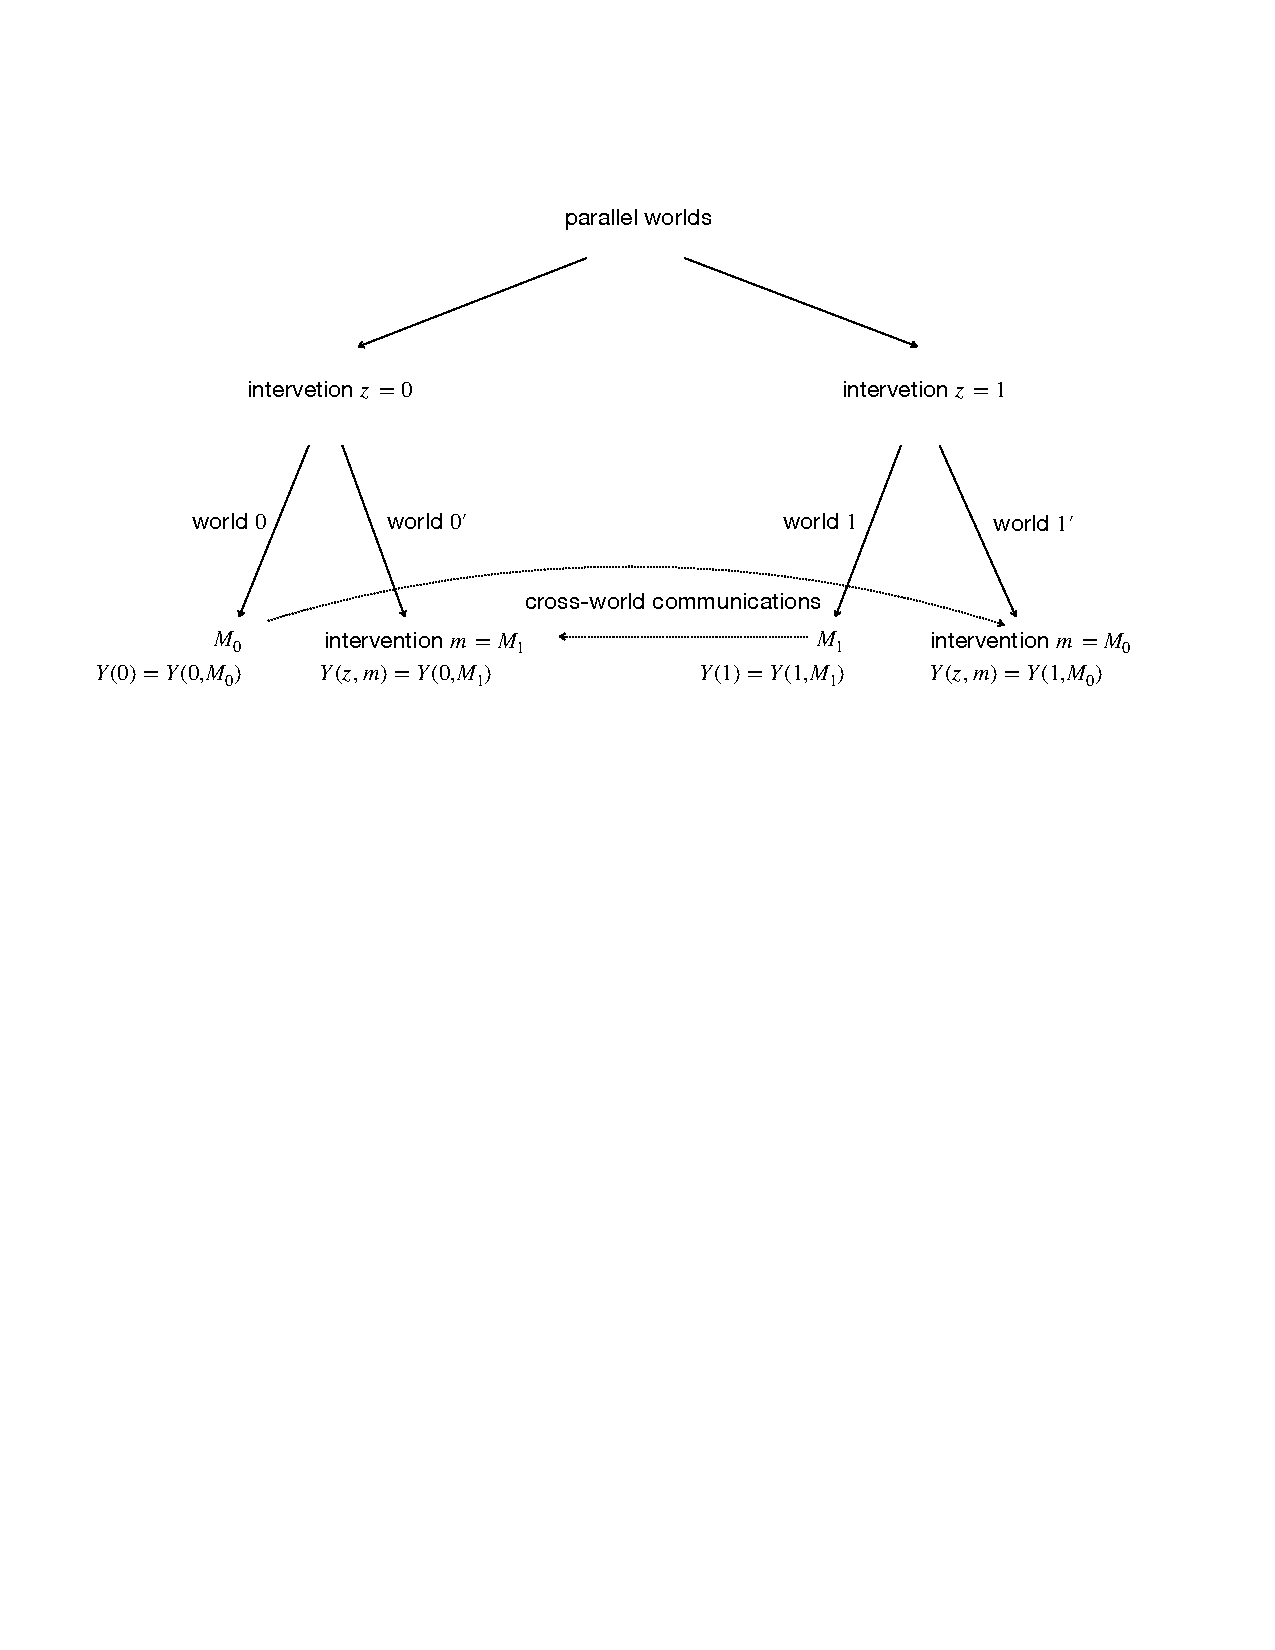
\includegraphics[width =  \textwidth]{figures/crossworld.pdf}
\caption{跨情境潜在结果 $Y(1,M_0)$ 与 $Y(0, M_1)$ 的概念示意图}\label{fg::crossworld}
\end{figure}




\section{中介效应计算公式}

\citet{Pearl::2001}的中介公式推导基于下述四重假设。前三重假设实质要求处理与中介均需在给定协变量条件下呈随机化分布。

\begin{assumption}
\label{assume::mediation1}
不存在处理与结果之间的混杂：
$$
Z\ind Y(z,m)\mid X
$$
对所有$z$与$m$成立。
\end{assumption}

\begin{assumption}
\label{assume::mediation2}
不存在中介与结果之间的混杂：
$$
M \ind Y(z,m) \mid (X, Z)
$$
对所有$z$与$m$成立。
\end{assumption}

假设\ref{assume::mediation1}与\ref{assume::mediation2}合称{\it 序贯可忽略性}，等价于给定$X$后$(Z, M)$联合随机化：
\begin{eqnarray}\label{eq::joint-randomization}
(Z, M) \ind Y(z,m)\mid X
\end{eqnarray}
对所有$z$与$m$成立。\eqref{eq::joint-randomization}的证明留作习题\ref{para::sr-jr}。 



\begin{assumption}
\label{assume::mediation3}
处理与中介间无混杂效应：
$$
Z \ind M(z) \mid X
$$ 
对所有可能值 $z$ 均成立。 
\end{assumption}

最后第四重假设涉及跨情境独立性： 

\begin{assumption}
\label{assume::mediation4}
不存在跨情境独立性：
$$
Y(z,m) \ind M(z') \mid X
$$ 
对所有可能值 $z,z'$ 与 $m$ 均成立。 
\end{assumption}


假设\ref{assume::mediation1}至\ref{assume::mediation3}很强，但至少在处理与中介均随机化的实验中成立。假设\ref{assume::mediation4}更强，没有物理实验能够保证它。$z\neq z'$时，任何实验都不能同时观测$Y(z,m)$与$ M(z') $，因此假设\ref{assume::mediation4}永远无法验证，具有根本的形而上学性质。 

下面给出假设\ref{assume::mediation1}至\ref{assume::mediation4}全部成立的例子。 

\begin{example}
\label{eg::mediation-assumptions}
给定$X$，生成
\begin{eqnarray*}
Z &=& 1\{  g_Z(X, \varepsilon_Z)  \geq 0 \} ,\\
M(z) &=& 1\{   g_M(X, z, \varepsilon_M)  \geq 0 \} ,\\
Y(z,m) &=& g_Y(X, z, m, \varepsilon_Y ),
\end{eqnarray*}
其中$z,m = 0,1$，
$
\varepsilon_Z, \varepsilon_M,
\varepsilon_Y 
$
是相互独立的随机误差。再由
\begin{eqnarray*}
M &=& M(Z) = 1\{   g_M(X, Z, \varepsilon_M)  \geq 0 \},\\
Y &=& Y(Z,M) = g_Y(X, Z, M, \varepsilon_Y ) . 
\end{eqnarray*}
生成$M$与$Y$的观测值。可验证，在该数据生成过程下，假设\ref{assume::mediation1}至\ref{assume::mediation4}成立。反之，若允许$  \varepsilon_M$与$\varepsilon_Y$分别变为$ \varepsilon_M(z)$和$\varepsilon_Y(z,m)$，假设\ref{assume::mediation1}至\ref{assume::mediation4}就可能不成立，详见习题\ref{para::mediation-assumptions-DGP}。
\end{example}



\citet{Pearl::2001}最终证明如下重要结论： 

\begin{theorem}
\label{thm::mediation}
在假设 \ref{assume::mediation1}--\ref{assume::mediation4} 条件下，成立
$$
E\{ Y(z, M_{z'})  \mid X=x \} =  \sum_m E(Y\mid Z=z, M=m, X=x) \pr(M =  m \mid Z=z', X=x)   
$$
从而可推导得
\begin{eqnarray*}
&&E\{ Y(z, M_{z'})   \}  \\
&=&  \sum_x E\{ Y(z, M_{z'})  \mid X=x \} \pr(X =  x )  \\
&=&  \sum_x \sum_m E(Y\mid Z=z, M=m, X=x) \pr(M =  m \mid Z=z', X=x)   \pr(X =  x ).
\end{eqnarray*}
\end{theorem}

 

定理\ref{thm::mediation}假定$M$与$X$均离散。对于一般的$M$与$X$，中介公式为
$$
E\{ Y(z, M_{z'}) \mid X=x  \} =   \int  E(Y\mid Z=z, M=m, X=x) f ( m \mid Z=z', X=x) \d m
$$
和
\begin{eqnarray*}
&&E\{ Y(z, M_{z'})   \}  \\
 &=& \int E\{ Y(z, M_{z'}) \mid X=x  \}   f  (x) \d x  \\
 &=& \int \int  E(Y\mid Z=z, M=m, X=x) f ( m \mid Z=z', X=x)     f  (x) \d m \d x   . 
\end{eqnarray*}
由定理\ref{thm::mediation}可见，嵌套潜在结果均值的识别，依赖给定处理、中介和协变量后的结果条件均值，以及给定处理与协变量后的中介条件分布。若涉及跨世界干预，就需要在不同处理水平上分别计算上述条件量。 

若放弃前述跨情境独立性假设，直接效应与间接效应定义可相应调整，此时仍可得相同计算公式。详细论证见习题 \ref{problem::no-crossworld-modification}。  

下面给出该定理的证明： 
 

\begin{myproof}{定理}{\ref{thm::mediation}}由塔性质，$E\{ Y(z, M_{z'})   \}  =  E[ E\{ Y(z, M_{z'})  \mid X\}  ]$，所以只需证明$E\{ Y(z, M_{z'})  \mid X=x\}$的公式。从全概率公式出发，
\begin{eqnarray*}
&& E\{ Y(z, M_{z'})  \mid X=x\}  \\
&=& 
\sum_m E\{ Y(z, M_{z'})  \mid  M_{z'} = m, X=x\} \pr(  M_{z'} = m\mid X=x) \\
&=&
\sum_m E\{ Y(z, m)  \mid  M_{z'} = m, X=x\} \pr(  M_{z'} = m\mid X=x) \\ 
&=& 
\sum_m \underbrace{ E\{ Y(z, m)  \mid    X=x\} }_{\text{Assumption }\ref{assume::mediation4} } 
\underbrace{ \pr(  M  = m\mid Z=z' , X=x) }_{\text{Assumption }\ref{assume::mediation3} } \\ 
&=&
\sum_m \underbrace{E( Y  \mid  Z=z, M=m,   X=x)}_{ \text{Assumptions }\ref{assume::mediation1}\text{ and }\ref{assume::mediation2} } 
\pr(  M  = m\mid Z=z' , X=x) .
\end{eqnarray*}
%Averaging over $X$, we obtain the mediation formula. 
\end{myproof}


上述证明在数学上很简单，也说明了假设\ref{assume::mediation1}至\ref{assume::mediation4}各自的必要作用。 


给定$X=x,$，由全概率公式，$Y(1, M_1)$与$Y(0, M_0)$的中介公式分别简化为
\begin{eqnarray*}
&& E\{  Y(1, M_1)\mid X=x \} \\ 
&=& \sum_m E( Y  \mid  Z=1, M=m,   X=x) \pr(M=m \mid Z=1, X=x)\\
&=& E( Y  \mid  Z=1 ,  X=x)
\end{eqnarray*}
和
\begin{eqnarray*}
&&E\{  Y(0, M_0)\mid X=x \}  \\
&=& \sum_m E( Y  \mid  Z=0, M=m,   X=x) \pr(M=m \mid Z=0, X=x)\\
&=& E( Y  \mid  Z=0 ,  X=x)
\end{eqnarray*}
$Y(1, M_0)$的中介公式简化为
\begin{eqnarray*}
&&E\{  Y(1, M_0)\mid X=x \}  \\
&=&  \sum_m E( Y  \mid  Z=1, M=m,   X=x) \pr(M=m \mid Z=0, X=x),
\end{eqnarray*}
其中结果条件期望取$Z=1$，而中介条件分布取$Z=0$。由此得到自然直接效应和间接效应的识别公式。

\begin{corollary}
\label{corollary::mediation-nde-nie}
在假设 \ref{assume::mediation1}--\ref{assume::mediation4} 条件下，条件自然直接效应与间接效应定义为：
\begin{eqnarray*}
\NDE(x) &=& E\{ Y(1, M_0) - Y(0, M_0) \mid X=x \} \\
&=& \sum_m \{ E( Y  \mid  Z=1, M=m,   X=x) - E( Y  \mid  Z=0, M=m,   X=x) \} \\
&& \qquad  \times \pr(M=m \mid Z=0, X=x)
\end{eqnarray*}
以及
\begin{eqnarray*}
\NIE(x) &=& E\{ Y(1, M_1) - Y(1, M_0) \mid X=x \} \\
&=& \sum_m   E( Y  \mid  Z=1, M=m,   X=x)\\
&&  \qquad  \times  \{ \pr(M=m \mid Z=1, X=x) -  \pr(M=m \mid Z=0, X=x) \};
\end{eqnarray*}
无条件效应值可通过全期望公式计算：$\NDE = \sum_ x \NDE(x) \pr(X=x)$ 与 $\NIE = \sum_ x \NIE(x) \pr(X=x)$。
\end{corollary}





作为特例，若$M$为二元变量，$\NIE$公式简化为下面的乘积形式。


\begin{corollary}
\label{corollary::mediation-binary-M}
在假设 \ref{assume::mediation1}--\ref{assume::mediation4} 条件下，若中介 $M$ 为二元变量，则
$$
\NIE(x)  =      \tau_{Z\rightarrow M} (x) \tau_{M\rightarrow Y} (1,x)
$$
且
$
\NIE = E\{  \NIE(X)   \},
$
其中
$$
\tau_{Z\rightarrow M}(x) =  \pr(M=1 \mid Z=1, X=x) -  \pr(M=1 \mid Z=0, X=x) . 
$$
以及
$$
\tau_{M\rightarrow Y} (z,x) = E( Y  \mid  Z=z, M=1,   X=x) - E( Y  \mid  Z=z, M=0,   X=x)
$$
\end{corollary}

推论\ref{corollary::mediation-binary-M}的证明留作习题\ref{para::nie-binary-m}。推论\ref{corollary::mediation-binary-M}给出二元$M$下的简单公式：若给定$X$后$Z$随机化，可将$\tau_{Z\rightarrow M}(x) $视为$Z$对$M$的条件平均因果效应；若给定$(X,Z)$后$M$随机化，可将$\tau_{M\rightarrow Y} (z,x) $视为$M$对$Y$的条件平均因果效应。条件自然间接效应等于二者之积，符合间接作用由$Z$到$M$、再由$M$到$Y$传递的直观理解。 


\section{线性模型下的中介效应计算}


前述定理 \ref{thm::mediation} 给出非参数框架下的计算方案。基于此可推导各类模型下的中介效应公式。下文详述在线性假设下著名的Baron-Kenny方法。\citet{vanderweele2015explanation}亦给出了多种常用模型下的相应公式。其他模型情形留待 \ref{chapter::mediation-problmes} 章探讨。 

\subsection{Baron-Kenny方法}


\begin{figure}[ht]
\centering
$$
\begin{xy}
\xymatrix{
&  & X \ar[ddll] \ar[dd]^{\beta_2} \ar[ddrr]^{\theta_4} \\
&&\\
Z \ar[rr]^{\beta_1} \ar@/_2.8pc/[rrrr]_{\theta_1} & & M\ar[rr]^{\theta_2} & & Y & \text{indirect effect: } \beta_1\theta_2 \\
&&&&& \text{  direct effect: } \theta_1 }
\end{xy}
$$
\caption{线性模型下的Baron-Kenny中介分析示意图}\label{fg::mediationDAG-BK}
\end{figure}

Baron--Kenny 方法假定，在给定处理与协变量后，中介和结果满足以下线性模型。

\begin{assumption}
[Baron-Kenny方法所用线性模型]
\label{assume::mediation-bk-model}
中介与结果均服从线性模型：
$$
\left\{\begin{array}{rcl}
E(M \mid Z, X) &=&  \beta_0 + \beta_1 Z + \beta_2\tran X, \\
E(Y\mid Z,M,X) &=& \theta_0 + \theta_1 Z + \theta_2 M + \theta_4\tran X.
\end{array}\right.
$$
\end{assumption}


 
在此模型下中介效应可简化为系数乘积形式： 

\begin{corollary}
[Baron-Kenny中介效应公式]
\label{corollary::bk-formulas}
在假设 \ref{assume::mediation1}--\ref{assume::mediation4} 与 \ref{assume::mediation-bk-model} 条件下，我们有 
$$
\NDE = \theta_1
,\quad 
\NIE = \theta_2 \beta_1 .
$$
\end{corollary}


从图\ref{fg::mediationDAG-BK}看，推论\ref{corollary::bk-formulas}的公式很直观：直接效应等于路径$Z\rightarrow Y$上的系数，间接效应等于路径$Z\rightarrow M\rightarrow Y$上的系数之积。下面基于定理\ref{thm::mediation}证明。 


\begin{myproof}{推论}{\ref{corollary::bk-formulas}}条件自然直接效应为
$$
\NDE(x)  
= \sum_m  \theta_1  \pr(M=m \mid Z=0, X=x) = \theta_1
$$
条件自然间接效应为
\begin{eqnarray*}
\NIE(x) &=&  \sum_m  (\theta_0 + \theta_1  + \theta_2 m + \theta_4\tran x )\\
&&  \qquad  \times  \{ \pr(M=m \mid Z=1, X=x) -  \pr(M=m \mid Z=0, X=x) \} \\
&=& \theta_2 \{ E(M=m \mid Z=1, X=x) -  E(M=m \mid Z=0, X=x) \} \\
&=&  \theta_2 \beta_1 ,
\end{eqnarray*}
二者均不依赖$x$，因此也是无条件自然直接效应与间接效应的公式。
\end{myproof}


 
使用OLS估计上述系数后可得：
$$
\hat{\NDE} = \hat{\theta}_1,\qquad
\hat{\NIE} = \hat{\theta}_2 \hat{\beta}_1,
$$
此即Baron-Kenny方法\citep{Judd::1981, baron1986moderator}的核心算法，虽其渊源可追溯至早期研究\citep[e.g.,][]{hyman1955survey, alwin1975decomposition, Judd::1981, sobel1982asymptotic}。


标准软件包报告 OLS 得到的$\hat{\NDE}$标准误。\citet{sobel1982asymptotic, sobel1986some}则用 delta 方法求出$\hat{\NIE}$的标准误。 
%Based on the heuristics:
%\begin{eqnarray*}
%\hat{\theta}_2  \hat{\beta}_1 -  \theta_2 \beta_1
%&=& \hat{\theta}_2  \hat{\beta}_1 -  \theta_2 \hat{\beta}_1 +   \theta_2 \hat{\beta}_1  -  \theta_2 \beta_1 \\
%&=&  (\hat{\theta}_2 -  \theta_2 )  \hat{\beta}_1 + \theta_2 (\hat{\beta}_1 - \beta_1 ) \\
%&\approx& (\hat{\theta}_2 -  \theta_2 )   \beta_1 + \theta_2 (\hat{\beta}_1 - \beta_1 )
%\end{eqnarray*}
%and the independence of $\hat{\theta}_2 $ and $ \hat{\beta}_1$, 
由例\ref{example::asymptotic-normal-product}的公式，$\hat{\theta}_2  \hat{\beta}_1 $的渐近方差为
$
\var(\hat{\theta}_2)  \beta_1^2 + \theta_2^2 \var(\hat{\beta}_1) .
$
因此，估计方差为
$$
\hat{\var}(\hat{\theta}_2)  \hat{\beta}_1^2 + \hat{\theta}_2^2 \hat{\var}(\hat{\beta}_1) .
$$
利用$\hat{\theta}_2 \hat{\beta}_1$及上述方差估计检验$\NIE$为零的零假设，在中介分析文献中称为{\it Sobel 检验}。 


 


\subsection{实例演示}\label{section::BK-jobs}

以下代码可方便地实现 Baron--Kenny 方法。 

 \begin{lstlisting}
library("car")
BKmediation = function(Z, M, Y, X)
{
  ## two regressions and coefficients
  mediator.reg   = lm(M ~ Z + X)
  mediator.Zcoef = mediator.reg$coef[2]
  mediator.Zse   = sqrt(hccm(mediator.reg)[2, 2])
  
  outcome.reg    = lm(Y ~ Z + M + X)
  outcome.Zcoef  = outcome.reg$coef[2]
  outcome.Zse    = sqrt(hccm(outcome.reg)[2, 2])
  outcome.Mcoef  = outcome.reg$coef[3]
  outcome.Mse    = sqrt(hccm(outcome.reg)[3, 3])
  
  ## Baron-Kenny point estimates
  NDE = outcome.Zcoef
  NIE = outcome.Mcoef*mediator.Zcoef
  
  ## Sobel's variance estimate based the delta method
  NDE.se = outcome.Zse
  NIE.se = sqrt(outcome.Mse^2*mediator.Zcoef^2 + 
                  outcome.Mcoef^2*mediator.Zse^2)
  
  res = matrix(c(NDE, NIE, 
                 NDE.se, NIE.se,
                 NDE/NDE.se, NIE/NIE.se), 
               2, 3)
  rownames(res) = c("NDE", "NIE")
  colnames(res) = c("est", "se", "t")
  
  res
}
 \end{lstlisting}
 
 
 以前文 \ref{eg::mediation-jobs} 的JOBS数据集为例得到如下结果：
 
 \begin{lstlisting}
> jobsdata = read.csv("jobsdata.csv")
> Z = jobsdata$treat
> M = jobsdata$job_seek
> Y = jobsdata$depress2
> getX     = lm(treat ~ econ_hard + depress1 + 
+                 sex + age + occp + marital + 
+                 nonwhite + educ + income,
+               data = jobsdata)
> X = model.matrix(getX)[, -1]
> res = BKmediation(Z, M, Y, X)
> round(res, 3)
       est    se      t
NDE -0.037 0.042 -0.885
NIE -0.014 0.009 -1.528
\end{lstlisting}

结果显示直接与间接效应估计值均为负值，但均不显著。 



\section{敏感性分析}


中介分析建立在多种强假设基础之上，其中核心之一是处理-中介-结果间不存在不可观测混杂因素。目前已有多种敏感性分析工具；\citet{ding2016sharp}提出基于Cornfield方法的敏感性界限；\citet{zhang2022interpretable}则针对Baron-Kenny框架提出特定分析方案。这些内容已超出本书范围。  





 

\section{作业习题}\label{chapter::mediation-problmes}



\paragraph{\citet{Robins::1992}关于嵌套潜在结果的单元分类}\label{hw::robins1992-latentgroups}


假设$(Z, M, Y)$均为二元变量。根据
$$
M(1), M(0),  Y(1, M_1), Y(1, M_0), Y(0, M_1), Y(0, M_0) ,
$$
的联合取值，共有多少类单位？

若假定$Z$对$M$的单调性，即
$$
M(1) \geq  M(0),
$$
则有多少类单位？

若进一步假定$Z$与$M$对$Y$具有单调性，即对所有$z$和$m$有
$$
Y(1, m) \geq Y(0, m),  \quad Y(z, 1) \geq Y(z, 0)
$$
则有多少类单位？


\paragraph{逐次随机化与联合随机化}\label{para::sr-jr}

请证明式 \eqref{eq::joint-randomization} 与假设 \ref{assume::mediation1} 和 \ref{assume::mediation2} 等价。 


\paragraph{验证中介分析假设条件}\label{para::mediation-assumptions-DGP}

证明，在例\ref{eg::mediation-assumptions}的数据生成过程中，假设\ref{assume::mediation1}至\ref{assume::mediation4}成立。并说明若允许$  \varepsilon_M$和$\varepsilon_Y$分别变为$ \varepsilon_M(z)$与$\varepsilon_Y(z,m)$，假设\ref{assume::mediation1}至\ref{assume::mediation4}就可能失败。 
 
 \paragraph{中介效应的替代定义方式}\label{para::alternative-si}



\citet{Imai::2010}采用不同假设推导相应计算式： 

\begin{assumption}
\label{assume::mediation-imai}
满足
$$
\{Y(z, m), M(z') \} \ind  Z\mid X
$$
以及
$$
Y(z, m) \ind M(z' ) \mid (Z=z' , X)
$$
对所有 $z, z', m$ 均成立。
\end{assumption}


\begin{theorem}
\label{thm::mediation-imai}
在假设\ref{assume::mediation-imai}下，定理\ref{thm::mediation}的中介公式成立。 
\end{theorem}


证明定理 \ref{thm::mediation-imai}。 



\paragraph{差异法与乘积法的等价性}\label{hw::difference=product}


正文先进行 OLS 拟合
$$
\left\{\begin{array}{rcl}
\hat M_i &=&  \hat\beta_0 + \hat\beta_1 Z_i + \hat\beta_2\tran X_i, \\
\hat Y_i &=&\hat \theta_0 + \hat\theta_1 Z_i +\hat \theta_2 M_i + \hat\theta_4\tran X_i.
\end{array}\right.
$$
以乘积$\hat \theta_2 \hat\beta_1 $估计自然间接效应，称为乘积法。 

也可先进行 OLS 拟合
$$
\left\{\begin{array}{rcl}
\hat Y_i &=&  \hat\alpha_0 + \hat\alpha_1 Z_i + \hat\alpha_1 \tran X_i, \\
\hat Y_i &=&\hat \theta_0 + \hat\theta_1 Z_i +\hat \theta_2 M_i + \hat\theta_4\tran X_i.
\end{array}\right.
$$
用差值$\hat\alpha_1 -  \hat\theta_1$估计自然间接效应，称为差分法。 

证明 $\hat\alpha_1 -  \hat\theta_1 = \hat \theta_2 \hat\beta_1 .$


注：回顾习题\ref{hw::cochran+ovb}中的 Cochran 公式。 



\paragraph{二元中介下的自然间接效应}\label{para::nie-binary-m}

请证明推论 \ref{corollary::mediation-binary-M} 所陈述内容。 


\paragraph{处理与结果存在交互作用时的中介效应}\label{para::interaction}
\citet{vanderweele2015explanation}建议采用如下线性模型：
$$
\left\{\begin{array}{rcl}
E(M \mid Z, X) &=&  \beta_0 + \beta_1 Z + \beta_2\tran X, \\
E(Y\mid Z,M,X) &=& \theta_0 + \theta_1 Z + \theta_2 M + \theta_3 ZM + \theta_4\tran X,
\end{array}\right.
$$
其中结果模型包含处理与中介的交互项。 


在这些线性模型下，证明
$$
\NDE = \theta_1 + \theta_3\{ \beta_0 + \beta_2\tran E(X)\}, \qquad 
\NIE = (\theta_2 + \theta_3 ) \beta_1. 
$$
如何用独立同分布数据估计$\NDE$与$\NIE$？

注：考虑$Z$与$M$均为二元变量的简单情形。在线性模型下，$Z$对$M$的平均因果效应为$\beta_1$，$M$对$Y$的平均因果效应为$\theta_2 + \theta_3 E(Z)$。因此，两者都为正时，自然间接效应仍可能为负。例如：
$$
\beta_1 = 1,\quad \theta_2 = 1, \quad  \theta_3= -1.5, \quad E(Z) = 0.5.
$$
这有些反直觉，可称为{\it 中介悖论}。\citet{chen2007criteria}报告了相关的{\it 替代终点悖论}，也称{\it 中间变量悖论}。



\paragraph{放弃跨情境独立性假设后的定义调整}\label{para::continM-binaryY}


考虑中介的以下正态线性模型，以及二元结果的逻辑回归模型：
$$
\left\{\begin{array}{rcl}
M \mid Z, X &\sim &  \textsc{N}(\beta_0 + \beta_1 Z + \beta_2\tran X, \sigma_M^2), \\
\logit \{ \pr(Y = 1 \mid Z,M,X ) \} &=& \theta_0 + \theta_1 Z + \theta_2 M +   \theta_4\tran X,
\end{array}\right.
$$
其中$\logit (w)  = \log\{ w/(1-w) \} $，其反函数为$\expit(w) = (1 + e^{-w})^{-1}.$。用模型参数和$X$的分布表示$\NDE$与$\NIE$。如何用独立同分布数据估计$\NDE$和$\NIE$？




\paragraph{二元中介与连续结果的中介分析}\label{para::logit-binary-m}
考虑二元中介的逻辑回归模型与结果的线性模型：
$$
\left\{\begin{array}{rcl}
\logit\{ \pr(M  = 1\mid Z, X) \}&=&  \beta_0 + \beta_1 Z + \beta_2\tran X, \\
E(Y\mid Z,M,X) &=& \theta_0 + \theta_1 Z + \theta_2 M +   \theta_4\tran X . 
\end{array}\right.
$$
%where $\logit (w)  = \log\{ w/(1-w) \} $ with inverse $\expit(w) = (1 + e^{-w})^{-1}.$


在这些模型下，证明
$$
\NDE = \theta_1  ,\qquad
\NIE = \theta_2 E \left\{  \expit(\beta_0 + \beta_1  + \beta_2\tran X)
-  \expit(\beta_0   + \beta_2\tran X)  \right\}. 
$$
如何用独立同分布数据估计$\NDE$与$\NIE$？






\paragraph{主分层法与中介分析的关系}
\label{para::mediation-binaryMY}

考虑二元中介与结果的以下逻辑回归模型：
$$
\left\{\begin{array}{rcl}
\logit\{ \pr(M  = 1\mid Z, X) \}&=&  \beta_0 + \beta_1 Z + \beta_2\tran X, \\
\logit \{ \pr(Y = 1 \mid Z,M,X ) \} &=& \theta_0 + \theta_1 Z + \theta_2 M +   \theta_4\tran X.
\end{array}\right.
$$
用模型参数及$X$的分布表示$\NDE$与$\NIE$。如何用独立同分布数据估计$\NDE$和$\NIE$？



  
\paragraph{修改定义以去掉跨世界独立性假设}\label{problem::no-crossworld-modification}


定义
$$
Y(z, F_{M_{z'}\mid X}) = \int Y(z,m) f(M_{z'} = m\mid X) \d m
$$
作为处理为$z$、中介值从$M_{z'}\mid X$分布随机抽取时的潜在结果。若$M$离散，定义简化为
$$
Y(z, F_{M_{z'}\mid X}) =\sum_m Y(z,m) \pr(M_{z'} = m\mid X).
$$
$Y(z,M_{z'})$与$Y(z, F_{M_{z'}\mid X}) $的关键区别是：$M_{z'}$为同一单位的潜在中介，而$F_{M_{z'}\mid X}$对应整个总体中潜在中介的条件分布，按该分布随机抽取中介值。定义自然直接效应与间接效应为
$$
\NDE = E\{Y(1, F_{M_{0}\mid X})  - Y(0, F_{M_{0}\mid X})   \},\quad
\NIE  =  E\{Y(1, F_{M_{1}\mid X})  - Y(1, F_{M_{0}\mid X})   \}.
$$


证明：在假设\ref{assume::mediation1}至\ref{assume::mediation3}下，$\NDE$与$\NIE$的识别公式仍与正文相同。 



注：修改嵌套潜在结果的定义后，可以放松较强的跨世界独立性假设，但也削弱了自然直接效应与间接效应的原有解释。进一步讨论见\citet{vanderweele2015explanation}；\citet{vanderweele2017mediation}将其应用于处理与中介均随时间变化的更复杂情形。

  
  
\paragraph{主分层与中介分析的联系}

\citet{vanderweele2008simple}与\citet{forastiere2018principal}分别评述了主分层法与中介分析的联系与区别。 
    
       
\chapter{受控直接效应}
 \label{chapter::cde}


第\ref{chapter::mediation}章中所述的中介分析方法是基于嵌套潜在结果来构建的；从根本上而言，某些嵌套潜在结果在任何实际实验中都无法被观测到。如果我们遵循第\ref{sec::popper-science}章中介绍的波普尔科学哲学观点，那么我们应当仅用实验中可观测的量来定义因果参数。本章将探讨一种处理带有中介变量情况下的因果推断的替代方法：在这种观点下，我们只能定义直接效应，却无法定义间接效应。 





\section{受控直接效应的定义}


我们将$Z$与$M$视作两个可人为干预的处理因素，并定义当$z=0,1$且$m\in \mathcal{M}$时的潜在结果$Y(z,m)$。基于这些潜在结果，我们可定义下文中的{\it 受控直接效应}(CDE)。

\begin{definition}
[CDE]
定义
$$
\CDE (m)  = E\{  Y(1,m)  - Y(0,m)\}.
$$
\end{definition}
  
 
根据定义，$\CDE (m) $是在将中间变量固定为$m$时，处理的平均因果效应。参数$\CDE(m)$可以刻画将中介变量固定为$m$时的直接效应，但这一设定无法刻画间接效应。特别地，参数
$
E\{  Y(z,1) - Y(z,0)\}
$
仅衡量将处理固定为$z.$时中介变量对结果的效应，不能将其视为有意义的间接效应定义。 



\section{受控直接效应的识别与估计}


为了识别$\CDE(m)$，我们需要以下假设：即给定$X$时，$Z$与$M$均受到随机化处理。 


\begin{assumption}\label{assume::si-cde}
序列无偏性要求满足
$$
Z\ind Y(z,m) \mid X, \quad M \ind  Y(z,m) \mid (Z,X)
$$
或等价地（参见问题\ref{para::sr-jr}），
$$
(Z,M) \ind  Y(z,m) \mid X.
$$
\end{assumption}

下面着重讨论$Z$和$M$均为二元变量的情形。从数学上看，可以将其视为具有四个处理水平
$$
(z,m) \in \{  (0,0), (0,1), (1,0), (1,1) \} .
$$
的观察性研究。以下定理推广了二元处理观察性研究的结论，分别通过结果回归、IPW 和双重稳健估计识别
$$
\mu_{zm} = E\{  Y(z,m) \}
$$ 


定义
$$ 
\mu_{zm}(x) = E(Y\mid Z=z,M=m, X=x) 
$$
为在给定处理、中介变量以及协变量条件下的结果均值；定义
\begin{eqnarray*}
e_{zm}(x)  &=&  \pr(Z=z,M=m\mid X=x)  \\
&=& \pr(Z=z\mid X=x) \pr( M=m\mid Z=z, X=x)
\end{eqnarray*} 
为给定协变量时$Z$与$M$同时出现的概率。 

\begin{theorem}
\label{thm::cde-identification}
在假设\ref{assume::si-cde}成立的前提下，我们有
$$
\mu_{zm} = E\{  \mu_{zm}(X) \}
= E \left\{   \frac{I(Z=z, M=m) Y}{  e_{zm}(X)  }  \right\} .
$$
此外，若以$e_{zm}(X, \alpha) $与$\mu_{zm}(X, \beta) $分别作为$e_{zm}(X) $和$\mu_{zm}(X) $的拟合模型，则可得到双重稳健估计式：
$$
\mu_{zm}^{\textup{dr}}  = E\{  \mu_{zm}(X, \beta) \} + E \left[   \frac{I(Z=z, M=m) \{ Y - \mu_{zm}(X, \beta)  \}}{  e_{zm}(X, \alpha)  }  \right],
$$
只要满足$e_{zm}(X, \alpha) = e_{zm}(X)$或$\mu_{zm}(X, \beta)  = \mu_{zm}(X)$中的任一条件，该估计值即等于$\mu_{zm} $。 
\end{theorem}



定理\ref{thm::cde-identification}的证明与标准无混杂观察性研究中的证明类似，习题\ref{para::obs-multi-valued-Z}给出了一般结论。根据结果均值模型，可得到$\mu_{zm}(x)$的估计$\hat{\mu}_{zm}(x) $；根据处理模型，可得到$\pr(Z=z\mid X = x)$的估计$\hat{e}_z(x)$；根据中间变量模型，可得到$\pr(M=m\mid Z=z, X=x)$的估计$\hat{e}_m(z,x)$。于是可用结果回归
$$
\hat{\mu}_{zm}^\text{reg} = n^{-1} \sumn  \hat{\mu}_{zm}(X_i),
$$
、IPW
\begin{eqnarray*}
\hat{\mu}_{zm}^\text{ht} &=& n^{-1}\sumn  \frac{  I(Z_i=z, M_i=m) Y_i  }{  \hat{e}_z(X_i)  \hat{e}_m(z,X_i)  } , \\
\hat{\mu}_{zm}^\text{haj} &=&  \sumn  \frac{  I(Z_i=z, M_i=m) Y_i  }{  \hat{e}_z(X_i)  \hat{e}_m(z,X_i)  } \Big /  \sumn  \frac{  I(Z_i=z, M_i=m)    }{  \hat{e}_z(X_i)  \hat{e}_m(z,X_i)  }, 
\end{eqnarray*}
或增广 IPW
$$
\hat{\mu}_{zm}^\text{dr} = \hat{\mu}_{zm}^\text{reg}  +  n^{-1} \sumn  \frac{  I(Z_i=z, M_i=m) \{ Y_i - \hat{\mu}_{zm}(X_i)\}   }{  \hat{e}_z(X_i)  \hat{e}_m(z,X_i)  } .
$$
估计$\mu_{zm} $。进一步用$\hat{\mu}_{1m}^* - \hat{\mu}_{0m}^*\ (*=\text{reg}, \text{ht}, \text{haj}, \text{dr} )$估计$\CDE(m)$，并用自助法近似其标准误。 




若我们假定结果为线性模型，则受控直接效应便简化为处理变量的系数。例\ref{eg::cde-linear}将详细说明这一过程。 
\begin{example}
\label{eg::cde-linear}
在假设\ref{assume::si-cde}成立且结果模型为线性的条件下，
$$
E(Y\mid Z,M,X) = \theta_0 + \theta_1 Z + \theta_2 M +   \theta_4\tran X,
$$
可以证明
$
\CDE(m) 
$
其值等同于系数$ \theta_1$，这与Baron-Kenny法中定义的自然直接效应相一致。证明过程留作问题\ref{problem::cde-linear}供读者自行验证。 
\end{example}







\section{讨论}

受控直接效应的定义方式不涉及任何嵌套或预先假设的潜在反事实结果，其识别过程也无需“跨世界反事实独立性”假设。参数$\CDE(m)$可反映中介变量保持为$m$时处理的直接效应；然而它无法反映间接效应。表\ref{table::causal-intermediate-frameworks}总结了各类涉及中介变量的因果分析框架。 
 
\begin{table}
\centering 
\caption{涉及中介变量的各类因果分析框架}\label{table::causal-intermediate-frameworks}
\begin{tabular}{cccc}
\hline 
章节 & 框架 & 直接效应 & 间接效应   \\
\hline 
\ref{chapter::principal-stratification} & 主分层法 & $\tau(1,1),\ \tau(0,0)$ & ?  \\
\ref{chapter::mediation} & 中介分析法 & $\NDE$ & $\NIE$  \\
\ref{chapter::cde}& 控制直接效应 & $\CDE(m)$ & ?  \\
\hline 
\end{tabular}
\end{table} 
 
中介分析法能将总效应分解为自然直接效应与间接效应，但它需要嵌套潜在结果及跨世界独立性假设；主分层法与受控直接效应法虽无法定义间接效应，却无需上述假设。另外，主分层法并不要求$M$一定位于从处理到结果的因果路径上；不过其识别与估计过程涉及混合分布的分离，这在统计学上属难度较高的任务。 



  
  \section{作业习题}

\paragraph{$\CDE$与$\NDE$}\label{problem::cde-nde}

试证明：在“跨世界独立性”假设成立时，即对所有$z,z'$与$m$均有
$
Y(z,m) \ind M(z') \mid X
$
此时条件受控直接效应$\CDE(m\mid x) = E\{  Y(1,m)  - Y(0,m)\mid X=x\}$与条件自然直接效应$\NDE(x) = E\{   Y(1,M_0) - Y(0, M_0) \mid X=x  \}$满足如下关系：
$$
\NDE(x) = \sum_m \CDE(m\mid x) \pr(M_0 = m\mid X=x)
$$
此处$M$为离散型变量。若上述独立性假设不成立，该关系是否仍普遍成立？ 
  
  
  
  \paragraph{含多值处理的观察研究}\label{para::obs-multi-valued-Z}
  
定理\ref{thm::cde-identification}其实是如下关于“含多值处理的无混杂观察研究”一般结论的一个特例\citep{imai2004causal, cattaneo2010efficient}。下文给出该一般问题的描述及相关定理。 



考虑一项观察性研究，其中处理$Z \in \{ 1, \ldots, K \}$有多个取值，协变量为$X$，结果为$Y$。单位$i$有$K$个潜在结果$Y_i(1), \ldots, Y_i(K)$，分别对应$K$个处理水平。一般地，可以通过潜在结果的对比定义因果效应：
$$
\tau_C  = \sum_{k=1}^K C_k   E\{  Y(k) \}
$$
其中$  \sum_{k=1}^K C_k  = 0$。最常用的两两比较为
$$
\tau_{k,k'} = E\{   Y(k) - Y(k') \}.
$$
因此，关键是在以下可忽略性和重叠性假设下，利用$(Z_i,  X_i, Y_i)_{i=1}^n$的独立同分布数据识别并估计潜在结果的均值$\mu_k  =  E\{  Y(k) \}$。



\begin{assumption}
\label{assume::ignorability-multi-valued-Z}
$Z\ind \{ Y (1), \ldots, Y (K) \} \mid X$，且对于$k=1,\ldots, K.$有$\pr(Z = k \mid X) > 0$。
\end{assumption}



定义广义倾向得分
$$
e_k(X) = \pr(Z = k \mid X), 
$$
以及条件结果均值
$$
\mu_k(X) = E(   Y \mid Z=k,  X )
$$
其中$k=1, \ldots, K.$。有如下定理。

\begin{theorem}
\label{thm::treatment-multi-valued-Z}
在假设\ref{assume::ignorability-multi-valued-Z}成立的前提下，有
$$
\mu_{k} = E\{  \mu_{k}(X) \}
= E \left\{   \frac{I(Z = k) Y}{  e_{k}(X)  }  \right\} .
$$
另外，若以$e_{k}(X, \alpha) $与$\mu_{k}(X, \beta) $作为$e_{k}(X) $与$\mu_{k}(X) $的拟合模型，可得双重稳健估计式：
$$
\mu_{k}^{\textup{dr}}  = E\{  \mu_{k}(X, \beta) \} + E \left[   \frac{I(Z=k) \{ Y - \mu_{k}(X, \beta)  \}}{  e_{k}(X, \alpha)  }  \right],
$$
当满足$e_{k}(X, \alpha) = e_{k}(X)$或$\mu_{k}(X, \beta)  = \mu_{k}(X)$时，此估计值即等于$\mu_{k} $。 
\end{theorem}


请证明定理\ref{thm::treatment-multi-valued-Z}。


注：若将定理\ref{thm::cde-identification}中的$(Z,M)$视为具有四个水平的处理，则定理\ref{thm::cde-identification}就是定理\ref{thm::treatment-multi-valued-Z}的特例。$  \CDE (m) $是$\tau_C $的特例。 


  
  \paragraph{线性结果模型下的$\CDE$}\label{problem::cde-linear}
  
  试证明：在假设\ref{assume::si-cde}成立情况下，若满足
$E(Y\mid Z, M, X ) = \theta_0 + \theta_1 Z + \theta_2 M +   \theta_4\tran X$，
则对所有$m$均有
$$
  \CDE (m) = \theta_1
  $$
；若满足
$E(Y\mid Z, M, X ) = \theta_0 + \theta_1 Z + \theta_2 M + \theta_3 ZM +    \theta_4\tran X$，
则
$$
\CDE(m) =   \theta_1 + \theta_3 m. 
  $$
  
  
    \paragraph{逻辑回归结果模型下的$\CDE$}\label{problem::cde-logit}
  
  试证明：对于二值结果变量，在假设\ref{assume::si-cde}成立前提下，若
$$
  \logit \{ \pr(Y = 1\mid Z, M, X ) \} = \theta_0 + \theta_1 Z + \theta_2 M +   \theta_4\tran X ,
  $$ 
则
$$
  \CDE (m) = E\{ \expit( \theta_0 + \theta_1  + \theta_2 m +   \theta_4\tran X ) - \expit( \theta_0    + \theta_2 m +   \theta_4\tran X ) \} ; 
  $$
若
$$
  \logit \{ \pr(Y = 1\mid Z, M, X ) \} = \theta_0 + \theta_1 Z + \theta_2 M + \theta_3 ZM +    \theta_4\tran X,
  $$ 
则
$$
\CDE(m) =  E\{ \expit( \theta_0 + \theta_1  + \theta_2 m  +\theta_3 m +   \theta_4\tran X ) - \expit( \theta_0    + \theta_2 m +   \theta_4\tran X ) \}.
  $$
  
  
  
  \paragraph{推荐阅读} 

\citet{nguyen2020clarifying}对第\ref{chapter::mediation}章与第\ref{chapter::cde}章的相关内容进行了清晰易懂的综述。 

   
       
\chapter{时变处理与混杂因素}
 \label{chapter::timevarying}
 

在生物医学与社会科学领域，涉及随时间变化的处理方式的研究十分常见。詹姆斯·罗宾斯大力推动了生物统计学领域的相关研究。

一个典型的例子是：HIV感染者可能会随时间变化而间断性地服用叠氮胸苷这种抗逆转录病毒药物\citep{robins2000marginal, hernan2000marginal}。类似的问题也存在于其他领域。在教育领域，一个典型的例子是：学生可能会随时间变化而接受不同类型的教学指导\citep{hong2008causal}。在政治学领域，一个典型的例子是：候选人会依据随时变化的民意调查数据以及对手的动向来不断调整自身的竞选策略\citep{blackwell2013framework}。 


涉及时间变化型处理的因果推断并非单一时间点处理下的因果推断的简单延伸。其主要难点在于时间变化的混杂因素。即便我们假设所有时间变化的混杂因素均可被观测到，我们在对这些混杂因素进行调整时仍会面临诸多统计难题。一方面，我们需要依据这些混杂因素进行分层处理以消除混杂影响；另一方面，若依据处理后的变量进行分层则会导致偏差。正是由于这两项目标相互冲突，涉及时间变化型处理及混杂因素的因果推断便需要更为复杂的统计方法。这也是本章要探讨的核心内容。 

 


为尽量减轻符号负担，本章用两个时间点的处理来说明最重要的思想。推广到多个时间点在概念上并不困难，但在有限样本中会遇到技术上的复杂性。本章将讨论这些困难，并把一般性结果留在习题\ref{problem::g-formula-multiple-time}至\ref{problem::snm-multiple-time}中。 



\section{基本设定与序贯可忽略性}


首先考虑在两个时间点的处理情况。具有两个时间点的变量其时间顺序（而非因果图）如下所示：
$$
X_0 \rightarrow Z_1 \rightarrow X_1 \rightarrow Z_2 \rightarrow Y 
$$
其中 
\begin{itemize}
\item
$X_0$ 表示处理前的基线协变量；
\item
$Z_1$ 表示时间点1时的处理情况；
\item
$X_1$表示时间点1的处理之后、时间点2的处理之前的时变协变量；
\item
$Z_2$ 表示时间点2时的处理情况；
\item
$Y$表示结果。 
\end{itemize}


对于具有二元处理方式 $(Z_1, Z_2 )$ 的情形，每个单位都存在四种潜在结果  
$$
Y(z_1, z_2)  \text{ for } z_1, z_2  = 0, 1.
$$  
实际观测到的结果则等于  
$$
Y = Y(Z_1,Z_2) = \sum_{z_1=0,1} \sum_{z_2=0,1}  1(Z_1=z_1) 1(Z_2=z_2) Y(z_1, z_2).
$$  
我将重点探讨满足序贯可忽略性这一典型情形，也就是说，处理方式的分配是依据已观测到的历史信息而依次进行随机化的。

\begin{assumption}
[序贯可忽略性]
\label{assume::sr-time-varying} 
(1)
给定 $X_0$ 时，$Z_1$ 是随机分配的：
$$
Z_1 \ind Y(z_1, z_2) \mid X_0 \text{ for } z_1, z_2  = 0, 1.
$$

(2)
在给定$( Z_1, X_1, X_0)$的条件下，$Z_2$是随机分配的：
$$
Z_2\ind Y(z_1, z_2) \mid (Z_1, X_1, X_0) \text{ for } z_1, z_2  = 0, 1.
$$
\end{assumption}
 
 
 图 \ref{fig::si-simple} 是一个与假设 \ref{assume::sr-time-varying} 相对应的简单因果图，该图中不存在任何未测量的混杂因素。 
 
\begin{figure}
\bigskip 
$$
 \xymatrix{
 Z_1 \ar[r]  \ar@/^1.3pc/[rr]  \ar@/^2.0pc/[rrr] & X_1  \ar@/^1pc/[rr]\ar[r]  & Z_2  \ar[r] & Y
 }
 $$
 \caption{假设\ref{assume::sr-time-varying}成立，且$X_1$与$Y$之间不存在未测量的混杂因素$U$。该因果图是以处理前协变量$X_0$为条件而建立的。}\label{fig::si-simple}
\end{figure}



  图 \ref{fig::si-complex} 是一个更为复杂的因果图，它对应于假设 \ref{assume::sr-time-varying}。序贯可忽略性仅排除了处理变量 $( Z_1, Z_2) $ 与结果 $Y$ 之间的混杂效应，却并未排除随时间变化的协变量 $X_1$ 与结果 $Y$ 之间存在的未测量混杂因素。即便在满足序贯可忽略性的条件下，$U$ 的存在仍会引发诸多微妙的问题。 

\begin{figure}
\bigskip 
$$
 \xymatrix{
 Z_1 \ar[r] \ar@/^1.3pc/[rr] \ar@/^2.0pc/[rrr] & X_1  \ar@/^1pc/[rr]\ar[r]  & Z_2  \ar[r] & Y \\
                                             &                                             &U\ar[lu]\ar[ru]
 }
 $$
 \caption{假设\ref{assume::sr-time-varying}在存在$X_1$与$Y$之间未测量混杂因素的情况下仍然成立。该因果图是以处理前协变量$X_0$为条件而构建的。}\label{fig::si-complex}
\end{figure}



\section{g-公式与结果建模}
\label{section:si-outcome-regression}



请回忆一下在单一时间点进行处理时的基于结果的识别公式：
$$
E\{  Y(z) \}  = E\{  E(Y\mid Z=z, X) \} .
$$
当 $X$ 为离散变量时，该公式可简化为
$$
E\{  Y(z) \}  = \sum_x E(Y\mid Z=z, X=x) \pr(X=x) ;
$$
而当 $X$ 为连续变量时，该公式可简化为
$$
E\{  Y(z) \}  =  \int E(Y\mid Z=z, X=x) f (x) \text{d} x.
$$
下述结果将该公式进一步拓展至在两个时间点均进行处理的情形。 
 
 
 
 \begin{theorem}
\label{thm::sr-outcome}
在假设\ref{assume::sr-time-varying}的条件下，  
\begin{equation}\label{eq::identification-si-recursive}
E\{ Y(z_1, z_2) \} 
=  E\Big [   E\{    E(Y\mid  z_2, z_1, X_1, X_0)  \mid z_1, X_0 \}  \Big ].
\end{equation}
\end{theorem}


在定理 \ref{thm::sr-outcome} 中，我将符号 `$Z_2=z_2$'' 简化为 ``$z_2$''。为避免本章出现复杂的公式，我将使用小写字母来表示随机变量取到对应值的事件。

当 $X_0$ 与 $X_1$ 为离散型变量时，识别公式 \eqref{eq::identification-si-recursive} 可简化为
\begin{equation}\label{eq::identification-si-g-formula-1}
E\{ Y(z_1, z_2) \}  = \sum_{x_0} \sum_{x_1} E( Y \mid  z_2, z_1, x_1,  x_0) \pr(x_1\mid    z_1, x_0) \pr(x_0);
\end{equation}

当 $X_0$ 与 $X_1$ 为连续型变量时，识别公式 \eqref{eq::identification-si-recursive} 可简化为
\begin{equation}\label{eq::identification-si-g-formula-2}
E\{ Y(z_1, z_2) \}  =  \int \int E( Y \mid  z_2,  z_1, x_1,  x_0) f(x_1\mid    z_1, x_0) f(x_0) \text{d}x_1 \text{d}x_0.
\end{equation}

将 \eqref{eq::identification-si-g-formula-1} 与基于全概率定律的公式相比较，可获得更多有益的见解：
\begin{eqnarray}
E(Y)  &=& \sum_{x_0} \sum_{z_1} \sum_{x_1} \sum_{z_2} E( Y \mid  z_2, z_1, x_1,  x_0)  \nonumber   \\
&& \qquad   \pr(z_2 \mid  z_1, x_1,  x_0)
\pr(x_1\mid    z_1, x_0)  \pr(z_1\mid x_0)  \pr(x_0). \label{eq::identification-law-total-prob}
\end{eqnarray}

将 \eqref{eq::identification-law-total-prob} 中的 $Z_2$ 与 $Z_1$ 的概率项去除后，便可得到公式 \eqref{eq::identification-si-g-formula-2}。这一结果符合直觉，因为潜在结果 $Y(z_1, z_2)$ 的含义正是将 $Z_1$ 与 $Z_2$ 分别固定在 $z_1$ 与 $z_2$ 的值上。 


罗宾斯将\eqref{eq::identification-si-g-formula-1}和\eqref{eq::identification-si-g-formula-2}称为g-公式。  
现在我将证明定理\ref{thm::sr-outcome}。 
 

\begin{myproof}{定理}{\ref{thm::sr-outcome}}
根据塔性质，
$$
E\{ Y(z_1, z_2) \}  = E \Big[  E\{ Y(z_1, z_2) \mid X_0 \}  \Big ],
$$
因此我将重点讨论 $E\{ Y(z_1, z_2) \mid X_0 \}$。  
根据假设\ref{assume::sr-time-varying}(1)以及塔性质，
\begin{eqnarray*}
E\{ Y(z_1, z_2) \mid X_0 \} &=& E\{ Y(z_1, z_2) \mid  z_1, X_0 \} \\
&=& E\Big [ E\{ Y(z_1, z_2) \mid   z_1, X_1, X_0 \} \mid   z_1, X_0  \Big].
\end{eqnarray*}
根据假设\ref{assume::sr-time-varying}(2)，
\begin{eqnarray*}
E\{ Y(z_1, z_2) \mid X_0 \}  
&=& E\Big [ E\{ Y(z_1, z_2) \mid z_2,   z_1,X_1, X_0 \} \mid  z_1, X_0  \Big] \\
&=& E\Big [ E\{ Y \mid z_2, z_1, X_1, X_0 \} \mid   z_1, X_0  \Big] .
\end{eqnarray*}
由此可得公式\eqref{eq::identification-si-recursive}。 
\end{myproof}



\subsection{基于结果建模的插补估计}
\label{section::si-plug-in-outcome}

G公式\eqref{eq::identification-si-g-formula-1}和\eqref{eq::identification-si-g-formula-2}表明，为了估计潜在结果的均值，我们需要对$E(Y\mid z_2,z_1, x_1, x_0)$、$\pr(x_1\mid z_1,x_0)$以及$\pr(x_0)$进行建模。借助这些拟合好的模型，我们便能将其代入G公式中。 

在某些特定的函数形式下，这一任务便可简化。下方的示例 \ref{example::linear-si} 展示了在结果的线性模型下所得到的结果。 

\begin{example}\label{example::linear-si}
假设存在一个线性结果模型
$$
E(Y\mid z_2,z_1,x_1, x_0) = \beta_0+ \beta_1 z_2 + \beta_2 z_1   + \beta_3  x_1  +\beta_4 x_0.
$$
我们可以验证：
\begin{eqnarray*}
E\{ Y(z_1, z_2) \}  &=& \sum_{x_0} \sum_{x_1} (\beta_0+ \beta_1 z_2 + \beta_2 z_1 + \beta_3 x_1  +\beta_4 x_0) \pr(x_1\mid   z_1, x_0) \pr(x_0)  \\
&=& \beta_0 + \beta_1 z_2 + \beta_2  z_1  +  \beta_3 \sum_{x_0} E(X_1\mid z_1, x_0) \pr(x_0)  +\beta_4 E(X_0) .
\end{eqnarray*}
定义
\begin{equation}\label{eq::si-x1-identification}
E\{ X_1(z_1)\} = \sum_{x_0} E(X_1\mid z_1, x_0) \pr(x_0) 
\end{equation}
从而将公式简化为
$$
E\{ Y(z_1, z_2) \}  = \beta_0 + \beta_1 z_2 + \beta_2 z_1  + \beta_3 E\{ X_1(z_1)\}   +\beta_4 E(X_0) .
$$
在\eqref{eq::si-x1-identification}中，我介绍了在时间点1时，在处理$Z_1=z_1$作用下$X_1$的潜在结果。这样做是合理的，因为\eqref{eq::si-x1-identification}右侧的表达式正是基于可忽略性$X_1(z_1)\ind Z_1 \mid X_0$条件下对$z_1  = 0, 1$进行识别的公式$E\{ X_1(z_1)\} $。实际上我们并不需要用到潜在结果$X_1(z_1)$以及可忽略性条件，但这种记法较为方便，且与我们之前的讨论相吻合。
 
 
定义$\tau_{Z_1\rightarrow X_1} = E\{ X_1(1)  - X_1(0)\}$。我们可以验证：
\begin{eqnarray*}
E\{ Y(1,0)  - Y(0,0)\} &=& \beta_2 +  \beta_3 \tau_{Z_1\rightarrow X_1},\\
E\{ Y(0,1)  - Y(0,0)\} &=& \beta_1,\\
E\{ Y(1,1)  - Y(0,0)\} &=& \beta_1 +  \beta_2 + \beta_3 \tau_{Z_1\rightarrow X_1}.
\end{eqnarray*}
因此，我们可以依据上述公式来估计$(Z_1,Z_2)$对$Y$的影响，具体做法为先运用标准方法估算出回归系数$\beta$以及$Z_1$对$X_1$的平均因果效应。 


如果我们进一步假设$X_1$遵循线性模型，
$$
E(X_1\mid Z_1, X_0) = \gamma_0 + \gamma_1 z_1 + \gamma_2 x_0,
$$
那么$\tau_{Z_1\rightarrow X_1} = \gamma_1$，以及
\begin{eqnarray} 
E\{ Y(1,0)  - Y(0,0)\} &=& \beta_2 +  \beta_3 \gamma_1,  \label{eq::gformula-linear1}\\
E\{ Y(0,1)  - Y(0,0)\} &=& \beta_1, \label{eq::gformula-linear2}\\
E\{ Y(1,1)  - Y(0,0)\} &=& \beta_1 +  \beta_2 + \beta_3 \gamma_1. \label{eq::gformula-linear3} 
\end{eqnarray}
基于图\ref{fig::si-simple-coefficients}中箭头上的回归系数，\eqref{eq::gformula-linear1}至\eqref{eq::gformula-linear3}中的公式显得十分直观。在\eqref{eq::gformula-linear1}中，$Z_1$的效应等于路径$Z_1\rightarrow Y$与$Z_1\rightarrow X_1\rightarrow Y$上系数的总和；在\eqref{eq::gformula-linear2}中，$Z_2$的效应等于路径$Z_2\rightarrow Y$上的系数值；在\eqref{eq::gformula-linear3}中，$(Z_1,Z_2)$的总效应则等于路径$Z_1\rightarrow Y$、$Z_1\rightarrow X_1\rightarrow Y$与$Z_2\rightarrow Y$上系数的总和。 
\end{example}


\begin{figure}[t]
\bigskip 
$$
 \xymatrix{
 Z_1 \ar[r]^{\gamma_1}   \ar@/^1.3pc/[rr]  \ar@/^2.0pc/[rrr]^{\beta_2} & X_1  \ar@/^1pc/[rr]^{\beta_3}  \ar[r] & Z_2  \ar[r]^{\beta_1} & Y
 }
 $$
 \caption{ 一个在箭头上标有系数的线性因果图，该图以预处理协变量$X_0$为条件。}\label{fig::si-simple-coefficients}
\end{figure}
 
 
 


然而，\citet{robinswasserman1997estimation}指出了基于结果建模的代入估计法存在一个令人意外的缺陷。他们证明：当该方法所使用的模型设定出现偏差时，数据分析者可能会错误地拒绝“$(Z_1,Z_2)$对$Y$不存在因果效应”这一零假设，即便在真实的数据生成过程中该效应确实为零。他们将此现象称为{\it g-零悖论}。或许令人意外的是，他们还证明：即便是在示例\ref{example::linear-si}中所描述的简单线性结果模型中，也可能会出现这种g-零悖论。\citet{mcgrath2021revisiting}后来重新探讨了这一悖论。更多细节可参见问题\ref{problem::g-null-paradox}。 

 

\subsection{基于结果建模的递归估计}
\label{section::recursive}

第\ref{section::si-plug-in-outcome}节中所述的代入估计法需要对随时间变化的混杂因素$X_1$进行建模，这会引发令人困扰的g-零假设悖论。因此该方法并不可取。 

请回忆一下基于$E\{  Y(z)  \} = E\{  E(Y\mid Z=z, X) \}$、针对单一时间点处理情况的结果回归估计量。我们首先利用满足$Z=z$条件的数据子集，针对$X$建立$Y$的模型，从而得到所有单位的拟合值$\hat{Y}_i(z)$。随后便可得到该估计量：
$$
\hat E\{  Y(z)  \}  = n^{-1} \sumn \hat{Y}_i(z).
$$

同样地，\eqref{eq::identification-si-recursive}中的递归期望公式也启发了我们一种更为简单的估计方法。首先处理内层条件期望，即$$
\tilde Y_2(z_1, z_2) = E(Y\mid Z_2 = z_2,Z_1 = z_1, X_1,  X_0).
$$我们可以利用满足$(Z_2 = z_2, Z_1 = z_1)$条件的数据子集，针对$(X_1,X_0)$拟合$Y$模型，从而得到所有单位的拟合值$\hat{Y}_{2i}(z_1, z_2) $。接着处理外层条件期望，即$$
\tilde{Y}_1(z_1, z_2)  =  E\{  \tilde{Y}_2(z_1, z_2)  \mid Z_1=z_1, X_0 \}. 
$$我们可再次利用满足$Z_1=z_1$条件的数据子集，针对$X_0$拟合$\hat{Y}_2(z_1, z_2) $模型，进而得到所有单位的拟合值$\hat{Y}_{1i}(z_1, z_2) $。最终，$E\{ Y(z_1, z_2) \} $的估计量即为$$
\hat E\{ Y(z_1, z_2) \}  = n^{-1} \sumn \hat{Y}_{1i}(z_1, z_2) .
$$

上述递归估计法并不涉及针对$X_1$构建模型，从而避免了g-零假设悖论。关于其特例可参见问题\ref{problem::recursive-null}。不过，基于递归回归的估计量较难实现，因为它需要针对那些并不符合因果图自然结构的变量进行建模，例如$\tilde{Y}_2(z_1, z_2)$。 




\section{逆倾向得分加权}\label{section::si-ipw}


请回顾在单一时间点进行处理时的逆概率加权识别公式：
$$
E\{  Y(z) \} = E  \left\{   \frac{ 1(Z=z) Y  }{  \pr(Z=z\mid X) }  \right\}.
$$
下述结果将其扩展至在两个时间点均进行处理的情形。定义$$
e(z_1, X_0) = \pr(Z_1=z_1\mid X_0) 
$$以及$$
e(z_2, Z_1, X_1, X_0) =  \pr(Z_2 = z_2 \mid Z_1, X_1,  X_0)
$$分别为第1个和第2个时间点的倾向得分。 

\begin{theorem}
\label{thm::sr-ipw}
在假设\ref{assume::sr-time-varying}之下，
\begin{equation}
E\{ Y(z_1, z_2) \} 
= E\left\{    \frac{  1(Z_1=z_1) 1(Z_2=z_2) Y  }{   e(z_1, X_0)  e(z_2,Z_1, X_1,  X_0)     }   \right\} .
\label{eq::si-ipw}
\end{equation}
\end{theorem}


定理\ref{thm::sr-ipw}揭示了此前省略的重叠性假设：$$
0< e(z_1, X_0)   <1,\quad
0< e(z_2, Z_1, X_1,  X_0)   < 1
$$对所有$z_1$和$z_2$均成立。若某些倾向得分为0或1，识别公式\eqref{eq::si-ipw}可能出现分母为零，因而不再适用。 



\begin{myproof}{定理}{\ref{thm::sr-ipw}}
以$(Z_1, X_1, X_0)$为条件并运用假设\ref{assume::sr-time-varying}(2)，我们可以将\eqref{eq::si-ipw}的右侧简化为
\begin{eqnarray} 
&&E\left\{    \frac{  1(Z_1=z_1) 1(Z_2=z_2) Y(z_1,z_2)  }{    \pr(Z_1=z_1\mid X_0)  \pr(Z_2 = z_2 \mid Z_1, X_1, X_0)    }   \right\} \nonumber  \\
&=& E\left\{    \frac{  1(Z_1=z_1) \pr(Z_2=z_2\mid Z_1, X_1, X_0) E(Y(z_1,z_2) \mid Z_1, X_1, X_0)  }{    \pr(Z_1=z_1\mid X_0)  \pr(Z_2 = z_2 \mid Z_1, X_1, X_0)    }   \right\}  \nonumber    \\
&=& E\left\{    \frac{  1(Z_1=z_1)    }{    \pr(Z_1=z_1\mid X_0)     }  E(Y(z_1,z_2) \mid Z_1, X_1, X_0)  \right\}   \nonumber   \\
&=& E\left\{    \frac{  1(Z_1=z_1)    }{    \pr(Z_1=z_1\mid X_0)     }  Y(z_1,z_2)  \right\}, \label{eq::ipw-condition1}
\end{eqnarray}
其中\eqref{eq::ipw-condition1}是由塔性质所推导得出的。 


以$X_0$为条件并运用假设\ref{assume::sr-time-varying}(1)，我们可以将\eqref{eq::ipw-condition1}的右侧简化为
\begin{eqnarray*} 
&& E\left\{    \frac{  \pr(Z_1=z_1\mid X_0)    }{    \pr(Z_1=z_1\mid X_0)     }  E(Y(z_1,z_2) \mid X_0)  \right\}\\
&=& E\left\{    E(Y(z_1,z_2) \mid X_0)  \right\}\\
&=&  E\{Y(z_1,z_2)\},
\end{eqnarray*}
同样，最后一行结果是由塔性质推导得出的。 
\end{myproof}


  
 
  
 
 基于逆概率加权的估计量要简单得多，它仅需对两个二元处理指示变量进行建模。首先，我们可以在$X_0$上拟合$Z_1$的模型以得到拟合值$\hat{e}_{1}(z_1, X_{0i})$；接着在$(Z_1, X_1, X_0)$上拟合$Z_2$的模型以得到所有单位的拟合值$\hat{e}_{2}(z_2, Z_{1i}, X_{1i}, X_{0i})$。随后便可得到如下的逆概率加权估计量：
$$
\hat{E}^\textup{ht}\{ Y(z_1, z_2) \}  = n^{-1} \sumn 
  \frac{  1(Z_{1i}=z_1) 1(Z_{2i}=z_2) Y_i  }{   \hat{e}_{1}(z_1, X_{0i}) \hat{e}_{2} (z_2, Z_{1i}, X_{1i}, X_{0i})   }  .
$$
与\ref{chapter::pscore-key}章中的讨论类似，HT估计量并不具备对结果变量位置平移的不变性，且在有限样本下稳定性较差。经过修正的Hajek型估计量为$\hat{E}^\textup{haj}\{ Y(z_1, z_2) \}  = \hat{E}^\textup{ht}\{ Y(z_1, z_2) \}   / \hat 1^\textup{ht}(z_1,z_2)$，其中
$$
\hat 1^\textup{ht}(z_1,z_2)  = n^{-1}  \sumn 
  \frac{  1(Z_{1i}=z_1) 1(Z_{2i}=z_2)  }{   \hat{e}_{1} (z_1, X_{0i})\hat{e}_{2} (z_2, Z_{1i}, X_{1i}, X_{0i})   }  .
$$
%$$
%\hat{E}^\textup{haj}\{ Y(z_1, z_2) \}  = \sumn 
%  \frac{  1(Z_{1i}=z_1) 1(Z_{2i}=z_2) Y_i  }{   \hat{e}_{1} (z_1, X_{0i})\hat{e}_{2}  (z_2, Z_{1i}, X_{1i}, X_{0i})  }  
%  \Big /
%  \sumn 
%  \frac{  1(Z_{1i}=z_1) 1(Z_{2i}=z_2)  }{   \hat{e}_{1} (z_1, X_{0i})\hat{e}_{2} (z_2, Z_{1i}, X_{1i}, X_{0i})   }  .
%$$


 
 
  
 
 
 
 

\section{多个时间点}


在存在多个时间点的情况下，直接沿用\ref{section:si-outcome-regression}节与\ref{section::si-ipw}节中所述的估计策略并不容易。即便处理仅为二值且仅有$K$个时间点，所有可能的处理组合数量也会随$K$呈指数级增长（例如$2^5 = 32$与$2^{10} = 1024$）。因此，\ref{section:si-outcome-regression}节与\ref{section::si-ipw}节中介绍的结果回归法及逆概率加权法在有限样本条件下并不可行，因为这些方法需要针对每一种处理水平组合均具备足够的数据支撑。 


\subsection{边际结构模型}

一种强有力的方法是基于边际结构模型（MSM）\citep{robins2000marginal, hernan2000marginal}。为简化符号表达，我仅介绍$K=2$情况下的边际结构模型，尽管该模型的主要应用场景其实是更一般的情形。 

\begin{definition}
[MSM]
\label{def::si-msm}
$Y(z_1, z_2)$的边际均值等于
$$
E\{  Y(z_1, z_2) \} = f(z_1,z_2; \beta). 
$$
\end{definition}


定义\ref{def::si-msm}的一个典型示例即为$E\{  Y(z_1, z_2) \} = \beta_0 + \beta_1 z_1 + \beta_2 z_2$。在模型中加入基线协变量也相当简单。下文中的定义\ref{def::si-msm-with-x0}是对定义\ref{def::si-msm}的进一步扩展。 

 \begin{definition}
[包含基线协变量的边际结构模型]
\label{def::si-msm-with-x0}
在给定$X_0$的条件下，$Y(z_1, z_2)$的均值等于
$$
E\{  Y(z_1, z_2) \mid X_0 \} = f(z_1,z_2, X_0; \beta). 
$$
\end{definition}

定义\ref{def::si-msm-with-x0}的一个典型例子就是\begin{equation}\label{eq::linear-msm}
E\{  Y(z_1, z_2)  \mid X_0\} = \beta_0 + \beta_1 z_1 + \beta_2 z_2 + \beta_3\tran X_0 .
\end{equation}  
如果我们能够观测到所有的潜在结果，便可通过求解下述最小化问题来得到$\beta$：\begin{equation}
\label{eq::beta-ols-msm}
\beta = \arg\min_b \sum_{z_2}\sum_{z_1}  E \{  Y(z_1, z_2) -  f(z_1,z_2, X_0; b)   \}^2 .
\end{equation}  
为简便起见，我仅讨论最小二乘形式。当然我们也可以将讨论拓展至一般模型；关于逻辑回归模型的实例可参见习题\ref{hw::logistic-msm}。 



在满足序贯可忽略性的条件下，我们可以通过仅涉及可观测变量的下述最小化问题来求解$\beta$。


\begin{theorem}
[在边际结构模型下采用逆概率加权法]
\label{thm::si-msm-ipw}
在假设\ref{assume::sr-time-varying}与定义\ref{def::si-msm-with-x0}的前提下，\eqref{eq::beta-ols-msm}中的$\beta$的值等于
$$
\beta = \arg\min_b \sum_{z_2}\sum_{z_1}  E\left[   \frac{  1(Z_1=z_1) 1(Z_2=z_2)   }{   e(z_1, X_0) e(z_2, Z_1, X_1, X_0)     }      
\{ Y -  f(z_1,z_2, X_0; b)  \}^2 \right] .
$$
\end{theorem}

定理\ref{thm::si-msm-ipw}的证明过程与定理\ref{thm::sr-ipw}类似。我将其留作习题\ref{problem::ipw-msm}供读者自行推导。


 定理\ref{thm::si-msm-ipw}提供了一种基于加权回归的简单估计策略。例如，在\eqref{eq::linear-msm}条件下，我们可利用权重$\hat{e}_{1}^{-1}(Z_{1i}, X_{0i})  \hat{e}_{2i}^{-1}(Z_{2i}, Z_{i1}, X_{1i}, X_{0i})$，对$(1,Z_{1i}, Z_{2i}, X_{0i})$中的变量$Y_i$进行加权最小二乘回归。 

 



\subsection{结构嵌套模型}



逆概率加权法的一个关键问题在于：一旦违反重叠性假设，该方法便不再适用。为应对这一难题，Robins提出了结构嵌套模型。同样为了简化阐述，此处仅介绍包含两个时间点的版本。

\begin{definition}
[结构嵌套模型]
\label{def::snm}
在时间点1的条件效应为
$$
E\{  Y(z_1,0) - Y(0,0) \mid  Z_1=z_1,  X_0 \} = g_1( z_1, X_0; \beta)   
$$
对所有$z_1$均成立；而在时间点2的条件效应为
$$
E\{  Y(z_1,z_2) - Y(z_1,0) \mid Z_2=z_2,Z_2=z_1,  X_1,  X_0 \} = g_2(z_2, z_1,  X_1,  X_0; \beta) 
$$
对所有$ z_1, z_2.$均成立。
\end{definition}


%Under sequential ignorability, Definition \ref{def::snm} simplifies to  $E\{  Y(z_1,0) - Y(0,0) \mid   X_0 \} = g_1( z_1, X_0; \beta) $ and $E\{  Y(z_1,z_2) - Y(z_1,0) \mid   X_1,  X_0 \} = g_2(z_2, z_1,  X_1,  X_0; \beta)$, which implies 
%\begin{eqnarray*}
%E\{  Y(z_1,z_2) - Y(0,0)  \}  &=&  E\{  Y(z_1,z_2) - Y(z_1,0) \} +E\{  Y(z_1,0) - Y(0,0)\}\\
%&=& E\{g_2(z_2, z_1,  X_1,  X_0; \beta) \} +  E\{ g_1( z_1, X_0; \beta)\}.
%\end{eqnarray*}
%Therefore, if we can estimate the parameter $\beta$ by $\hat\beta$ based on the strategy discussed below, we can estimate the causal effect based on the empirical average
%$$
%\hat E\{  Y(z_1,z_2) - Y(0,0)  \}  =  n^{-1} \sumn  g_2(z_2, z_1,  X_{1i,}  X_{0i}; \hat \beta)  +  n^{-1} \sumn  g_1( z_1, X_{0i}; \hat \beta).
%$$


在定义\ref{def::snm}中，有两个逻辑限制条件，分别为$$
g_1( 0, X_0; \beta)  = 0
$$以及$$
g_2(0, z_1,  X_1,  X_0; \beta) =0   \text{ for all } z_1.
$$定义\ref{def::snm}主要有以下两种常见形式。

\begin{example}
\label{example::snm-leading1}
假设
$$
    \begin{cases}
g_1( z_1, X_0; \beta)  =  \beta_1 z_1, \\
g_2(z_2, z_1,  X_1,  X_0; \beta) =  (\beta_2 + \beta_3 z_1  ) z_2 .
    \end{cases}    
  $$
\end{example}

\begin{example}
\label{example::snm-leading2}
假设
$$
    \begin{cases}
g_1( z_1, X_0; \beta) = (\beta_1 + \beta_2\tran X_0) z_1, \\
g_2(z_2, z_1,  X_1,  X_0; \beta) = (\beta_3 + \beta_4 z_1  + \beta_5\tran X_1 ) z_2.
    \end{cases}    
    $$
\end{example}
 


请对比定义\ref{def::si-msm-with-x0}与\ref{def::snm}。结构嵌套模型既能够调整基线协变量，也能够调整随时间变化的协变量；而边际结构模型仅能调整基线协变量。依据定义\ref{def::snm}进行估计的过程则更为复杂。一种可行的策略是借助估计方程来对参数进行估计。 

我首先介绍两个用于讨论估计过程的重要基础构件。  
定义  
$$
U_2(\beta) = Y- g_2(Z_2, Z_1, X_1, X_0;\beta) 
$$  
以及  
$$
U_1(\beta) = Y- g_2(Z_2, Z_1, X_1, X_0;\beta)  - g_1( Z_1, X_0;\beta) .
$$  
由于这些表达式依赖于参数$\beta$的真实值，因此无法直接从数据中计算得出。当参数取值为其真实值时，它们具备以下特性。 


\begin{lemma}
\label{lemma::snm-1}
在假设\ref{assume::sr-time-varying}及定义\ref{def::snm}的前提下，我们有
\begin{eqnarray*}
E\{  U_2(\beta)  \mid Z_2, Z_1, X_1, X_0 \}  &=&  E\{  U_2(\beta)  \mid  Z_1, X_1, X_0 \}  \\
&=&  E\{   Y(Z_1,0) \mid  Z_1, X_1, X_0 \}
\end{eqnarray*}
以及
\begin{eqnarray*}
E\{  U_1(\beta)  \mid  Z_1, X_0 \}  &=&  E\{  U_1(\beta)  \mid  X_0 \}  \\
&=&  E\{   Y(0,0) \mid   X_0 \}.
\end{eqnarray*}
\end{lemma}


引理\ref{lemma::snm-1}涉及一个较为微妙的符号表示$ Y(Z_1,0) $，因为$Z_1$具有随机性。该引理应当被理解为$  Y(Z_1,0) = Z_1 Y(1,0) +(1-Z_1) Y(0,0)$。
基于相关定义以及引理\ref{lemma::snm-1}可知，$U_1(\beta)$代表未接受任何处理时的对照组潜在结果，而$U_2(\beta)  $则代表在时间点1接受处理后对照组的潜在结果。 


\begin{myproof}{引理}{\ref{lemma::snm-1}}
{\bf 第一部分}。
我们有
\begin{eqnarray*}
&&E\{  U_2(\beta)  \mid Z_2=1, Z_1, X_1, X_0 \}  \\
&=&    E\{  Y(Z_1,1)- g_2(1, Z_1, X_1, X_0;\beta)   \mid Z_2=1, Z_1, X_1, X_0 \}  \\
&=& E\{  Y(Z_1,0)   \mid Z_2=1, Z_1, X_1, X_0 \} 
\end{eqnarray*}
以及
\begin{eqnarray*}
&&E\{  U_2(\beta)  \mid Z_2=0, Z_1, X_1, X_0 \} \\
 &=&    E\{  Y(Z_1,0)- g_2(0, Z_1, X_1, X_0;\beta)   \mid Z_2=0, Z_1, X_1, X_0 \}   \\
&=& E\{  Y(Z_1,0)   \mid Z_2=0, Z_1, X_1, X_0 \}
\end{eqnarray*}
因此
\begin{eqnarray*}
E\{  U_2(\beta)  \mid Z_2, Z_1, X_1, X_0 \}  &=&  E\{  Y(Z_1,0)   \mid Z_2, Z_1, X_1, X_0 \} \\
&=& E\{  Y(Z_1,0)   \mid   Z_1, X_1, X_0 \}
\end{eqnarray*}
其中最后一个等式是由序贯可忽略性得出的。由于最后一项并不依赖于$Z_2$，我们还能得到
$$
E\{  U_2(\beta)  \mid Z_2, Z_1, X_1, X_0 \}  = E\{  U_2(\beta)  \mid  Z_1, X_1, X_0 \} . 
$$

{\bf 第二部分}。
利用上述结果，我们得到
\begin{eqnarray*}
&&E\{  U_1(\beta)  \mid  Z_1, X_0 \}  \\
&=&  E\{  U_2(\beta)  - g_1( Z_1, X_0;\beta)  \mid  Z_1, X_0 \} \qquad (\text{Definition } \ref{def::snm}) \\
&=& E\left[    E\{  U_2(\beta)  - g_1( Z_1, X_0;\beta)  \mid X_1,  Z_1, X_0 \}   \mid  Z_1, X_0 \right]  \qquad (\text{tower property})  \\
&=&  E\left[    E\{ Y(Z_1,0) - g_1( Z_1, X_0;\beta)  \mid X_1,  Z_1, X_0 \}   \mid  Z_1, X_0 \right]   \qquad (\text{part 1}) \\
&=&  E\{ Y(Z_1,0) - g_1( Z_1, X_0;\beta)  \mid  Z_1, X_0 \} \qquad (\text{tower property})  \\
&=& E\{ Y(0,0)  \mid  Z_1, X_0 \} \qquad (\text{Definition } \ref{def::snm}) \\
&=&  E\{ Y(0,0)  \mid  X_0 \}  \qquad (\text{sequential ignorability}).
\end{eqnarray*}
由于最后一项并不依赖于$Z_1$，我们还能得到
$$
E\{  U_1(\beta)  \mid  Z_1, X_0 \}   = E\{  U_1(\beta)  \mid   X_0 \}.   
$$
\end{myproof}


借助引理\ref{lemma::snm-1}，我们便可证明下文的定理\ref{thm::estimating-equation-snm}。 

\begin{theorem}
\label{thm::estimating-equation-snm}
在假设\ref{assume::sr-time-varying}及定义\ref{def::snm}之下，
$$
E\Big[  h_2(Z_1, X_1, X_0)  \{ Z_2 - e(1, Z_1, X_1, X_0)  \}  U_2(\beta)   \Big] = 0
$$
以及
$$
E\Big[    h_1(X_0)  \{  Z_1 - e(1, X_0) \}  U_1(\beta) \Big] = 0 . 
$$
对于任意函数$h_1$与$h_2$均成立，前提是这些矩存在。 
\end{theorem}

 

\begin{myproof}{定理}{\ref{thm::sr-ipw}}
以$(Z_2, Z_1, X_1, X_0)$为条件并利用引理\ref{lemma::snm-1}，可得到
\begin{eqnarray*}
%&&E\left[  h_2(Z_1, X_1, X_0)  \{ Z_2 - e(1, Z_1, X_1, X_0)  \}   \{Y- g_2(Z_2, Z_1, X_1, X_0;\beta) \}   \right]  \\
&& E\left[  h_2(Z_1, X_1, X_0)  \{  Z_2 - e(1, Z_1, X_1, X_0)  \}   E\{U_2(\beta) \mid  Z_2, Z_1, X_1, X_0\}   \right] \\
&=& E\left[  h_2(Z_1, X_1, X_0)  \{  Z_2 - e(1, Z_1, X_1, X_0)  \}   E\{U_2(\beta) \mid  Z_1, X_1, X_0\}   \right] .
\end{eqnarray*}
以$( Z_1, X_1, X_0)$为条件并运用塔性质，可证明上述等式等于0，其原因在于$E\{  Z_2 - e(1, Z_1, X_1, X_0) \mid  Z_1, X_1, X_0\} = 0. $
 
同样地，以 $(Z_1, X_0)$ 为条件并运用引理 \ref{lemma::snm-1}，利用塔性质可得到
\begin{eqnarray*}
%&& E\left[    h_1(X_0)   \{  Z_1 - e(1, X_0) \}  \{Y- g_2(Z_2, Z_1, X_1, X_0;\beta)  - g_1( Z_1, X_0;\beta) \}  \right]  \\
&& E\left[    h_1(X_0)   \{  Z_1 - e(1, X_0) \}  E \{U_1(  \beta) \mid Z_1, X_0\}  \right]  \\
&=& E\left[    h_1(X_0)   \{  Z_1 - e(1, X_0) \} E \{U_1(  \beta) \mid X_0\}  \right] .
 \end{eqnarray*}
以 $X_0$ 为条件并运用塔性质，可证明上述等式等于 0，其原因在于 $E\{  Z_1 - e(1, X_0) \mid X_0 \} = 0.$
\end{myproof}



为运用定理 \ref{thm::estimating-equation-snm}，我们必须设定 $h_1$ 与 $h_2$，从而确保存在足够多的方程来求解 $\beta$。下文中的示例 \ref{example::g-estimation-snm} 重新探讨了示例 \ref{example::snm-leading1}。 


\begin{example}
\label{example::g-estimation-snm}
在例子 \ref{example::snm-leading1} 中，我们可以选取 $h_1 = 1$ 与 $h_2 = (1,Z_1)$ 来得到
\begin{eqnarray*}
 E\left[    \{ Z_2 - e(1, Z_1, X_1, X_0)  \}  \{Y-  (\beta_2 + \beta_3 Z_1  ) Z_2\}   \right] &=& 0,
\\
 E\left[   Z_1 \{ Z_2 - e(1, Z_1, X_1, X_0)  \}  \{Y-  (\beta_2 + \beta_3 Z_1  ) Z_2\}   \right] &=& 0,
 \\
 E\left[    \{  Z_1 - e(1, X_0) \}  \{Y- (\beta_2 + \beta_3 Z_1  ) Z_2 - \beta_1  Z_1 \}  \right] &=& 0 . 
 \end{eqnarray*}
接着便可根据上述线性方程求解出各个 $\beta$ 的值；详见习题 \ref{problem::snm-estimation-example}。一个很自然的问题是：若选取其他不同的 $(h_1, h_2)$，是否能得到更为高效的估计量？答案是肯定的。例如，我们可以选取多种 $(h_1, h_2)$，并运用广义矩估计法 \citep{hansen1982large}。相关的技术细节已超出本书的讨论范围。  
\end{example}

 
\citet{naimi2017introduction}与\citet{vansteelandt2014structural}提供了关于结构嵌套模型的教程。 
 
  
  
\section{作业习题}

\paragraph{g-零假设悖论}\label{problem::g-null-paradox}


考虑图 \ref{fig::si-g-null-paradox} 中所示的简单因果图，该图中不存在预处理协变量 $X_0$，也没有从 $(Z_1, Z_2)$ 指向 $Y$ 的箭头。因此，$(Z_1,Z_2)$ 对 $Y$ 的影响为零。

\begin{figure}
\bigskip 
$$
 \xymatrix{
 Z_1 \ar[r]   & X_1   \ar[r]  & Z_2  & Y \\
                                             &                                             &U\ar[lu]\ar[ru]
 }
 $$
 \caption{由于$X_1$与$Y$之间存在未测量的混杂因素。该因果图忽略了处理前的协变量$X_0$。}\label{fig::si-g-null-paradox}
\end{figure}


重新考察示例 \ref{example::linear-si}。证明：若满足 $$
\beta_1  = \beta_2 = 0  \text{ and }   \beta_3 = 0
$$ 或 $$
\beta_1 = \beta_2 = 0 \text{ and } E\{ X_1(z_1)\}  \text{ does not depend on } z_1.
$$则期望值 $E\{ Y(z_1, z_2) \} $ 并不依赖于 $(z_1, z_2)$。 


备注：  
然而，第一个条件中的$\beta_3 = 0$排除了$Y$对$X_1$的依赖性，这与$X_1$和$Y$之间存在未测量混杂因素$U$的事实相矛盾；同时$E\{ X_1(z_1)\} $对$z_1$的独立性又排除了$X_1$对$Z_1$的依赖性，这也与从$Z_1$指向$X_1$的箭头存在的事实相矛盾。也就是说，如果$X_1$与$Y$之间存在未测量混杂因素$U$，且存在从$Z_1$指向$X_1$的箭头，那么例\ref{example::linear-si}中的$E\{ Y(z_1, z_2) \} $公式必然依赖于$(z_1, z_2)$，但这又与$(Z_1, Z_2)$和$Y$之间不存在箭头的事实产生矛盾。  


\paragraph{零模型下的递归估计}\label{problem::recursive-null}


考虑在问题\ref{problem::g-null-paradox}中的因果图条件下，\ref{section::recursive}中所述的递归估计方法。请证明：基于线性模型，该估计量会收敛至0。 



\paragraph{基于边际结构模型的逆概率加权法}\label{problem::ipw-msm}


证明定理 \ref{thm::si-msm-ipw}。 


\paragraph{定义\ref{def::si-msm-with-x0}}的一个非线性示例\label{hw::logistic-msm}


定义\ref{def::si-msm-with-x0}的另一个典型示例为\begin{equation}\label{eq::logistic-msm}
\text{logit} \left[ \pr\{  Y(z_1, z_2)  =1  \mid X_0\}  \right] = \beta_0 + \beta_1 z_1 + \beta_2 z_2 + \beta_3\tran X_0 .
\end{equation}  
如果我们能够观测到所有潜在结果，便可通过最小化负对数似然函数的期望值来求解$\beta$（关于更简单的版本可参见第\ref{sec::mle-logistic}章）：  
\begin{equation}
\label{eq::beta-logistic}
\beta = \arg\min_b   \sum_{z_2}\sum_{z_1}  E\left\{   \log (1 + e^{\ell })
- Y(z_1, z_2)  \ell  \right\}
\end{equation}  
其中$\ell = \beta_0 + \beta_1 z_1 + \beta_2 z_2 + \beta_3\tran X_0.$  
在满足序贯可忽略性条件的前提下，我们可借助仅涉及可观测变量的下述最小化问题来求解$\beta$。


\begin{theorem}
[在边际结构模型下采用逆概率加权法]
\label{thm::si-msm-ipw-logistic}
在假设\ref{assume::sr-time-varying}与定义\ref{def::si-msm-with-x0}的前提下，\eqref{eq::beta-logistic}中的$\beta$的值等于$$
\beta = \arg\min_b \sum_{z_2}\sum_{z_1}  E\left[   \frac{  1(Z_1=z_1) 1(Z_2=z_2)   }{   e(z_1, X_0) e(z_2, Z_1, X_1, X_0)     }      
\left\{   \log (1 + e^{\ell })
- Y(z_1, z_2)  \ell  \right\} \right] .
$$
\end{theorem}

证明定理 \ref{thm::si-msm-ipw-logistic}。 

备注：  
定理 \ref{thm::si-msm-ipw-logistic} 提供了一种基于加权回归的简单估计策略。例如，在条件 \eqref{eq::logistic-msm} 下，我们可以以 $\hat{e}_{1}^{-1}(Z_{1i}, X_{0i})  \hat{e}_{2i}^{-1}(Z_{2i}, Z_{i1}, X_{1i}, X_{0i})$ 为权重，对 $Y_i$ 与 $(1,Z_{1i}, Z_{2i}, X_{0i})$ 进行加权逻辑回归分析。 

 




\paragraph{仅含单个时间点的结构嵌套模型}\label{problem::snm-single-time}

 

请回忆一下从$\{ X,Z, Y(1), Y(0)\}$中抽取独立同分布数据的观测研究标准设定。将倾向得分定义为$e(X) = \pr(Z=1\mid X)$。现假设$$
Z\ind Y(0)\mid X
$$以及如下的结构嵌套模型。


\begin{definition}
[仅含单个时间点的结构嵌套模型]
\label{definition::snm-single}
个体效应的条件均值为
$$
E\{  Y(z) - Y(0)\mid Z=z, X \} = g(z,X;\beta).
$$
\end{definition}

在定义\ref{definition::snm-single}中，一个逻辑限制条件为$g(0,X;\beta) = 0$。请证明下述结果。


\begin{enumerate}
\item
我们有
$$
E\{  Y - g(Z,X;\beta) \mid X, Z\} = E\{  Y - g(Z,X;\beta) \mid X\}  = E\{  Y(0) \mid X\}. 
$$


\item
我们有
\begin{eqnarray}\label{eq::Estimating-equation-snm-1}
E\Big [  h(X)  \{ Z-e(X) \}   \{  Y - g(Z,X;\beta) \}  \Big ] = 0
\end{eqnarray}
对于任意函数$h$，只要其矩存在即可。
\end{enumerate}

 


备注：方程\eqref{eq::Estimating-equation-snm-1}是参数估计的基础。  
考虑定义\ref{definition::snm-single}中当$g(z,X;\beta) = \beta z$时的特殊情况。选取$h(X) = 1$可得到  
$$
E\{   (Z-e(X))   (Y-  \beta Z) \}  = 0.
$$  
解出$\beta$后可得  
$$
\beta = \frac{   E\{ (Z-e(X)) Y \}   }{   E\{ (Z-e(X))  Z\}   }.
$$  
因此，$\beta$的值即相当于$Z$在$Y$对$Z$进行两阶段最小二乘法回归时的系数，其中$Z-e(X)$为$Z$的工具变量。通过一些基础计算我们还能证明：  
$$
\beta = \frac{   \cov\{ Z-e(X), Y\}   }{ \cov\{ Z-e(X) \}  }.
$$  
于是$\beta$的值也等于$Z-e(X)$在$Y$对$Z-e(X)$进行普通最小二乘法回归时的系数，该结果在前面第\ref{sec::regress-on-pscore}章中已出现过。 

考虑定义\ref{definition::snm-single}在$g(z,X;\beta) = (\beta_0 + \beta_1\tran X) z$情形下的另一个特例。选取$h(X) = (1,X)$可得到
$$
E\left\{   \begin{pmatrix}
Z-e(X)\\
(Z-e(X)) X
\end{pmatrix}  
(Y-  \beta_0 Z - \beta_1\tran XZ) \right\}  = 0.
$$
也就是说，$(\beta_0,\beta_1)$即为以$(Z-e(X),  (Z-e(X)) X )$作为$(Z, XZ)$的工具变量时，对$Y$关于$(Z, XZ)$进行两阶段最小二乘法回归所得出的系数。 



\paragraph{示例\ref{example::g-estimation-snm}}下的估计方法\label{problem::snm-estimation-example}
 

我们可以通过求解示例\ref{example::g-estimation-snm}中所列估计方程的经验版本来估计$\beta$的值。首先，我们估算出两个倾向得分，进而得到时间点1处的中心化处理值$$
\check{Z}_{1i} = Z_{1i} - \hat{e}(1,X_{0i})
$$以及时间点2处的中心化处理值$$
 \check{Z}_{2i} = Z_{2i}  - \hat{e}(1, Z_{1i}, X_{1i}, X_{0i})
 $$ 


可以证明：通过对$Y_i$以$(Z_{2i}, Z_{1i} Z_{2i} )$为因变量、$( \check{Z}_{2i} ,  Z_{1i}\check{Z}_{2i} )$作为$(Z_{2i}, Z_{1i} Z_{2i} )$的工具变量来进行两阶段最小二乘法估计，我们便能估算出$\beta_2$与$\beta_3$；随后，再通过对$Y_i - (\hat{\beta}_2+\hat{\beta}_3 Z_{1i}) Z_{2i}$以$Z_{1i}$为因变量、$\check{Z}_{1i} $作为$Z_{1i}$的工具变量来进行两阶段最小二乘法估计，我们便能估算出$\beta_1$。 
 
 
 
 
\paragraph{在多个时间点进行处理时的g-公式}\label{problem::g-formula-multiple-time}



将讨论范围扩展至具有$K$个时间点的情形。各变量之间的时间顺序（而非因果图）如下所示：
$$
X_0 \rightarrow Z_1 \rightarrow X_1 \rightarrow Z_2 \rightarrow \cdots  \rightarrow  X_{K-1}  \rightarrow Z_K .
$$
引入记号$\overline{Z}_k = (Z_1, \ldots, Z_k)$与$\overline{X}_k = (X_0, X_1, \ldots, X_k)$，并用小写字母$\overline{z}_k $与$\overline{x}_k$来表示相应的实际实现值。当$k=0$时，有$\overline{X}_0 = X_0$，而$\overline{Z}_0$为空集。
每个单位均存在$2^K$种潜在结果：
$$
Y(\overline{z}_K) \text{ for all } z_1,\ldots, z_K = 0,1.
$$
下文假设满足序贯可忽略性。

\begin{assumption}
[序贯可忽略性在多个时间点上的表现]\label{assume::si-multiple}
我们有
$$
Z_k \ind Y(\overline{z}_K) \mid (\overline{Z}_{k-1}, \overline{X}_{k-1})
$$
对所有$k=1,\ldots, K$以及所有$z_1,\ldots, z_K = 0,1.$均成立。
\end{assumption}


请证明下文的定理\ref{thm::g-formula-multiple}。 


\begin{theorem}
[多时间点的g公式]
\label{thm::g-formula-multiple}
在假设\ref{assume::si-multiple}的条件下，
$$
E\{ Y(\overline{z}_K)  \} = E\left[ \cdots    
E\{   E(Y\mid \overline{z}_K, \overline{X}_{K-1}) \mid \overline{z}_{K-1}, \overline{X}_{K-2} \}
\cdots \mid z_1,  X_0 \right] .
$$
\end{theorem}


备注：  
在定理\ref{thm::g-formula-multiple}中，我使用简化的记号“$\overline{z}_k$”来表示“$\overline{Z}_k = \overline{z}_k $”。  
当$X$为离散变量时，定理\ref{thm::g-formula-multiple}可简化为  
\begin{eqnarray*}
 E\{ Y(\overline{z}_K)  \}  
&=& 
\sum_{x_0} \sum_{x_1} \cdots   \sum_{x_{K-1}} 
 E(Y\mid \overline{z}_K, \overline{x}_{K-1})   \\
 && 
\qquad \qquad \cdot  \pr(x_{K-1}\mid \overline{z}_{K-1}, \overline{x}_{K-2}) 
 \cdots
 \pr(x_1\mid z_{1}, x_0)
 \pr(x_0) ; 
\end{eqnarray*}  
而当$X$为连续变量时，定理\ref{thm::g-formula-multiple}可简化为  
\begin{eqnarray*}
  E\{ Y(\overline{z}_K)  \}  
&=& 
\int 
 E(Y\mid \overline{z}_K, \overline{x}_{K-1})   \\
 && \cdot 
 f(x_{K-1}\mid \overline{z}_{K-1}, \overline{x}_{K-2}) 
 \cdots
 f(x_1\mid z_{1}, x_0)
 f(x_0)
 \d \overline{x}_{K-1}   . 
\end{eqnarray*} 





 
 \paragraph{在多个时间点进行处理时的逆概率加权法}\label{problem::ipw-multiple-time}

沿用问题\ref{problem::g-formula-multiple-time}中的设定。定义在$K$个时间点上的倾向得分为\begin{eqnarray*}
e(z_1, X_0) &=& \pr(Z_1 = z_1\mid X_0) ,\\
\vdots \\
e(z_k, \overline{Z}_{k-1},  \overline{X}_{k-1}) &=&  \pr(Z_k = z_k \mid \overline{Z}_{k-1},  \overline{X}_{k-1}) ,\\
\vdots \\
e(z_K, \overline{Z}_{K-1},  \overline{X}_{K-1}) &=&  \pr(Z_K = z_K \mid \overline{Z}_{K-1},  \overline{X}_{K-1}) .
\end{eqnarray*}


请证明下述定理\ref{thm::ipw-multiple}，并默认满足重叠性条件。 


\begin{theorem}
[具有多个时间点的逆概率加权法]\label{thm::ipw-multiple}
在假设\ref{assume::si-multiple}之下，
$$
  E\{ Y(\overline{z}_K)  \}   = E\left\{  
  \frac{1(Z_1 = z_1) \cdots  1( Z_K = z_K) Y}{    e(z_1, X_0)  \cdots  e(z_K, \overline{Z}_{K-1},  \overline{X}_{K-1})   }
  \right\}.
$$
\end{theorem}


基于定理\ref{thm::ipw-multiple}，构造Horvitz–Thompson估计量与Hajek估计量。 


 \paragraph{在多个时间点进行处理的边际结构模型}\label{problem::msm-multiple-time}


潜在结果的数量随$K$呈指数级增长。问题\ref{problem::g-formula-multiple-time}与\ref{problem::ipw-multiple-time}中的公式无法直接应用于有限样本情形。我们可以对潜在结果施加如下结构性假设。


\begin{definition}
[包含多个时间点的边际结构模型]\label{definition::msm-multiple}
假设  
$$
  E\{ Y(\overline{z}_K)  \mid X_0\}  = f(\overline{z}_K, X_0 ; \beta  ).
$$
\end{definition}


定义\ref{definition::msm-multiple}的两个典型示例分别为
$$
  E\{ Y(\overline{z}_K)  \mid X_0\}   = \beta_0 + \beta_1 \sum_{k=1}^K z_k + \beta_2\tran X_0 
  $$
以及
$$ 
 E\{ Y(\overline{z}_K)  \mid X_0\}   = \beta_0 +  \sum_{k=1}^K \beta_k z_k + \beta_{K+1}\tran X_0 .
 $$

倘若我们知晓所有的潜在结果，便可借助下述最小化问题来求解$\beta$：
$$
\beta = \arg \min_b  \sum_{  \overline{z}_K  }  E\{   Y(\overline{z}_K) -  f(\overline{z}_K, X_0 ; \beta  )\}^2.
$$
下文中的定理\ref{thm::msm-ipw-multiple}表明：在假设\ref{assume::si-multiple}成立的前提下，我们能够通过仅涉及可观测变量的最小化问题来求解$\beta$。 


\begin{theorem}
[针对含多个时间点的边际结构模型的逆概率加权法]\label{thm::msm-ipw-multiple}
在假设\ref{assume::si-multiple}之下，
$$
\beta = \arg \min_b  \sum_{  \overline{z}_K  }    E\left[ 
  \frac{1(Z_1 = z_1) \cdots 1( Z_K = z_K) }{    e(z_1, X_0)  \cdots  e(z_K, \overline{Z}_{K-1},  \overline{X}_{K-1})    }
  \{ Y -  f(\overline{z}_K, X_0 ; \beta  )\} ^2
  \right] .
$$
\end{theorem}



  
   \paragraph{多时间点处理的结构嵌套模型}\label{problem::snm-multiple-time}


请沿用问题\ref{problem::g-formula-multiple-time}中的设定以及问题\ref{problem::ipw-multiple-time}中的符号标记。本问题阐述了一个通用的结构嵌套模型。 

\begin{definition}
[具有多个时间点的结构嵌套模型]
\label{def::snm-multiple}
在时间点$k$处的条件效应为
$$
E\{  Y(\overline{z}_k,0) - Y( \overline{z}_{k-1},0) \mid \overline{z}_k , \overline{X}_{k-1} \} = g_k( \overline{z}_k, \overline{X}_{k-1}; \beta) 
$$
对所有$\overline{z}_k$以及所有$k=1,\ldots, K$均成立。 
\end{definition}


 
在定义\ref{def::snm-multiple}中，存在一个逻辑限制条件：
$$
g_k(0,  \overline{z}_{k-1}, \overline{X}_{k-1}; \beta)    = 0
$$
该条件适用于所有的$\overline{z}_{k-1}$以及所有的$k=1,\ldots, K$。 


定义
$$
U_k(\beta) = Y - \sum_{s=1}^k  g_s( \overline{Z}_s, \overline{X}_{s-1}; \beta) 
$$
对所有$k=1,\ldots, K$均成立。下方的定理\ref{thm::snm-estimating-equation-multiple}是对定理\ref{thm::estimating-equation-snm}的扩展。



\begin{theorem}
\label{thm::snm-estimating-equation-multiple}
在假设\ref{assume::si-multiple}与定义\ref{def::snm-multiple}的前提下，对于任意函数$h_k$$(k=1,\ldots, K)$，只要其矩存在，我们便有
$$
E\left[    h_k( \overline{Z}_{k-1}, \overline{X}_{k-1} ) \{  Z_k - e(1, \overline{Z}_{k-1}, \overline{X}_{k-1}) \}  U_k(\beta) 
\right] = 0
$$ 
\end{theorem}



备注：通过选择合适的$h_k$值，我们便可通过求解定理\ref{thm::snm-estimating-equation-multiple}的经验版本来估计$\beta$。 


  
  \paragraph{推荐阅读} 

\citet{robins2000marginal} 对边际结构模型进行了评述。\citet{naimi2017introduction} 对g-方法进行了评述。  
  



\appendix 
\part{附录}

%\setcounter{chapter}{0}
%\renewcommand{\thechapter}{A\arabic{chapter}}
%\renewcommand{\theparagraph}{A\arabic{chapter}.\arabic{paragraph}}

\renewcommand{\theparagraph}{\Alph{chapter}.\arabic{paragraph}}

\chapter{概率与统计学}
 \label{chapter::basic-prob-append}
 
 
本书假定读者已具备概率论与统计推断方面的基础知识。因此，本章并非对概率与统计内容的全面综述。为便于查阅，我将回顾那些对正文理解至关重要的核心概念。  
 
 

\section{概率}



\subsection{皮尔逊相关系数与多重相关系数平方}
\label{sec::measure-pearson-r2}

对于两个随机变量 $Y$ 和 $X$，定义皮尔逊相关系数为
$$
\rho_{YX} = \frac{  \cov(Y, X)  }{  \sqrt{  \var(Y)   \var(X) }   }
$$
该系数用于衡量 $Y$ 对 $X$ 的线性依赖程度。该定义在 $Y$ 与 $X$ 之间是对称的，即
$$
\rho_{YX}  = \rho_{XY} .
$$


设随机变量 $Y$ 与随机向量 $X$，定义多重相关系数的平方为
$$
R^2_{YX} = \textup{corr}^2(Y, X )
= \frac{   \cov(Y, X) \cov(X)^{-1} \cov(X, Y)  }{  \var(Y) }
$$
其中 $\cov(Y, X) $ 是一个行向量，而 $\cov(X, Y)$ 是一个列向量。该值同样用于衡量 $Y$ 对 $X$ 的线性依赖程度。不过此定义在 $Y$ 与 $X$ 之间并不具备对称性。



\subsection{多元正态随机向量}
\label{sec::multivariate-normal}
 
一个多元正态随机向量 $\textsc{N}(\mu, \Sigma)$ 由其均值向量 $\mu$ 与协方差矩阵 $\Sigma$ 唯一确定。将其划分为两个部分：
\[
\left(\begin{array}{c}
Y_{1}\\
Y_{2}
\end{array}\right)\sim\textsc{N}\left(\left(\begin{array}{c}
\mu_{1}\\
\mu_{2}
\end{array}\right),\left(\begin{array}{cc}
\Sigma_{11} & \Sigma_{12}\\
\Sigma_{21} & \Sigma_{22}
\end{array}\right)\right).
\]

首先，各边际分布均呈正态分布：
$$
Y_{1}  \sim\textsc{N}\left(\mu_{1},\Sigma_{11}\right),\quad 
Y_{2}  \sim\textsc{N}\left(\mu_{2},\Sigma_{22}\right).
$$
其次，若 $\Sigma_{22}$ 为正定矩阵，则条件分布同样呈正态分布：
\[
Y_{1}\mid Y_{2}=y_{2}\sim\textsc{N}\left(\mu_{1}+\Sigma_{12}\Sigma_{22}^{-1}(y_{2}-\mu_{2}),\Sigma_{11}-\Sigma_{12}\Sigma_{22}^{-1}\Sigma_{21}\right).
\]
 

 
 
 \subsection{$\chi^2$分布与$t$分布}
\label{subsection::chi2-t-distribution}



假设 $X_1,\ldots, X_n$ 是独立同分布且服从 $\N01$ 分布的随机变量。那么
$$
\sumn X_i^2 
$$
服从自由度为 $n$ 的 $\chi^2_n$ 分布。该 $\chi^2_n$ 分布的均值为 $n$，方差为 $2n$。 



假设$X\sim \N01, Q_n\sim \chi^2_n$且$X\ind Q_n$。那么
$$
\frac{X}{  \sqrt{Q_n / n} }
$$
服从自由度为$n$的$t_n$分布。若$n>1$，则$t_n$分布的均值为0。当$n=1$时，$t_1$分布也被称为柯西分布，该分布没有有限的均值。 







\subsection{柯西-施瓦茨不等式}\label{sec::cauchy-schwarz-inequality}

 
柯西-施瓦茨不等式存在多种形式。对于两个随机变量 $A$ 和 $B$，我们有
$$
 | E(AB)  | \leq \sqrt{   E(A^2) E(B^2)  }
$$
当且仅当 $B = \beta A$（其中 $\beta$ 为某一常数）时等号成立。若将 $A$ 和 $B$ 的中心化以使其均值为0，则可得
$$
| \cov(A, B)  | \leq \sqrt{   \var(A) \var(B)  } 
$$
此时当且仅当 $B = \alpha + \beta A$（其中 $\alpha$ 与 $\beta$ 为常数）时等号成立。

当 $A$ 与 $B$ 分别为定义在有限集合 $\{ a_1, \ldots, a_n \}$ 与 $\{ b_1, \ldots, b_n \}$ 上的均匀随机变量时，我们有
$$
 \left|  \sumn a_i b_i  \right| \leq \sqrt{  \sumn a_i^2   \sumn b_i^2  }
$$
若存在一个常数 $\beta$ 使得对所有 $i$ 均有 $b_i =  \beta a_i$，则上述等式成立。 
 
 



\subsection{塔性质与方差分解}\label{appendix::tower-property}

给定随机变量或向量 $A, B, C$，我们有
$$
E(A) = E\{   E(A \mid B) \} 
$$
以及
$$
E(A\mid C) = E\{   E(A \mid B, C) \mid C \}. 
$$

 
给定一个随机变量$A$以及多个随机变量或向量$B, C$，我们有
$$
\var(A) = E\{   \var(A \mid B) \}  +  \var\{   E(A \mid B) \} 
$$
以及
$$
\var(A\mid C) = E\{   \var(A \mid B, C)  \mid C \}  +  \var\{   E(A \mid B, C)\mid C \}  .
$$
我在研究生阶段时，我的老师卡尔·莫里斯和乔·布利茨斯坦将这个公式称为{\it 夏娃定律}，原因在于该公式的形式恰好是“EVVE”。随后他们又将第一个塔性质称为{\it 亚当定律}。



同样，我们可以将协方差分解为
$$
\cov(A_1, A_2) = E\left\{ \cov(A_1, A_2\mid B)   \right\} + \cov\{ E(A_1\mid B), E(A_2\mid B)  \}
$$
以及
$$
\cov(A_1, A_2\mid C) = E\left\{ \cov(A_1, A_2\mid B, C)  \mid C \right\} + \cov\{ E(A_1\mid B, C), E(A_2\mid B, C) \mid C  \}.
$$


\subsection{极限定理}


\begin{definition}
[概率收敛]\label{def::converge-in-prob}
若对于任意 $\varepsilon > 0$，当 $n\rightarrow \infty$ 时均有
$$
\pr (   |X_n - X| > \varepsilon  ) \rightarrow 0
$$
成立，则称一列随机变量 $(X_n)_{n\geq 1}$ 依概率收敛于 $X$。 
\end{definition}



\begin{definition}
[分布收敛]\label{def::converge-in-distribution}
若对于 $ \pr(X\leq x) $ 的所有连续点 $x$，当 $n\rightarrow \infty$ 时均有$$
\pr(X_n \leq x) \rightarrow \pr(X\leq x)
$$成立，则称一列随机变量 $(X_n)_{n\geq 1}$ 依分布收敛于 $X$。 
\end{definition}


概率收敛的强度要高于分布收敛。定义\ref{def::converge-in-prob}与\ref{def::converge-in-distribution}有助于阐述关于独立同分布（IID）随机变量的样本平均值的以下两个基本定理。 



\begin{theorem}[大数定律]
\label{thm::lln}
若$X_1,\ldots, X_n \iidsim X$且满足$E| X| <\infty$，则$\bar{X} = n^{-1} \sumn X_i \rightarrow E(X)$依概率成立。 
\end{theorem}


定理\ref{thm::lln}中所描述的大数定律指出：在极限情况下，样本均值会趋近于总体均值。 

\begin{theorem}[中心极限定理（CLT）]
\label{thm::clt}
若 $X_1,\ldots, X_n \iidsim X$ 且满足 $\var (X) <\infty$，则 
$$ 
\frac{   \bar{X} - E(X)   }
{ \sqrt{ \var (X) /n    } } \rightarrow \N01
$$ 
在分布意义上成立。 
\end{theorem}

定理\ref{thm::clt}中的中心极限定理指出：在极限情况下，标准化后的样本均值接近于标准正态随机变量。 


定理\ref{thm::lln}与\ref{thm::clt}为简便起见，均假定随机变量满足独立同分布条件。  
此外，针对独立或弱相关随机变量\citep[e.g.,][]{durrett2019probability}的样本均值而言，也存在诸多大数定律与中心极限定理。 




\subsection{德尔塔法}\label{section::delta-method}


德尔塔方法是一种强有力的工具，可用于推导一个渐近服从正态分布的随机向量经非线性变换后仍呈渐近正态性。下文我将介绍德尔塔方法的一个特例。


\begin{theorem}
[德尔塔法]\label{thm::delta-method}
假设 $\sqrt{n} (X_n - \mu) \rightarrow \textsc{N}(0, \Sigma)$ 在分布意义上成立，且函数 $g(x)$ 在 $\mu$ 处的导数 $ \nabla g(\mu)   $ 不为零。那么
$$
\sqrt{n} \{  g(X_n) - g(\mu) \}  \rightarrow \textsc{N} (0,   (\nabla g(\mu) ) \tran  \Sigma \nabla g(\mu)  )
$$
在分布意义上也成立。
\end{theorem}  

我将略去定理\ref{thm::delta-method}的证明。根据一阶泰勒展开，该证明是显而易见的：
$$
g(X_n) - g(\mu) \approx  (\nabla g(\mu) ) \tran  (X_n - \mu) .
$$
因此，$\sqrt{n} \{  g(X_n) - g(\mu) \} $ 近似服从 $\textsc{N}(0, \Sigma)$ 的线性变换，即 $\textsc{N} (0,   (\nabla g(\mu) ) \tran  \Sigma \nabla g(\mu)  )$。 




作为示例，我们可以运用德尔塔方法来推导该比值与乘积的渐近正态性。 

\begin{example}
[该比值的渐近正态性]\label{example::asymptotic-normal-ratio}
假设\begin{equation}\label{eq::normal-ratio}
\sqrt{n} \begin{pmatrix}
Y_n - \mu_Y \\
X_n - \mu_X
\end{pmatrix}
\rightarrow 
\textsc{N}\left(
\begin{pmatrix}
0\\
0
\end{pmatrix},
\begin{pmatrix}
\sigma_Y^2 & \sigma_{YX} \\
 \sigma_{YX} &  \sigma_X^2 
\end{pmatrix}
\right)
\end{equation}依分布成立，且$\mu_X \neq 0.$。应用定理\ref{thm::delta-method}可得\begin{equation}\label{eq::ratio-normality}
\sqrt{n} \left(   \frac{Y_n}{X_n}  -  \frac{\mu_Y}{\mu_X} \right)
\rightarrow
\textsc{N}\left(0,    \frac{  \sigma_Y^2 }{ \mu_X^2 }  + \frac{ \mu_Y^2 \sigma_X^2}{ \mu_X^4}  - \frac{2\mu_Y \sigma_{YX}}{\mu_X^3} \right)
\end{equation}依分布成立。特别地，若$X_n$与$Y_n$渐近独立，即$\sigma_{YX} = 0$，则$Y_n/X_n$的渐近方差简化为$\sigma_Y^2 / \mu_X^2 + \mu_Y^2 \sigma_X^2 / \mu_X^4$。具体推导留作习题\ref{hw::asymptotic-normality-ratio}。
\end{example}


在示例 \ref{example::asymptotic-normal-ratio} 中，其渐近方差的计算过程稍显繁琐。一个更简便的记忆方式是基于下述近似公式：
\begin{equation}\label{eq::ratio-slutsky}
\frac{Y_n}{X_n}  -  \frac{\mu_Y}{\mu_X}  = \frac{Y_n -  \mu_Y/\mu_X \cdot X_n  }{X_n} \approx   \frac{Y_n -  \mu_Y/\mu_X \cdot X_n  }{\mu_X}, 
\end{equation}
因此，该比值的渐近方差就等于 $$
 \frac{Y_n -  \mu_Y/\mu_X \cdot X_n  }{\mu_X},
 $$ 的渐近方差，而后者是 $Y_n$ 与 $X_n$ 的线性组合。虽然斯卢茨基定理能够使 \eqref{eq::ratio-slutsky} 中的近似关系变得严谨，但该定理已超出了本书的讨论范围。 


\begin{example}
[乘积的渐近正态性]\label{example::asymptotic-normal-product}
假设 \eqref{eq::normal-ratio}。应用定理 \ref{thm::delta-method} 可得出 \begin{equation}\label{eq::product-normality}
\sqrt{n} \left(   X_n  Y_n  -  \mu_X \mu_Y \right)
\rightarrow
\textsc{N}\left(0,     \mu_Y^2 \sigma_X^2 + \mu_X^2 \sigma_Y^2 + 2 \mu_X \mu_Y \sigma_{XY} \right)
\end{equation} 在分布意义上成立。在 $X_n$ 与 $Y_n$ 渐近独立且 $\sigma_{YX} = 0$ 的特殊情况下，$X_n Y_n$ 的渐近方差可简化为 $\mu_Y^2 \sigma_X^2 + \mu_X^2 \sigma_Y^2$。具体细节则留作习题 \ref{hw::asymptotic-normality-product} 供读者自行推导。
\end{example}



\section{统计推断}
\label{sec::statistical-inference}

\subsection{点估计}


假设 $\theta$ 是我们感兴趣的参数。通常情况下，问题中还会出现一些我们不感兴趣的其他参数，用 $\eta$ 来表示。统计学家将 $\eta$ 称为{\it 干扰参数}。根据所获得的数据，我们可以计算出一个估计量 $\hat\theta$。在本书中，我们采用频率派的视角，即假定 $\theta$ 是一个固定的数值，而 $\hat\theta$ 则由于数据的随机性而具有随机性。一个估计量需要满足以下两个基本要求。 

\begin{definition}
[无偏性]\label{def::unbiasedness}
估计量 $\hat\theta$ 对于参数 $\theta$ 而言是{\it 无偏}的，当且仅当
$$
E(\hat\theta) = \theta
$$
对于 $\theta$ 与 $\eta$ 的所有可能取值均成立。 
\end{definition}



\begin{definition}
[一致性]\label{def::consistency}
估计量 $\hat\theta$ 对于参数 $\theta$ 而言是{\it 一致的}，当且仅当，样本量趋于无穷大时，对于所有的 $\theta$ 与 $\eta$ 的可能取值，都有$$
 \hat\theta  \rightarrow \theta
$$依概率收敛。 
\end{definition}


无偏性要求估计量的均值等于我们所关注的真实参数值。一致性则要求当样本量趋于无穷大时，估计量能够趋近于该真实参数值。无偏性并不必然导致一致性，反之，一致性也并不必然意味着无偏性。无偏性有时会成为一种限制条件，因为即便在一些较为简单的统计问题中，满足无偏性也可能难以实现。因此，在大多数统计问题中，一致性往往才是最基本的要求。 





\subsection{置信区间}



点估计量 $\hat\theta$ 是一个与真实参数 $\theta$ 有所差异的随机变量。统计学家通常希望找到这样一个区间：它能够以给定的概率范围包含真实参数。该区间是根据数据计算得出的，因此本身也是一个随机变量。 

\begin{definition}
[置信区间]\label{def::confidence-interval}
一个依赖于数据的区间 $[  \hat\theta_\textsc{l} , \hat\theta_\textsc{u} ] $ 若满足以下条件，则可被视为 $\theta$ 的置信区间，且其覆盖概率至少为 $1-\alpha$：
$$
\pr(    \hat\theta_\textsc{l}    \leq \theta \leq  \hat\theta_\textsc{u}  ) \geq 1-\alpha 
$$
即对于所有可能的 $\theta$ 与 $\eta$ 取值均成立。  
\end{definition}


\begin{definition}
[渐近置信区间]\label{def::asymptotic-confidence-interval}
一个依赖于数据的区间 $[  \hat\theta_\textsc{l} , \hat\theta_\textsc{u} ] $ 若满足以下条件，则可被视为 $\theta$ 的渐近置信区间，且其覆盖概率至少为 $1-\alpha$：
$$
\pr(    \hat\theta_\textsc{l}   \leq \theta \leq  \hat\theta_\textsc{u}  )   \rightarrow    1-\alpha'   ,\qquad \text{ as } n\rightarrow \infty
$$
此时 $\alpha '  \leq \alpha$，该条件对 $\theta$ 与 $\eta$ 的所有可能取值均成立。     
\end{definition}


一个常见的选择是 $\alpha = 0.05$。  
在定义 \ref{def::confidence-interval} 和 \ref{def::asymptotic-confidence-interval} 中，覆盖概率可以大于名义水平 $1-\alpha$。也就是说，这些定义允许覆盖度过高，但不允许覆盖度不足。当出现覆盖度过高的情况时，我们称该置信区间是保守的。当然，我们希望置信区间尽可能窄。否则，置信区间的定义便可以随意设定了。 



\subsection{假设检验}


  许多实际应用问题都可以表述为对某一假设进行检验：
  $$
  H_0: \theta = 0 .
  $$
决策规则 $\phi$ 是数据的二元函数：若我们拒绝零假设 $H_0$，则 $\phi = 1$；若未能拒绝 $H_0$，则 $\phi = 0$。该检验的第一类错误率是指在零假设成立的情况下我们仍将其拒绝的概率。下文我将对该定义进行详细说明。 


\begin{definition}[第一类错误率]
\label{def::size-test}
当$H_0$成立时，将检验$\phi$的第一类错误率定义为在所有可能的$\theta$与$\eta$取值下该概率的最大值。
$$
\pr(\phi = 1)
$$     
\end{definition}
  

一个常见的做法是确保第一类错误率低于 $\alpha = 0.05$。该检验的第二类错误率是指在零假设不成立时未拒绝该假设的概率。下文我将对该定义进行说明。 


\begin{definition}[第二类错误率]
\label{def::type2-error-test}
当$H_0$不成立时，将检验$\phi$的第二类错误率定义为在所有可能的$\theta$与$\eta$取值下该概率的最大值。$$
\pr(\phi = 0)
$$     
\end{definition}


在$H_0$条件下，由于第一类错误率得到了控制，我们希望在$H_0$不成立时，第二类错误率能够尽可能低。 






\subsection{Wald型置信区间与检验}\label{section::wald-type-ci-test}


许多统计学问题都具有如下结构。我们感兴趣的参数为 $\theta$。首先，我们找到一个一致估计量 $\hat\theta$，该估计量以概率收敛于 $\theta$；随后证明该估计量在渐近意义上服从均值为 $\theta$、方差为 $v$ 的正态分布，其中 $v$ 可能同时依赖于 $\theta$ 以及干扰参数 $\eta$。接着，我们根据解析公式或第 \ref{sec::bootstrap} 章中介绍的自助法来求得 该量 的一致估计量 $\hat v$。

$\hat v$ 的平方根被称为 {\it 标准误差}。

最终，我们可构造出 $\theta$ 的 Wald型置信区间如下：
$$
\hat{\theta} \pm z_{1-\alpha/2} \sqrt{ \hat{v} }
$$
此处 $z_{1-\alpha/2}$ 表示标准正态随机变量的 $1-\alpha/2$ 分位数。

该区间以约 $1-\alpha$ 的概率覆盖 $\theta$。若此区间不包含某个特定值 $c$（例如 $c = 0$），我们便拒绝零假设 $H_0(c): \theta = c$，这一检验过程即被称为 Wald检验。 

 
 
 \subsection{构建置信集与检验零假设之间的对偶性}
 \label{section::duality-ci-testing}

考虑针对标量参数 $\theta$ 的统计推断问题。统计学中的一个基本结论就是：构造 $\theta$ 的置信集与对关于 $\theta$ 的零假设进行检验是等价的。这一关系通常被称为“构造置信集”与“检验零假设”之间的对偶性。 

第\ref{section::wald-type-ci-test}节已探讨了基于Wald型置信区间与检验的对偶性。事实上，这种对偶性普遍成立。假设$\hat\Theta$是参数$\theta$的一个$(1-\alpha)$水平置信集：
$$
\pr(  \theta \in \hat\Theta  ) \geq  1-\alpha.
$$
此时，若数值$c$并不属于集合$\hat\Theta$，我们便可拒绝零假设$H_0(c): \theta = c$。该检验方法是有效的：当$\theta$确实等于$c$时，第一类错误率满足$\pr(  \theta \not  \in \hat\Theta ) \leq  \alpha$，这一数值恰好符合预期。
反之，若我们对一系列零假设$H_0(c): \theta = c$逐一进行检验，便可得到一系列与$c$相对应的$p$值，即$p(c)$。随后，所有在显著性水平$\alpha$下未被拒绝的$c$值便构成了参数$\theta$的一个置信集：
$$
 \hat\Theta = 
\{  c:  p(c) \geq \alpha \} = \{  c: \text{ fail to reject } H_0(c) \text{ at level } \alpha \} . 
$$
该集合确实是一个有效的置信集，因为
$$
\pr( \theta \in  \hat\Theta ) = 
\pr\{  \text{fail to reject } H_0(\theta) \text{ at level } \alpha \} \geq   1-\alpha.
$$


在此我使用“置信集”这一术语而非“置信区间”，因为通过反转检验得到的 $ \hat\Theta$ 未必会形成一个区间。  
关于对偶性的应用，可参见第 \ref{sec::fc-problem} 章与第 \ref{sec::frt-invert-interval} 章的内容。 



\section{基于2×2表的推断}



\subsection{费舍尔精确检验}
\label{sec::fisher-exact-test}

费舍尔提出了一种针对统计模型下 $H_0: p_1 = p_0$ 的精确检验方法：
$$
n_{11} \sim \text{Binomial}(n_1, p_1),\quad
n_{01} \sim \text{Binomial}(n_0, p_0),\quad 
n_{11} \ind n_{01}.
$$
下表对相关数据进行了总结。

\begin{center}
\begin{tabular}{cccc}
\hline 
 & 1 & 0 & 行求和 \\
 \hline 
样本1 & $n_{11}$ & $n_{10}$ & $n_1$ \\
样本0 & $n_{01}$ & $n_{00}$ & $n_0$ \\
列求和 & $n_{\cdot 1}$ & $n_{\cdot 0}$ & $n$ \\
\hline 
\end{tabular}
\end{center}





他认为，求和式 $n_{11}  + n_{01}  =  n_{\cdot 1}$ 以及 $n_{10}  + n_{00}  =  n_{\cdot 0}$ 所包含的信息对于反映 $p_1$ 与 $p_0$ 之间的差异而言十分有限；在给定这些求和值的前提下，$n_{11}$ 服从超几何分布，该分布并不依赖于零假设 $H_0$ 下的未知参数 $p_1=p_0$：
$$
\pr(n_{11} = k )  = \frac{  \binom{ n_{\cdot 1} }{  k }  \binom{  n -  n_{\cdot 1} }{  n_1 - k   }  }{  \binom{  n }{ n_1 }  }.
$$
在 \ri{R} 中，函数 \ri{fisher.test} 实现了该检验。 



\subsection{利用二乘二表格进行估计}\label{section::asymptotic-inference-2x2}


基于\ref{sec::fisher-exact-test}节中所介绍的模型，我们可以借助样本频率来估计参数$p_1$与$p_0$：
$$
\hat p_1 = \frac{n_{11}}{n_1} ,\quad \hat p_0 = \frac{n_{01}}{n_0}.
$$
因此，我们也能借助相应的样本类比值来估计风险差、对数风险比以及对数优势比
\begin{eqnarray*}
\RD &=& p_1 - p_0,\\ 
\log \RR &=&\log \frac{ p_1}{p_0},\\ 
\log \OR &=& \log \frac{ p_1/(1-p_1)}{p_0/(1-p_0)}
\end{eqnarray*}
\begin{eqnarray*}
\hat \RD &=& \hat  p_1 -\hat  p_0,\\ 
\log \hat \RR &=& \log\frac{ \hat p_1}{\hat p_0},\\ 
\log \hat \OR &=&\log \frac{ \hat p_1/(1-\hat p_1)}{\hat p_0/(1-\hat p_0)}  = \log\frac{n_{11}n_{00}}{n_{10}n_{01}}.
\end{eqnarray*}
根据渐近近似法（参见习题\ref{hw::variance-estimators-2x2}），上述各参数的估计方差值分别为
\begin{eqnarray*}
&&\frac{ \hat  p_1 (1-\hat  p_1) }{n_1} + \frac{ \hat  p_0 (1-\hat  p_0) }{n_0},\\
&& \frac{   1-\hat  p_1 }{n_1 \hat  p_1} + \frac{   1-\hat  p_0 }{n_0 \hat  p_0 },\\
&& \frac{ 1 }{n_1  \hat  p_1 (1-\hat  p_1)} + \frac{ 1 }{n_0 \hat  p_0 (1-\hat  p_0)},
\end{eqnarray*}
由于风险比与优势比的值始终为正数，上述对数变换能够带来更符合正态分布特性的近似结果。 




\section{统计学中的两个著名问题}



\subsection{贝伦斯-费舍尔问题}\label{sec::bf-problem}



考虑一个双样本问题：有 $n_1$ 个单位接受了处理，另有 $n_0$ 个单位作为对照。假设接受处理的单位所对应的结果值 $\{  Y_i: Z_i = 1 \}$ 独立同分布地取自正态分布 $\textsc{N} (\mu_1, \sigma_1^2)$，而对照组的相应结果值 $\{  Y_i: Z_i = 0 \}$ 则独立同分布地取自正态分布 $\textsc{N} (\mu_0, \sigma_0^2)$。我们的目标是检验零假设 $H_0: \mu_1 = \mu_0$。 



先从较简单的情形开始，即 $\sigma_1^2  = \sigma_0^2.$。依照第 \ref{ch::frt-cre} 章的内容，令 $$
\hat{\bar{Y}}(1) = n_1^{-1} \sum_{Z_i =1}  Y_i ,\quad
\hat{\bar{Y}}(0) = n_0^{-1} \sum_{Z_i =0}  Y_i
$$ 分别表示在处理组与对照组中观测结果的样本均值。一个经典的结论是 $$
t_\textup{equal} = 
\frac{  \hat{\bar{Y}}(1) - \hat{\bar{Y}}(0)    }{  \sqrt{\frac{n}{n_1 n_0(n-2)}  \left[  \sum_{Z_i=1}  \{Y_i - \hat{\bar{Y}}(1)\}^2
+ \sum_{Z_i=0}  \{Y_i - \hat{\bar{Y}}(0)\}^2
    \right]  }    }   \sim t_{n-2}.
$$基于 $t_\textup{equal} $，我们可以构造出一个用于检验 $H_0.$ 的检验方法。


现在考虑较难的情形，允许$\sigma_1^2  $与$ \sigma_0^2.$不同。此时$t_\textup{equal}$的分布不再是$t_{n-2}.$。分别估计两组方差，可定义$$
t_\textup{unequal} = \frac{    \hat{\bar{Y}}(1)  -   \hat{\bar{Y}}(0)    }{  \sqrt{  \frac{  \hat{S}^2(1)  }{n_1}  + \frac{\hat{S}^2(0)}{n_0}  }   },
$$其中$$
\hat{S}^2(1) = (n_1 - 1)^{-1} \sum_{Z_i =1} \{ Y_i  -\hat{\bar{Y}}(1)   \}^2,\quad
\hat{S}^2(0) = (n_0 - 1)^{-1} \sum_{Z_i =0} \{ Y_i  -\hat{\bar{Y}}(0)   \}^2 
$$分别为处理组和对照组的结果样本方差。遗憾的是，$t_\textup{unequal} $的精确分布依赖这些未知方差。在不假设方差相等时检验$H_0$，就是著名的Behrens–Fisher问题。若样本量$n_1$和$n_0$都很大，中心极限定理保证$t_\textup{unequal} $近似服从$\N01$，从而可构造$H_0.$的近似检验。由对偶性，$\mu_1 - \mu_0$的大样本Wald型置信区间为$$
 \hat{\bar{Y}}(1)  -   \hat{\bar{Y}}(0)   \pm z_{1-\alpha/2}    \sqrt{  \frac{  \hat{S}^2(1)  }{n_1}  + \frac{\hat{S}^2(0)}{n_0}  }     
$$其中$z_{1-\alpha/2}$为标准正态分布的$1-\alpha/2$分位数。


 



\subsection{菲勒尔-克里西问题}\label{sec::fc-problem}

考虑这样一个双样本问题：共有$n_1$个单位接受了处理，另有$n_0$个单位作为对照。假设接受处理的单位所对应的结果$\{  Y_i: Z_i = 1 \}$均独立同分布地取自$\textsc{N} (\mu_1, 1)$；而对照单位所对应的结果$\{  Y_i: Z_i = 0 \}$则独立同分布地取自$\textsc{N} (\mu_0, 1)$。我们的目标是估计$\gamma = \mu_1 / \mu_0$。此时可借助$\hat\gamma = \hat{\bar{Y}}(1)  / \hat{\bar{Y}}(0) $来估计$\gamma$。不过该点估计量的分布较为复杂，因此难以据此构建出针对$\gamma$的置信区间。 



Fieller置信区间的构建方式可通过对一系列零假设进行检验来实现：即 $H_0(c): \gamma = c$。在 $H_0(c)$ 成立的前提下，我们有
$$
\frac{  \hat{\bar{Y}}(1)  - c \hat{\bar{Y}}(0) }{  \sqrt{ 1/n_1 + c^2/n_0  } } \sim \N01 
$$
这一推导过程促成了如下置信区间的提出：
$$
\left\{
c: \Big | \frac{  \hat{\bar{Y}}(1)  - c \hat{\bar{Y}}(0) }{  \sqrt{ 1/n_1 + c^2/n_0  } } \Big | \leq z_{1-\alpha/2}
\right\}
$$
其中 $z_{1-\alpha/2}$ 表示标准正态随机变量的 $1-\alpha/2$ 分位数。


\section{统计学中的蒙特卡洛方法}\label{sec::monte-carlo-method}


蒙特卡洛方法是统计学中一种极为有力的工具。我将介绍该方法在近似计算期望值或平均值方面的基本应用，这对于理解第\ref{ch::frt-cre}章中所介绍的FRT概念而言至关重要。 


倘若我们的目标是计算 $\theta = E\{  g(Y)\}$，其中 $Y$ 为一个随机变量，我们只需从 $Y$ 的分布中抽取独立同分布样本 $Y_1,\ldots, Y_n$，进而得到 $\theta$ 的矩估计量：
$$
\hat\theta = n^{-1} \sumn g(Y_i).
$$

作为一种特殊情况，$Y$服从定义在$\{ y_1, \ldots, y_N \}$上的均匀分布，且$\theta = N^{-1} \sum_{i=1}^N g(y_i)$。此时我们可以从$\{ y_1, \ldots, y_N \}$中抽取$n$个独立同分布样本$\{ Y_1, \ldots, Y_n \}$，进而得到上文所定义的矩估计量$\hat\theta $。这种抽样方式被称为{\it 有放回抽样}，它与第\ref{chapter::SRS-appendix}章中介绍的{\it 不放回抽样}有所不同。 



\section{自助法}
\label{sec::bootstrap}


 
推导复杂估计量的方差公式往往非常繁琐。\citet{Efron_1979}提出了自助法，将其作为一种通用的方差估计工具。自助法存在诸多变体\citep{davison1997bootstrap}。而在本书中，我们仅需用到最基本的一种——非参数自助法，我们将其简称为“自助法”。 


考虑如下一般情形：$$
Y_1,\ldots, Y_n \iidsim Y,
$$ 其中 $Y_i$ 可以是一个通用的随机元素，代表第 $i$ 个单位所观测到的数据。估计量 $\hat\theta$ 是观测数据的函数：$\hat\theta = T(Y_1, \ldots, Y_n)$。当 $T$ 是一个复杂的函数时，要获得 $\hat\theta$ 的方差或渐近方差可能并非易事。 

$\hat\theta$的不确定性源于从真实分布中进行的独立同分布抽样，即对$Y_1,\ldots, Y_n$进行抽样。虽然真实分布未知，但当样本量$n$足够大时，其经验分布版本$$
\hat{F}_n(y) = n^{-1} \sumn I(Y_i \leq y),
$$能够很好地近似该真实分布。如果我们认可这一近似关系，便可通过抽样$$
(Y_1^*,\ldots, Y_n^* ) \iidsim \hat{F}_n(y).
$$的方式来模拟$\hat\theta$的值。由于$\hat{F}_n(y) $是一种离散分布，每个观测数据点上的概率质量均为$1/n$，因此模拟$\hat\theta$的过程可简化为以下步骤： 
\begin{enumerate}
\item
从集合$\{Y_1,\ldots, Y_n \}$中以有放回抽样的方式抽取样本$(Y_1^*,\ldots, Y_n^* ) $。
\item
计算 $\hat{\theta}^* = T(Y_1^*, \ldots, Y_n^*)$。
\item
重复上述两个步骤$B$次，即可获得自助法重复样本$\{  \hat{\theta}^*_1, \ldots, \hat{\theta}^*_B \}$。
\end{enumerate}




我们可借助自助法重复样本的方差来近似估计 $\hat\theta$ 的（渐近）方差：
$$
\hat{V}_\text{boot} = (B-1)^{-1} \sum_{b=1}^B  (\hat{\theta}^*_b - \bar{\theta}^*)^2,
$$
此处 $\bar{\theta}^* = B^{-1}\sum_{b=1}^B \hat{\theta}^*_b $。基于正态分布近似的自助法置信区间可表示为：
$$
\hat\theta \pm  z_{1-\alpha/2} \sqrt{\hat{V}_\text{boot} },
$$
其中 $z_{1-\alpha/2}$ 为标准正态分布变量的 $1-\alpha/2$ 分位数。



我使用以下这个简单示例来说明自助法的基本原理。在从分布$\textsc{N}(1,1)$中抽取$n=100$个独立同分布的样本$Y_i$后，样本均值应当接近$1$，其方差则为$1/100 = 0.01$。经过$500$次模拟实验后发现，传统的方差估计量以及采用$B=200$次重抽样的自助法方差估计量，它们的平均值都接近于$0.01$。 

\begin{lstlisting}
> ## sample size
> n  = 100
> ## number of Monte Carlo simulations
> MC = 500
> ## number of bootstrap replicates B
> n.boot = 200
> simulation = replicate(MC, {
+   Y = rnorm(n, 1, 1)
+   boot.mu.hat = replicate(n.boot, {
+     index = sample(1:n, n, replace = TRUE)
+     mean(Y[index])
+   })
+   c(mean(Y), var(Y)/n, var(boot.mu.hat))
+ })
> ## summarize the results
> apply(simulation, 1, mean)
[1] 0.997602961 0.010006303 0.009921895
\end{lstlisting}




\section{作业习题}

\paragraph{独立但不同分布的数据}
\label{hw::inid}

假设各$Y_i$相互独立，对$i=1,\ldots, n$，其均值为$\mu_i$、方差为$\sigma_i^2$。关注的参数为$
\mu = n^{-1} \sum_{i=1}^n \mu_i.
$。证明$
\hat\mu = n^{-1} \sum_{i=1}^n Y_i
$是$\mu$的无偏估计量，并求其方差。证明通常用于IID数据的方差估计量$$
\hat{v} = \{  n(n-1) \}^{-1} \sum_{i=1}^n (Y_i -  \hat{\mu})^2
$$是$\hat\mu$方差的保守估计量，即其期望不小于真实方差：$$
E(\hat{v}) - \var( \hat\mu ) = \{  n(n-1) \}^{-1} \sum_{i=1}^n (\mu_i - \mu)^2 \geq 0. 
$$

备注：考虑一个更简单的情形，即对所有 $i=1,\ldots, n$，均有 $\mu_i = \mu$ 且 $\sigma_i^2 = \sigma^2$。此时样本均值是 $\mu$ 的无偏估计量，其方差为 $\sigma^2/n$。此外，对于方差 $\sigma^2/n$ 而言，一个无偏估计量即为 $\hat \sigma^2/n = \hat v$，其中 $\hat\sigma^2 = (n-1)^{-1} \sum_{i=1}^n (Y_i -  \hat{\mu})^2$。

该问题阐述了一个更为一般性的结论，适用于观测值相互独立但分布并不相同的情形。这一结论对第 \ref{chapter::mpe} 章中讨论的配对实验所对应的定理 \ref{thm::varianceest-mp} 具有重要意义。 





\paragraph{比值的渐近正态性}\label{hw::asymptotic-normality-ratio}


证明\eqref{eq::ratio-normality}。


\paragraph{乘积的渐近正态性}\label{hw::asymptotic-normality-product}


证明 \eqref{eq::product-normality}。


\paragraph{两个独立正态分布的乘积}\label{hw-product-Normals}

假设 $X\sim \textsc{N}(\mu_X, \sigma_X^2), Y\sim \textsc{N}(\mu_Y, \sigma_Y^2)$ 且 $X\ind Y$。试证明：
$$
\var(XY) = \sigma_X^2 \sigma_Y^2 +\mu_X^2 \sigma_Y^2 + \mu_Y^2 \sigma_X^2 .
$$



备注：该问题给出了示例 \ref{example::asymptotic-normal-product} 的非渐近形式。 




\paragraph{ 2×2表格中的方差估计量}\label{hw::variance-estimators-2x2}

运用德尔塔法来证明\ref{section::asymptotic-inference-2x2}节中所提到的方差估计量。 




\paragraph{费舍尔加权法}\label{hw::fisher-weighting}


假设我们有 $p$ 个针对同一参数 $\theta$ 的独立且无偏估计量 $\hat{\theta}_1, \ldots, \hat{\theta}_p$：
$$
E(\hat{\theta}_j) = \theta,\quad (j=1,\ldots, p).
$$
每个估计量 $\hat{\theta}_j$ 的方差为 $v_j$ $(j=1,\ldots, p)$。 

构造一个新的估计量$$
\hat{\theta} = \sum_{j=1}^p w_j \hat{\theta}_j
$$该估计量包含一些非随机常数$w_j$。  
证明：若满足$\sum_{j=1}^p w_j = 1$，则$\hat{\theta} $是估计$\theta$的无偏估计量。进一步证明：在约束条件$\sum_{j=1}^p w_j = 1$下，能使$\hat{\theta} $的方差达到最小的最优常数$w_j$即为$$
w_j^* =  \frac{1/v_j}{ \sum_{j'=1}^p   1/v_{j'} }, \quad (j=1,\ldots, p).
$$  
最后证明：由此得到的估计量$\hat{\theta}^* = \sum_{j=1}^p w_j^* \hat{\theta}_j$的方差为$$
\var(\hat{\theta}^*) =  \frac{1 }{ \sum_{j=1}^p   1/v_{j} }. 
$$


备注：这被称为费舍尔加权法。最优权重与方差的倒数成正比。 


  

\chapter{线性回归与逻辑回归}
\label{appendix::basic-linear-regression}
 
 \section{总体普通最小二乘法}\label{sec::populationOLS}
 
 
假设 $(x_{i},y_{i})_{i=1}^{n} \iidsim (x,y)$，其中 $x $ 是一个 $p$ 维的随机标量或向量，而 $y $ 是一个随机标量。  
下文中我将使用 $(x,y)$ 来表示任意一次观测值，为简便起见省略下标 $i$。  
将总体普通最小二乘（OLS）系数定义为  
\[
\beta=\arg\min_{b } E\left\{ (y-x \tran b)^{2}\right\} .
\]  
该目标函数关于 $b$ 呈二次形式，因此只要各阶矩存在且 $E(xx \tran )$ 可逆，便可证明其最小化值为  
$$
\beta=\left\{ E\left(xx \tran \right)\right\} ^{-1}E\left(xy\right)
$$ 
%As a special case, the covariate contains $1$ and a scalar $x$,
%the OLS coefficient of $x$ simplifies to 
%\[
%\beta=\frac{\cov(x,y)}{\var(x)} = \rho_{xy} \sqrt{   \frac{\var(y)}{\var(x)}  }.
%\]

借助 $\beta$，我们可以将 $x \tran \beta$ 定义为 $y$ 在 $x$ 上的 {\it 线性投影}；同时定义 \begin{equation}
\varepsilon=y-x \tran \beta\label{eq:populationresidualols}
\end{equation} 为 {\it 总体残差}。  
根据 $\beta$ 的定义，我们可以验证 $$
E(x\varepsilon)=E\left\{ x(y-x \tran \beta)\right\} =E(xy)-E(xx \tran )\beta=0. 
$$


\begin{example}
[带截距项的总体普通最小二乘法]
如果我们将 $1$ 作为 $x$ 的一个组成部分，那么
$$
E(\varepsilon)
=E(y-x \tran \beta)
=0
$$
这进一步意味着 $\cov(x,\varepsilon)=0$。
因此，当 $\beta$ 中包含截距项时，总体残差的均值必定为零；而且根据设定，该残差与其他协变量也不存在相关性。 
\end{example}


 
\begin{example}
[仅含一个变量的总体情形下带截距项的普通最小二乘法]\label{eg::ols1-intercept}
一个重要的特例是：对于标量 $x$ 和 $y$，我们可以定义
$$
(\alpha, \beta)  = \arg\min_{a,b} E \{  (y - a - bx)^2 \}
$$
它们具有如下显式公式
$$
\beta = \frac{  \cov(x,y) }{\var(x)},\quad 
\alpha = E(y)  - \beta E(x).
$$
\end{example}

 
 \begin{example}
[不含截距项的单变量总体普通最小二乘法]
若不设置截距项，我们可以定义
$$
\gamma = \arg\min_{c} E \{  (y  - c x)^2 \}
$$
该值等于
$$
\gamma = \frac{  E(xy) }{E(x^2)}.
$$
当 $x$ 的均值为零时，$ \gamma$ 的值即等于示例 \ref{eg::ols1-intercept} 中的 $\beta $。 
\end{example}






我们也可以将（\ref{eq:populationresidualols}）重新写为
\begin{equation}
y=x \tran \beta+\varepsilon,\label{eq:population-ols-decomposition}
\end{equation}
该等式依据总体OLS系数与残差的定义即可成立，无需任何建模假设。我们将（\ref{eq:population-ols-decomposition}）称为总体OLS分解。 


 \section{样本普通最小二乘法}\label{sec::sampleOLS}

基于数据 $(x_{i},y_{i})_{i=1}^{n} \iidsim (x,y)$，我们可以轻松求得总体OLS系数的矩估计量\[
\hat{\beta}=\left(n^{-1}\sumn x_{i}x_{i} \tran \right)^{-1}\left(n^{-1}\sumn x_{i}y_{i}\right),
\]以及残差$ \hat{\varepsilon}_i = y_i - x_i \tran  \hat{\beta} . $ 该估计值被称为样本OLS，或简称为OLS。该OLS系数$\hat{\beta}$能够使残差平方和\[
\hat \beta=\arg\min_{b } n^{-1} \sumn  (y_i-x_i \tran b)^{2} ,
\]达到最小值，因此它必然满足$$
\sumn x_i (y_i-x_i \tran \hat{\beta}) = 0,
$$这一条件，该条件有时也被称作{\it 正规方程}。所谓拟合值，也就是$y_i$在$x_i$上的{\it 线性投影}，其数值等于$$
 \hat{y}_i = x_i\tran \hat\beta \quad (i=1,\ldots, n).
 $$
 
 
 利用矩阵记法
$$
 X = \begin{pmatrix}
 x_1\tran \\
 \vdots \\
 x_n\tran 
 \end{pmatrix},\quad
 Y = \begin{pmatrix}
 y_1 \\
 \vdots \\
 y_n
 \end{pmatrix} ,
 $$
我们可以将OLS系数表示为
$$
\hat{\beta} = (X \tran X)^{-1} X\tran Y
$$
而将拟合值向量表示为
$$
 \hat{Y} = X\hat{\beta} =  X (X \tran X)^{-1} X\tran Y.
 $$
定义“帽子矩阵”为
$$
H =  X (X \tran X)^{-1} X\tran.
$$
此时我们还能得到 $ \hat{Y}  = HY$，这也正是该矩阵被称为“帽子矩阵”的原因。矩阵 $H $ 的对角元素，即 $h_{ii}$，通常被称为{\it 杠杆值}。


假设$(x,y)$具有有限四阶矩，利用大数定律和中心极限定理可以证明
$$
\sqrt{n}(\hat{\beta}-\beta)\rightarrow\text{N} ( 0, V )
$$
依分布收敛，其中$V =  B^{-1} M B^{-1}$，$B =   E(xx \tran ) $，$M= E(\varepsilon^{2}xx \tran )$。因此，$\hat{\beta}$的渐近方差的矩估计量为
\begin{equation}\label{eq::v-hat-ehw}
\hat{V}_\textsc{ehw} =  
n^{-1}
\left(n^{-1}\sumn x_{i}x_{i} \tran \right)^{-1}
\left(n^{-1}\sumn  \hat{\varepsilon}_i^2  x_{i}x_{i} \tran \right) 
\left(n^{-1}\sumn x_{i}x_{i} \tran \right)^{-1} ,
\end{equation}
这称为 Eicker--Huber--White（EHW）稳健协方差估计量\citep{eicker1967limit, huber::1967, white::1980}。可以证明$n \hat{V}_\textsc{ehw}  \rightarrow  V$依概率收敛。利用$\hat{\beta}$和$\hat{V}_\textsc{ehw} $，就能对总体 OLS 系数$\beta$进行推断。  


EHW稳健协方差估计量有多种基于杠杆值的变体\citep{long2000using}。具体而言，在$\hat{V}_\textsc{ehw}$的定义中，HC1将$\hat{\varepsilon}_i^2$替换为$n\hat{\varepsilon}_i^2/(n-p)$，HC2将$\hat{\varepsilon}_i^2$替换为$\hat{\varepsilon}_i^2 /(1 - h_{ii}) $，HC3则将$\hat{\varepsilon}_i^2$替换为$\hat{\varepsilon}_i^2/(1 - h_{ii})^2$。 

 


\section{弗里斯-沃-洛弗尔定理}
\label{appendix::fwl-theorem}

Frisch–Waugh–Lovell（FWL）定理有两个版本，分别适用于总体层面和样本层面。它将多元OLS化为单变量OLS，有助于理解和计算OLS系数。下面介绍本书所需的若干特殊情形。 

\begin{theorem}
[总体FWL]\label{thm::population-FWL}
在将 $y$ 对 $(x_1, x_2, \ldots, x_p)$ 进行OLS拟合时，$x_1$ 的系数值等于将 $y$ 或 $\tilde{y}$ 对 $\tilde{x}_1$ 进行OLS拟合时 $\tilde{x}_1$ 的系数值。此处 $\tilde{y}$ 表示将 $y$ 对 $(x_2, \ldots, x_p)$ 进行OLS拟合后所得的残差，而 $\tilde{x}_1$ 则表示将 $x_1$ 对 $(x_2, \ldots, x_p)$ 进行OLS拟合后所得的残差。
\end{theorem}


在定理\ref{thm::population-FWL}中，对$x_1$进行残差化处理至关重要，但对$y$进行残差化处理则并无必要。   



\begin{theorem}
[样本FWL]\label{thm::sample-FWL}
给定包含列向量的数据 $(Y, X_1, X_2, \ldots, X_p)$，在将 $Y$ 对 $(X_1, X_2, \ldots, X_p)$ 进行普通最小二乘拟合时，$X_1$ 所对应的系数值，等于将 $Y$ 或 $\tilde{Y}$ 对 $\tilde{X}_1$ 进行普通最小二乘拟合时 $\tilde{X}_1$ 的系数值。此处 $\tilde{Y}$ 表示将 $Y$ 对 $(X_2, \ldots, X_p)$ 进行普通最小二乘拟合后所得的残差向量；而 $\tilde{X}_1$ 则表示将 $X_1$ 对 $(X_2, \ldots, X_p)$ 进行普通最小二乘拟合后所得的残差向量。 
\end{theorem}


再次强调，在定理\ref{thm::sample-FWL}中，对$X_1$进行残差化处理至关重要，但对$Y$进行残差化处理则并无必要。\citet{ding2021frisch}则给出了更多与样本FWL定理相关的数值性质。
 

\section{线性模型}\label{section::linear-model-var}

有时会施加更强的模型假设，要求给定$x$时$y$的条件均值为线性：$$
E(y\mid x)=x \tran \beta
$$或等价地，\[
y=x \tran \beta+\varepsilon \qquad  \text{with} \qquad  E(\varepsilon\mid x)=0,
\]称为受限均值模型。在该模型下，总体OLS系数就是真正关注的参数：\begin{align*}
\left\{ E(xx \tran )\right\} ^{-1}E(xy) & =\left\{ E(xx \tran )\right\} ^{-1}E\left\{ xE(y\mid x)\right\} \\
 & =\left\{ E(xx \tran )\right\} ^{-1}E(xx \tran \beta)\\
 & =\beta.
\end{align*}此外，总体OLS系数不依赖$x$的分布。第\ref{sec::sampleOLS}节的渐近推断方法也适用于此模型。 



在 $\var(\varepsilon \mid x) = \sigma^2$ 这一特殊情形下， 
%$$
%y_i = x_i\tran \beta + \varepsilon_i \quad (i=1, \ldots, n)
%$$
%where the $\varepsilon_i$'s have mean $0$ and variance $\sigma^2$, 
普通最小二乘估计系数的渐近方差最终会简化为$$
V = \sigma^2 \{ E(xx \tran ) \}^{-1}
$$因此，用于估计$\hat{\beta}$的渐近方差的一个更为简单的矩估计量为\begin{equation}
\hat{V}_\textsc{ols} = \hat\sigma^2 \left( \sumn x_{i}x_{i} \tran \right)^{-1}
\label{eq::v-hat-ols}
\end{equation}其中$\hat\sigma^2 =  (n-p)^{-1}  \sum_{i=1}^n \hat{\varepsilon}_i^2$是$\sigma^2$的一个无偏估计量；需要提醒的是，$n$代表样本量，而$p$代表变量$x$的维度。该估计量正是\ri{lm}函数所提供的标准协方差估计量。 




基于\ri{BostonHousing}数据，我们首先通过\ri{lm}函数获得标准输出结果。 

\begin{lstlisting}
> library("mlbench")
> data(BostonHousing)
> ols.fit = lm(medv ~ ., data = BostonHousing)
> summary(ols.fit)

Call:
lm(formula = medv ~ ., data = BostonHousing)

Residuals:
    Min      1Q  Median      3Q     Max 
-15.595  -2.730  -0.518   1.777  26.199 

Coefficients:
              Estimate Std. Error t value Pr(>|t|)    
(Intercept)  3.646e+01  5.103e+00   7.144 3.28e-12 ***
crim        -1.080e-01  3.286e-02  -3.287 0.001087 ** 
zn           4.642e-02  1.373e-02   3.382 0.000778 ***
indus        2.056e-02  6.150e-02   0.334 0.738288    
chas1        2.687e+00  8.616e-01   3.118 0.001925 ** 
nox         -1.777e+01  3.820e+00  -4.651 4.25e-06 ***
rm           3.810e+00  4.179e-01   9.116  < 2e-16 ***
age          6.922e-04  1.321e-02   0.052 0.958229    
dis         -1.476e+00  1.995e-01  -7.398 6.01e-13 ***
rad          3.060e-01  6.635e-02   4.613 5.07e-06 ***
tax         -1.233e-02  3.760e-03  -3.280 0.001112 ** 
ptratio     -9.527e-01  1.308e-01  -7.283 1.31e-12 ***
b            9.312e-03  2.686e-03   3.467 0.000573 ***
lstat       -5.248e-01  5.072e-02 -10.347  < 2e-16 ***
\end{lstlisting}


在\ri{R}中，\ri{lm}函数能够计算$\hat{\beta}$；而\ri{car}程序包中的\ri{hccm}函数则能够计算$\hat{V}_\textsc{ehw} $及其各种变体。下文我们将对比基于不同标准误差选择所得到的$t$统计量。在本例中，针对某些回归系数而言，EHW标准误差的数值差异相当显著。 

\begin{lstlisting}
> library("car")
> ols.fit.hc0 = sqrt(diag(hccm(ols.fit, type = "hc0")))
> ols.fit.hc1 = sqrt(diag(hccm(ols.fit, type = "hc1")))
> ols.fit.hc2 = sqrt(diag(hccm(ols.fit, type = "hc2")))
> ols.fit.hc3 = sqrt(diag(hccm(ols.fit, type = "hc3")))
> tvalues = summary(ols.fit)$coef[,1]/
+   cbind(summary(ols.fit)$coef[,2], 
+         ols.fit.hc0, 
+         ols.fit.hc1, 
+         ols.fit.hc2, 
+         ols.fit.hc3)
> colnames(tvalues) = c("ols", "hc0", "hc1", "hc2", "hc3")
> round(tvalues, 2)
               ols   hc0   hc1   hc2   hc3
(Intercept)   7.14  4.62  4.56  4.48  4.33
crim         -3.29 -3.78 -3.73 -3.48 -3.17
zn            3.38  3.42  3.37  3.35  3.27
indus         0.33  0.41  0.41  0.41  0.40
chas1         3.12  2.11  2.08  2.05  2.00
nox          -4.65 -4.76 -4.69 -4.64 -4.53
rm            9.12  4.57  4.51  4.43  4.28
age           0.05  0.04  0.04  0.04  0.04
dis          -7.40 -6.97 -6.87 -6.81 -6.66
rad           4.61  5.05  4.98  4.91  4.76
tax          -3.28 -4.65 -4.58 -4.54 -4.43
ptratio      -7.28 -8.23 -8.11 -8.06 -7.89
b             3.47  3.53  3.48  3.44  3.34
lstat       -10.35 -5.34 -5.27 -5.18 -5.01
\end{lstlisting}




\section{加权最小二乘法}
\label{sec::appendix-wls}


假设 $(w_i, x_i, y_i) \iidsim (w, x, y)$，且 $w\neq 0$。在总体层面，我们可以定义加权最小二乘（WLS）系数为
$$
\beta_w = \arg\min_b  E\{  w (y-x \tran b)^{2}    \},
$$
该系数满足
$$
E  \{  w x (y-x \tran \beta_w ) \} = 0
$$
因此，若 $E  ( w xx\tran )$ 可逆，则该系数的值即为
$$
\beta_w  = \{  E  ( w xx\tran ) \}^{-1} E(  w xy )
$$ 

在样本层面，我们可以将WLS系数定义为
$$
\hat{\beta}_w = \arg\min_b \sumn w_i (y_i-x_i \tran b)^{2},
$$
该系数满足
$$
\sumn w_i x_i (y_i -x_i \tran \hat\beta_w ) = 0
$$
因此，若 $\sumn   w_i x_ix_i\tran$ 可逆，则该系数的值即为
$$
\hat \beta_w  =  \left(  n^{-1} \sumn   w_i x_ix_i\tran \right)^{-1} \left(   n^{-1} \sumn   w_i x_i y_i \right)
$$ 

在 \ri{R} 中，我们可以在 \ri{lm} 函数内指定 \ri{weights} 以实现加权最小二乘法。 



\section{逻辑回归}\label{sec::logistic-regression}




 
  
 \subsection{模型}
严格来说，即便结果变量 $y$ 为二元变量，我们依然可以应用普通最小二乘法。不过，当预测概率值超出 $[0,1]$ 的范围时就会显得不太合理。正因如此，我们才考虑引入下述模型：
\[
\pr(y_{i}=1\mid x_{i})=g(x_{i} \tran \beta),
\]
其中 $g(\cdot):\mathbb{R}\rightarrow[0,1]$ 是一个单调函数，其逆函数通常被称为{\it 链接函数}。函数 $g(\cdot)$ 可以是任意随机变量的分布函数，不过我们主要研究其逻辑形式：
$$
g(z) =  \frac{ e^z }{1 + e^z} = (1 + e^{-z})^{-1}. 
$$
我们也可将逻辑模型表述为
$$
\pr(y_{i}=1\mid x_{i}) =\frac{e^{x_{i} \tran \beta}}{1+e^{x_{i} \tran \beta}},
$$
或者，根据定义 $\text{logit}(z) = \log\frac{z}{1-z}$，我们可得
\[
\text{logit}\left\{ \pr(y_{i}=1\mid x_{i})\right\}  =x_{i} \tran \beta.
\]

假设 $x_{i1}$ 为二元变量。  
在逻辑回归模型下，我们有
\begin{eqnarray*}
\beta_1 &=& \text{logit}\left\{ \pr(y_{i}=1\mid x_{i1} = 1,  \ldots )\right\}  - \text{logit}\left\{ \pr(y_{i}=1\mid x_{i1} = 0,\ldots)\right\}   \\
&=& \log \frac{  \pr(y_{i}=1\mid x_{i1} = 1, \ldots)/\pr(y_{i}=0\mid x_{i1} = 1, \ldots)     }
{  \pr(y_{i}=1\mid x_{i1} = 0, \ldots)/\pr(y_{i}=0\mid x_{i1} = 0, \ldots)    } ,
\end{eqnarray*}
其中 $\ldots$ 代表所有其他回归变量 $ x_{i2}, \ldots, x_{ip} $。
因此，系数 $\beta_1$ 等于在其他回归变量固定的条件下，$x_{i1}$ 对 $y_i$ 产生的优势比的对数。 



\subsection{最大似然估计}\label{sec::mle-logistic}


设 $\pr(y_{i}=1\mid x_{i}) = \pi(x_{i},\beta)$。  
为了估计参数 $\beta$，我们可以最大化下述似然函数：  
\begin{align*}
L(\beta)  
&=\prod_{i=1}^{n}\left\{ \pi(x_{i},\beta)\right\} ^{y_{i}}\left\{ 1-\pi(x_{i},\beta)\right\} ^{1-y_{i}} \\
& =\prod_{i=1}^{n}\left\{ \frac{\pi(x_{i},\beta)}{1-\pi(x_{i},\beta)}\right\} ^{y_{i}}\left\{ 1-\pi(x_{i},\beta)\right\} \\
 & =\prod_{i=1}^{n}\left(e^{x_{i} \tran \beta}\right)^{y_{i}}\frac{1}{1+e^{x_{i} \tran \beta}}\\
 & =\prod_{i=1}^{n}\frac{e^{y_{i}x_{i} \tran \beta}}{1+e^{x_{i} \tran \beta}}.
\end{align*}  
用 $\hat{\beta}$ 表示该最大化值，它被称为最大似然估计值（MLE）。对 $L(\beta)  $ 取对数并关于 $\beta$ 求导后，我们可以证明该 MLE 必须满足一阶条件：  
$$
\sumn  x_i  \{ y_i - \pi(x_{i}, \hat\beta)\} = 0.
$$  
若 $x_i$ 中包含截距项，则该 MLE 还必须满足  
$$
\sumn    \{ y_i - \pi(x_{i}, \hat\beta)\} = 0,
$$  
也就是说，观测到的 $y_i$ 的均值必须等于拟合概率值 $ \pi(x_{i}, \hat\beta)$ 的均值。


运用最大似然估计的一般理论，我们可以证明该估计量对于真实参数 $\beta$ 而言具有一致性，且呈渐近正态分布：
$$
\sqrt{n}( \hat{\beta} -  \beta) \rightarrow \text{N}(0, V)
$$
其分布形式为，其中
$
V = E [  \pi(x_{i},\beta) \{1-  \pi(x_{i},\beta)\} x x\tran   ].
$
因此，我们可用 $$
n^{-1} \sumn \pi(x_{i}, \hat\beta) \{1-  \pi(x_{i},\hat\beta)\}   x_i x_i\tran.
$$ 来近似表示 $\hat{\beta} $ 的协方差矩阵。
%$$
%n^{-1} \sumn \frac{ e^{x_i\tran \hat\beta} }{(1 + e^{x_i\tran \hat\beta})^2}  x_i x_i\tran.
%$$
在 \ri{R} 中，\ri{glm} 函数能够计算出最大似然估计值，并输出相应的协方差矩阵。我们采用 \ri{lalonde} 中的数据来演示逻辑回归的应用，该数据中的二元结果变量用于反映1978年的实际收入情况。



\begin{lstlisting}
> library(Matching)
> data(lalonde)
> logit.re78 = glm(I(re78>0) ~ ., family = binomial, 
+                  data = lalonde)
> summary(logit.re78)

Call:
glm(formula = I(re78 > 0) ~ ., family = binomial, data = lalonde)

Deviance Residuals: 
    Min       1Q   Median       3Q      Max  
-2.1789  -1.3170   0.7568   0.9413   1.0882  

Coefficients:
              Estimate Std. Error z value Pr(>|z|)  
(Intercept)  1.910e+00  1.241e+00   1.539   0.1238  
age         -2.812e-03  1.533e-02  -0.183   0.8545  
educ        -2.179e-02  7.831e-02  -0.278   0.7808  
black       -1.060e+00  5.041e-01  -2.103   0.0354 *
hisp         2.741e-01  6.967e-01   0.393   0.6940  
married      7.577e-02  3.057e-01   0.248   0.8042  
nodegr      -1.984e-01  3.460e-01  -0.573   0.5664  
re74         7.857e-06  3.173e-05   0.248   0.8044  
re75         4.016e-05  6.058e-05   0.663   0.5074  
u74         -6.177e-02  4.095e-01  -0.151   0.8801  
u75          1.505e-02  3.518e-01   0.043   0.9659  
treat        5.412e-01  2.222e-01   2.435   0.0149 *
\end{lstlisting}

 

\subsection{病例对照研究的扩展}\label{sec::case-control}

在病例对照研究中，抽样过程是以二元结果作为条件的，也就是说，结果值为 $y_i=1$ 和 $y_i=0$ 的单位是以不同的概率被抽样的。设 $s_i$ 为抽样指示变量。在病例对照研究中，该变量作为 $y_i$ 的函数满足$$
\pr(s_i =1\mid x_i, y_i) = \pr(s_i =1\mid  y_i) 
$$而我们仅能观察到那些满足 $s_i = 1$ 的单位。 


根据该模型以及病例对照研究的抽样机制来看，我们是否仍能运用逻辑回归来估计各项系数似乎并不明确。不过，\citet{prentice1979logistic}的研究得出了肯定的结论。在病例对照研究中，逻辑回归依然能够一致地估计出除截距项之外的所有系数。




\subsection{带权重的逻辑回归}

有时，第 $i$ 个单位会具有权重 $w_i$。此时我们可以通过求解$$
\sumn  w_i x_i  \{ y_i - \pi(x_{i}, \hat\beta)\} = 0.
$$来进行加权逻辑回归。  
在\ri{R}中，我们可以在\ri{glm}函数中指定\ri{weights}以实现加权逻辑回归。 







\section{作业习题}


 


\paragraph{带有截距项的加权最小二乘样本}\label{hw::sample-ols-intercept}

假设回归量 $x_i$ 包含了截距项。请证明：
\begin{equation}\label{eq::OLS-mean-data}
\bar{y}_w = \bar{x}_w\tran \hat{\beta}_w
\end{equation}
其中 $ \bar{x}_w =  \sumn w_i  x_i / \sumn w_i $ 以及 $ \bar{y}_w =  \sumn w_i  y_i / \sumn w_i $ 分别为 $x_i$ 与 $y_i$ 的加权平均值。 


\paragraph{带有二元回归变量的总体普通最小二乘法}\label{problem::pols-binary}


假设 $x$ 为二元变量。定义总体最小二乘法：
$$
(\alpha, \beta)  = \arg\min_{(a,b)} E \{  (y - a - bx)^2 \} .
$$
请证明：$\beta = E(y\mid x=1) - E(y\mid x=0)$，且 $\alpha = E(y\mid x=0)$。 


\paragraph{单变量加权最小二乘法}\label{hw::wls-uni-binary}

作为加权最小二乘法的一个特例，定义
$$
(\hat \alpha_w, \hat \beta_w  ) = \arg\min_{(a,b)} \sumn w_i(y_i - a - b x_i)^2
$$
其中 $w_i\geq 0$。请证明
\begin{eqnarray}\label{eq::wls-beta}
 \hat \beta_w  = \frac{  \sumn w_i (x_i -  \bar{x}_w) (y_i - \bar{y}_w) }{  \sumn w_i (x_i - \bar{x}_w)^2 }
\end{eqnarray}
以及
\begin{eqnarray}\label{eq::wls-alpha}
\hat \alpha_w = \bar{y}_w -  \hat \beta_w \bar{x}_w,
\end{eqnarray}
此处 $ \bar{x}_w =  \sumn w_i  x_i / \sumn w_i $ 与 $ \bar{y}_w =  \sumn w_i  y_i / \sumn w_i $ 分别为 $x_i$ 与 $y_i$ 的加权平均值。 



进一步假设 $x_i$ 均为二元变量。请证明：  
\begin{eqnarray}\label{eq::wls-10}
\hat \beta_w  = \frac{ \sumn  w_i  x_i  y_i  }{ \sumn w_i  x_i  } - \frac{ \sumn w_i  (1-x_i)  y_i  }{ \sumn w_i  (1-x_i)  }.
\end{eqnarray}  
也就是说，如果在单变量加权最小二乘法中自变量为二元变量，那么该自变量的系数就等于加权均值之差。 


备注：为证明\eqref{eq::wls-10}，可对加权最小二乘问题进行适当的重新参数化处理。否则，推导过程可能会相当繁琐。 




\paragraph{具有正交回归量的OLS估计}\label{hw::ols-orthogonal}


考虑对一个大小为 $n$ 的向量 $Y$ 和一个大小为 $n\times p$ 的矩阵 $X $ 进行普通最小二乘拟合，得到的系数为 $\hat{\beta}$。将矩阵 $X$ 划分为 $X = (X_1, X_2)$，其中 $X_1$ 是一个大小为 $n\times k$ 的矩阵，$X_2$ 是一个大小为 $n\times l$ 的矩阵，且满足 $p=k+l$。相应地，将 $\hat{\beta}$ 也划分为
$$
\hat{\beta} = \begin{pmatrix}
\hat{\beta}_1\\
\hat{\beta}_2
\end{pmatrix} . 
$$


假设 $X_1$ 与 $X_2$ 正交，即 $X_1\tran X_2 = 0$。请证明：$\hat{\beta}_1$ 等于用 OLS 方法以 $X_1$ 对 $Y$ 进行回归所得的系数，而 $\hat{\beta}_2$ 等于用 OLS 方法以 $X_2$ 对 $Y$ 进行回归所得的系数。 





\paragraph{对回归变量进行非退化变换后的OLS估计}\label{hw::ols-transform-regressors}



定义 $\hat{\beta}$ 为将 $n$ 维向量 $Y$ 对 $n\times p$ 矩阵 $X $ 进行样本OLS拟合后所得的系数。  
设 $\Gamma$ 为一个 $p\times p$ 的非退化矩阵，并定义 $X' = X\Gamma$。  
定义 $\hat{\beta} ' $ 为将 $Y$ 对 $X' $ 进行样本OLS拟合后所得的系数。 

请证明：
$$
 \hat{\beta}  =  \Gamma\hat{\beta} ' .
$$



\paragraph{ OLS估计量的方差}\label{hw::variance-ols-estimator}


假设 $(x_{i},y_{i})_{i=1}^{n} \iidsim (x,y)$，且 $$
E(y\mid x) = x\tran \beta,\quad \var(y\mid x) = \sigma^2(x).
$$  
试证明：最小二乘估计量 $\hat{\beta}$ 的条件均值为 $$
E( \hat{\beta} \mid x_1,\ldots, x_n ) = \beta 
$$条件方差为 $$
\var( \hat{\beta} \mid x_1,\ldots, x_n )
= \left(\sumn x_{i}x_{i} \tran \right)^{-1}
\left(\sumn \sigma^2(x_i) x_{i}x_{i} \tran \right)
\left(\sumn x_{i}x_{i} \tran \right)^{-1}.
$$

 


备注：该问题或许能为\eqref{eq::v-hat-ehw}与\eqref{eq::v-hat-ols}这两个方差估计量提供一些直观理解。



\chapter{关于从有限总体中进行简单随机抽样的若干有用引理}
\chaptermark{简单随机抽样} 
 \label{chapter::SRS-appendix}

\section{引理}
 
简单随机抽样是标准抽样调查教材中的基础内容\citep[e.g.,][]{cochran1953}。下文我将回顾一些关于简单随机抽样的结果，这些结果对于第\ref{ch::frt-cre}章与第\ref{chapter::neyman-cr}章中基于设计的因果推断研究颇具用处。我将依据入样指示变量的分布来定义简单随机抽样。 


\begin{definition}
[简单随机抽样]\label{definition-srs}
一个大小为 $n_1$ 的简单随机样本是从由 $i=1,\ldots, n$ 编号的 $n$ 个单位所构成的有限总体中选取的一个子集。  
设 $\bm{Z} = (Z_1, \ldots, Z_n)$ 为这 $n$ 个单位的入样指示变量：若第 $i$ 个单位被选入样本，则 $Z_i=1$；否则 $Z_i=0$。  
向量 $\bm{Z}$ 可以呈现 $\binom{n}{n_1}$ 种不同的排列形式，这些排列均由 $n_1$ 个 1 和 $n_0$ 个 0 构成，且每种排列出现的概率均相等。
\end{definition}

根据定义\ref{definition-srs}，简单随机抽样是{\it 不放回抽样}的一种特殊形式，因为它不允许重复抽取同一单位。下面的引理\ref{lemma::randomization}总结了入样指示变量的前两个矩。 

 

\begin{lemma}
\label{lemma::randomization}
在简单随机抽样的情况下，我们有  
$$
E ( Z_i )  = \frac{n_1}{ n}, \quad 
\var(Z_i) = \frac{  n_1 n_0 }{n^2}, \quad 
\cov(Z_i, Z_j) = - \frac{n_1 n_0 } { n^2 (n-1)  }.
$$  
用更简洁的形式表示，则有  
$$
E(\bm{Z}) = \frac{n_1}{n} \bm{1}_n,\quad
\cov(\bm{Z}) = \frac{n_1n_0}{n(n-1)} \bm{P}_n,
$$  
其中 $ \bm{1}_n$ 是一个由 $1$ 构成的 $n$ 维向量，而 $\bm{P}_n = \bm{I}_n  - n^{-1} \bm{1}_n \bm{1}_n\tran $ 则是与 $ \bm{1}_n.$ 正交的 $n\times n$ 投影矩阵。
\end{lemma}




设 $\{ c_1, \ldots, c_n\} $ 为一个有限总体，其均值为 $ \bar{c}  = \sumn c_i/n$，方差为
$$
S_c^2 = (n-1)^{-1} \sumn (c_i -  \bar{c} )^2;
$$
再设 $\{  d_1, \ldots, d_n \} $ 为另一个有限总体，其均值为 $ \bar{d}   = \sumn d_i/n$，方差为
$$
S_d^2 =  (n-1)^{-1}   \sumn (d_i -  \bar{d}  )^2;
$$
这两个总体的协方差为
$$
S_{cd} =  (n-1)^{-1}   \sumn (c_i -  \bar{c} ) (d_i -  \bar{d}  ).
$$
在简单随机抽样的条件下，样本均值为
$$
 \hat{\bar{c}}  =  n_1^{-1} \sumn Z_i c_i,\quad 
 \hat{\bar{d}}   = n_1^{-1} \sumn Z_i d_i;
$$
样本方差为
$$
 \hat{S}_c^2   = (n_1 - 1)^{-1} \sumn Z_i (c_i -  \hat{\bar{c}} )^2,\quad 
 \hat{S}_d^2   = (n_1 - 1)^{-1}   \sumn Z_i (d_i -  \hat{\bar{d}}  )^2;
$$
样本协方差为
$$
 \hat{S}_{cd}   = (n_1 - 1)^{-1}  \sumn Z_i (c_i -  \hat{\bar{c}} ) (d_i -  \hat{\bar{d}}  ). 
$$

下文的引理\ref{lemma::samplemean}给出了样本均值$ \hat{\bar{c}} $与$ \hat{\bar{d}}  $的各阶矩。 

\begin{lemma}
\label{lemma::samplemean}
在简单随机抽样条件下，样本均值是无偏估计量，能够很好地估计总体均值：
$$
E( \hat{\bar{c}} ) =  \bar{c} ,\quad
E( \hat{\bar{d}}  ) =  \bar{d}  .
$$
其方差与协方差分别为
\begin{eqnarray*}
\var\left(   \hat{\bar{c}} \right) = \frac{ n_0}{n n_1  }  S_c^2 ,\quad 
\var\left(   \hat{\bar{d}}  \right) = \frac{ n_0}{n n_1  }  S_d^2, \quad 
\cov\left(  \hat{\bar{c}}  ,   \hat{\bar{d}}  \right) = \frac{ n_0}{n n_1 } S_{cd}. 
\end{eqnarray*}
\end{lemma}

引理\ref{lemma::samplemean}中的方差公式包含系数$  n_0 / (n n_1 )  = 1/n_1 \times (1-n_1/n)$，它与IID抽样时的$1/n_1$不同，见引理\ref{lemma::samplemean}。额外的项$1-n_1/n = n_0/n$称为{\it 有限总体校正}因子。 


下文的引理\ref{lemma::variance-unbiased}说明了样本方差与协方差在估计总体对应参数时的无偏性。 
 
\begin{lemma}\label{lemma::variance-unbiased}
在简单随机抽样条件下，样本方差与协方差是其对应总体参数的无偏估计：
$$
E( \hat{S}_c^2  ) = S_c^2,\quad 
E( \hat{S}_d^2  ) = S_d^2,\quad
E( \hat{S}_{cd} ) = S_{cd}  .
$$
\end{lemma}


一个重要的实际问题是如何基于简单随机样本对 $ \bar{c} $ 进行推断。这就需要更精确地描述其无偏估计量 $ \hat{\bar{c}} $ 的分布特征。由于有限总体 $\{  c_1, \ldots, c_n \}$ 本身是未知的，因此 $ \hat{\bar{c}} $ 在有限样本下的精确分布也就无法确定。下述有限总体中心极限定理则基于 $ \hat{\bar{c}} $ 的前两个矩来描述其渐近分布。 

\begin{lemma}[有限总体中心极限定理]
\label{lemma::finite-population-clt}
在简单随机抽样的条件下，当 $n\rightarrow \infty$ 时，若
$$
  \frac{ \max_{1\leq i \leq n}  (c_i -  \bar{c}  )^2 }{ \min(n_1, n_0)  S_c^2  } \rightarrow 0,
$$
那么
$$
\frac{  \hat{\bar{c}}  -  \bar{c}  }{   \sqrt{  \frac{ n_0}{n n_1  }  S_c^2}    } \rightarrow \textsc{N}(0,1)
$$
依分布收敛，并且
$
 \hat{S}_c^2   / S_c^2   \rightarrow 1
$
依概率收敛。 
\end{lemma}

引理 \ref{lemma::finite-population-clt} 证明了针对 $ \bar{c} $ 的 Wald型 $1-\alpha$ 置信区间的合理性：
$$
 \hat{\bar{c}}  \pm z_{1-\alpha/2}  \sqrt{  \frac{ n_0}{n n_1  }   \hat{S}_c^2  } 
$$
此处 $z_{1-\alpha/2} $ 表示标准正态随机变量的 $1-\alpha/2$ 分位数。 

\section{证明}




\begin{myproof}{引理}{\ref{lemma::randomization}}
由对称性可知，各个$Z_i$的均值相同，因此
$$
n_1 = \sumn Z_i = E\left (  \sumn Z_i  \right  )  = n E(Z_i)
\Longrightarrow  E(Z_i) = n_1/n .
$$
%implies that $E(Z_i) = n_1/n$. 
由于 $Z_i$ 是一个伯努利随机变量，其方差为  
$$
\var(Z_i) = \frac{n_1}{ n} \left(1 - \frac{n_1}{n} \right) = \frac{n_1 n_0}{n^2}.
$$  
再次利用对称性可知，各个 $Z_i$ 的方差均相同，且各对 $(Z_i, Z_j)$ 的协方差也相同，因此  
$$
0 = \var\left(   \sumn Z_i \right)   = n   \var(Z_i) + n(n-1) \cov(Z_i, Z_j)
$$  
这也就意味着  
$$
\cov(Z_i, Z_j) = - \frac{n_1 n_0 } { n^2 (n-1)  }  \quad (i\neq j).
$$
\end{myproof}




 

\begin{myproof}{引理}{\ref{lemma::samplemean}}
样本均值的无偏性可由线性性质推导得出。例如，
$$
E( \hat{\bar{c}} ) = E\left(   \frac{1}{n_1} \sumn Z_i c_i \right) =   \frac{1}{n_1} \sumn E(Z_i) c_i =  \bar{c} .
$$

样本均值的协方差为
\begin{eqnarray*}
&&\cov( \hat{\bar{c}} ,  \hat{\bar{d}}  ) \\
&=& \cov\left\{      \frac{1}{n_1} \sumn Z_i (c_i -  \bar{c}  ) ,   \frac{1}{n_1} \sumn Z_i (d_i -  \bar{d}   )\right\} \\
&=& \frac{1}{n_1^2} \left[ \sumn \var(Z_i) (c_i -  \bar{c}  ) (d_i -  \bar{d}   ) + 
\sum_{i\neq j} \cov(Z_i, Z_j) (c_i -  \bar{c}  )(d_j -  \bar{d}   ) 
\right] \\
&=& \frac{1}{n_1^2} \left[ \frac{n_1 n_0}{n^2} \sumn   (c_i -  \bar{c}  )(d_i -  \bar{d}   )
-\frac{n_1 n_0 } { n^2 (n-1)  }
\sum_{i\neq j}  (c_i -  \bar{c}  )(d_j -  \bar{d}   ) 
\right] .
\end{eqnarray*}
由于
$$
0 =   \sumn   (c_i -  \bar{c}  )  \sumn   (d_i -  \bar{d}   )  
= 
\sumn   (c_i -  \bar{c}  )(d_i -  \bar{d}   )   + 
\sum_{i\neq j}  (c_i -  \bar{c}  )(d_j -  \bar{d}   ) ,
$$
样本均值的协方差可简化为
\begin{eqnarray*}
&&\cov( \hat{\bar{c}} ,  \hat{\bar{d}} )  \\
&=& \frac{1}{n_1^2} \left[ \frac{n_1 n_0}{n^2} \sumn   (c_i -  \bar{c}  ) (d_i -  \bar{d}   ) 
+\frac{n_1 n_0 } { n^2 (n-1)  }
\sumn   (c_i -  \bar{c}  ) (d_i -  \bar{d}  ) 
\right]  \\
&=& \frac{n_0}{nn_1} S_{cd}.
\end{eqnarray*}
方差公式不过是令 $ \hat{\bar{c}}  =  \hat{\bar{d}}  $ 时的特例而已。 
\end{myproof}




\begin{myproof}{引理}{\ref{lemma::variance-unbiased}} 
我们仅证明样本协方差项，因为样本方差的公式可视为其特例。
我们有以下分解式：
\begin{eqnarray*}
(n_1 - 1)  \hat{S}_{cd}  &=& \sumn Z_i  (c_i -  \hat{\bar{c}} ) (d_i -  \hat{\bar{d}}  ) \\
&=& \sumn Z_i \{    (c_i -  \bar{c}  ) - (  \hat{\bar{c}}   -  \bar{c} )  \}  \{    (d_i -  \bar{d}   ) - (  \hat{\bar{d}}    -  \bar{d}  )  \}\\
&=&\sumn Z_i    (c_i -  \bar{c}  ) (d_i -  \bar{d}   )  -  n_1(  \hat{\bar{c}}   -  \bar{c} )   (  \hat{\bar{d}}    -  \bar{d}  ).
\end{eqnarray*}
对等式两边取期望值，可得
\begin{eqnarray*}
E\{ (n_1 - 1)  \hat{S}_{cd}  \} &=&   \sumn E(Z_i)    (c_i -  \bar{c}  )  (d_i -  \bar{d}   )   -  n_1 E\{ (  \hat{\bar{c}}   -  \bar{c} )   (  \hat{\bar{d}}    -  \bar{d}  ) \} \\
&=& \frac{n_1}{n}  \sumn     (c_i -  \bar{c}  ) (d_i -  \bar{d}   ) - n_1 \frac{n_0}{nn_1} S_{cd} \\
&=& S_{cd} \left\{   \frac{n_1(n-1)}{n} - \frac{n_0}{n} \right\} \\
&=& (n_1 - 1) S_{cd},
\end{eqnarray*}
最后，将等式两边同除以 $n_1-1$ 即可得出结论。 
\end{myproof}





\begin{myproof}{引理}{\ref{lemma::finite-population-clt}}
\citet{hajek1960limiting}给出了简单随机抽样情形下中心极限定理的证明，而\citet{lehmann2006nonparametrics}则给出了该证明的一个更易理解版本。\citet{li2017general}对引理\ref{lemma::finite-population-clt}中所述的中心极限定理进行了修正，并证明了样本方差的一致性。鉴于其中涉及的技术复杂性，此处不再赘述证明过程。 
\end{myproof}



\section{关于文献的评论}


自\citet{neyman1934two, neyman1935statistical}的开创性研究以来，调查抽样与实验设计便一直紧密相连。\citet{li2017general}与\citet{mukerjee2018using}也在这两个领域之间建立了诸多理论联系。 



\section{作业习题}

\paragraph{不放回抽样与超几何分布}
\label{problem::srs-hypergeometric}


考虑引理\ref{lemma::samplemean}的一个特殊情况，其中 $c_i$ 均为二元变量。假设其中值为1的个数总计为 $T$，则值为0的个数总计为 $n-T$。令 $t = \sumn Z_i c_i$ 表示在样本量为 $n_1$ 的样本中值为1的总数。 

请求出$t$的分布、均值和方差。 

备注：$t$服从超几何分布。  



\paragraph{引理\ref{lemma::samplemean}}的向量形式
\label{para::srs-vector-form}


假设 $c_i$ 均为向量，并定义
$$
S_c^2 = (n-1)^{-1} \sumn (c_i  - \bar{c})(c_i -  \bar{c}) \tran ,\quad
\hat S_c^2 = (n_1-1)^{-1} \sumn Z_i (c_i  - \hat{\bar{c}})(c_i - \hat{\bar{c}}) \tran .
$$
证明：
$$
E(\hat{\bar{c}}) = \bar c,\quad
\cov( \hat{\bar{c}} ) = \frac{n_0}{ nn_1} S_c^2,\quad
E(\hat S_c^2 ) = S_c^2 .
$$








\backmatter
\input{Causalinference.bbl}

\printindex

\end{document}
